% Options for packages loaded elsewhere
\PassOptionsToPackage{unicode}{hyperref}
\PassOptionsToPackage{hyphens}{url}
%
\documentclass[british,a4paper]{book}
\usepackage[DIV=10,BCOR=2mm,headinclude=false,footinclude=false]{typearea}

\usepackage{amsmath,amssymb}
%\usepackage{lmodern}

\usepackage{unicode-math}
%\usepackage{fontspec}

\defaultfontfeatures{Scale=MatchLowercase}
\defaultfontfeatures[\rmfamily]{Ligatures=TeX,Scale=1}
\RequirePackage[palatino]{quotchap}
\setmainfont[Ligatures=TeX]{TeX Gyre Pagella} 
\def\@@ptsize{11pt}
\linespread{1.2}
%\setlength{\parskip}{2ex plus 0.5ex minus 0.2ex}
%\setlength{\parindent}{0pt}

% It's cool but has very wrong metrics
%\setmonofont{Bokfjesv3.2-Regular.otf}

%\renewcommand*{\chapterheadstartvskip}{\vspace*{-1.2\baselineskip}}
%\renewcommand*{\chapterheadendvskip}{\vspace{1.5\baselineskip}}
\definecolor{chaptergrey}{rgb}{0.8600, 0.0150, 0.4100}

% Use upquote if available, for straight quotes in verbatim environments
\IfFileExists{upquote.sty}{\usepackage{upquote}}{}
\IfFileExists{microtype.sty}{% use microtype if available
  \usepackage[]{microtype}
  \UseMicrotypeSet[protrusion]{basicmath} % disable protrusion for tt fonts
}{}
\makeatletter
  \IfFileExists{parskip.sty}{%
    \usepackage{parskip}
  }{% else
    \setlength{\parindent}{0pt}
    \setlength{\parskip}{6pt plus 2pt minus 1pt}
}
\makeatother
\usepackage{xcolor}
\IfFileExists{xurl.sty}{\usepackage{xurl}}{} % add URL line breaks if available
\IfFileExists{bookmark.sty}{\usepackage{bookmark}}{\usepackage{hyperref}}

% FIXME: Change to black before printing
\definecolor{LinkColor}{rgb}{0.2150, 0.1025, 0.1025}
\definecolor{URLColor}{rgb}{0.0075, 0.2050, 0.4300}
\definecolor{CiteColor}{rgb}{0.2150, 0.0037, 0.1025}
\hypersetup{
  pdftitle={FAIR Research Objects and Computational Workflows – A Linked Data Approach}, 
  pdfauthor={Stian Soiland-Reyes},
  pdflang={en-GB},
  pdfkeywords={RO-Crate},
  pdfkeywords={Reproducibility, FAIR, FAIR Digital Object, RO-Crate, workflow, linked data},
%  hidelinks,
  colorlinks,
  linkcolor=LinkColor,
  citecolor=CiteColor,
  urlcolor=URLColor,
  pdfcreator={LuaLaTeX}
}


\urlstyle{same} % disable monospaced font for URLs

\usepackage{color}

\usepackage{longtable,booktabs,array}
\usepackage{calc} % for calculating minipage widths
% Correct order of tables after \paragraph or \subparagraph
\usepackage{etoolbox}
\makeatletter
\patchcmd\longtable{\par}{\if@noskipsec\mbox{}\fi\par}{}{}
\makeatother
% Allow footnotes in longtable head/foot
\IfFileExists{footnotehyper.sty}{\usepackage{footnotehyper}}{\usepackage{footnote}}
\makesavenoteenv{longtable}
\setlength{\emergencystretch}{3em} % prevent overfull lines

\providecommand{\tightlist}{% Left-over from pandoc, we want long lists!
%  \setlength{\itemsep}{0pt}\setlength{\parskip}{0pt}
}

\ifxetex
  % Load polyglossia as late as possible: uses bidi with RTL langages (e.g. Hebrew, Arabic)
  \usepackage{polyglossia}
  \setmainlanguage[variant=british]{english}
\else
  \usepackage[main=british]{babel}
% get rid of language-specific shorthands (see #6817):
\let\LanguageShortHands\languageshorthands
\def\languageshorthands#1{}
\fi
\ifluatex
  \usepackage{selnolig}  % disable illegal ligatures
\fi

\usepackage{fancyhdr}
\pagestyle{fancy}
\fancyhead{}
\fancyfoot{}
\fancyfoot[LO,RE]{\thepage}
%% NOTE: Rest of fancyhead enabled AFTER \frontmatter

\renewcommand{\chaptermark}[1]{%
\markboth{#1}{}}

% hyperlink but footnote with url
\newcommand{\footurl}[2]{\href{#1}{#2}\protect\footnote{\url{#1}}}


% for table resizing
\usepackage{booktabs}
\usepackage{multirow}
%\usepackage{tmultirow}

\usepackage{varioref}
% Rotating pages
\usepackage{pdflscape}

% for code
\usepackage{listing}
%% .. and figures
\usepackage{graphicx}
\usepackage[font=small,labelfont=bf]{caption}

\usepackage{metalogo}
\ifluatex
  \usepackage{xstring}
  \StrBehind{\luatexbanner}{\detokenize{This is}}[\lualatexbanner]
  \def\mybanner{\LuaLaTeX \lualatexbanner}
\else
  \ifxetex
    \def\mybanner{{\XeLaTeX} {\the\eTeXversion\eTeXrevision-\the\XeTeXversion\XeTeXrevision}}
  \else
    \def\mybanner{{\LaTeX}}
  \fi
\fi

% For roman numbers in lists etc
\usepackage{enumerate}

% Glossaries
\usepackage[toc,nopostdot]{glossaries}
\makeglossaries
\setacronymstyle{long-short-desc}

\newacronym[description={
        A set of principles for sharing of research data and metadata using machine-readable formats \cite{Wilkinson 2016}. See section \ref{ch10:fair-principles}.
}]{FAIR}{FAIR}{Findable, Accessible, Interoperable, Reusable}

\newacronym[description={
        Digital resource which follows certain guidelines and specifications to be machine-actionable and self-described, with an emphasis on identifiers, types, attributes and operations. See section \ref{ch3:fdo}.
}]{FDO}{FDO}{FAIR Digital Object}

\newacronym[description={
        Grouping of digital scholarly outputs with relationships, semantic descriptions and executable code \cite{Bechhofer 2013}. See section \ref{intro:rq2}.
}]{RO}{RO}{Research Object}

\newacronym[description={
        Method to package Research Objects with metadata in an embedded JSON-LD file \cite{Soiland-Reyes 2022a}. See section \ref{ch5:packaging-research-artefacts-with-ro-crate}.
},
see={JSON-LD,RO}]{RO-Crate}{RO-Crate}{Research Object Crate}

\newacronym[description={
        EU initiative to foster Open Science by integrating research infrastructures, interoperability standards, core services (e.g. persistent identifiers, authentication) and best practices \cite{Ayris 2016} 
}]{EOSC}{EOSC}{European Open Science Cloud}

\newacronym[description={
        A structured general purpose data format derived from the JavaScript programming language, commonly preferred by Web APIs. A JSON document consists of key-based objects (dictionaries), arrays, strings and numbers \cite{Bray 2017}.
}]{JSON}{JSON}{JavaScript Object Notation}

\newacronym[description={
        A JSON-based serialization of Linked Data \cite{Sporny 2020}. Typically includes a \texttt{@context} which defines the mapping to RDF. Examples shown in Figure \ref{ch3:fig:jsonld} and listing \ref{ch5:lis1}.
},
see={JSON,RDF}]{JSON-LD}{JSON-LD}{JSON Linked Data}


\newacronym[description={
        Conceptual model for knowledge graph representation in the form of triples that relate Web resources
        \cite{Schreiber 2014}, realised through multiple serialisation formats. See section \ref{ch3:semweb}.
}]{RDF}{RDF}{Resource Description Framework}

\newacronym[description={
        Set of practices for publishing and relating data on the Web using RDF technologies \cite{Bizer 2009}. See section \ref{ch3:ld-web}.
}]{LD}{LD}{Linked Data}

\newacronym[description={
        Globally unique string (e.g. \texttt{http://example.com/doc}) to identify a resource path (\texttt{/doc}) that can be retrieved (located) using the defined protocol (\texttt{http}) from the given domain name (\texttt{example.com}). Used for hyperlinks in HTML and most Web applications.
},
see={DNS,HTML,HTTP}]{URL}{URL}{Uniform Resource Locator}

\newacronym[description={
        Globally unique identifier string (e.g. \texttt{http://example.com/} or \texttt{urn:isbn:0451450523}). The \emph{scheme} (\texttt{http}, \texttt{urn:isbn}) classifies the identifier. URIs are superset of URLs, as the scheme is not required to have an associated network protocol \cite{Berners-Lee 2005}. Used as identifiers in RDF.
},
see={URL,RDF}
]{URI}{URI}{Uniform Resource Identifier}

\newacronym[description={
        Globally unique identifier string, equivalent to URIs, but permitting all international Unicode characters without needing escaping. Used as identifiers in JSON-LD.
},
see={URI,JSON-LD}]{IRI}{IRI}{International Resource Identifier}

\newacronym[description={
        Globally unique identifier string. Subset of URIs which are not required to be locateable with a network protocol, e.g. \texttt{urn:isbn:9780062515865} or \texttt{urn:uuid:f7262a84-bd45-434e-a79f-32cbb55dc8b1}. URNs are to some extent deprecated in favour of HTTP-based PIDs, e.g. \url{https://identifiers.org/isbn/9780062515865} 
},
see={URI,PID}]{URN}{URN}{Uniform Resource Name}

%  
\newacronym[description={
        Globally unique identifier (also called \emph{GUID}), a hexadecimal string representing a 128-bit number, e.g. \texttt{b91d75c1-891d-4305-85f9-7db73d9164da} \cite{Leach 2005}. Typically generated from a random number generator. UUIDs can be generated independently and represent anything, but are not directly resolvable.
},
see={URN}]{UUID}{UUID}{Universally Unique Identifier}

\newacronym[description={
        Network protocol used for retrieving Web pages and invoking Web APIs
        \cite{Fielding 1999}. The secure version of the protocol \texttt{https} adds encryption.
},
see={SSL,TLS}]{HTTP}{HTTP}{Hypertext Transfer Protocol}

\newacronym[description={
        Architectural style for Web applications, where the stateless nature of Web is exploited by navigating the application state through Web resources, facilitating hypermedia formats \cite{Fielding 2000}. 
        \emph{RESTful} Web Services exchanging JSON are the dominant form of Web APIs, although the hypermedia aspect is frequently neglected.
},
see={API,HTTP,JSON}]{REST}{REST}{Representational State Transfer}

\newacronym[description={
        An identifier string that is globally unique, resolvable (typically through a resolver or registry) and with an organisational promise of persistence, suitable for inclusion in long-term archives and data publications
        \cite{McMurry 2017}. 
},
see={URI,Handle}]{PID}{PID}{Persistent Identifier}


\newacronym[description={
        RDFS is a lightweight RDF vocabulary to define classes and properties for use in other RDF resources \cite{Guha 2014}.
}]{RDFS}{RDFS}{RDF Schema}

\newacronym[description={
        OWL is a method to express ontologies (classes, properties, hierarchies and inference rules). OWL is conceptually not RDF based, but considered part of the Semantic Web: OWL uses URIs as identifiers, is often used to define vocabularies for Linked Data, which are frequently published in RDFS-based serialisations
        \cite{W3C 2012}.
},
see={RDF,LD}]{OWL}{OWL}{Web Ontology Language}

\newacronym[description={
        DOIP is a text-based network protocol that exposes an API for a digital object, including basic CRUD operations, but also additional operations \cite{DONA 2018}. The digital objects may optionally be addressed by Handle identifiers.
},
see={API,CRUD,Handle}]{DOIP}{DOIP}{Digital Object Interface Protocol}

\newglossaryentry{Handle}{
        name={Handle},
        description={
        The Handle system \cite{Sun 2003a,Sun 2003b} is a distributed
        identifier system for digital objects. Each identified object (handle) (e.g. \texttt{2117/384589}) within a \emph{prefix} has a set of key/value strings. 
        Pre-defined keys \texttt{URL} \texttt{0.LOC} enable data retrieval from a server, additional keys can be added. The Handle protocol is also used for creating/updating handles. Expressed as URIs with the \url{https://hdl.handle.net/} resolver, replacing the URN scheme \texttt{info:hdl:}
}}

\newacronym[description={
        Cryptographic protocol that largely replaces SSL for secure communication. Unlike SSL, TLS can be also be initiated from within an existing channel and gives the application further 
        control of the encryption.
},
see={SSL}]{TLS}{TLS}{Transport Layer Security}

\newacronym[description={
        Cryptographic protocol commonly used on top of TCP/IP (e.g. \texttt{https://} URLs indicate HTTP over SSL). The secured connection is transparant - the application can treat the channel like any other. SSL relies on a chain of pre-signed certificates to verify a server authenticity (infrequently with equivalent client certificates).
},
see={TCP,TLS,URL}]{SSL}{SSL}{Secure Socket Layer}

\newacronym[description={
        A set of recommendations for interoperability across services and data in the European Open Science Cloud \cite{Kurowski 2021,Åkerström 2024}. See section \ref{ch3:eosc-interoperability-framework}.
},
see={EOSC}]{EOSC-IF}{EOSC-IF}{EOSC Interoperability Framework}

\newacronym[description={
        SKOS is a lighweight RDF-based method of expressing vocabularies (terms and their definitions), frequently als used for mapping between vocabularies and ontologies \cite{Isaac 2009}.
}]{SKOS}{SKOS}{Simple Knowledge Organization System}

\newacronym[description={
        Hierarchical global string-based name registry; dominant for mapping \emph{domain names} to IP addresses on the Web and Internet in general. Resolving the name \texttt{www.foo.example.com} will recursively look up the  \emph{name servers} for \texttt{com}, \texttt{example.com}, and \texttt{foo.example.com} before retrieving the record \texttt{www.foo.example.com}. Only a few record types are defined, e.g. \texttt{A} (IPv4 address), \texttt{AAAA} (IPv6), \texttt{NS} (name server), \texttt{CNAME} (alias to another name).
}]{DNS}{DNS}{Domain Name System}

\newacronym[description={
        Documented exposed set of methods and resources for programmatic use by a separate component, either within a programming language (e.g. Java interface declarations) or across a network protocol (e.g. REST services).
},
see={REST}
]{API}{API}{Application Programming Interface}

\newacronym[description={
        Basic data operations, e.g. for files, database rows, Web resources.
}]{CRUD}{CRUD}{Create, Read, Update, Delete}

\newacronym[description={
        Text-based format used for representing Web page content, typically served over HTTP, styled with Cascading Style Sheets (CSS) and made interactive with JavaScript (JS).
},
see={HTTP}]{HTML}{HTML}{HyperText Markup Language}

\newglossaryentry{Signposting}{
        name={Signposting},
        description={A method to provide machines with explicit navigational link relations \cite{Nottingham 2017} between Web resources, by providing HTTP \texttt{Link:} headers, HTML \texttt{<link>} elements or linkset JSON \cite{Wilde 2020} \cite{Van de Sompel 2022}.
},
see={HTTP,HTML,JSON,content-negotiation}}

\newacronym[description={
        UDP is a connectionless overlay of IP, commonly used for scenarios where a short latency or high performance is more important than completeness of data packages (e.g. video streaming, gaming).
},
see={IP}
]{UDP}{UDP}{User Datagram Protocol}

\newacronym[description={
        TCP is the most common connection protocol used on top of IP (TCP/IP), 
        which opens a bidirectional channel where data is received by the application in the same order it was sent. The protocol includes handshakes and retried transmissions.
},
see={IP}
]{TCP}{TCP}{Transport Control Protocol}

\newacronym[description={
        Routable network protocols used for all traffic on the Internet. IPv4 (e.g. address \texttt{8.8.8.8}) is gradually being replaced by IPv6 (e.g. \texttt{2001:4860:4860::8844}).
}]{IP}{IP}{Internet Protocol}

\newacronym[description={
        Text-based format for representing two-dimensional data, rows are separated by newlines and fields by comma or semicolon. The format is very common (e.g.  exported from Microsoft Excel spreadsheets) as it is relatively easy to consume or edit, however it is notoriously underspecified with many incompatible dialects and conventions.
}]{CSV}{CSV}{Comma-Seperated Values}


\newglossaryentry{media type}{
        name={media type},
        description={
        Syntactic format of a bytestream within a network message, identified by a string. For instance, the HTTP header \texttt{Content-Type: text/html} in indicates the media type for HTML. There is an official \footurl{https://www.iana.org/assignments/media-types}{Media Type registry}.
},
see={HTML,HTTP}}

\newglossaryentry{content-negotiation}{
        name={content-negotiation},
        description={
       HTTP mechanism to request a desired media type of a resource that has multiple serialisation formats, e.g. \texttt{Accept: application/ld+json} to ask for JSON-LD. Commonly used on the
       Semantic Web for providing both a human-readable HTML representation and various RDF formats.
},
see={HTTP,media type,JSON-LD,RDF}
}

\newacronym[description={
       Community-led global initiative that build consensus on methods for open sharing and re-use of data and metadata. \url{https://rd-alliance.org/}
}
]{RDA}{RDA}{Research Data Alliance}


\newacronym[description={
        Handle-based persistent identifier, e.g. \texttt{10.5281/zenodo.8113625} -- typically assigned to scholarly outputs (journal articles, datasets, reports) through one of the DOI registries (e.g. CrossRef, DataCite). Frequently expressed as an URI using the \url{https://doi.org/} resolver.
},see={Handle,PID,URI}]{DOI}{DOI}{Digital Object Identifier}

\newacronym[description={
        YAML-based file format for computational workflows, executable by a range of workflow engines
      \cite{Crusoe 2022}.  \url{https://www.commonwl.org/}
},
see={YAML}]{CWL}{CWL}{Common Workflow Language}

%ORCID

\newacronym[description={
        YAML is a file format with the same data model as JSON, but with a more readable syntax, e.g. using indentation instead of quoted strings.  \url{https://yaml.org/}
},
see={JSON}
]{YAML}{YAML}{Yet Another Markup Language}

\newglossaryentry{workflow}{
        name={workflow},
        description={
       In this thesis, a \emph{computational workflow} is a machine-readable definition for executing a series of computational tools, typically executed using a workflow management system. 
}}

\newglossaryentry{scientific workflow}{
        name={scientific workflow},
        see={workflow},
        description={
        Data-driven computational workflow to \emph{pipeline} scientific data for a particular analysis, e.g. data cleaning, image conversion}}

\newacronym[description={
        Software or platform which can execute computational workflow definitions, and may manage data and provenance related to such executions.
}]{WfMS}{WfMS}{Workflow Management System}

% Canonical Workflow Frameworks for Research (CWFR)
% High Performance Computing

%\newglossaryentry{X}{
%        name={X},
%        description={
%       ..
%}}


%\newacronym[description={
%        ...
%}]{CRUD}{CRUD}{Create, Read, Update, Delete}



%% END packages etc.


%% Metadata

\title{FAIR Research Objects and Computational Workflows – A Linked Data Approach}
\author{Stian Soiland-Reyes}
\date{2024-10-19}


\setcounter{tocdepth}{3}
\setcounter{secnumdepth}{3}

\begin{document}


\frontmatter
\maketitle
\newpage

\vspace*{\fill}

© 2020--2024 Stian Soiland-Reyes 
(\url{https://orcid.org/0000-0001-9842-9718})
and contributors

This work is licensed under a Creative Commons Attribution 4.0 International License \\
(CC-BY-4.0) (\url{https://creativecommons.org/licenses/by/4.0/}).\\
See Appendix \ref{ch10:contributions} for full list of contributors, and Appendix \ref{ch11:acknowledgements} for funding acknowledgements.


Typeset in \emph{TeX Gyre Pagella} using \mybanner

Web: \url{https://s11.no/2023/phd/} \\
RO-Crate: \url{https://w3id.org/ro/doi/10.5281/zenodo.8113625}\\
DOI: \url{https://doi.org/10.5281/zenodo.8113625}\\
ISBN: 978-\texttt{TODO}

\newpage
\thispagestyle{empty} 

\begin{center}

    
\Huge
\textbf{FAIR Research Objects and Computational Workflows – A Linked Data Approach}
     
\vspace*{\fill}

\LARGE
\textsc{Academisch Proefschrift}

\vspace*{\fill}

\large
{ \itshape

ter verkrijging van de graad van doctor\\
aan de Universiteit van Amsterdam\\
op gezag van de Rector Magnificus\\
prof. dr. ir. P.P.C.C. Verbeek

ten overstaan van een door het College voor Promoties ingestelde commissie,\\
in het openbaar te verdedigen in de Agnietenkapel\\
op woensdag 15 januari 2025, te 16.00 uur\\


door 
}

\vspace*{\fill}

\LARGE
Stian Soiland-Reyes

\large
geboren te Stavanger, Noorwegen 

\end{center}

\newpage

\section*{Promotiecommissie}

\begin{tabular}{lll}

\textit{Promoteres:}  &  & \\
     & prof. dr. P.T. Groth     & Universiteit van Amsterdam \\
     &  prof. dr.h.c. C.A. Goble & The University of Manchester \\
	& & \\     

\textit{Overige leden:} & & \\
     &  prof. dr. R.V. van Nieuwpoort   & Universiteit Leiden \\
     &  prof. dr. ir. C.T.A.M. de Laat  & Universiteit van Amsterdam \\
     &  prof. dr. B.A. Plale     & Indiana University Bloomington  \\     
     &  dr. Z. Zhao         & Universiteit van Amsterdam  \\     
     &  dr. V.O. Degeler     & Universiteit van Amsterdam \\
\end{tabular}

Faculteit der Natuurwetenschappen, Wiskunde en Informatica

\definecolor{LinkColor}{rgb}{0,0,0}
\tableofcontents
\addcontentsline{toc}{chapter}{Contents}

\listoffigures
\addcontentsline{toc}{chapter}{List of figures}

\listoftables
\addcontentsline{toc}{chapter}{List of tables}

\listoflistings
%\lstlistoflistings
\addcontentsline{toc}{chapter}{List of listings}


% End of listings, reset colours
\definecolor{LinkColor}{rgb}{0.4300, 0.0075, 0.2050}
% TODO: Set above to black/gray for printed version

\printglossaries
%\printglossary[type=\acronymtype]
%\printglossary



\mainmatter
\fancyhead[LO]{\leftmark}
\fancyhead[RE]{Chapter \thechapter}

\chapter{Introduction}
\label{chapter:introduction}
In this thesis I investigate Linked Data approaches to implementing FAIR Research Objects and sharing reproducible Computational Workflows.

\section{Research Outline and Questions}
\label{intro:outline}

Following this topic, this section elaborates Research Questions (RQ) on these interlinked ideas:

\begin{enumerate}
    \item Realization of the FAIR Digital Object concept using Web technologies
    \item Implementing FAIR Research Objects with an pragmatic use of Linked Data practices
    \item Unifying a FAIR Digital Object approach for computational workflows 
\end{enumerate}


\subsection{Aims for FAIR Digital Objects on the Web (RQ1)}
\label{intro:rq1}

\emph{FAIR Digital Object} (FDO) has been proposed as a machine-actionable ecosystem of scholarly outputs \cite{Schultes 2019}, in theory realizing the FAIR principles \cite{Wilkinson 2016} for a programmable mesh of strongly typed objects that go beyond the open data publication practices that the FAIR guidelines have popularized \cite{Jacobsen 2020}.

The FDO specifications \cite{fdo-Overview} are conceptual in nature, however most existing Digital Object implementations \cite{Kahn 2006} rely on the DOIP protocol \cite{DigitalObjectInterface} and the Handle system \cite{rfc3650}, neither of which are particularly familiar to software developers.

The Web, on the other side, is ubiquitous in modern software engineering \cite{Taivalsaari 2021}, used for everything from user interfaces, mobile applications and controlling devices to enterprise cross-platform integrations, backend data processing and microservices, frequently utilising cloud computing which itself is controlled using Web technologies \cite{Marinescu 2022}.

A relevant research question therefore is: 

\paragraph{RQ1:}
Can the the promising FDO concept be realised using existing Web technology, taking into account the lessons learnt from the early Semantic Web developments and more recent Linked Data practices?

I address RQ1 in chapters \ref{chapter:background} and \ref{chapter:fdo}.


\subsection{Aims for FAIR Research Objects (RQ2)}
\label{intro:rq2}

\emph{Research Objects} (RO) \cite{Bechhofer 2013} have been proposed as a mechanism to capture a range of diverse scholarly outputs in a single archivable item with detailed metadata. The RO concept was first realized using Semantic Web ontologies \cite{ch5-92,Belhajjame 2015} -- these approaches primarily targetted long-term preservation of scientific workflows, utillised by RO as a mechanism to capture computational methods.

The principles of Research Objects extend far beyond workflows, however early RO implementations mainly focused on capturing software \cite{goble-ro2018}. To some extent the lack of wider adoption of ontology-based ROs can also be explained by developers of researcher-facing software and platforms (e.g. repositories, data management systems) having a lack of familiarity with use of Semantic Web technology -- or worse, they tried and then struggled \cite{carrieroLandscapeOntologyReuse2020a,Tudorache 2020}.

Following the lessons learnt on early RO implementations and the emerging FAIR principles \cite{Wilkinson 2016,Jacobsen 2020}, after engaging the digital libraries community we agreed to formulate a lightweight approach to Research Objects \cite{Sefton 2018,10.5281/zenodo.3337883} for the purpose of data packaging. The updated aims of \emph{FAIR Research Objects} can be summarised as:
 
\begin{itemize}
    \item Describe and package data collections, datasets, software etc. with their metadata
    \item Platform-independent object exchange between repositories and services
    \item Support reproducibility and analysis: link data with codes and workflows
    \item Transfer of sensitive/large distributed datasets with persistent identifiers
    \item Aggregate citations and persistent identifiers
    \item Propagate provenance and existing metadata
    \item Publish and archive mixed objects and references
    \item Reuse existing standards, but hide their complexity
\end{itemize}

Following from these, the second research question is: 

\paragraph{RQ2:} Can a more pragmatic use of Linked Data practices better implement Research Objects for a wider developer audience, by using familiar Web technologies and give lightweight recommendations?

RQ2 is primarily addressed by chapter \ref{chapter:ro-crate}.


\subsection{Aims for FAIR Computational Workflows (RQ3)}
\label{intro:rq3}

A growing (if not majority) part of scientific analysis is now conducted using software and computational models. The concept of \emph{Research Software Engineering} \cite{Cohen 2020} has been established along with new professions \emph{Research Software Engineer} \cite{Baxter 2012} and \emph{Data Scientist} \cite{van der Aalst 2014} -- researchers are not just using off-the-shelf software, but also combining computational tools (e.g. pipelines) and writing their own analytical source code (e.g. R scripts) and simulations.

From this observation emerges the need to treat software as FAIR artefacts \cite{Lamprecht 2019}, following best practices for documentation \cite{Lee 2018}, open development \cite{Prlić 2012} and ensuring research software is robust \cite{Taschuk 2017} so it can be reused and cited as scholarly outputs \cite{Smith 2016}. 
With this motivation the principles of FAIR Research Software \cite{Katz 2021b} have been established by the RDA FAIR for Research Software (FAIR4RS) Working Group \cite{Barker 2022} and are gradually building traction, particularly in the life sciences. A remaining challenge is how citations of research software can be practically propagated following their execution. 

While sharing of research software helps distribute the computational methods, the \emph{way} software is used for a particular analysis requires additional measures to make it \emph{reproducible} \cite{Stodden 2016,ch5-101}.

\emph{Computational Workflows} (or Scientific Workflows) are used to structure and automate data analysis pipelines so they can be scalable, portable and explainable \cite{Atkinson 2017}, and as a side-effect of these features can signifiantly improve reproducibility \cite{Cohen-Boulakia 2017}. 
There exists however a plethora of workflow systems and languages \cite{Leipzig 2021,ch8-43}, although in recent effort we have created the Common Workflow Language \cite{Crusoe 2022} as a standard representation with \footurl{https://www.commonwl.org/user_guide/topics/metadata-and-authorship.html}{FAIR metadata capabilities} that is executable by multiple engines. 

Notably, workflow definitions themselves can be considered FAIR scholarly outputs \cite{Goble 2020} and are published in repositories including Dockstore \cite{Yuen 2021} and WorkflowHub \cite{Goble 2021}.
One could consider computational workflows as a kind of FAIR Research Software \cite{de Visser 2023}, but by their nature workflows also encourage the FAIR principles (e.g. preparing a computational tool for a workflow system \cite{ch6-37} may include publishing it in a container registry). Workflow systems are also useful for creating and consuming FAIR Digital Objects \cite{ch8-27}, and in addition workflow systems commonly provide explicit provenance logs of their executions.

Approaches to describing workflow provenance in a machine-readable format was initially diverse \cite{Cruz 2009}, and later converged on the use of ontologies \cite{Missier 2010}, most notably using W3C PROV-O \cite{w3-prov-o} but with various specializations \cite{Garijo 2011,Garijo 2012,Missier 2013,Belhajjame 2015,Cuevas-Vicenttín 2016}. 

The tendency for workflow provenance models to diverge may be down to differences in the execution semantics of different workflow systems -- which if accurately reflected in provenance means further differences at this level. This in turn leads to incompatibility of provenance traces and lack of common tooling. In addition execution details may obscure the link from the computational procesesses and the final workflow data outputs that researchers ultimately care more about than the intricacies of the workflow engine.

The third research question from these considerations is therefore: 

\paragraph{RQ3:} Can a FAIR Digital Object approach for computational workflows unify machine-readable descriptions of research software, data and provenance, which can be consistently implemented by developers of different workflow management systems?

The multiple aspects of RQ3, as highlighted in this section, are adressed by chapter \ref{chapter:workflows}.


\section{Main Contributions}
\label{intro:contributions}

The contributions from this PhD include:

\begin{itemize}
    \item An evaluation of FAIR Digital Objects and Linked Data, considering them from a developer perspective as distributed object systems.
    \item A Research Object implementation based on familiar Web technologies, adapted and extended by numerous research projects and software developers.
    \item A profile to capture provenance of computational workflow runs using this implementation, implemented by at least six workflow management systems.
\end{itemize}

These contributions have not evolved in isolation, but in co-development with multiple international collaborations (see appendix \vref{ch11:acknowledgements}).


\section{Thesis Overview}
\label{intro:overview}

Chapter \vref{chapter:background} gives the background of the concepts \emph{FAIR Digital Object} (FDO) and \emph{Linked Data}, including a brief history of the \emph{Semantic Web}, followed by a critical analysis of these technologies and their use. 

Chapter \vref{chapter:fdo} target RQ1 and contributes a framework-based evaluation of Linked Data and FDO as possible architectures for implementing a distributed object system for the purpose of FAIR data publishing. The discussion in this chapter consider how the two approaches can benefit from each others strengths. 

Chapter \vref{chapter:ro-crate} address RQ2 by introducing the contribution of \emph{RO-Crate} -- a pragmatic data packaging mechanism using Linked Data standards to implement FDO and be extensible for domain-specific metadata.  

Chapter \vref{chapter:workflows} consider RQ3 by exploring the relationship between Computational Workflows and FAIR practices using RO-Crate and FDO, with use cases from molecular dynamics and specimen digitization. The contribution of the \emph{Workflow Run Crate profiles} is presented as an interoperable way to capture and publish workflow execution provenance. 

Chapter \vref{chapter:conclusions} summarises and discuss the contributions from this thesis, reflects on later third-party developments and concludes by evaluating the research questions.


\section{Origins}
\label{intro:origins}

Chapter \ref{ch3:background} and section \ref{ch3:evaluating-fdo-ld} is based on the journal article \emph{Evaluating FAIR Digital Object and Linked Data as distributed object systems} \cite{soilandreyes2023c}  (see appendices \vref{ch11:fdo} and \vref{ch10:fdo}). I am the main author of this manuscript.

Section \ref{ch2:updating-linked-data-practices-for-fair-digital-object-principles} is based on \emph{Updating Linked Data practices for FAIR Digital Object principles} \cite{10.3897/rio.8.e94501} (see appendices \ref{ch11:updating-ld} and \ref{ch10:updating-ld}). I am the main author of this manuscript.

Sections \ref{ch5:packaging-research-artefacts-with-ro-crate} and \vref{ch5:formaldefinition} are based on the publication \emph{Packaging research artefacts with RO-Crate} \cite{Soiland-Reyes 2022} (see appendices \ref{ch11:packagingrocrate}, \ref{ch10:packagingrocrate} and \ref{ch10:formalizing}). I am the main author of this manuscript.

Section \ref{ch4:lightweight-fdo} is based on the publication \emph{Creating lightweight FAIR digital objects with RO-Crate} \cite{10.3897/rio.8.e93937} (see appendices \ref{ch11:lightweight} and \ref{ch10:lightweight}). I am the main author of this manuscript.

Section \ref{ch6:making-canonical-workflow-building-blocks-interoperable-across-workflow-languages} is based on the publication \emph{Making Canonical Workflow Building Blocks interoperable across workflow languages} \cite{Soiland-Reyes 2022b} (see appendices \ref{ch11:canonical} and \ref{ch10:canonical}). I am the main author of this manuscript.

Section \ref{ch8:the-specimen-data-refinery} is based on the publication \emph{The Specimen Data Refinery: A
canonical workflow framework and FAIR Digital Object approach to speeding up digital mobilisation of natural history collections} \cite{Hardisty 2022} (see appendices \ref{ch11:refinery} and \ref{ch10:refinery}). I mainly contributed to sections \ref{ch8:workflow-management-systems-and-canonical-workflows-for-research}, \ref{ch8:fair-packaging-of-researchworkflow-objects-with-ro-crate}, \ref{ch8:fdo-types}, \ref{ch8:discussion} in this manuscript.

Section \ref{ch7:incrementally-building-fair-digital-objects-with-specimen-data-refinery-workflows} is based on the publication \emph{Incrementally building FAIR Digital Objects with Specimen Data
Refinery workflows} \cite{Woolland 2022} (see appendices \ref{ch11:incrementally-fdo} and \ref{ch10:incrementally-fdo}). I am the main author of this manuscript.

Section \ref{ch54:wrroc} is based on the preprint \emph{
Recording provenance of workflow runs with RO-Crate} \cite{workflow-run-crate} (see appendices \ref{ch11:wrroc} and \ref{ch10:wrroc}). I am the last author of this manuscript, and have mainly contributed to sections \ref{ch54:introduction}, \ref{ch54:discussion}, \ref{ch54:trusted-workflow-run-crate}, \ref{ch54:bco-crate}.

\section{Motivation -- achieving FAIR research outputs}
\label{ch10:motivation}

This section gives the motivation for the thesis, together with a brief background to inform the  research questions in Section \vref{intro:outline}. Further details on existing work are provided in Section \vref{ch3:background}.

\subsection{FAIR Principles}
\label{ch10:fair-principles}

The \acrshort{FAIR} Principles \cite{Wilkinson 2016} were introduced to improve sharing and digital reuse of research outputs ("\emph{data}") as part of emerging open research practices. The main goals of FAIR are to support \textbf{F}indability, \textbf{A}ccessability, \textbf{I}nteroperability and \textbf{R}eusability, through machine-readable metadata and standardised publication methods for data, as quoted in Table \vref{ch10:fair}.

\begin{table}[htp]
\small
\begin{tabular}{|r l|}
    \hline
    \multicolumn{2}{|l|}{In order to be \textbf{Findable}:} \\
    F1 & (Meta)data are assigned a globally unique and persistent \emph{identifier}. \\
    F2 & Data are described with rich \emph{metadata} (defined by R1 below). \\
    F3 & Metadata clearly and explicitly \emph{include the identifier} of the data it describes. \\
    F4 & (Meta)data are \emph{registered} or \emph{indexed} in a searchable resource. \\
    & \\
     \multicolumn{2}{|l|}{In order to be \textbf{Accessible}:} \\


    A1 & (Meta)data are \emph{retrievable} by their identifier using a 
        \emph{standardized} communications protocol. \\
    A1.1 & The protocol is \emph{open}, free, and universally implementable. \\
    A1.2 & The protocol allows for an \emph{authentication} and  
            \emph{authorization} procedure, where necessary. \\
     A2 & \emph{Metadata} are accessible, even when the \emph{data are no longer available}. \\

     & \\
     \multicolumn{2}{|l|}{In order to be \textbf{Interoperable}:} \\
     I1 & 
     (Meta)data use a \emph{formal}, accessible, shared, and 
         broadly applicable \emph{language for} \\
        &  \emph{knowledge representation}. \\
     I2 & (Meta)data use \emph{vocabularies} that follow FAIR principles. \\
     I3 & (Meta)data include qualified \emph{references} to other (meta)data.. \\

     & \\
     \multicolumn{2}{|l|}{In order to be \textbf{Reusable}:} \\
     R1 & Meta(data) are richly described with a plurality of 
         accurate and relevant \emph{attributes}. \\
            R1.1 & (Meta)data are released with a clear and accessible \emph{data usage license}. \\
            R1.2 & (Meta)data are associated with detailed \emph{provenance}. \\
            R1.3 & (Meta)data meet domain-relevant community \emph{standards}. \\
    \hline

\end{tabular}
\caption[FAIR Guiding Principles]{FAIR Guiding Principles; adapted from \cite{Wilkinson 2016}, emphasis added in \emph{italics}.}
\label{ch10:fair}
\end{table}

Although these guidelines are quite specific, they do not prescribe any particular technology or repository \cite{Mons 2017}. Further formalizations of the FAIR principles include RDA's FAIR Data Maturity Model \cite{FAIR Maturity 2020,Bahui 2020}. FAIR has also been expanded beyond data, e.g. to cover software \cite{Katz 2021b}, computational workflows \cite{Goble 2020}, training materials \cite{Garcia 2020a}, machine learning models \cite{Duarte 2023} and digital twins \cite{Schultes 2022}. 

The FAIR principles have become highly influential for open research stakeholders \cite{Jacobsen 2020}, particularly in large research infrastructure initatives such as by the European Open Science Cloud \footurl{https://eosc.eu/}{(EOSC)} \cite{Schouppe 2018}, and increasing awareness and support for the principles by national Open Science policies and funders \cite{Davidson 2019,Davidson 2022}.
Implementation of the principles by platform developers and researchers have however raised many questions and practical challenges \cite{Mons 2020,Riungu-Kalliosaari 2022}. 

For instance, in order to evaluate a given resource's \emph{FAIRness}, additional technical constraints need to be assumed, such as use of particular formal vocabularies. \emph{FAIR metrics} \cite{Wilkinson 2018,Devaraju 2021} have recently become an area of active research, as different FAIR assessment tools may give a range of results for the same data resource, primarily based on which technical assumptions are made \cite{Wilkinson 2022a,Verburg 2023}.

Recently there have been increased emphasis on training and awareness on the FAIR principles \cite{Shanahan 2021,Rocca-Serra 2023}, and registries of standards and vocabularies \cite{Sansone 2019}.
However---with a general lack of skills in data management planning, inadequate (opaque) data formats, and not enough time investment to provide rich metadata---research data, even when shared through repositories, can become effectively "un-findable" or near impossible to reuse \cite{Carballo-Garcia 2022}.

From this current situation of we can identify several challenges with regards to finding practical ways for developers of \acrlong{RS} to generate and consume FAIR data.



\subsection{Existing approaches to implementing FAIR}

The vision of the Semantic Web \cite{Berners-Lee 1999} were proposed as a way to make structured data on the Web. This evolved into a \acrfull{LD} stack that uses logic-based ontologies, Web deployment of individually described resources, and cross-references between these resources with \acrfull{URI} identifiers. The \emph{Semantic Web} can be considered as the ecosystem of such \acrlong{LD} resources, which can be queried, traversed and reasoned about. 

Linked Data was seen early on as a possible mean to implementing the FAIR principles, and a large focus of initiatives like \footurl{https://www.go-fair.org/}{GO-FAIR} and \footurl{https://www.rd-alliance.org/}{Research Data Alliance} and the wider FAIR community has been to find ways to \emph{FAIRify} existing data sources, such as developing domain-specific vocabularies and mappings, along with training and tooling to support these processes. FAIR publishing of datasets is encouraged using Data Catalog Vocabulary (DCAT) \cite{Albertoni 2023}, e.g. by the European Commission's Semantic Interoperability Community Europe \footurl{https://joinup.ec.europa.eu/collection/semic-support-centre}{(SEMIC)} and the larger \footurl{https://joinup.ec.europa.eu/interoperable-europe}{Interoperable Europe} initiative.

There are now a large number of choices for Semantic Web technologies, serialisation formats, vocabularies, deployments and identifiers---motivating the proposal of \emph{FAIR Implementation Profiles} \cite{Schultes 2020} to document and guide technology decisions. 

The field of Life Sciences was an early adopter of Linked Data, establishing training portals like \footurl{https://faircookbook.elixir-europe.org}{FAIR Cookbook} \cite{Rocca-Serra 2023}, developing biomedical ontologies as indexed in \footurl{https://bioportal.bioontology.org/}{BioPortal} \cite{Whetzel 2011} (over 1300 as of 2024-05-18), and sharing practices at conferences like Semantic Web Applications for Health Care and Life Sciences \footurl{https://www.swat4ls.org/}{(SWAT4HCLS)} active since 2008.
The life science research infrastructure \footurl{https://elixir-europe.org/}{ELIXIR Europe} has over \footurl{https://tess.elixir-europe.org/materials?q=FAIR}{170 training materials for FAIR} listed in its training portal TeSS (as of 2024-04-28), while the ELIXIR service \footurl{https://fairsharing.org/}{FAIRsharing} \cite{Sansone 2019} has over 1700 standards, 2100 databases and 250 policies (as of 2024-04-28) for FAIR sharing of research data\footnote{It is worth noting that not all of these databases and standards are based on Linked Data methods, and may be supporting FAIR principles in a looser sense.}. 

A challenge for consumption of FAIR services in such a diverse landscape is thus how to support reliable \emph{machine actionability}---making the data generally interpretable and typed sufficiently to allow invocation of pre-defined operations.


\subsection{FAIR Digital Objects (FDO)}

\emph{FAIR Digital Object} (\acrshort{FDO}) has been proposed as a machine-actionable ecosystem of scholarly outputs \cite{Schultes 2019}, and has now become a major initiative for realising the \acrshort{FAIR} principles in a different way than the initial Semantic Web approach.
FDO proponents envision a programmable mesh of strongly typed objects, which goes beyond the open data publication practices that the FAIR guidelines have popularised.
For this, FDO aims to provide concrete constraints for systems, which lead to predictable machine actions.

The FDO guidelines\footnote{Section \vref{ch3:fdo-requirements}} \cite{Anders 2023} and the more detailed FDO specifications \cite{Ivonne 2023} are largely conceptual in nature, with several demonstrated implementations \cite{Wittenburg 2022a,Lannom 2022a} which in theory can operate side-by-side.
Many of these, however, rely on novel or older network protocols \cite{Reilly 2009,Sun 2003a} which are not particularly familiar to software developers, and not commonly supported by software libraries or frameworks.

This divergence from the more Web-centric ``FAIR majority view'', while sound from a technical perspective and promising with regards to predictable computational consumption, raises organisational challenges for wider adoption of FDOs, e.g. within EOSC and research infrastructures, and might be introducing a steeper learning curve than already exists for FAIR, particularly for developers of \acrlong{RS} who are primarily interested in solving scientific challenges. 

Clearly the existing adoptions of Linked Data as-is would not present a coherent ecosystem for FDO machine-actionability, but it can be worth examining which aspects of the Web can benefit FDO development.


\subsection{Research Software and Computational Workflows}

A growing (if not majority) part of scientific analysis is now conducted using software and computational models.
The concept of \emph{Research Software Engineering} \cite{Cohen 2020} has been established along with new professions \emph{Research Software Engineer} \cite{Baxter 2012} and \emph{Data Scientist} \cite{van der Aalst 2014}---researchers are not just using off-the-shelf software, but also combining multiple computational tools (e.g. in pipelines) and writing their own analytical source code (e.g. statistical R scripts) and simulations.

From this observation emerges the need to treat software as FAIR artefacts \cite{Lamprecht 2019}, following best practices for documentation \cite{Lee 2018}, open development \cite{Prlić 2012} and ensuring \acrfull{RS} is robust \cite{Taschuk 2017} so it can be reused and cited as scholarly outputs \cite{Smith 2016}. 
With this motivation, the principles of \emph{FAIR Research Software} \cite{Katz 2021b} have been established by the \acrfull{RDA} working group FAIR for Research Software (FAIR4RS)  \cite{Barker 2022} and are gradually building traction, particularly in the life sciences.
An example of a remaining challenge is how citations of Research Software can be practically propagated following their execution. 

Sharing of Research Software according to these principles helps communicate the computational methods, expanding tremendously the potential for consumption, analysis and production of scientific data across organisations and their application to a broadening scope of research problems.

However, the \emph{way} software is used for a particular analysis to reach a given scientific goal requires additional measures to make it \emph{reproducible} \cite{Stodden 2016,Sandve 2013}. \emph{Computational Workflows} (or \glspl{scientific workflow}) can structure and automate data analysis pipelines so they are scalable, portable and explainable \cite{Atkinson 2017}, and as a side-effect of these features can significantly improve reproducibility \cite{Cohen-Boulakia 2017}. 

Several challenges emerge when considering sharing of workflows as FAIR digital objects. For instance, a workflow composes multiple tools that themselves need to be shared. Data used by a workflow have their own attribution and licenses. The execution of a workflow produces many intermediate data, but understanding that data creation from the workflow definition alone requires deep knowledge about the particular \acrfull{WfMS}.


\subsection{Gathering scholarly outputs in Research Objects}

The identified need for communicating computational methods through \acrlong{RS} and workflows highlights that science must go beyond sharing of just data and metadata in order to achieve the FAIR principles. For a third-party researcher to fully take advantage of software and data, and to avoid delving further into the reproducibility crisis, the full set of contextual digital resources should be grouped and communicated as a scholarly unit.

\acrfullpl{RO} \cite{Bechhofer 2013} have been proposed as a mechanism to capture a range of diverse scholarly outputs in a single archivable item with detailed metadata. The RO concept was first realised using Semantic Web ontologies \cite{myExperiment 2009,Belhajjame 2015}---these approaches primarily targetted long-term preservation of \glspl{scientific workflow}, utillised by RO as a mechanism to capture computational methods, augmented by the workflow inputs, outputs,  workflow engine configuration and human-readable explanation of each step.

The principles of Research Objects extend far beyond workflows---however, early RO implementations mainly focused on capturing software \cite{Goble 2018}. To some extent, the lack of wider adoption of ontology-based ROs can also be explained by Research Software Engineers (e.g. developers of molecular dynamics simulations) and platforms (e.g. repositories, data management systems) having a lack of familiarity with workflow systems or Semantic Web technology---or worse, they tried these technologies and then struggled \cite{Carriero 2010,Tudorache 2020}.

From this, a challenge is to make Linked Data technology approachable for developers who are best placed at implementing the FAIR principles, in platforms that are effectively making Research Objects.




\section{Research Outline and Questions}
\label{intro:outline}

Following the motivation in Section \vref{ch10:motivation}, this section elaborates Research Questions (RQ) on three interlinked ideas:

\begin{enumerate}
    \item Realization of the FAIR Digital Object concept using Web technologies.
    \item Implementing FAIR Research Objects with an pragmatic use of Linked Data practices.
    \item Unifying a FAIR Digital Object approach for computational workflows
\end{enumerate}


\subsection{Aims for FAIR Digital Objects on the Web (RQ1)}
\label{intro:rq1}

The Web is ubiquitous in modern software engineering \cite{Taivalsaari 2021}, used for everything from user interfaces, mobile applications and controlling devices to enterprise cross-platform integrations, backend data processing and microservices, frequently utilising cloud computing which itself is controlled using Web technologies \cite{Marinescu 2023}.

The goals of \acrfullpl{FDO} seem to have an overlap with the motivations for the Semantic Web and Linked Data, and it is not clear if a different set of network protocols are required for FDO.

A relevant research question therefore is: 

\paragraph{RQ1:}\label{rq1} 
Can the promising FDO concept be realised using existing Web technology, taking into account the lessons learnt from the early Semantic Web developments and more recent Linked Data practices?

I address RQ1 in Chapters \ref{chapter:background} and \ref{chapter:fdo}.


\subsection{Aims for FAIR Research Objects (RQ2)}
\label{intro:rq2}

Following the lessons learnt on early \acrfull{RO} implementations and the emerging \acrshort{FAIR} principles, a new engagement between the RO and digital libraries communities started in 2018, where it was agreed to formulate a lightweight approach to Research Objects \cite{Sefton 2018,Ó Carragáin 2019b} for the purpose of data packaging. From this initative, the updated aims of \emph{FAIR Research Objects} can be summarised as:
 
\begin{itemize}
    \item Describe and package data collections, datasets, software etc. with their metadata.
    \item Platform-independent object exchange between repositories and services.
    \item Support reproducibility and analysis: link data with codes and workflows.
    \item Transfer of sensitive/large distributed datasets with persistent identifiers.
    \item Aggregate citations and persistent identifiers.
    \item Propagate provenance and existing metadata.
    \item Publish and archive mixed objects and references.
    \item Reuse existing standards, but hide their complexity.
\end{itemize}

Following from these aims, the second research question is: 

\paragraph{RQ2:}\label{rq2}  Can a more pragmatic use of Linked Data practices better implement Research Objects for a wider developer audience, by using familiar Web technologies and give lightweight recommendations?

RQ2 is primarily addressed by Chapter \ref{chapter:ro-crate}.


\subsection{Aims for FAIR Computational Workflows (RQ3)}
\label{intro:rq3}

There exists a plethora of \gls{workflow} systems and languages \cite{Leipzig 2021,Amstutz 2021}, with recent efforts creating the Common Workflow Language \cite{Crusoe 2022} as a standard representation with \footurl{https://www.commonwl.org/user_guide/topics/metadata-and-authorship.html}{FAIR metadata capabilities} that is executable by multiple engines. 

Notably, workflow definitions themselves can be considered FAIR scholarly outputs \cite{Goble 2020}---\emph{FAIR Computational Workflows} which are published in repositories including Dockstore \cite{Yuen 2021} and WorkflowHub \cite{Goble 2021}.
One could consider computational workflows as a kind of FAIR Research Software \cite{de Visser 2023}, but by their nature workflows also \emph{encourage the FAIR principles} (e.g. preparing a computational tool for a workflow system \cite{Brack 2022a} may include publishing it in a container registry). Workflow systems are also useful for creating and consuming FAIR Digital Objects \cite{Wittenburg 2022b}, and in addition workflow systems commonly provide explicit provenance logs of their executions.

Approaches to describing workflow provenance in a machine-readable format were initially diverse \cite{Cruz 2009}, and later converged on the use of ontologies \cite{Missier 2010}, most notably using W3C PROV-O \cite{Lebo 2013a} but with various specializations \cite{Garijo 2011,Garijo 2012,Missier 2013,Belhajjame 2015,Cuevas-Vicenttín 2016}. 

The tendency for workflow provenance models to diverge may be down to differences in the execution semantics of different workflow systems---which if accurately reflected in provenance means further differences at this level. This in turn leads to incompatibility of provenance traces and lack of common tooling. In addition execution details may obscure the link from the computational procesesses and the final workflow data outputs that researchers ultimately care more about than the intricacies of the workflow engine.

The third research question from these considerations is therefore: 

\paragraph{RQ3:} \label{rq3} Can a FAIR Digital Object approach for computational workflows unify machine-readable descriptions of research software, data and provenance, which can be consistently implemented by developers of different workflow management systems?

The multiple aspects of RQ3, as highlighted in this section, are adressed by Chapter \ref{chapter:workflows}.



\section{Main Contributions}
\label{intro:contributions}

The contributions from this PhD include:

\begin{itemize}
    \item An evaluation of FAIR Digital Objects and Linked Data, considering them from a developer perspective as distributed object systems.
    \item A Research Object implementation based on familiar Web technologies, adapted and extended by numerous research projects and software developers.
    \item A profile to capture provenance of computational workflow runs using this implementation, implemented by at least six workflow management systems.
\end{itemize}

These contributions have not evolved in isolation, but in co-development with multiple international collaborations (see Appendix \vref{ch11:acknowledgements}).


\section{Thesis Overview}
\label{intro:overview}

Chapter \vref{chapter:background} gives the background of the concepts \emph{FAIR Digital Object} (FDO) and \emph{Linked Data}, including a brief history of the \emph{Semantic Web}, followed by a critical analysis of these technologies and their use. 

Chapter \vref{chapter:fdo} targets RQ1 and contributes a framework-based evaluation of Linked Data and FDO as possible architectures for implementing a distributed object system for the purpose of FAIR data publishing. The discussion in this chapter considers how the two approaches can benefit from each other's strengths. 

Chapter \vref{chapter:ro-crate} addresses RQ2 by introducing the contribution of \emph{RO-Crate}---a pragmatic data packaging mechanism using Linked Data standards to implement FDO and be extensible for domain-specific metadata.  

Chapter \vref{chapter:workflows} considers RQ3 by exploring the relationship between Computational Workflows and FAIR practices using RO-Crate and FDO, with use cases from molecular dynamics and specimen digitization. The contribution of the \emph{Workflow Run Crate profiles} is presented as an interoperable way to capture and publish workflow execution provenance. 

Chapter \vref{chapter:conclusions} summarises and discusses the contributions from this thesis, reflects on later third-party developments and concludes by evaluating the research questions.




\section{Origins}
\label{intro:origins}

Chapter \ref{ch3:background} and Section \ref{ch3:evaluating-fdo-ld} are based on journal article \cite{Soiland-Reyes 2024b}  (see Appendices \ref{ch11:fdo} and \ref{ch10:fdo}). I am the main author of this manuscript.

\begin{quote}
    \small
Stian Soiland-Reyes, Carole Goble, Paul Groth~(2024): \\
\textbf{Evaluating FAIR Digital Object and Linked Data as distributed object systems}.\\
\emph{PeerJ Computer Science} \textbf{10}:e1781 \\
\url{https://doi.org/10.7717/peerj-cs.1781} 
\end{quote}

Section \ref{ch2:updating-linked-data-practices-for-fair-digital-object-principles} is based on \cite{Soiland-Reyes 2022d} (see Appendices \ref{ch11:updating-ld} and \ref{ch10:updating-ld}). I am the main author of this manuscript.

\begin{quote}
    \small
    Stian Soiland-Reyes, Leyla Jael Castro, Daniel Garijo, Marc Portier, Carole Goble, Paul Groth~(2022): \\
    \textbf{Updating Linked Data practices for FAIR Digital Object principles}. \\
    \emph{Research Ideas and Outcomes} \textbf{8}:e94501 \\
    \url{https://doi.org/10.3897/rio.8.e94501}
\end{quote}

Sections \ref{ch5:packaging-research-artefacts-with-ro-crate} and \ref{ch5:formaldefinition} are based on journal article \cite{Soiland-Reyes 2022a} (see Appendices \ref{ch11:packagingrocrate}, \ref{ch10:packagingrocrate} and \ref{ch10:formalizing}). I am the main author of this manuscript.

\begin{quote}
    \small
    Stian Soiland-Reyes, Peter Sefton, Mercè Crosas, Leyla Jael Castro, Frederik Coppens, José M. Fernández, Daniel Garijo, Björn Grüning, Marco La Rosa, Simone Leo, Eoghan Ó Carragáin, Marc Portier, Ana Trisovic, RO-Crate Community, Paul Groth, Carole Goble~(2022): \\
    \textbf{Packaging research artefacts with RO-Crate}.\\
    \emph{Data Science} \textbf{5}(2)\\
    \url{https://doi.org/10.3233/DS-210053}\\
\end{quote}

Section \ref{ch4:lightweight-fdo} is based on \cite{Soiland-Reyes 2022c} (see Appendices \ref{ch11:lightweight} and \ref{ch10:lightweight}). I am the main author of this manuscript.

\begin{quote}
    \small
    Stian Soiland-Reyes, Peter Sefton, Leyla Jael Castro, Frederik Coppens, Daniel Garijo, Simone Leo, Marc Portier, Paul Groth~(2022): \\
    \textbf{Creating lightweight FAIR digital objects with RO-Crate}.\\
    \emph{Research Ideas and Outcomes} \textbf{8}:e93937 \\
    \url{https://doi.org/10.3897/rio.8.e93937}    
\end{quote}

Section \ref{ch6:making-canonical-workflow-building-blocks-interoperable-across-workflow-languages} is based on journal article \cite{Soiland-Reyes 2022b} (see Appendices \ref{ch11:canonical} and \ref{ch10:canonical}). I am the main author of this manuscript.

\begin{quote}
    \small
    Stian Soiland-Reyes, Genís Bayarri, Pau Andrio, Robin Long, Douglas Lowe, Ania Niewielska, Adam Hospital, Paul Groth~(2022): \\
    \textbf{Making Canonical Workflow Building Blocks interoperable across workflow languages}.\\
    \emph{Data Intelligence} \textbf{4}(2)\\
    \url{https://doi.org/10.1162/dint_a_00135}    
\end{quote}

Section \ref{ch8:the-specimen-data-refinery} is based on journal article \cite{Hardisty 2022} (see Appendices \ref{ch11:refinery} and \ref{ch10:refinery}). I mainly contributed to Sections \ref{ch8:workflow-management-systems-and-canonical-workflows-for-research}, \ref{ch8:fair-packaging-of-researchworkflow-objects-with-ro-crate}, \ref{ch8:fdo-types}, \ref{ch8:discussion} in this manuscript.

\begin{quote}
    \small
    Alex Hardisty, Paul Brack, Carole Goble, Laurence Livermore, Ben Scott, Quentin Groom, Stuart Owen, Stian Soiland-Reyes~(2022): \\
    \textbf{The Specimen Data Refinery: A canonical workflow framework and FAIR Digital Object approach to speeding up digital mobilisation of natural history collections}.\\
    \emph{Data Intelligence} \textbf{4}(2)\\
    \url{https://doi.org/10.1162/dint_a_00134}    
\end{quote}

Section \ref{ch7:incrementally-building-fair-digital-objects-with-specimen-data-refinery-workflows} is based on \cite{Woolland 2022} (see Appendices \ref{ch11:incrementally-fdo} and \ref{ch10:incrementally-fdo}). I am the main author of this manuscript.

\begin{quote}
    \small
    Oliver Woolland, Paul Brack, Stian Soiland-Reyes, Ben Scott, Laurence Livermore~(2022): \\
    \textbf{Incrementally building FAIR Digital Objects with Specimen Data Refinery workflows}.\\
    \emph{Research Ideas and Outcomes} \textbf{8}:e94349\\
    \url{https://doi.org/10.3897/rio.8.e94349}    
\end{quote}

Section \ref{ch54:wrroc} is based on the preprint \cite{Leo 2023b} (see Appendices \ref{ch11:wrroc} and \ref{ch10:wrroc}). I am the last author of this manuscript, and have mainly contributed to Sections \ref{ch54:introduction}, \ref{ch54:discussion}, \ref{ch54:trusted-workflow-run-crate}, \ref{ch54:bco-crate}.

\begin{quote}
    \small
    Simone Leo, Michael R. Crusoe, Laura Rodríguez-Navas, Raül Sirvent, Alexander Kanitz, Paul De Geest, Rudolf Wittner, Luca Pireddu, Daniel Garijo, José M. Fernández, Iacopo Colonnelli, Matej Gallo, Tazro Ohta, Hirotaka Suetake, Salvador Capella-Gutierrez, Renske de Wit, Bruno de Paula Kinoshita, Stian Soiland-Reyes~(2023): \\
    \textbf{Recording provenance of workflow runs with RO-Crate}.\\
    \emph{arXiv} 2312.07852 [cs.DL] \\
    \url{https://doi.org/10.48550/arXiv.2312.07852}\\
\end{quote}

This thesis also cites background material where I have contributed as co-author, provided as \footurl{https://s11.no/2023/phd/}{supplements} on the Web, see Appendix \vref{ch10:supplementary-publications}.

\chapter{FAIR Digital Objects and Linked Data}
\label{chapter:background}
%\section{Background and related work}
\label{ch3:background}

In this chapter, we discuss the related work with respect to FAIR Digital Objects and Linked Data. We do so by looking through the lens of development of these technologies over time, including future directions.

\section{FAIR Digital Object}\label{ch3:fdo}

The concept of \textbf{FAIR Digital Objects} \cite{schultesFAIRPrinciplesDigital2019a} has been introduced as way to expose research data as active objects that conform to the FAIR principles \cite{Wilkinson 2016}. This builds on the \emph{Digital Object} (DO) concept \cite{kahnFrameworkDistributedDigital2006b}, first introduced in 1995 \cite{kahnFrameworkDistributedDigital1995a} as a system of \emph{repositories} containing \emph{digital objects} identified by \emph{handles} and described by \emph{metadata} which may have references to other handles. DO was the inspiration for the ITU X.1255 framework \cite{x1255FrameworkDiscovery} which introduced an abstract \emph{Digital Entity Interface Protocol} for managing such objects programmatically, first realised by the Digital Object Interface Protocol (DOIP) \cite{DigitalObjectInterface}.

In brief, the structure of a FAIR Digital Object (FDO) is to, given a \emph{persistent identifier} (PID) such as a DOI, resolve to a \emph{PID Record} that gives the object a \emph{type} along with a mechanism to retrieve its \emph{bit sequences}, \emph{metadata} and references to further programmatic \emph{operations} (figure \vref{ch3:fig:fdo}). The type of an FDO (itself an FDO) defines attributes to semantically describe and relate such FDOs to other concepts (typically other FDOs referenced by PIDs). The premise of systematically building an ecosystem of such digital objects is to give researchers a way to organise complex digital entities, associated with identifiers, metadata, and supporting automated processing \cite{wittenburgDigitalObjectsDrivers2019a}.


\begin{figure}[hbt]
  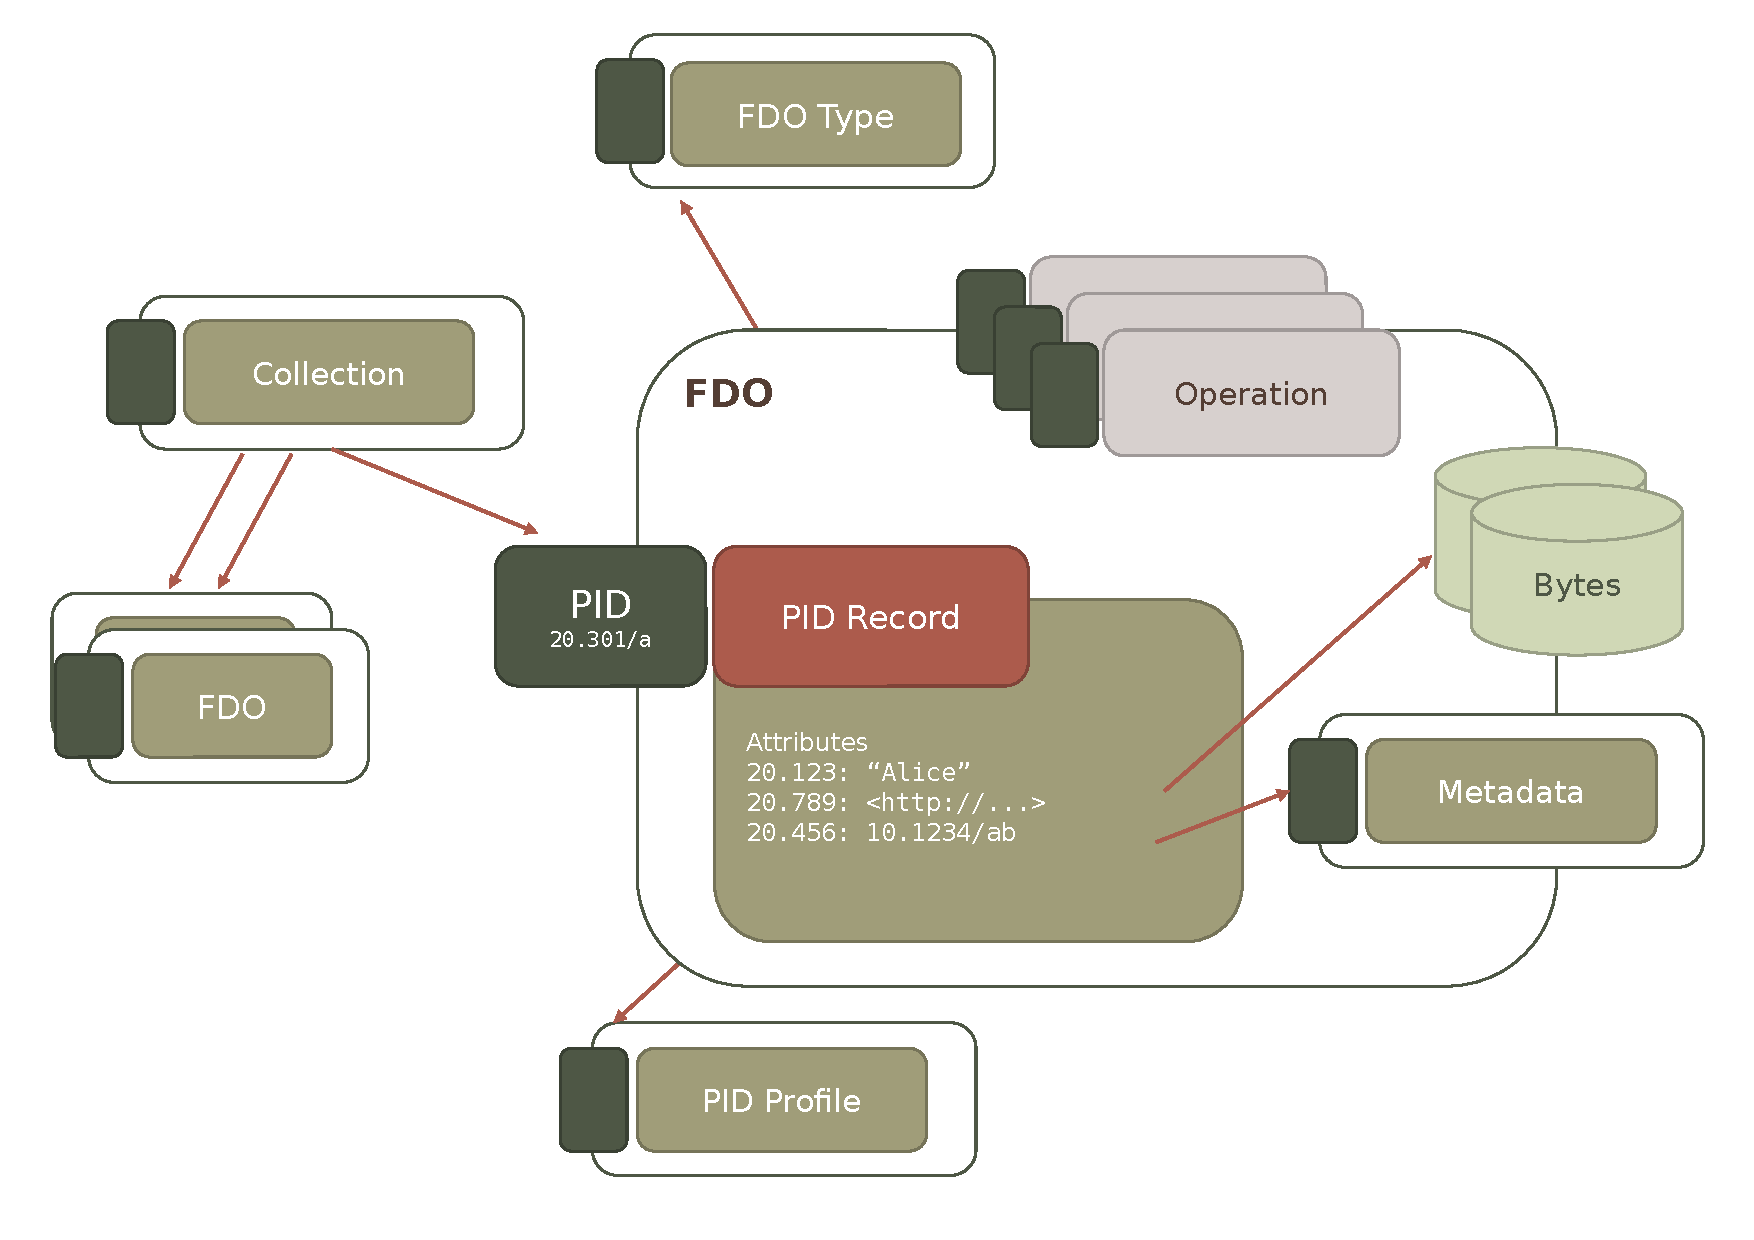
\includegraphics[width=\textwidth]{figures/ch03/fdo.pdf}
    \caption[Idealised overview of a FAIR Digital Object]{\textbf{Idealised overview of a FAIR Digital Object}. The persistent identifier (PID), (e.g. a Handle, DOI or permalink), refers to an FDO through a PID Record, which may reference downloadble bytes, and optionally additional metadata in another FDO. A series of operations are accessible from an FDO (for instance retrieving the bytes). Similar to in object-oriented programming, the FDO Type indicates which operations and attributes are applicable to an FDO. FDOs can be cross-related using the PIDs, a Collection is then another such FDO which aggregates other FDOs by reference. The configuration shown here is just one of many possible \cite{fdo-ConfigurationTypes}, along with the choice of PID system, nature of the PID Record and metadata vocabularies, which are identified through an FDO Profile. In practice, some compromises from this idealised picture are taken depending on the implementation, for instance attribute keys may be simple strings rather than PIDs, and default operations are not explicitly declared.
    }
  \label{ch3:fig:fdo}
\end{figure}

Recently, FDOs have been recognised by the European Open Science Cloud (\footurl{https://eosc.eu/}{EOSC}) as a suggested part of its Interoperability Framework \cite{eosc-interop-framework}, in particular for deploying active and interoperable FAIR resources that are \emph{machine actionable}. Development of the FDO concept continued within Research Data Alliance (\footurl{https://www.rd-alliance.org/}{RDA}) groups and EOSC projects like \footurl{https://www.go-fair.org/}{GO-FAIR}, concluding with a set of guidelines for implementing FDO \cite{bonino2019}. The \footurl{https://fairdo.org/}{FAIR Digital Objects Forum} has since taken over the maturing of FDO through focused working groups which have currently drafted several more detailed specification documents (see \emph{Next steps for FDO} \vpageref{ch3:next-step-fdo}).

\subsection{FDO approaches}\label{ch3:fdo-approaches}

FDO is an evolving concept. A set of FDO Demonstrators \cite{wittenburgFAIRDigitalObject2022b} highlights how current adapters are approaching implementations of FDO from different angles:

\begin{itemize}
\tightlist
\item
  Building on the Digital Object concept, using the simplified DOIP v2.0 \cite{DONA 2018} specification, which detail how to exchange JSON objects through a text-based protocol\footnote{For a brief introduction to DOIP 2.0, see \cite{DOIPExamplesCordraa}} (usually TCP/IP over TLS). The main DOIP operations are retrieving, creating and updating digital objects. These are mostly realised using the reference implementation Cordra \cite{tupelo-schneckrobertBriefIntroductionCordra2022}. FDO types are registered in the local Cordra instance, where they are specified using JSON Schema \cite{Draftbhuttonjsonschema} and PIDs are assigned using the Handle system. Several type registries have been established.
\item
  Following the Linked Data approach, but using the DOIP protocol, e.g.~using JSON-LD and schema.org within DOIP in Materal Sciences archives \cite{10.1002/jcc.26842}.
\item
  Approaching the FDO principles from existing Linked Data practices on the Web, e.g.~WorkflowHub use of RO-Crate and schema.org \cite{10.3897/rio.8.e93937}.
\end{itemize}

From this it becomes apparent that there is a potentially large overlap between the goals and approaches of FAIR Digital Objects and Linked Data, which we will cover \vpageref{ch3:ld}.


\subsection{Next steps for FDO}\label{ch3:next-step-fdo}

The FAIR Digital Object Forum \cite{FAIRDigitalObjects} working groups have prepared detailed requirement documents \cite{fdo-Specs} setting out the path for realising FDOs, named \emph{FDO Recommendations}. As of 2023-06-17, most of these documents are open for public review, while some are still in draft stages for internal review. As these documents clarify the future aims and focus of FAIR Digital Objects \cite{fdo-Roadmap}, we provide a brief summary of each:

\textbf{FAIR Digital Object Overview and Specifications} \cite{fdo-Overview} is a comprehensive overview of FAIR Digital Object specifications listed below. It serves as a primer that introduces FDO concepts and the remaining documents. It is accompanied by an FDO Glossary \cite{fdo-Glossary}.

The \textbf{FDO Forum Document Standards} \cite{fdo-DocProcessStd} documents the recommendation process within the forum, starting at \emph{Working Draft} (WD) status within the closed working group and later within the open forum, then \emph{Proposed Recommendation} (PR) published for public review, finalised as \emph{FDO Forum Recommendation} (REC) following any revisions. In addition, the forum may choose to \emph{endorse} existing third-party notes and specifications.

The \textbf{FDO Requirement Specifications} \cite{fdo-RequirementSpec} is an update of \cite{bonino2019} as the foundational definition of FDO. This sets the criteria for classifying an digital entity as a FAIR Digital Object, allowing for multiple implementations. The requirements shown in Table \vref{ch3:fdo-checks} are largely equivalent, but in this specification clarified with references to other FDO documents.

The \textbf{Machine actionability} \cite{fdo-MachineActionDef} sets out to define what is meant by \emph{machine actionability} for FDOs. \emph{Machine readable} is defined as elements of bit-sequences defined by structural specification, \emph{machine interpretable} elements that can be identified and related with semantic artefacts, while \emph{machine actionable} are elements with a type with operations in a symbolic grammar. The document largely describes requirements for resolving an FDO to metadata, and how types should be related to possible operations.

\textbf{Configuration Types} \cite{fdo-ConfigurationTypes} classifies different granularities for organising FDOs in terms of PIDs, PID Records, Metadata and bit sequences, e.g.~as a single FDO or several daisy-chained FDOs. Different patterns used by current DOIP deployments are considered, as well as FAIR Signposting \cite{vandesompel2015,Van de Sompel 2022}.

\textbf{PID Profiles \& Attributes} \cite{fdo-PIDProfileAttributes} specifies that PIDs must be formally associated with a \emph{PID Profile}, a separate FDO that defines attributes required and recommended by FDOs following said profile. This forms the \emph{kernel attributes}, building on recommendations from RDA's \emph{PID Information Types} working group \cite{weigelRDARecommendationPID2018}. This document makes a clear distinction between a minimal set of attributes needed for PID resolution and FDO navigation, which needs to be part of the \emph{PID Record} \cite{islam_2023}, compared with a richer set of more specific attributes as part of the \emph{metadata} for an FDO, possibly represented as a separate FDO.

\textbf{Kernel Attributes \& Metadata} \cite{fdo-KernelAttributes} elaborates on categories of FDO Mandatory, FDO Optional and Community Attributes, recommending kernel attributes like \texttt{dateCreated}, \texttt{ScientificDomain}, \texttt{PersistencePolicy}, \texttt{digitalObjectMutability}, etc. This document expands on RDA Recommendation on PID Kernel Information \cite{weigelRDARecommendationPID2018}. It is worth noting that both documents are relatively abstract and do not establish PIDs or namespaces for the kernel attributes.

\textbf{Granularity, Versioning, Mutability} \cite{fdo-Granularity} considers how granularity decisions for forming FDOs must be agreed by different communities depending on their pragmatic usage requirements. The affect on versioning, mutability and changes to PIDs are considered, based on use cases and existing PID practices.

\textbf{DOIP Endorsement Request} \cite{fdo-DOIPEndorsement} is an endorsement of the DOIP v2.0 \cite{DONA 2018} specification as a potential FDO implementation, as it has been applied by several institutions \cite{wittenburgFAIRDigitalObject2022b}. The document proposes that DOIP shall be assessed for completeness against FDO -- in this initial draft this is justified as \emph{``we can state that DOIP is compliant with the FDO specification documents in process''} (the documents listed above).

\textbf{Upload of FDO} \cite{fdo-FDO-Upload} illustrates the operations for uploading an FDO to a repository, what checks it should do (for instance conformance with the PID Profile, if PIDs resolve). ResourceSync \cite{ResourceSyncFrameworkSpecification} is suggested as one type of service to list FDOs. This document highlights potential practices by repositories and their clients, without adding any particular requirements.

\textbf{Typing FAIR Digital Objects} \cite{fdo-TypingFDOs} defines what \emph{type} means for FDOs, primarily to enable machine actionability and to define an FDO's purpose. This document lays out requirements for how \emph{FDO Types} should themselves be specified as FDOs, and how an \emph{FDO Type Framework} allows organising and locating types. Operations applicable to an FDO is not predefined for a type, however operations naturally will require certain FDO types to work. How to define such FDO operations is not specified.

\textbf{Implementation of Attributes, Types, Profiles and Registries} \cite{fdo-ImplAttributesTypesProfiles} details how to establish FDO registries for types and FDO profiles, with their association with PID systems. This document suggest policies and governance structures, together with guidelines for implementations, but without mandating any explicit technology choices. Differences in use of attributes are examplified using FDO PIDs for scientific instruments, and the proto-FDO approach of \footurl{https://de.dariah.eu/}{DARIAH-DE} \cite{schwardmannTwoExamplesHow2022}.

%See bibliography \vref*{ch3:fdo-bibliography} for the citation per document above.
It is worth pointing out that, except for the DOIP endorsement, all of these documents are conceptual, in the sense that they permit any technical implementation of FDO, if used according to the recommendations. 
Existing FDO implementations \cite{wittenburgFAIRDigitalObject2022b} are thus not fully consolidated in choices such as protocols, type systems and serialisations -- this divergence and corresponding additional technical requirements mean that FDOs are not yet in a single ecosystem.


\section{From the Semantic Web to Linked Data}\label{ch3:ld}

In order to describe \emph{Linked Data} as it is used today, we'll start with an (opinionated) description of the evolution of its foundation, the \emph{Semantic Web}.

\subsection{A brief history of the Semantic Web}\label{ch3:semweb}

The \textbf{Semantic Web} was developed as a vision by Tim Berners-Lee \cite{berners-leeWeavingWebOriginal1999}, at a time that the Web had already become widely established for information exchange, being a global set of hypermedia documents which are cross-related using universal links in the form of URLs. The foundations of the Web (e.g.~URLs, HTTP, SSL/TLS, HTML, CSS, ECMAScript/JavaScript, media types) were standardised by \footurl{https://www.w3.org/standards/}{W3C}, \footurl{https://www.ecma-international.org/}{Ecma}, \footurl{https://www.ietf.org/standards/}{IETF} and later \footurl{https://whatwg.org/}{WHATWG}. The goal of Semantic Web was to further develop the machine-readable aspects of the Web, in particular adding \emph{meaning} (or semantics) to not just the link relations, but also to the \emph{resources} that the URLs identified, and for machines thus being able to meaningfully navigate across such resources, e.g.~to answer a particular query.

Through W3C, the Semantic Web was realised with the Resource Description Framework (RDF) \cite{w3-rdf11-primer} that used \emph{triples} of subject-predicate-object statements, with its initial serialisation format \cite{w3-rdf-syntax99} being RDF/XML (XML was at the time seen as a natural data-focused evolution from the document-centric SGML and HTML).

While triple-based knowledge representations were not new \cite{stanczykProcessModellingInformation1987}, the main innovation of RDF was the use of global identifiers in the form of URIs\footnote{URIs \cite{rfc3986} are generalised forms of URLs that include locator-less identifiers such as ISBN book numbers (URNs). The distinction between locator-full and locator-less identifiers have weakened in recent years \cite{InfoURIRegistry}, for instance DOI identifiers now are commonly expressed with the prefix \texttt{https://doi.org/} rather than as URNs with \texttt{info:doi:} given that the URL/URN gap has been bridged by HTTP resolvers and the use of Persistent Identifiers (PIDs) \cite{jutyIdentifiersOrgMIRIAM2011}. RDF 1.1 formats use Unicode to support \emph{IRIs} \cite{Duerst 2005}, which extends URIs to include international characters and domain names.} as the primary identifier of the \emph{subject} (what the statement is about), \emph{predicate} (relation/attribute of the subject) and \emph{object} (what is pointed to) -- see listing \vref{ch3:triples}. By using URIs not just for documents\footnote{URIs can also identify \emph{non-information resources} for any kind of physical object (e.g.~people), such identifiers can resolve with \texttt{303\ See\ Other} redirections to a corresponding \emph{information resources} \cite{sauermannCoolURIsSemantic2011}.}, the Semantic Web builds a self-described system of types and properties, where the meaning of a relation can be resolved by following its hyperlink to the definition within a \emph{vocabulary}. By applying these principles as well to any kind of resource that could be described at a URL, this then forms a global distributed Semantic Web (figure \vref{ch3:fig:jsonld}).


\begin{figure}[hbt!]
  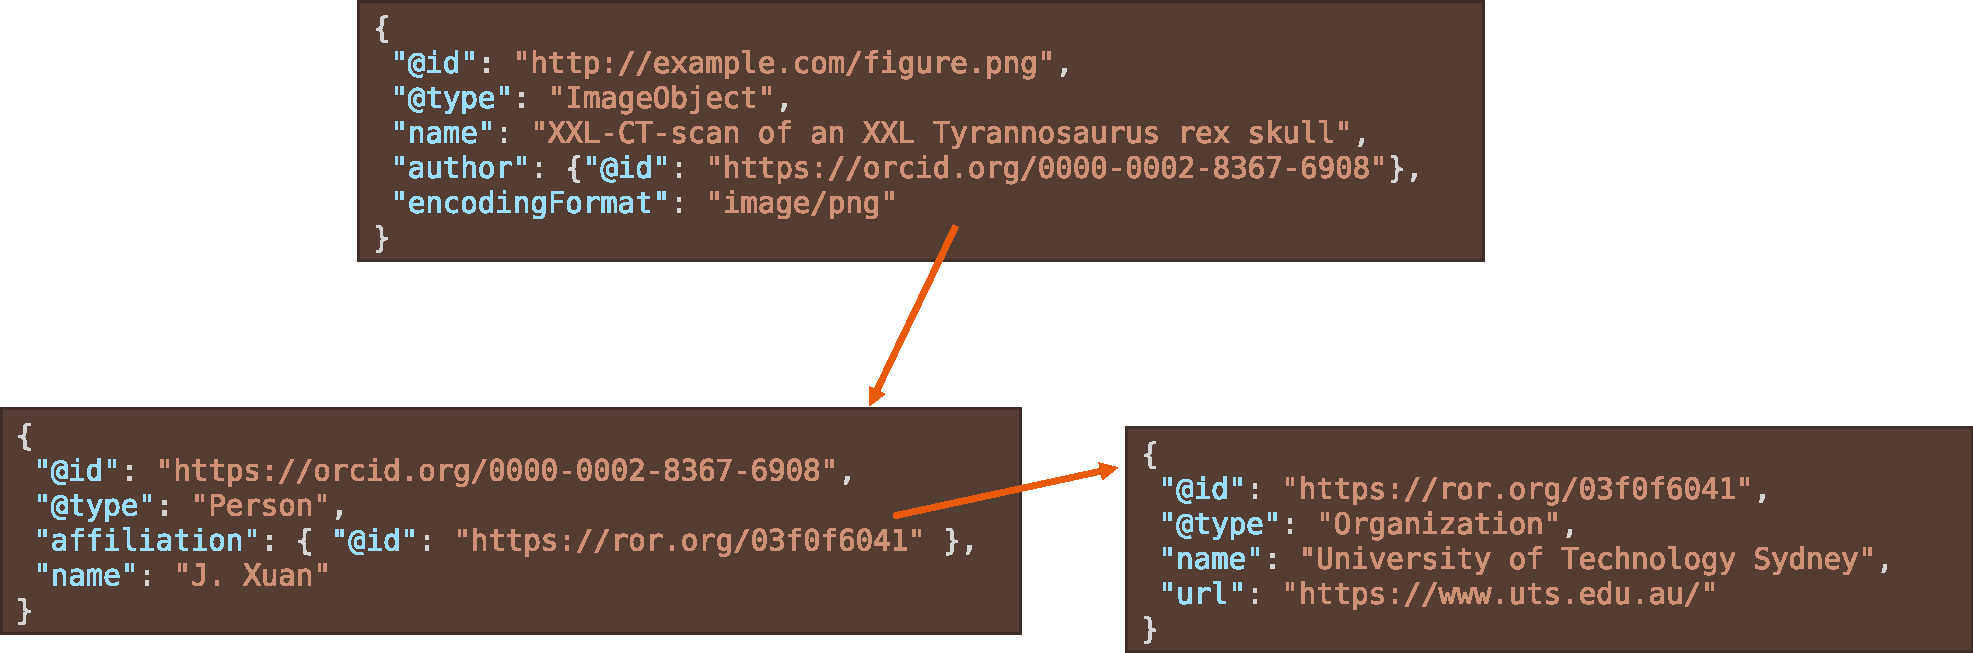
\includegraphics[width=\textwidth]{figures/ch03/jsonld.pdf}
    \caption[Example of linked RDF resources]{\textbf{Example of linked RDF resources}. Each \emph{resource} in an RDF graph has an identifier, here shown as absolute URIs, a type and a series of properties. A property value can either be a \emph{literal} (e.g. "Josiah Carberry") or another resource (e.g. \url{https://ror.org/03f0f6041}). A graph is formed by such cross-references across resources.
    In the idealised Semantic Web, every URI would resolve to a description of its resource in RDF. In practice there can be misalignments of identifiers, vocabularies, resolution mechanisms, or simply lack of RDF adoptation. Therefore any RDF graph can describe any Web resource identified by its URI, and these descriptipns, using an \emph{open world assumption} \cite{openworld?}, can be merged with other graphs describing the same resource.
    For brevity and comparison from later chapters this figure uses the newer RDF format JSON-LD \cite{w3-json-ld}, 
    which can be expanded with context \url{http://schema.org/} (not shown) to anchor types and 
    properties as absolute URIs and generate corresponding RDF triples (listing \vref{ch3:triples}). 
    }
  \label{ch3:fig:jsonld}
\end{figure}

\begin{listing}
  \footnotesize
  \begin{verbatim}
    <http://example.com/figure.png> a <http://schema.org/ImageObject> .
    <http://example.com/figure.png> <http://schema.org/name> "XXL-CT-scan of an XXL Tyrannosaurus rex skull" .
    <http://example.com/figure.png> <http://schema.org/author> <https://orcid.org/0000-0002-1825-0097> .
    <http://example.com/figure.png> <http://schema.org/encodingFormat> "image/png" .

    <https://orcid.org/0000-0002-1825-0097> a <http://schema.org/Person> .
    <https://orcid.org/0000-0002-1825-0097> <http://schema.org/name> "Josiah Carberry" .
    <https://orcid.org/0000-0002-1825-0097> <http://schema.org/affiliation> <https://ror.org/03f0f6041> .

    <https://ror.org/03f0f6041> a <http://schema.org/Organization> .
    <https://ror.org/03f0f6041> <http://schema.org/name> "University of Technology Sydney" .
    <https://ror.org/03f0f6041> <http://schema.org/url> "https://www.uts.edu.au/" .
  \end{verbatim}  
  \caption[Example of RDF triples]{\textbf{Example of RDF triples} corresponding to figure \vref{ch3:fig:jsonld} after expansion with a JSON-LD context. In this example the properties and types are all using the same vocabulary \cite{schema.org}, in the traditional Semantic Web it is common to mix vocabularies. This listing uses the RDF syntax N-Triples \cite{n-triples} where each line indicates \emph{subject}, \emph{predicate} and \emph{object}. Notable here is the syntactical difference between an URI reference that is part of the graph \texttt{<https://ror.org/03f0f6041>} and a string literal \texttt{"https://www.uts.edu.au/"} which just happens to be a URI. }
  \label{ch3:triples}
\end{listing}

The early days of the Semantic Web saw fairly lightweight approaches with the establishment of vocabularies such as FOAF (to describe people and their affiliations) and Dublin Core (for bigbliographic data). Vocabularies themselves were formalised using RDFS or simply as human-readable HTML web pages defining each term. The main approach of this \emph{Web of Data} was that a URI identified a \emph{resource} (e.g.~an author) with a HTML \emph{representation} for human readers, along with a RDF representation for machine-readable data of the same resource. By using \emph{content negotiation} in HTTP\footnote{\url{https://developer.mozilla.org/en-US/docs/Web/HTTP/Content_negotiation}}, the same identifier could be used in both views, avoiding \texttt{index.html} vs \texttt{index.rdf} exposure in the URLs. The concept of \emph{namespaces} gave a way to give a group of RDF resources with the same URI base from a Semantic Web-aware service a common \emph{prefix}, avoiding repeated long URLs.

The mid-2000s saw large academic interest and growth of the Semantic Web, with the development of more formal representation system for ontologies, such as OWL \cite{w3-owl2-overview}, allowing complex class hierarchies and logic inference rules following \emph{open world} paradigm. (e.g.~a \emph{ex:Parent} is equivalent to a subclass of \emph{foaf:Person} which must \emph{ex:hasChild} at least one \emph{foaf:Person}, then if we know \emph{:Alice a ex:Parent} we can infer \emph{:Alice ex:hasChild {[}a foaf:Person{]}} even if we don't know who that child is). More human-readable syntaxes for RDF such as Turtle evolved at this time, and conferences such as \footurl{https://iswc2022.semanticweb.org/}{ISWC} \cite{horrocksSemanticWebISWC2002} gained traction, with a large interest in knowledge representation and logic systems based on Semantic Web technologies evolving at the same time.

Established Semantic Web services and standards include: SPARQL \cite{w3-sparql11-overview} (pattern-based triple queries), \footurl{https://www.w3.org/TR/rdf11-concepts/\#section-dataset}{named graphs} \cite{w3-rdf11-concepts} (triples expanded to \emph{quads} to indicate statement source or represent conflicting views), triple/quad stores (graph databases such as OpenLink Virtuoso, GraphDB, 4Store), mature RDF libraries (including Redland RDF, Apache Jena, Eclipse RDF4J, RDFLib, RDF.rb, rdflib.js), and graph visualisation.

RDF is one way to implement \emph{knowledge graphs}, a system of named edges and nodes\footnote{In RDF, each triple represent an edge that is named using its property URI, and the nodes are subject/object as URIs, blank nodes or (for objects) typed literal values \cite{w3-rdf11-primer}.} \cite{nurdiati2008}, which when used to represent a sufficiently detailed model of the world, can then be queried and processed to answer detailed research questions.
The creation of RDF-based knowledge graphs grew particularly in fields like bioinformatics, e.g.~for describing genomes and proteins \cite{gobleStateNationData2008c,williamsOpenPHACTSSemantic2012c}. In theory, the use of RDF by the life sciences would enable interoperability between the many data repositories and support combined views of the many aspects of bio-entities -- however in practice most institutions ended up making their own ontologies and identifiers, for what to the untrained eye would mean roughly the same. One can argue that the toll of adding the semantic logic system of rich ontologies meant that small, but fundamental, differences in opinion (e.g.~\emph{should a gene identifier signify just the particular DNA sequence letters, or those letters as they appear in a particular position on a human chromosome?}) led to large differences in representational granularity, and thus needed different identifiers.

Facing these challenges, thanks to the use of universal identifiers in the form of URIs, \emph{mappings} could retrospectively be developed not just between resources, but also across vocabularies. Such mappings can be expressed themselves using lightweight and flexible RDF vocabularies such as SKOS \cite{w3-skos-primer} (e.g.~\texttt{dct:title\ skos:closeMatch\ schema:name} to indicate near equivalence of two properties). Exemplifying the need for such cross-references, automated ontology mappings have identified large potential overlaps, like 372 definitions of \texttt{Person}) \cite{huHowMatchableAre2011a}.

The move towards \emph{Open Science} data sharing practices did from the late 2000s encourage knowledge providers to distribute collections of RDF descriptions as downloadable \emph{datasets} \footnote{\emph{Datasets} that distribute RDF graphs should not be confused with \emph{RDF Datasets} used for partitioning \emph{named graphs}, see \url{https://www.w3.org/TR/rdf11-concepts/\#section-dataset}}, so that their clients can avoid thousands of HTTP requests for individual resources. This enabled local processing, mapping and data integration across datasets (e.g.~Open PHACTS \cite{grothAPIcentricLinkedData2014b}), rather than relying on the providers' RDF and SPARQL endpoints (which could become overloaded when handling many concurrent, complex queries).

With these trends, an emerging problem was that adopters of the Semantic Web primarily utillised it as a set of graph technologies, with little consideration to existing Web resources. This meant that links stayed mainly within a single information system, with little URI reuse even with large term overlaps \cite{kamdarSystematicAnalysisTerm2017a}. Just like \emph{link rot} affect regular Web pages and their citations from scholarly communication \cite{kleinScholarlyContextNot2014a}, for a majority of described RDF resources in the \footurl{https://lod-cloud.net/}{Linked Open Data} (LOD) Cloud's gathering of more than thousand datasets, unfortunately do not actually link to (still) downloadable (\emph{dereferenceable}) Linked Data \cite{polleresMoreDecentralizedVision2020a}. Another challenge facing potential adopters is the plethora of choices, not just to navigate, understand and select to reuse the many possible vocabularies and ontologies \cite{carrieroLandscapeOntologyReuse2020a}, but also technological choices on RDF serialisation (at least \footurl{https://www.w3.org/TR/rdf11-primer/\#section-graph-syntax}{7 formats}), type system (RDFS \cite{w3-rdf-schema}, OWL \cite{w3-owl2-overview}, OBO \cite{tirmiziMappingOBOOWL2011a}, SKOS \cite{w3-skos-primer}), and deployment challenges \cite{sauermannCoolURIsSemantic2011} (e.g. hash vs slash in namespaces, HTTP status codes and PID redirection strategies).

\subsection{Linked Data: Rebuilding the Web of Data}\label{ch3:ld-web}

The \textbf{Linked Data} (LD) concept \cite{Bizer 2009} was kickstarted as a set of best practices \cite{LinkedDataDesign} to bring the Web aspect of the Semantic Web back into focus. Crucial to Linked Data is the \emph{reuse of existing URIs}, rather than making new identifiers. This means a loosening of the semantic restrictions previously applied, and an emphasis on building navigable data resources, rather than elaborate graph representations.

Vocabularies like \footurl{https://schema.org/}{schema.org} evolved not long after, intended for lightweight semantic markup of existing Web pages, primarily to improve search engines' understanding of types and embedded data. In addition to several such embedded \emph{microformats} \cite{OpenGraphProtocol,w3-rdfa-primer,HTMLStandard}, we find JSON-LD \cite{w3-json-ld} as a Web-focused RDF serialisation that aims for improved programmatic generation and consumption, including from Web applications. JSON-LD is as of 2023-05-18 used\footnote{Presumably this large uptake of JSON-LD is mainly for the purpose of Search Engine Optimisation (SEO), with typically small amounts of metadata which may not constitute Linked Data as introduced above, however this deployment nevertheless constitute machine-actionable structured data.} by 45\% of the top 10 million websites \cite{UsageStatisticsJSONLD}.

Recently there has been a renewed emphasis to improve the \emph{Developer Experience} \cite{DesigningLinkedData2018} for consumption of Linked Data, for instance RDF Shapes -- expressed in SHACL \cite{w3-shacl} or ShEx \cite{ShapeExpressionsShEx} -- can be used to validate RDF Data \cite{gayoValidatingRDFData2017a,thorntonUsingShapeExpressions2019a} before consuming it programmatically, or reshaping data to fit other models. While a varied set of tools for Linked Data consumptions have been identified, most of them still require developers to gain significant knowledge of the underlying Semantic Web technologies, which hampers adaption by non-LD experts \cite{klimekSurveyToolsLinked2019a}, which then tend to prefer non-semantic two-dimensional formats such as CSV files.

A valid concern is that the Semantic Web research community has still not fully embraced the Web, and that the ``final 20\%'' engineering effort is frequently overlooked in favour of chasing new trends such as Big Data and AI, rather than making powerful Linked Data technologies available to the wider groups of Web developers \cite{verborghSemanticWebIdentity2020a}. One bridging gap here by the Linked Data movement has been ``Linked Data by stealth'' approaches such as structured data entry spreadsheets powered by ontologies \cite{wolstencroftRightFieldEmbeddingOntology2011b}, the use of Linked Data as part of REST Web APIs \cite{pageRESTLinkedData2011}, and as shown by the big uptake by publishers to annotate the Web using schema.org \cite{bernsteinNewLookSemantic2016a}, with vocabulary use patterns documented by copy-pastable JSON-LD examples, rather than by formalised ontologies or developer requirements to understand the full Semantic Web stack.

Linked Data provides technologies that have evolved over time to satisfy its primary purpose of data interoperability. The needs to embrace the Web and developer experience have been central lessons learned.  In contrast, FDO is a new approach with many different potential paths forward, and having a partial overlap with the aims of Linked Data


\chapter{Comparing FDO and Linked Data as FAIR implemantations}
\label{chapter:fdo}

To investigate \textbf{RQ1} (\vpageref*{rq1}) this chapter evaluates both Linked Data and FAIR Digital Object (FDO) as ways to realize the FAIR principles. Section \ref{ch3:evaluating-fdo-ld} compares the two approaches as global distributed object systems, and discusses what lessons can be learnt across the communities, taking into consideration the history covered by section \ref{chapter:background}.

Section \ref{ch2:updating-linked-data-practices-for-fair-digital-object-principles} proposes how the FDO principles can be achieved using Linked Data standards, which is explored further in the following chapters.

\section{Evaluating FAIR Digital Object and Linked Data as distributed object systems}\label{ch3:evaluating-fdo-ld}

FAIR Digital Object (FDO) is an emerging concept that is highlighted by European Open Science Cloud (EOSC) as a potential candidate for building an ecosystem of machine-actionable research outputs. In this work we systematically evaluate FDO and its implementations as a global distributed object system, by using five different conceptual frameworks that cover interoperability, middleware, FAIR principles, EOSC requirements and FDO guidelines themself.

We compare the FDO approach with established Linked Data practices and the existing Web architecture, and provide a brief history of the Semantic Web\footnote{
  See section \vref{ch3:background} for background information on Linked Data and FDO}. while discussing why these technologies may have been difficult to adopt for FDO purposes. We conclude with recommendations for both Linked Data and FDO communities to further their adaptation and alignment.

\subsection{Introduction}\label{ch3:introduction}

The FAIR principles \cite{Wilkinson 2016} encourage sharing of scientific data with machine-readable metadata and the use of interoperable formats, and are being adapted by a wide range of research infrastructures. They have been recognised by the research community and policy makers as a goal to strive for \cite{h2020fair2016}. In particular, the European Open Science Cloud \footurl{https://www.eosc.eu/}{(EOSC)} has promoted adaptation of FAIR data sharing of data resources across electronic research infrastructures \cite{Mons 2017}. The EOSC Interoperability Framework \cite{eosc-interop-framework} puts particular emphasis on how interoperability can be achieved technically, semantically, organisationally, and legally -- laying out a vision of how data, publication, software and services can work together to form an ecosystem of digital objects that are extensively described. Such descriptions for interoperability connect a range of information -- from protocols and presentations, to hardware designs and scientific workflows, including extensive metadata of the information itself.

Specifically, the EOSC Interoperability framework highlights the emerging FAIR Digital Object (FDO) concept \cite{schultesFAIRPrinciplesDigital2019a} as a possible foundation for building a semantically interoperable ecosystem to fully realise the FAIR principles beyond individual repositories and infrastructures. The FDO approach has great potential, as it proposes strong requirements for identifiers, types, access and formalises interactive operations on objects.

In other discourse, Linked Data \cite{Bizer 2009} has been seen as an established set of principles based on Semantic Web technologies that can achieve the vision of the FAIR principles \cite{boninodasilvasantosFAIRDataPoints2016a,Hasnain 2018}. Yet regular researchers and developers of emerging platforms for computation and data management are reluctant to adapt such a ``FAIR Linked Data'' approach fully \cite{verborghSemanticWebIdentity2020a}, opting instead for custom in-house models and JSON-derived formats from RESTful Web services \cite{merono-penuelaConclusionFutureChallenges2021a,neumannAnalysisPublicREST2021a}. While such focus on simplicity allows rapid development and highly specialised services, it raises wider concerns about interoperability \cite{turcoaneLinkedDataJSONLD2014a,wilkinsonWorkflowsWhenParts2022b}.

One challenge that may, perhaps counter-intuitively, steer developers towards a not-invented-here mentality \cite{stefiDevelopersMakeUnbiased2015,stefiDevelopReuseTwo2015a} when exposing their data on the Web is the heterogeneity and apparent complexity of Semantic Web approaches themselves \cite{merono-penuelaWebDataApis2021b}.

These approaches -- FDO and Linked Data -- thus, form two of the major avenues for allowing developers and the wider research community to achieve the goal of FAIR data. Given their importance, in this article, we compare FAIR Digital Objects with Linked Data and the Web architecture in the context of the discourse around FAIR data.

Concretely, the contribution of this paper is a {\bf systematic comparison between FDO and Linked Data using 5 different conceptual frameworks} that capture different perspectives on interoperability and readiness for implementation.

In chapter \vref{ch3:background} we gave a background primer on FDO and Linked Data to provide a foundation for this work. The rest of this section is organised as follows:  In the Method section \vpageref{ch3:method}, we introduce the conceptual frameworks we use for comparison. Sub sequently, in the Results section \vpageref{ch3:results}, we systematically step through the outcomes of applying these frameworks to both FDO and Linked Data. For each framework, we derive key observations. We end \vpageref{ch3:discussion} with a discussion of these results and their implications for both approaches and conclude.


\subsection{Method}\label{ch3:method}

\subsubsection{Comparing FDO and existing approaches}\label{ch3:comparing}

Our main motivation for this article is to investigate how FAIR Digital Objects may differ from the learnt experiences of Linked Data and the Web. We also aim to reflect back from FDO's motivation of machine-actionability to consider the Web as a distributed computational system.

To better understand the relationship between the FDO framework and other existing approaches, we use the following for analysis:

\begin{enumerate}
\tightlist
\item
  An Interoperability Framework and Distributed Platform for Fast Data Applications \cite{delgadoInteroperabilityFrameworkDistributed2016a}, which proposes quality measurements for comparing how frameworks support interoperability, particularly from a service architectural view.
\item
  The FAIR Digital Object guidelines \cite{bonino2019}, validated against its current implementations for completeness.
\item
  A Comparison Framework for Middleware Infrastructures \cite{zarrasComparisonFrameworkMiddleware2004a}, which suggest dimensions like openness, performance and transparency, mainly focused on remote computational methods.
\item
  Cross-checks against RDA's FAIR Data Maturity Model \cite{bahimFAIRDataMaturity2020a} to find how the FAIR principles are achieved in FDO, in particular considering access, sharing and openness.
\item
  EOSC Interoperability Framework \cite{eosc-interop-framework} which gives recommendations for technical, semantic, organisational and legal interoperability, particularly from a metadata perspective.
\end{enumerate}

Conceptual framework 1, 3, 5 consider more general views of interoperability between systems, whereas frameworks 2 and 4 are developed specifically for addressing FAIR principles. 

The reason for this wide-ranged comparison is to exercise the different dimensions that together form FAIR Digital Objects: Data, Metadata, Service, Access, Operations, Computation.
We have left out further comparisons on type systems, persistent identifiers and social aspects as principles and practices within these dimensions are still taking form within the FDO community (as detailed in section \vpageref{ch3:next-step-fdo}).

Some of these frameworks invite a comparison on a conceptual level, while others relate better to implementations and current practices. For these conceptual comparisons we consider FAIR Digital Objects and the Web broadly. For implementations we contrast the main FDO realisation using the DOIPv2 protocol \cite{DONA 2018} against Linked Data as implemented in general practice\footnote{For further background on FDO implemented with Linked Data see \cite{bonino2021,10.3897/rio.8.e94501}}.

For all our comparisons, our process was to perform a mapping between the relevant specifications and/or implementation and the given conceptual model through detailed reading of the defining documents. We aim in all cases for traceability between the given specification and our mapping such that readers can validate our analysis.

\subsection{Results}\label{ch3:results}

\subsubsection{Considering FDO/Web as interoperability framework for Fast Data}\label{ch3:interoperability-compare}


The Interoperability Framework for Fast Data Applications \cite{delgadoInteroperabilityFrameworkDistributed2016a} categorises interoperability between applications along 6 strands, covering different architectural levels: from \emph{symbiotic} (agreement to cooperate) and \emph{pragmatic} (ability to choreograph processes), through \emph{semantic} (common understanding) and \emph{syntactic} (common message formats), to low-level \emph{connective} (transport-level) and \emph{environmental} (deployment practices).

We have chosen to investigate using this framework as it covers the higher levels of the OSI Model \cite{stallingsHandbookComputercommunicationsStandards1990} better with regards to automated machine-to-machine interaction (and thus interoperability), which is a crucial aspect of the FAIR principles. In Table \ref{ch3:fdo-web-interoperability-framework} we use the interoperability framework to compare the current FAIR Digital Object approach against the Web and its Linked Data practices.

\renewcommand*{\arraystretch}{1.4}
\begin{longtable}[]{@{}
  >{\raggedright\arraybackslash}p{(\columnwidth - 4\tabcolsep) * \real{0.1642}}
  >{\arraybackslash}p{(\columnwidth - 4\tabcolsep) * \real{0.4179}}
  >{\arraybackslash}p{(\columnwidth - 4\tabcolsep) * \real{0.4179}}@{}}
\caption[Considering FDO and Web according to Interoperability Framework for Fast Data]{Considering FDO and Web according to the quality levels of the Interoperability Framework for Fast Data \cite{delgadoInteroperabilityFrameworkDistributed2016a}.
\label{ch3:fdo-web-interoperability-framework}}\tabularnewline
\toprule
Quality & 
FDO w/ DOIP & 
Web w/ Linked Data \\
\midrule
\endfirsthead
\toprule
Quality &
FDO w/ DOIP & 
Web w/ Linked Data \\
\midrule
\endhead
\textbf{Symbiotic}: \emph{to what extent multiple applications can agree to interact, align, collaborate or cooperate}
  & The purpose of FDO is to enable federated machine actionable digital objects for scholarly purposes, in practice this also requires agreement of compatibility between FDO types. FDO encourages research communities to develop common type registries to be shared across instances. In current DOIP practice, each service have their own types, attributes and operations. The wider symbiosis is consistent use of PIDs.
  & The Web is loosely coupled and encourages collaboration and linking by URL. In practice, REST APIs \cite{fieldingArchitecturalStylesDesign2000a} end up being mandated centrally by dominant (often commercial) providers \cite{fieldingReflectionsRESTArchitectural2017a}, and the clients are required to use each API as-is with special code per service. Use of Linked Data enables common tooling and semantic mapping across differences. \\
\textbf{Pragmatic}: \emph{using interaction contracts so processes can be choreographed in workflows}
  & FDO types and operations enable detailed choreography (Canonical Workflows \cite{cwfr}). \texttt{0.TYPE/DOIPOperation} has lightweight definition of operation, \texttt{0.DOIP/Request} or \texttt{0.DOIP/Response} may give FDO Type or any other kind of ``specifics'' (incl.~human readable docs). Semantics/purpose of operations not formalised (similar operations can be grouped with \texttt{0.DOIP/OperationReference}).
  & ``Follow your nose'' crawler navigation, which may lead to frequent dead ends. Operational composition, typically within a single API provider, documented by OpenAPI 3 \cite{OpenAPISpecificationV3}, schema.org Actions \cite{SchemaOrgActions}, WSDL/SOAP \cite{w3-wsdl20-primer}, but frequently just as human-readable developer documentation with examples. \\
\textbf{Semantic}: \emph{ensuring consistent understanding of messages, interoperability of rules, knowledge and ontologies}
  & FDO semantic enable navigation and typing. Every FDO has a type. Types maintained in FDO Type registries, which may add additional semantics, e.g.~the ePIC \footurl{https://hdl.handle.net/21.11104/c1a0ec5ad347427f25d6}{PID-InfoType for Model}. No single type semantic, Type FDOs can link to existing vocabularies \& ontologies. JSON-LD used within some FDO objects (e.g.~DISSCO Digital Specimen, NIST Material Science schema) \cite{wittenburgFAIRDigitalObject2022b}
  & Lightweight HTTP semantics for authenticity/navigation. Semantic Type not commonly expressed on PID/header level, may be declared within Linked Data metadata. Semantic of type implied by Linked Data formats (e.g.~OWL2, RDFS), although choice of type system may not be explicit. \\
\textbf{Syntactic}: \emph{serialising messages for digital exchange, structure representation}
  & DOIP serialise FDOs as JSON, metadata commonly use JSON, typed with JSON Schema. Multiple byte stream attachments of any media type.
  & Textual HTTP headers (including any signposting), single byte stream of any media type, e.g.~Linked Data formats (JSON-LD, Turtle, RDF/XML) or embedded in document (HTML with RDFa, JSON-LD or Microdata). XML was previously the main syntax used by APIs, JSON is now dominant. \\
\textbf{Connective}: \emph{transferring messages to another application, e.g.~wrapping in other protocols}
  & DOIP \cite{DONA 2018} is transport-independent, commonly TLS TCP/IP port 9000, DOIP over HTTP \cite{DOIPAPIHTTPa}
  & HTTP/1.1 TCP/IP port 80 \cite{rfc2616}; HTTP/1.1+TLS, TCP/IP 443 \cite{rfc2818}; HTTP/2, as HTTP/1* but binary \cite{rfc7540}; HTTP/3, like HTTP/2+TLS but UDP \cite{rfc9114} \\
\textbf{Environmental}: \emph{how applications are deployed and affected by its environment, portability}
  & Main DOIP implementation is \footurl{https://www.cordra.org/}{\emph{Cordra}}, which can be single-instance or \footurl{https://www.cordra.org/documentation/configuration/distributed-deployment.html}{distributed}. Cordra \footurl{https://www.cordra.org/documentation/configuration/storage-backends.html}{storage backends} include file system, S3, MongoDB (itself scalable). Unique DOIP protocol can be hard to add to existing Web application frameworks, although proxy services have been developed (e.g.~B2SHARE adapter).
  & HTTP services widely deployed in a myriad of ways, ranging from single instance servers, horizontally \& vertically scaled application servers, to multi-cloud Content-Delivery Networks (CDN). Current scalable cloud technologies for Web hosting may not support HTTP features previously seen as important for Semantic Web, e.g.~content negotiation and semantic HTTP status codes. \\
\bottomrule
\end{longtable}

\paragraph{Observations}

Based on the analysis shown in Table \ref{ch3:fdo-web-interoperability-framework}, we draw the following conclusions:

The Web has already showed us how one can compose workflows of hetereogeneous Web Services \cite{wolstencroftTavernaWorkflowSuite2013d}. However, this is mostly done via developer or human interaction \cite{lamprechtPerspectivesAutomatedComposition2021b}. Similiarly, FDO does not enable automatic composition because operation semantics are not well defined. There is a question as to whether the extensive documentation and broad developer usage that is available for Web APIs could potentially be utilised for FDO.

A difference between Web technologies and FDO is the stringency of the requirements for both syntax and semantics. Whereas the Web allows many different syntactic formats (e.g.~from HTML to XML, PDFs), FDO realised with DOIP requires JSON. On the semantic front, FDO mandates that every object have a well-defined type and structured form. This is clearly not the case on the Web.

In terms of connectivity and the deployment of applications, the Web has a plethora of software, services, and protocols that are widely deployed. These have shown interoperability. The Web standards bodies (e.g.~IETF and W3C) follow the OpenStand principles \cite{ModernStandardsParadigm} to embrace openness, transparency, and broad consensus. In contrast, FDO has a small number of implementations and corresponding protocols, although with a growing community, as evidenced at the first international FDO conference \cite{looFirstInternationalConference2022}. This is not to say that it is not worth developing further Handle+DOIP implementations in the future, but we note that the current FDO functionality can easily be implemented using Web technologies, even as DOIP-over-HTTP \cite{DOIPAPIHTTPa}.

It is also a question as to whether a highly constrained protocol revolving around persistent identifiers is in fact necessary. For example, DOIs are mostly resolved on the web using HTTP redirects with the common \texttt{https://doi.org/} prefix, hiding their Handle nature as an implementation detail \cite{DOIHandbookResolution}.


\subsubsection{Mapping of Metamodel concepts}\label{ch3:mapping-of-metamodel-concepts}

The Interoperability Framework for Fast Data also provides a brief \emph{metamodel} which we use in Table \vref{ch3:metamodel-concepts} to map and examplify corresponding concepts in FDO's DOIP realization and the Web using HTTP semantics \cite{rfc9110}.

From this mapping\footnote{An equivalent SKOS mapping \cite{w3-skos-primer} is provided as part of the \href{https://w3id.org/ro/doi/10.5281/zenodo.8075229}{RO-Crate for this article} \cite{soilandreyes2023}.} we can identify the conceptual similarities between DOIP and HTTP, often with common terminology. Notable are that neither DOIP or HTTP have strong support for transactions (explored further in section \vref{ch3:middleware}), as well that HTTP has poor direct support for processes, as the Web is primarily stateless by design.

\begin{table}[h!]
  \centering
  \caption[Mapping the Interoperability Framework Metamodel concepts to FDO and Web]{Mapping the Metamodel concepts from the Interoperability Framework for Fast Data \cite{delgadoInteroperabilityFrameworkDistributed2016a} to equivalent concepts for FDO and Web.
  \label{ch3:metamodel-concepts}}\tabularnewline
   \begin{tabular}{ m{5em}  m{15em} m{15em} } 
   \hline
  Metamodel concept & 
  FDO/DOIP concept & 
  Web/HTTP concept \\ 
   \hline
  Resource	  & FDO/DO	            & Resource \\
  Service	    & DOIP service	      & Server/endpoint \\
  Transaction	& (not supported)	    & Conditional requests, \texttt{409\ Conflict} \\
  Process	    & Extended operations	& (primarily stateless), \texttt{100\ Continue}, \texttt{202\ Accepted} \\
  Operation	  & DOIP Operation	    & Method, query parameters \\
  Request	    & DOIP Request	      & Request \\
  Response	  & DOIP Response	      & Response \\
  Message	    & Segment, \texttt{requestId} 
                                    & Message, Representation \\
  Channel	    & DOIP Transport protocol (e.g.~TCP/IP, TLS). JSWS signatures.
                                    & TCP/IP, TLS, UDP \\
  Protocol  	& DOIP 2.0, ++	      & HTTP/1.1, HTTP/2, HTTP/3 \\
  Link	      & PID/Handle	        & URL \\ 
   \hline
   \end{tabular}\end{table}
  

\subsubsection{Assessing FDO implementations}\label{ch3:doip-fdo-compare}

The FAIR Digital Object guidelines \cite{bonino2019} sets out recommendations for FDO implementations. Note that the proposed update to FDO specification \cite{fdo-RequirementSpec} clarifies these definitions with equivalent identifiers\footnote{Newer \cite{fdo-RequirementSpec} renames \texttt{FDOF*} to \texttt{FDOR*} but follows same ordering.} and relates them to further FDO requirements such as FDO Data Type Registries.

In Table \vref{ch3:fdo-checks} we evaluate completeness of the guidelines in two current realizations: 1) DOIPv2 \cite{DONA 2018} and 2) Linked Data Platform \cite{w3-ldp}, as proposed by \cite{bonino2021}.
We provide our analysis of each realisation with respect to the FDO Guideline and also provide suggestions for that realisation to meet the given guideline

\begin{landscape}
  \begin{small}
  \begin{longtable}[]{@{}
    >{\centering\arraybackslash}p{(\columnwidth - 8\tabcolsep) * \real{0.1}}
    >{\raggedleft\arraybackslash}p{(\columnwidth - 8\tabcolsep) * \real{0.25}}
    >{\raggedright\arraybackslash}p{(\columnwidth - 8\tabcolsep) * \real{0.2}}
    >{\raggedleft\arraybackslash}p{(\columnwidth - 8\tabcolsep) * \real{0.25}}
    >{\raggedright\arraybackslash}p{(\columnwidth - 8\tabcolsep) * \real{0.2}}@{}}
    \caption[Checking FDO guidelines against its implementations]{Checking FDO guidelines \cite{bonino2019,fdo-RequirementSpec} against its current implementations as DOIP \cite{DONA 2018} and Linked Data Platform (LDP) \cite{bonino2021}, with suggestions for required additions.
  \label{ch3:fdo-checks}}\tabularnewline
  \toprule
  \textbf{FDO Guideline} & 
  DOIP 2.0 & 
  FDO suggestions & 
  Linked Data Platform & 
  LDP suggestion \\
  \midrule
  \endfirsthead
  \toprule
  \textbf{FDO} & 
  DOIP 2.0 & 
  FDO suggestions & 
  Linked Data Platform & 
  LDP suggestion \\
  \midrule
  \endhead
G1: \emph{invest for many decades}
  & Handle system stable for 20 years, DOIP 2.0 since 2017.
  & Ensure FDO types will not be protocol-bound as DOIP might be updated/replaced
  & HTTP stable for 30 years, Semantic Web for 20 years. \texttt{http://} URIs mostly replaced by \texttt{https://}.
  & Keep flexibility of RDF serialisation formats which may change more frequently \\
G2: \emph{trustworthiness}
  & DOI/Handle trusted by all major academic publishers and data repositories. DOIP relatively unknown, in effect only one implementation.
  & Further promote DOIP and justify its benefits. Build tutorials and OSI open source implementations. Standardise DOIP-over-HTTP alternative.
  & JSON-LD used by half of all websites \cite{UsageStatisticsJSONLD}, however previous bad experiences with Semantic Web may deter adopters
  & Ensure simplicity for end developers, rather than semantic overengineering. Example-driven documentation. \\
G3: \emph{follows FAIR principles}
  & See Table \vref{ch3:fair-data-maturity-model}
  & Ensure all FAIR principles are covered, build complete examples.
  & Touched briefly, see Table \vref{ch3:fair-data-maturity-model}
  & Add explicit expression to show each FAIR principle fulfilled. \\
G4: \emph{machine actionability}
  & CRUD and extension operations dynamically listed (see Table \vref{ch3:fdo-web-middleware})
  & Specify which operations should work for a given type, to reduce need for dynamic lookup. Specify input/output expectations formally (e.g.~JSON Schema).
  & HTTP CRUD operations, Open API (see Table \vref{ch3:fdo-web-middleware})
  & Document operations so client can make subsequent HTTP calls. \\
G5: \emph{abstraction principle}
  & Handle PIDs as abstraction base. DOIP operations can use any transport protocol.
  & Document transport protocols as FDOs, recommend which transport to use.
  & URI as abstraction base. Does not specify PID requirements.
  & Give stronger deployment recommendations. \\
G6: \emph{stable binding between entities}
  & Machine-navigation through PIDs and operations specified per type. Unclear when metadata field is a PID or plain text.
  & Make datatype of fields explicit to support navigation.
  & Machine-navigation through URIs via properties and types. Unclear when URI should be followed or is just identifier, but always distinct from plain text.
  & \\
G7: \emph{encapsulation}
  & Operations discovered at runtime (\texttt{0.DOIP/Op.ListOperations}).
  & Allow method discovery by type FDOs in advance, see \cite{fdo-TypingFDOs}.
  & HTTP methods discovered at runtime (\texttt{OPTIONS}), indempotent methods attempted directly. Unsupported methods reported using LDP constraints to human-readable text.
  & Declare supported methods in advance, e.g.~OpenAPI \cite{OpenAPISpecificationV3} \\
G8: \emph{technology independence}
  & In theory independent, in reality depends on single implementations of Handle system and DOIP
  & Encourage open source DOIP testbeds and lighter reference implementations
  & Multiple HTTP implementations, multiple LDP implementations. No FDOF implementations.
  & Develop demonstrator of FDOF usage based on existing LDP server. \\
G9: \emph{standard compliance}
  & Handle \cite{rfc3650}, DOIP \cite{DONA 2018}. FDO requirements not standardised yet.
  & Formalise standard process of FDO requirements \cite{fdo-DocProcessStd}
  & HTTP, LDP. However FDOF is not yet standardised.
  & Formalise FDOF from FDOF-SEM working group. \\
FDOF1: \emph{PID as basis}
  & Extensive use of Handle system.
  & Clarify how local testing handles can be used during development, how ``temporary'' FDOs should evolve \cite{fdo-PIDProfileAttributes}. Register \texttt{0.DOIP/*} and \texttt{0.FDO/*} as actual PIDs.
  & HTTP URLs as basis for identifiers, but they are frequently not persistent.
  & Add strong guidance for PID services like w3id and persistence policies \cite{McMurry 2017}. \\
FDOF2: \emph{PID record w/ type}
  & Unspecified how to resolve from Handle to DOIP Service (!), in practice \texttt{10320/loc}, \texttt{0.TYPE/DOIPService}, \texttt{URL}, \texttt{URL\_REPLICA}
  & Document requirements for PID Record
  & w3id/purl PIDs redirect without giving any metadata. Datacite DOIs content-negotiate to give registered metadata.
  & Add FAIR Signposting \cite{Van de Sompel 2022} at PID provider for minimal PID record \\
FDOF3: \emph{PID resolvable to bytestream \& metadata}
  & Byte stream resolvable (\texttt{0.DOIP/Retrieve}), \texttt{includeElementData} option can retrieve bytestream or full object structure. No method/attribute defined for separate metadata, only directly in PID Record. Unclear meaning of multiple items and bytestream chunks.
  & Clarify expectations for multiple items. Recommend chunks to not be used.
  & URIs resolvable by default. Multiple ways to resolve metadata, unclear preference.
  & Add FAIR Signposting and preference order. \\
FDOF4: \emph{Additional attributes}
  & Freetext attribute keys. Attributes should be defined for FDO type (?).
  & Require that attribute keys should be PIDs (or have predefined mapping to PIDs). Explicitly allow attributes not already defined in type.
  & All attributes individually identified. Any Linked Data attributes can be used by URI or with mapped prefix.
  & Clarify type expectations of required/recommended/optional attributes. \\
FDOF5: \emph{Interface: operation by PID}
  & Extended operations use PID, but ``pid-like'' DOIP operations/types are not registered as handles.
  & Register \texttt{0.DOIP/*} and \texttt{0.FDO/*} as PIDs. Clarify that operations can be mapped to protocol directly.
  & CRUD operations used directly in HTTP (e.g.~\texttt{PUT}). Unclear how to provide PID for additional operations.
  & Specify how additional operations should be called over HTTP. \\
FDOF6: \emph{CRUD operations + extensions}
  & \texttt{0.DOIP/Op.Create}, \texttt{Op.Retrieve}, \texttt{Op.Update}, \texttt{Op.Delete} but also \texttt{0.DOIP/Op.Search}.
  & Document
  & \texttt{PUT}, \texttt{GET}, \texttt{POST}, \texttt{DELETE}, \texttt{PATCH}, \texttt{HEAD} -- extension operations (e.g.~WebDAV \texttt{COPY}) not used, resource patterns \cite{martinekuanWebAPIDesign} are used instead.
  & Document how operation resources can be discovered from an LPD container. Document search API. \\
FDOF7: \emph{FDOF Types related to operations}
  & Not yet formalised, by DOIP discoverable on a given FDO rather than type. PR-TypingFDOs leaves this open.
  & Add explicit relation between type and operations
  & \texttt{OPTIONS} per LDP Resource, but not by type. Common types (\texttt{ldp:Resource}, \texttt{ldp:Container}) indicate LDP support, but are not required.
  & Always make LDP types explicit in FDO profile. \\
FDOF8: \emph{Metadata as FDO, semantic assertions}
  & DOIP includes all metadata in PID Record. Separate Metadata FDO need custom property.
  & Specify a \texttt{0.FDO/metadata} or similar to point to Metadata FDOs.
  & Assertions are always with semantics, using RDF vocabularies. Unspecified how to find additional metadata resources, \texttt{rdfs:seeAlso} is common.
  & Use FAIR Signposting \texttt{describedby} link relation to additional metadata PIDs \\
FDOF9: \emph{Different metadata levels}
  & Defines open-ended ``Response Attributes'' without namespaces, but mandated as ``None'' for all CRUD operations. Metadata would need to be bundled within custom FDO types or attributes. Unclear how levels are separated within single FDO representation (need FDOF8?).
  & Declare which metadata are expected within response attribute or within FDO object. Require PIDs for custom attributes. Define how alternate metadata levels can be represented separately.
  & Undefined how to handle multiple metadata granularities or domains, alternative LDP containers can present different views on same stored objects.
  & Define how to navigate to alternate views and their semantic implications, e.g.~\texttt{owl:sameAs} \\
FDOF10: \emph{Metadata schemas by community}
  & Metadata schemas are in practice managed on single CORDA server as local types, using JSON Schema.
  & Require types to be FDOs with registered PIDs, implement shared types.
  & Plethora of existing RDF vocabularies/ontologies managed by larger communities, e.g.~\footurl{https://obofoundry.org/}{OBO Foundry} \cite{smithOBOFoundryCoordinated2007a}
  & Rather document better how individual ad-hoc schemas can be started for prototypes. \\
FDOF11: \emph{FDO collections w/ semantic relations}
  & Collection type undefined by DOIP. Informal use of \texttt{HAS\_PARTS} Handle attribute (e.g. \cite{DataInformationView}).
  &
  & LDP Containers required by specification, also user-created (eg. \texttt{BasicContainer}).
  & Clarify relation to other collections like DCAT 3 \cite{w3-vocab-dcat-3}, \footurl{https://schema.org/Dataset}{Schema.org Dataset}, OAI-ORE \cite{ORESpecificationAbstract} \\
FDOF12: \emph{Deleted FDO preserve PID w/ tombstone}
  & Tombstone for deleted resource undefined by DOIP. \texttt{0.DOIP/Status.104} status code does not distinguish ``Not Found'' or ``Gone''
  & Formalise tombstone requirements with new FDO type
  & \texttt{410\ Gone} recommended, but \texttt{404\ Not\ Found} common. No requirement for tombstone serialisation
  & Formalise tombstone requirements and serialisation \\
\bottomrule
\end{longtable}
\end{small}
\end{landscape}

A key observation from this is that simply using DOIP does not achieve many of the FDO guidelines. Rather the guidelines set out how a protocol like DOIPs should be used to achieve FAIR Digital Object goals. The DOIP Endorsement \cite{fdo-DOIPEndorsement} sets out that to comply, DOIP must be used according to the set of FDO requirement documents (details in section \vref{ch3:next-step-fdo}), and notes \emph{Achieving FDO compliance requires more than DOIP and full compliance is thus left to system designers}. Likewise, a Linked Data approach will need to follow the same requirements to comply as an FDO implementation.

\paragraph{Observations}

\begin{itemize}
  \item
    G1 and G2 call for stability and trustworthiness. While the foundations of both DOIP and Linked Data approaches are now well established -- the FDO requirements and in particular how they can be implemented are still taking shape and subject to change.
  \item
    Machine actionability (G4, G6) is a core feature of both FDOs and Linked Data. Conceptually they differ in the which way types and operations are discovered, with FDO seemingly more rigorous. In practice, however, we see that DOIP also relies on dynamic discovery of operations and that operation expectations for types (FDOF7) have not yet been defined.
  \item
    FDO proposes that types can have additional operations beyond CRUD (FDOF5, FDOF6), while Linked Data mainly achieves this with RESTful patterns using CRUD on additional resources, e.g.~\texttt{order/152/items}. These are mainly stylistics but affect the architectural view -- FDOs have more of an object-oriented approach.
  \item
    FDO puts strong emphasis on the use of PIDs (FDOF1, FDOF2, FDOF3, FDOF5), but in current practice DOIP use local types, local extended operations (FDOF5) and attributes (FDOF4) that are not bound to any global namespace.
  \item
    Linked Data have a strong emphasis on semantics (FDOF8), and metadata schemas developed by community agreements (FDOF10). FDO types need to be made reusable across servers.
  \item
    While FDO recommends nested metadata FDOs (FDOF8, FDOF9), in practice this is not found (or linked with custom keys), particularly due to lack of namespaces and the favouring of local types rather than type/property re-use. Linked Data frequently have multiple representations, but often not sufficiently linked (link relation \texttt{alternate} \cite{rfc8288}) or related (\texttt{prov:specializationOf} from \cite{w3-prov-o}).
  \item
    FDO collections are not yet defined for DOIP, while Linked Data seemingly have too many alternatives. LDP has specific native support for containers.
  \item
    Tombstones for deleted resources are not well supported, nor specified, for either approach, although the continued availability of metadata when data is removed is a requirement for FAIR principles (see RDA-A2-01M in Table \vref{ch3:RDA-A2-01M}).
  \item
    DOIP supports multiple chunks of data for an object (FDOF3), while Linked Data can support content-negotiation. In either case it can be unclear to clients what is the meaning or equivalence of any additional chunks.
  \end{itemize}

\subsubsection{Comparing FDO and Web as middleware infrastructures}\label{ch3:middleware}

In this section, we take the perspective that FDO principles are in effect proposing a global infrastructure of machine-actionable digital objects. As such we can consider implementations of FDO as \textbf{middleware infrastructures} for programmatic usage, and can evaluate them based on expectations for client and server developers.

We argue that the Web, with its now ubiquitous use of REST API \cite{fieldingArchitecturalStylesDesign2000a}, can be compared as a similar global middleware. Note that while early moves for developing Semantic Web Services \cite{fenselSemanticWebServices2011} attempted to merge the Web Service and RDF aspects, we are here considering mainly the current programmatic Web and its mostly light-weight use of 3 out of possible \emph{5 stars Linked Data} \cite{OpenData}.

For this purpose, we here utillise the Comparison Framework for Middleware Infrastructures \cite{zarrasComparisonFrameworkMiddleware2004a} that formalise multiple dimensions of openness, scalability, transparency, as well as characteristics known from Object-oriented programming such as modularity, encapsulation and inheritance.

\begin{landscape}
  \begin{small}
  \begin{longtable}[]{@{}
    >{\raggedright\arraybackslash}p{(\columnwidth - 4\tabcolsep) * \real{0.1642}}
    >{\raggedright\arraybackslash}p{(\columnwidth - 4\tabcolsep) * \real{0.4179}}
    >{\raggedright\arraybackslash}p{(\columnwidth - 4\tabcolsep) * \real{0.4179}}@{}}
    \caption[Comparing FAIR Digital Object and Web technologies as middleware infrastructures]{Comparing FAIR Digital Object (with the DOIP 2.0 protocol \cite{DONA 2018}) and Web technologies (using Linked Data) as middleware infrastructures \cite{zarrasComparisonFrameworkMiddleware2004a}
  \label{ch3:fdo-web-middleware}}\tabularnewline
  \toprule
  Quality & 
  FDO w/ DOIP & 
  Web w/ Linked Data \\
  \midrule
  \endfirsthead
  \toprule
  Quality & 
  FDO w/ DOIP & 
  Web w/ Linked Data \\
  \midrule
  \endhead
  \textbf{Openness}: \emph{framework enable extension of applications}
    & FDOs can be cross-linked using PIDs, pointing to multiple FDO endpoints. Custom DOIP operations can be exposed, although it is unclear if these can be outside the FDO server. PID minting requires Handle.net prefix subscription, or use of services like \footurl{https://datacite.org/}{Datacite}, \footurl{https://eudat.eu/services/userdoc/b2handle}{B2Handle}.
    & The Web is inherently open and made by cross-linked URLs. Participation requires DNS domain purchase (many free alternatives also exists). PID minting can be free using PURL/ARK services, or can use DOI/Handle with HTTP redirects. \\
  \textbf{Scalability}: \emph{application should be effective at many different scales}
    & No defined methods for caching or mirroring, although this could be handled by backend, depending on exposed FDO operations (e.g.~Cordra can scale to multiple backend nodes)
    & Cache control headers reduce repeated transfer and assist explicit and transparent proxies for speed-up. HTTP \texttt{GET} can be scaled to world-population-wide with Content-Delivery Networks (CDNs), while write-access scalability is typically manage by backend. \\
  \textbf{Performance}: \emph{efficient and predictable execution}
    & DOIP has been shown moderately scalable to 100 millions of objects, create operation at 900 requests/second. DOIP protocol is reusable for many operations, multiple requests may be answered out of order (by \texttt{requestId}). Multiple connections possible. Setup is typically through TCP and TLS which adds latency.
    & HTTP traffic is about 10\% of global Internet traffic, excluding video and social networks \cite{sandvineGlobalInternetPhenomena}. HTTP 1 connections are serial and reusable, and concurrent connections is common. HTTP/2 adds asynchronous responses and multiplexed streams \cite{rfc7540} but still has TCP+TLS startup costs. For reduced latency, HTTP/3 \cite{rfc9114} use QUIC \cite{rfc9000} rather than TCP, already adapted heavily (30\% of EMEA traffic) of which Instagram \& Facebook video is the majority of traffic \cite{joras2020}. \\
  \textbf{Distribution transparency}: \emph{application perceived as a consistent whole rather than independent elements.}
    & Each FDO is accessed separately along with its components (typically from the same endpoint). FDOs should provide the mandatory kernel metadata fields. FDOs of the same declared type typically share additional attributes (although that schema may not be declared). DOIP does not enforce metadata typing constraints, this need to be established as FDO conventions.
    & Each URL accessed separately. Common HTTP headers provide basic metadata, although it is often not reliable. A multitude of schemas and serializations for metadata exists, conventions might be implied by a declared profile or certain media types. Metadata is not always machine findable, may need pre-agreed API URI Templates \cite{rfc6570}, content-negotiation \cite{ContentNegotiationHTTP} or FAIR Signposting \cite{Van de Sompel 2022}. \\
  \textbf{Access transparency}: \emph{local/remote elements accessed similarly}
    & FDOs should be accessed through PID indirection, this means difficult to make private test setup. Commonly a fixed DOIP server is used directly, which permits local non-PID identifiers.
    & Global HTTP protocol frequently used locally and behind firewalls, but at risk of non-global URIs (e.g.~\texttt{http://localhost/object/1}) and SSL issues (e.g.~self-signed certificates, local CAs) \\
  \textbf{Location transparency}: \emph{elements accessed without knowledge of physical location}
    & FDOs always accessed through PIDs. Multiple locations possible in Handle system, can expose geo-info.
    & PIDs and URL redirects. DNS aliases and IP routing can hide location. Geo-localised servers common for large cloud deployments. \\
  \textbf{Concurrency transparency}: \emph{concurrent processing without interference}
    & No explicit concurrency measures. FDO kernel metadata can include checksum and date.
    & HTTP operations are classified as being stateless/idempotent or not (e.g.~\texttt{PUT} changes state, but can be repeated on failure), although these constraints are occassionally violated by Web applications. Cache control, \texttt{ETag} (e.g. checksum) and modification date in HTTP headers allows detection of concurrent changes on a single resource. \\
  \textbf{Failure transparency}: \emph{service provisioning resilient to failures}
    & DOIP status codes, e.g.~\texttt{0.DOIP/Status.104}, additional codes can be added as custom attributes
    & HTTP \footurl{https://datatracker.ietf.org/doc/html/rfc7231\#section-6.5}{status codes} e.g.~\texttt{404\ Not\ Found}, specific meaning of standard codes can be \footurl{https://swagger.io/docs/specification/describing-responses/}{documented in Open API}. Custom codes uncommon. \\
  \textbf{Migration transparency}: \emph{allow relocating elements without interfering application}
    & Update of PID record URLs, indirection through \texttt{0.TYPE/DOIPServiceInfo} (not always used consistently). No redirection from DOIP service.
    & HTTP \texttt{30x} status codes provide temporary or permanent redirections, commonly used for PURLs but also by endpoints. \\
  \textbf{Persistence transparency}: \emph{conceal deactivation/reactivation of elements from their users}
    & FDO requires use of PIDs for object persistence, including a tombstone response for deleted objects. There is no guarantee that an FDO is immutable or will even stay the same type (note: Cordra extends DOIP with \footurl{https://www.cordra.org/documentation/design/object-versioning.html}{version tracking}).
    & URLs are not required to persist, although encouraged \cite{berners-lee-cool-uris}. Persistence requires convention to use PIDs/PURLs and HTTP \texttt{410\ Gone}. An URL may change its content, change in type may sometimes force new URLs if exposing extensions like \texttt{.json}. Memento \cite{rfc7089} expose versioned snapshots. WebDAV \texttt{VERSION-CONTROL} method \cite{rfc3253} (used by SVN). \\
  \textbf{Transaction transparency}: \emph{coordinate execution of atomic/isolated transactions}
    & No transaction capabilities declared by FDO or DOIP. Internal synchronisation possible in backend for Extended operations.
    & Limited transaction capabilities (e.g.~\texttt{If-Unmodified-Since}) on same resource. WebDAV \footurl{https://datatracker.ietf.org/doc/html/rfc4918\#section-6}{locking mechanisms} \cite{rfc4918} with \texttt{LOCK} and \texttt{UNLOCK} methods. \\
  \textbf{Modularity}: \emph{application as collection of connected/distributed elements}
    & FDOs are inheritedly modular using global PID spaces and their cross-references. In practice, FDOs of a given type are exposed through a single server shared within a particular community/institution.
    & The Web is inheritently modular in that distributed objects are cross-referenced within a global URI space. In practice, an API's set of resources will be exposed through a single HTTP service, but modularity enables fine-grained scalability in backend. \\
  \textbf{Encapsulation}: \emph{separate interface from implementation. Specify interface as contract, multiple implementations possible}
    & Indirection by PID gives separation. FDO principles are protocol independent, although it may be unclear which protocol to use for which FDO (although \texttt{0.DOIP/Transport} can be specified after already contacting DOIP). Cordra supports \footurl{https://www.cordra.org/documentation/api/doip.html}{native DOIP}, \footurl{https://www.cordra.org/documentation/api/doip-api-for-http-clients.html}{DOIP over HTTP} and \footurl{https://www.cordra.org/documentation/api/rest-api.html}{Cordra REST API}
    & HTTP/1.1 semantics can seemlessly upgrade to HTTP/2 and HTTP/3. \texttt{http} vs \texttt{https} URIs exposes encryption detail\protect\footnote{The \texttt{http} protocol (port 80) can in theory also upgrade \cite{rfc2817} to TLS encryption, as commonly used by \emph{Internet Printing Protocol} (\url{https://www.rfc-editor.org/rfc/rfc8010.html\#section-8.2}) for \texttt{ipp} URIs, but on the Web, best practice is explicit \texttt{https} (port 443) URLs to ensure following links stay secure.}. Implementation details may leak into URIs (e.g.~\texttt{search.aspx}), countered by deliberate design of URI patterns \cite{berners-lee-cool-uris} and PIDs via Persistent URLs (PURL). \\
  \textbf{Inheritance}: \emph{Deriving specialised interface from another type}
    & DOIP types nested with parents, implying shared FDO structures (unclear if operations are inherited). FDO establishes need for multiple Data Type Registries (e.g.~managed by a community for a particular domain). Semantics of type system currently undefined for FDO and DOIP, syntactic types can also piggyback of FDO type's schema (e.g.~\footurl{https://www.cordra.org/documentation/design/schemas.html\#schema-references}{Cordra \texttt{\$ref}} use of \footurl{https://json-schema.org/draft/2020-12/json-schema-core.html\#references}{JSON Schema references} \cite{Draftbhuttonjsonschema})
    & Syntactically Media Type with multiple suffixes \cite{Draftietfmediamansuffixes00MediaTypes} (mainly used with \texttt{+json}), declaration of subtypes as profiles (RFC6906) \cite{rfc6906}. In metadata, semantic type systems (RDFS \cite{w3-rdf-schema}), OWL2 \cite{w3-owl2-overview}, SKOS \cite{w3-skos-primer}). OpenAPI 3 \cite{OpenAPISpecificationV3} \footurl{https://spec.openapis.org/oas/v3.1.0\#composition-and-inheritance-polymorphism}{inheritance and Polymorphism}. XML \texttt{xsd:schemaLocation} or \texttt{xsd:type} \cite{w3-xmlschema11}, JSON \texttt{\$schema} \cite{Draftbhuttonjsonschema}), JSON-LD \texttt{@context} \cite{w3-json-ld}. Large number of domain-specific and general ontologies define semantic types, but finding and selecting remains a challenge. \\
  \textbf{Signal interfaces}: \emph{asynchronous handling of messages}
    & DOIP 2.0 is synchronous, in FDO async operations undefined. Could be handled as custom jobs/futures FDOs
    & HTTP/2 \footurl{https://datatracker.ietf.org/doc/html/rfc7540\#section-5}{multiplexed streams} \cite{rfc7540}, Web Sockets \cite{WebSocketsStandard}, Linked Data Notifications \cite{w3-ldn}, AtomPub \cite{rfc5023}, SWORD \cite{SWORDSpecification}, Micropub \cite{w3-micropub}, more typically ad-hoc jobs/futures REST resources \\
  \textbf{Operation interfaces}: \emph{defining operations possible on an instance, interface of request/response messages}
    & CRUD predefined in DOIP, custom operations through \texttt{0.DOIP/Op.ListOperations} (can be FDOs of type \texttt{0.TYPE/DOIPOperation}, more typically local identifiers like \texttt{"getProvenance"})
    & CRUD predefined in \footurl{https://datatracker.ietf.org/doc/html/rfc7231\#section-4.3}{HTTP methods} \cite{rfc7231}, \footurl{https://www.iana.org/assignments/http-methods/http-methods.xhtml}{(extended by registration)}, URI Templates \cite{rfc6570}, \footurl{https://spec.openapis.org/oas/v3.1.0.html\#operation-object}{OpenAPI operations} \cite{OpenAPISpecificationV3}, HATEOAS\footnote{HATEOAS: Hypermedia as the Engine of Application State \cite{fieldingArchitecturalStylesDesign2000a}, an important element of the REST architectural style.} incl.~Hydra \cite{HydraW3CCommunity}, schema.org Actions \cite{SchemaOrgActions}, JSON HAL \cite{Draftkellyjsonhal08} \& Link headers (RFC8288) \cite{rfc8288} \\
  \textbf{Stream interfaces}: \emph{operations that can handle continuous information streams}
    & Undefined in FDO. DOIP can support multiple byte stream elements (need custom FDO type to determine stream semantics)
    & HTTP 1.1 \cite{rfc7230} \footurl{https://datatracker.ietf.org/doc/html/rfc7230\#section-4.1}{chunked transfer}, HLS (RFC8216) \cite{rfc8216}, MPEG-DASH \cite{iso23009} \\
  \bottomrule
  \end{longtable}
  \end{small}
  \end{landscape}
  
\paragraph{Observations}

Based on the analysis in Table \vref{ch3:fdo-web-middleware}, we make the following observations:

\begin{itemize}
  \item
    With respect to the aspect of \emph{Performance}, it is interesting to note that while the first version of DOIP \cite{DigitalObjectInterface} supported multiplexed channels similar to HTTP/2 (allowing concurrent transfer of several digital objects). Multiplexing was removed for the much simplified DOIP 2.0 \cite{DONA 2018}. Unlike DOIP 1.0, DOIP 2.0 will require a DO response to be sent back completely, as a series of segments (which again can be split the bytes of each binary \emph{element} into sized \emph{chunks}), before transmission of another DO response can start on the transport channel. It is unclear what is the purpose of splitting a binary into chunks on a channel which no longer can be multiplexed and the only property of a chunk is its size\footnote{Although it is possible with \texttt{0.DOIP/Op.Retrieve} to request only particular individual elements of an DO (e.g.~one file), unlike HTTP's \texttt{Range} request, it is not possible to select individual chunks of an element's bytestream.}.
  \item
    HTTP has strong support for scalability and caching, but this mostly assumes read-operations from static resources. FDO has no view on immutability or validity of retrieved objects, but this should be taken into consideration to support large-scale usage.
  \item
    HTTP optimisations for performance (e.g.~HTTP/2, multiplexing) is largely used for commercial media distribution (e.g.~Netflix), and not commonly used by providers of FAIR data
  \item
    Cloud deployment of Web applications give many middleware benefits (Scalability, Distribution, Access transparancy, Location transparancy) -- it is unclear how DOIP as a custom protocol would perform in a cloud setting as most of this infrastructure assumes HTTP as the protocol.
  \item
    Programmatically the Web is rather unstructured as middleware, as there are many implementation choices. Usually it is undeclared what to expect for a given URI/service, and programmers follow documented examples for a particular service rather than automated programmatic exploration across providers. This mean one can consider the Web as an ecosystem of smaller middlewares with commonalities.
  \item
    Many providers of FAIR Linked Data also provide programmatic REST API endpoints, e.g.~\footurl{https://www.uniprot.org/help/programmatic_access}{UNIPROT}, \footurl{https://chembl.gitbook.io/chembl-interface-documentation/web-services}{ChEMBL}, but keeping the FAIR aspects such as retrieving metadata in such a scenario may require combining different services using multiple formats and identifier conventions.
\end{itemize}


\subsubsection{Assessing FDO against FAIR}\label{ch3:fair-compare}

In addition to having ``FAIR'' in its name, the FAIR Digital Object guidelines \cite{fdo-RequirementSpec} also include \emph{G3: FDOs must offer compliance with the FAIR principles through measurable indicators of FAIRness}.

Here we evaluate to what extent the FDO guidelines and its implementation with DOIP and Linked Data Platform \cite{bonino2021} comply with the FAIR principles \cite{Wilkinson 2016}. Here we've used the RDA's FAIR Data Maturity Model \cite{groupFAIRDataMaturity2020} as it has decomposed the FAIR principles to a structured list of FAIR indicators \cite{bahimFAIRDataMaturity2020a}, importantly considering \emph{Data} and \emph{Metadata} separately. In our interpretation for Table \vref{ch3:fair-data-maturity-model} we have for simplicity chosen to interpret ``data'' in FDOs as the associated bytestream of arbitrary formats, with remaining JSON or RDF structures always considered as metadata.

\begin{landscape}
  \begin{small}
  \begin{longtable}[]{@{}
    >{\raggedright\arraybackslash}p{(\columnwidth - 10\tabcolsep) * \real{0.1}}
    >{\raggedright\arraybackslash}p{(\columnwidth - 10\tabcolsep) * \real{0.2}}
    >{\centering\arraybackslash}p{(\columnwidth - 10\tabcolsep) * \real{0.1}}
    >{\centering\arraybackslash}p{(\columnwidth - 10\tabcolsep) * \real{0.2}}
    >{\centering\arraybackslash}p{(\columnwidth - 10\tabcolsep) * \real{0.2}}
    >{\centering\arraybackslash}p{(\columnwidth - 10\tabcolsep) * \real{0.2}}@{}}
    \caption[Assessing RDA's FAIR Data Maturity Model against the FDO guidelines]{Assessing RDA's FAIR Data Maturity Model \cite{groupFAIRDataMaturity2020,bahimFAIRDataMaturity2020a} (first 2 columns) against the FDO guidelines \cite{bonino2019}, FDO implemented with the protocol DOIPv2 \cite{DONA 2018}, Linked Data Platform (LDP) \cite{bonino2021} and examples from Linked Data practices in general. (--- indicates \emph{Unspecified}, may be possible with additional conventions)
  \label{ch3:fair-data-maturity-model}}\tabularnewline
  \toprule
  FAIR ID &
  Indicator &
  FDO guidelines &
  FDO/DOIP &
  FDO/LDP &
  Linked Data examples \\
  \midrule
  \endfirsthead
  \toprule
  FAIR ID &
  Indicator &
  FDO &
  FDO/DOIP &
  FDO/LDP &
  LD examples \\
  \midrule
  \endhead
RDA-F1-01M
  & Metadata is identified by a persistent identifier
  & FDOF4
  & Optional \emph{Metadata FDO} w/separate PID
  & Content-negotiation to URL, not required to be PID
  & Metadata typically don't have own PID \\
RDA-F1-01D
  & Data is identified by a persistent identifier
  & FDOF1
  & PIDs required (FDOF1). Handle, DOI.
  & FDOF-IR (Identifier Record). PID can be any URI
  & ``Cool'' URIs \cite{berners-lee-cool-uris}, PURL services incl.~\texttt{purl.org}, \texttt{w3id.org} \\
RDA-F1-02M
  & Metadata is identified by a globally unique identifier
  & FDOR4 FDOF8
  & Optional \emph{Metadata FDO}, unspecified how to indicate
  & Content-negotiation to URL
  & Not required, content-negotiation can redirect to URL or \texttt{Content-Location}. FAIR Signposting. \\
RDA-F1-02D
  & Data is identified by a globally unique identifier
  & FDOF1
  & All FDOs have PIDs (FDOR1), DOIP uses Handle system
  & FDOF-IR (Identifier Record)
  & Always accessed by URL \\
RDA-F2-01M
  & Rich metadata is provided to allow discovery
  & FDOF2 FDOF4 FDOF8 FDOF9
  & FDO has key-value metadata. Unclear how to link to additional metadata.
  & FDOF-IR links to multiple metadata records
  & RDF-based metadata by content negotiation or FAIR Signposting. Embedded in landing page (RDFa). \\
RDA-F3-01M
  & Metadata includes the identifier for the data
  & ---
  & \texttt{id} and \texttt{type} are required metadata elements PIDs, also implicit as requests must use PID
  & PID only required in FDOF-IR record.
  & PID inclusion typical, but often inconsistent (e.g.~\texttt{www.example.com} vs \texttt{example.com}) or missing (use of \texttt{\textless{}\textgreater{}} as \emph{this} subject) \\
RDA-F4-01M
  & Metadata is offered in such a way that it can be harvested and indexed
  & FDOF10
  & No, registries not required (except Data Type Registries). Handle registry only searchable by PID.
  & ---
  & Not specified, several registries/catalogues for vocabularies/types (e.g. \cite{NCBOBioPortal}). Indexing by search engines if exposing HTML w/schema.org. \\
RDA-A1-01M
  & Metadata contains information to enable the user to get access to the data
  & FDOF3 FDOF6
  & Directly by DOIP, but not included in FDO metadata. \texttt{handle.net} HTTP resolution may redirect to landing page
  & Any property can point to URIs, but unclear if it is data
  & Common with clickable ``follow your nose'' URLs \\
RDA-A1-02M
  & Metadata can be accessed manually (i.e.~with human intervention)
  & ---
  & (Cordra HTML landing page from \texttt{handle.net} URIs)
  & Optional content-negotiation, e.g.~by Apache Marmotta, OpenLink Virtuoso
  & HTTP content-negotiation to HTML is common \\
RDA-A1-02D
  & Data can be accessed manually (i.e.~with human intervention)
  & ---
  & (Cordra HTML landing page from \texttt{handle.net} URIs)
  & Optional content-negotiation
  & Direct download, HTML landing pages common for DOIs \\
RDA-A1-03M
  & Metadata identifier resolves to a metadata record
  & FDOF8+FDOF2
  & ---
  & ---
  & \texttt{Content-Location} or HTTP redirection may indicate metadata URI \\
RDA-A1-03D
  & Data identifier resolves to a digital object
  & FDOF2
  & Required, but frequently not directly resolvable
  & Recommended, but any URI acceptable
  & Resolvable HTTP/HTTPS URIs are most common, now infrequent URNs are not directly resolvable \\
RDA-A1-04M
  & Metadata is accessed through standardised protocol
  & G9 FDOF3
  & Retrievable from PID (FDOF3). Informal DOIP standard maintained by DONA Foundation
  & LDP standard maintained by W3C, HTTP standards maintained by IETF, FDO components resolved by informal proposals (custom vocabulary, extra HTTP methods) or HTTP content negotiation)
  & Formal HTTP standards maintained by IETF, HTTP content negotiation, informal FAIR Signposting \\
RDA-A1-04D
  & Data is accessible through standardised protocol
  & G9
  & (see above)
  & HTTP \cite{rfc9110}
  & HTTP/HTTPS, FTP (now less common), GridFTP \cite{allcockGlobusStripedGridFTP} (for large data), ARK \cite{ARKIdentifierScheme} \\
RDA-A1-05D
  & Data can be accessed automatically (i.e.~by a computer program)
  & G4 FDOF3 FDOF6
  & Required, but few client libraries
  & HTTP \texttt{GET}, content-negotiation for \texttt{fdof/object}
  & Ubiquitous, hundreds of HTTP libraries \\
RDA-A1.1-01M
  & Metadata is accessible through a free access protocol    
  & G1 G8 G9
  & Partially realised: Handle system is open\footnote{
        The \texttt{Handle.net} system was previously covered by software patent US6135646A(\url{https://patents.google.com/patent/US6135646A/en}) which expired in 2013 (\url{https://circleid.com/posts/20161025_selling_dona_snake_oil_at_the_itu\#11461})} 
    protocol \cite{rfc3652}. One server implementation \cite{HandleNetRegistry}, free\footnote{
        The \footurl{http://www.handle.net/HNRj/HNR-9-License.pdf}{Handle.net public license} is not OSI-approved \cite{LicensesStandardsOpen}  as an open source license -- it includes usage restrictions and requires Service Agreements. It is not a DOIP requirement to host a local Handle instance, e.g.~EOSC provides the \emph{B2HANDLE} service for acquiring Handle prefixes (\url{https://sp.eudat.eu/catalog/resources/fc6b2d30-09cd-4c25-b71a-7bc6de77910c}).}. 
    One DOIPv2 implementation \footurl{https://www.cordra.org/}{(Cordra)}: free under BSD-like license (not recognised as Open Source).    
  & LDP is open W3C recommendation \cite{w3-ldp}. \footurl{https://www.w3.org/wiki/LDP_Implementations}{Multiple LDP implementations}.    
  & DNS, HTTP, TLS, RDF standards are open, free and universal, large number of Open Source clients and \footurl{https://en.wikipedia.org/wiki/Comparison_of_web_server_software}{servers}. \\
RDA-A1.1-01D
  & Data is accessible through a free access protocol
  & G9
  & (see above)
  & URI, DNS, HTTP, TLS
  & URI, DNS, HTTP, TLS. Non-free DRM may be used (e.g.~subscription video streaming) \\
RDA-A1.2-01D
  & Data is accessible through an access protocol that supports authentication and authorisation
  & (FDOR9)
  & TLS certificates, \texttt{authentication} field (details unspecified)
  & Implied
  & HTTP authentication, TLS certificates \\
RDA-A2-01M\label{ch3:RDA-A2-01M}
  & Metadata is guaranteed to remain available after data is no longer available
  & FDOF12
  & ---
  & Unspecified, however FDOF-IR links to separate metadata records
  & --- \\
RDA-I1-01M
  & Metadata uses knowledge representation expressed in standardised format
  & FDOF8
  & Required, but not currently defined
  & ---
  & Always implied by use of RDF syntaxes. \\
RDA-I1-01D
  & Data uses knowledge representation expressed in standardised format
  & ---
  & ---
  & ---
  & Common (e.g.~HDF5, JSON, XML), yet common scientific data formats frequently not standardised \\
RDA-I1-02M
  & Metadata uses machine-understandable knowledge representation
  & FDOF8
  & Required
  & Optional RDF metadata with any vocabulary
  & Always implied by use of RDF syntaxes. \\
RDA-I1-02D
  & Data uses machine-understandable knowledge representation
  & G4 G7 FDOR2
  & No requirements on binary data formats
  & Only indirectly, \footurl{https://www.w3.org/TR/ldp/\#dfn-linked-data-platform-basic-container}{LDP Basic Container} reference only information resources
  & Common, specially for scientific data formats \\
RDA-I2-01M
  & Metadata uses FAIR-compliant vocabularies
  & G3 FDOF10
  & Informally required
  & Unspecified, implied by use of RDF?
  & FAIR practices for LD vocabularies increasingly common, sometimes inconsistent (e.g.~PURLs that don't resolve) or incomplete (e.g.~unknown license) \\
RDA-I2-01D
  & Data uses FAIR-compliant vocabularies
  & ---
  & ---
  & ---
  & Uncommon, except for some XML and RDF-embedding formats, e.g.~Extensible Metadata Platform (XMP) \cite{iso16684} \\
RDA-I3-01M
  & Metadata includes references to other metadata
  & FDOR8
  & Implied (attributes to PIDs), currently unspecified if given attribute is value or reference
  & ---
  & By definition (Linked Data reference existing URIs \cite{DataW3C}), \texttt{rdfs:seeAlso}, FAIR signposting \cite{Van de Sompel 2022} \texttt{describedby} \\
RDA-I3-01D
  & Data includes references to other data
  & G6 FDOR3 FDOR11
  & ---
  & ---
  & URL hyperlinks common in several formats (HTML, PDF, JSON, XML). \\
RDA-I3-02M
  & Metadata includes references to other data
  & G6 FDOR3 FDOR8
  & Implied from custom FDO type's attribute
  & LDP Direct Container members can be any resources
  & URI objects are frequently data references, may be indirect via PID \\
RDA-I3-02D
  & Data includes qualified references to other data
  & FDOR3 FDOR11
  & Only indirectly through FDO metadata
  & Indirectly through LDP membership
  & Uncommon: Link relations, FAIR Signposting \\
RDA-I3-03M
  & Metadata includes qualified references to other metadata
  & (FDOR3)
  & Qualification by attribute keys defined per FDO Type
  & \footurl{https://www.w3.org/TR/ldp/\#dfn-linked-data-platform-direct-container}{LDP Direct Container}
  & Qualifications by property, PROV bundles \cite{w3-prov-links}, \footurl{https://schema.org/Role}{schema.org/Role} \\
RDA-I3-04M
  & Metadata include qualified references to other data
  & (FDOR3)
  & Qualification by attribute keys defined per FDO type
  & \footurl{https://www.w3.org/TR/ldp/\#dfn-linked-data-platform-indirect-container}{LDP Indirect Container}
  & Qualifications by property, n-ary indirection (schema.org Role \cite{hollandIntroducingRole2014}, \texttt{prov:specializationOf} \cite{w3-prov-o}, OAI-ORE Proxy \cite{ORESpecificationAbstract}) \\
RDA-R1-01M
  & Plurality of accurate and relevant attributes are provided to allow reuse
  & FDOF4
  & Required. Kernel metadata attributes desired \cite{fdo-KernelAttributes} but not assigned PIDs yet.
  & Unspecified. Multiple metadata records can allow multiple semantic profiles.
  & Large number of general and domain-specific vocabularies can make it hard to find relevant attributes. Rough consensus on kernel metadata: schema.org \cite{schema.org}, Dublin Core Terms \cite{DCMIMetadataTerms}, DCAT \cite{DCAT2 2020}, FOAF \cite{FOAFVocabularySpecification} \\
RDA-R1.1-01M
  & Metadata includes information about the licence under which the data can be reused
  & ---
  & \texttt{licenseConditions} URL/PID in kernel metadata \cite{fdo-KernelAttributes}
  & ---
  & Dublin Core Terms \texttt{dct:license} frequently recommended, frequently not required, e.g.~\footurl{https://www.w3.org/TR/vocab-dcat-2/\#Property:distribution_license}{by DCAT 2} \cite{DCAT2 2020} \\
RDA-R1.1-02M
  & Metadata refers to a standard reuse licence
  & ---
  & ---
  & ---
  & \footurl{https://spdx.org/licenses/}{SPDX} and \footurl{https://creativecommons.org/}{Creative Commons} URIs common, identifiers often inconsistent \\
RDA-R1.1-03M
  & Metadata refers to a machine-understandable reuse licence
  & ---
  & ---
  & ---
  & \footurl{https://spdx.dev/resources/use/\#documents}{SPDX documents} uncommon \\
RDA-R1.2-01M
  & Metadata includes provenance information according to community-specific standards
  & FDOR9 FDOR10
  & Unspecified (some Cordra types add \texttt{getProvenance} methods). PID Kernel attributes? 
  & ----
  & Unspecified W3C PROV-O, PAV \\
RDA-R1.2-02M
  & Metadata includes provenance information according to a cross-community language
  & FDOR9 FDOR8
  & ---
  & ---
  & W3C PROV-O \cite{w3-prov-o}, PAV \cite{ciccaresePAVOntologyProvenance2013e}, Dublin Core Terms \cite{DCMIMetadataTerms} \\
RDA-R1.3-01M
  & Metadata complies with a community standard
  & FDOR10 FROR8
  & (Emerging, e.g.~DiSSCo Digital Specimen \cite{Hardisty 2022})
  & ---
  & Common, e.g.~DCAT 2 \cite{DCAT2 2020}, BioSchemas \cite{Gray 2017} \\
RDA-R1.3-01D
  & Data complies with a community standard
  & (FDOR3)
  & ---
  & ---
  & Common, HTTP use registered IANA \footurl{https://www.iana.org/assignments/media-types/media-types.xhtml}{media types}, additional scientific file formats frequently not standardised or identified \\
RDA-R1.3-02M
  & Metadata is expressed in compliance with a machine-understandable community standard
  & FDOF4 FDOF10
  & Recommended
  & ---
  & Common practice for ontologies, specially in bioinformatics, e.g.~BioPortal \cite{NCBOBioPortal}, Darwin Core \cite{wieczorekDarwinCoreEvolving2012} \\
RDA-R1.3-02D
  & Data is expressed in compliance with a machine-understandable community standard
  & (FDOR2)
  & No, FDO is typed but data can be any bytestream
  & ---
  & Occassionally, (e.g.~\footurl{https://github.com/The-Sequence-Ontology/Specifications/blob/master/gff3.md}{GFF3}, \footurl{https://fits.gsfc.nasa.gov/fits_standard.html}{FITS}, \footurl{https://www.loc.gov/preservation/digital/formats/fdd/fdd000280.shtml}{ESRI}) \\
\bottomrule
\end{longtable}
\end{small}
\end{landscape}

\paragraph{Observations}

\begin{itemize}
\item
  Linked Data in general is strong on metadata indicators, but LDP approach is weak as it has little concrete metadata guidance.
\item
  FDO/DOIP are stronger on identifier indicators, while Linked Data approach for identifiers relies on best practices. 
\item
  Indicators on standard protocols (RDA-A1-04M, RDA-A1-04D, RDA-A1.1-01M, RDA-A1.1-01D) favour LDP's mature standards (HTTP, URI) -- the DOIPv2 specification \cite{DONA 2018} has currently only a couple of implementations and is expressed informally. The underlying Handle system for PIDs is arguably mature and commonly used by researchers (this article alone references about 80 DOIs), however DOIs are more commonly accessed as HTTP redirects through resolvers like \url{https://doi.org/} and \url{http://hdl.handle.net/} rather than the Handle protocol.
\item
  RDA-A1-02M and RDA-A1-02D highlights access by manual intervention, which is common for http/https URIs, but also using above PID resolvers for DOIP implementation \footurl{https://www.cordra.org/}{Cordra} (e.g.~\url{https://hdl.handle.net/21.14100/90ec1c7b-6f5e-4e12-9137-0cedd16d1bce}), yet neither LDP, FDO nor DOIP specifications recommends human-readable representations to be provided
\item
  Neither DOIP nor LDP require license to be expressed (RDA-R1.1-01M, RDA-R1.1-02M, RDA-R1.1-03M), yet this is crucial for re-use and machine actionability of FAIR data and metadata to be legal
\item
  Machine-understandable types, provenance and data/metadata standards (RDA-R1.1-03M RDA-R1.3-02M, RDA-R1.3-02M, RDA-R1.3-02D) are important for machine actionability, but are currently unspecified for FDOs. \cite{fdo-ImplAttributesTypesProfiles} explores possible machine-readable FDO types, however the type systems themselves have not yet been formalised. Linked Data on the other side have too many semantic and syntactic type systems, making it difficult to write consistent clients.
\item
  Indicators for FAIR data are weak for either approach, as too much reliance is put on metadata. For instance in Linked Data, given a URL of a CSV file, what is its persistant identifier or license information? Signposting \cite{vandesompel2015} can improve findability of metadata using HTTP Link relations, which enable an FDO-like overlay for any HTTP resource. In DOIP, responses for bytestreams can include the data identifier: if that is a PID (not enforced by DOIP), its metadata is accessible.
\item
  Resolving FDOs via Handle PIDs to the corresponding DOIP server is currently undefined by FDO and DOIP specifications. \texttt{0.TYPE/DOIPServiceInfo} lookup is only possible once DOIP server is known.
\end{itemize}


\subsubsection{EOSC Interoperability Framework}\label{ch3:eosc-interoperability-framework}

The European Open Science Cloud (EOSC) is a large EU initiative to promote Open Science by implementing a joint research infrastructure by federating existing and new services and focusing on interoperability, accessability, best practices as well as technical infrastructure \cite{10.2777/940154}. The EOSC Interoperability Framework \cite{eosc-interop-framework} details the principles for creating a common way to achieve interoperability between all digital aspects of research activities in EOSC, including data, protocols and software. The recommendations are realized through 4 layers, Technical (e.g. protocols), Semantic (e.g. metadata models), Organisational (e.g. recommendations) and Legal (e.g. agreements), with a particular aim to address the FAIR interoperability principles and building on the concept of FAIR Digital Objects. 

As covered in our introduction in section \vref{ch3:introduction}, EOSC proposes FAIR Digital Objects as a way to improve interoperability, for instance invoked by scientific workflows, carried by metadata frameworks and semantic artefacts. Therefore we here find it important to summarize how FDO and Linked Data can help satisfy the EOSC requirements

In Table \vref{ch3:eosctable} we review the EOSC Interoperability Framework (EOSC IF) recommendations, and evaluate to what extent they are addressed by the principles of FDO and Linked Data or their common implementations.

%\begin{landscape}
  \begin{longtable}[]{@{}
    >{\raggedright\arraybackslash}p{(\columnwidth - 6\tabcolsep) * \real{0.15}}
    >{\raggedright\arraybackslash}p{(\columnwidth - 6\tabcolsep) * \real{0.30}}
    >{\raggedright\arraybackslash}p{(\columnwidth - 6\tabcolsep) * \real{0.30}}
    >{\raggedright\arraybackslash}p{(\columnwidth - 6\tabcolsep) * \real{0.30}}@{}}
  \caption[Assessing EOSC Interoperability Framework, against FDO \& Linked Data]{Assessing EOSC Interoperability Framework \cite[section 3.6]{eosc-interop-framework} against the FDO guidelines \cite{bonino2019} and Linked Data practices.}
  \label{ch3:eosctable}\tabularnewline
  \hline
  \toprule
  Layer &
  Recommendation &
  FDO &
  Linked Data \\
  \midrule
  \endfirsthead
  \hline
  \toprule
  Layer &
  Recommendation &
  FDO &
  Linked Data \\
  \midrule
  \endhead
  Technical      & Open Specification 
    & FDO specifications are semi-open, process gradually more transparent 
    & Open and transparent standard processes through W3C \& IETF \\
  Technical      & Common security \& privacy framework 
    & Unspecified 
    & TLS for encryption, multiple approaches for single-sign-on (e.g.~ORCID, Life Science Login). Privacy largely unspecified. \\
  Technical      & Easy SLAs for service providers 
    & Unspecified 
    & None \\
  Technical      & Access data in different formats 
    & None formalised, custom operations or relations 
    & Content-negotiation, \texttt{rel=alternate} relations \\
  Technical      & Coarse-grained/fine-grained search tools 
    & Freetext \texttt{0.DOIP/Op.Search} on local DOIP, no federation 
    & Coarse-grained e.g.~\footurl{https://datasetsearch.research.google.com/}{Google Dataset Search}, fine-grained (e.g.~federated SPARQL) require detailed vocabulary/metadata insight \\
  Technical      & Clear PID policy 
    & Strong FDO requirements, tends towards Handle system. 
    & Not required, different communities set policies \\
  Semantic       & Clear definitions for concepts/metadata/schemas 
    & Required by FDO requirements, but not yet formalised 
    & Ontologies, SKOS, OWL \\
  Semantic       & Semantic artefacts w/ open licenses 
    & All artefacts are PIDs, license not yet required by kernel metadata
    & Open License is best practice for ontology publishing \\
  Semantic       & Documentation for each semantic artefact 
    & No direct rendering from FDO, no requirement for human-readable description 
    & Ontology rendering, content-negotiation \\
  Semantic       & Repositories of artefacts 
    & Required, but not formalised 
    & Bioontologies, otherwise not usually federated \\
  Semantic       & Repositories w/ clear governance 
    & Recommended 
    & Largely self-governed repositories, if well-established may have clear governance. \\
  Semantic       & Minimal metadata model for federated discovery 
    & Kernel metadata \cite{fdo-KernelAttributes} based on RDA recommendations \cite{weigelRDARecommendationPID2018}.
    & DCAT, schema.org, Dublin Core \\
  Semantic       & Crosswalks from minimal metadata model 
    & FDO Typing recommends referencing existing type definitions, but not as separate crosswalks 
    & Multiple crosswalks for common metadata models, but frequently not in semantic format \\
  Semantic       & Extensibility options for diciplinary metadata 
    & Communities encouraged to establish own types 
    & Extensible by design, domain-specific metadata may be at different granularity \\
  Semantic       & Clear protocols/building blocks for federation/harvesting of artefact catalogues 
    & Collection types not yet defined 
    & SWORD, OAI-PMH \\
  Organisational  & Interoperability-focused rules of participation recommendations 
    & Recommended 
    & Implied only by some communities, tendency to specialise \\
  Organisational  & Usage recommendations of standardised data formats 
    & None 
    & None -- but common for metadata (e.g.~JSON-LD) \\
  Organisational  & Usage recommendations of vocabularies 
    & Recommended by community 
    & Common (see \footurl{https://rdmkit.elixir-europe.org/metadata_management}{RDMKit}) \\
  Organisational  & Usage recommendations of metadata 
    & Recommended by community 
    & RO-Crate, Gray 2017 \\
  Organisational  & Management of permanent organization names/functions 
    & Handle owner, but unclear contact. Contact info in DOIP service provider 
    & ROR. DCAT contacts. \\
  Legal          & Standardised human and machine-readable licenses 
    & None 
    & \footurl{https://spdx.org/licenses/}{SPDX}, but not that frequently used \\
  Legal          & Permissive licenses for metadata (CC0, CC-BY-4.0) 
    & Undefined 
    & Both CC0, CC-BY-4.0 common, e.g.~in DCAT \\
  Legal          & Different licenses for different parts 
    & Each part as separate FDO can have separate license 
    & DCAT, RO-Crate, Named graphs for splitting metadata \\
  Legal          & Mark expired/inexistent copyright 
    & Undefined 
    & Unclear, semantics assume copyright valid \\
  Legal          & Mark orphaned data 
    & Tombstone for deleted data, but no owner of DOIP server means FDO disappears 
    & Frequently data and endpoint has no known maintainer, archiving in common repositories becoming common \\
  Legal          & List recommended licenses 
    & Undefined 
    & Best practice recommendations \\
  Legal          & Track license evolution for dataset 
    & Undefined 
    & Versioning with PAV/PROV/DCAT \\
  Legal          & Policy/guidance for patent/trade secrets violation 
    & Undefined 
    & Undefined, legal owner may be specified. \footurl{https://www.w3.org/TR/2018/REC-odrl-vocab-20180215/}{ODRL} can express policies \\
  Legal          & GDPR compliance for personal data 
    & Undefined 
    & Undefined \\
  Legal          & Restrict access/use if legally required 
    & By transport protocol (undefined by FDO/DOIP) 
    & Diverging approaches, typically landing pages w/ auth\&auth or click-thru \\
  Legal          & Harmonised terms-of-use 
    & Undefined 
    & Undefined \\
  Legal          & Alignment between EOSC and national legislation 
    & Not applicable 
    & Not applicable \\
  \bottomrule
  \end{longtable}
  %\end{landscape}

\paragraph{Observations}


Firstly, we observe that the EOSC IF recommendations are at a high level, mainly affecting governance and practices by communities. This \emph{Organizational} level is also highlighted by the FDO recommendations, for instance the FDO Typing \cite{fdo-TypingFDOs} propose a governance structure to recognize community-endorsed services. While these community aspects are not mandated by Linked Data practices, best practices have become established for aspects like ontology development \cite{10.1186/s13326-021-00240-6}. EOSC IF's \emph{Technical} layer is likewise at a architecturally high level, such as service-level agreements, but also highlight PID policies which is strongly required by FDO, while Linked Data communities choose PID practices separately. The recommendations for the \emph{Semantic} layer, is largely already implemented by Linked Data practices, yet for FDO mostly consist of encouragements. For instance \emph{clear definitions of semantic concepts} is required by FDO guidelines, but how to technically define them has not been formalised by FDO specifications. 

The \emph{Legal} layer of interoperability is perhaps the one most emphasised by EOSC, by enabling collaboration across organizational barriers to joinly build a research infrastructure, but this is an area that both FDO and Linked Data are relatively weak in directly supporting. The EOSC IF recommendations in this layer are largely related to governance practices and metadata, for instance licensing, privacy and usage policies; yet these are also essential for cross-institutional and cross-repository access of FAIR objects. 

Likewise, search and indexing is important FAIR aspect for Findability, but is poorly supported globally by FDO and Linked Data. Efforts such as Open Research Knowledge Graph (ORKG) \cite{10.1007/978-3-030-30760-8_31}, DataCite's PID Graph \cite{10.5438/jwvf-8a66} and Google Knowledge Graph \cite{singhal2012} have improved programmatic findability to some degree, however not significantly for domain-specific semantic artefacts, currently scattered across multiple semantic catalogues \cite{10.48550/arXiv.2305.06746}.  There is a strong role for organizations like EOSC to provide such broader registries, moving beyond scholarly output metadata federations. The EOSC Marketplace\footnote{\url{https://marketplace.eosc-portal.eu/}} has for instance recently been expanded to include training material, software and data sources.


\subsection{Discussion}\label{ch3:discussion}

We have evaluated the FAIR Digital Object concept using multiple frameworks, and contrasted FDO against existing experiences from Linked Data on the Web. In this section we discuss the implications of this evaluation, and propose how these two approaches can be better combined.

\subsubsection{Framework evaluation}\label{ch3:frameworkevaluation}

Having considered FDO and the Web architecture as interoperability frameworks (\vref{ch3:interoperability-compare}), we observe that neither are magic bullets, but each bring different aspects of interoperability. The Web comes with a large degree of flexibility and openness, however this means interoperability can suffer as services have different APIs and data models, although with common patterns. This is also true for Linked Data on the Web, with many overlapping ontologies and frequent inconsistencies in resolution mechanisms; although somewhat alleviated in recent years by schema.org becoming common metadata model for semantic markup inline in Web pages. The Web is based on a common HTTP protocol which has remained stable architecturally throughout its 32 years of largely backwards-compatible evolution. FDO on the other side sets down multiple rigid rules for identifiers, types, methods etc. that are advanterous for interoperability and predictability for FAIR consumption. Yet there is a large degree of freedom in how the FDO rules can be implemented by a given community, for instance there is no common metadata model or identifier resolution mechanism, and DOIP is just one possible transport method for FDOs, which itself does not enforce these rules. 

When evaluating FDO implementations against the FDO guidelines (\vref{ch3:doip-fdo-compare}) we see that several technical pieces and community practices still need to be developed and further defined, for instance the FDO type system, how to declare FDO actions, how to resolve persistent identifiers, or how to know which pattern of FDO composition is used. Achieving fully interoperable FAIR Digital Objects would require further convergence on implementation practices, and it is not given that this needs to diverge from the established Web architecture.  It is not clear from FDO guidelines if moving from HTTP/DNS to DOIP/Handle as a way to expose distributed digital objects will benefit FAIR practitioners, when both approaches require additional equably implementable restrictions and conventions, such as using persistent identifiers or pre-defining an object's type. 

Considering this, by comparing FDO and Web as middleware (\vref{ch3:middleware}) we saw that programmatic access to digital objects, a core promise of FDO, is not particularly improved by the use of the protocol DOIP as compared to HTTP, e.g. lack of concurrency and transparancy. Recent updates to HTTP have added many features needed for large-scale usage such as video streaming services (e.g. caching, multiplexing, cloud deployments), and having the option to transparently apply these also to FDOs seems like a strong incentive. Many programmatic features for distributed objects are however missing or needing custom extensions in both aspects, such as transactions, asynchronous operations and streaming.

By assessing FDO against the FAIR principles (\vref{ch3:fair-compare}) we found that both FDO implementations are underspecified in several aspects (licences, provenance, data references, data vocabularies, metadata persistence). While there are implementations of each of these in general Linked Data examples, there is no single set of implementation guides that fully realizes the FAIR principles. \emph{FAIRification} efforts like the FAIR Cookbook \cite{faircookbook} and FAIR Implementation Profiles \cite{FIP} are bringing existing practices together, but there remains a potential role for FDO in giving a coherent set of implementation practices that can practically achieve FAIR. Significant effort, also within EOSC, is now moving towards FAIR metrics \cite{Devaraju_2021}, which in practice need to make additional assumptions on how FAIR principles are implemented, but these are not always formalized \cite{10.5281/zenodo.7463421} nor can they be taken to be universally correct \cite{10.5281/zenodo.7848102}. Given that most of the existing FAIR guides and assessment tools are focused on Web and Linked Data, it would be reasonable for FDO to then provide a profile of such implementation choices that can achieve best of both worlds.

EOSC has been largely supportive of FDO, FAIR and related services. By contrasting the EOSC Interoperability Framework (\vref{ch3:eosc-interoperability-framework}) with FDO, we found that there are important dimensions that are not solved at a technical level, but through organization collaboration, legal requirements and building community practices. FDO recommendations highlight community aspects, but at the same time the largest FAIR communities in many science domains are already producing and consuming Linked Data. Just as the Linked Data community has a challenge in convincing more research fields to use Semantic Web technologies, FDO currently need to build many new communities in areas that have shown interest in that approach (e.g. material science).  It may be advantageous for both these effort to be aligned and jointly promoted under the EOSC umbrella. 



\subsubsection{What does FDO mean for Linked Data?}\label{ch3:what-does-it-mean-for-linked-data}

The FAIR Digital Object approach raises many important points for Linked Data practictioners.
At first glance, the explicit requirements of FDOs may seem to be easy to furfill by different parts of the Semantic Web Cake \cite[slide 10]{SemanticWebXML2000}, as has previously been proposed \cite{10.3897/rio.8.e94501}.
However, this deeper investigation, based on multiple frameworks, highlights that the openness and variability of how Linked Data is deployed can make it difficult to achieve the FDO goals without significant effort.

While RDF and Linked Data have been suggested as prime candidates for making FAIR data, we argue that when different developers have too many degrees of freedom (such as serialization formats, vocabularies, identifiers, navigation), interoperability is hampered -- this makes it hard for machines to reliably consume multiple FAIR resources across repositories and data providers. 
Indeed, this may be one reason why the initial FDO effort steered away from Linked Data approaches, but now seems in a danger of opening the many same degrees of freedom within FDO.

We therefore identify the need for a new explicit FDO profile of Linked Data that sets pragmatic constraints and stronger recommendations for consistent and developer-friendly deployment of digital objects. 
Such a combination of efforts could utillise both the benefits of mature Semantic Web technologies (e.g.~federated knowledge graph queries and rich validation) and data management practices that follow FDO guidance in order to grow an ecosystem of machine-actionable objects. 
It is beyond the scope of this work to detail such a profile, but we suggest the following potential key aspects:

\begin{itemize}
  \item Use HTTP(S) as protocol
  \item Use URIs as identifiers, with persistent identifier promises
  \item Provide consistent identifier resolution that does not require heuristics
  \item Common core metadata model
  \item References are always URIs, and should be persistent identifiers
  \item Types, attributes and actions are self-defined by their identifier
  \item Use Web approaches directly where possible, rather than wrap in a new model
\end{itemize}

The FAIR and Linked Data communities likewise need to recognize the need for simpler, more pragmatic approaches that make it easier for FAIR practitioners to adapt the technologies with "just enough" semantics. 
%We have previously proposed the combination of RO-Crate \cite{Soiland-Reyes 2022} and Signposting \cite{Van de Sompel 2022} as a mean to implement FDO \cite{10.3897/rio.8.e93937} over HTTP using a common Linked Data metadata model. 

%However it may be sufficient to use HTTP-based FAIR Signposting alone to achieve the above list, if one considers only a small metadata model, and rather reference from the signposting which metadata resources are additionally available. 
%This will allow any Linked Data resource to gradually participate in the FDO ecosystem, with minimal effort and non-intrusive implementation changes. FDO implementations like Cordra typically already use HTTP APIs that align with DOIP \cite{DOIPAPIHTTPa}, these can be augmented with Signposting headers without necessarily moving to a Linked Data metadata model. 


\subsection{Conclusion}\label{ch3:conclusion}

In this work, we have considered FAIR Digital Objects (FDO) as a potential distributed object system for FAIR data and compared it with established Web approaches focusing on Linked Data. We have described the background of the Semantic Web and FAIR Digital Objects, and evaluated both using multiple conceptual frameworks.

We find that both FDO and Linked Data approaches can significantly benefit from each-other and should be aligned further. Namely, Linked Data proponents need to make their technologies more approachable, agreeing on predictable and consistent implementations of FAIR principles. 

The FDO recommendations show that FAIR thinking in this regard need to move beyond data publishing and into machine actionability across digital objects, and with broader community consensus. 
As flexibility for extensions is a necessary ingredient alongside rigidity for core concepts, the FDO community likewise need to settle on directly implementable specifications rather than just guidelines, and avoid making similar mistakes learnt by the early Semantic Web adopters. 

By implementing the goals of FAIR Digital Objects with the mature technology stack developed for Linked Data, EOSC research infrastructures and researchers in general can create and use FAIR machine-actionable research outputs for decades to come.


\section{Updating Linked Data practices for FAIR Digital Object principles}
\label{ch2:updating-linked-data-practices-for-fair-digital-object-principles}

Realization of FAIR Digital Objects has a great potential if combined with the mature technology stack of Linked Data and knowledge graphs.

Here I will briefly discuss how FDO principles can be achieved using existing standards that have powered the Web for the last 30 years. Using this mature approach can accelerate uptake of FDO by scholars and existing research infrastructures.

I will also reflect on how the Linked Data community can adapt to better welcome approaches like FDO.

\subsection{Background}
\label{ch2:background}

The \emph{FAIR principles} \cite{Wilkinson 2016} are
fundamental for data discovery, sharing, consumption and reuse; however
their broad interpretation and many ways to implement can lead to
inconsistencies and incompatibility
\cite{Jacobsen 2020}.

The European Open Science Cloud \footurl{https://www.eosc.eu/}{(EOSC)} has
been instrumental in maturing and encouraging FAIR practices across a
wide range of research areas. Linked Data in the form of
\footurl{https://www.w3.org/TR/rdf11-primer/}{RDF} (Resource Description
Framework) is the common way to implement machine-readability in FAIR;
however, the principles do not prescribe RDF or any particular technology
\cite{Mons 2017}.

\paragraph{FAIR Digital Object}
\label{ch2:fair-digital-object}

\textbf{FAIR Digital Object} (FDO)
\cite{Schultes 2019}
has been proposed to improve researcher's access to digital objects
through formalising their metadata, types, identifiers and exposing
their computational operations, making them actionable FAIR objects
rather than passive data sources.

FDO is a set of principles \cite{bonino2019}, implementable in multiple ways. Current realisations mostly
use \emph{Digital Object Interface Protocol} (DOIPv2)
\cite{DONA 2018}, with the
main implementation
\footurl{https://www.cordra.org/documentation/api/doip.html}{Cordra}. We
can consider DOIPv2 as a simplified combination of object-oriented
(CORBA, SOAP) and document-based (HTTP, FTP) approaches.

More recently, the \footurl{https://fairdo.org/}{FDO Forum} has prepared 
detailed recommendations\footnote{See section \vref{ch3:next-step-fdo}} \cite{fdo-Specs},
currently open for comments, including a
DOIP endorsement \cite{fdo-DOIPEndorsement} and updated
FDO requirements \cite{fdo-RequirementSpec}. These point out \textbf{Linked Data} as another possible
technology stack, which is the focus of this work.

\paragraph{Linked Data}
\label{ch2:linked-data}

\footurl{https://www.w3.org/standards/semanticweb/data}{Linked Data
standards} (LD), based on the Web architecture, are commonplace in
sciences like bioinformatics, chemistry and medical informatics -- in
particular to publish Open Data as machine-readable resources. LD has
become ubiquitous on the general Web, the
\footurl{https://schema.org/}{schema.org} vocabulary is used by over 10
million sites for indexing by search engines --
\footurl{https://w3techs.com/technologies/details/da-jsonld}{43\% of all
websites} use \footurl{https://json-ld.org/}{JSON-LD}.

Although LD practices align to FAIR \cite{Hasnain 2018},
they do not fully encompass active aspects of FDOs. The HTTP protocol is
used heavily for applications (e.g.~mobile apps and cloud services),
with REST APIs of customised \footurl{https://json-schema.org/}{JSON
structures}. Approaches that merge the LD and REST worlds include
\footurl{https://www.w3.org/TR/ldp/}{Linked Data Platform} (LDP),
\footurl{https://www.hydra-cg.com/}{Hydra} and
\footurl{https://www.w3.org/TR/webpayments-http-messages/}{Web Payments}.


\subsection{Meeting FDO principles using Linked Data
standards}\label{ch2:meeting-fdo-principles-using-linked-data-standards}

Considering the potential of FDOs when combined with the mature
technology stack of LD, here we briefly discuss how FDO principles can
be achieved using existing standards. The general principles (G1--G9)
apply well: Open standards with HTTP being stable for 30 years, JSON-LD
is widely used, FAIR practitioners mainly use RDF, and a clear
abstraction between the RDF model with stable bindings available in
multiple serialisations.

However, when considering the specific principles (FDOF1--FDOF12) we
find that additional constraints and best practices need to be
established -- arbitrary LD resources cannot be assumed to follow FDO
principles. This is equivalent to how existing use of DOIP is not
FDO-compliant without additional constraints.

Namely, persistent identifiers (PIDs) \cite{McMurry 2017}
(FDOF1) are common in LD world (e.g.~using \url{http://purl.org/} or
\url{https://w3id.org/}); however, they don't always have a declared type
(FDOF2), or the PID may not even appear in the metadata. URL-based PIDs
are resolvable (FDOF3), typically over HTTP using redirections and
content-negotiation. One great advantage of RDF is that all attributes
are defined semantic artefacts with PIDs (FDOF4), and attributes can be
reused across vocabularies.

While CRUD operations (FDOF6) are supported by native HTTP operations
(GET/PUT/POST/DELETE) as in \footurl{https://www.w3.org/TR/ldp/}{LDP},
there is little consistency on how to define operation interfaces in LD
(FDOF5). Existing REST approaches like
\footurl{https://swagger.io/specification/}{OpenAPI} \cite{OpenAPISpecificationV3} and
URI templates \cite{rfc6570} are mature and
good candidates, and should be related to defined types to support
machine-actionable composition (FDOF7). HTTP error code \emph{410 Gone}
is used in tombstone pages for removed resources (FDOF12), although more
frequent is \emph{404 Not Found}.

Metadata is resolved to HTTP documents with their own URIs, but these
frequently don't have their own PID (FDOF8).
\footurl{https://w3c.github.io/rdf-star/}{RDF-Star} and nanopublications
\cite{Kuhn 2021} give ways
to identify and trace provenance of individual assertions.

Different metadata levels (FDOF9) are frequently developed for LD
vocabularies across different communities (FDOF10), such as
\footurl{http://hl7.org/fhir/}{FHIR} for health data,
\footurl{https://bioschemas.org/}{Bioschemas} for bioinformatics and
\textgreater1000 more specific
\footurl{https://bioportal.bioontology.org/ontologies}{bioontologies}.
Increased declaration and navigation of \emph{profiles} is therefore
essential for machine-actionability and consistent consumption across
FAIR endpoints.

Several standards exist for rich collections (FDOF11),
e.g.~\footurl{https://www.openarchives.org/ore/}{OAI-ORE},
\footurl{https://www.w3.org/TR/vocab-dcat-3/}{DCAT},
\footurl{https://www.researchobject.org/ro-crate/}{RO-Crate},
\footurl{https://www.w3.org/TR/ldp/}{LDP}. These are used and extended
heterogeneously across the Web, but consistent machine-actionable FDOs
will need specific choices of core standards and vocabularies. Another
challenge is when multiple PIDs refer to ``almost the same'' concept in
different collections -- significant effort have created manual and
automated semantic mappings \cite{Baker 2013,de Mello 2022}.

Currently the FDO Forum has suggested the use of LDP as a possible
alternative for implementing FAIR Digital Objects \cite{bonino2021}, which
proposes a novel approach of content-negotiation with custom media
types.

\subsection{Discussion}\label{ch2:discussion}

The Linked Data stack provides a set of specifications, tools and
guidelines in order to help the FDO principles become a reality. This
mature approach can accelerate uptake of FDO by scholars and existing
research infrastructures such as the European Open Science Cloud (EOSC).

However, the amount of standards and existing metadata vocabularies
poses a potential threat for adoption and interoperability. Yet, the
challenges for agreeing on usage profiles apply equally to DOIP as LD
approaches.

We have worked with different scientific communities to define 
RO-Crate \cite{Soiland-Reyes 2022}, a
lightweight method to package research outputs along with their
metadata. While RO-Crate's use of schema.org shows just one possible
metadata model, it's powerful enough to be able to express FDOs, and
familiar to web developers.

We have also used FAIR Signposting \cite{Van de Sompel 2022} with HTTP
\texttt{Link:} headers as a way to support navigation to the individual
core properties of an FDO (PID, type, metadata, licence, bytestream)
that does not require heuristics of content-negotiation and is agnostic
to particular metadata vocabularies and serialisations.

We believe that by adopting Linked Data principles, we can accelerate
FDO today -- and even start building practical ways to assist scientists
in efficiently answering topical questions based on knowledge graphs.



\chapter{RO-Crate}
\label{chapter:ro-crate}
This chapter introduces \emph{RO-Crate}, a pragmatic method of packaging data alongside structured metadata that is inline with the FAIR principles. This has been implemented to investigate \textbf{RQ2} (\vpageref*{rq2}). 

Section \vref{ch5:packaging-research-artefacts-with-ro-crate} describes the RO-Crate purpose,  community effort and tooling and demonstrates how RO-Crate has been applied.

Section \vref{ch4:lightweight-fdo} shows how RO-Crate can be used to achieve the FDO principles covered in chapter \ref{chapter:fdo}.

Section \vref{ch5:formaldefinition} contributes a formal definition of RO-Crate using first order logic.

Supplementary material that may assist readers of this chapter includes the motivation of  \footurl{https://s11.no/2019/phd/ro-crate/}{RO-Crate, a lightweight approach to Research Object data packaging} \cite{Ó Carragáin 2019b}. 

RO-Crate builds on the long history of \emph{Research Objects}, which is covered by earlier works  \cite{Bechhofer 2013,Belhajjame 2015,Goble 2018} and the \footurl{https://s11.no/2020/archive/wf4ever/}{Wf4Ever project}.

\section{Packaging research artefacts with RO-Crate}
\label{ch5:packaging-research-artefacts-with-ro-crate}

An increasing number of researchers support reproducibility by including
pointers to and descriptions of datasets, software and methods in their
publications. However, scientific articles may be ambiguous, incomplete
and difficult to process by automated systems. In this paper we
introduce RO-Crate, an open, community-driven, and lightweight approach
to packaging research artefacts along with their metadata in a machine
readable manner. RO-Crate is based on Schema.org annotations in JSON-LD,
aiming to establish best practices to formally describe metadata in an
accessible and practical way for their use in a wide variety of
situations.

An RO-Crate is a structured archive of all the items that contributed to
a research outcome, including their identifiers, provenance, relations
and annotations. As a general purpose packaging approach for data and
their metadata, RO-Crate is used across multiple areas, including
bioinformatics, digital humanities and regulatory sciences. By applying
``just enough'' Linked Data standards, RO-Crate simplifies the process
of making research outputs FAIR while also enhancing research
reproducibility.

\subsection{Introduction}\label{ch5:introduction}

The move towards Open Science has increased the need and demand for the
publication of artefacts of the research process
\cite{Sefton 2021}. This is
particularly apparent in domains that rely on computational experiments;
for example, the publication of software, datasets and records of the
dependencies that such experiments rely on
\cite{Stodden 2016}.

It is often argued that the publication of these assets, and
specifically software
\cite{Lamprecht 2019}, workflows
\cite{Goble 2020} and data, should
follow the FAIR principles
\cite{Wilkinson 2016}; namely, that
they are Findable, Accessible, Interoperable and Reusable. These
principles are agnostic to the \emph{implementation} strategy needed to
comply with them. Hence, there has been an increasing amount of work in
the development of platforms and specifications that aim to fulfil these
goals \cite{ch5-91}.

Important examples include data publication with rich metadata
(e.g.~Zenodo \cite{Dillen 2019}),
domain-specific data deposition (e.g.~PDB
\cite{Berman 2007}) and following
practices for reproducible research software
\cite{ch5-101} (e.g.~use
of containers). While these platforms are useful, experience has shown
that it is important to put greater emphasis on the interconnection of
the multiple artefacts that make up the research process
\cite{ch5-71}.

The notion of \textbf{Research Objects}
\cite{Bechhofer 2013}
(RO) was introduced to address this connectivity, providing semantically
rich \emph{aggregations} of (potentially distributed) resources with a
layer of structure over a research study; this is then to be delivered
in a \emph{machine-readable format}.

A Research Object combines the ability to bundle multiple types of
artefacts together, such as spreadsheets, code, examples, and figures.
The RO is augmented with annotations and relationships that describe the
artefacts' \emph{context} (e.g.~a CSV being used by a script, a figure
being a result of a workflow).

This notion of ROs provides a compelling vision as an approach for
implementing FAIR data. However, existing Research Object
implementations require a large technology stack
\cite{Belhajjame 2015}, are
typically tailored to a particular platform and are also not easily
usable by end-users.

To address this gap, a new community came together
\cite{OCarragain 2019} to develop
\textbf{RO-Crate} --- an \emph{approach to package and aggregate
research artefacts with their metadata and relationships}. The aim of
this paper is to introduce RO-Crate and assess it as a strategy for
making multiple types of research artefacts FAIR. Specifically, the
contributions of this paper are as follows:

\begin{enumerate}
  \item[1.] An introduction to RO-Crate, its purpose and context;
  \item[2.] A guide to the RO-Crate community and tooling;
  \item[3.] Examples of RO-Crate usage, demonstrating its value as connective tissue for different artefacts from different communities.
\end{enumerate}

The rest of this paper is organised as follows. We first describe
RO-Crate through its development methodology that formed the RO-Crate
concept, showing its foundations in Linked Data and emerging principles.
We then define RO-Crate technically, before we introduce the community
and tooling. We move to analyse RO-Crate with respect to usage in a
diverse set of domains. Finally, we present related work and conclude
with some remarks including RO-Crate highlights and future work. The
appendix adds a formal definition of RO-Crate using First-Order logic.

\subsection{RO-Crate}\label{ch5:rocrate}

RO-Crate aims to provide an approach to packaging research artefacts
with their metadata that can be easily adopted. To illustrate this, let
us imagine a research paper reporting on the sequence analysis of
proteins obtained from an experiment on mice. The sequence output files,
sequence analysis code, resulting data and reports summarising
statistical measures are all important and inter-related research
artefacts, and consequently would ideally all be co-located in a
directory and accompanied with their corresponding metadata. In reality,
some of the artefacts (e.g.~data or software) will be recorded as
external reference to repositories that are not necessarily following
the FAIR principles. This conceptual directory, along with the
relationships between its constituent digital artefacts, is what the
RO-Crate model aims to represent, linking together all the elements of
an experiment that are required for the experiment's reproducibility and
reusability.

The question then arises as to how the directory with all this material
should be packaged in a manner that is accessible and usable by others.
This means programmatically and automatically accessible by machines and
human readable. A de facto approach to sharing collections of resources
is through compressed archives (e.g.~a zip file). This solves the
problem of ``packaging'', but it does not guarantee downstream access to
all artefacts in a programmatic fashion, nor describe the role of each
file in that particular research. Both features, the ability to
automatically access and reason about an object, are crucial and lead to
the need for explicit metadata about the contents of the folder,
describing each and linking them together.

Examples of metadata descriptions across a wide range of
domains\footnote{\url{https://rdamsc.bath.ac.uk/scheme-index}} abound within the
literature, both in research data management
\cite{Amorim 2016,Farnel 2014,eosc-interop-framework}
and within library and information
systems\footnote{\url{https://www.loc.gov/librarians/standards}} \cite{Mai Chan 1995,ch5-127}. However, many of these approaches require
knowledge of metadata schemas, particular annotation systems, or the
use of complex software stacks. Indeed, particularly within research,
these requirements have led to a lack of adoption and growing
frustration with current tooling and specifications
\cite{ch5-94,ch5-119,ch5-102}.

RO-Crate seeks to address this complexity by:

\begin{enumerate}
  \item[1.] being conceptually simple and easy to understand for developers;
  \item[2.] providing strong, easy tooling for integration into community projects;
  \item[3.] providing a strong and opinionated guide regarding current best practices;
  \item[4.] adopting de-facto standards that are widely used on the Web.
\end{enumerate}

In the following sections we demonstrate how the RO-Crate specification
and ecosystem achieve these goals.

\subsubsection{Development Methodology}\label{ch5:methodology}

It is a good question as to what base level we assume for `conceptually
simple'. We take simplicity to apply at two levels: for the
\emph{developers} who produce the platforms and for the \emph{data
practitioners} and users of those platforms.

For our development methodology we followed the mantra of working
closely with a small group to really get a deep understanding of
requirements and ensure rapid feedback loops. We created a pool of early
adopter projects from a range of disciplines and groups, primarily
addressing developers of platforms. Thus the base level for simplicity
was \textbf{developer friendliness}.

We assumed a developer familiar with making Web applications with JSON
data (who would then learn how to make \emph{RO-Crate JSON-LD}), which
informed core design choices for our JSON-level documentation approach
and RO-Crate serialization (section \vref{ch5:implementation}). Our group of early
adopters, growing as the community evolved, drove the RO-Crate
requirements and provided feedback through our multiple communication
channels including bi-monthly meetings, which we describe in section \vref{ch5:community} along with the established norms.

Addressing the simplicity of understanding and engaging with RO-Crate by
data practitioners is through the platforms, for example with
interactive tools (section \vref{ch5:tooling}) like
Describo\footnote{\url{https://arkisto-platform.github.io/describo/}} \cite{ch5-78} and
Jupyter notebooks
\cite{Kluyver 2016}, and by
close discussions with domain scientists on how to appropriately capture
what they determine to be relevant metadata. This ultimately requires a
new type of awareness and learning material separate from developer
specifications, focusing on the simplicity of extensibility to serve the
user needs, along with user-driven development of new RO-Crate Profiles
specific for their needs (section \vref{ch5:inuse}).

\subsubsection{Conceptual Definition}\label{ch5:conceptual}

A key premise of RO-Crate is the existence of a wide variety of
resources on the Web that can help describe research. As such, RO-Crate
relies on the Linked Data principles
\cite{ch5-63}.
Figure \vref{ch5:fig:conceptual} shows the main conceptual
elements involved in an RO-Crate: The RO-Crate Metadata File (top)
describes the Research Object using structured metadata including
external references, coupled with the contained artefacts (bottom)
bundled and described by the RO-Crate.

The conceptual notion of a \emph{Research Object}
\cite{Bechhofer 2013}
is thus realised with the RO-Crate model and serialised using Linked
Data constructs within the RO-Crate metadata file.


\begin{figure}%[t!]
  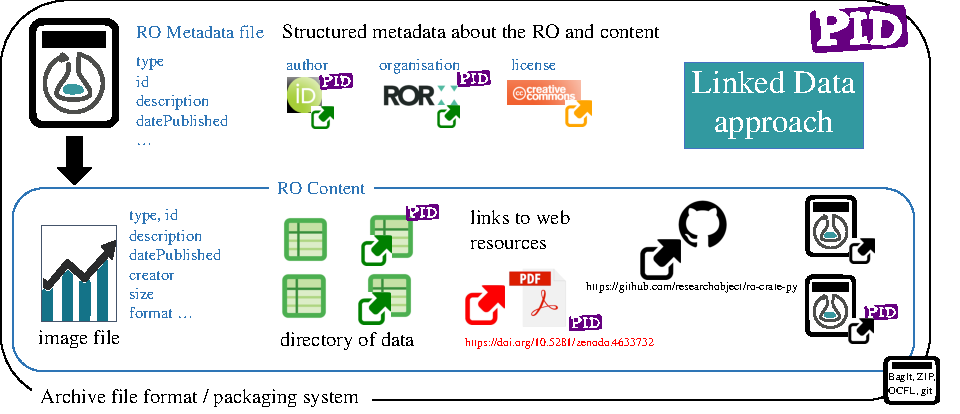
\includegraphics[width=\textwidth]{figures/ch05/ro-crate-overview.pdf}
	\caption[Conceptual overview of RO-Crate]{\textbf{Conceptual overview of RO-Crate}. A \emph{Persistent
  Identifier} (PID) \cite{McMurry 2017} points to a
  \emph{Research Object} (RO), which may be archived using different
  packaging approaches like BagIt \cite{ch5-74}, OCFL \cite
  {ch5-96}, git or ZIP. The RO is described within a \emph{RO-Crate
  Metadata File}, providing identifiers for \emph{authors} using ORCID,
  \emph{organisations} using Research Organization Registry (ROR) 
  \cite{ch5-79} and licences such as Creative Commons using SPDX
  identifiers. The \emph{RO-Crate content} is further described with
  additional metadata following a Linked Data approach. Data can be
  embedded files and directories, as well as links to external Web
  resources, PIDs and nested RO-Crates.}
  \label{ch5:fig:conceptual}
\end{figure}

\paragraph{Linked Data as a foundation}\label{ch5:linkeddata}

The \textbf{Linked Data} principles \cite{Bizer 2011}
(use of IRIs\footnote{\textbf{IRI}s \cite{Duerst 2005} are a generalisation
 of \textit{URI}s
(which include well-known http/https URLs), permitting international
Unicode characters without percent encoding, commonly used on the
browser address bar and in HTML5.} to identify resources (i.e. artefacts), resolvable via
HTTP, enriched with metadata and linked to each other) are core to
RO-Crate; therefore IRIs are used to identify an RO-Crate, its
constituent parts and metadata descriptions, and the properties and
classes used in the metadata.

RO-Crates are \emph{self-described} and follow the Linked Data
principles to describe all of their resources in both human and machine
readable manner. Hence, resources are identified using global
identifiers (absolute IRIs) where possible; and relationships between
two resources are defined with links.

The foundation of Linked Data and shared vocabularies also means that
multiple RO-Crates and other Linked Data resources can be indexed,
combined, queried, validated or transformed using existing Semantic Web
technologies such as SPARQL,\footnote{\url{https://www.w3.org/TR/sparql11-overview}}
SHACL\footnote{\url{https://www.w3.org/TR/shacl/}} and well established \textit{knowledge
graph} triple stores like Apache Jena\footnote{\url{https://jena.apache.org/}} and
OntoText GraphDB.\footnote{\url{https://www.ontotext.com/products/graphdb/}}

The possibilities of consuming\footnote{Some consideration is needed in processing of RO-Crates as
knowledge graphs, e.g. establishing absolute IRIs for files inside a
ZIP archive, detailed in the RO-Crate specification: \url
{https://www.researchobject.org/ro-crate/1.1/appendix/relative-uris.html}.} RO-Crate metadata with such
powerful tools gives another strong reason for using Linked Data as a
foundation. This use of mature Web\footnote{Note that an RO-Crate is not required to be published on the
Web, see Section~\vref{ch5:selfdescribed}.} technologies also means its
developers and consumers are not restricted to the Research Object
aspects that have already been specified by the RO-Crate community, but
can extend and integrate RO-Crate in multiple standardised ways.


\paragraph{RO-Crate is a self-described container}\label{ch5:selfdescribed}

An RO-Crate is defined\footnote{\url{https://www.researchobject.org/ro-crate/1.1/structure.html\#ro-crate-metadata-file-ro-crate-metadatajson}} as a self-described \textbf{Root Data Entity} that describes
and contains \emph{data entities}, which are further described by
referencing \emph{contextual entities}. A \textbf{data entity} is either
a \emph{file} (i.e.~a byte sequence stored on disk somewhere) or a
\emph{directory} (i.e.~set of named files and other directories). A file
does not need to be stored inside the RO-Crate root, it can be
referenced via a PID/IRI. A \textbf{contextual entity} exists outside
the information system (e.g.~a Person, a workflow language) and is
stored solely by its metadata. The representation of a \emph{data
entity} as a byte sequence makes it possible to store a variety of
research artefacts including not only data but also, for instance,
software and text.


The Root Data Entity is a directory, the \emph{RO-Crate Root},
identified by the presence of the \textbf{RO-Crate Metadata File}
\texttt{ro-crate-metadata.json} (top of Figure \vref{ch5:fig:conceptual}). This file describes the
RO-Crate using Linked Data, its content and related metadata using
Linked Data in JSON-LD format \cite{w3-ldp}. This
is a W3C standard RDF serialisation that has become popular; it is easy
to read by humans while also offering some advantages for data exchange
on the Internet. JSON-LD, a subset of the widely supported and
well-known JSON format, has tooling available for many programming languages.\footnote{\url{https://json-ld.org/\#developers}}

The minimal requirements for the root data entity
metadata\footnote{\url{https://www.researchobject.org/ro-crate/1.1/root-data-entity.html\#direct-properties-of-the-root-data-entity}}
are \texttt{name}, \texttt{description} and \texttt{datePublished}, as well as a contextual
entity identifying its \texttt{license} -- additional metadata are commonly
added to entities depending on the purpose of the particular RO-Crate.

RO-Crates can be stored, transferred or published in multiple ways,
e.g.~BagIt \cite{ch5-74}, Oxford
Common File Layout \cite{ch5-96} (OCFL),
downloadable ZIP archives in Zenodo or through dedicated online
repositories, as well as published directly on the Web, e.g.~using
GitHub Pages.\footnote{\url{https://pages.github.com/}} Combined with Linked Data identifiers, this caters for a diverse set of storage and access
requirements across different scientific domains, from metagenomics
workflows producing hundreds of gigabytes of genome data to cultural
heritage records with access restrictions for personally identifiable
data. Specific \emph{RO-Crate profiles} (Section~\vref{ch5:profiles}) may constrain serialization
and publication expectations, and require additional contextual types
and properties.

\paragraph{Data Entities are described using Contextual
Entities}\label{ch5:contextualentities}

RO-Crate distinguishes between data and contextual
entities\footnote{\url{https://www.researchobject.org/ro-crate/1.1/contextual-entities.html\#contextual-vs-data-entities}} in a similar way to HTTP terminology's early
attempt to separate \emph{information} (data) and \emph{non-information}
(contextual) resources \cite{ch5-120}. Data entities are usually files and directories located by relative IRI
references within the RO-Crate Root, but they can also be Web resources
or restricted data identified with absolute IRIs, including
\emph{Persistent Identifiers} (PIDs)
\cite{McMurry 2017}.

As both types of entities are identified by IRIs, their distinction is
allowed to be blurry; data entities can be located anywhere and be
complex, while contextual entities can have a Web presence beyond their
description inside the RO-Crate. For instance
\texttt{https://orcid.org/0000-0002-1825-0097} is primarily an
identifier for a person, but secondarily it is also a Web page and a way
to refer to their academic work.

A particular IRI may appear as a contextual entity in one RO-Crate and
as a data entity in another; the distinction lies in the fact that data
entities can be considered to be \emph{contained} or captured by that
RO-Crate (\textit{RO Content} in Figure \vref{ch5:fig:conceptual}), 
while contextual entities mainly \emph{explain} an RO-Crate or its
content (although this distinction is not a formal requirement).

In RO-Crate, a referenced contextual entity (e.g.~a person identified by
ORCID) should always be described within the RO-Crate Metadata File with
at least a \emph{type} and \emph{name}, even where their PID might
resolve to further Linked Data. This is so that clients are not required
to follow every link for presentation purposes, for instance HTML
rendering. Similarly any imported extension
terms\footnote{\url{https://www.researchobject.org/ro-crate/1.1/appendix/jsonld.html\#extending-ro-crate}} would themselves also have a human-readable description in the
case where their PID does not directly resolve to human-readable
documentation.

Figure \vref{ch5:fig:uml} shows a simplified UML class
diagram of RO-Crate, highlighting the different types of data entities
and contextual entities that can be aggregated and related. While an
RO-Crate would usually contain one or more data entities
(\texttt{hasPart}), it may also be a pure aggregation of contextual
entities (\texttt{mentions}).

\begin{figure}
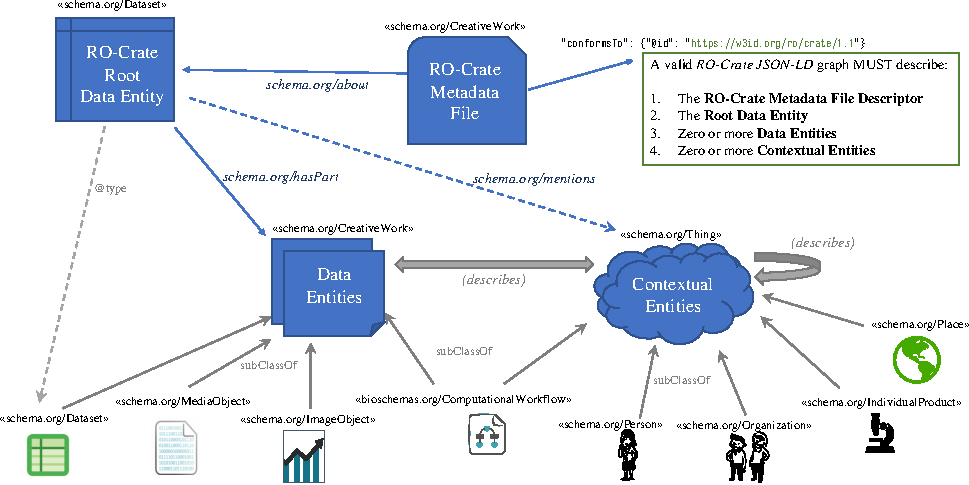
\includegraphics[width=\textwidth]{figures/ch05/ro-crate-uml.pdf}
	\caption[Simplified UML class diagram of RO-Crate]{\textbf{Simplified UML class diagram of RO-Crate}. The 
\emph{RO-Crate Metadata File} conforms to a version of the specification;
and contains a JSON-LD graph \cite{w3-ldp} that describes the
entities that make up the RO-Crate. The \emph{RO-Crate Root Data
Entity} represent the Research Object as a dataset. The RO-Crate
aggregates \emph{data entities} (\texttt{hasPart}) which are further
described using \emph{contextual entities} (which may include
aggregated and non-aggregated data entities). Multiple types and
relations from Schema.org allow annotations to be more specific,
including figures, nested datasets, computational workflows, people,
organisations, instruments and places. Contextual entities not
otherwise cross-referenced from other entities' properties 
(\emph{describes}) can be grouped under the root entity (\texttt{mentions}).}
\label{ch5:fig:uml}
\end{figure}

\paragraph{Guide through Recommended
Practices}\label{ch5:recommendedpractices}

RO-Crate as a specification aims to build a set of recommended practices
on how to practically apply existing standards in a common way to
describe research outputs and their provenance, without having to learn
each of the underlying technologies in detail.

As such, the RO-Crate 1.1
specification\footnote{\url{https://w3id.org/ro/crate/1.1}} \cite{rocrate1.1}
can be seen as an opinionated and example-driven guide to writing
\footurl{https://schema.org/}{Schema.org}
\cite{Guha 2015} metadata as
JSON-LD \cite{w3-ldp} (see
section \vref{ch5:implementation}), which
leaves it open for implementers to include additional metadata using
other Schema.org types and properties, or even additional Linked Data
vocabularies/ontologies or their own ad-hoc terms.

However the primary purpose of the RO-Crate specification is to assist
developers in leveraging Linked Data principles for the focused purpose
of describing Research Objects in a structured language, while reducing
the steep learning curve otherwise associated with Semantic Web
adaptation, like development of ontologies, identifiers, namespaces, and
RDF serialization choices.

\subsubsection{Ensuring Simplicity}\label{ch5:simplicity}

One aim of RO-Crate is to be conceptually simple. This simplicity has
been repeatedly checked and confirmed through an informal community
review process. For instance, in the discussion on supporting ad-hoc
vocabularies\footnote{\url{https://github.com/ResearchObject/ro-crate/issues/71}} in
RO-Crate, the community explored potential Linked Data solutions. The
conventional wisdom in RDF best
practices\footnote{\url{https://www.w3.org/TR/swbp-vocab-pub/}} is to establish a
vocabulary with a new IRI namespace, formalised using RDF
Schema\footnote{\url{http://www.w3.org/TR/2014/REC-rdf-schema-20140225/}} or
OWL\footnote{\url{http://www.w3.org/TR/2012/REC-owl2-overview-20121211/}}
ontologies. However, this may seem an excessive learning curve for
non-experts in semantic knowledge representation, and the RO-Crate
community instead agreed on a dual lightweight approach: (i)
Document\footnote{\url{https://www.researchobject.org/ro-crate/1.1/appendix/jsonld.html\#adding-new-or-ad-hoc-vocabulary-terms}}
how projects with their own Web-presence can make a pure HTML-based
vocabulary, and (ii) provide a community-wide PID namespace under
\texttt{https://w3id.org/ro/terms} that redirect to simple CSV files
maintained in GitHub.\footnote{\url{https://github.com/ResearchObject/ro-terms}}

To further verify this idea of simplicity, we have formalised the
RO-Crate definition (see \textit{section ~\vref{ch5:formaldefinition}}). An
important result of this exercise is that the underlying data structure
of RO-Crate, although conceptually a graph, is represented as a
depth-limited tree. This formalisation also emphasises the
\textit{boundedness} of the structure; namely, the fact that elements are
specifically identified as being either semantically \textit{contained} by the
RO-Crate as \textit{Data Entities} (\texttt{hasPart}) or mainly referenced
(\texttt{mentions}) and typed as \textit{external} to the Research Object as
\textit{Contextual Entities}. It is worth pointing out that this semantic
containment can extend beyond the physical containment of files
residing within the RO-Crate Root directory on a given storage system,
as the RO-Crate data entities may include any data resource globally
identifiable using IRIs.

\subsubsection{Extensibility and RO-Crate profiles}\label{ch5:profiles}

The RO-Crate specification provides a core set of conventions to
describe research outputs using types and properties applicable across
scientific domains. However we have found that domain-specific use of
RO-Crate will, implicitly or explicitly, form a specialised
\textbf{profile} of RO-Crate; i.e., \emph{a set of conventions, types
and properties that are minimally required and one can expect to be
present in that subset of RO-Crates}. For instance, RO-Crates used for
exchange of workflows will have to contain a data entity of type
\texttt{ComputationalWorkflow}, or cultural heritage records should have
a \texttt{contentLocation}.

Making such profiles explicit allow further reliable programmatic
consumption and generation of RO-Crates beyond the core types defined in
the RO-Crate specification. Following the RO-Crate mantra of
\emph{guidance over strictness}, profiles are mainly \emph{duck-typing}
rather than strict syntactic or semantic types, but may also have
corresponding machine-readable schemas at multiple levels (file formats,
JSON, RDF shapes, RDFS/OWL semantics).

The next version of the RO-Crate specification 1.2 will define a
formalization\footnote{\url{https://www.researchobject.org/ro-crate/1.2-DRAFT/profiles}}
for publishing and declaring conformance to RO-Crate profiles. Such a
profile is primarily a human-readable document of before-mentioned
expectations and conventions, but may also define a machine-readable
profile as a \textbf{Profile Crate}: Another RO-Crate that describe the
profile and in addition can list schemas for validation, compatible
software, applicable repositories, serialization/packaging formats,
extension vocabularies, custom JSON-LD contexts and examples (see for
example the Workflow RO-Crate
profile\footnote{\url{https://w3id.org/workflowhub/workflow-ro-crate/}}).


In addition, there are sometimes existing domain-specific metadata
formats, but they are either not RDF-based (and thus time-consuming to
construct terms for in JSON-LD) or are at a different granularity level
that might become overwhelming if represented directly in the RO-Crate
Metadata file (e.g.~W3C PROV bundle detailing every step execution of a
workflow run
\cite{Khan 2019}). RO-Crate
allows such \emph{alternative metadata files} to co-exist, and be
described as data entities with references to the standards and
vocabularies they conform to. This simplifies further programmatic
consumption even where no filename or file extension conventions have
emerged for those metadata formats.

Section \vref{ch5:inuse} examines the observed
specializations of RO-Crate use in several domains and their emerging
profiles.

\subsubsection{Technical implementation of the RO-Crate
model}\label{ch5:implementation}

The RO-Crate conceptual model has been realised using JSON-LD and
Schema.org in a prescriptive form as discussed in Section~\vref{ch5:conceptual}. These technical
choices were made to cater for simplicity from a developer perspective
(as introduced in Section~\vref{ch5:methodology}).

JSON-LD\footnote{\url{https://json-ld.org/}} \cite{w3-ldp}
provides a way to express Linked Data as a JSON structure, where a
\emph{context} provides mapping to RDF properties and classes. While
JSON-LD cannot map arbitrary JSON structures to RDF, we found that it
does lower the barrier compared to other RDF syntaxes, as the JSON
syntax nowadays is a common and popular format for data exchange on the
Web.

However, JSON-LD alone has too many degrees of freedom and hidden
complexities for software developers to reliably produce and consume
without specialised expertise or large RDF software frameworks. A large
part of the RO-Crate specification is therefore dedicated to describing
the acceptable subset of JSON structures.

\paragraph{RO-Crate JSON-LD}\label{ch5:jsonld}

RO-Crate
mandates\footnote{\url{https://www.researchobject.org/ro-crate/1.1/appendix/jsonld.html}}
the use of flattened, compacted JSON-LD in the RO-Crate Metadata file
\texttt{ro-crate-metadata.json}\footnote{The avid reader may spot that the RO-Crate Metadata file use the
extension \texttt{.json} instead of \texttt{.jsonld}, this is to emphasise the
developer expectations as a JSON format, while the file's JSON-LD
nature is secondary. See \url
{https://github.com/ResearchObject/ro-crate/issues/82}.}
where a single \texttt{@graph} array contains all
the data and contextual entities in a flat list. An example can be seen
in the JSON-LD snippet in Listing \vref{ch5:lis1}, describing a simple RO-Crate
containing data entities described using contextual entities.

\begin{listing}
  \footnotesize
  \begin{verbatim}
  { "@context": "https://w3id.org/ro/crate/1.1/context",
    "@graph": [
      { "@id": "ro-crate-metadata.json",      
        "@type": "CreativeWork",
        "conformsTo": {"@id": "https://w3id.org/ro/crate/1.1"},
        "about": {"@id": "./"}
      },
      { "@id": "./",
        "@type": "Dataset",
        "name": "A simplified RO-Crate",
        "author": {"@id": "#alice"},
        "license": {"@id": "https://spdx.org/licenses/CC-BY-4.0"},
        "datePublished": "2021-11-02T16:04:43Z",
        "hasPart": [
          {"@id": "survey-responses-2019.csv"},
          {"@id": "https://example.com/pics/5707039334816454031_o.jpg"}
        ]
      },
      { "@id": "survey-responses-2019.csv",
        "@type": "File",
        "about": {"@id": "https://example.com/pics/5707039334816454031_o.jpg"},
        "author": {"@id": "#alice"}
      },
      { "@id": "https://example.com/pics/5707039334816454031_o.jpg",
        "@type": ["File", "ImageObject"],
        "contentLocation": {"@id": "http://sws.geonames.org/8152662/"},
        "author": {"@id": "https://orcid.org/0000-0002-1825-0097"}
      },
      { "@id": "#alice",
        "@type": "Person",
        "name": "Alice"
      },
      { "@id": "https://orcid.org/0000-0002-1825-0097",
        "@type": "Person",
        "name": "Josiah Carberry"
      },
      { "@id": "http://sws.geonames.org/8152662/",
        "@type": "Place",
        "name": "Catalina Park"
      },
      { "@id": "https://spdx.org/licenses/CC-BY-4.0",
        "@type": "CreativeWork",
        "name": "Creative Commons Attribution 4.0"
      }
    ]
  }    
  \end{verbatim}    
	\caption[Simplified RO-Crate metadata file]{%\qq{}\protect\footnotemark[31]
  Simplified\footnotemark RO-Crate metadata file showing the
  flattened compacted JSON-LD \texttt{@graph} array containing the data entities
  and contextual entities, cross-referenced using \texttt{@id}. The
  \texttt{ro-crate-metadata.json} entity self-declares conformance with the
  RO-Crate specification using a versioned persistent identifier, further
  RO-Crate descriptions are on the root data entity \texttt{./} or any of the
  referenced data or contextual entities. This is exemplified by the data
  entity \texttt{ImageObject} referencing contextual entities for
  \texttt{contentLocation} and \texttt{author} that differs from that of the overall
  RO-Crate. In this crate, \texttt{about} of the CSV data entity reference the
  \texttt{ImageObject}, which then take the roles of both a data entity and
  contextual entity. While \texttt{Person} entities ideally are identified with
  ORCID PIDs as for Josiah, \texttt{\#alice} is here in contrast an RO-Crate
  local identifier, highlighting the pragmatic ``just enough'' Linked
  Data approach.}
  \label{ch5:lis1}
\end{listing}
  
\footnotetext{
    Recommended properties for types shown in
    listing also include
    \texttt{affiliation}, \texttt{citation}, \texttt{contactPoint},
    \texttt{description},
    \texttt{encodingFormat}, \texttt{funder}, \texttt{geo}, \texttt{identifier},
    \texttt{keywords},
    \texttt{publisher}; these properties and corresponding contextual
    entities are
    excluded here for brevity. See complete example
    \url
    {https://www.researchobject.org/2021-packaging-research-artefacts-with-ro-crate/listing1/}.
}
 

In this flattened profile of JSON-LD, each \texttt{\{entity\}} are
directly under \texttt{@graph} and represents the RDF triples with a
common \emph{subject} (\texttt{@id}), mapped \emph{properties} like
\texttt{hasPart}, and \emph{objects} --- as either literal
\texttt{"string"} values, referenced \texttt{\{objects\}} (which
properties are listed in its own entity), or a JSON \texttt{{[}list{]}}
of these. If processed as JSON-LD, this forms an RDF graph by matching
the \texttt{@id} IRIs and applying the \texttt{@context} mapping to
Schema.org terms. \normalsize

\paragraph{Flattened JSON-LD}\label{ch5:flattened-json-ld}

When JSON-LD 1.0 \cite{w3-ldp}
was
proposed, one of the motivations was to seamlessly apply an RDF nature
on top of regular JSON as frequently used by Web APIs. JSON objects in
APIs are frequently nested with objects at multiple levels, and the
perhaps most common form of JSON-LD is the compacted
form\footnote{\url{https://json-ld.org/spec/REC/json-ld/20140116/\#compacted-document-form}}
which follows this expectation (JSON-LD
1.1\footnote{\url{https://www.w3.org/TR/2020/REC-json-ld11-20200716/}} further
expands these capabilities, e.g. allowing nested \texttt{@context} definitions).


While this feature of JSON-LD can be seen as a way to ``hide'' its RDF
nature, we found that the use of nested trees (e.g.~a \texttt{Person}
entity appearing as \texttt{author} of a \texttt{File} which nests under
a \texttt{Dataset} with \texttt{hasPart}) counter-intuitively forces
consumers to consider the JSON-LD as an RDF Graph, since an identified
\texttt{Person} entity can appear at multiple and repeated points of the
tree (e.g.~author of multiple files), necessitating node merging or
duplication, which can become complicated as this approach also invites
the use of \emph{blank nodes} (entities missing \texttt{@id}).

By comparison, a single flat \texttt{@graph} array approach, as required
by RO-Crate, means that applications can choose to process and edit each
entity as pure JSON by a simple lookup based on \texttt{@id}. At the
same time, lifting all entities to the same level reflects the Research
Object principles
\cite{Bechhofer 2013}
in that describing the context and provenance is just as important as
describing the data, and the requirement of \texttt{@id} of every entity
forces RO-Crate generators to consciously
consider
existing IRIs and identifiers.\footnote{\url{https://www.researchobject.org/ro-crate/1.1/appendix/jsonld.html\#describing-entities-in-json-ld}}

\paragraph{JSON-LD context}\label{ch5:json-ld-context}

In JSON-LD, the \texttt{@context} is a reference to another JSON-LD
document that provides mapping from JSON keys to Linked Data term IRIs,
and can enable various JSON-LD directives to cater for customised JSON
structures for translating to RDF.

RO-Crate reuses vocabulary terms and IRIs from Schema.org, but provides
its own versioned JSON-LD
context,\footnote{\url{https://w3id.org/ro/crate/1.1/context}} which has a flat list
with the mapping from JSON-LD keys to their IRI equivalents (e.g. key
\texttt{"author"} maps to the \url{http://schema.org/author} property).

The rationale behind this decision is to support JSON-based RO-Crate
applications that are largely unaware of JSON-LD, that still may want to
process the \texttt{@context} to find or add Linked Data definitions of
otherwise unknown properties and types. Not reusing the official
Schema.org context means RO-Crate is also able to map in additional
vocabularies where needed, namely the \emph{Portland Common Data Model}
(PCDM) \cite{Cossu 2018}
for
repositories and Bioschemas \cite{Gray 2017}
for
describing computational workflows. RO-Crate profiles may
extend\footnote{\url{https://www.researchobject.org/ro-crate/1.1/appendix/jsonld.html\#extending-ro-crate}}
the \texttt{@context} to re-use additional domain-specific ontologies.


Similarly, while the Schema.org context
currently\footnote{\url{https://schema.org/version/13.0/schemaorg-current-http.jsonld}}
have \texttt{"@type": "@id"} annotations for implicit object properties, RO-Crate
JSON-LD distinguishes explicitly between references to other entities
\texttt{\{"@id": "\#alice"}\}
and string values \texttt{"Alice"} -- meaning
RO-Crate applications can find references for corresponding entities
and IRIs without parsing the \texttt{@context} to understand a particular
property. Notably this is exploited by the \textit{ro-crate-html-js}
\cite{ch5-95} tool to provide reliable HTML rendering for
otherwise unknown properties and types.

\subsubsection{RO-Crate Community}\label{ch5:community}

The RO-Crate conceptual model, implementation and best practices are
developed by a growing community of researchers, developers and
publishers. RO-Crate's community is a key aspect of its effectiveness in
making research artefacts FAIR. Fundamentally, the community provides
the overall context of the implementation and model and ensures its
interoperability.

The RO-Crate community consists of:

\begin{enumerate}
\item
  a diverse set of people representing a variety of stakeholders;
\item
  a set of collective norms;
\item
  an open platform that facilitates communication (GitHub, Google Docs,
  monthly teleconferences).
\end{enumerate}

\hypertarget{people}{%
\paragraph{People}\label{ch5:people}}

The initial concept of RO-Crate was formed at the first Workshop on
Research Objects\footnote{\url{https://www.researchobject.org/ro2018/}} (RO2018),
held as part of the IEEE conference on eScience. This workshop followed
up on considerations made at a Research Data Alliance (RDA) meeting on
Research Data
Packaging\footnote{\url{https://rd-alliance.org/approaches-research-data-packaging-rda-11th-plenary-bof-meeting}}
that found similar goals across multiple data packaging efforts
\cite{OCarragain 2019}: simplicity, structured metadata and the
use of JSON-LD.

An important outcome of discussions that took place at RO2018 was the
conclusion that the original Wf4Ever Research Object ontologies
\cite{Belhajjame 2015}, in
principle sufficient for packaging research artefacts with rich
descriptions, were, in practice, considered inaccessible for regular
programmers (e.g., Web developers) and in danger of being
incomprehensible for domain scientists due to their reliance on Semantic
Web technologies and other ontologies.

DataCrate \cite{ch5-103} was
presented at RO2018 as a promising lightweight alternative approach, and
an agreement was made by a group of volunteers to attempt building what
was initially called \emph{``RO Lite''} as a combination of DataCrate's
implementation and Research Object's principles.

This group, originally made up of library and Semantic Web experts, has
subsequently grown to include domain scientists, developers, publishers
and more. This perspective of multiple views led to the specification
being used in a variety of domains, from bioinformatics and regulatory
submissions to humanities and cultural heritage preservation.

The RO-Crate community is strongly engaged with the European-wide
biology/bioinformatics collaborative e-Infrastructure ELIXIR
\cite{Crosswell 2012}, along with European Open Science
Cloud\footnote{\url{https://eosc.eu/}} (EOSC) projects including
EOSC-Life,\footnote{\url{https://www.eosc-life.eu/}}
FAIRplus,\footnote{\url{https://fairplus-project.eu/}}
CS3MESH4EOSC\footnote{\url{https://cs3mesh4eosc.eu/}} and
BY-COVID.\footnote{\url{https://by-covid.eu/}} RO-Crate has also established
collaborations with Bioschemas \cite{Gray 2017}, GA4GH
\cite{Rehm 2021}, OpenAIRE \cite{ch5-100}
and multiple H2020 projects.

A key set of stakeholders are developers: the RO-Crate community has
made a point of attracting developers who can implement the
specifications but, importantly, keeps ``developer user experience'' in
mind. This means that the specifications are straightforward to
implement and thus do not require expertise in technologies that are not
widely deployed.

This notion of catering to ``developer user experience'' is an example
of the set of norms that have developed and now define the community.

\paragraph{Norms}\label{ch5:norms}

The RO-Crate community is driven by informal conventions and notions
that are prevalent but not neccessarily written down. Here, we distil
what we as authors believe are the critical set of norms that have
facilitated the development of RO-Crate and contributed to the ability
for RO-Crate research packages to be FAIR. This is not to say that there
are no other norms within the community nor that everyone in the
community holds these uniformly. Instead, what we emphasise is that
these norms are helpful and also shaped by community practices.

\begin{enumerate}
\item
  Simplicity
\item
  Developer friendliness
\item
  Focus on examples and best practices rather than rigorous
  specification
\item
  Reuse ``just enough'' Web standards
\end{enumerate}

A core norm of RO-Crate is that of \textbf{simplicity}, which sets the
scene for how we guide developers to structure metadata with RO-Crate.
We focus mainly on documenting simple approaches to the most common use
cases, such as authors having an affiliation. This norm also influences
our take on \textbf{developer friendliness}; for instance, we are using
the Web-native JSON format, allowing only a few of JSON-LD's flexible
Linked Data features. Moreover, the RO-Crate documentation is largely
built up by \textbf{examples} showcasing \textbf{best practices}, rather
than rigorous specifications. We build on existing \textbf{Web
standards} that themselves are defined rigorously, which we utilise
\emph{``\textbf{just enough}''} in order to benefit from the advantages
of Linked Data (e.g., extensions by namespaced vocabularies), without
imposing too many developer choices or uncertainties (e.g., having to
choose between the many RDF syntaxes).

While the above norms alone could easily lead to the creation of ``yet
another'' JSON format, we keep the goal of \textbf{FAIR
interoperability} of the captured metadata, and therefore follow closely
FAIR best practices and current developments such as data citations,
PIDs, open repositories and recommendations for sharing research outputs
and software.

\paragraph{Open Platforms}\label{ch5:open-platforms}

The critical infrastructure that enables the community around RO-Crate
is the use of open development platforms. This underpins the importance
of open community access to supporting FAIR. Specifically, it is
difficult to build and consume FAIR research artefacts without being
able to access the specifications, understand how they are developed,
know about any potential implementation issues, and discuss usage to
evolve best practices.

The development of RO-Crate was driven by capturing documentation of
real-life examples and best practices rather than creating a rigorous
specification. At the same time, we agreed to be opinionated on the
syntactic form to reduce the jungle of implementation choices; we wanted
to keep the important aspects of Linked Data to adhere to the FAIR
principles while retaining the option of combining and extending the
structured metadata using the existing Semantic Web stack, not just
build a standalone JSON format.

Further work during 2019 started adapting the DataCrate documentation
through a more collaborative and exploratory \emph{RO Lite} phase,
initially using Google Docs for review and discussion, then moving to
GitHub as a collaboration space for developing what is now the RO-Crate
specification, maintained\footnote{\url{https://github.com/researchobject/ro-crate/}} as
Markdown in GitHub Pages
and published through Zenodo.

In addition to the typical Open Source-style development with GitHub
issues and pull requests, the RO-Crate Community have, at time of
writing, two regular monthly calls, a Slack channel and a mailing list
for coordinating the project; also many of its participants collaborate
on RO-Crate at multiple conferences and coding events such as the
ELIXIR BioHackathon.\footnote{\url{https://biohackathon-europe.org/}} The community
is jointly developing the RO-Crate specification and Open Source tools,
as well as providing support and considering new use cases. The
RO-Crate Community\footnote{\url{https://www.researchobject.org/ro-crate/community}}
is open for anyone to join, to equally participate under a code of
conduct, and as of October 2021 has more than 50 members (see \vref{ro-crate-community}).

\subsection{RO-Crate Tooling}\label{ch5:tooling}

The work of the community has led to the development of a number of
tools for creating and using RO-Crates. Table \vref{ch5:tab1} shows the current set
of implementations. Reviewing this list, one can see support for
commonly used programming languages, including Python, JavaScript, and
Ruby. Additionally, the tools can be integrated into commonly used
research environments, in particular, the command line tool
\textit{ro-crate-html-js} \cite{ch5-95} for creating a human-readable
preview of an RO-Crate as a sidecar HTML file. Furthermore, there are
tools that cater to end-users (\textit{Describo} \cite{ch5-78}, \textit{WorkflowHub}
\cite{ch5-124}), in order to simplify creating and managing
RO-Crate. For example, Describo was developed to help researchers of
the Australian Criminal Characters
project\footnote{\url{https://criminalcharacters.com/}} to annotate historical prisoner
records for greater insight into the history of Australia
\cite{ch5-97}.

While the development of these tools is promising, our analysis of their
maturity status shows that the majority of them are in the Beta stage.
This is partly due to the fact that the RO-Crate specification itself
only recently reached 1.0 status, in November 2019
\cite{ch5-105}. Now that there
is a fixed point of reference: With version 1.1 (October 2020)
\cite{ch5-107} RO-Crate has
stabilised based on feedback from application development, and now we
are seeing a further increase in the maturity of these tools, along with
the creation of new ones.

Given the stage of the specification, these tools have been primarily
targeting developers, essentially providing them with the core libraries
for working with RO-Crate. Another target has been that of research data
managers who need to manage and curate large amounts of data.

\small
\begin{longtable}[]{@{}
  >{\raggedright\arraybackslash}p{(\columnwidth - 8\tabcolsep) * \real{0.21}}
  >{\raggedright\arraybackslash}p{(\columnwidth - 8\tabcolsep) * \real{0.11}}
  >{\raggedright\arraybackslash}p{(\columnwidth - 8\tabcolsep) * \real{0.19}}
  >{\raggedright\arraybackslash}p{(\columnwidth - 8\tabcolsep) * \real{0.09}}
  >{\raggedright\arraybackslash}p{(\columnwidth - 8\tabcolsep) * \real{0.40}}@{}}
\toprule
Tool Name & Targets & Language /Platform & Status & Brief Description \\
\midrule
\endhead
Describo \cite{ch5-78} &
Research Data Managers & NodeJS (Desktop) & RC & Interactive desktop
application to create, update and export RO-Crates for different
profiles \\
Describo Online
\cite{ch5-77} &
Platform developers & NodeJS (Web) & Alpha & Web-based application to
create RO-Crates using cloud storage \\
ro-crate-excel
\cite{ch5-84} & Data
managers & JavaScript & Beta & Command-line tool to create/edit
RO-Crates with spreadsheets \\
ro-crate-html-js
\cite{ch5-95} &
Developers & JavaScript & Beta & HTML rendering of RO-Crate \\
ro-crate-js
\cite{ch5-49} & Research
Data Managers & JavaScript & Alpha & Library for creating/manipulating
crates; basic validation code \\
ro-crate-ruby
\cite{Bacall 2022b} &
Developers & Ruby & Beta & Ruby library for reading/writing RO-Crate,
with workflow support \\
ro-crate-py \cite{ro-crate-py}) &
Developers & Python & Alpha & Object-oriented Python library for
reading/writing RO-Crate and use by Jupyter Notebook \\
WorkflowHub \cite{ch5-124} & Workflow
users & Ruby & Beta & Workflow repository; imports and exports Workflow
RO-Crate \\
Life Monitor \cite{CRS4 2022} & Workflow
developers & Python & Alpha & Workflow testing and monitoring service;
Workflow Testing profile of RO-Crate \\
SCHeMa \cite{ch5-118} & Workflow
users & PHP & Alpha & Workflow execution using RO-Crate as exchange
mechanism
\cite{10.5281/zenodo.4671709} \\
galaxy2cwl \cite{ch5-50}
& Workflow developers & Python & Alpha & Wraps Galaxy workflow as
Workflow RO-Crate \\
Modern PARADISEC \cite{ch5-51} &
Repository managers & Platform & Beta & Cultural Heritage portal based
on OCFL and RO-Crate \\
ONI express
\cite{Arkisto 2022} &
Repository managers & Platform & Beta & Platform for publishing data and
documents stored in an OCFL repository via a Web interface \\
ocfl-tools \cite{ch5-52} &
Developers & JavaScript (CLI) & Beta & Tools for managing RO-Crates in
an OCFL repository \\
RO Composer
\cite{Bacall 2019} &
Repository developers & Java & Alpha & REST API for gradually building
ROs for given profile. \\
RDA maDMP Mapper \cite{Arfaoui 2020}
& Data Management Plan users & Python & Beta & Mapping between
machine-actionable data management plans (maDMP) and RO-Crate
\cite{Miksa 2020} \\
Ro-Crate\_2\_ma-DMP
\cite{Brenner 2020} & Data
Management Plan users & Python & Beta & Convert between
machine-actionable data management plans (maDMP) and RO-Crate \\
CheckMyCrate
\cite{Belchev 2021} &
Developers & Python (CLI) & Alpha & Validation according to Workflow
RO-Crate profile \\
RO-Crates-and-Excel
\cite{ch5-126} & Data Managers
& Java (CLI) & Alpha & Describe column/data details of spreadsheets as
RO-Crate using DataCube vocabulary \\
\bottomrule
\caption[Applications and libraries implementing RO-Crate]{Applications and libraries implementing RO-Crate, targeting
  different types of users across multiple programming languages. Status
  is indicative as assessed by this work (Alpha \textless{} Beta
  \textless{} Release Candidate (RC) \textless{} Release).
}
\label{ch5:tab1}
\end{longtable}

\normalsize


\subsection{Profiles of RO-Crate in use}\label{ch5:inuse}

RO-Crate fundamentally forms part of an infrastructure to help build
FAIR research artefacts. In other words, the key question is whether
RO-Crate can be used to share and (re)use research artefacts. Here we
look at three research domains where RO-Crate is being applied:
Bioinformatics, Regulatory Science and Cultural Heritage. In addition,
we note how RO-Crate may have an important role as part of
machine-actionable data management plans and institutional repositories.

From these varied uses of RO-Crate we observe natural differences in
their detail level and the type of entities described by the RO-Crate.
For instance, on submission of an RO-Crate to a workflow repository, it
is reasonable to expect the RO-Crate to contain at least one workflow,
ideally with a declared licence and workflow language. Specific
additional recommendations such as on identifiers is also needed to meet
the emerging requirements of FAIR Digital
Objects.\footnote{\url{https://fairdo.org/}} Work has now
begun\footnote{\url{https://github.com/ResearchObject/ro-crate/issues/153}} to
formalise these different \textit{profiles} of RO-Crates, which may impose
additional constraints based on the needs of a specific domain or use case.


\subsubsection{Bioinformatics workflows}\label{ch5:workflows}

WorkflowHub.eu\footnote{\url{https://workflowhub.eu/}} is a European cross-domain
registry of computational workflows, supported by European Open Science
Cloud projects, e.g. EOSC-Life,\footnote{\url{https://www.eosc-life.eu/}} and
research infrastructures including the pan-European bioinformatics
network ELIXIR\footnote{\url{https://elixir-europe.org/}}
\cite{Crosswell 2012}. As part
of promoting workflows as reusable tools, WorkflowHub includes
documentation and high-level rendering of the workflow structure
independent of its native workflow definition format. The rationale is
that a domain scientist can browse all relevant workflows for their
domain, before narrowing down their workflow engine requirements. As
such, the WorkflowHub is intended largely as a registry of workflows
already deposited in repositories specific to particular workflow
languages and domains, such as UseGalaxy.eu
\cite{Baker 2020} and
Nextflow nf-core
\cite{Ewels 2020}.

We here describe three different RO-Crate profiles developed for use
with WorkflowHub.

\paragraph{Profile for describing workflows}
\label{ch5:profile-for-describing-workflows}

Being cross-domain, WorkflowHub has to cater for many different workflow
systems. Many of these, for instance Nextflow
\cite{Di Tommaso 2017} and Snakemake
\cite{Koster 2012}, by
virtue of their script-like nature, reference multiple neighbouring
files typically maintained in a GitHub repository. This calls for a data
exchange method that allows keeping related files together. WorkflowHub
has tackled this problem by adopting RO-Crate as the packaging mechanism
\cite{Bietrix 2021}, typing and
annotating the constituent files of a workflow and --- crucially ---
marking up the workflow language, as many workflow engines use common
file extensions like \texttt{*.xml} and \texttt{*.json}. Workflows are
further described with authors, license, diagram previews and a listing
of their inputs and outputs. RO-Crates can thus be used for
interoperable deposition of workflows to WorkflowHub, but are also used
as an archive for downloading workflows, embedding metadata registered
with the WorkflowHub entry and translated workflow files such as
abstract Common Workflow Language (CWL)
\cite{Crusoe 2022} definitions and
diagrams \cite{Goble 2021}.

RO-Crate acts therefore as an interoperability layer between registries,
repositories and users in WorkflowHub. The iterative development between
WorkflowHub developers and the RO-Crate community heavily informed the
creation of the Bioschemas
\cite{Gray 2017} profile for Computational
Workflows \footnote{\url{https://bioschemas.org/profiles/ComputationalWorkflow/1.0-RELEASE/}}, which again informed the
RO-Crate
1.1 specification on workflows \footnote{\url{https://www.researchobject.org/ro-crate/1.1/workflows.html}} and led to the RO-Crate Python library
\cite{ro-crate-py} and
WorkflowHub's
\textbf{Workflow
RO-Crate profile}\footnote{\url{https://w3id.org/workflowhub/workflow-ro-crate/1.0}}, which, in a similar fashion to RO-Crate itself,
recommends which workflow resources and descriptions are required. This
co-development across project boundaries exemplifies the drive for
simplicity and for establishing best practices.

\paragraph{Profile for recording workflow runs}
\label{ch5:profile-for-recording-workflow-runs}

RO-Crates in WorkflowHub have so far been focused on workflows that are
ready to be run, and development of WorkflowHub is now creating a
\textbf{Workflow Run RO-Crate profile} for the purposes of benchmarking,
testing and executing workflows. As such, RO-Crate serves as a container
of both a \emph{workflow definition} that may be executed and of a
particular \emph{workflow execution with test results}.

This workflow run profile is a continuation of our previous work with
capturing workflow provenance in a Research Object in CWLProv
\cite{Khan 2019} and
TavernaPROV \cite{ch5-110}.
In both cases, we used the PROV Ontology
\cite{w3-prov-o},
including details of every task execution with all the intermediate
data, which required significant workflow engine integration.\footnote{CWLProv
  and TavernaProv predate RO-Crate, but use RO-Bundle
  \cite{ch5-111}, a similar
  Research Object packaging method with JSON-LD metadata.}

Simplifying from the CWLProv approach, the planned Workflow Run RO-Crate
profile will use a high level Schema.org
provenance\footnote{\url{https://www.researchobject.org/ro-crate/1.1/provenance.html\#software-used-to-create-files}}
for the input/output boundary of the overall workflow
execution. This \emph{Level 1 workflow provenance}
\cite{Khan 2019} can be
expressed generally across workflow languages with minimal workflow
engine changes, with the option of more detailed provenance traces as
separate PROV artefacts in the RO-Crate as data entities. In the current
development of Specimen Data
Refinery\footnote{\url{https://github.com/DiSSCo/SDR}} \cite{Walton 2020} these
RO-Crates will document the text recognition workflow runs of digitised
biological specimens, exposed as FAIR Digital Objects
\cite{De Smedt 2020}.

WorkflowHub has recently enabled minting of Digital Object Identifiers
(DOIs), a PID commonly used for scholarly artefacts, for registered
workflows, e.g.~\texttt{10.48546/workflowhub.workflow.56.1}
\cite{ch5-83},
lowering the barrier for citing workflows as computational methods along
with their FAIR metadata -- captured within an RO-Crate. While it is not
an aim for WorkflowHub to be a repository of workflow runs and their
data, RO-Crates of \emph{exemplar workflow runs} serve as useful
workflow documentation, as well as being an exchange mechanism that
preserves FAIR metadata in a diverse workflow execution environment.

\paragraph{Profile for testing workflows}\label{ch5:profile-for-testing-workflows}

The value of computational workflows, however, is potentially undermined
by the ``collapse'' over time of the software and services they depend
upon: for instance, software dependencies can change in a
non-backwards-compatible manner, or active maintenance may cease; an
external resource, such as a reference index or a database query
service, could shift to a different URL or modify its access protocol;
or the workflow itself may develop hard-to-find bugs as it is updated.
This \emph{workflow decay} can take a big toll on the workflow's
reusability and on the reproducibility of any processes it evokes
\cite{ch5-125}.

For this reason, WorkflowHub is complemented by a monitoring and testing
service called LifeMonitor
\cite{CRS4 2022}, also supported
by EOSC-Life. LifeMonitor's main goal is to assist in the creation,
periodic execution and monitoring of workflow tests, enabling the early
detection of software collapse in order to minimise its detrimental
effects. The communication of metadata related to workflow testing is
achieved through the adoption of a \textbf{Workflow Testing RO-Crate
profile}\footnote{\url{https://lifemonitor.eu/workflow_testing_ro_crate}} stacked on
top of the \textit{Workflow RO-Crate} profile. This further specialisation of
Workflow RO-Crate allows to specify additional testing-related entities
(test suites, instances, services, etc.), leveraging RO-Crate's
extension
mechanism\footnote{\url{https://www.researchobject.org/ro-crate/1.1/appendix/jsonld.html\#extending-ro-crate}}
through the addition of terms from custom namespaces.

In addition to showcasing RO-Crate's extensibility, the testing profile
is an example of the format's flexibility and adaptability to the
different needs of the research community. Though ultimately related to
a computational workflow, in fact, most of the testing-specific entities
are more about describing a protocol for interacting with a monitoring
service than a set of research outputs and its associated metadata.
Indeed, one of LifeMonitor's main functionalities is monitoring and
reporting on test suites running on existing Continuous Integration (CI)
services, which is described in terms of service URLs and job
identifiers in the testing profile. In principle, in this context, data
could disappear altogether, leading to an RO-Crate consisting entirely
of contextual entities. Such an RO-Crate acts more as an exchange format
for communication between services (WorkflowHub and LifeMonitor) than as
an aggregator for research data and metadata, providing a good example
of the format's high versatility.

\subsubsection{Regulatory Sciences}\label{ch5:regulatorysciences}

BioCompute Objects\footnote{\url{https://biocomputeobject.org/}} (BCO)
\cite{Alterovitz 2018} is a
community-led effort to standardise submissions of computational
workflows to biomedical regulators. For instance, a genomics sequencing
pipeline, as part of a personalised cancer treatment study, can be
submitted to the US Food and Drugs Administration (FDA) for approval.
BCOs are formalised in the standard IEEE 2791-2020
\cite{ieee2791}
as a combination of JSON
Schemas\footnote{\url{https://w3id.org/ieee/ieee-2791-schema/}}
that define the structure of JSON metadata files describing
exemplar workflow runs in detail, covering aspects such as the usability
and error domain of the workflow, its runtime requirements, the
reference datasets used and representative output data produced.

BCOs provide a structured view over a particular workflow, informing
regulators about its workings independently of the underlying workflow
definition language. However, BCOs have only limited support for
additional metadata.\footnote{IEEE 2791-2020 do permit user extensions
  in the \emph{extension domain} by referencing additional JSON Schemas.}
For instance, while the BCO itself can indicate authors and
contributors, and in particular regulators and their review decisions,
it cannot describe the provenance of individual data files or workflow
definitions.

As a custom JSON format, BCOs cannot be extended with Linked Data
concepts, except by adding an additional top-level JSON object
formalised in another JSON Schema. A BCO and workflow submitted by
upload to a regulator will also frequently consist of multiple
cross-related files. Crucially, there is no way to tell whether a given
\texttt{*.json} file is a BCO file, except by reading its content and
check for its \texttt{spec\_version}.

We can then consider how a BCO and its referenced artefacts can be
packaged and transferred following FAIR principles.
\textbf{BCO RO-Crate}\footnote{\url{https://biocompute-objects.github.io/bco-ro-crate/}} \cite{Soiland-Reyes 2021},
part of the BioCompute Object user guides, defines a set of best
practices for wrapping a BCO with a workflow, together with its exemplar
outputs in an RO-Crate, which then provides typing and additional
provenance metadata of the individual files, workflow definition,
referenced data and the BCO metadata itself.

Here the BCO is responsible for describing the \emph{purpose} of a
workflow and its run at an abstraction level suitable for a domain
scientist, while the more open-ended RO-Crate describes the surroundings
of the workflow, classifying and relating its resources and providing
provenance of their existence beyond the BCO. This emerging
\emph{separation of concerns} is shown in Figure \vref{ch5:fig:sep_concerns},
and highlights how
RO-Crate is used side-by-side of existing standards and tooling, even
where there are apparent partial overlaps.

A similar separation of concerns can be found if considering the
RO-Crate as a set of files, where the \emph{transport-level} metadata,
such as checksum of files, are delegated to separate
BagIt\footnote{\url{https://www.researchobject.org/ro-crate/1.1/appendix/implementation-notes.html\#adding-ro-crate-to-bagit}}
manifests, a standard focusing on the preservation challenges of digital
libraries \cite{ch5-74}. As such,
RO-Crate metadata files are not required to iterate all the files in
their folder hierarchy, only those that benefit from being described.

Specifically, a BCO description alone is insufficient for reliable
re-execution of a workflow, which would need a compatible workflow
engine depending on the original workflow definition language, so IEEE
2791 recommends using
Docker\footnote{\url{https://www.docker.com/}} or Conda.\footnote{\url{https://docs.conda.io/}}
Thus, we can consider BCO RO-Crate
as a stack: transport-level manifests of files (BagIt), provenance,
typing and context of those files (RO-Crate), workflow overview and
purpose (BCO), interoperable workflow definition (CWL) and tool
distribution (Docker).

\begin{figure}%[t]
  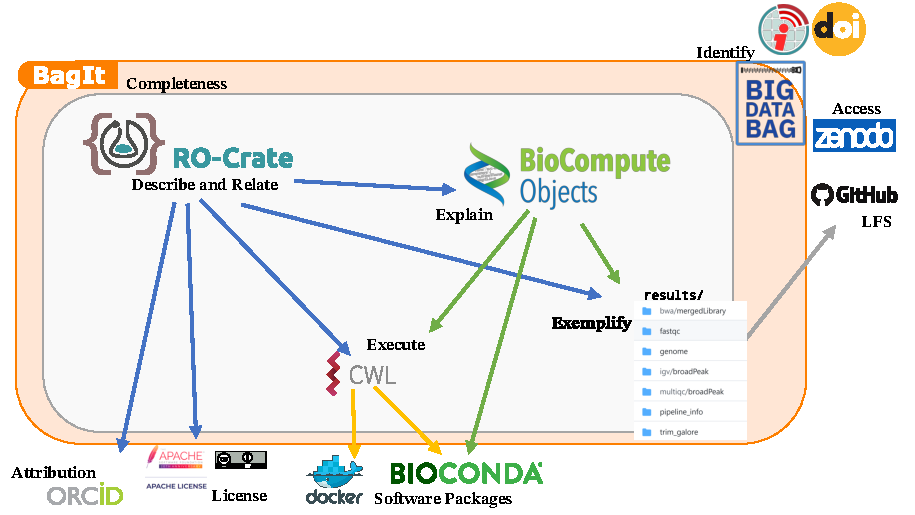
\includegraphics[width=\textwidth]{figures/ch05/ro-crate-bco-sep-of-concerns.pdf}
	\caption[Separation of Concerns in BCO RO-Crate]{\textbf{Separation of Concerns in BCO RO-Crate}. BioCompute
  Object (IEEE2791) is a JSON file that structurally explains the purpose
  and implementation of a computational workflow, for instance
  implemented in Common Workflow Language (CWL), that installs the
  workflow's software dependencies as Docker containers or BioConda
  packages. An example execution of the workflow shows the different
  kinds of result outputs, which may be external, using GitHub LFS \cite {ch5-85} to support larger data. RO-Crate gathers all these local
  and external resources, relating them and giving individual
  descriptions, for instance permanent DOI identifiers for reused
  datasets accessed from Zenodo, but also adding external identifiers to
  attribute authors using ORCID or to identify which licences apply to
  individual resources. The RO-Crate and its local files are captured in
  a BagIt whose checksum ensures completeness, combined with Big Data Bag
  \cite{Chard 2016} features to ``complete'' the
  bag with large external files such as the workflow outputs.}
  \label{ch5:fig:sep_concerns}
\end{figure}


\hypertarget{culturalheritage}{%
\subsubsection{Digital Humanities: Cultural
Heritage}\label{ch5:culturalheritage}}

The Pacific And Regional Archive for Digital Sources in Endangered
Cultures (PARADISEC\footnote{\url{https://www.paradisec.org.au/}}) \cite{ch5-114}
maintains a repository of more than 500,000 files documenting
endangered languages across more than 16,000 items, collected and
digitised over many years by researchers interviewing and recording
native speakers across the region.

The Modern PARADISEC demonstrator\footnote{\url{https://mod.paradisec.org.au/}} has
been
proposed\footnote{\url{https://arkisto-platform.github.io/case-studies/paradisec/}}
as an update to the 18 year old infrastructure, to also help long-term
preservation of these artefacts in their digital form. The demonstrator
uses RO-Crate to describe the overall structure and to capture the
metadata of each item. The existing PARADISEC data collection has been
ported and captured as RO-Crates. A Web portal then exposes the
repository and its entries by indexing the RO-Crate metadata files,
presenting a domain-specific view of the items -- the RO-Crate is
``hidden'' and does not change the user interface.


The PARADISEC use case takes advantage of several RO-Crate features and
principles. Firstly, the transcribed metadata are now independent of the
PARADISEC platform and can be archived, preserved and processed in its
own right, using Schema.org as base vocabulary and extended with
PARADISEC-specific terms.

In this approach, RO-Crate is the holder of itemised metadata, stored in
regular files that are organised using
Oxford Common File
Layout\footnote{\url{https://ocfl.io/1.0/spec/}} (OCFL)
\cite{ch5-96}, which ensures file integrity
and versioning on a regular shared file system. This lightweight
infrastructure also gives flexibility for future developments and
maintenance. For example a consumer can use Linked Data software such as
a graph database and query the whole corpora using SPARQL triple
patterns across multiple RO-Crates. For long term digital preservation,
beyond the lifetime of PARADISEC portals, a ``last resort'' fallback is
storing the generic RO-Crate HTML preview
\cite{ch5-95}. Such
human-readable rendering of RO-Crates can be hosted as static files by
any Web server, in line with the approach taken by the Endings
Project.\footnote{The Endings Project \url{https://endings.uvic.ca/} 
  is a five-year project funded by the Social Sciences and Humanities
  Research Council (SSHRC) that is creating tools, principles, policies
  and recommendations for digital scholarship practitioners to create
  accessible, stable, long-lasting resources in the humanities.}

\subsubsection{Machine-actionable Data Management Plans}\label{ch5:dmp}

Machine-actionable Data Management Plans (maDMPs) have been proposed as
an improvement to automate FAIR data management tasks in research
\cite{ch5-88}; maDMPs
use PIDs and controlled vocabularies to describe what happens to data
over the research life cycle
\cite{Cardoso 2020a}. The
Research Data Alliance's \emph{DMP Common Standard} for maDMPs
\cite{ch5-121} is one such
formalisation for expressing maDMPs, which can be expressed as Linked
Data using the DMP Common Standard Ontology
\cite{Cardoso 2020b}, a
specialisation of the W3C Data Catalog Vocabulary (DCAT)
\cite{DCAT2 2020}.
RDA maDMPs are usually expressed using regular JSON, conforming to the
DMP JSON Schema.

A mapping has been produced between Research Object Crates and
Machine-actionable Data Management Plans
\cite{Miksa 2020}, implemented by
the RO-Crate RDA maDMP Mapper
\cite{Arfaoui 2020}. A similar
mapping has been implemented by \emph{RO-Crate\_2\_ma-DMP}
\cite{Brenner 2020}. In both cases,
a maDMP can be converted to a RO-Crate, or vice versa. In
\cite{Miksa 2020} this
functionality caters for two use cases:

\begin{enumerate}
\item
  Start a skeleton data management plan based on an existing RO-Crate
  dataset, e.g.~an RO-Crate from WorkflowHub.
\item
  Instantiate an RO-Crate based on a data management plan.
\end{enumerate}

An important nuance here is that data management plans are (ideally)
written in \emph{advance} of data production, while RO-Crates are
typically created to describe data \emph{after} it has been generated.
What is significant to note in this approach is the importance of
\textbf{templating} in order to make both tasks automatable and
achievable, and how RO-Crate can fit into earlier stages of the research
life cycle.

\subsubsection{Institutional data repositories -- Harvard Data Commons}
\label{ch5:institutionalrepos}

The concept of a \textbf{Data Commons} for research collaboration was
originally defined as \emph{``cyber-infrastructure that co-locates data,
storage, and computing infrastructure with commonly used tools for
analysing and sharing data to create an interoperable resource for the
research community''}
\cite{ch5-59}. More recently,
Data Commons has been established to mean integration of active
data-intensive research with data management and archival best
practices, along with a supporting computational infrastructure.
Furthermore, the Commons features tools and services, such as
computation clusters and storage for scalability, data repositories for
disseminating and preserving regular, but also large or sensitive
datasets, and other research assets. Multiple initiatives were
undertaken to create Data Commons on national, research, and
institutional levels. For example, the Australian Research Data Commons
(ARDC)\footnote{\url{https://ardc.edu.au/}} 
\cite{Barker 2019} is a national
initiative that enables local researchers and industries to access
computing infrastructure, training, and curated datasets for
data-intensive research. NCI's Genomic
Data Commons\footnote{\url{https://gdc.cancer.gov/}} (GDC)
\cite{ch5-65} provides
the cancer research community with access to a vast volume of genomic
and clinical data. Initiatives such as
Research Data Alliance (RDA) Global Open Research Commons\footnote{\url{https://www.rd-alliance.org/groups/global-open-research-commons-ig}}
propose standards for
the implementation of Data Commons to prevent them becoming ``data
silos'' and thus, enable interoperability from one Data Commons to
another.

\textbf{Harvard Data Commons}
\cite{Crosas 2020} aims to address the
challenges of data access and cross-disciplinary research within a
research institution. It brings together multiple institutional schools,
libraries, computing centres and the
Harvard
Dataverse\footnote{\url{https://dataverse.harvard.edu/}} data repository.
Dataverse\footnote{\url{https://dataverse.org/}}
\cite{Crosas 2011} is a free
and open-source software platform to archive, share and cite research
data. The Harvard Dataverse repository is the largest of 70 Dataverse
installations worldwide, containing over 120K datasets with about 1.3M
data files (as of 2021-11-16). Working toward the goal of facilitating
collaboration and data discoverability and management within the
university, Harvard Data Commons has the following primary objectives:

\begin{enumerate}
\item
  the integration of Harvard Research Computing with Harvard Dataverse
  by leveraging Globus endpoints
  \cite{Chard 2014}; this will allow
  an automatic transfer of large datasets to the repository. In some
  cases, only the metadata will be transferred while the data stays
  stored in remote storage;
\item
  support for advanced research workflows and providing packaging
  options for assets such as code and workflows in the Harvard Dataverse
  repository to enable reproducibility and reuse, and
\item
  interation of repositories supported by Harvard, which include
  DASH\footnote{\url{https://dash.harvard.edu/}}, the open access institutional
  repository, the Digital Repository Services (DRS) for preserving
  digital asset collections, and the Harvard Dataverse.
\end{enumerate}

Particularly relevant to this article is the second objective of the
Harvard Data Commons, which aims to support the deposit of research
artefacts to Harvard Dataverse with sufficient information in the
metadata to allow their future reuse (Figure \vref{ch5:fig:hdc}). To support the incorporation of data, code, and other artefacts
from various institutional infrastructures, Harvard Data Commons is
currently working on RO-Crate adaptation. The RO-Crate metadata provides
the necessary structure to make all research artefacts FAIR. The
Dataverse software already has
extensive
support\footnote{\url{https://guides.dataverse.org/en/latest/user/appendix.html}} for metadata, including the Data Documentation Initiative
(DDI), Dublin Core, DataCite, and Schema.org. Incorporating RO-Crate,
which has the flexibility to describe a wide range of research
resources, will facilitate their seamless transition from one
infrastructure to the other within the Harvard Data Commons.

Even though the Harvard Data Commons is specific to Harvard University,
the overall vision and the three objectives can be abstracted and
applied to other universities or research organisations. The Commons
will be designed and implemented using standards and commonly-used
approaches to make it interoperable and reusable by others.

\begin{figure}%[t!]
  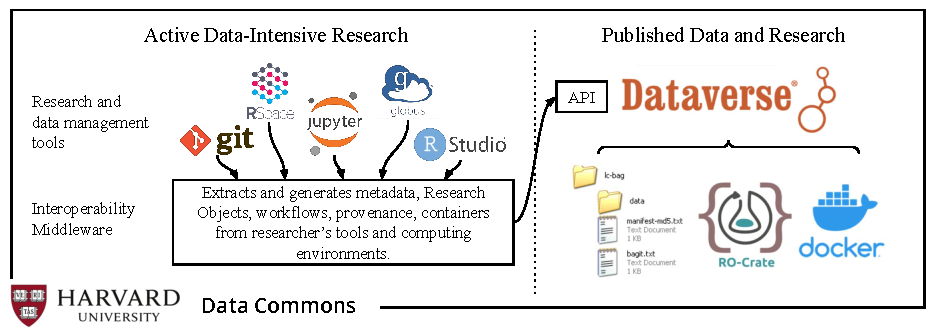
\includegraphics[width=1.1\textwidth]{figures/ch05/data-commons-ro-crate-figure-5.pdf}
	\caption[Harvard Data Commons]{\textbf{One aspect of Harvard Data Commons}. Automatic
  encapsulation and deposit of artefacts from data management tools used
  during active research at the Harvard Dataverse repository.}
  \label{ch5:fig:hdc}
\end{figure}

\subsection{Related Work}\label{ch5:relatedwork}

With the increasing digitisation of research processes, there has been a
significant call for the wider adoption of interoperable sharing of data
and its associated metadata. We refer to
\cite{ch5-72} for a
comprehensive overview and recommendations, in particular for data;
notably that review highlights the wide variety of metadata and
documentation that the literature prescribes for enabling data reuse.
Likewise, we suggest
\cite{Leipzig 2021} that
covers the importance of metadata standards in reproducible
computational research.

Here we focus on approaches for bundling research artefacts along with
their metadata. This notion of publishing compound objects for scholarly
communication has a long history behind it
\cite{Claerbout 1992,ch5-117},
but recent approaches have followed three main strands: (i) publishing to
centralised repositories; (ii) packaging approaches similar to RO-Crate;
and (iii) bundling the computational workflow around a scientific
experiment.

\subsubsection{Bundling and Packaging Digital Research
Artefacts}\label{ch5:bundling-and-packaging-digital-research-artefacts}

Early work making the case for publishing compound scholarly
communication units
\cite{ch5-117}
led to the development of the
Object Re-Use and Exchange
model\footnote{\url{http://www.openarchives.org/ore/1.0/primer}} (OAI-ORE), providing a structured \textbf{resource map}
of the digital artefacts that together support a scholarly output.

The challenge of describing computational workflows was one of the main
motivations for the early proposal of \emph{Research Objects} (RO)
\cite{Bechhofer 2013}
as first-class citizens for sharing and publishing. The RO approach
involves bundling datasets, workflows, scripts and results along with
traditional dissemination materials like journal articles and
presentations, forming a single package. Crucially, these resources are
not just gathered, but also individually typed, described and related to
each other using semantic vocabularies. As pointed out in
\cite{Bechhofer 2013} an
open-ended \emph{Linked Data} approach is not sufficient for scholarly
communication: a common data model is also needed in addition to common
and best practices for managing and annotating lifecycle, ownership,
versioning and attributions.

Considering the FAIR principles
\cite{Wilkinson 2016}, we can say with
hindsight that the initial RO approaches strongly targeted
\emph{Interoperability}, with a particular focus on the reproducibility
of \emph{in-silico experiments} involving computational workflows and
the reuse of existing RDF vocabularies.

The first implementation of Research Objects for sharing workflows in
myExperiment \cite{ch5-57} was
based on RDF ontologies
\cite{ch5-93}, building on
Dublin Core, FOAF, SIOC, Creative Commons and OAI-ORE to form
myExperiment ontologies for describing social networking, attribution
and credit, annotations, aggregation packs, experiments, view
statistics, contributions, and workflow components
\cite{ch5-92}.

This initially workflow-centric approach was further formalised as the
Wf4Ever Research Object Model
\cite{Belhajjame 2015}, which is
a general-purpose research artefact description framework. This model is
based on existing ontologies (FOAF, Dublin Core Terms, OAI-ORE and
AO/OAC precursors to the W3C Web Annotation Model
\cite{Ciccarese 2017})
and adds specializations for workflow models and executions using W3C
PROV-O \cite{w3-prov-o}.
The Research Object statements are saved in a \emph{manifest} (the
OAI-ORE \emph{resource map}), with additional annotation resources
containing user-provided details such as title and description.

We now claim that one barrier for wider adoption of the Wf4Eer Research
Object model for general packaging digital research artefacts was
exactly this re-use of multiple existing vocabularies (FAIR principle
I2: \emph{Metadata use vocabularies that follow FAIR principles}), which
in itself is recognized as a challenge
\cite{ch5-67}. Adapters
of the Wf4Ever RO model would have to navigate documentation of multiple
overlapping ontologies, in addition to facing the usual Semantic Web
development choices for RDF serialization formats, identifier minting
and publishing resources on the Web.

Several developments for Research Objects improved on this situation,
such as ROHub used by Earth Sciences
\cite{ch5-48}, which provides a
user-interface for making Research Objects, along with Research Object
Bundle \cite{ch5-111} (RO
Bundle), which is a ZIP-archive embedding data files and a JSON-LD
serialization of the manifest with mappings for a limited set of terms.
RO Bundle was also used for storing detailed workflow run provenance
(TavernaPROV
\cite{ch5-110}).

RO-Bundle evolved to Research Object
BagIt archives\footnote{\url{https://w3id.org/ro/bagit}}, a variant of RO Bundle as a BagIt archive
\cite{ch5-74}, used by Big Data Bags
\cite{Chard 2016},
CWLProv \cite{Khan 2019} and
WholeTale \cite{ch5-76,Chard 2019}.

\subsubsection{FAIR Digital Objects}\label{ch5:fair-digital-objects}

FAIR Digital Objects (FDO)
\cite{De Smedt 2020} have been
proposed as a conceptual framework for making digital resources
available in a Digital Objects (DO) architecture which encourages active
use of the objects and their metadata. In particular, an FDO has five
parts: (i) The FDO \emph{content}, bit sequences stored in an accessible
repository; (ii) a \emph{Persistent Identifier} (PID) such as a DOI that
identifies the FDO and can resolve these same parts; (iii) Associated
rich \emph{metadata}, as separate FDOs; (iv) Type definitions, also
separate FDOs; (v) Associated \emph{operations} for the given types. A
Digital Object typed as a Collection aggregates other DOs by reference.

The Digital Object Interface Protocol \cite{DONA 2018}
can be considered an ``abstract protocol'' of requirements, DOs could be
implemented in multiple ways. One suggested implementation is the 
FAIR Digital Object
Framework,\footnote{\url{https://fairdigitalobjectframework.org/}} based on HTTP and the Linked Data Principles. While there is
agreement on using PIDs based on DOIs, consensus on how to represent
common metadata, core types and collections as FDOs has not yet been
reached. We argue that RO-Crate can play an important role for FDOs:

\begin{enumerate}
\item
  By providing a predictable and extensible serialisation of structured
  metadata.
\item
  By formalising how to aggregate digital objects as collections (and
  adding their context).
\item
  By providing a natural Metadata FDO in the form of the RO-Crate
  Metadata File.
\item
  By being based on Linked Data and Schema.org vocabulary, meaning that
  PIDs already exist for common types and properties.
\end{enumerate}

At the same time, it is clear that the goal of FDO is broader than that
of RO-Crate; namely, FDOs are active objects with distributed
operations, and add further constraints such as PIDs for every element.
These features improve FAIR features of digital objects and are also
useful for RO-Crate, but they also severely restrict the infrastructure
that needs to be implemented and maintained in order for FDOs to remain
accessible. RO-Crate, on the other hand, is more flexible: it can
minimally be used within any file system structure, or ideally exposed
through a range of Web-based scenarios. A \emph{FAIR profile of
RO-Crate} (e.g.~enforcing PID usage) will fit well within a FAIR Digital
Object ecosystem.

\subsubsection{Packaging Workflows}\label{ch5:packaging-workflows}

The use of computational workflows, typically combining a chain of tools
in an analytical pipeline, has gained prominence in particular in the
life sciences. Workflows might be used primarily to improve
computational scalability, as well as to assist in making computed data
results FAIR \cite{Goble 2020}, for
instance by improving reproducibility
\cite{Cohen-Boulakia 2017}, but also
because programmatic data usage help propagate their metadata and
provenance \cite{ch5-69}. At the
same time, workflows raise additional FAIR challenges, since they can be
considered important research artefacts themselves. This viewpoint poses
the problem of capturing and explaining the computational methods of a
pipeline in sufficient machine-readable detail
\cite{Lamprecht 2019}.

Even when researchers follow current best practices for workflow
reproducibility
\cite{Gruning 2018b,Cohen-Boulakia 2017}, the
communication of computational outcomes through traditional academic
publishing routes effectively adds barriers as authors are forced to
rely on a textual manuscript representations. This hinder
reproducibility and FAIR use of the knowledge previously captured in the
workflow.

As a real-life example, let us look at a metagenomics article
\cite{Almeida 2019} that describes
a computational pipeline. Here the authors have gone to extraordinary
efforts to document the individual tools that have been reused,
including their citations, versions, settings, parameters and
combinations. The \emph{Methods} section is two pages in tight
double-columns with twenty four additional references, supported by the
availability of data on an FTP server (60 GB)
\cite{EMBL-EBI 2019}
and of open source code in GitHub
Finn-Lab/MGS-gut\footnote{\url{https://github.com/Finn-Lab/MGS-gut}}
\cite{EMBL-EBI 2020}, including the
pipeline as shell scripts and associated analysis scripts in R and
Python.

This attention to reporting detail for computational workflows is
unfortunately not yet the norm, and although bioinformatics journals
have strong \emph{data availability} requirements, they frequently do
not require authors to include or cite \emph{software, scripts and
pipelines} used for analysing and producing results \cite{ch5-108}.
Indeed, in the absence of a specific requirement and an editorial policy
to back it up -- such as eliminating the reference limit -- authors are
effectively discouraged from properly and comprehensively citing
software \cite{ch5-53}.

However detailed this additional information might be, another
researcher who wants to reuse a particular computational method may
first want to assess if the described tool or workflow is Re-runnable
(executable at all), Repeatable (same results for original inputs on
same platform), Reproducible (same results for original inputs with
different platform or newer tools) and ultimately Reusable (similar
results for different input data), Repurposable (reusing parts of the
method for making a new method) or Replicable (rewriting the workflow
following the method description)
\cite{Benureau 2017,ch5-54}.

Following the textual description alone, researchers would be forced to
jump straight to evaluate ``Replicable'' by rewriting the pipeline from
scratch. This can be expensive and error-prone. They would firstly need
to install all the software dependencies and download reference
datasets. This can be a daunting task, which may have to be repeated
multiple times as workflows typically are developed at small scale on
desktop computers, scaled up to local clusters, and potentially put into
production using cloud instances, each of which will have different
requirements for software installations.

In recent years the situation has been greatly improved by software
packaging and container technologies like Docker and Conda, these
technologies have been increasingly adopted in life sciences
\cite{ch6-4} thanks to
collaborative efforts such as BioConda
\cite{Gruning 2018a} and
BioContainers
\cite{da Veiga Leprevost 2017}, and
support by Linux distributions (e.g.~Debian Med
\cite{ch5-89}). As of
November 2021, more than 9,000 software packages are available in
BioConda alone,\footnote{\url{https://anaconda.org/bioconda/}} and 10,000 containers
in BioContainers.\footnote{\url{https://biocontainers.pro/\#/registry}}

Docker and Conda have been integrated into workflow systems such as
Snakemake
\cite{Koster 2012}, Galaxy
\cite{Afgan 2018} and Nextflow
\cite{Di Tommaso 2017}, meaning
a downloaded workflow definition can now be executed on a ``blank''
machine (except for the workflow engine) with the underlying analytical
tools installed on demand. Even with using containers there is a
reproducibility challenge, for instance Docker Hub's retention policy
will expire container images after six
months,\footnote{\url{https://www.docker.com/blog/docker-hub-image-retention-policy-delayed-and-subscription-updates/}}
or a lack of recording versions of transitive dependencies of Conda
packages could cause incompatibilities if the packages are subsequently updated.

These container and package systems only capture small amounts of
metadata\footnote{Docker and Conda can use \emph{build recipes}, a set
  of commands that construct the container image through downloading and
  installing its requirements. However these recipes are effectively
  another piece of software code, which may itself decay and become
  difficult to rerun.}. In particular, they do not capture any of the
semantic relationships between their content. Understanding these
relationships is made harder by the opaque wrapping of arbitrary tools
with unclear functionality, licenses and attributions.

From this we see that computational workflows are themselves complex
digital objects that need to be recorded not just as files, but in the
context of their execution environment, dependencies and analytical
purpose in research -- as well as other metadata (e.g.~version, license,
attribution and identifiers).

It is important to note that having all these computational details in
order to represent them in an RO-Crate is an ideal scenario -- in
practice there will always be gaps of knowledge, and exposing all
provenance details automatically would require improvements to the data
sources, workflow, workflow engine and its dependencies. RO-Crate can be
seen as a flexible annotation mechanism for augmenting automatic
workflow provenance. Additional metadata can be added manually, e.g.~for
sensitive clinical data that cannot be publicly exposed\footnote{FAIR
  principle A2: \emph{Metadata are accessible, even when the data are no
  longer available.}
  \cite{Wilkinson 2016}}, or to cite
software that lack persistent identifiers. This inline \emph{FAIRifying}
allows researchers to achieve ``just enough FAIR'' to explain their
computational experiments.

\hypertarget{conclusion}{%
\subsection{Conclusion}\label{ch5:conclusion}}

RO-Crate has been established as an approach to packaging digital
research artefacts with structured metadata. This approach assists
developers and researchers to produce and consume FAIR archives of their
research.

RO-Crate is formed by a set of best practice recommendations, developed
by an open and broad community. These guidelines show how to use ``just
enough'' standards in a consistent way. The use of structured metadata
with a rich base vocabulary can cover general-purpose contextual
relations, with a Linked Data foundation that ensures extensibility to
domain- and application-specific uses. We can therefore consider an
RO-Crate not just as a structured data archive, but as a multimodal
scholarly knowledge graph that can help ``FAIRify'' and combine metadata
of existing resources.

The adoption of simple Web technologies in the RO-Crate specification
has helped a rapid development of a wide variety of supporting open
source tools and libraries. RO-Crate fits into the larger landscape of
open scholarly communication and FAIR Digital Object infrastructure, and
can be integrated into data repository platforms. RO-Crate can be
applied as a data/metadata exchange mechanism, assist in long-term
archival preservation of metadata and data, or simply used at a small
scale by individual researchers. Thanks to its strong community support,
new and improved profiles and tools are being continuously added to the
RO-Crate landscape, making it easier for adopters to find examples and
support for their own use case.

\subsubsection{Strictness vs
flexibility}\label{ch5:strictness-vs-flexibility}

There is always a tradeoff between flexibility and strictness \cite{ch5-116}
when deciding on semantics of metadata models. Strict requirements make
it easier for users and code to consume and populate a model, by
reducing choices and having mandated ``slots'' to fill in. But such
rigidity can also restrict richness and applicability of the model, as
it in turn enforce the initial assumptions about what can be described.

RO-Crate attempts to strike a balance between these tensions, and
provides a common metadata framework that encourages extensions.
However, just like the RO-Crate specification can be thought of as a
\emph{core profile} of Schema.org in JSON-LD, we cannot stress the
importance of also establishing domain-specific RO-Crate profiles and
conventions, as explored in Sections~\vref{ch5:profiles} and \vref
{ch5:inuse}. Specialization comes
hand-in-hand with the principle of \emph{graceful degradation}; RO-Crate
applications and users are free to choose the semantic detail level they
participate at, as long as they follow the common syntactic
requirements.

\subsection{Future Work}\label{ch5:futurework}

The direction of future RO-Crate work is determined by the community
around it as a collaborative effort. We currently plan on further
outreach, building training material (including a comprehensive
entry-level tutorial) and maturing the reference implementation
libraries. We will also collect and build examples of RO-Crate
\emph{consumption}, e.g.~Jupyter Notebooks that query multiple crates
using knowledge graphs. In addition, we are exploring ways to support
some entity types requested by users, e.g.~detailed workflow runs or
container provenance, which do not have a good match in Schema.org. Such
support could be added, for instance, by integrating other vocabularies
or by having separated (but linked) metadata files.

Furthermore, we want to better understand how the community uses
RO-Crate in practice and how it contrasts with other related efforts;
this will help us to improve our specification and tools. By discovering
commonalities in emerging usage (e.g.~additional Schema.org types), the
community helps to reduce divergence that could otherwise occur with
proliferation of further RO-Crate profiles. We plan to gather feedback
via user studies, with the Linked Open Data community or as part of EOSC
Bring-your-own-Data training events.

We operate in an open community where future and potential users of
RO-Crate are actively welcomed to participate and contribute feedback
and requirements. In addition, we are targeting a wider audience through
extensive
outreach
activities\footnote{\url{https://www.researchobject.org/ro-crate/outreach.html}} and by initiating new connections. Recent contacts include
American Geophysical Union (AGU) on Data Citation Reliquary
\cite{Agarwal 2021}, National
Institute of Standards and Technology (NIST) on material science, and
InvenioRDM\footnote{\url{https://inveniosoftware.org/products/rdm/}} used by the
Zenodo data repository. New Horizon Europe projects adapting RO-Crate
include BY-COVID,\footnote{\url{https://by-covid.org/}} which aims to improve FAIR
access to data on COVID-19 and other infectious diseases.

The main addition in the upcoming 1.2 release of the RO-Crate
specifications will be the formalization of
profiles\footnote{\url{https://www.researchobject.org/ro-crate/1.2-DRAFT/profiles}}
for different categories of crates. Additional entity types have been
requested by users, e.g. workflow runs, business workflows, containers
and software packages, tabular data structures; these are not always
matched well with existing Schema.org types, but may benefit from other
vocabularies or even separate metadata files, e.g. from Frictionless
Data.\footnote{\url{https://frictionlessdata.io/}} We will be further aligning
and collaborating with related research artefact description efforts
like CodeMeta\footnote{\url{https://codemeta.github.io/}} for software metadata,
Science-on-Schema.org\footnote{\url{https://science-on-schema.org/}}
\cite{ch5-66} for datasets, FAIR Digital
Objects\footnote{\url{https://fairdo.org/}} \cite{De Smedt 2020} and
activities in EOSC task forces\footnote{\url{https://www.eosc.eu/task-force-faq}}
including the EOSC Interoperability Framework \cite{eosc-interop-framework}.

\section{Creating lightweight FAIR Digital Objects with RO-Crate}
\label{ch4:lightweight-fdo}

RO-Crate \cite{Soiland-Reyes 2022a} (section \ref{ch5:packaging-research-artefacts-with-ro-crate}) 
is a lightweight method to package research outputs along with
their metadata, based on Linked Data principles
\cite{Bizer 2009} and
W3C standards. RO-Crate provides a flexible mechanism for researchers
archiving and publishing rich data packages (or any other research
outcome) by capturing their dependencies and context.

However, additional measures should be taken to ensure that a crate is
also following the FAIR principles
\cite{Wilkinson 2016},
including consistent use of persistent identifiers, provenance,
community standards, clear machine/human-readable licensing for metadata
and data, and Web publication of RO-Crates.


The 
\acrfull{FDO}
%FAIR Digital Object (FDO) 
approach
\cite{De Smedt 2020}
gives a set of recommendations that aims to improve findability,
accessibility, interoperability and reproducibility for any digital
object, allowing implementation through different protocols or
standards.

Here we present how we have followed the FDO recommendations and turned
research outcomes into FDOs by publishing RO-Crates on the Web using
HTTP, following best practices for Linked Data. We highlight challenges
and advantages of the FDO approach, and reflect on what is required for
an FDO profile to achieve \acrshort{FAIR} RO-Crates.

The implementation allows for a broad range of use cases, across
scientific domains. A minimal RO-Crate may be represented as a
persistent URI resolving to a summary website describing the outputs in
a scientific investigation
(e.g.~\url{https://w3id.org/dgarijo/ro/sepln2022} with links to the used
datasets along with software).

One of the advantages of RO-Crates is flexibility, particularly
regarding the metadata accompanying the actual research outcome.
RO-Crate extends \cite{schema.org}, a popular
vocabulary for describing resources on the Web
\cite{Guha 2016}. A generic
RO-Crate is not required to be typed beyond \texttt{Dataset}\footnote{
  Resources described by an RO-Crate are also typed, e.g. \texttt{Person}, \texttt{Organization}, \texttt{ScholarlyArticle}, \texttt{ImageObject}. \\
  \url{https://www.researchobject.org/ro-crate/1.1/contextual-entities.html}
}
In practice, RO-Crates declare conformance to particular
\footurl{https://www.researchobject.org/ro-crate/profiles.html}{profiles},
allowing processing based on the specific needs and assumptions of a
community or usage scenario. This, effectively, makes RO-Crates typed
and thus machine-actionable. RO-Crate profiles serve as metadata
templates, making it easier for communities to agree and build upon
their own metadata needs.

RO-Crates have been combined with \emph{machine-actionable Data
Management Plans} (maDMPs) to automate and facilitate management of
research data \cite{Miksa 2020}. This mapping allows RO-Crates to be generated out of maDMPs
and vice versa. The ELIXIR Software Management Plans
\cite{Alves 2021} is
planning to move their questionnaire to a machine-actionable format with
RO-Crate. ELIXIR \footurl{https://biohackathon-europe.org/}{Biohackathon}
2022 will\footnote{See report \cite{Eguinoa 2023}}
\footurl{https://github.com/elixir-europe/biohackathon-projects-2022/tree/main/10}{explore}
integration of RO-Crate and the \footurl{https://ds-wizard.org/}{Data
Stewardship Wizard} 
\cite{Pergl 2019} with Galaxy, which can automate FDO creation that also follows
data management plans.

A tailored RO-Crate profile has been defined to represent Electronic Lab
Notebooks (ELN) protocols bundled together with metadata and related
datasets. \cite{Schröder 2022} uses RO-Crates to encode provenance information at different
levels, including researchers, manufacturers, biological and chemical
resources, activities, measurements, and resulting research data. The
use of RO-Crates makes it easier to programmatically question-answer
information related to the protocols, for instance activities, resources
and equipment used to create data.

Another example is \footurl{https://workflowhub.eu/}{WorkflowHub}
\cite{Goble 2021} which
defines the
\footurl{https://w3id.org/workflowhub/workflow-ro-crate/1.0}{Workflow
RO-Crate} profile
\cite{Bacall 2022}, imposing additional constraints such as the presence of a main
workflow and a license. It also specifies which entity types and
properties must be used to provide such information, implicitly defining
a set of operations (e.g., get the main workflow and its language) that
are valid on all complying crates. The workflow system Galaxy
\cite{Galaxy 2022} retrieves
such Workflow Crates using
\footurl{https://about.workflowhub.eu/developer/trs/}{GA4GH TRS API}.

The workflow profile has been further extended (with OOP-like
inheritance) in
\footurl{https://crs4.github.io/life_monitor/workflow_testing_ro_crate}{Workflow Testing}
RO-Crate, adding formal workflow testing components: this adds
operations such as getting remote test instances and test definitions,
used by the \footurl{https://www.lifemonitor.eu/}{LifeMonitor} service to
keep track of the health status of multiple published workflows.

While RO-Crates use Web technologies, they are also
\emph{self-contained}, moving data along with their metadata. This is a
powerful construct for interoperability across FAIR repositories, but
this raises some challenges with regards to mutability and persistence
of crates.

To illustrate how such challenges can be handled, we detail how the
WorkflowHub repository follows several FDO principles\footnote{
  See table \vref{ch10:fdo-guidelines}
}:

\begin{enumerate}

\item
  Workflow entries must be \emph{frozen} for editing and have complete
  kernel metadata (title, authors, license, description) {[}FDOF4{]}
  before they can be assigned a persistent identifier,
  e.g.~\url{https://doi.org/10.48546/workflowhub.workflow.255.1}
  {[}FDOF1{]}
\item
  Computational workflows can be composed of multiple files used as a
  whole, e.g.~CWL files in a GitHub repository. These are snapshotted as
  a single RO-Crate ZIP, indicating the main workflow. {[}FDOF11{]}
\item
  PID resolution can content-negotiate to Datacite's PID metadata
  {[}FDOF2{]} or use \footurl{https://signposting.org/FAIR/}{FAIR
  Signposting} to find an RO-Crate containing the workflow {[}FDOF3{]}
  and richer JSON-LD metadata resources {[}FDOF5,FDOF8{]}, see
  Figure \vref{fig:signposting}.
\item
  Metadata uses schema.org {[}FDOF7{]} following the community-developed
  Bioschemas
  \footurl{https://bioschemas.org/profiles/ComputationalWorkflow/1.0-RELEASE}{ComputationalWorkflow}
  profile {[}FDOF10{]}.
\item
  Workflows are discovered using
  the\footurl{https://about.workflowhub.eu/developer/trs/}{GA4GH TRS API}
  {[}FDOF5,FDOF6,FDOF11{]} and created/modified using
  \footurl{https://workflowhub.eu/api}{CRUD operations} {[}FDOF6{]}
\item
  The RO-Crate profile, effectively the FDO Type {[}FDOF7{]}, is
  declared as \url{https://w3id.org/workflowhub/workflow-ro-crate/1.0};
  the workflow language
  (e.g.~\url{https://w3id.org/workflowhub/workflow-ro-crate\#galaxy} is
  defined in metadata of the main workflow.
\end{enumerate}



%% Prepare for 4 evil footnotes
\begin{figure}
  \centering
  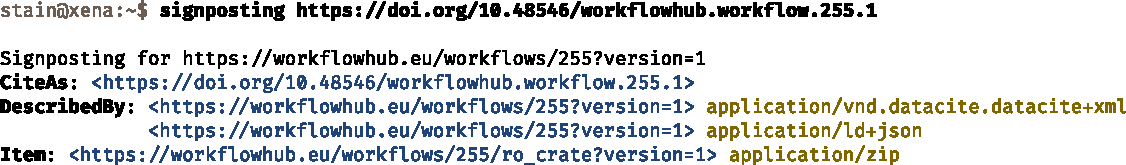
\includegraphics[width=\textwidth]{figures/ch04/signposting.pdf}
  \caption[FAIR Signposting]{~\textbf{FAIR Signposting}.
  FAIR Signposting on a workflow PID \cite{Bayarri 2022} 
  discovered from HTTP \texttt{Link:} headers using the
  Signposting tool\footnotemark{} shows
  machine-actionable navigation to content-negotiate for the metadata
  FDOs, as well as download bit sequence (FDOF3) as an RO-Crate ZIP.
  JSON-LD\footnotemark{} from
  workflowhub.eu follows the BioSchemas
  ComputationalWorkflow
  profile\footnotemark{}
  to give workflow details not included in DataCite's general 
  JSON-LD\footnotemark.
  }
  \label{fig:signposting}
\end{figure} 
% Evil goes here
\addtocounter{footnote}{-4}
\addtocounter{footnote}{1}\footnotetext{\url{https://pypi.org/project/signposting/}}
\addtocounter{footnote}{1}\footnotetext{\url{https://workflowhub.eu/workflows/255.jsonld}}
\addtocounter{footnote}{1}\footnotetext{\url{https://bioschemas.org/profiles/ComputationalWorkflow/1.0-RELEASE}}
\addtocounter{footnote}{1}\footnotetext{\url{https://data.crosscite.org/application/ld+json/10.48546/workflowhub.workflow.255.1}}
%%

Further work on RO-Crate profiles include to formalise links to the API
operations and repositories (FDOF5,FDOF7), to include PIDs of
profiles and types in the FAIR Signposting, and HTTP navigation to
individual resources within the RO-Crate.

RO-Crate has shown a broad adoption by communities across many
scientific disciplines, providing a lightweight, and therefore easy to
adopt, approach to generating FAIR Digital Objects (Figure \vref{ch9:fig:signposting}). It is rapidly
becoming an integral part of the interoperability fabric between the
different components as demonstrated here for WorkflowHub, contributing
to building the European Open Science Cloud.


\begin{figure}[htb]
  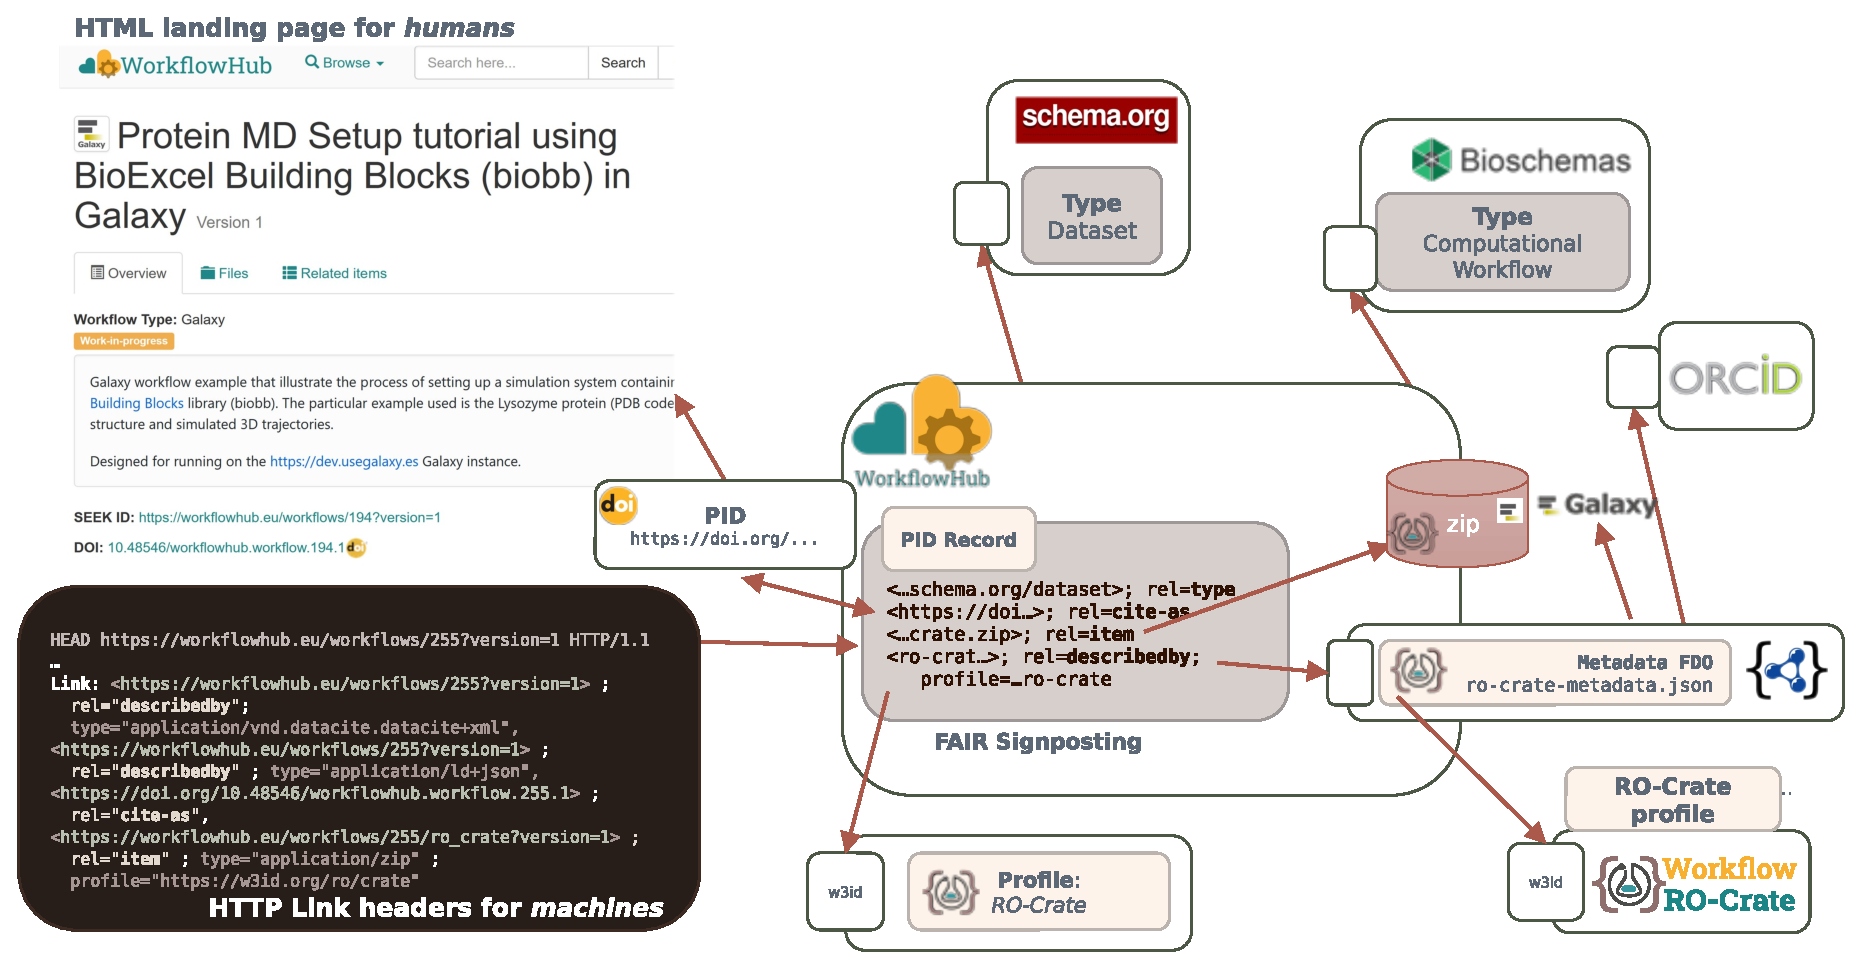
\includegraphics[width=\textwidth]{figures/ch09/signposting.pdf}
    \caption[WorkflowHub FDOs using Signposting and RO-Crate]{\textbf{WorkflowHub FDOs using Signposting and RO-Crate}. In this implementation of FDO (compare with figure \vref{ch3:fig:fdo}), WorkflowHub uses DOIs for persistent identifiers, which for human readers resolve to a landing page. Machine clients can extract the FAIR Signposting \texttt{Link} headers \cite{Van de Sompel 2022} to form the FDO PID Record. Link relation \texttt{cite-as} provides the PID \cite{Bayarri 2022} (in case the WorkflowHub page was discovered in other ways), and \texttt{describedby} links to the metadata FDO in JSON-LD format. Within the metadata file it indicates conformance to the Workflow RO-Crate profile (a Profile Crate FDO), while \texttt{item} links to the downloadable ZIP archive, which contains both the Galaxy workflow files and the RO-Crate metadata file. Alternative metadata in XML following the DataCite Metadata Schema is also linked to using \texttt{describedby}. Link relation \texttt{type} in the Signposting can provide the FDO type; this is not yet implemented by WorkflowHub -- it is currently unclear if this type should be a \emph{Dataset} (the download from this landing page is an RO-Crate) and/or \emph{ComputationalWorkflow} (the PID/page/crate identifies and describes a workflow).
    }
  \label{ch9:fig:signposting}
\end{figure}

\section{Formalizing RO-Crate in First Order Logic}
\label{ch5:formaldefinition}

Below is a formalization of the concept of RO-Crate as a set of relations using First Order Logic:

\subsection{Language}

Definition of language $\mathcal{L}_{rocrate}$:

\begin{eqnarray*}
    \mathcal{L}_{rocrate}   & = & \big\{ Property(p), Class(c),
                            Value(x), \mathbb{R}, \mathbb{S} \big\} \\
    \mathbb{D}              & = & \mathbb{IRI} \\
    \mathbb{IRI}            & \equiv & { \text{IRIs as defined in RFC3987 \cite{Duerst 2005} } } \\
    \mathbb{R}              & \equiv & { \text{real or integer numbers} } \\
    \mathbb{S}              & \equiv & { \text{literal strings} }
\end{eqnarray*}


The domain of discourse $\mathbb{D}$ is the set of $\mathbb{IRI}$ identifiers (notation $\texttt{<http://example.com/>}$)\footnote{
    For simplicity, blank nodes are not included in this formalisation, as RO-Crate
    recommends the use of IRI identifiers: \url{https://www.researchobject.org/ro-crate/1.1/appendix/jsonld.html\#describing-entities-in-json-ld}
}, with additional descriptions using numbers $\mathbb{R}$ (notation $13.37$) and literal strings $\mathbb{S}$ (notation $\text{“Hello”}$).

From this formalised language $\mathcal{L}_{rocrate}$ we can interpret an RO-Crate in any representation that can gather these descriptions, their properties, classes, and literal attributes.

\subsection{Minimal RO-Crate}

The definitions \vpageref[below]{ch5:minimalcrate} use $\mathcal{L}_{rocrate}$ for a minimal\footnote{
    The full list of types, relations and attribute properties from the RO-Crate specification are not included. Examples shown include $datePublished$, $CreativeWork$ and $name$.
} RO-Crate:


\small
\begin{eqnarray*}
\label{ch5:minimalcrate}
ROCrate(R)                                  & \models & Root(R) \land Mentions(R, R) \land hasPart(R, d) \land \\
                                            & & Mentions(R, d) \land DataEntity(d) \land \\
                                            & & Mentions(R, c) \land ContextualEntity(c) \\
\forall r \ Root(r)                         & \Rightarrow & Dataset(r) \land name(r, n) \land description(r, d) \land \\
                                            & &             datePublished(r, date) \land license(e, l) \\
\forall e \forall n \ name(e, n)            & \Rightarrow & Value(n) \\
\forall e \forall s \ description(e, s)     & \Rightarrow & Value(s) \\
\forall e \forall d \ datePublished(e, d)   & \Rightarrow & Value(d) \\
\forall e \forall l \ license(e, l)         & \Rightarrow & ContextualEntity(l) \\
DataEntity(e)                               & \equiv &      File(e) \oplus Dataset(e) \\
Entity(e)                                   & \equiv &      DataEntity(e) \lor ContextualEntity(e) \\
\forall e \ Entity(e)                       & \Rightarrow & type(e, c) \land Class(c) \\
\forall e \ ContextualEntity(e)             & \Rightarrow & name(e, n)  \\
Mentions(R, s)                              & \models &     Relation(s, p, e) \oplus Attribute(s,  p, l) \\
Relation(s, p, o)                           & \models &     Entity(s) \land Property(p) \land  Entity(o) \\
Attribute(s, p, v)                          & \models &     Entity(s) \land Property(p) \land Value(v) \\
Value(v)                                    & \equiv &      v \in \mathbb{R} \oplus v \in \mathbb{S}
\end{eqnarray*}
\normalsize

An $ROCrate(R)$ is defined as a self-described \emph{Root Data Entity}, which contains parts (\emph{data entities}), which are further described in \emph{contextual entities}.  These terms align with their use in the RO-Crate 1.1 terminology\footnote{
    \url{https://www.researchobject.org/ro-crate/1.1/terminology}}.

The $Root(r)$ is a type of $Dataset(r)$, and must as metadata have at least the attributes $name$, $description$ and $datePublished$, as well as a contextual entity that identify its $license$. These predicates correspond to the RO-Crate 1.1 minimal requirements for the root data entity\footnote{
    \url{https://www.researchobject.org/ro-crate/1.1/root-data-entity.html\#direct-properties-of-the-root-data-entity}
}.

The concept of an $Entity(e)$ is introduced as being either a $DataEntity(e)$, a $ContextualEntity(e)$, or both\footnote{
    \url{https://www.researchobject.org/ro-crate/1.1/contextual-entities.html\#contextual-vs-data-entities}
}. Any $Entity(e)$ must be typed with at least one $Class(c)$, and every $ContextualEntity(e)$ must also have a $name(e,n)$; this corresponds to expectations for any \emph{referenced contextual entity} (section \vref{ch5:contextualentities}). 

For simplicity in this formalization (and to assist production rules below) $R$ is a constant representing a single RO-Crate, typically written to independent RO-Crate Metadata files. $R$ is used by $Mentions(R, e)$ to indicate that $e$ is an Entity described by the RO-Crate and therefore its metadata (a set of $Relation$ and $Attribute$ predicates) form part of the RO-Crate serialization. $Relation(s, p, o)$ and $Attribute(s, p, x)$ are defined as a \emph{subject—predicate—object} triple pattern from an $Entity(s)$ using a $Property(p)$ to either another $Entity(o)$ or a $Value(x)$ value.

\subsection{Example of formalized RO-Crate}

The below is an example RO-Crate represented using the above formalisation, assuming a base IRI of \texttt{<http://example.com/ro/123/>}:

\allowdisplaybreaks
\small
\begin{eqnarray*}
&& ROCrate(\texttt{<http://example.com/ro/123/>}) \\
&& name(\texttt{<http://example.com/ro/123/>}, \\
&& \ \ \ \ \ \text{“Data files associated with the manuscript:Effects of …”}) \\
&& description(\texttt{<http://example.com/ro/123/}, \\
&& \ \ \ \ \ \text{“Palliative care planning for nursing home residents …”}) \\
&& license(\texttt{<http://example.com/ro/123/>}, \\
&& \ \ \ \ \ \texttt{<https://spdx.org/licenses/CC-BY-4.0>}) \\
&& datePublished(\texttt{<http://example.com/ro/123/>}, \text{“2017-02-23”}) \\
&& hasPart(\texttt{<http://example.com/ro/123/>}, \\
&& \ \ \ \ \ \texttt{<http://example.com/ro/123/file.txt>}) \\
&& hasPart(\texttt{<http://example.com/ro/123/>}, \\
&& \ \ \ \ \ \texttt{<http://example.com/ro/123/interviews/>}) \\
\\
&& ContextualEntity(\texttt{<https://spdx.org/licenses/CC-BY-4.0>}) \\
&& name(\texttt{<https://spdx.org/licenses/CC-BY-4.0>},  \\
&& \ \ \ \ \  \text{“Creative Commons Attribution 4.0”}) \\
\\
&& ContextualEntity(\texttt{<https://spdx.org/licenses/CC-BY-NC-4.0>}) \\
&& name(\texttt{<https://spdx.org/licenses/CC-BY-NC-4.0>},  \\
&& \ \ \ \ \  \text{“Creative Commons Attribution Non Commercial 4.0”}) \\
\\
&& File(\texttt{<http://example.com/ro/123/survey.csv>}) \\
&& name(\texttt{<http://example.com/ro/123/survey.csv>},
        \text{“Survey of care providers”}) \\
\\
&& Dataset(\texttt{<http://example.com/ro/123/interviews/>}) \\
&& name(\texttt{<http://example.com/ro/123/interviews/>},  \\
&& \ \ \ \ \  \text{“Audio recordings of care provider interviews”}) \\
&& license(\texttt{<http://example.com/ro/123/interviews/>}, \\
&& \ \ \ \ \ \texttt{<https://spdx.org/licenses/CC-BY-NC-4.0>})
\end{eqnarray*}
\normalsize

Notable from this triple-like formalization is that a RO-Crate $R$ is fully represented as a tree at depth 2 helped by the use of $\mathbb{IRI}$  nodes. For instance the aggregation from the root entity $hasPart(\texttt{…interviews/>})$ is at same level as the data entity’s property $license(\texttt{…CC-BY-NC-4.0>})$ and that contextual entity’s attribute $ name(\text{…Non Commercial 4.0”})$. As shown in section \vref{ch5:jsonld}, the RO-Crate Metadata File serialization is an equivalent shallow tree, although at depth 3 to cater for the JSON-LD preamble of \texttt{"@context"} and \texttt{"@graph"}.

In reality many additional attributes and contextual types from Schema.org types like \url{http://schema.org/affiliation} and \url{http://schema.org/Organization} would be used to further describe the RO-Crate and its entities, but as these are optional (\textit{SHOULD} requirements) they do not form part of this formalization.


\subsection{Mapping to RDF with Schema.org}

A formalized RO-Crate in $\mathcal{L}_{rocrate}$ can be mapped to different serializations.
Assume a simplified\footnote{
 This simplification and mapping does not cover the extensive list of literal datatypes built into RDF 1.1, only strings and decimal real numbers. Likewise, $LanguageTag$ is deliberately not utillised below.
} language $\mathcal{L}_{RDF}$
based on the RDF abstract syntax \cite{RDF 1.1 2014}:

\small
\begin{eqnarray*}
\mathcal{L}_{RDF}           & \equiv &      \big\{ Triple(s,p,o), IRI(i), BlankNode(b), Literal(s),
    \mathbb{IRI}, \mathbb{S}, \mathbb{R}    \big\} \\
\mathbb{D}_{RDF}            & \equiv &      \mathbb{S} \\
\forall i \ IRI(i)          & \Rightarrow & i \in \mathbb{IRI} \\
\forall s \forall p \forall o \
    Triple(s,p,o)           & \Rightarrow & \Big( IRI(s) \lor BlankNode(s) \Big) \land  \\
                            & &             IRI(p) \land  \\
                            & &             \Big(IRI(o) \lor BlankNode(o) \lor Literal(o) \Big) \\
Literal(v)                  & \models &     Value(v) \land Datatype(v,t) \land IRI(t) \\
\forall v \ Value(v)        & \Rightarrow & v \in \mathbb{S} \\
LanguageTag(v, l)           & \equiv &      Datatype\big(v, \\
    && \texttt{<http://www.w3.org/1999/02/22-rdf-syntax-ns\#langString>}\big)
\end{eqnarray*}
\normalsize

Below follows a mapping from $\mathcal{L}_{rocrate}$ to $\mathcal{L}_{RDF}$ using Schema.org as vocabulary:

\small
\begin{eqnarray*}
Property(p)         & \Rightarrow &     type(p, \texttt{<http://www.w3.org/2000/01/rdf-schema\#Property>})   \\
Class(c)            & \Rightarrow &     type(c, \texttt{<http://www.w3.org/2000/01/rdf-schema\#Class>})  \\
Dataset(d)          & \Rightarrow &     type(d, \texttt{<http://schema.org/Dataset>})   \\
File(f)             & \Rightarrow &     type(f, \texttt{<http://schema.org/MediaObject>})   \\
ContextualEntity(e) & \Rightarrow &     type(f, \texttt{<http://schema.org/Thing>})   \\
CreativeWork(e)     & \Rightarrow &     ContextualEntity(e) \\
                    & & \land type(e, \texttt{<http://schema.org/CreativeWork>})  \\
hasPart(e, t)       & \Rightarrow &     Relation(e, \texttt{<http://schema.org/hasPart>}, t)    \\
name(e, n)          & \Rightarrow &     Attribute(e, \texttt{<http://schema.org/name>}, n)  \\
description(e, s)   & \Rightarrow &     Attribute(e, \texttt{<http://schema.org/description>}, s)   \\
datePublished(e, d) & \Rightarrow &     Attribute(e, \texttt{<http://schema.org/datePublished>}, d) \\
license(e, l)       & \Rightarrow &     Relation(e, \texttt{<http://schema.org/license>}, l) \land CreativeWork(l) \\
type(e, t)          & \Rightarrow &     Relation(e, \texttt{<http://www.w3.org/1999/02/22-rdf-syntax-ns\#type>}, t) \\
                    & & \land Class(t)   \\
String(s)           & \equiv &          Value(s) \land  s \in \mathbb{S} \\
String(s)           & \Rightarrow &     Datatype(s, \texttt{<http://www.w3.org/2001/XMLSchema\#string>}) \\
Decimal(d)          & \equiv &          Value(d) \land  d \in \mathbb{R} \\
Decimal(d)          & \Rightarrow &     Datatype(d, \texttt{<http://www.w3.org/2001/XMLSchema\#decimal>}) \\
Relation(s,p,o)     & \Rightarrow &     Triple(s,p,o) \land IRI(s) \land IRI(o) \\
Attribute(s,p,o)    & \Rightarrow &     Triple(s,p,o) \land IRI(s) \land Literal(o) \\
\end{eqnarray*}
\normalsize

Note that in the JSON-LD serialization of RO-Crate, the expression of $Class$ and $Property$ is typically indirect: The JSON-LD \texttt{@context} maps to Schema.org IRIs, which, when resolved as Linked Data, embed their formal definition as RDFa. Extensions may however include such term definitions directly in the RO-Crate.

\subsection{RO-Crate 1.1 Metadata File Descriptor}

An important RO-Crate principle is that of being \textbf{self-described}. Therefore the serialisation of the RO-Crate into a file should also describe itself in a Metadata File Descriptor\footnote{
    \url{https://www.researchobject.org/ro-crate/1.1/root-data-entity.html\#ro-crate-metadata-file-descriptor}
}, indicating it is $about$ (describing) the RO-Crate root data entity, and that it $conformsTo$ a particular version of the RO-Crate specification:

\small
\begin{eqnarray*}
about(s,o)      & \Rightarrow & Relation(s, \texttt{<http://schema.org/about>}, o)   \\
conformsTo(s,o) & \Rightarrow & Relation(s, \texttt{<http://purl.org/dc/terms/conformsTo>}, o)   \\
MetadataFile(m) & \Rightarrow & CreativeWork(m) \land about(m,R) \land ROCrate(R) \land    \\
                &             & conformsTo(m, \texttt{<https://w3id.org/ro/crate/1.1>})
\end{eqnarray*}
\normalsize

Note that although the metadata file necessarily is an \emph{information resource} written to disk or served over the network (as JSON-LD), it is not considered to be a contained \emph{part} of the RO-Crate in the form of a \emph{data entity}, rather it is described only as a \emph{contextual entity}.

In the conceptual model, the \emph{RO-Crate Metadata File} can be seen as the top-level node that describes the \emph{RO-Crate Root}, however in the formal model (and the JSON-LD format) the metadata file descriptor is an additional contextual entity that is not affecting the depth-limit of the RO-Crate.

\subsection{Forward-chained Production Rules for JSON-LD}

Combining the above predicates and Schema.org mapping with rudimentary JSON templates, these forward-chaining production rules can output JSON-LD according to the RO-Crate 1.1 specification\footnote{
    \textbf{Limitations:} Contextual entities not related from the RO-Crate (e.g. using inverse relations to a data entity) would not be covered by the single direction $Mentions(R, s)$ production rule; see GitHub issue ResearchObject/ro-crate\#122 (\url{https://github.com/ResearchObject/ro-crate/issues/122}).\\
    The $datePublished(e, d)$ rule do not include syntax checks for the ISO 8601 datetime format. Compared with RO-Crate examples, this generated JSON-LD does not use a $@context$ as the IRIs are produced unshortened, a post-step could do JSON-LD Flattening with a versioned RO-Crate context. The \texttt{@type} expansion is included for clarity, even though this is also implied by the $type(e, t)$ expansion to $Relation(e, \texttt{xsd:type})$.
}:

\small
\begin{eqnarray*}
Mentions(R, s) \land Relation(s,p,o)
                        & \Rightarrow & Mentions(R, o) \\
IRI(i)                  & \Rightarrow & \texttt{"} i \texttt{"} \\
Decimal(d)              & \Rightarrow & d \\
String(s)               & \Rightarrow & \texttt{"} s \texttt{"} \\
\forall e \forall t
\ type(e, t)            & \Rightarrow & \texttt{\{"@id":}  e \texttt{,} \\
&&                               \ \  \texttt{"@type":} t \\
&&                              \texttt{\}} \\
\forall s \forall p \forall o
\ Relation(s,p,o)
                        & \Rightarrow &  \texttt{\{"@id":}  s \texttt{,} \\
&&                               \ \  p \texttt{: \{ "@id":} o \texttt{\}} \\
&&                              \texttt{\}} \\
\forall s \forall p \forall v
\ Attribute(s,p,v)    & \Rightarrow &  \texttt{\{"@id":} s \texttt{,} \\
&&                               \ \ p \texttt{:} v  \\
&&                               \texttt{\}} \\
\forall r  \forall c
    ROCrate(r)      & \Rightarrow &  \texttt{\{ "@graph": [} \\
&& \ \ \ \ Mentions(r, c)* \\
&& \ \ \ \texttt{]} \\
&& \texttt{\}} \\
R   & \equiv & \texttt{<./>}  \\
R   & \Rightarrow &  MetadataFile(\texttt{<ro-crate-metadata.json>}) \\
\end{eqnarray*}
\normalsize

This exposes the first order logic domain of discourse of IRIs, with rational numbers and strings as their corresponding JSON-LD representation. These production rules first grow the graph of $R$ by adding a transitive rule – anything described in $R$ which is related to $o$, means that $o$ is also mentioned by the $ROCrate(R)$. For simplicity this rule is one-way; in theory the graph can also contain free-standing contextual entities that have outgoing relations to data- and contextual entities, but these are proposed to be bound to the root data entity with Schema.org relation \footurl{http://schema.org/mentions}{mentions}.


\chapter{Computational Workflows}
\label{chapter:workflows}
In order to investigate \textbf{RQ3} (\vpageref*{rq3}), and considering an important part of the FAIR principles is \emph{Reuse} and \emph{provenance}, this chapter examines in closer details how FAIR Digital Objects and RO-Crate can be used with \textbf{Computational Workflows}. 

Section \vref{ch6:making-canonical-workflow-building-blocks-interoperable-across-workflow-languages} proposes that tools in computational workflows, when wrapped as interoperable building blocks, can be considered as FAIR Digital Objects, with a use case from biomolecular simulation.

Sections \vref{ch8:the-specimen-data-refinery} and \vref{ch7:incrementally-building-fair-digital-objects-with-specimen-data-refinery-workflows} explore how FDOs and Research Objects can be constructed incrementally using computational workflows, with a use case from specimen digitization in natural history collections.

Section \vref{ch54:wrroc} presents a profile of RO-Crate to capture workflow execution provenance, with incremental granularity levels and six workflow engine implementations. Use cases include machine learning-aided tumour detection and compatibility with PROV approaches. 

Supplementary materials that may assist readers of this chapter provide further details on FAIR Computational Workflows \cite{Goble 2020}, \footurl{https://s11.no/2021/phd/workflow-collaboratory/}{WorkflowHub} \cite{Goble 2021}, \footurl{https://s11.no/2022/phd/methods-included/}{Common Workflow Language} \cite{Crusoe 2022} and \footurl{https://s11.no/2022/phd/10-simple-rules-for-workflow-tools/}{making a software tool workflow ready} \cite{Brack 2022a}. 

On the aspects of workflow provenance, recommended reading in supplementary materials covers CWLProv \cite{Khan 2019}, \footurl{https://s11.no/2022/phd/galaxy-ro-crate/}{RO-Crate in Galaxy} \cite{De Geest 2022} and Common Provenance Model \cite{Wittner 2020,Wittner 2023a}.

\section{Making Canonical Workflow Building Blocks interoperable across
workflow
languages}
\label{ch6:making-canonical-workflow-building-blocks-interoperable-across-workflow-languages}

We introduce the concept of \emph{Canonical Workflow Building Blocks} (CWBB), a methodology of describing and wrapping computational tools, in order for them to be utilised in a reproducible manner from multiple workflow languages and execution platforms.
The concept is implemented and demonstrated with the BioExcel Building Blocks library (BioBB), a collection of tool wrappers in the field of computational biomolecular simulation.
Interoperability across different workflow languages is showcased through a protein Molecular Dynamics setup transversal workflow, built using this library and run with 5 different 
\acrfullpl{WfM}
%Workflow Manager Systems (WfMS).
We argue such practice is a necessary requirement for FAIR Computational Workflows and an element of Canonical Workflow Frameworks for Research (CWFR) in order to improve widespread adoption and reuse of computational methods across workflow language barriers.

\subsection{Introduction}\label{ch6:introduction}

The need for \emph{reproducibility} of research software usage is well established \cite{Stodden 2016,Leipzig 2021,Katz 2021a}, and adaptation of \emph{workflow management systems} (\textbf{WfMS}) together with \emph{software packaging and containers} \cite{Möller 2017} have been proposed as key ingredients for making research software usage \acrshort{FAIR} and reproducible \cite{Cohen-Boulakia 2017,Grüning 2018b,Lamprecht 2019}.
Recently it is also argued that computational workflows should also be treated as \acrfullpl{FDO} \cite{De Smedt 2020} in their own right, with identifier, metadata \cite{Leipzig 2021} and interoperability requirements \cite{Goble 2020}.

\footurl{https://bioexcel.eu/}{BioExcel}, a European Centre of Excellence for Computational Biomolecular Research, has a particular focus on the research domains molecular dynamics simulations and bioinformatics with use of \emph{High Performance Computing} (\textbf{HPC}) to approach Exascale performance, while also improving usability.
The \emph{BioExcel Building Blocks} (\textbf{BioBB}) \cite{Andrio 2019} have been created as portable wrappers of open-source computational tools identified as useful for BioExcel workflows, forming several \emph{families} of documented and interoperable operations that can be called from multiple workflow systems.
This interoperability is shown with the BioBB demonstrator workflows, along with multiple tutorials and notebooks.

We propose that these building blocks and their families can themselves be considered \emph{composite Digital Objects}: collections of software packages and their source code, guides and tutorials, as well as workflow management system integrations and workflow examples.
In addition, the building blocks, as wrappers of upstream open source tools, benefit from and refer to the tools' existing documentation, support forums, academic publications and wider development context.

Given BioBB as a starting point, we define a generalised methodology of \emph{Canonical Workflow Building Blocks} (\textbf{CWBB}), through the definition of a set of requirements and recommendations for how to formalise and develop a family of compatible computational tools as Digital Objects.
These building blocks let researchers instantiate a Canonical Workflow in multiple workflow management systems, while also benefiting from the FAIR aspects of the CWBB Digital Objects.

\subsection{Methods}\label{ch6:methods}

The \footurl{http://mmb.irbbarcelona.org/biobb/}{BioExcel Building Blocks} library \cite{Andrio 2019}, created and implemented within the BioExcel CoE, is a collection of portable wrappers of common biomolecular simulation tools.
The BioBB library is designed to i) increase the \emph{interoperability} between the tools wrapped; ii) \emph{ease the implementation} of biomolecular simulation workflows; and iii) increase the \emph{reusability and reproducibility} of the generated workflows.
To achieve these main goals, the library was designed following the FAIR principles for research software development best practices \cite{Lamprecht 2019}.

The result is a collection of building block modules, divided in sets of tool wrappers focused on similar functionalities (e.g.~Molecular Dynamics, Virtual Screening).
Each of the modules is built from a combination of:

\begin{enumerate}[(i)]
  \item software packaging (\footurl{https://pypi.org/project/biobb/}{Pip}, \footurl{https://bioconda.github.io/search.html?q=biobb}{BioConda}, \footurl{https://biocontainers.pro/}{BioContainers})
  \item documentation (\footurl{https://biobb.readthedocs.io/}{ReadTheDocs})
  \item interactive tutorials (\footurl{http://mmb.irbbarcelona.org/biobb/workflows/tutorials/md_setup}{Jupyter Notebooks}, \footurl{https://bioexcel-binder.tsi.ebi.ac.uk/v2/gh/bioexcel/biobb_wf_md_setup/master?filepath=biobb_wf_md_setup\%2Fnotebooks\%2Fbiobb_MDsetup_tutorial.ipynb}{Binder})
  \item registry \& findability (\footurl{https://bio.tools/biobb}{bio.tools}, \footurl{https://bioschemas.org/profiles/ComputationalTool/0.5-DRAFT/}{BioSchemas}, \footurl{https://workflowhub.eu/programmes/2}{WorkflowHub})
  \item WfMS integration stubs (\footurl{https://github.com/bioexcel/biobb_adapters/tree/v0.1.4/biobb_adapters/cwl}{CWL}, \footurl{https://toolshed.g2.bx.psu.edu/repository?repository_id=e23296b413014cfc}{Galaxy}, \footurl{https://github.com/bioexcel/biobb_adapters/tree/v0.1.4/biobb_adapters/pycompss}{PyCOMPSs})
  \item source Code (\footurl{https://github.com/bioexcel/biobb}{GitHub})
  \item REST APIs (\footurl{https://mmb.irbbarcelona.org/biobb-api/rest}{OpenAPI}, \footurl{https://mmb.irbbarcelona.org/biobb-api/rest/swagger.json}{Swagger})
\end{enumerate}

%(i) software packaging
%(\footurl{https://pypi.org/project/biobb/}{Pip},
%\footurl{https://bioconda.github.io/search.html?q=biobb}{BioConda},
%\footurl{https://biocontainers.pro/}{BioContainers}), 
%(ii) documentation
%(\footurl{https://biobb.readthedocs.io/}{ReadTheDocs}), 
%(iii) interactive tutorials
%(\footurl{http://mmb.irbbarcelona.org/biobb/workflows/tutorials/md_setup}{Jupyter Notebooks},
%\footurl{https://bioexcel-binder.tsi.ebi.ac.uk/v2/gh/bioexcel/biobb_wf_md_setup/master?filepath=biobb_wf_md_setup\%2Fnotebooks\%2Fbiobb_MDsetup_tutorial.ipynb}{Binder}),
%(iv) registry \& findability (
%  \footurl{https://bio.tools/biobb}{bio.tools},
%\footurl{https://bioschemas.org/profiles/ComputationalTool/0.5-DRAFT/}{BioSchemas},
%\footurl{https://workflowhub.eu/programmes/2}{WorkflowHub}), (v) WfMS
%integration stubs
%(\footurl{https://github.com/bioexcel/biobb_adapters/tree/v0.1.4/biobb_adapters/cwl}{CWL},
%\footurl{https://toolshed.g2.bx.psu.edu/repository?repository_id=e23296b413014cfc}{Galaxy},
%\footurl{https://github.com/bioexcel/biobb_adapters/tree/v0.1.4/biobb_adapters/pycompss}{PyCOMPSs}),
%(vi) source Code (\footurl{https://github.com/bioexcel/biobb}{GitHub}) and
%(vii) REST APIs
%(\footurl{https://mmb.irbbarcelona.org/biobb-api/rest}{OpenAPI},
%\footurl{https://mmb.irbbarcelona.org/biobb-api/rest/swagger.json}{Swagger}).
Notably, all building blocks follow the same pattern of installation, configuration and interaction.

Since the publication of the library, several \footurl{https://mmb.irbbarcelona.org/biobb/documentation/source}{new building block modules} (Chemistry, Machine Learning, AMBER MD, Virtual Screening, etc.) have been added, and the set of operations for the existing BioBB families have been expanded.
While BioExcel previously provided curated adapters (Figure \vref{ch6:figure1}) for running BioBB in workflow systems using 
\acrfull{CWL}
%Common Workflow Language (CWL)
and PyCOMPSs, along with Galaxy Toolshed bindings, we have now started auto-generating these bindings, along with command line wrappers and REST web service APIs, using annotations within BioBB's Python docstrings as source.
These annotations include sufficient information for a \acrshort{WfMS} to launch a particular building block: \emph{input} and \emph{output} parameters (including \emph{mandatory/optional} flags), compatible \emph{formats} (including from EDAM ontology \cite{Ison 2013}), \emph{example} files (essential for testing purposes), default values and \emph{dependencies}.
This ensures human-readable documentation, FAIR metadata and programmatic accessibility can be generated consistently and comparably.

\begin{figure}%[t]
  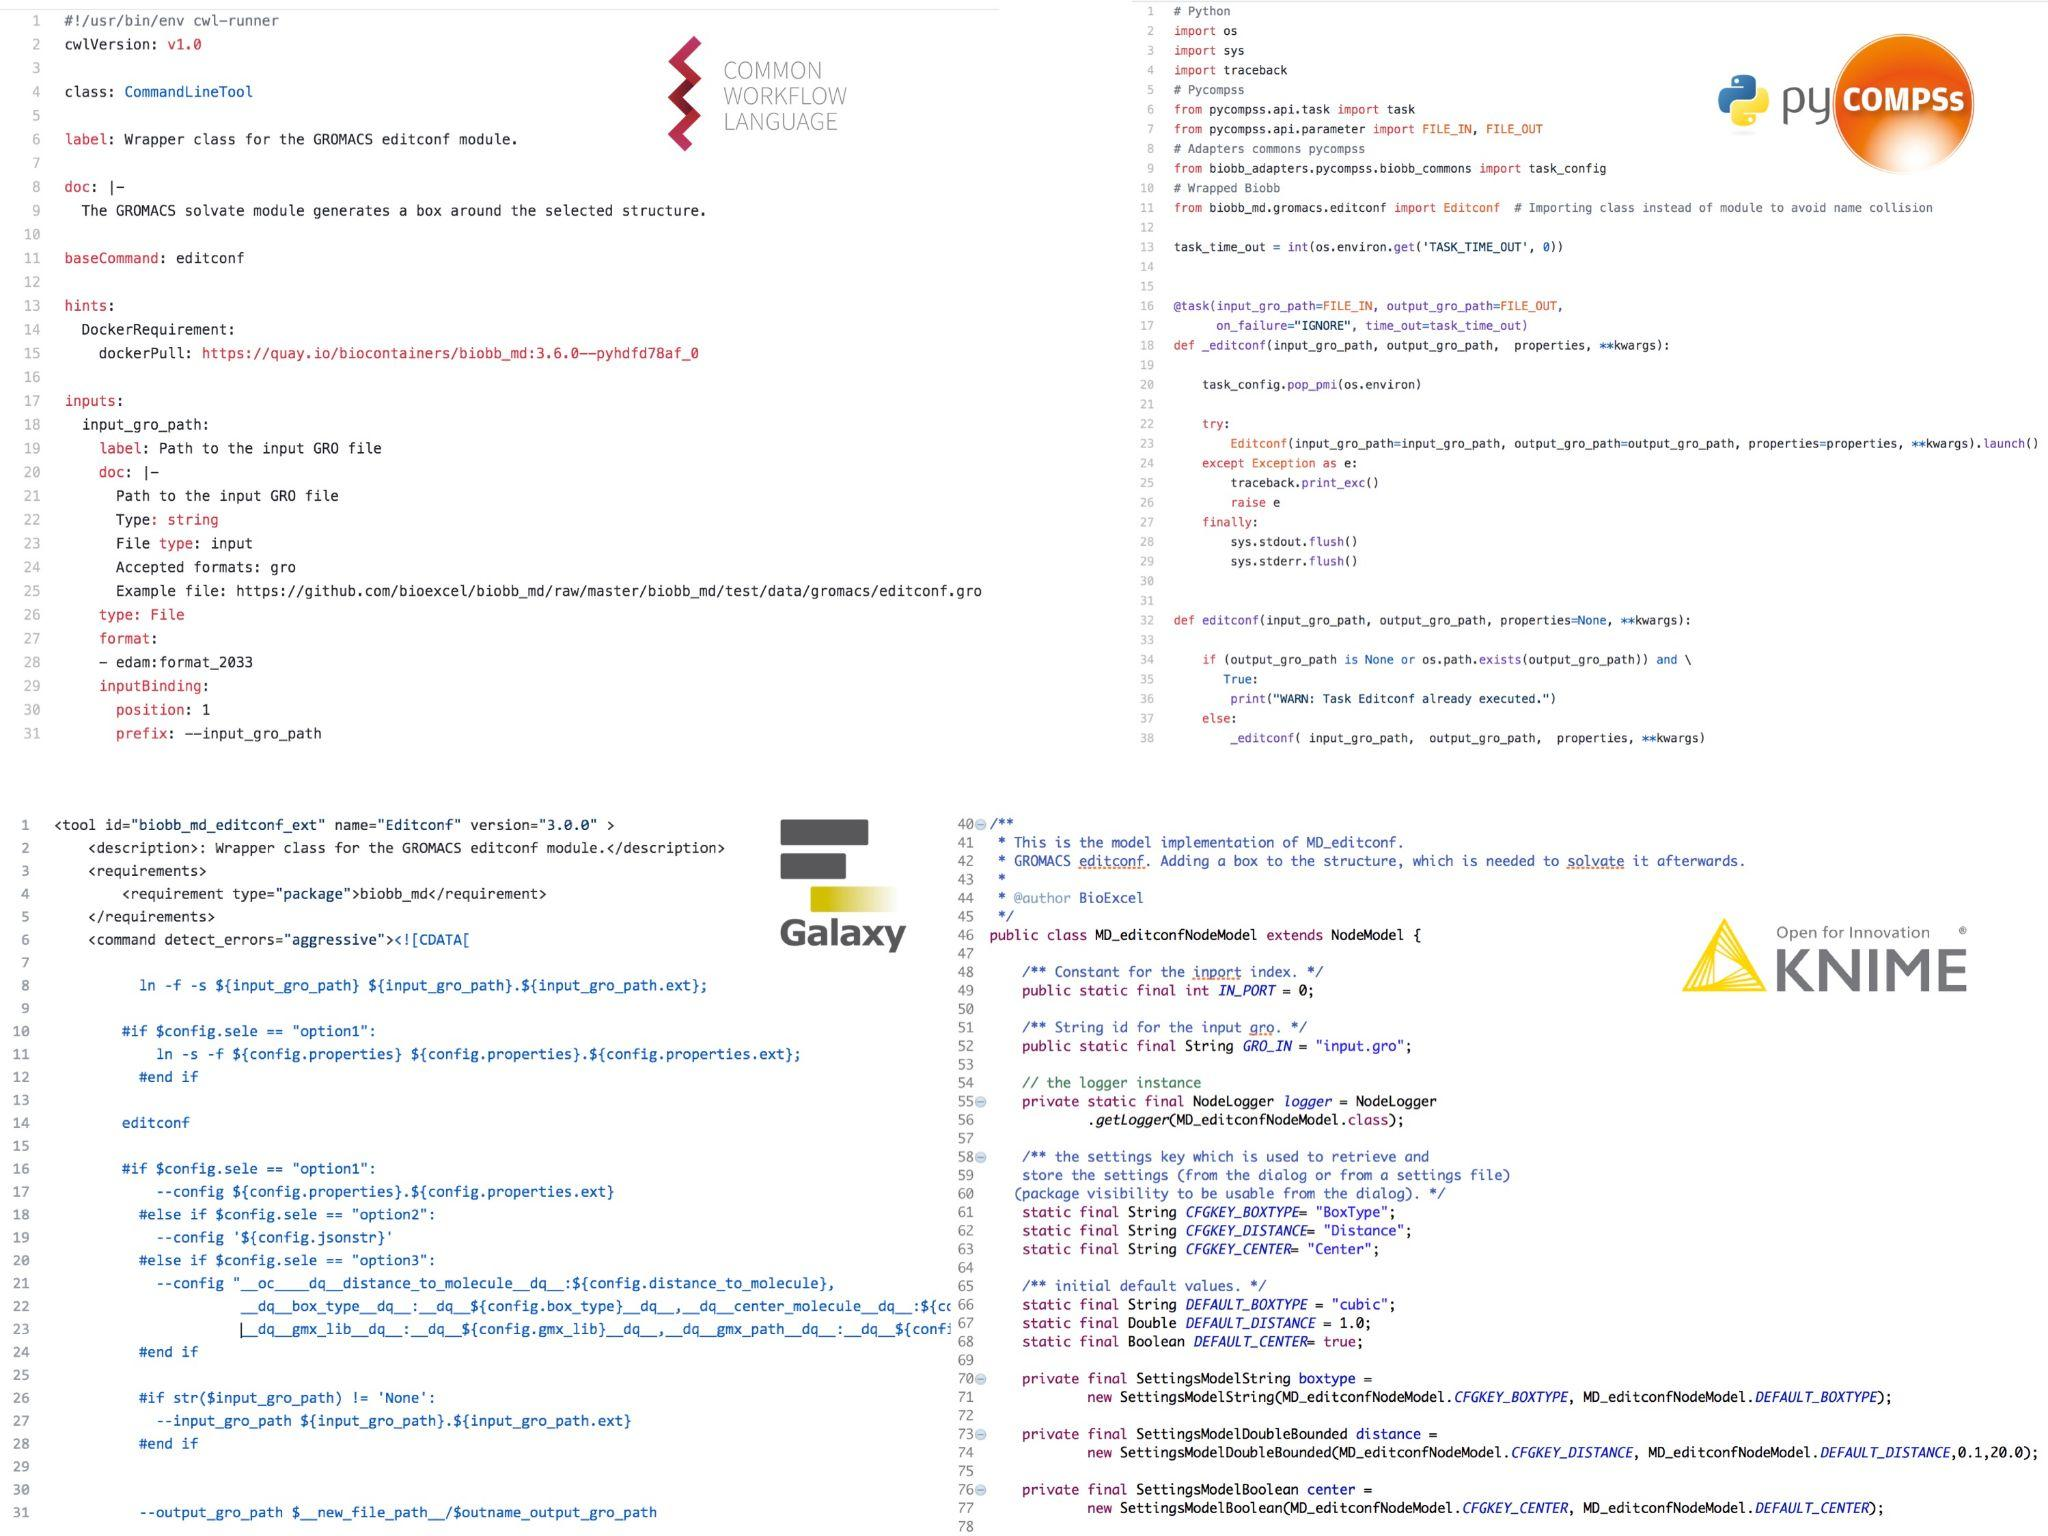
\includegraphics[width=\textwidth]{figures/ch06/figure1.jpg}
	\caption[Code snippets for the BioBB WfMS bindings]{
    \textbf{Code snippets for the BioBB WfMS bindings}: 
    CWL, PyCOMPSs, Galaxy and KNIME.}
  \label{ch6:figure1}
\end{figure}

The library is showcased through a collection of \footurl{http://mmb.irbbarcelona.org/biobb/workflows}{demonstration workflows} \cite{Hospital 2020}.
Here, each workflow introduces individual building blocks as needed to explain a particular scientific computational method.
We primarily expose the workflows as Jupyter Notebooks \cite{Kluyver 2016}, which has been highlighted as a valuable tool for reproducible scientific workflows \cite{Beg 2021}.
This offers a graphical interactive interface, including documentation (integrated markdown) related to the workflow and the building blocks used, but also to the biomolecular simulation methods used in the pipeline.
Moreover, as we have demonstrated with our own \footurl{https://hub-bioexcel-binder.tsi.ebi.ac.uk/}{Binder} \cite{Jupyter 2018} hosting, these workflows are reproducible across platforms, assisted by BioConda \cite{Grüning 2018a} packaging of the building blocks and their software dependencies.

This assembly of available demonstration workflows have been successfully used in the BioExcel CoE for dissemination with a range of \footurl{https://mmb.irbbarcelona.org/biobb/about/training}{training events} 
(e.g.~BioExcel Summer \& Winter School, webinars and virtual training).
In training we particularly utilised the Binder infrastructure of the BioExcel Cloud portal \cite{Niewielska 2020} to give users a web-based first experience of the building blocks before they try them in other workflow systems.

We can observe that workflow building blocks such as BioBB are necessarily composed of a comprehensive list of digital objects, encompassing source code, packaging, containerization, documentation, attributions, citations, registry entries, WfMS integrations and \acrshort{REST} \acrshort{API}s.

We propose to consider building blocks as \emph{composite digital objects} in their own right: gathering the above software components along with their metadata, identifiers and operations then forms a \emph{Canonical Workflow Building Block} (\textbf{CWBB}).
We suggest this concept as a fundamental element of FAIR Digital Objects for Computational Workflows: researchers use the building blocks computationally as functional operations across WfMSs, while the FAIR aspect of CWBB propagates information and resources that are essential for reproducibility, reuse and understanding by anyone discovering the workflow.

\subsubsection{Interoperability across different workflow languages}\label{ch6:interoperability-across-different-workflow-languages}

The concept of Canonical Workflow Building Blocks is here showcased with the BioBB library, by using a transversal workflow present in many different computational biomolecular projects: a \footurl{http://mmb.irbbarcelona.org/biobb/workflows/tutorials/md_setup}{Molecular Dynamics (MD) protein setup}.
This workflow prepares a protein structure to be used as input for an MD simulation, going through a series of steps where the protein is completed (adding hydrogen and missing atoms), optionally introducing a residue mutation, then submerging the protein in a virtual box of water molecules with a particular ionic concentration, and finally energetically equilibrating the system (so that solvent and ions are well accommodated around the protein at the desired temperature).

This simulation process involves a non-negligible number of steps, using a variety of biomolecular tools.
The BioBB library was used to assemble this workflow, interconnecting building blocks using Python functions (Jupyter Notebook, Command Line Interface), auto-generated bindings (Galaxy \cite{Afgan 2018}, CWL \cite{Crusoe 2022}, PyCOMPSs \cite{Tejedor 2017}) or manually generated bindings (KNIME \cite{Fillbrunn 2017}).
Corresponding workflows for the different WfMS can be found in \footurl{https://workflowhub.eu/collections/3}{WorkflowHub} \cite{Lowe 2021a,Hospital 2021b,Bayarri 2021a,Bayarri 2021b,Hospital 2021a} and graphical extracts can be seen in Figure \vref{ch6:figure2}.

This example demonstrates how the same canonical building blocks can be used in different WfMS.
Wrappers and tools executed behind the workflows are exactly the same, but the workflows are built using different WfMS, some of them in a graphical way (drag \& drop, Galaxy, KNIME), some in a command line way (Jupyter Notebook, PyCOMPSs, CWL); workflows can be focused on short/interactive executions (Jupyter Notebook), or on High Throughput/High Performance Computing (HT-HPC) executions (PyCOMPSs); some of them prepared for a particular WfMS installation (Galaxy), others completely system-agnostic (CWL).

The current number of available WfMS bindings include Jupyter Notebook, PyCOMPSs, CWL, Galaxy and KNIME WfMS, in addition to a \footurl{http://mmb.irbbarcelona.org/biobb/availability/tutorials/command-line}{command line} mechanism.
Thanks to the extensive documentation added in the source code as Python docstrings, new bindings for available WfMS can be generated.
We are also experimenting with generating a REST API exposing the building services as Web services.
However, it should be noted that such automatic generation of bindings is not always practically feasible.
As an example, KNIME nodes require a complete Java skeleton code, as well as a definition of new data types for all inputs/outputs required, which makes their automatic generation a heavy and potentially error-prone task.
Bindings for workflow languages with a \emph{domain-specific language} (DSL) for tool definitions (e.g.~Galaxy, CWL) can on the other hand be generated in a more straightforward fashion.

\begin{figure}%[t]
  \centering
  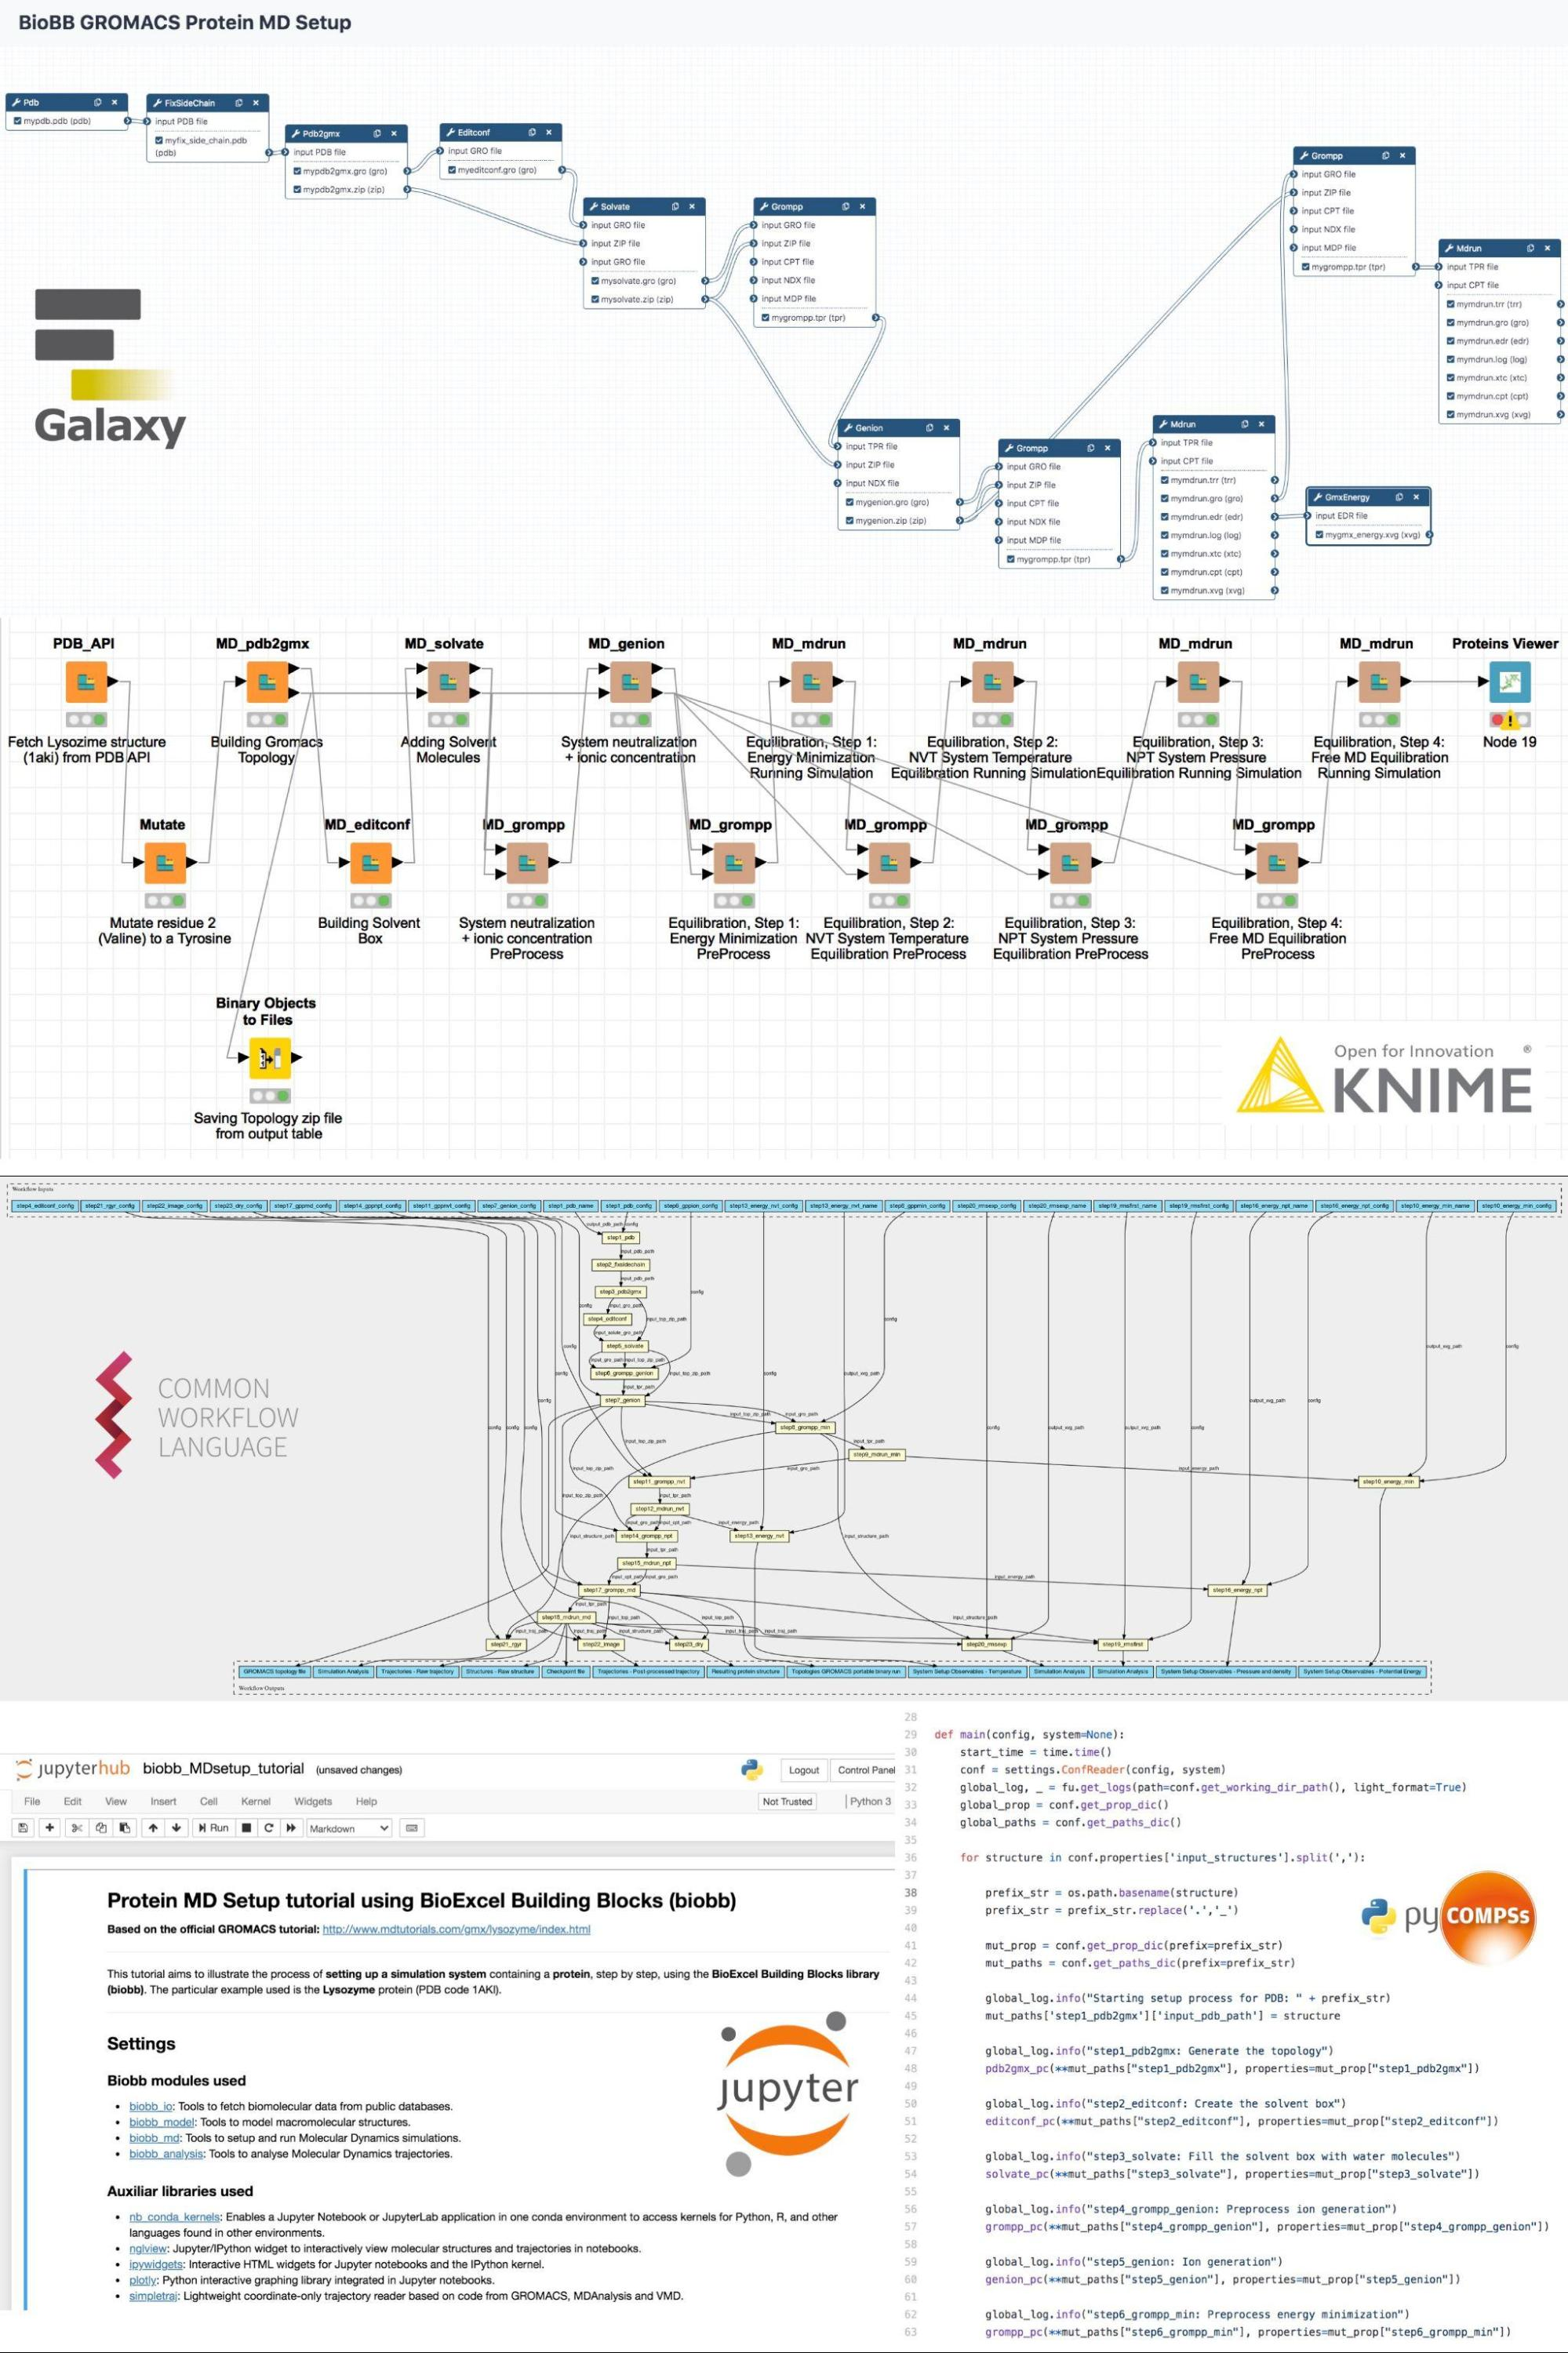
\includegraphics[height=19cm]{figures/ch06/figure2.png}
	\caption[Protein MD Setup transversal workflow]{\textbf{Protein MD Setup transversal workflow}.
Assembled in with 5 different workflow managers using BioBB canonical building blocks.
From top-left: Galaxy \cite{Lowe 2021a}, KNIME \cite{Hospital 2021b}, CWL \cite{Bayarri 2021a}, Jupyter Notebook \cite{Bayarri 2021b}, PyCOMPSs \cite{Hospital 2021a}.}
  \label{ch6:figure2}
\end{figure}

The transversal \footurl{https://workflowhub.eu/collections/3}{protein MD setup workflow} was chosen as a real example that is readily understandable by domain experts.
More \footurl{https://mmb.irbbarcelona.org/biobb/workflows}{complex pipelines} involving a broader set of wrapped biomolecular tools have been developed using the BioBB library, primarily as Jupyter Notebooks.
A selection of these have similarly been assembled for different WfMS using the auto-generated bindings and uploaded to the \footurl{https://workflowhub.eu/projects/11\#workflows}{WorkflowHub repository}.

\subsection{Discussion}\label{ch6:discussion}

Early work on libraries of workflows fragments include Web Service-based approaches where tools are wrapped and exposed using common, interoperable data types in \footurl{http://biomoby.open-bio.org/}{BioMoby} \cite{BioMoby 2008} for bioinformatics and similarly \footurl{https://en.wikipedia.org/wiki/CaBIG}{caBIG} \cite{Saltz 2006} for cancer genomics.
While these efforts were interoperable across WfMSs they required a large up-front investment in agreeing to and adapting native data to common RDF or XML representations.

The notion of \emph{abstract workflows} \cite{Garijo 2011}, structural workflow descriptions separated from their concrete execution realisations and augmented with \acrlong{LD} annotations, have been emphasised as essential for reuse and consistency across workflow systems.
Identifying \emph{common motifs} for workflow operations \cite{Garijo 2014a} (e.g.~Data preparation, Format transformation, Filter, Combine) are important to simplify and understand otherwise fine-grained workflow provenance traces.

Most other efforts to standardise a set of disparate analytical tools have been done within the scope of a single WfMS, allowing customised user interaction, data visualisation, configuration and findability, for instance \footurl{http://www.taverna.org.uk/documentation/taverna-2-x/components/}{Taverna components} had prototypical building blocks \cite{De Giovanni 2016} which were instantiated at runtime by reference from a registry. 
\footurl{https://docs.knime.com/2020-07/analytics_platform_components_guide/index.html}{KNIME components and metanodes}, shared on the \footurl{https://hub.knime.com/}{KNIME Hub} are frequently designed to be interoperable, but with a perhaps weaker notion of component families.
The \footurl{https://toolshed.g2.bx.psu.edu/}{Galaxy toolshed} \cite{Blankenberg 2014} is likewise populated with different sets of tool wrappers that are largely made to be interoperable within a category.

The \emph{Common Workflow Language} (\textbf{CWL}) \cite{Crusoe 2022} has a strong emphasis on interoperable command line tool descriptions, with \footurl{https://www.commonwl.org/user_guide/07-containers/}{support for containers} and Conda packaging, as well as \footurl{https://www.commonwl.org/user_guide/17-metadata/}{support for FAIR metadata} like contributors, license and EDAM ontology type annotations.
With multiple leading workflow engines \footurl{https://www.commonwl.org/implementations/}{now supporting CWL}, and experimental Galaxy support, this seems perhaps the most promising candidate for both making and describing canonical workflow building blocks; however, we have identified a few stumbling blocks.

One obvious challenge is that the implementing WfMS needs to have CWL support, along with support for either containers or Conda packaging to find the described executables.
While it is possible to run a CWL tool directly using a \texttt{\#!/usr/bin/env\ cwl-runner} \footurl{https://en.wikipedia.org/wiki/Shebang_(Unix)}{shebang} on POSIX systems, this still requires pre-installation and possibly configuration of a CWL engine like \footurl{https://pypi.org/project/cwltool/}{cwltool} or \footurl{https://toil.readthedocs.io/en/latest/running/cwl.html}{Toil} \cite{Vivian 2017}.
However workflow engines have multiple dependencies and often cannot easily be run from a container themselves\footnote{To execute the wrapped tool, a containerised workflow engine would need \emph{nested containers} which are not generally recommended for security reasons.
It is possible to work around this limitation using \emph{Singularity} (\url{https://sylabs.io/singularity/}) or \emph{Conda} (\url{https://docs.bioexcel.eu/cwl-best-practice-guide/devpractice/containers/conda.html}).}.

Within the CWL community it was originally envisioned that a wider set of workflow systems would adopt CWL for tool description/execution, with a subset implementing full CWL workflow support.
This would allow shared community effort for describing tools, say in the \footurl{https://github.com/common-workflow-library/}{Common Workflow Library}, rather than each WfMS needing to duplicate this tool wrapping in separate repositories and languages.
However, with the exception of experimental tool support in Galaxy, in practice all CWL implementers have gone for full workflow support.

Another challenge is that making a set of building blocks frequently requires the use of \emph{shims}, for instance file conversion, small search/replace operations or file renames.
In a CWL approach these can either be performed with an \footurl{https://www.commonwl.org/v1.2/Workflow.html\#Expressions_(Optional)}{Expression} using JavaScript snippets which only has limited access to file content, or as an additional workflow step added before or after the main tool step.
This combination could then be nested as a subworkflow, similar to KNIME's \emph{metanodes}, and would also be flexible by allowing different containers or packages for any pre- or post-steps.
Such a CWL building block, however, becomes harder to access from a non-CWL WfMS, because of lack of control over configuration/execution options for the
now nested CWL tools.
In practice\footnote{It is worth mentioning that it would also be possible to generate WfMS-specific bindings from CWL descriptions 
(e.g.~as demonstrated with 
cwl2script (\url{https://github.com/common-workflow-lab/cwl2script}) for Bash, 
gxargparse (\url{https://github.com/common-workflow-lab/gxargparse}) for Galaxy, 
cwl2wdl (\url{https://github.com/common-workflow-lab/cwl2wdl}) for WDL), 
although this necessitates constraining the tool and workflow definitions to a limited mappable subset of CWL.}, executing a nested CWL workflow from a native WfMS language would require the engine to implement full CWL Workflow support (or delegate to a CWL engine).

For the main BioBB building blocks we implemented \footurl{http://mmb.irbbarcelona.org/biobb/workflows}{demonstrator workflows} that highlight how the tools should be used in different workflow management systems; each having a primary exemplar using Jupyter Notebook, which can be explored interactively using the \footurl{https://hub-bioexcel-binder.tsi.ebi.ac.uk/h}{BioExcel Binder}.
If we consider the abstract demonstrator workflows as \emph{canonical workflows} they are therefore very much active objects, but can also be seen as \emph{workflow templates}, as any real use case will need to specialise the workflow to tweak parameters, data selection etc.

We therefore also provide such workflow templates for multiple WfMS, including CWL, PyCOMPSs and Galaxy.
These are fairly disparate workflow languages, yet by the use of the same canonical workflow building blocks (which again invoke the same software binaries), such WfMS-specific workflows effectively are instantiations of the same canonical workflow.

One challenge found is how to publish such canonical workflows in registries like the \footurl{https://workflowhub.eu/}{WorkflowHub}.
The hub supports the registration of Digital Objects in the form of \acrshort{RO-Crate} \cite{Soiland-Reyes 2022a}, with the option of abstract CWL for describing the canonical workflow template, along with direct references to the workflow's GitHub repository.

\clearpage % footnotes explode otherwise!
For instance in the RO-Crate for \url{https://doi.org/10.48546/workflowhub.workflow.200.1} \cite{Hospital 2021a}, which can also be
\footurl{https://rawcdn.githack.com/bioexcel/biobb_hpc_workflows/53958e7c278e53c277a7217057b785482f193f7f/ro-crate-preview.html}{rendered} from GitHub, we have an entry for the 
\footurl{https://rawcdn.githack.com/bioexcel/biobb_hpc_workflows/53958e7c278e53c277a7217057b785482f193f7f/ro-crate-preview.html\#workflows/MD/md_list.py}{\emph{main workflow}}
according to the
\footurl{https://w3id.org/workflowhub/workflow-ro-crate/1.0}{Workflow RO-Crate profile}, 
detailing each canonical workflow building block used 
(e.g.~\footurl{https://rawcdn.githack.com/bioexcel/biobb_hpc_workflows/53958e7c278e53c277a7217057b785482f193f7f/ro-crate-preview.html\#https\%3A//pypi.org/project/biobb-md/3.6.0/}{biobb-md metadata}).
Here the FAIR aspect of the building blocks to help software citation is exercised, as the building block wrapper has one set of authors, documentation and licence (Apache-2.0), while the wrapped software 
(e.g.~\footurl{https://rawcdn.githack.com/bioexcel/biobb_hpc_workflows/53958e7c278e53c277a7217057b785482f193f7f/ro-crate-preview.html\#https\%3A//doi.org/10.5281/zenodo.2564764}{GROMACS metadata})~has different authors, licence (GPL-2.1+) and documentation.

However, the deposit of such RO-Crates in WorkflowHub results in one registration entry per workflow language, which are not otherwise related and may not even share the same source code repository.
Thus, we have identified the need for adding an overall \emph{canonical workflow entry}, which can bring in workflow documentation and references shared across WfMS implementations, including a set of links to the more granular canonical workflow building blocks used by the workflow, but also to the individual WfMS implementations as separate digital objects.

A similar question of granularity applies at the workflow tool level \cite{Möller 2017}, particularly for Findability and Accessibility, as we can consider at lowest granularity the \emph{scientific method} in general (e.g.~any algorithm for sequence alignment), followed by an \emph{application suite} (bio.tools entry \cite{Ison 2021}, homepage, documentation), instantiated as a particular \emph{software installation} (Debian package, Docker container) with its dependencies at same level.
The installation includes one or more \emph{software executables} (a particular binary, a running service service), providing at the highest detailed granularity level the specific types of \emph{software functionality} (a particular mode of operation, choice of analysis), for instance using certain command line flags.

For canonical workflow building blocks, with a focus on pluggable composability, this is mainly defined at this high granularity level of specific software functionality: explicit operations from an installed tool, which are then combined in a workflow.
This is indeed the level WfMS tool definitions are typically done, e.g.~a CWL Command Line Tool specifies a particular way to run a particular software binary.
However, to be an actionable CWBB, the building block needs to additionally convey the lower granularity levels; particularly to support multiple options for interoperable installation and execution, as well as metadata at the most general level, such as documentation and scholarly citations.

While workflow management systems typically only operate at the highest granularity levels for execution details, and are frequently unaware of (or not exposing metadata at) the more general levels, we argue that in order for a Canonical Workflow \cite{CWFR 2021} to follow and support FAIR principles for itself and its data, the workflow management system need to \emph{propagate structured metadata} about the tools used by the workflow.
We propose that in order to support the workflow's applicability to multiple WfMS, the tools themselves must also have a consistent packaging and formal description that enables consistent computational invocation.

At the most general level, a canonical workflow built using such CWBBs is even conceptually reproducible because the FAIR documentation of the workflow, through its canonical workflow building blocks, identifies how individual tools and software applications are composed, which in worst case can be rebuilt using different installation methods in a different WfMS, or in best case inspected to detect and cross-link the same canonical workflow appearing in different WfMS instantiations.
This view of software as composition of other software typically also applies at individual tool level, which themselves depend on programming language runtimes, libraries, services and reference data.

\subsection{Requirements for Canonical Workflow Building Blocks}\label{ch6:requirements-for-canonical-workflow-building-blocks}

Building on the experiences with BioBB, we here propose requirements and recommendations for establishing Canonical Workflow Building Blocks (CWBB) as implementations of \emph{canonical steps} introduced for Canonical Workflow Frameworks for Research \cite{CWFR 2021}.

The core purpose of a CWBB is to wrap a command line tool or other software that can perform an operation as part of a computational workflow.
As such, the general advice for making software workflow-ready applies \cite{Brack 2022a} (e.g.~easy to install, documented, parallelizable, reproducible output); however, a CWBB is also permitted to make use of additional scripts or \emph{shims} to further adapt a third-party tool for workflow use and for data interoperability across blocks.

The way tools are installed or invoked varies slightly across WfMS and operating systems, therefore a CWBB should provide multiple methods for distributing software; currently containers (Docker, Singularity) and distribution-independent packaging (e.g.~Conda, Homebrew) are promising by having reproducible install recipes and a wide range of open source dependencies (e.g.~Java, Python).
Additionally building blocks should allow overriding execution paths, e.g.~for use with HPC module system and hardware-optimised binaries.

The CWBBs should have sufficient annotations to be able to generate bindings for different WfMSs and REST APIs, e.g.~parameter names and descriptions, types and default values; enumerators for options, file formats for inputs/outputs.

Building blocks should be grouped into families that are interoperable through common data structures and file formats, as well as having joint naming conventions for configuration options.
A CWBB family should be released as a single version following \footurl{https://semver.org/spec/v2.0.0.html}{semantic versioning} rules, which should have a corresponding persistent identifier (PID) \cite{McMurry 2017}.

Metadata for CWBBs should be captured following FAIR guidelines, and distributed as part of the block family and resolvable from the PID as a FAIR Digital Object.
Metadata should include references to the CWBB software distributions (e.g.~\footurl{https://quay.io/search}{quay.io} container URL) as well as attributions, citations and documentation for the wrapped tool.

Example workflows showing CWBB usage should be included in a WfMS-neutral language such as Jupyter Notebooks, which may have equivalent variants for each workflow binding.
These workflows should be registered in a workflow registry like WorkflowHub or Dockstore, and assigned their own PIDs.

\subsection{Conclusions}\label{ch6:conclusions}

The proposed concept of Canonical Workflow Building Blocks can bridge the gap between FAIR Computational Workflows, interoperable reproducibility and for building canonical workflow descriptions to be used and described FAIRly across WfMSs.

The realisation of CWBBs can be achieved in many ways, not necessarily using the Python programming language together with RO-Crate as explored here.
In particular if the envisioned Canonical Workflow Frameworks for Research become established in multiple WfMSs with the use of FAIR Digital Objects, the different implementations will need to agree on object types, software packaging and metadata formats in order to reuse tools and provide interoperable reproducibility for canonical workflows.

Likewise, to build a meaningful collection of building blocks for a given research domain, a directed collaborative effort is needed to consistently wrap tools for a related set of WfMSs, chosen to target particular use cases (a family of canonical workflows).

For individual users, a library of Canonical Workflow Building Blocks simplifies many aspects of building pipelines, beyond the FAIR aspects and data compatibility across blocks.
For instance, they can benefit from training of a CWBB family using Jupyter Notebooks, and then use this knowledge to utilise the same building blocks in a scalable HPC workflow with a CWL engine like Toil, knowing they will perform consistently thanks to the use of containers.

While we have demonstrated CWBB in the biomedical domain, this approach is generally applicable to a wide range of sciences that execute pipelines of multiple file-based command line tools -- however, it may be harder to achieve with more algebraic ``in memory'' types of computational workflows, where steps could be challenging to containerize and distinguish as separate block.

We admit that biomolecular research is quite a homogenous field with respect to computational analyses and now becoming relatively mature in terms of tool composability in workflows, building on the experiences of the ``FAIR pioneers'' in the field of bioinformatics.
Other fields, such as social sciences or ecology, can have a wider variety of methods and computational tools, often with human interactions, and may have to adapt the software to be workflow-ready \cite{Brack 2022a} before using them as Canonical Workflow Building Blocks.
Domains adapting CWBB approach (or workflow systems in general) should take note of the great benefits of hosting collaborative events where developers meet each other and their potential users, demonstrated in our field with events such WorkflowsRI \cite{Ferreira da Silva 2021} and Biohackathons \cite{Garcia 2020}.

The Common Workflow Language shows promise as a general canonical workflow building blocks mechanism: gathering execution details of tools along with their metadata and references, augmented with \footurl{https://docs.bioexcel.eu/cwl-best-practice-guide/devpractice/partial.html\#using-abstract-operations-as-placeholders}{abstract workflows} to represent canonical workflows.
However, this would need further work to implement our CWBB recommendations in full.
Future work for the Canonical Workflow Building Blocks concept includes formalising and automating publication practises, to make individual blocks available as FAIR Digital Objects on their own or as part of an aggregate collection like RO-Crate.

\section{The Specimen Data Refinery}
\label{ch8:the-specimen-data-refinery}

\subsection*{A canonical workflow framework and FAIR Digital Object
approach to speeding up digital mobilisation of natural history
collections}

A key limiting factor in organising and using information from physical
specimens curated in natural science collections is making that
information computable, with institutional digitization tending to focus
more on imaging the specimens themselves than on efficiently capturing
computable data about them. Label data are traditionally manually
transcribed today with high cost and low throughput, rendering such a
task constrained for many collection-holding institutions at current
funding levels.

We show how computer vision, optical character recognition, handwriting
recognition, named entity recognition and language translation
technologies can be implemented into canonical workflow component
libraries with findable, accessible, interoperable, and reusable (FAIR)
characteristics. These libraries are being developed in a cloud-based
workflow platform -- the `Specimen Data Refinery' (SDR) -- founded on
Galaxy workflow engine, Common Workflow Language, Research Object Crates
(RO-Crate) and WorkflowHub technologies. The SDR can be applied to
specimens' labels and other artefacts, offering the prospect of greatly
accelerated and more accurate data capture in computable form.

Two kinds of FAIR Digital Objects (FDO) are created by packaging outputs
of SDR workflows and workflow components as digital objects with
metadata, a persistent identifier, and a specific type definition. The
first kind of FDO are computable Digital Specimen (DS) objects that can
be consumed/produced by workflows, and other applications. A single DS
is the input data structure submitted to a workflow that is modified by
each workflow component in turn to produce a refined DS at the end. The
Specimen Data Refinery provides a library of such components that can be
used individually, or in series. To cofunction, each library component
describes the fields it requires from the DS and the fields it will in
turn populate or enrich. The second kind of FDO, RO-Crates gather and
archive the diverse set of digital and real-world resources,
configurations, and actions (the provenance) contributing to a unit of
research work, allowing that work to be faithfully recorded and
reproduced.

Here we describe the Specimen Data Refinery with its motivating
requirements, focusing on what is essential in the creation of canonical
workflow component libraries and its conformance with the requirements
of an emerging FDO Core Specification being developed by the FDO Forum.

\subsection{Introduction}\label{introduction-2}

A key limiting factor in organising and using information from physical
specimens curated in natural history collections is making that
information computable (`machine-actionable') and extendable. More than
85\% of available information currently resides on labels attached to
specimens or in physical ledgers \cite{Walton 2020}. Label data are commonly
transcribed manually with high cost and low throughput, rendering such a
task constraining for many institutions at current funding levels.
However, the advent of rapid, high-quality digital imaging has meant
that digitizing specimens, including their labels, is now faster and
cheaper \cite{ch8-2}. With initiatives such as Advancing Digitization of
Biological Collections (ADBC), integrated Digitized Biocollections
(iDigBio) and the Distributed System of Scientific Collections (DiSSCo)
\cite{ch8-3,ch8-4,ch8-5,ch8-6} aiming to increase the rate and accuracy of both mass and
on-demand digitization of natural history collections, the gap between
expectations of what should be digitally available and computable, and
what can be achieved using traditional transcription approaches is
widening. Modern, highly efficient workflow tools and approaches can
play a role to address this.

Collection digitization began towards the end of the 20th century by
typing basic data from labels into the collection (asset) management
systems of collection-holding institutions such as natural history
museums, herbaria and universities. Initially, this was to facilitate
indexing and cataloguing and locating the physical specimens, but with
the addition of photographic images of specimens and the public
availability of specimen data records, through data portals of the
institutions themselves as well as international data infrastructures
like the Global Biodiversity Information Facility (GBIF), such bodies of
data have been rapidly exploited for research \cite{ch8-7,ch8-8}. It has become
clear that widespread digitization of data about physical specimens in
collections and the advent of high-throughput digitization processes
\cite{ch8-9,ch8-10,ch8-11,ch8-12,ch8-13} is transforming and will radically further transform the
range of scientific research opportunities and questions that can be
addressed \cite{ch8-14,ch8-15}. Scientific conclusions and policy decisions
evidenced by digital specimen data enhance humankind's ability to
conserve, protect, and predict the biodiversity of our world
\cite{ch8-16,ch8-17}.

Harnessing technologies developed to harvest, organise, analyse and
enhance information from sources such as scholarly literature,
third-party databases, data aggregators, data linkage services and
geocoders and reapplying these approaches to specimens' labels and other
artefacts offers the prospect of greatly accelerated data capture in a
computable form \cite{ch8-18}. Tools of particular interest span the fields
of computer vision, optical character recognition, handwriting
recognition, named entity recognition and language translation.

Workflow technologies from the ELIXIR Research Infrastructure \cite{ch8-19},
including Galaxy \cite{Afgan 2018}, Common Workflow Language \cite{Crusoe 2022}, Research
Object Crates (RO-Crates) \cite{OCarragain 2019,Soiland-Reyes 2022} and WorkflowHub \cite{Goble 2021}, and
selected tools are integrated in a cloud-based workflow platform for
natural history specimens -- the `Specimen Data Refinery' \cite{Walton 2020} that
will become one of the main services to be offered by the planned DiSSCo
research infrastructure \cite{ch8-5}. The tools themselves, implemented with
findable, accessible, interoperable, and reusable (FAIR) characteristics
\cite{Wilkinson 2016} are packaged into canonical workflow component libraries
\cite{ch8-27}, rendering them reusable, and interoperable with one another.
FAIR Digital Objects are adopted as the common input/output pattern,
fully compatible with digital objects at the core of DiSSCo data
management \cite{ch8-28}.

The Refinery brings together domain-specific workflows for processing
specimen images and extracting text and data from images with canonical
forms for components and interactions between components that can lead
to improved FAIR characteristics for both the workflows themselves and
the data resulting from workflow execution.

FAIR Digital Objects (FDO) are created by packaging outputs of workflows
and workflow components as digital objects with metadata, a persistent
identifier, and a specific type definition against which operations can
be executed \cite{De Smedt 2020}. The Refinery uses two kinds of FDOs:

\begin{itemize}
\item
  \textbf{computable Digital Specimen (DS) objects} \cite{ch8-30} from DISSCo
  for the scientific input/output data that can be consumed/produced by
  workflows and other applications.
\item
  \textbf{workflow objects, implemented as RO-Crates} \cite{Soiland-Reyes 2022}, from
  ELIXIR gather and archive the diverse set of workflow process data --
  the digital and real-world resources, configurations and actions (the
  provenance) contributing to a unit of digitization or other work
  producing the Digital Specimen digital objects, allowing that work to
  be scrutinised and faithfully reproduced if necessary.
\end{itemize}

We first summarise related work before describing the problem to be
addressed by the Specimen Data Refinery. We then explain our Canonical
Workflows for Research (CWFR) approach using these FDOs in the design of
the SDR, the experimental setup, and results so far from the work in
progress. While future work will clarify full results and challenges of
implementing a robust, reliable, and easy-to-use production-capability
SDR, in this early report following SDR prototyping and
conceptualization, we focus on what we found to be essential in the use
of FDOs and CWFR canonical step libraries, and on the compliance of
canonical workflow (component) inputs and outputs with the requirements
of the FDO Framework \cite{bonino2019}.

\subsection{Related Work}\label{related-work}

\subsubsection{Workflows for processing specimen images and extracting data}\label{workflows-for-processing-specimen-images-and-extracting-data}

While natural history collections are heterogeneous in size and shape,
often they are mass digitized using standardised workflows \cite{ch8-9,ch8-10,ch8-11,ch8-12,ch8-13}.
In pursuit of higher throughput at lower cost, yet with higher accuracy
and richer metadata, further automation will increasingly rely on
techniques of object detection and segmentation, optical character
recognition (OCR) and semantic processing of labels, and automated
taxonomic identification and visual feature analysis \cite{Walton 2020,ch8-18}.

Although there is a great deal of variety among images of different
kinds of collection objects that are digitized (see Figure \vref{ch8:figure1}) there are
visual similarities between them. Most images contain labels, scale bars
and often, colour charts as well as the specimen itself. This makes them
amenable to improved approaches to object detection \cite{ch8-32} and
segmentation into `regions of interest' \cite{ch8-33} as precursive steps for
multiple kinds of workflows.

%% Evil footnotes again
\begin{figure}%[t]
  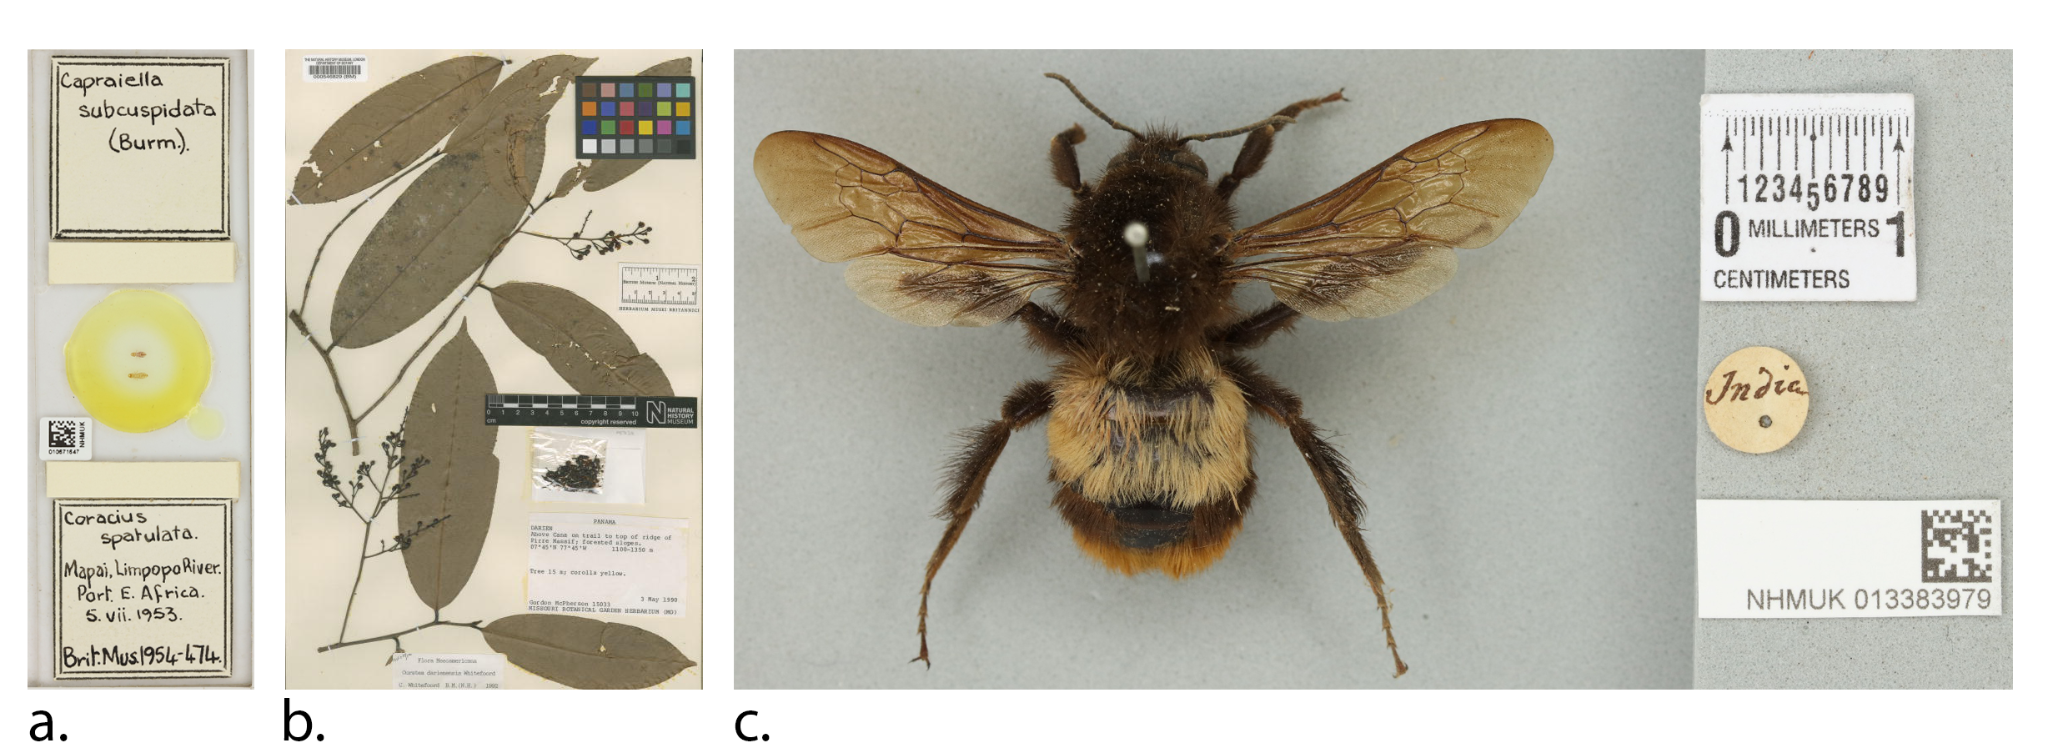
\includegraphics[width=\textwidth]{figures/ch08/figure1.png}
	\caption[A range of specimen images]{\textbf{A range of specimen images}. From the Natural History Museum, London, demonstrating the
  diversity of collection objects, which include handwritten, typed, and
  printed labels. (a) Microscope slide (NHMUK010671647)\footnotemark{},
  (b) Herbarium specimen (BM000546829)\footnotemark{},
  (c) pinned insect (NHMUK013383979)\footnotemark{}.}
  \label{ch8:figure1}
\end{figure}

% Evil goes her
\addtocounter{footnote}{-3}
\addtocounter{footnote}{1}\footnotetext{\url{https://data.nhm.ac.uk/object/c65d9a3c-d8f6-4fac-a418-05c3b697cece}}
\addtocounter{footnote}{1}\footnotetext{\url{https://data.nhm.ac.uk/object/be595f07-73c5-4764-a96c-8b377e3d1507}}
\addtocounter{footnote}{1}\footnotetext{\url{https://data.nhm.ac.uk/object/745febc7-8222-498a-9969-5f6b12f85ef3}}
%%

Segmentation, specifically, can be employed as an early step in a
workflow to send just the relevant region(s) of interest from an image
to later workflow steps. Not only does this decrease data transfer time
and minimise computational overheads but it can also substantially
increase the accuracy of subsequent OCR processing and semantic
recognition steps \cite{ch8-18}.

Much of the data about specimens is stored on their handwritten, typed
or printed labels or in registers/ledgers \cite{ch8-34}. Direct manual
transcription into local databases with manual georeferencing is the
primary method used today to capture this data. Potentially, OCR can
significantly increase transcription speeds whilst reducing cost;
although it sacrifices accuracy and disambiguation that are today
achieved with specialist knowledge provided by humans during the
process. Returning character strings from OCR is useful, but
semantically placing this data in its context as information specific to
natural history specimens and linking that back to the original physical
specimens is of much higher value, improving the utility of natural
history collections. Shortfalls in accuracy and disambiguation can be
made up by exploiting Natural Language Processing (NLP) advances such as
named entity recognition to identify text segments belonging to
predefined categories (for example, species name, collector, locality,
date) \cite{ch8-18}. Nevertheless, this only works well on a small proportion
of captured data in the absence of `human in the loop' input. To better
automate disambiguation of people's names, for example, access to other
contextual `helper' data are needed (e.g., biographical data in
Wikidata) as well as cross-comparison with other data from the specimen,
such as the date of collection and location \cite{ch8-35}.

Automated identification of species from images of living organisms has
achieved impressive levels of accuracy 
\cite{ch8-36,ch8-37,ch8-38,ch8-39,ch8-40,ch8-41} with techniques
translated to an increasing range of enthusiastically received consumer
applications for plant and animal identification using mobile phones
(e.g., \footurl{https://www.plantsnap.com/}{Plantsnap},
\footurl{https://www.picturethisai.com/}{PictureThis},
\footurl{https://www.inaturalist.org/pages/seek_app}{iNaturalist SEEK}).
Automated identification of \emph{preserved specimens}, however,
presents different challenges. Although identification might be made
more accurately because a specimen is presented in a standard manner,
separated from other organisms and the complexity of a natural
background, the loss of colour and distortion of the shape of the
organism arising from preparation and preservation processes can lead to
the loss of important identification clues that might be present on a
living example.

\subsubsection{Workflow management systems and canonical workflows
for
research}\label{ch8:workflow-management-systems-and-canonical-workflows-for-research}

A workflow chains together atomised and executable components with the
relationships between them to clearly define a control flow and a data
flow. Their significant defining characteristics are (i) abstraction,
through the separation of the workflow specification (the work to be
done) from its execution (how it is done), and (ii) composition whereby
the components can be cleanly combined and reused and workflows
themselves can be neatly packaged as components \cite{Atkinson 2017}. Workflow
management systems typically provide the necessary mechanisms for
explicitly defining workflows in a reusable way together with a workflow
engine that executes the workflow steps and keeps an accountable record
of the processing -- logging the codes executed and the data lineage of
the results. In the past decade there has been a rise in popularity in
both the development of WfMS and their use, driven by the increasing
scales of data and the accompanying complexity of its processing
\cite{Atkinson 2017}.

Workflow management systems typically vary in the features they provide
for supporting: workflow programming language and control flow
expressivity; data type management; code wrapping, containerisation and
integration with software management tools; exploitation of
computational architectures; availability of development and logging
tools; licensing and so on. Although several hundred kinds of such
systems exist \cite{ch8-43}, communities tend to cluster around a few popular
systems based on their ``plugged-in'' availability of data type
specialist codes, the catered-for skills level of the workflow
developers, and its documentation, community support and perceived
sustainability. For the Specimen Data Refinery, the Galaxy workflow
system \cite{Afgan 2018} in conjunction with Common Workflow Language (CWL)
\cite{Crusoe 2022} has been chosen. CWL is a workflow specification standard
geared towards supporting interoperable and scalable production
pipelines, abstracting away from the internal data structures of some of
the language-specific workflow systems.

Originally designed for computational biology and with many available
tool components, Galaxy \cite{Afgan 2018} supports multiple domains. Workflows
can be built by manually experimenting with data manipulations in a
`data playground' and subsequently converting histories of those to
workflows, or by a more traditional drag-and-drop composition approach.
New components can be created by wrapping existing programs, with
in-built dependency management and automated conversion to executable
containers. As such, Galaxy and CWL offer possibilities for a rich
canonical workflow component landscape with a workflow management regime
that can be both easily FAIR compliant and efficient internally
\cite{ch8-27}. The WorkflowHub, which facilitates CWL and enables workflows
to be registered, shared and published, is mutually coupled with Galaxy
so that workflows can be discovered in the Hub and immediately executed
in a public-use Galaxy instance.

In the context of the SDR, users can construct institution or
project-specific variants of digitization workflows to suit their
specific needs. As collections are heterogeneous, different specimen
types or specific sets of specimens are likely to have variations and
idiosyncrasies in the digitization and processing needed. Tools for
automated identification of specimens are likely to be taxon-specific,
and as such it seems likely that taxon-specific workflows will become
common. In addition, institutions have specific data exchange
requirements for their individual collection management systems.
Ensuring that workflows can be easily modified in a common environment
bridges the gap between community contribution to shared tooling and the
bespoke needs of specific institutions/collections.

Although computational workflows typically emphasize scalable automated
processing, in practice many also combine automation with manual steps.
This feature is also supported by Galaxy and CWL, allowing (for example)
manual geocoding and verification during the digitization process of the
locations where specimens were collected.

\subsubsection{FAIR Digital Objects}\label{fair-digital-objects-1}

Galaxy/CWL environments offer the possibility to integrate generic
digital object methods \cite{ch8-44,ch8-45,Kahn 2006} for the interactions between
workflow components, thus making them able to meet the need and ease the
burden of compiling FAIR compliant data throughout the research
lifecycle \cite{ch8-27}.

A digital object exhibiting FAIR characteristics is a FAIR Digital
Object \cite{De Smedt 2020} and is defined formally as ``a unit composed of data
and/or metadata regulated by structures or schemas, and with an assigned
globally unique and persistent identifier (PID), which is findable,
accessible, interoperable and reusable both by humans and computers for
the reliable interpretation and processing of the data represented by
the object''.

Supporting `FAIRness' internally and acting as glue between the steps of
canonical workflows, FDOs record and can represent the state of a
workflow, its inputs and outputs, and the component steps performed in a
comprehensive manner \cite{ch8-27}. Each FDO is anchored by a globally unique
and resolvable, persistent identifier (PID) (such as a DOI®, for
example) that clearly refers to one digital entity. The PID resolution
offers persistent references to find, access and reuse all information
entities that are relevant to access and interpret the content of an
FDO. In doing so, the FDO creates a new kind of machine-actionable,
meaningful and technology independent unit of information. This is both
immediately available and amenable for further use, as well as being
comparable to the role of the classical archival storage box when
necessary.

\paragraph{Computable Digital Specimens as a kind of FAIR Digital Object}\label{computable-digital-specimens-as-a-kind-of-fair-digital-object}

Digital Specimens (DS) are a specific class of FDO that group, manage
and allow processing of fragments of information relating to physical
natural history specimens. On a one-to-one correspondence a DS
authoritatively collates data about a physical specimen (i.e.,
information extracted and captured from labels by digitization
workflows) with other data -- often to be found from third-party sources
-- derived from analysis and use of the specimen.

openDS \cite{ch8-47} is the developing specification for open Digital
Specimens and other related object types, defining: 

\begin{itemize}
  \item The logical
  structure and content of Digital Specimen (DS), Basic Image Object (BIO)
  and other object types, and the operations permitted on them.
  \item The
  handling rules and behaviors governing digital specimen object
  operations in general.
  \item Serialization and packaging as
  JavaScript Object Notation (JSON) for lightweight data interchange
  between systems, sub-systems and components of systems (for which, read
  `workflow components' \cite{ch8-48}. 
\end{itemize}

openDS is essential to future FAIR
digitization of natural history collections and to Digital Specimens as
self-standing digital objects on the Internet, amenable to computer
processing. It contributes to the new transformative generation of FAIR
infrastructure and applications based on Digital Object Architecture
that is planned for the Distributed System of Scientific Collections
(DiSSCo) \cite{ch8-6,ch8-5,ch8-30} European research infrastructure.

Henceforth we refer to these as \textbf{openDS FDOs}.

\paragraph{FAIR packaging of research/workflow objects with RO-Crate}\label{ch8:fair-packaging-of-researchworkflow-objects-with-ro-crate}

The useful outcomes of research are not just traditional publications
nor data products but everything that goes into and supports an
investigative work or production pipelining activity. This includes
input and intermediate data, parameter settings, final outputs, software
programs and workflows, and configuration information sufficient to make
the work reproducible. Research objects \cite{Bechhofer 2013} are a general approach
to describing and associating all of this content together in a
machine-readable form so that it can be easily preserved, shared and
exchanged. Workflow objects are a specific subclass of research objects.

RO-Crate\footnote{Chapter \vref{ch5:packaging-research-artefacts-with-ro-crate}} \cite{OCarragain 2019,Soiland-Reyes 2022} has been established as a community standard to
practically achieve FAIR packaging of research objects with their
structured metadata. Based on well-established Web standards, RO-Crate
uses JSON-LD \cite{w3-json-ld} with \cite{schema.org} for its common metadata representation. It is extensible with
domain-specific vocabularies in a growing range of specializing RO-Crate
profiles, e.g., for domains such as earth sciences \cite{ch8-52}, biosciences
\cite{Goble 2021}; for object types such as data or workflow \cite{Bacall 2022}; or for
workflow runs). RO-Crate has been proposed for the implementation of
FAIR Digital Objects on the World Wide Web as a common representation of
the FDO Metadata objects foreseen by the FDO Framework \cite{Goble 2021,bonino2019}.
Combined with FAIR Signposting \cite{Van de Sompel 2022} for resolving persistent
identifiers (PID) to FDOs on the World Wide Web, these RO-Crates are
findable, accessible, interoperable, and reusable by machines to both
create and obtain the information they need to function.

Henceforth, we refer to \textbf{RO-Crate FDOs}.

\subsection{Problem Description}\label{problem-description}

\subsubsection{Automating digitization and capturing the process}\label{automating-digitization-and-capturing-the-process}


In the lengthy history of collectors and museums curating artefacts and
specimens, we see that there have been and always will be ambiguities,
uncertainties, and inaccuracies in interpretations of recorded
information and attached labels \cite{ch8-56}. The practices of different
collectors and curators vary and change over time. There are constraints
of the label medium itself arising from the specifics of accepted
preparation and preservation processes (e.g., tiny, handwritten labels
pinned to butterflies).

Although systematic digitization of label and other recorded data can
help to unify otherwise diverse information (e.g., species names,
locations) the digital process and the resulting digital specimen data
carry their own assumptions, simplifications, inconsistencies, and
limitations. Over time, tools and methods, workflows and data models all
evolve and improve. In particular, increasing automation for throughput
and accuracy often involves increased assistance from computers and
software.

Just as manual curation and improvement work implies the need for good
record keeping, so too does working digitally imply the importance of
ensuring that sufficient records are captured about the
computer-assisted digitization and curation processes (provenance).
These justify the produced digital specimen data and propagate credit
for work done to their analogue equivalents, and also allow
retrospective review, revision or recomputation of the produced data as
future needs, practices or knowledge change.

Globally, there is underinvestment and missing technical expertise for
wide-scale automated mass digitization. Sharing proven digitization
workflows via a repository or registry linked to an individual published
journal article presents significant barriers to re-use. Exploiting
hosted community environments -- in this case Galaxy and WorkflowHub --
for the deployed tooling lowers barriers and provides rapid and easy
access for institutions with limited capabilities and capacities for
digitization. Hosted workflows represent ``primacy of method'' for a
community evolving towards a new research culture that is becoming
increasingly dependent on working digitally and collaboratively
\cite{ch8-57,ch8-58}.

\subsubsection{Users, user stories and specimen categories}\label{users-user-stories-and-specimen-categories}

Initially, two kinds of users must be supported: digitizer technicians
and collections managers/curators. Five high-level user stories describe
and broadly encompass the functionality these users need:

\begin{enumerate}
\item
  As a digitizer, I want to construct a workflow from a set of
  predefined components, so I can use that workflow to digitize
  specimens to a predefined specification.
\item
  As a digitizer, I want to run one or many specimen images through a
  workflow so I can create new digital specimens.
\item
  As a collection manager/curator, I want to run one or many digital
  specimens through a workflow to enrich my digital specimens with
  further data.
\item
  As a collection manager/curator, I want to view the metadata of a
  digitization workflow run so I can understand what happened on that
  run.
\item
  As a digitizer, I want to export the output of a digitization run, so
  I can consume the output of a digitization run into my institution's
  collection management system.
\end{enumerate}

To prove the SDR concept, three categories of preserved specimen types
have been selected to be supported initially: herbarium sheets,
microscope slides and pinned insects (see Figure \vref{ch8:figure1}).

\subsection{The FDO and CWFR approach in the Specimen Data Refinery}\label{the-fdo-and-cwfr-approach-in-the-specimen-data-refinery}

Workflows will be designed to support the user categories and stories
given above. The performance of the SDR will be evaluated against these
specimen types, eventually using several thousand different specimen and
label images. This is in anticipation of SDR becoming part of the
pivotal technology to achieve high rates of mass FAIR digitization
expected through the planned DiSSCo research infrastructure \cite{ch8-6,ch8-5,ch8-30}.

\subsubsection{FDO types}\label{ch8:fdo-types}

In the Specimen Data Refinery (see Figure \vref{ch8:figure2}) the role of openDS FDOs is
planned as the basis for the primary workflow inputs and outputs, and
for data transfer and interactions between components within SDR
workflows. A single openDS FDO submitted to the beginning of the
workflow (or a \emph{de novo} digitization that is immediately wrapped
as a new openDS FDO) becomes modified by each workflow component to
produce an incrementally refined openDS FDO. FDOs are acting as the unit
of data communication between canonical workflow components, in that
each step is immediately creating an FDO with associated FAIR compliant
documentation.

\begin{figure}%[t]
  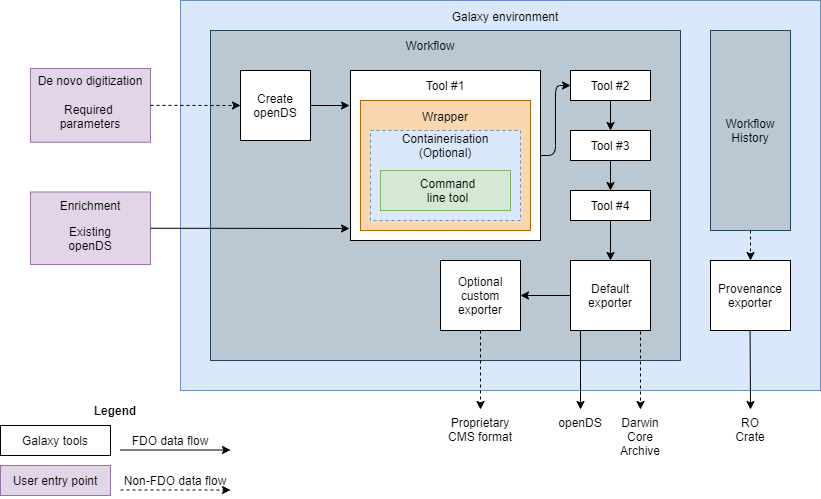
\includegraphics[width=\textwidth]{figures/ch08/figure2.png}
	\caption[CWFR approach]{\textbf{CWFR approach}. Adopted for the SDR as a Galaxy 
  workflow management system
  implementation with `\emph{de novo} digitization' and `enrichment' entry points.}
  \label{ch8:figure2}
\end{figure}


RO-Crate FDOs capture two aspects of a workflow:

\begin{enumerate}
\item
  A \textbf{Workflow-RO-Crate} contains the workflow definition, the
  computational tools and configuration, graphical image of the
  workflow, etc; this is the \emph{method} registered in the WorkflowHub
  and activated in the Specimen Data Refinery for execution.
\item
  A \textbf{Workflow-Run-RO-Crate} references (a) and records the
  details of a specific computational workflow run and its runtime
  information, with relations to the used and generated FDOs. This
  captures the digitization provenance that is generated as the openDS
  FDO makes its journey through a workflow.
\end{enumerate}

The final step in SDR workflows can be a data exporter tool, allowing
users to export the entire openDS object as is, or to convert and export
it in another format, such as CSV, DarwinCore Archive, etc. This
reconfigurable nature of data export allows users to define their own
transformer function to allow export to match formats specific to
specific collection management systems in use by their institution, such
that refined data can be repatriated. The provenance exporter transforms
Galaxy workflow history data into a Workflow-Run-RO-Crate FDO.

All FDO types are serialized as JSON.

\subsubsection{Canonical components}\label{canonical-components}

Each workflow component from a canonical library (to be built,
illustrated as tools \#1 - \#4 in figure \ref{ch8:figure2}) describes what attributes it
requires from the openDS FDO to be able to function, and the attributes
it will in turn populate or enrich. The interface between the component
and the openDS FDO is formed by the wrapper (orange in figure \ref{ch8:figure2}) around
the (optionally) containerized command-line tool (blue/green in figure
2). Canonical components can be used individually, or in series. The
openDS FDO data flows between components will always be of the same
type, being modified as the workflow proceeds.

This allows tools to function both as standalone components and as part
of any sequence of chained tools, provided that the specific openDS FDO
attributes required for a tool to work are pre-populated. This keeps the
SDR flexible and customisable for different digitization pipelines.

Two entry points are provided for users of the SDR. One is named as the
`\emph{de novo} digitization' entry point (figure \ref{ch8:figure2}) fulfilling the
needs of user story (2) where specimens are being newly digitized for
the first time. The second entry point, named as the `enrichment' entry
point (figure \ref{ch8:figure2}) fulfils the needs of user story (3) where an existing
openDS FDO (or reference to it) can be provided to the SDR as part of
the input data.

In parallel to manipulating openDS FDOs, the Refinery gathers the
minimum inputs and workflow components required to produce deterministic
output and produces a Workflow-Run-RO-Crate FDO.

\subsection{Experiments and analysis}\label{experiments-and-analysis}

\subsubsection{Experimental workflows}\label{experimental-workflows}

The workflows of the SDR compose different functional components
according to specific need: image segmentation, barcode reading, optical
character recognition, text contextualisation/entity recognition,
geocoding, taxonomic linkage, people linkage, specimen condition
checking, automated identification, and data export/conversion. Broadly
speaking there are two main kinds of workflow: (i) specimen workflows,
where the specimen itself is analysed for morphological traits, colour
analysis, condition checking and automated identification; and (ii) text
and label workflows, where handwritten, typed or printed text from the
image is read, named entities are classified, then linked to identifiers
or enhanced through post processing.

Both kinds of workflow can begin with initial openDS object creation
based on the submission of specimen image files and accompanying input
parameters through a forms-based user interface (\emph{de novo}
digitization entry point); or, alternatively, a pre-existing openDS
object with accompanying image object(s)can be supplied as the input
(enrichment entry point). Both kinds of workflow also rely on the image
segmentation component as the precursor for subsequent workflow steps.
Similarly, and if needed both kinds might use a format conversion and
export component as their final step; for example, if an openDS FDO is
not a natively compatible output for the next consuming application.

Although not within the scope of the present proof-of-concept, other
more precise workflows for enhancing specific aspects of existing
records can be foreseen. There are many specimen records, for example
where locality text, although digitally available, is not yet geocoded.
There are records with unlinked or ambiguous collector names that could
be linked/disambiguated; and records where unknown specimens still need
identifying.

\subsubsection{Experimental data and evaluation}\label{experimental-data-and-evaluation}

\paragraph{Evaluation images datasets}\label{evaluation-images-datasets}

The Refinery will be evaluated using sets of images, each composed of at
least 1,000 unique specimens for each of the three categories of
preserved specimen types: herbarium sheets, microscope slides and pinned
insects. For herbarium sheet images we will reuse an existing benchmark
dataset of 1,800 herbarium specimen images with corresponding
transcribed data \cite{ch8-59}. For microscope slide and pinned insect
specimen images similar evaluation datasets will be prepared against the
same label characteristics: written in different languages; printed or
handwritten; covering a wide range of dates; both type specimens and
general collections and will provide specimens from different families
and different parts of the world. Each test dataset set will be composed
of images from different institutions to ensure representation of
heterogeneity. For the present proof of concept, we limit the scope to
Latin alphabet languages. These datasets will also be used to train
Refinery models for use in tools (e.g., segmentation, named entity
recognition, object/feature detection). All the datasets will be made
publicly available with documentation.

\paragraph{Component functional tests}\label{component-functional-tests}

Galaxy has a built-in functional test framework. Tools intended to
become components of an SDR canonical library (actually, a Galaxy
ToolShed repository) will need to pass previously defined tests within
this framework. These tests, based on pre-supplied openDS FDO input and
output files containing the properties expected to be populated by the
tool, include validating a tool's own openDS FDO outputs by comparison
against the expected output file. It will be necessary to register
openDS FDOs as Galaxy custom data types.

\subsection{Results}\label{results}

openDS FDOs are the core data object at the heart of the SDR, playing
not only the workflow input/output role but acting also as a common data
structure between tool steps within the workflow. Users can launch the
workflow with either an openDS object, for further augmentation by the
SDR, or they can complete a form with the specimen information, which is
then converted to an openDS object before the workflow proper begins.

Each SDR Galaxy tool defines the properties it requires in JSONPath
syntax \cite{ch8-60}. The wrapper validates that these properties exist in
the openDS object, plucks them from the openDS JSON, makes them
available as named parameters, and passes these through to the tool
processing (via either a Docker or Python command line). The wrapper
validates the input openDS against the openDS schema, the tool performs
its processing and updates the openDS, and the wrapper validates the
changed openDS against the schema before writing to disk. For the
prototypical SDR, a static, local version of the openDS schema is used.
Future iterations will use referenceable versions of the openDS schema,
allowing for schema changes and for tools to validate their data input
and outputs against versions of the schema.

On ingestion, every openDS is assigned a persistent identifier, ensuring
unambiguity and referential integrity for every processed object. In
production, DOIs will be minted by the DiSSCo service; for the
proof-of-concept Handles with prefix \texttt{20.5000.1025/} will be
used.

\subsection{Discussion}\label{ch8:discussion}

\subsubsection{What is being achieved?}\label{ch8:what-is-being-achieved}

The design of the Specimen Data Refinery uses two kinds of FAIR Digital
Object -- openDS FDOs and RO-Crate FDOs. Each plays a role to ensure
`FAIRer' automated digitization for natural history specimens and
associated provenance capture:

\begin{itemize}
\item
  openDS FDOs act both as the input/output interface of a workflow and
  as the common intermediary pattern (canonical state) between steps
  within a workflow. They comply with DiSSCo data management principles
  and needs as outlined in the DiSSCo Data Management Plan \cite{ch8-28}
  allowing specimen data to be processed and extended in a fully FAIR
  manner \cite{ch8-6}.
\item
  RO-Crate FDOs record both the workflow definition and information
  about its configuration (shared as a method object) together with the
  details and context of the work done during a workflow run; details
  that are captured proprietarily within the adopted Galaxy environment
  and transformed to a common pattern (as another kind of canonical
  state) of provenance for later scrutiny and reproducibility of the
  work. These kinds of Research Objects \cite{Bechhofer 2013} are an established
  mechanism whereby computational methods become first-class citizens
  alongside data, to be easily shared, discussed, reused and repurposed
  \cite{ch8-57}.
\end{itemize}

Both kinds of FDO are essential. They complement one another to support
implementation of the FAIR principles, especially the interoperable and
reusable principles by making workflows self-documenting. This renders
automated whole processes (or fragments thereof) for digitizing and
extending natural history specimens' data as FAIR without adding
additional load to the researchers that stand to benefit most from that
\cite{ch8-27}. Each FDO type originates from different Research
Infrastructures (ELIXIR, DiSSCo) with different implementation
frameworks. Yet, they interoperate effectively due to their clear roles,
common conceptual model and separation of concerns.

\subsubsection{Different FDO implementations working together}\label{ch8:different-fdo-implementations-working-together}

openDS FDOs have their heritage in distributed digital object services
\cite{Kahn 2006} and are implemented through Digital Object Architecture (DOA)
\cite{ch8-62} with Digital Object Interface Protocol (DOIP) \cite{DONA 2018}, Digital
Object Identifier Resolution Protocol (DO-IRP) \cite{rfc3652}, and
recommendations of the Research Data Alliance \cite{ch8-65}. Serialized as
JSON, they are machine-actionable and compatible with established
protocols of the World Wide Web.

RO-Crates are native to the World Wide Web, based on established web
protocols, machine-readable metadata using Linked Data Platform methods
\cite{ch8-66}, JSON-LD and Schema.org \cite{Bechhofer 2013}, and community-accepted
packaging mechanisms such as BagIt. This makes RO-Crates straightforward
to incorporate into pre-existing platforms such as Galaxy and data
repositories such as Zenodo and DataVerse.

Both kinds of FDO use Persistent identifiers (PID), allowing instances
to be both uniquely identified and their location to be determined;
RO-Crates, as web natives, use URIs whereas openDS, as DOA objects, use
Handle PIDs. Instances of both kinds are described by metadata and
contain or reference data.

RO-Crates are self-describing using a metadata file and use
openly-extensible profiles to type the Crates (profile-typing) to set
out expectations for their metadata and content. openDS uses an
object-oriented object typing and instance approach to define the
structure and content of data/metadata. Complex object types are
constructed from basic types, an extension-section basic type. Both
approaches seek to avoid locking objects into repository silos, ensuring
that FDO instances can be interpreted outside of the contexts in which
they were originally created/stored.

Structurally and semantically openDS FDOs and RO-Crate FDOs are
potentially isomorphic, although at different granularity levels. Their
main difference is in method calling. As a DOA object, openDS would
expect to respond to type-specific method calls if these were
implemented. RO-Crates delegate actionability to applications that
interpret their self-describing profile.

Within the SDR the two kinds of FDO fulfill distinct and interlocking
roles for data (openDS) and self-documented method (RO-Crate) so their
different forms is not an issue. In future there may be a need to map
and convert between the approaches (e.g., for reconstructing past
processing), which would be assisted by the common FDO conceptual model
\cite{bonino2019}.

\subsubsection{Key domain challenges ahead}\label{key-domain-challenges-ahead}

For a digitized specimen to conform to FAIR principles, its data must be
linked to a vocabulary of terms, but choosing a single vocabulary is
likely to cause interoperability issues when cross-linking to resources
using another vocabulary, for example Darwin Core, Schema.org, or Access
to Biological Collection Data (ABCD). Whilst concepts can be mapped
across vocabularies (for example, using Simple Knowledge Organization
System (SKOS) matching), such an effort might rapidly become overly
complex and cumbersome, as the challenge of the Unified Medical Language
System (UMLS) demonstrates. The challenge remains - how is such a
mapping exercise maintained at a `just enough' level?

Different Earth Science domains have different use cases for digital
records. A digital record produced for biodiversity research is likely
to have different granularity, understanding and focus to one produced
for climate science. It remains to be seen if a single FAIR Digital
Object definition could be produced to satisfy multiple domains, and if
different objects could be produced for different domains, what would
they look like; and would this hinder future cross-compatibility?

The openDS FDO type produced by the SDR is a new object format for the
natural history domain that is foreseen to become an adopted standard
over time. Institutional collection management systems will need to be
upgraded before they can consume the FDO outputs from the SDR. Early
adopters may need assistance to produce SDR exporters matching
proprietary ingestion formats. For an interim period, there may be a
need for the SDR to output today's widely used Darwin Core Archives
format in parallel.

As the functional requirements of the SDR are emergent, a minimum viable
product has been scoped, but this should be contrasted with the notion
of a useful product. An MVP is a prototype; a tool to get a project off
the ground with enough features to be usable by early adopters, and to
build on to learn user requirements. But it is not intended to meet the
day-to-day requirements of all users. To nurture future development,
care must be taken to continue involving key stakeholders in eliciting
further requirements to make the SDR useful for the widest range of
users, and from there, develop a rich, configurable tool to allow simple
uptake and provide utility for resource-poor collections.

\subsection{Conclusion and Future Work}\label{conclusion-and-future-work}

The Specimen Data Refinery is likely to garner widespread interest
across the Natural History community. Whilst the promise of a scalable,
community-driven digitization platform is tantalising for many natural
history professionals, the Specimen Data Refinery project is still in
its early stages, and, as discussed above key challenges lie ahead.

Although natural history collections are generally catalogued by the
taxonomic identity of the curated object, there remains a large
historical backlog of unidentified specimens. The Meise Botanic Garden
(BE), for example, has an estimated 4 million specimens with at least
11\% not yet identified to species level. Furthermore, it is calculated
that half of the World's estimated 70,000 plant species yet to be
described have already been collected and are waiting in collections
still to be `discovered' \cite{Crusoe 2022}. The same is likely to be true for
other groups of organisms, especially insects. Unnamed specimens tend to
have lowest priority for digitization and their data are rarely shared.
Machine learning as canonical steps in SDR workflows presents a
tremendous opportunity to put an identification on these specimens and
potentially, to triage them for further taxonomic investigation.



\section[Incrementally building FAIR Digital Objects with the Specimen Data Refinery]{Incrementally building FAIR Digital Objects with Specimen Data Refinery workflows}
\label{ch7:incrementally-building-fair-digital-objects-with-specimen-data-refinery-workflows}

\emph{Specimen Data Refinery} (\acrshort{SDR}) is a developing platform for
automating transcription of specimens from natural history collections
\cite{Hardisty 2022} (section \vref{ch8:the-specimen-data-refinery}). SDR is
based on computational workflows and digital twins using
\acrlongpl{FDO}.
%FAIR Digital Objects.

We show our recent experiences with building SDR using the Galaxy
workflow system and combining two FDO methodologies with open digital
specimens (\acrshort{openDS}) and RO-Crate data packaging. We suggest FDO
improvements for incremental building of digital objects in
computational workflows.

\subsection{SDR workflows}\label{ch7:sdr-workflows}

\footurl{https://sdr.nhm.ac.uk/}{SDR} is realised as the workflow system
Galaxy \cite{Afgan 2018} with
\footurl{https://github.com/DiSSCo/SDR}{SDR tools} installed. An Open
Research challenge is that some tools have machine learning models with
a commercial licence. This complicates publishing to
\footurl{https://toolshed.g2.bx.psu.edu/}{Galaxy toolshed} -- however, we
created \footurl{https://www.ansible.com/}{Ansible} scripts to install
equivalent Galaxy servers, including tools and dependencies, accounts
and workflows. SDR workflows are
\footurl{https://workflowhub.eu/projects/72}{published in WorkflowHub} as
FDOs.

We implemented the use case \emph{De novo digitization} in Galaxy \cite{Brack 2022b}.
Shown in Figure \vref{ch7:figure1} the
workflow steps exchange openDS \acrshort{JSON} \cite{Hardisty 2019a}, for
incremental completion of a digital specimen. Initial stages build a
template openDS from a \acrshort{CSV} with metadata and image references --
subsequent analysis completes the rest of the JSON with \emph{regions}
of interest, \emph{text} digitised from handwriting, and recognised
\emph{named entities}.

\begin{figure}%[t]
    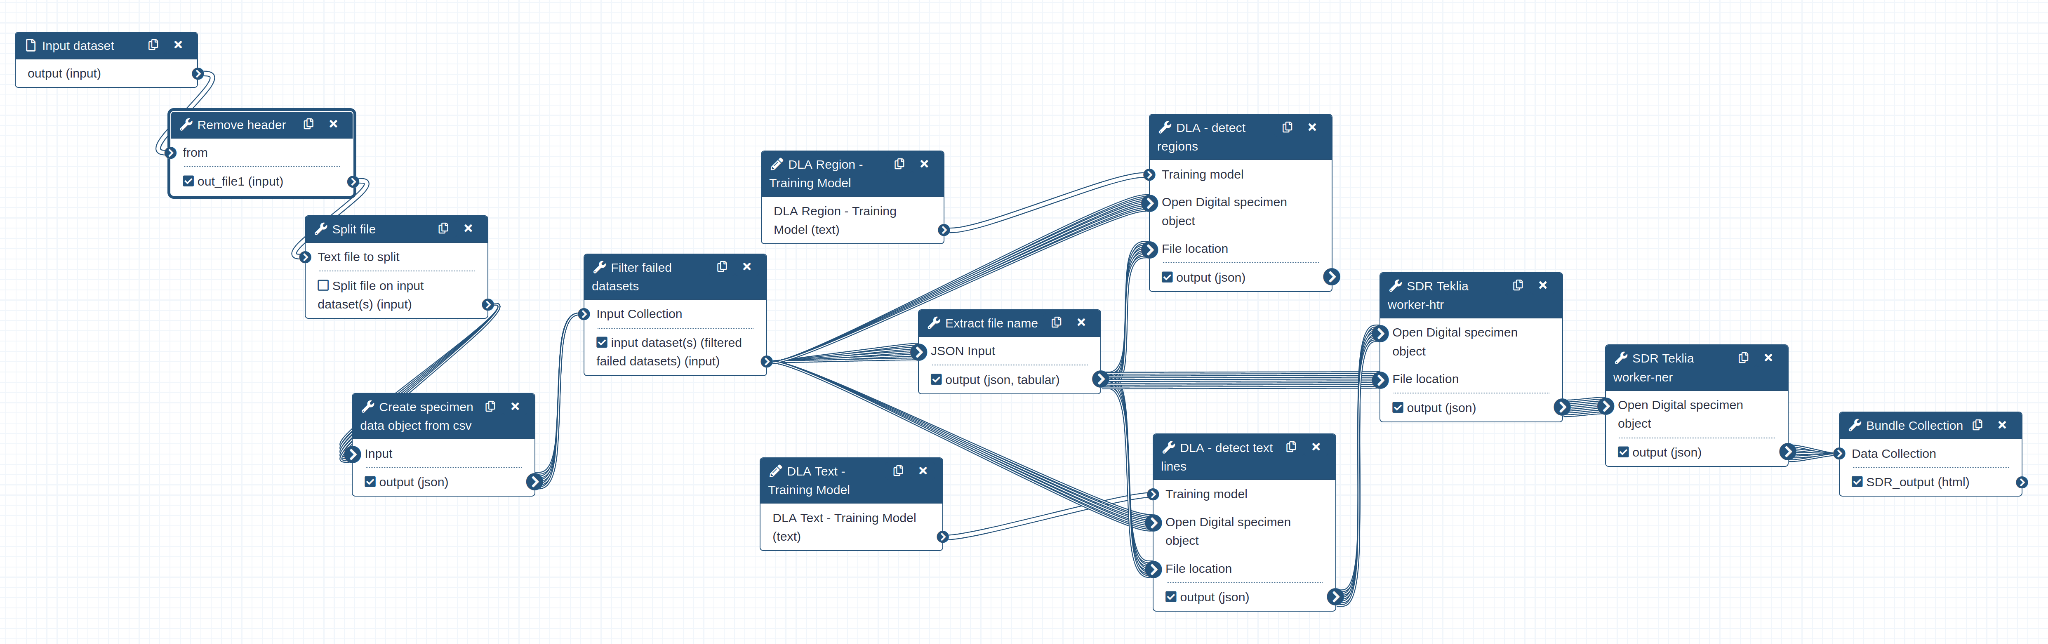
\includegraphics[width=\textwidth]{figures/ch07/figure1.png}
	\caption[FDO propagation in workflow]{\textbf{FDO propagation in workflow}. 
    Draft Galaxy workflow \cite{Brack 2022b} 
    shows propagation of partial Open Digital Specimen FDOs between
    individual canonical workflow building blocks. First steps process a \acrshort{CSV}
    file to create the initial openDS, where referenced images are analysed
    to detect text lines which are \acrshort{OCR}ed and then recognised as named
    entities. Bands indicate flow of collections of openDS, processed
    concurrently by each step. The final step bundles the collection of
    openDS FDOs as JSON files in a \gls{ZIP} archive.}
    \label{ch7:figure1}
  \end{figure}

Galaxy can visualise outputs of each step
(Figure \vref{ch7:figure2}), important to make the
FDOs understandable by domain experts and to verify accuracy of SDR.

\begin{figure}%[t]
    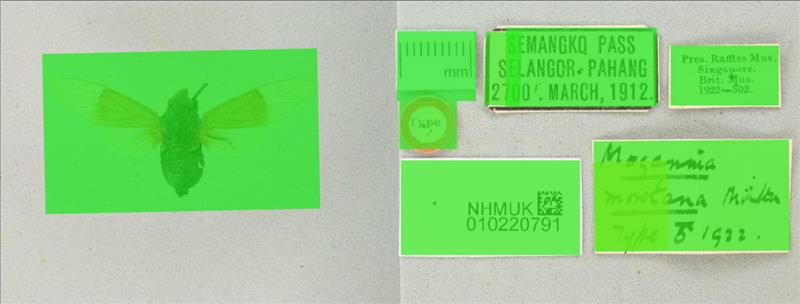
\includegraphics[width=\textwidth]{figures/ch07/figure2.jpg}
	\caption[Visualising openDS FDO within Galaxy]{\textbf{Visualising openDS FDO within Galaxy}.
    Showing detected regions of interest
    (specimen, labels and scale bar) for a pinned insect.}
    \label{ch7:figure2}
\end{figure}

We are adding workflows for partial stages, e.g.~detection of regions
\cite{Livermore 2022a} and hand-written text recognition
\cite{Livermore 2022b}, which we will combine with scalability testing and wider
testing by project users. Additional workflows will enhance existing
FDOs and use new tools such as barcode detection of museums' internal
identifiers.

We are now ready to publish digital specimens as FAIR Digital Objects,
with registration into \footurl{https://www.dissco.eu/dissco/technical-infrastructure/}{DiSSCO repositories}, PID assignment and workflow provenance. However, even at
this early stage we have identified several challenges that need to be
addressed.

\subsection{FDO lessons}\label{ch7:fdo-lessons}

We highlight the \emph{de novo} use case because this workflow is
exchanging \emph{partial} FDOs -- openDS objects which are not fully
completed and not yet assigned persistent identifiers.
\footurl{https://github.com/DiSSCo/openDS}{openDS schemas} are still in
development, therefore SDR uses a
more flexible
\footurl{https://github.com/DiSSCo/SDR/blob/main/galaxy-workflow/config/opends-schema.json}{JSON schema} where only the initial metadata (populated from CSV) are
required. Each step validates the partial FDO before passing it to the
underlying command line tool.

Although workflow steps exchange openDS objects, they cannot be combined
in any order. For instance, \emph{named entity recognition} requires
digitised text in the FDO. We can consider these intermediate steps as
\emph{sub-profiles} of an FDO Type. Unlike hierarchical subclasses,
these FDO profiles are more like
\footurl{https://en.wikipedia.org/wiki/Duck_typing}{ducktyping}. For
instance a \emph{text detection} step may only require the
\texttt{regions} key, but semantically there is no requirement for say
\texttt{OpenDSWithText} to be a subclass of \texttt{OpenDSWithRegion},
as text also can be transcribed manually without regions.

Similarly, we found that some steps can be executed in parallel, but
this requires merging of partial FDOs. This can be achieved by combining
JSON queries and JSON Schemas, but indicates that it may be more
beneficial to have FDO fragments as separate objects. Adding openDS
fragment steps would, however, complicate workflows.

Several of our tools process the referenced images, currently \texttt{https} URLs
in openDS. We added a caching layer to avoid repeated image downloading,
coupled with local file-paths wiring in the workflow. A similar
challenge occurs if accessing image data using DOIP, which unlike HTTP,
has no caching mechanisms.

\subsection{RO-Crate lessons}\label{ch7:ro-crate-lessons}

Galaxy is developing\footnote{
    Completed after publication of this article, see section \vref{ch54:galaxy}.
} support for importing and
exporting Workflow
Run Crates\footnote{\url{https://www.researchobject.org/workflow-run-crate/} see also section \vref{ch54:wrroc}.}, a profile of RO-Crate \cite{Soiland-Reyes 2022a} to
captures execution history of a workflow, including its definition and
intermediate data \cite{De Geest 2022}. SDR is adopting this support to
combine openDS FDOs with workflow provenance, as envisioned by
\cite{Walton 2020a}.

Our prototype \emph{de novo} workflow returns results as a ZIP file of
openDS objects. End-users should also get copies of the referenced
images and generated visualisations, along with workflow execution
metadata. We are investigating ways to embed the preliminary Galaxy
workflow history before the final step, so that this result can be an
enriched RO-Crate.

\subsection{Conclusions}\label{ch7:conclusions}

SDR is an example of machine-assisted construction of FDOs, which
highlight the needs for intermediate digital objects that are not yet
FDO compliant. The passing of such ``local FDOs'' is beneficial not just
for efficiency and visual inspection, but also to simplify workflow
composition of canonical workflow building blocks. At the same time we
see that it is insufficient to only pass FDOs as JSON objects, as they
also have references to other data such as images, which should not need
to be re-downloaded.

Further work will investigate the use of RO-Crate as a wrapper of
partial FDOs, but this needs to be coupled with more flexible FDO types
as profiles, in order to restrict ``impossible'' ordering of steps
depending on particular inner FDO fragments. A distinction needs to be
made between open digital specimens that are in ``draft'' state and
those that can be pushed to DiSSCo registries.

We are experimenting with changing the SDR components into Canonical
Workflow Building Blocks \cite{Soiland-Reyes 2022b}
(section \vref{ch6:making-canonical-workflow-building-blocks-interoperable-across-workflow-languages}) 
using the Common Workflow Language \cite{Crusoe 2022}. This gives
flexibility to scalably execute SDR workflows on different compute
backends such as HPC or local cluster, without the additional setup of
Galaxy servers.


\section{Recording provenance of workflow runs with RO-Crate}
\label{ch54:wrroc}

Recording the provenance of scientific computation results is key to the support of traceability, reproducibility and quality assessment of data products.
Several data models have been explored to address this need, providing representations of workflow plans and their executions as well as means of packaging the resulting information for archiving and sharing.
However, existing approaches tend to lack interoperable adoption across workflow management systems.
In this work we present Workflow Run RO-Crate, an extension of RO-Crate (Research Object Crate) and Schema.org to capture the provenance of the execution of computational workflows at different levels of granularity and bundle together all their associated products (inputs, outputs, code, etc.).
The model is supported by a diverse, open community that runs regular meetings, discussing development, maintenance and adoption aspects.
Workflow Run RO-Crate is already implemented by several workflow management systems, allowing interoperable comparisons between workflow runs from heterogeneous systems.
We describe the model, its alignment to standards such as W3C PROV, and its implementation in six workflow systems.
Finally, we illustrate the application of Workflow Run RO-Crate in two use cases of machine learning in the digital image analysis domain.



\subsection{Introduction}\label{ch54:introduction}

A crucial part of scientific research is recording the provenance of its outputs.
The W3C PROV standard defines provenance as ``a record that describes the people, institutions, entities, and activities involved in producing, influencing, or delivering a piece of data or a thing''
\cite{Moreau 2013}.
Provenance is instrumental to activities such as traceability, reproducibility, accountability, and quality assessment
\cite{Herschel 2017}.
The constantly growing size and complexity of scientific datasets and the analysis that is required to extract useful information from them has made science increasingly dependent on advanced automated processing techniques in order to get from experimental data to final results~\cite{Himanen 2019, Gauthier 2019, Huntingford 2019}.
Consequently, a large part of the provenance information for scientific outputs consists of descriptions of complex computer-aided data processing steps. This data processing is often expressed as workflows, i.e., high-level applications that coordinate multiple tools and manage intermediate outputs in order to produce the final results.

In order to homogenise the collection and interchange of provenance records, the W3C consortium proposed the PROV-O standard~\cite{w3-prov-o}, an OWL \cite{w3-owl2-overview} representation of PROV for provenance in the Web.
PROV-O has been widely extended for workflows (D-PROV \cite{Missier 2013}, ProvONE \cite{Cuevas-Vicenttín 2016}, OPMW \cite{Garijo 2011}, P-PLAN \cite{Garijo 2012}), where provenance information is collected in two main forms: prospective and retrospective~\cite{Freire 2008}. \emph{Prospective provenance} -- the execution plan -- is essentially the workflow itself: it includes a machine-readable specification with the processing steps to be performed and the data and software dependencies to carry out each computation.
\emph{Retrospective provenance} refers to what actually happened during an execution, i.e.~what were the values of the input parameters, which outputs were produced, which tools were executed, how much time did the execution take, whether the execution was successful or not, etc.
Retrospective provenance can also be represented at different levels of abstraction depending on available computing resources: for instance, by the workflow execution becoming a single activity which produces results, by specifying the individual execution of each workflow step, or by going a step further and indicating how each step is divided into sub-processes when a workflow is deployed in a cluster.

Different workflow systems have adopted and extended PROV (and its PROV-O representation) to the workflow domain (Pegasus \cite{Deelman 2005}, WINGS \cite{Gil 2011, Garijo 2014}, VisTrails \cite{Scheidegger 2008,Costa 2013}), in order to ease the burden of provenance collection from tool developers to workflow management systems (WMS) \cite{Atkinson 2017,Pérez 2018}.

D-PROV, PROV-ONE, OPMW-PROV, P-Plan propose representations of workflow plans and their respective executions, taking into account the features of the workflow systems implementing them (e.g., hierarchical representations, sub-processes, etc.).
Other data models like \emph{wfprov} and \emph{wfdesc}
\cite{Belhajjame 2015} go a step further by considering not only the link between plans and executions, but how to package the various artefacts as a Research Object (RO) ~\cite{Bechhofer 2013} in order to ease portability while keeping the context of a digital experiment.

However, while these models address some workflow provenance representation issues, they have two main limitations: firstly, the extensions of PROV are not directly interoperable because of differences in granularity or different assumptions in their workflow representations; secondly, their support from WMS is typically one system per model.  An early approach to unify and integrate workflow provenance traces across WMS was WEST (Workflow Ecosystems through STandards) \cite{Garijo 2014}, through the use of WINGS \cite{Gil 2011} to build workflow templates and different converters. In all of these workflow provenance models, the emphasis is on the workflow execution structure as a directed graph, with only partial references for the data items. 

More recently, interoperability have been partially addressed by Common Worlflow Language Prov (CWLProv)~\cite{Khan 2019}, which represents workflow enactments as ROs serialised according to the Big Dta Bag (BDBag) approach~\cite{Chard 2016}.
The resulting format is a folder containing several data and metadata files~\cite{Soiland-Reyes 2018}, expanding on the RO Bundle approach of Taverna \cite{Soiland-Reyes 2016}.
CWLProv also extends PROV with a representation of executed processes (activities), their inputs and outputs (entities) and their executors (agents), together with their Common Workflow Language specification
\cite{Crusoe 2022} -- a standard workflow specification adopted by at least a dozen different \footurl{https://www.commonwl.org/implementations/}{workflow systems}. Although CWLProv includes prospective provenance as a \emph{plan}
within PROV (based on the \emph{wfdesc} model), in practice its implementation does not include tool definitions or file formats, as proposed by the wfdesc extension \footurl{https://wf4ever.github.io/ro/2016-01-28/roterms}{Roterms}.
In order for CWLProv consumers to reconstruct the full prospective provenance for understanding the workflow, they would also need to inspect the separate workflow definition in the native language of the WMS.
Additionally, the CWLProv RO may include several other metadata files and PROV serialisations conforming to different formats, complicating its generation and consumption.

As for granularity, CWLProv proposed multiple levels of provenance \cite[figure 2]{Khan 2019}, from Level 0 (capturing workflow definition) to Level 3 (domain-specific annotations). 
In practice, the CWL reference implementation \emph{cwltool} \cite{Amstutz 2023} and the corresponding CWLProv specification \cite{Soiland-Reyes 2018} records provenance details of all task executions together with the intermediate data and any nested workflows (CWLProv level 2), a granularity level that requires substantial support from the WMS
\cite{Soiland-Reyes 2022}.
This approach is appropriate for workflow languages where the execution plan, including its distribution among the various tasks, is well known in advance (such as CWL).
However, it can be at odds with other systems where the execution is more dynamic, depending on the verification of specific runtime conditions, such as the size and distribution of the data (e.g., COMPSs~\cite{Lordan 2014}).
This makes the implementation of CWLProv challenging, as shown by the fact that at the time of writing the format is supported only by cwltool.
Finally, being based on the PROV model, CWLProv is highly focused on the interaction between agents, processes and related entities, while support for contextual metadata (such as workflow authors, licence or creation date) in the Research Object Bundle is \footurl{https://w3id.org/bundle/context}{limited} and stored in a separate manifest file, that includes the data identifier mapping to filenames.
A project that uses serialised ROs similar to those used by CWLProv is Whole Tale \cite{Chard 2019}, a web platform with a focus on the narrative around scientific studies and their reproducibility, where the serialised ROs are used to export data and metadata from the platform. In contrast, our work is primarily focused on the ability to capture the provenance of computational workflow execution including its data and executable workflow definitions.

RO-Crate~\cite{Soiland-Reyes 2022} is a recent approach to packaging research data together with their metadata; it extends Schema.org~\cite{Guha 2015}, a popular vocabulary for describing resources on the Web.
In its simplest form, an RO-Crate is a directory structure that contains a single JSON-LD \cite{w3-json-ld} metadata file at the top level.
The metadata file describes all entities stored in the RO-Crate along with their relationships; it is both machine-readable and human-readable.
RO-Crate is general enough to be able to describe any dataset, but can also be made as specific as needed through the use of extensions called
\emph{profiles}.
At the same time, the broad set of types and properties from Schema.org, complemented by a few additional terms from other vocabularies, make the RO-Crate model capable of expressing a wide range of contextual information that complements and enriches the core information specified by the profile.
This may include, among others, the workflow authors and their affiliations, associated publications, licensing information, related software, etc.
This is an approach used by WorkflowHub \cite{Goble 2021}, a workflow system agnostic workflow registry which specifies a Workflow RO-Crate profile \cite{Bacall 2022} to gather the workflow definition with such metadata in an archived RO-Crate. 

In this work, we present \textbf{Workflow Run RO-Crate} (WRROC), an extension of RO-Crate for representing computational workflow execution provenance.
Our main contributions are the following:

\begin{itemize}
\item   A collection of RO-Crate profiles to represent both the prospective and the retrospective provenance of a computational workflow run in a way that is machine-actionable \cite{Batista 2022}, independent of the specific  workflow language or execution system, and including support for rerunnability.
\item   Implementations of the model in six workflow systems, and a mapping against the W3C PROV-O Standard
\item   A governance model, held by an open community (Workflow Run RO-Crate) to discuss extensions,  issues and new implementations for the proposed profiles.
\end{itemize}

To foster usability, the profiles are characterised by different levels of detail, and the set of mandatory metadata items is kept to a minimum in order to ease the implementation.
This flexible approach increases the model's adaptability to the diverse landscape of WMS used in practice.
The base profile, in particular, is applicable to any kind of computational process, not necessarily described in a formal workflow language.
In this work we describe seven implementations (six in WMS and one in a conversion tool) and demonstrate the application of the profiles to multiple use cases.

The rest of this section is organised as follows: we first describe the Workflow Run RO-Crate profiles; we then illustrate implementations and usage examples; this is followed by a discussion and plans for future work.


%% 
\subsection{The Workflow Run RO-Crate profiles}\label{ch54:the-workflow-run-ro-crate-profiles}

RO-Crate profiles are extensions of the base RO-Crate specification that describe how to represent the entities and relationships that appear in a specific domain or use case.
An RO-Crate conforming to a profile is not just machine-readable, but also machine-actionable as a digital object whose type is represented by the profile itself~\cite{10.3897/rio.8.e93937}.

The Workflow Run RO-Crate profiles are the main outcome of the activities of the Workflow Run RO-Crate \footurl{https://www.researchobject.org/workflow-run-crate}{Community}, an open working group that includes workflow users and developers, WMS users and developers, and researchers and software engineers interested in workflow execution provenance and FAIR approaches for data and software.
In order to develop the Workflow-Run RO-Crate profiles, one of the first community efforts was to compile a list of requirements in the form of competency \footurl{https://www.researchobject.org/workflow-run-crate/requirements}{questions} to be addressed by the model.
Each requirement was backed up by a rationale and linked to a GitHub issue to drive the discussion forward. When a requirement was addressed, related changes were integrated into the profiles and the relevant issue was closed. Many of the original issues are now closed, and the profiles have had three official releases on Zenodo.


As requirements were being defined, it became apparent that one single profile would not have been sufficient to cater to all possible usage scenarios.
In particular, while some use cases required a detailed description of all computations orchestrated by the workflow, others were only concerned with a ``black box'' representation of the workflow and its execution as a whole.
Additionally, some computations involve a data flow across multiple applications that are executed without the aid of a WMS and thus are not formally described in a standard workflow language.
These observations led to the development of three profiles: 

\begin{enumerate}[(1)]
  \item \footurl{https://w3id.org/ro/wfrun/process/0.1}{Process Run Crate}
  \cite{WRROC 2023a} to describe the execution of one or more tools that contribute to a computation
  \item \footurl{https://w3id.org/ro/wfrun/workflow/0.1}{Workflow Run Crate}
  \cite{WRROC 2023b} to describe a computation orchestrated by a predefined workflow 
  \item \footurl{https://w3id.org/ro/wfrun/provenance/0.1}{Provenance Run Crate}
  \cite{WRROC 2023c} to describe a workflow computation including the internal details of individual step executions.
\end{enumerate}
  
In the rest of this section we describe each of the above profiles in detail.
We use italics to denote the types and properties used to describe entities and their relationships: these are defined in the RO-Crate JSON-LD \footurl{https://www.researchobject.org/ro-crate/1.1/context.jsonld}{context}, which extends Schema.org with terms from the Bioschemas \cite{Gray 2017} ComputationalWorkflow \footurl{https://bioschemas.org/profiles/ComputationalWorkflow/1.0-RELEASE}{profile} and other vocabularies. More specifically, from Bioschemas we use the \emph{ComputationalWorkflow} and \emph{FormalParameter} types as well as the \emph{input} and \emph{output} properties. 
Note that these terms, though coming from Bioschemas, are not specific to the life sciences.
We also developed a context extension through a dedicated ``workflow-run'' \footurl{https://w3id.org/ro/terms/workflow-run\#}{namespace} to represent concepts that are not captured by terms in the RO-Crate context.

\subsubsection{Process Run Crate}\label{ch54:process-run-crate}

The Process Run Crate profile contains guidelines on describing the execution of one or more software applications that contribute to the same overall computation, but are not necessarily coordinated by a top-level workflow or script.
For instance, they could be executed manually by a human agent, one after the other as intermediate datasets become available.

Being the basis for all profiles in the WRROC collection, Process Run Crate specifies how to describe the fundamental entities involved in a computational run: a software application (represented by a
\emph{SoftwareApplication}, \emph{SoftwareSourceCode} or
\emph{ComputationalWorkflow} entity) and its execution (represented by a \emph{CreateAction} entity), with the latter linking to the former via the \emph{instrument} property.
Other important properties of the
\emph{CreateAction} entity are \emph{object}, which links to the action's inputs, and \emph{result}, which links to its outputs.
The time the execution started and ended can be provided, respectively, via the
\emph{startTime} and \emph{endTime} properties.
The \emph{Person} or
\emph{Organization} entity that performed the action is referred to via the \emph{agent} property.
Fig~\vref{ch54:fig:process_crate_er} shows the entities used in Process Run Crate together with their relationships.

\begin{figure}[!ht]
  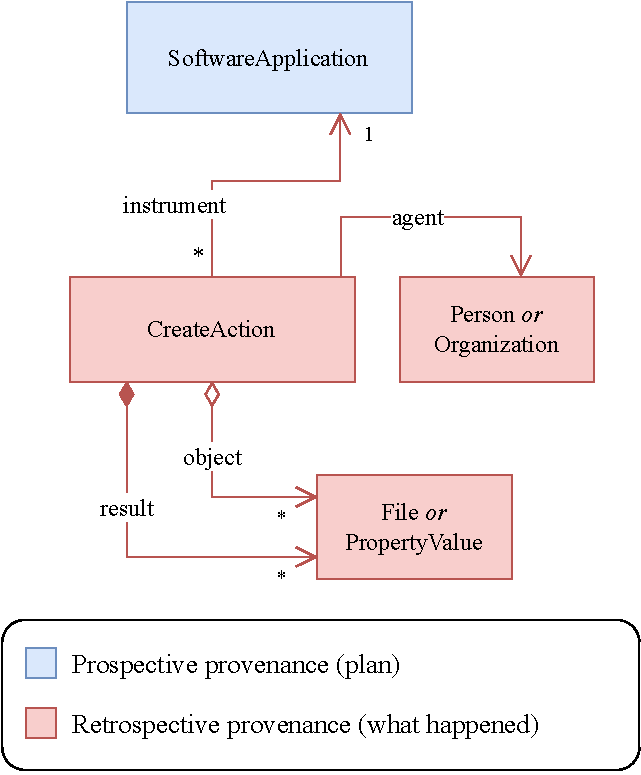
\includegraphics[width=26em]{figures/ch54/wrroc-figure1.drawio.pdf}
  \caption[UML class diagram for Process Run Crate]{{\bf UML class diagram for Process Run Crate.}
The central entity is the \emph{CreateAction}, which represents the execution of an application.
It relates with the application itself via \emph{instrument}, with the entity that executed it via \emph{agent} and with its inputs and outputs via \emph{object}
and \emph{result}, respectively. 
\emph{File} is an RO-Crate alias for Schema.org's \emph{MediaObject}.
Some inputs (and, less commonly, outputs), however, are not stored as files or directories, but passed to the application (e.g., via a command line interface) as values of various types (e.g., a number or string). In this case, the profile recommends a representation via \emph{PropertyValue}. 
For simplicity, we left out the rest of the RO-Crate structure (e.g. the root \emph{Dataset}). In this UML class notation diamond $\Diamond$ arrows indicate aggregation and regular arrows indicate references, $*$ indicates multiple instances, $1$ means single instance.  
}
\label{ch54:fig:process_crate_er}
\end{figure}

As an example,
suppose a user called John Doe runs the \texttt{head} UNIX command to extract the first ten lines of an input file called lines.txt, storing the result in another file called \texttt{selection.txt}.
Then, the same user runs the \texttt{sort}
command on \texttt{selection.txt}, storing the sorted output in a file called \texttt{sorted\_selection.txt}.
Fig~\vref{ch54:fig:head_sort} contains a diagram of the two actions and their relationships to the other entities involved.
Note how the actions are connected by the fact that the output of ``Run Head'' is also the input of ``Run Sort'': they form an ``implicit workflow'', whose steps have been executed manually rather than by a higher level software tool.


\begin{figure}[!ht]
  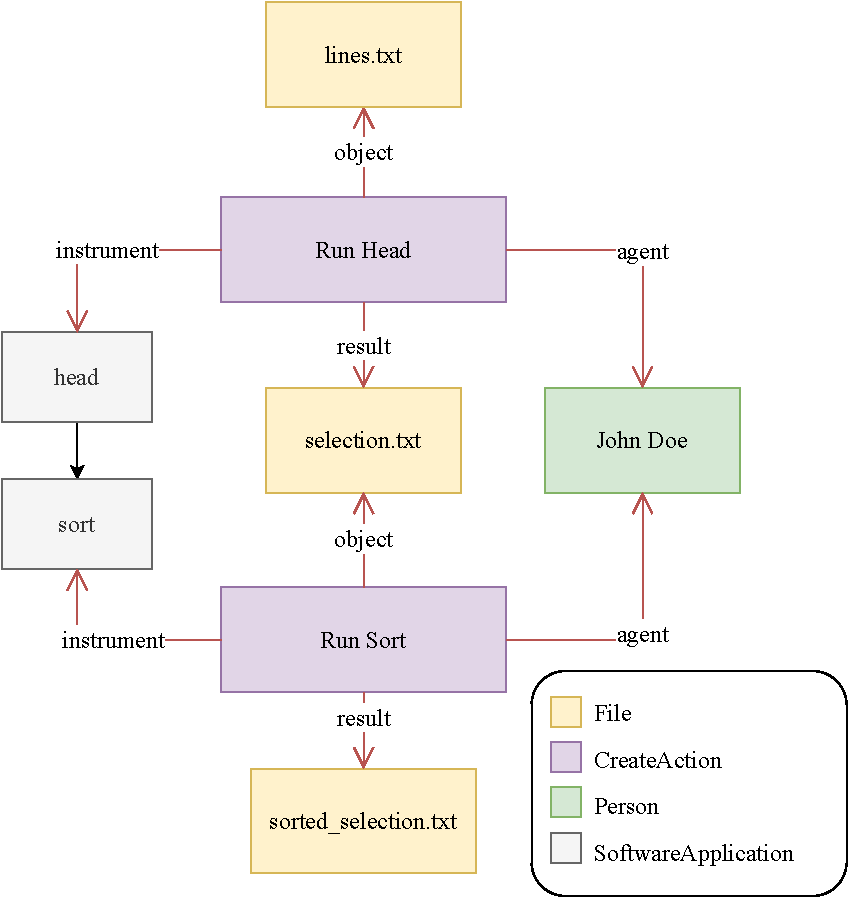
\includegraphics[width=29em]{figures/ch54/wrroc-figure-example.drawio.pdf}
\caption[Object diagram of a simple workflow]{{\bf Object diagram of a simple workflow} where the \texttt{head} and \texttt{sort} programs were run manually by a user.
The executions of the individual software programs are connected by the fact that the file output by \texttt{head} was used as input for \texttt{sort}, documenting the computational flow in an implicit way.
Such executions can be represented with Process Run Crate.}
\label{ch54:fig:head_sort}
\end{figure}


Process Run Crate extends the RO-Crate guidelines on representing software used to create files with additional requirements and conventions.
This arrangement is typical of the RO-Crate approach, where the base specification provides general recommendations to allow for high flexibility, while profiles -- being more concerned with the representation of specific domains and machine actionability -- provide more detailed and structured definitions.
Nevertheless, in order to be broadly applicable, profiles also need to avoid the specification of too many strict requirements, trying to strike a good trade-off between flexibility and actionability.
One of the implications of this approach is that consumers need to code defensively, avoiding unwarranted assumptions -- e.g. by verifying that a value exists for an optional property before trying to retrieve it and use it.


\subsubsection{Workflow Run Crate}\label{ch54:workflow-run-crate}

The Workflow Run Crate profile combines the Process Run Crate and WorkflowHub's Workflow RO-Crate \cite{Bacall 2022} profiles to describe the execution of “proper” computational workflows managed by a WMS.
Such workflows are typically written in a special-purpose language, such as CWL or Snakemake
\cite{Koster 2012}, and run by one or more WMS (e.g., StreamFlow
\cite{Colonnelli 2020}, Galaxy~\cite{Galaxy 2022}).
As in Process Run Crate, the execution is described by a \emph{CreateAction}
that links to the application via \emph{instrument}, but in this case the application must be a workflow, as prescribed by Workflow RO-Crate.
More specifically, Workflow RO-Crate states that the RO-Crate must contain a main workflow typed as \emph{File}, \emph{SoftwareSourceCode}
and \emph{ComputationalWorkflow}.
The execution of the individual workflow steps, instead, is not represented: that is left to the more detailed Provenance Run Crate profile (described in the next section).

The Workflow Run RO-Crate profile also contains recommendations on how to represent the workflow's input and output parameters, based on the aforementioned Bioschemas~\cite{Gray 2017} ComputationalWorkflow profile.
All these elements are represented via the \emph{FormalParameter} entity and are referenced from the main workflow via the \emph{input} and
\emph{output} properties.
While the entities referenced from
\emph{object} and \emph{result} in the \emph{CreateAction} represent data entities and argument values that were actually used in the workflow execution, the ones referenced from \emph{input} and
\emph{output} correspond to formal parameters, which acquire a value when the workflow is run (see Fig.~\vref{ch54:fig:workflow_crate_er}).
In the profile, the relationship between an actual value and the corresponding formal parameter is expressed through the \emph{exampleOfWork} property -- the downloadable file is a realisation of the formal parameter definition.
For instance:

\begin{verbatim}
{
    "@id": "#annotations",
    "@type": "FormalParameter",
    "additionalType": "File",
    "encodingFormat": "text/tab-separated-values",
    "valueRequired": "True",
    "name": "annotations"
},
{
    "@id": "final-annotations.tsv",
    "@type": "File",
    "contentSize": "14784",
    "exampleOfWork": {"@id": "#annotations"}
}
\end{verbatim}

The derivation of Workflow Run Crate from Workflow RO-Crate makes RO-Crates that conform to this profile compatible with the WorkflowHub workflow registry by also conforming to its Workflow RO-Crate profile.
Thus, users of a WMS that implements this profile (or Provenance Run Crate, which inherits it) are able to register their workflows in WorkflowHub -- together with an execution trace -- by simply running them and uploading the resulting RO-Crates.
Additionally, the inheritance mechanism allows to reuse the specifications already developed for Workflow RO-Crate, which form part of the guidelines on representing the prospective provenance.

Fig~\vref{ch54:fig:workflow_crate_er} shows the entities used in Workflow Run Crate together with their relationships.

\begin{figure}[!ht]
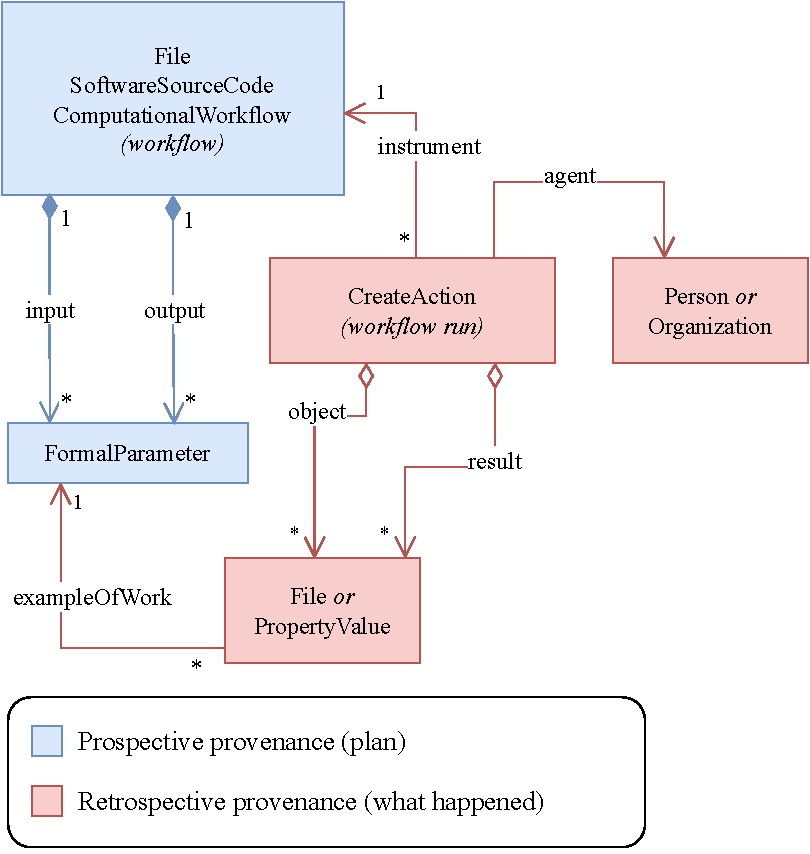
\includegraphics[width=26em]{figures/ch54/wrroc-figure2.drawio.pdf}
\caption[UML class diagram for Workflow Run Crate]{{\bf UML class diagram for Workflow Run Crate.}
The main differences with Process Run Crate are the representation of formal parameters and the fact that the application is expected to be an entity with types \emph{File}, \emph{SoftwareSourceCode} and \emph{ComputationalWorkflow}.
Effectively, the entity belongs to all three types, and its properties are the union of the properties of the individual types.
The filled diamond $\blacklozenge$ indicates composition, empty diamond $\Diamond$ aggregation, and other arrows relations.
}
\label{ch54:fig:workflow_crate_er}
\end{figure}


\subsubsection{Provenance Run Crate}\label{ch54:provenance-run-crate}

The Provenance Run Crate profile extends Workflow Run Crate by adding specifications on how to describe the internal details of the workflow run, including individual tool executions, intermediate outputs and related parameters.
Individual tool executions are represented by additional \emph{CreateAction} instances that refer to the tool itself via \emph{instrument} -- analogously to its use in Process Run Crate.
The workflow is required to refer to the tools it orchestrates through the \emph{hasPart} property, a specification also found in the Bioschemas ComputationalWorkflow profile, though in the latter it is only a recommendation.

To represent the logical steps defined by the workflow, this profile introduces the usage of \emph{HowToStep} i.e., “A step in the instructions for how to achieve a result”\footurl{https://schema.org/HowToStep}{}.
Steps point to the corresponding tools via the \emph{workExample} property and are referenced from the workflow via the \emph{step} property; the execution of a step is represented by a \emph{ControlAction} pointing to the
\emph{HowToStep} via \emph{instrument} and to the \emph{CreateAction}
instance(s) that represent the corresponding tool execution(s) via
\emph{object}.
Note that a step execution does not coincide with a tool execution: an example where this distinction is apparent is when a step maps to multiple executions of the same tool over a list of inputs (e.g. the ``scattering'' feature in CWL).

An RO-Crate following this profile can also represent the execution of the WMS itself (e.g., cwltool) via
\emph{OrganizeAction}, pointing to a representation of the WMS via
\emph{instrument}, to the steps via \emph{object} and to the workflow run via \emph{result}.
The \emph{object} attribute of the
\emph{OrganizeAction} can additionally point to a configuration file containing a description of the settings that affected the behaviour of the WMS during the execution.

Fig~\vref{ch54:fig:provenance_crate_er} shows the various entities involved in the representation of a workflow run via Provenance Run Crate together with their relationships.

\begin{figure}[ht]
  \begin{center}    
    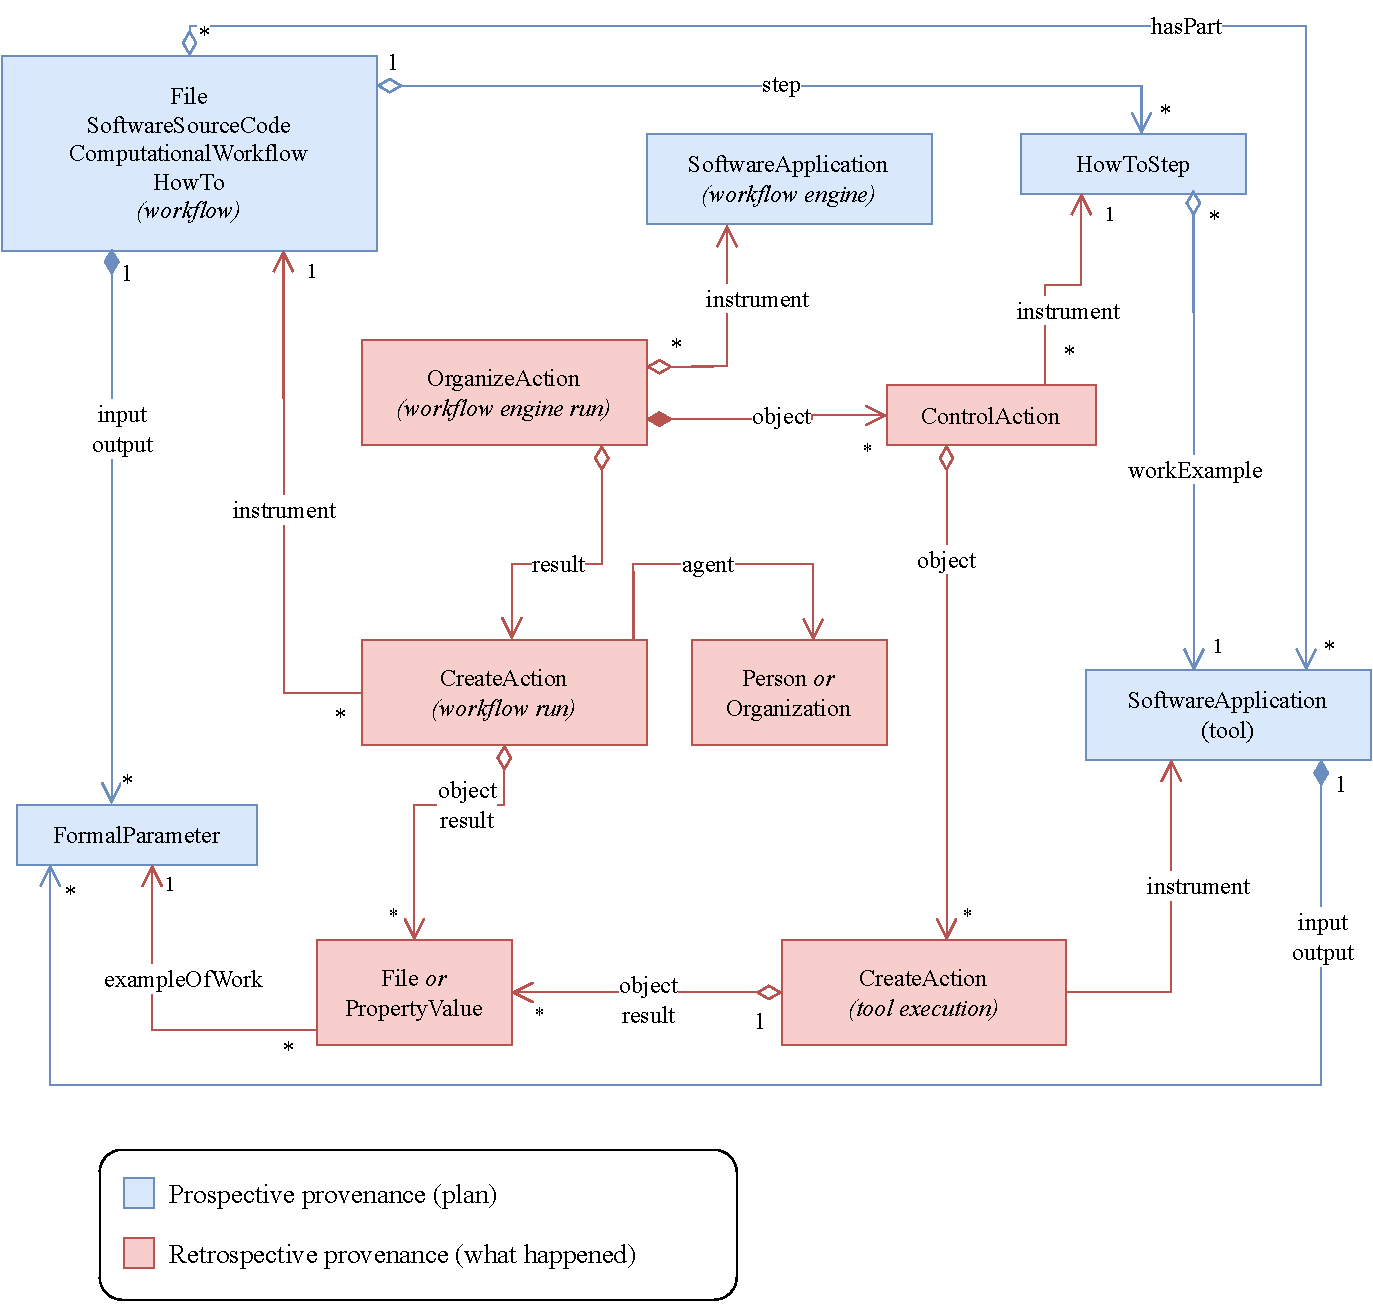
\includegraphics[width=15cm]{figures/ch54/wrroc-figure3.drawio.pdf}
    \caption[UML class diagram for Provenance Run Crate]{{\bf UML class diagram for Provenance Run Crate.}
    In addition to the workflow run, this profile represents the execution of individual steps and their related tools.}
    \label{ch54:fig:provenance_crate_er}
  \end{center}
\end{figure}

This profile also includes specifications on how to describe connections between parameters.
Parameter connections -- a fundamental feature of computational workflows -- describe (i) how tools take as input the intermediate outputs generated by other tools and (ii) how workflow-level parameters are mapped to tool-level parameters.
For instance, consider again the workflow depicted in Fig. ~\vref{ch54:fig:head_sort},
and suppose it is implemented in a workflow language such as CWL. Then the workflow-level input (a text file) is connected to the input of the “head” tool wrapper, and the output of the latter is connected to the input of the “sort” tool wrapper.


A representation of parameter connections is particularly useful for traceability, since it allows to document the inputs and tools on which workflow outputs depend.
Since the current RO-Crate context has no suitable terms for the description of such relationships, 
we added appropriate ones to the aforementioned  ``workflow-run'' context extension (the \url{https://w3id.org/ro/terms/workflow-run\#} namespace):
a \emph{ParameterConnection} type with
\emph{sourceParameter} and \emph{targetParameter} attributes that respectively map to the source and target formal parameters, and a
\emph{connection} property to link from the relevant step or workflow to the \emph{ParameterConnection} instances.

This profile is the most detailed of the three, and offers the highest level of granularity. Fig.~\vref{ch54:fig:profile_venn} shows the relationship between the specifications of the profiles as a Venn diagram.

\begin{figure}[!h]
  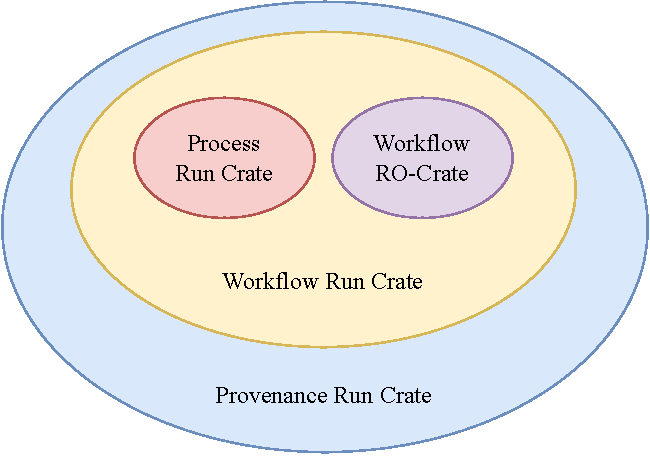
\includegraphics[width=26em]{figures/ch54/wrroc-venn.drawio.pdf}
  \caption[Venn diagram of the specifications for the various RO-Crate profiles]{{\bf Venn diagram of the specifications for the various RO-Crate profiles.}
  Workflow Run Crate inherits the specifications of both Process Run Crate and Workflow RO-Crate. Provenance Run Crate, in turn, inherits the specifications of Workflow Run Crate.}
  \label{ch54:fig:profile_venn}
  \end{figure}


%%
\subsection{Implementations}\label{ch54:implementations}

Support for the Workflow Run RO-Crate profiles presented in this work has been implemented in a number of systems, showing support from the community and demonstrating their usability in practice.
We describe seven of these implementations (one in a conversion tool and six in WMS) in the following sections.
These tools have been developed in parallel by different teams, and independently from each other. 
RO-Crate has a strong ecosystem of tools \cite{Soiland-Reyes 2022}, and these implementations have either re-used these or added their own approach to the standards.



\subsubsection{Runcrate}\label{ch54:runcrate}

Runcrate \cite{runcrate} is a generic Workflow Run RO-Crate toolkit which also serves as a reference implementation of the proposed profiles.
It consists of a Python package with a command line interface, providing a straightforward path to integration in Python software and other workflows.
The runcrate toolkit includes functionality to convert CWLProv ROs to RO-Crates conforming to the Provenance Run Crate profile (\emph{runcrate convert}), effectively providing an indirect implementation of the format for cwltool.
Indeed, the CWLProv model provided a basis for the Provenance Run Crate profile, and the implementation of a conversion tool in runcrate at times drove the improvement and extension of the profile as new requirements or gaps in the old designs emerged.
Runcrate converts both the retrospective provenance part of the CWLProv RO (the RDF graph of the workflow's execution) and the prospective provenance part (the CWL files, including the workflow itself).
Both parts are thus converted into a single, workflow language-agnostic metadata resource.

Another functionality offered by the runcrate package is \emph{runcrate report} which reports on the various executions described in an input RO-Crate, listing their starting and ending times, the values of the various parameters, etc.
Runcrate report demonstrates how the provenance profiles presented in this work enable comparison of runs interoperably across different workflow languages or different implementations of the same language.
This functionality has also been used as a lightweight validator for the various implementations.

We also added a \emph{run} subcommand to re-execute the computation described by an input Workflow Run Crate or Provenance Run Crate where CWL was used as a workflow language.
It works by mapping the RO-Crate description of input parameters and their values (the workflow's
\emph{input} and the action's \emph{object}) to the format expected by CWL, which is then used to relaunch the workflow on the input data.
This functionality shows the machine-actionability of the profiles to support reproducibility, and was used to successfully re-execute the digital pathology annotation workflow described in section \vref{ch54:provenance-run-crate-for-digital-pathology}.

Of course, achieving a full re-execution in the general case may not always be possible: reproducibility is supported by the profiles, but also benefits from the characteristics of the workflow language (which should provide a clear formalism to map input items to their corresponding parameter slots) and from cooperation on the part of the workflow's author, who can help considerably by containerizing the environment required by each step and providing the relevant annotations (if allowed by the workflow language).

\subsubsection{Galaxy}\label{ch54:galaxy}

The Galaxy project~\cite{Galaxy 2022} provides a WMS with data management functionalities as a multi-user platform, aiming to make computational biology more accessible to research scientists that do not have computer programming or systems administration experience.
Galaxy's most prominent features include: a collection of 7500+ integrated \footurl{https://galaxyproject.org/toolshed/}{tools};
a web interface that allows the execution and definition of workflows using the integrated tools; a network of dedicated (public) Galaxy instances.

The export of workflow execution provenance data as Workflow Run Crates has been added in Galaxy's 23.0 release.
This feature provides a more interoperable alternative to the basic export of Galaxy workflow
\emph{invocations}: the workflow definition; a set of serialisations of the invocation-related metadata in Galaxy native, json-formatted files;
and the input and output data files.
This is achieved by extracting provenance from Galaxy entities related to the workflow run, along with associated metadata, converting them to RO-Crate metadata using the ro-crate-py library~\cite{ro-crate-py}; by describing all files contained in the basic invocation export within the RO-crate metadata;
and finally by making the Workflow Run Crate available for export to the user through Galaxy's web interface and API \cite{De Geest 2022}.

We extract the prospective provenance contained in Galaxy's YAML-based \footurl{https://galaxyproject.github.io/gxformat2/v19_09.html}{gxformat2} workflow definition, which includes details of the analysis pipeline such as the graph of tools that need to be executed, and metadata about the data types required.
The retrospective provenance -- i.e., the details of the executed workflow such as the inputs, outputs, parameter values used -- is extracted from Galaxy's data \footurl{https://docs.galaxyproject.org/en/master/lib/galaxy.model.html}{model}, which is not directly accessible to users in the context of a public Galaxy server.
All of this provenance information is then mapped to RO-Crate metadata, including some Galaxy-specific data entities such as dataset collections.
An exemplary exported Galaxy Workflow Run Crate is available on Zenodo~\cite{De Geest 2023b}.

In practice, a user would take the following steps to obtain a Workflow Run Crate from a Galaxy instance: (1) create or download a Galaxy workflow definition (e.g.: from WorkflowHub) and import it in a Galaxy instance, or create a workflow through the Galaxy GUI directly; (2) execute the workflow, providing the required inputs; (3) after the workflow has run successfully, the corresponding RO-Crate will be available for export from the Workflow Invocations list.

\subsubsection{COMPSs}\label{ch54:compss}

COMPSs~\cite{Lordan 2014} is a task-based programming model that allows users to transform a sequential application into a parallel one by simply annotating some of its methods, thus making it efficient to exploit the resources available (either distributed or in a cluster).
When a COMPSs application is executed, a corresponding workflow describing the application's tasks and their data dependencies is dynamically generated and used by the COMPSs runtime to orchestrate the execution of the application in the infrastructure.
As a WMS, COMPSs stands out for its many advanced features that enable applications to achieve fine-grained high efficiency in HPC systems, such as the ability to exploit underlying parallelisation frameworks (i.e.~MPI, OpenMP), compilers (e.g.~NUMBA), failure management, task grouping, and more.

Provenance recording for COMPSs workflows has been explored in previous work~\cite{Sirvent 2022}, where the Workflow RO-Crate profile was adopted in the implementation of a very lightweight approach to document provenance while avoiding the introduction of any significant run time performance overheads.
However, because of the dynamic nature of COMPSs workflows, the Workflow Run Crate profile is better suited to represent them, since workflows are created when the application is executed and, thus, a prior static workflow definition does not exist before that moment.
Due to this limitation, the workflow entity in the metadata file references the entry point application run by COMPSs, and formal parameters are not listed (note that listing them is not required by the profile) because inputs and outputs (both for each task and the whole workflow) are determined at runtime.
COMPSs is able to export provenance data with a post-processing operation that can be triggered at any moment after the application has finished.
The RO-Crate generation post-process uses information recorded by the runtime to detect and automatically add metadata of any input or output data assets used by the workflow.

Implementing Workflow Run Crate support in COMPSs required particular attention to the generation of a unique id for the \emph{CreateAction} representing the workflow run, combining hostname and queuing system job id for supercomputer executions (as extra information added), and just using generated UUIDs for distributed environments, to add as much information as available from the run while ensuring the id is unique.
In the \emph{CreateAction}, the \emph{description} term includes system information, as well as relevant environment variables that provide details on the execution environment (e.g., node list, CPUs per node).
Finally, the \emph{subjectOf} property of the \emph{CreateAction} references the system’s monitoring tool (when available),
where authorised users can see detailed profiling of the corresponding job execution, as provided by the MareNostrum IV \footurl{https://bsc.es/supportkc/docs/MareNostrum4/intro/}{supercomputer}.

To showcase the COMPSs adoption of the Workflow Run Crate profile, we provide as an example the execution of the BackTrackBB~\cite{Poiata 2016}
application in the MareNostrum IV supercomputer.
BackTrackBB targets the detection and location of seismic sources using the statistical coherence of the wave field recorded by seismic networks and antennas.
The resulting RO-Crate~\cite{Poiata 2023} complies with the Workflow Run Crate profile, and includes the application source files, a diagram of the workflow's graph, application profiling and input and output files.

The implementation of provenance recording following Workflow Run Crate has been fully integrated in the COMPSs runtime, and is available since release 3.2 \cite{Ejarque 2023}\footurl{https://github.com/bsc-wdc/compss/tree/3.2}{}.


\subsubsection{StreamFlow}\label{ch54:streamflow}

The StreamFlow framework~\cite{Colonnelli 2020}\footurl{https://github.com/alpha-unito/streamflow}{} is a container-native WMS based on the CWL standard.
It has been designed around two primary principles: first, it allows the execution of tasks in multi-container environments, supporting the concurrent execution of communicating tasks in a multi-agent ecosystem; second, it relaxes the requirement of a single shared data space, allowing for hybrid workflow executions on top of multi-cloud, hybrid cloud/HPC, and federated infrastructures.
StreamFlow orchestrates hybrid workflows by combining a \emph{workflow description} (e.g., a CWL workflow description and a set of input values) with one or more \emph{deployment descriptions} -- i.e.
representations of the execution environments in terms of infrastructure-as-code (e.g., Docker Compose files, HPC batch scripts, and Helm charts).
A streamflow.yml file -- the entry point of each StreamFlow execution -- binds each workflow step with the set of most suitable execution environments.
At execution time, StreamFlow automatically takes care of all the secondary aspects, like scheduling, checkpointing, fault tolerance, and data movements.

StreamFlow stores prospective and retrospective provenance data in a proprietary format into a persistent pluggable database (using sqlite3 as the default choice).
After a CWL workflow execution completes, users can generate an RO-Crate through the \texttt{streamflow prov <workflow\_name>}
command, which extracts the provenance data stored in the database for one or more workflow executions and converts it to an RO-Crate archive that is fully compliant with the Provenance Run Crate Profile, including the details of each task run by the WMS.
Support for the format has been integrated into the main development branch and will be included in release 0.2.0 \cite{Colonnelli 2023b}.

From the StreamFlow point of view, the main limitation in the actual version of the Provenance Run Crate standard is the lack of support for distributed provenance, i.e., a standard way to describe the set of locations involved in a workflow execution and their topology. As a temporary solution,
the StreamFlow configuration and a description of the hybrid execution environment are preserved by directly including the \texttt{streamflow.yml} file into the generated archive.
However, this product-specific solution prevents a wider adoption from other WMS and forces agnostic frameworks (e.g., WorkflowHub) to provide ad-hoc plugins to interpret the StreamFlow format.
Since the support for hybrid and cross-facility workflows is gaining traction in the WMS ecosystem, we envision support for distributed provenance as a feature for future versions of Workflow Run RO-Crate.

\subsubsection{WfExS-backend}\label{ch54:wfexs}

\footurl{https://github.com/inab/WfExS-backend}{WfExS-backend} is a FAIR workflow execution orchestrator that aims to address some of the difficulties found in analysis reproducibility and analysis of sensitive data in a secure manner.
WfExS-backend requires that the software used by workflow steps is available in publicly available software containers for reproducibility.
Actual workflow execution is delegated to one of the supported workflow engines which matches with the workflow, right now either Nextflow or cwltool.
The orchestrator prepares and stages all the elements needed to run the workflow -- i.e. all the files of the workflow itself, the specific version of the workflow engine, the required software containers and the inputs.
All these elements are referred through resolvable identifiers, ideally public, permanent ones.
Due to this, the orchestrator can consume workflows which are originally available in different kinds of locations, like git repositories, Software Heritage, or even RO-Crates from WorkflowHub.

WfExS-backend development milestones aim to reach FAIR workflow execution through the generation and consumption of RO-Crates following the latest Workflow Run Crate profiles, which have proven to be a mechanism suitable to semantically describe digital objects in a way that simplifies embedding key details involved in analysis reproducibility and replicability.

The orchestrator records details relevant to the prospective provenance when a workflow is prepared for execution, such as the public URLs used to fetch input data and workflows, content digestion fingerprints (typically sha256 checksums) and metadata derived from workflow files, container images and input files.
Most of this metadata is represented in the generated RO-Crates. WfExS-backend has explicit commands to generate and publish both prospective and retrospective provenance RO-Crates based on a given existing staged execution scenario.
These RO-Crates can selectively include copies of used elements as payloads.
Workflows can be executed more than once in the same staged directory, with all the executions sharing the same inputs.
Thus, run details from all the executions are represented in the retrospective provenance RO-Crate. Support for Workflow Run RO-Crate is available since WfExS-backend version 0.10.1 \cite{Fernández 2023a}.
Future developments will also add support for embedding URLs of output results that have been deposited into a suitable repository (like Zenodo DOIs, for instance).
Release 1.0 is aiming to include the consumption of previously produced RO-Crates.

An example of Workflow Run Crate generated by WfExS-backend from a Nextflow workflow run \cite{Bouyssié 2023} is available from Zenodo \cite{Fernández 2023b}.

\subsubsection{Sapporo}\label{ch54:sapporo}

Sapporo~\cite{Suetake 2022a} is an implementation of the Workflow Execution Service (WES) API specification \cite{Magee 2018}.
WES is a standard proposed by the Global Alliance for Genomics and Health (GA4GH) for cloud-based data analysis platforms that receive requests to execute workflows.
Sapporo supports the execution of several workflow engines, including cwltool \cite{Amstutz 2023}, Toil \cite{Vivian 2017}, and StreamFlow \cite{Colonnelli 2020}.
Sapporo includes features specifically tailored to bioinformatics applications, including the calculation of feature statistics from specific types of outputs generated by workflow runs.
For example, the system calculates the mapping rate of DNA sequence alignments from BAM format files.
To describe the feature values, Sapporo uses the Workflow Run Crate profile extended with additional terms to represent these biological \footurl{https://github.com/ResearchObject/ro-terms/tree/master/sapporo}{features}.

Further, the Tonkaz companion command line software has integrated functionality to compare Run Crates generated by Sapporo to measure the reproducibility of the workflow outputs~\cite{Suetake 2023}.
Developers can use this unique feature to build a CI/CD platform for their workflows to ensure that changes to the product do not produce an unexpected result.
Workflow users can also use this feature to verify the results from the same workflow deployed in different environments.

While Sapporo supports Workflow Run Crate, since WES is a WMS wrapper, it does not parse the provided workflow definition files. 
Instead, it embeds the information in the files passed by the WES request to record the provenance of execution rather than using the actual workflow parameters meant for the wrapped WMS.
Therefore, the current implementation of Sapporo does not capture the connections between the inputs/outputs depicted in the workflow and the actual files used/generated during the run.
Thus, the profile generated by Sapporo has fields representing input and output files, but they are not linked to formal parameters.

Sapporo supports export to Workflow Run Crate since release 1.5.1 \cite{Suetake 2023b}. An example of RO-Crate generated by Sapporo is available on Zenodo \cite{Ohta 2023}.

\subsubsection{Autosubmit}\label{ch54:autosubmit}

Autosubmit~\cite{Manubens-Gil 2016} is an open source lightweight workflow manager and meta-scheduler created in 2011 for use in climate research to configure and run scientific experiments.
It supports scheduling jobs via SSH to Slurm~\cite{Yoo 2003}, PBS~\cite{Feng 2007} and other remote batch servers used in HPC.

The ``archive'' feature was added in Autosubmit 3.1.0, released in \footurl{https://earth.bsc.es/gitlab/es/autosubmit/-/tags/v3.1.0}{2015}.
This feature archives the experiment directory and all its contents into a ZIP file, which can be used later to access the provenance data or to execute the Autosubmit experiment again.
Even though the data in the ZIP file includes prospective provenance and retrospective provenance, it contains no structure, and users have no way to tell which is which from just looking at the ZIP file and its contents.

Recent releases of Autosubmit 4 include an updated YAML configuration management system that allows users to combine multiple YAML files into a single unified configuration file.
While this gave users flexibility, it also increased the complexity to track the configuration changes and to relate these to the provenance data.

Another feature added in Autosubmit 4 was the option to use only the experiment manager features of Autosubmit, delegating the workflow execution to a different backend workflow engine, like ecFlow~\cite{Bahra 2011}, Cylc~\cite{Oliver 2023}, or a CWL runner.

In order to give users a more structured way to archive provenance, which includes the complete experiment configuration and the parameters used to generate the unified experiment configuration, and also to allow interoperability between workflow managers, the archive feature received a new flag to generate Workflow Run RO-Crates instead of plain ZIP files.

The prospective provenance data is extracted from the Autosubmit experiment configuration.
This includes the multiple YAML files, and the unified YAML configuration, as well as the parameters used to preprocess each file -- preprocessing replaces placeholders in script templates with values from the experiment configuration.
The retrospective provenance data is included with the RO-Crate archive and includes logs and other traces produced by the experiment workflow.
Both prospective and retrospective provenance data are included in the final RO-Crate JSON-LD metadata file. Autosubmit uses the Workflow Run RO-Crate profile.

As one of the most recent implementations, much of the code added in Autosubmit 4 for RO-Crates was adapted from existing implementations like COMPSs and StreamFlow.
ro-crate-py~\cite{ro-crate-py} was used for the heavy lifting work of creating the RO-Crate archive in Python, and adding information for the JSON-LD metadata.

The main challenges for adopting RO-Crate in Autosubmit were incorporating Autosubmit's ``Project'' feature, and the lack of validation tools and of documentation and examples on how to use the standard with \emph{coarse-grained} workflow management systems (as described in~\cite{Goble 2020}) that do not track inputs and outputs, which is the case of Autosubmit -- as well as Cylc and ecFlow.

A Project in Autosubmit is an abstract concept that has a type and a location.
The type can be Git, Subversion, or Local.
For each type the location represents the URL of a code repository, or a directory on a workstation or HPC file system used to copy the Project and its template scripts (written in Shell, R, or Python) and any other files (input data for a model, extra configuration files, binaries, etc.).
The workflows in Autosubmit have tasks with dependencies to other tasks, and each of these tasks execute one of these template scripts.
The RO-Crate archive generated by Autosubmit includes only the project type and location, and not the complete Project.
This means users have the provenance of the Project, but only those with the correct permissions can access its constituent resources (many applications run with Autosubmit can not be publicly shared without consent).

Validation tools for RO-Crate archives are still under development, and while there is a community-based review process to help and guide new implementations, a tool that others can use as code is written will contribute to a more agile development.

After working with the RO-Crate community on these issues, the Autosubmit team adopted a mixed approach where Autosubmit initialises the JSON-LD metadata from its configuration and local trace files, and the user is responsible for providing a partial JSON-LD metadata object in the Autosubmit YAML configuration.
A pull request was created to ro-crate-py to allow the RO-Crate JSON-LD metadata to be patched by these partial JSON-LD metadata objects.
This way, users are able to provide the missing information from the Autosubmit configuration model, like licence, authors, inputs, outputs, formal parameters, and more.
And by modifying ro-crate-py, future implementers of RO-Crate that have a similar workflow configuration as Autosubmit should be able to re-use it, while also using COMPSs, StreamFlow, Autosubmit, and other implementations as reference.

A workflow was created using an example Autosubmit Project~\cite{Kinoshita 2023} designed using UFZ's mHM (mesoscale Hydrological Model)
\cite{Samaniego 2010,Kumar 2013}. This workflow was used to validate the RO-Crate produced by Autosubmit.
This validation was performed by the Workflow Run RO-Crate community in a public GitHub repository (https://github.com/ResearchObject/workflow-run-crate/) and also using the aforementioned Runcrate.




\subsubsection{Summary of implementations}\label{ch54:implementationsummary}

Table \ref{ch54:implementation_summary_table} shows an overview of the different implementations presented in this section.


\begin{table}[!ht]
  \centering
  \caption{Workflow Run Crate implementations}
  \begin{tabular}{l|l|l|l}
  \hline
  {\bf Impl.} & {\bf Profile} & {\bf Version URL/DOI} &
  {\bf Example}\\
  \hline
  runcrate & Provenance & \footnotesize \cite{runcrate}  & \footnotesize \cite{run-pathology} \\
  Galaxy & Workflow & \footnotesize \cite{Afgan 2023} & \footnotesize \cite{De Geest 2023b} \\
  COMPSs & Workflow & \footnotesize \cite{Ejarque 2023} & \footnotesize \cite{Poiata 2023} \\
  Streamflow & Provenance & \footnotesize \cite{Colonnelli 2023b} & \footnotesize \cite{Colonnelli 2023} \\
  WfExS & Workflow & \footnotesize \cite{Fernández 2023a} & \footnotesize \cite{Fernández 2023b} \\
  Sapporo & Workflow & \footnotesize \cite{Suetake 2023b} & \footnotesize \cite{Ohta 2023} \\
  Autosubmit & Workflow & \footnotesize \cite{Beltrán 2023} & \footnotesize \cite{Kinoshita 2023} \\
  \end{tabular}
  \begin{flushleft} 
    Summary of each WRROC implementation, together with the profiles it implements, the latest software citation and an example crate of its application. Runcrate is a toolkit that converts CWLProv ROs to Provenance Run Crates, while the others are WMS.
  \end{flushleft}
  \label{ch54:implementation_summary_table}
\end{table}
  
  


%% 
\subsection{Exemplary Use Cases}\label{ch54:exemplary-use-cases}

We illustrate Workflow Run RO-Crate on two exemplary use cases, which are similar in terms of application domain -- machine learning-aided tumour detection in human prostate images -- but quite different in the way computations are executed and provenance is represented: in the first, the analysis is conducted by means of a CWL workflow and the outcome is represented with Provenance Run Crate; in the second, a combination of Process Run Crate and CPM RO-Crate is used to represent a sequence of computations linked to their corresponding CPM provenance information.


\subsubsection{Provenance Run Crate for Digital Pathology}\label{ch54:provenance-run-crate-for-digital-pathology}

We present a use case that demonstrates the effectiveness of our most detailed profile Provenance Run Crate at recording provenance data in the context of digital pathology.
More specifically, we demonstrate the generation of RO-Crates to save provenance data associated with the computational annotation of magnified prostate tissue areas and cancer subregions using deep learning models~\cite{Del Rio 2022}.
The image annotation process is implemented in a CWL workflow consisting of three steps, each executing inference on an image using a deep learning model: inference of a low-resolution tissue mask to select areas for further processing;
high-resolution tissue inference on areas identified in the previous step to refine borders; high-resolution cancer identification on areas identified in the first step.
The two tissue inference steps run the same tool, but set different values for the parameter that controls the magnification level.
The workflow is integrated in the CRS4 Digital Pathology \footurl{https://github.com/crs4/DigitalPathologyPlatform}{Platform}, a web-based platform to support clinical studies involving the examination and/or the annotation of digital pathology images.

To assess the interoperability of the format, using the same exemplary workflow we implemented provenance recording on two different execution platforms.
In the first case, the workflow was executed with the StreamFlow WMS, for which the Provenance Run Crate implementation is discussed in Section \vref{ch54:streamflow}.
In the second case, we executed the CWL workflow with cwltool and converted the resulting CWLProv RO to a Provenance Run Crate with the runcrate tool (Section \vref{ch54:runcrate}).

The RO-Crates obtained in the two cases~\cite{Colonnelli 2023, run-pathology}
are very similar to each other, differing only in a few details: for instance,~\cite{Colonnelli 2023} includes the StreamFlow configuration file and has separate files for the workflow and the two tools, while
\cite{run-pathology} has the workflow and the tools stored in a single file (CWL's ``packed'' format).
Apart from these minor differences, the description of the computation is essentially the same.
Four actions are represented: the workflow itself, the two executions of the tissue extraction tool and the execution of the tumour classification tool.
Each action is linked to the corresponding workflow or tool via the
\emph{instrument} property, and its starting and ending time are recorded; for each action, input and output slots are referenced by the workflow, while the corresponding values are referenced by the action itself.
The data entities and \emph{PropertyValue} instances corresponding to the input and output values link to the corresponding parameter slots via the \emph{exampleOfWork} property, providing information on the values taken by the parameters.
The listing below (Fig~\ref{ch54:lst:ml_pipeline_streamflow_report}) shows the output of the
\texttt{runcrate report} command for the StreamFlow RO-Crate. 
For each action (workflow or tool run), the tool reports the associated instrument (workflow or tool), the starting and ending time and the list of inputs and outputs, with arrows pointing from the formal parameter to the corresponding actual value taken during the execution of the action.

\begin{listing}
\begin{footnotesize}
\begin{verbatim}
  action: #30a65cba-1b75-47dc-ad47-1d33819cf156
  instrument: predictions.cwl (['SoftwareSourceCode', 
         'ComputationalWorkflow', 'HowTo', 'File'])
  started: 2023-05-09T05:10:53.937305+00:00
  ended: 2023-05-09T05:11:07.521396+00:00
  inputs:
    #af0253d688f3409a2c6d24bf6b35df7c4e271292 <- predictions.cwl#slide
    tissue_low <- predictions.cwl#tissue-low-label
    9 <- predictions.cwl#tissue-low-level
    tissue_low>0.9 <- predictions.cwl#tissue-high-filter
    tissue_high <- predictions.cwl#tissue-high-label
    4 <- predictions.cwl#tissue-high-level
    tissue_low>0.99 <- predictions.cwl#tumor-filter
    tumor <- predictions.cwl#tumor-label
    1 <- predictions.cwl#tumor-level
  outputs:
    06133ec5f8973ec3cc5281e5df56421c3228c221 <- predictions.cwl#tissue
    4fd6110ee3c544182027f82ffe84b5ae7db5fb81 <- predictions.cwl#tumor
action: #457c80d0-75e8-46d6-bada-b3fe82ea0ef1
  step: predictions.cwl#extract-tissue-low
  instrument: extract_tissue.cwl (['SoftwareApplication', 'File'])
  started: 2023-05-09T05:10:55.236742+00:00
  ended: 2023-05-09T05:10:55.910025+00:00
  inputs:
    tissue_low <- extract_tissue.cwl#label
    9 <- extract_tissue.cwl#level
    #af0253d688f3409a2c6d24bf6b35df7c4e271292 <- extract_tissue.cwl#src
  outputs:
    6b15de40dd0ee3234062d0f261c77575a60de0f2 <- extract_tissue.cwl#tissue
action: #d09a8355-1a14-4ea4-b00b-122e010e5cc9
  step: predictions.cwl#extract-tissue-high
  instrument: extract_tissue.cwl (['SoftwareApplication', 'File'])
  started: 2023-05-09T05:10:58.417760+00:00
  ended: 2023-05-09T05:11:03.153912+00:00
  inputs:
    tissue_low>0.9 <- extract_tissue.cwl#filter
    6b15de40dd0ee3234062d0f261c77575a60de0f2 <- extract_tissue.cwl#filter_slide
    tissue_high <- extract_tissue.cwl#label
    4 <- extract_tissue.cwl#level
    #af0253d688f3409a2c6d24bf6b35df7c4e271292 <- extract_tissue.cwl#src
  outputs:
    06133ec5f8973ec3cc5281e5df56421c3228c221 <- extract_tissue.cwl#tissue
action: #ae2163a8-1a2a-4d78-9c81-caad76a72e47
  step: predictions.cwl#classify-tumor
  instrument: classify_tumor.cwl (['SoftwareApplication', 'File'])
  started: 2023-05-09T05:10:58.420654+00:00
  ended: 2023-05-09T05:11:06.708344+00:00
  inputs:
    tissue_low>0.99 <- classify_tumor.cwl#filter
    6b15de40dd0ee3234062d0f261c77575a60de0f2 <- classify_tumor.cwl#filter_slide
    tumor <- classify_tumor.cwl#label
    1 <- classify_tumor.cwl#level
    #af0253d688f3409a2c6d24bf6b35df7c4e271292 <- classify_tumor.cwl#src
  outputs:
    4fd6110ee3c544182027f82ffe84b5ae7db5fb81 <- classify_tumor.cwl#tumor
\end{verbatim}
\caption[runcrate report command line output]{\textbf{runcrate report command line output}.
This informal listing of relevant RO-Crate entities describe each step execution.
Note that inputs and outputs are of different types (not shown), e.g. \texttt{tissue\_low>0.9} is a string parameter, \texttt{6b15de…} is a filename, and \texttt{\#af0253…} is a collection.}
\end{footnotesize}
\label{ch54:lst:ml_pipeline_streamflow_report}
\end{listing}


The \emph{exampleOfWork} link between input / output values and parameter slots is used by \texttt{runcrate run} to reconstruct the CWL input parameters document needed to rerun the computation.
The
\emph{alternateName} property (a Schema.org property applicable to all entities), which records the original name (i.e., at the time the computation was run) of data entities, is also crucial for reproducibility in this case: both StreamFlow and CWLProv, to avoid clashes, record input and output files and directories using their SHA1
checksum as their names. 
However, this particular workflow expects the input dataset to be in the \footurl{https://openslide.org/formats/mirax/}{MIRAX} format, where the ``main'' file taken as an input parameter by the processing application must be accompanied by a directory in the same location with the same name apart from the extension.
The runcrate tool uses the \emph{alternateName} to rename the input dataset as required, so that the expected pattern can be picked up by the workflow during the re-execution.
This use case was the main motivation to include a recommendation to use \emph{alternateName} with the above semantics in Process Run Crate.

Thanks to the fact that both RO-Crates were generated following the best practices to support reproducibility mentioned in the profiles, we were able to re-execute both computations with the runcrate tool.
This was also made possible by the fact that the CWL workflow included information on which container images to use for each tool.
Overall, this shows how reproducibility is a hard-to-achieve goal that can only be supported, but not ensured, by the profiles, since it also depends on factors like the characteristics of the computation, the choice of workflow language and whether best practices such as containerisation are followed.

This use case highlighted the need to add specifications on how to represent multi-file datasets \cite[section Representing multi-file objects]{WRROC 2023a}. In the MIRAX format, in fact, the ``main'' file must be accompanied by a directory in the same location containing additional files with a specific structure.
To represent this, we added specifications to the Process Run Crate profile on describing “composite” datasets consisting of multiple files and directories to be treated as a single unit -- as opposed to more conventional input or output parameters consisting of a single file. The profile specifies that such datasets should be represented by a \emph{Collection} entity linking to individual files and directories via the \emph{hasPart} property, and referencing the main part (if any) via the \emph{mainEntity} property. Note that, by adding this specification to Process Run Crate, we also made it available to Workflow Run Crate and Provenance Run Crate. In the output of the runcrate report tool the additional files are not shown, since the formal parameter points to the \emph{Collection} entity that describes the whole dataset.

\subsubsection{Process Run Crate and CPM RO-Crate for cancer detection}\label{ch54:process-run-crate-and-cpm-ro-crate-for-cancer-detection}
This section presents an RO-Crate created to describe an execution of a computational pipeline that trains AI models to detect the presence of carcinoma cells in high-resolution digital images of magnified human prostate tissue.
The RO-Crate makes use of Process Run Crate and CPM RO-\footurl{https://w3id.org/cpm/ro-crate}{Crate}, an RO-Crate profile that supports the representation of entities described according to the Common Provenance Model (CPM) \cite{Wittner 2022,Wittner 2023b}. 
The CPM, an extension of the W3C PROV model \cite{Moreau 2013} is a recently developed provenance model that enables the representation of distributed provenance. 
Distributed provenance is created when an object involved in the research process, either digital or physical (e.g., biological material), is exchanged between organisations, so that each organisation can document only a portion of the object’s life cycle. 
Individual provenance components are generated, stored, and managed individually by each organisation, and are linked together in a chain. 
The CPM prescribes how to represent such provenance, and how to enable its traversal and processing using a common algorithm, independently from the type of object being described. 
In addition, the CPM defines a notion of meta-provenance, which contains metadata about the history of individual provenance components. 
CPM RO-Crate supports the identification of CPM-based provenance and meta-provenance files within an RO-Crate, allowing to pack data, metadata, and CPM-based provenance information together. 
An RO-Crate generated according to the CPM-RO-Crate profile embeds parts of the distributed provenance, which may be linked to the provenance of precursors and successors of the packed data. 
The CPM-RO-Crate profile synergises well with Process Run Crate, since the former can add references to CPM-based provenance descriptions of computational executions described with the latter, integrating them in the distributed provenance. Since CPM-based provenance and meta-provenance files are typically themselves produced by computations, Process Run Crate allows to represent these along with the main computations that produce the datasets being exchanged, providing the full picture in a cohesive ensemble.


The pipeline consists of three main computational steps: a preprocessing step that splits input images into small patches and divides them into a training and a testing set; a training step that trains the model to recognise the presence of carcinoma cells in the images; an evaluation step that measures the accuracy of the trained model on the testing set.
In addition to the pipeline steps, the RO-Crate describes additional computations related to the generation of the CPM provenance and meta-provenance files.
All computations are described according to the Process Run Crate profile, while the CPM files are referenced according to the CPM RO-Crate profile. 
%(section \namevref{ch54:synergy-with-the-cpm-ro-crate-profile}).
Also represented via Process Run Crate are: the input dataset; the results of the pipeline execution; the scripts that implement the pipeline; the log files generated by the scripts; a script that converts the logs into the CPM files.
This allowed us to describe all involved elements as a single aggregate, with entities and their relationships represented according to the RO-Crate model.
The RO-Crate discussed here is available from Zenodo~\cite{Wittner 2023c}.

The CPM files complement the RO-Crate with internal details about the pipeline execution, such as how the input dataset was split into training and testing sets, or detailed information about each training iteration of the AI model.
For instance, it contains a representation of a checkpoint of the AI model after the second training iteration.
The corresponding entity's attributes contain paths to the respective model stored as a file.
The entity is related to the respective training iteration activity, which contains the iteration parameters represented as an attribute list.
In addition, the CPM generally provides means to link the input dataset provenance to the provenance of its precursors -- human prostate tissues and biological samples the tissues were derived from; this is not included in the example because we used a publicly available input database for which provenance of the precursors was not available.
However, the linking mechanism for provenance precursors is exactly the same as between the bundles for the AI pipeline parts.
While the RO-Crate is focused on the execution of the pipeline, the provenance included in the CPM files intends to be interlinked with provenance of the precursors or successors, providing means to traverse the whole provenance chain.
For the described digital pathology pipeline, the precursors would be: (1) a biological sample acquired from a patient; (2) slices of the sample processed and put on glass slides; (3) the images created as a result of scanning the slides using a microscope.
As a result, combining the CPM and RO-Crate enables the lookup of research artefacts related to the computation across heterogeneous organisations using the underlying provenance chain.


\subsection{Discussion}\label{ch54:discussion}

The RO-Crate profiles presented here provide a unified data model to describe the prospective and retrospective provenance of the execution of a computational workflow, together with contextual metadata about the workflow itself and its associated entities (inputs, outputs, code, etc.). 
The profiles are flexible, allowing to tailor the description to a broad variety of use cases, agnostic with respect to the WMS used and allow describing provenance traces at different levels of granularity. 
This facilitates developing implementations by multiple workflow systems (often with heterogeneous assumptions and requirements) -- six of which have already been developed and are described in Section \vref{ch54:implementations} -- allowing to perform comparisons between runs across heterogeneous systems.
For instance, the \footurl{https://www.w3.org/TR/sparql11-overview/}{SPARQL} query in listing \vref{ch54:sparql} returns all actions in a Workflow Run RO-Crate, together with their instruments and their starting and ending times:

\begin{listing}
\begin{verbatim}
PREFIX schema: <http://schema.org/>
SELECT ?action ?instrument ?start ?end
WHERE {
  ?action a schema:CreateAction .
  ?action schema:instrument ?instrument .
  OPTIONAL { ?action schema:startTime ?start } .
  OPTIONAL { ?action schema:endTime ?end }
}
\end{verbatim}
\caption{SPARQL query to find actions in a Workflow Run RO-Crate}
\label{ch54:sparql}
\end{listing}

Additionally, having workflow runs and plans described according to the RO-Crate model allows to capture the context of the workflow itself (e.g.~authors, related publications, other workflows, etc.) rather than the trace alone. 
Being based on RO-Crate, the profiles and their implementations are part of a growing ecosystem of tools and services maintained by the RO-Crate \footurl{https://www.researchobject.org/ro-crate/in-use/}{community}.
The Workflow Run Crate and Provenance Run Crate profiles are also compatible with the WorkflowHub registry, allowing workflow runs created with those profiles to be registered and easily found and shared with other researchers.

The Workflows Community Summit \cite{Ferreira 2022} identified as one of the current open challenges in the Scientific Workflows domain the ability to build FAIR into Workflow Management Systems, with the objective of achieving FAIR Computational Workflows. The profiles introduced in this article are able to help to tackle this by introducing interoperable metadata among WMSs that captures the provenance of their corresponding workflow executions.

The Workflow Run RO-Crate profiles, the associated tooling, the implementations and the examples are developed by a community that runs regular virtual meetings (every two weeks at the time of writing) and coordinates on Slack and the RO-Crate mailing list.
The WRROC community brings together members of the RO-Crate community~\cite{Soiland-Reyes 2022}, WMS users and developers, Workflow users and developers, GA4GH~\cite{Rehm 2021} Cloud developers and provenance model authors, and is open to anyone who is interested in the representation of workflow provenance.
The inclusion of WMS developers and workflow users was key to keeping the specifications flexible, easy to implement and grounded on real use cases, while the diversity of the stakeholders allowed to keep a plurality of viewpoints while driving the model's development forward.

One of the main benefits of this development process is that the profiles are already in use, with several implementations already available as described in section \vref{ch54:implementations}.

In the following subsections, we illustrate how the model relates to W3C PROV and to other community projects.

\subsubsection{Evaluation of metadata coverage using runcrate convert}

In order to assess the metadata coverage of runcrate, we performed a qualitative analysis of the tool's \emph{convert} mode, in which we evaluated how the generated RO-Crates preserve the metadata contained in the CWLProv ROs from which they are derived.
For this analysis, we followed the same approach as for an earlier evaluation of CWLProv~\cite{De Wit 2022}.
We identified and analysed three levels of representation:
firstly, in RDF; secondly, in a structured, but CWL-specific document;
and finally, in an unstructured, human readable format.
From this earlier analysis, we concluded that the CWLProv RDF representation of the workflow runs lacked many provenance metadata that was included in CWL-specific documents, such as the packed workflow and input parameter file.
For example, the CWLProv RDF only contained the name of each workflow step, without including the link to the underlying CommandLineTool or nested Workflow that was executed; information that could be extracted from the packed workflow.

In our analysis of runcrate, we compared the CWLProv RDF provenance graph with the RO-Crate metadata file.
Because runcrate only generates RO-Crates \emph{after} workflow execution, we only considered components that in CWLProv were at least partially represented in structured format (CWL-specific or RDF), and analysed their presence in RDF in RO-Crate (the packed CWL workflow is identical between CWLProv and RO-Crate).

The results of the analysis are summarised in Table
\vref{ch54:analysis_table}.
Overall, most of the information contained in CWLProv RDF is transferred to the RO-Crate metadata.
In addition, the representation of some categories of metadata has improved, notably Workflow parameters (WF2), which were insufficiently described in CWLProv RDF but defined with type and format in RO-Crate.
Moreover, the format of input files (D2), which was absent in CWLProv RDF, is represented in RO-Crate.

In conclusion, our analysis shows that runcrate preserves most provenance metadata previously shown to be relevant in realistic RO use case scenarios.
The full results of the analysis can be found at \cite{de Wit 2023}.


% Place tables after the first paragraph in which they are cited.
\begin{table}[!ht]
\centering
\caption{
Summarised results of our qualitative analysis of runcrate.}
\begin{tabular}{r|l|l|c|c|c|c}
\hline
%% TODO: Check ticks are in right places
{\bf Type} & {\bf Subtype} & {\bf Name} & {\bf CWL} & {\bf CWLProv} & {\bf RO-Crate} & {\bf WRROC}  \\ \hline
T1 & SC1 & Workflow design & $\bullet$ &  $\cdot$  &  $\cdot$ & $\dots$ \\ 
& SC2 & Entity annotations & $\circ$ &  $\cdot$  &  $\cdot$  & $\dots$ \\ 
& SC3 & Workflow execution ann.  &  $\circ$  & $\cdot$ &  $\cdot$ & $\dots$ \\ \hline
T2 & D1 & Data identification & $\circ$ & $\cdot$ &  $\cdot$ & $\dots$ \\
& D2 & File characteristics & $\circ$ & $\cdot$ & $\circ$ & $\circ$ \\
& D3 & Data access & $\circ$ &  $\cdot$  &  $\cdot$  & $\dots$ \\ 
& D4 & Parameter mapping & $\bullet$ & $\bullet$ & $\bullet$ & $\bullet$ \\ \hline 
T3 & SW1 & Software identification & $\circ$ &  $\cdot$ & $\cdot$ & $\dots$ \\ 
& SW2 & Software documentation & $\circ$ &  $\cdot$ & $\cdot$ & $\dots$ \\  
& SW3 & Software access & $\circ$ &  $\cdot$ & $\cdot$ & $\dots$ \\ \hline 
T4 & WF1 & Workflow software & $\circ$ & $\circ$ & $\circ$ & $\dots$ \\ 
& WF2 & Workflow parameters & $\circ$ & $\circ$ & $\bullet$ & $\bullet$ \\ 
& WF3 & Workflow requirements & $\dots$ &  $\cdot$  &  $\circ$  & $\dots$ \\ \hline 
T5 & ENV1 & Software environment & $\dots$ & $\cdot$ &  $\cdot$ & $\dots$ \\ 
& ENV2 & Hardware environment & $\dots$ & $\cdot$ &  $\cdot$  & $\cdot$\\ 
& ENV3 & Container image & $\circ$ & $\circ$ &  $\circ$ & $\bullet$ \\ \hline 
T6 & EX1 & Execution timestamps & $\cdot$ & $\bullet$ & $\bullet$ & $\bullet$ \\ 
& EX2 & Consumed resources &  $\cdot$ & $\cdot$ & $\cdot$ & $\cdot$  \\ 
& EX3 & Workflow engine & $\cdot$ & $\circ$ & $\circ$ & $\circ$  \\  
& EX4 & Human agent & $\circ$ & $\bullet$ & $\bullet$ & $\bullet$ \\ \hline
\end{tabular}
\begin{flushleft} We compared RO-Crates with the CWLProv ROs from which they were generated.
The analysis was based on a provenance taxonomy reflecting relevant provenance metadata based on realistic use cases for ROs associated with a real-life bioinformatics workflow.
We only considered provenance metadata which was already represented in CWLProv RDF or CWL-specific documents (\texttt{packed.cwl}, \texttt{primary-job.json}, and \texttt{primary-output.json}).
Since \texttt{packed.cwl} is also included in RO-Crate, we only considered how the metadata was represented in \texttt{ro-crate-metadata.json}.\\
For completeness we also show the theoretical capability of the Provenance Run Crate profile (WRROC column) assuming only its MUST/SHOULD requirements are complete.\\
\textbf{Legend:} $\bullet$ fully represented  $\;\;\circ$ partially represented  $\;\;\dots$ optional (e.g. schema.org attribute) $\;\;\cdot$ missing or unstructured representation
\end{flushleft}
\label{ch54:analysis_table}
\end{table}

From this analysis it is worth highlighting the gaps and potential for Workflow Run RO-Crates. Several areas have been flagged by this study as important aspects of workflow metadata, such as Data Access (D3), Software Documentation (SW2) and Workflow Requirements (WF3). The … in the WRROC column indicates these are possible to describe in an RO-Crate using existing schema.org vocabulary (e.g. \url{http://schema.org/softwareHelp}) but are not required by WRROC profiles. Additionally many such aspects require human annotation and cannot be provided by workflow engines alone, although they may be propagated from workflow and tool definitions. Some areas like Consumed Resources (EX2) require additional terms to be defined.


\subsubsection{Workflow Run RO-Crate and the W3C PROV standard}

Our aim is to be compatible with both Schema.org and W3C PROV. Provenance Run Crate is the profile that most closely matches the level of detail provided by CWLProv, which extends W3C PROV. Table \vref{ch54:rocrate_prov_mapping} shows how the main entities and relationships represented by Provenance Run Crate map to PROV constructs. A machine-readable version of the mapping can be found \footurl{https://github.com/ResearchObject/workflow-run-crate-paper/tree/main/mapping}{online}.
% TODO: Update to w3id PID

\begin{table}[!ht]
  \centering
  \caption[Mapping from Workflow Run RO-Crate to equivalent W3C PROV concepts]{
  {\bf Mapping from Workflow Run RO-Crate to equivalent W3C PROV concepts} using SKOS \cite{w3-skos-primer}. For instance, \emph{CreateAction} has \textbf{broader} match PROV's \emph{Activity}, meaning that \emph{Activity} is more general.}
  \begin{tabular}{p{35mm}|p{40mm}|p{40mm}}
  \hline
%  {\bf W3C PROV} & {\bf RO-Crate} & \textbf{Relationship} \\
  {\bf RO-Crate} & \textbf{Relationship} & {\bf W3C PROV-O} \\
  \hline

  \emph{Action} (superclass of \emph{CreateAction}, \emph{OrganizeAction}) & 
    Has close match 
    \begin{small}
      (schema.org Actions may also be potential actions in the future)
    \end{small}
    & 
    \emph{Activity}
    \\ \hline
  \emph{CreateAction}, \emph{OrganizeAction} & 
    Has broader match & 
    \emph{Activity}
    \\ \hline
  \emph{Person} & 
    Has exact match & 
    \emph{Person}
    \\ \hline
  \emph{Organization} & 
    Has exact match & 
    \emph{OrganizeAction} 
    \\ \hline
  \emph{SoftwareApplication} & 
    Has related match & 
    \emph{SoftwareAgent}
    \\ \hline
  \emph{ComputationalWorkflow}, \emph{SoftwareApplication}, \emph{HowTo} & 
    Has broader match & 
    \emph{Plan},
    \emph{Entity}
    \\ \hline
  \emph{File}, \emph{Dataset}, \emph{PropertyValue} & 
    Has broader match & 
    \emph{Entity}
    \\ \hline
  \emph{startTime} on \emph{CreateAction} & 
    Has close match & 
    \emph{startedAtTime}
    \\ \hline
  \emph{endTime} on \emph{CreateAction} & 
    Has close match & 
    \emph{endedAtTime}
    \\ \hline
  \emph{agent} on \emph{CreateAction} & 
    Has related match & 
    \emph{wasStartedBy}, \emph{wasEndedBy}
    \\ \hline
  \emph{agent} and \emph{instrument} on \emph{CreateAction} & 
    Has broader match & 
    \emph{wasAssociatedWith}
    \\ \hline
  \emph{instrument} on \emph{CreateAction} & 
    Has related match 
    \begin{small}
      (Complex mapping: an instrument implies a qualified association with the agent, linked to a plan)
    \end{small}
    & 
    \emph{hadPlan} on \emph{Association}
    \\ \hline

  \emph{object} on \emph{CreateAction} &
    Has exact match & 
    \emph{used} 
    \\ \hline
  \emph{result} on CreateAction & 
    Has close match & 
    inverse \emph{wasGeneratedBy} 
  
  \end{tabular}
  %\begin{flushleft} Table notes \end{flushleft}
  \label{ch54:rocrate_prov_mapping}
\end{table}


\subsubsection{Five Safes Workflow Run Crate}\label{ch54:trusted-workflow-run-crate}

The TRE-FX project \cite{trefx}\footurl{https://trefx.uk/}{} has developed Five Safes RO-Crate \cite{5s-crate}, a profile that extends the Workflow Run RO- Crate profile for use in Trusted Research Environments (TRE) to handle sensitive health data in federated workflow execution across TREs in the UK following the Five Safes Framework \cite{Desai 2016}.
A crate with a workflow run request references a pre-approved workflow and project details for manual and automated assessment according to the TRE's agreement policy for the sensitive dataset. 

The crate then goes through multiple phases internal to the TRE, including validation, sign-off, workflow execution and disclosure control.
At this stage the crate is also conforming to the Workflow Run Crate profile.
The final crate is then safe to be made public.
This extension of Workflow Run Crate documents and supports the human review process -- important for transparency on TRE data usage. 
TRE-FX is implementing this profile using WfExS as the workflow execution backend, and this approach will form the basis for further work on implementing federated workflow execution in the British initiatives DARE UK and HDR UK \cite{Snowley 2023}.   



\subsubsection{Biocompute Object RO-Crate}\label{ch54:bco-crate}

IEEE 2791-2020 \cite{ieee2791}, colloquially \emph{Biocompute Objects} (BCO), is a standard for representing provenance of a genomic sequencing pipeline, intended for submission of the workflow to regulatory bodies, e.g. as part of a personalised medical treatment method \cite{Alterovitz 2018}. 
The BCO is represented as a single JSON file which includes description of the workflow and its steps and intended purpose, as well as references for tools used and data sources accessed. 
There is overlap in the goals of BCO and Workflow Run Crate profiles, however their intentions and focus are different. 
BCO is primarily conveying a computational method for the purpose of manual regulatory review and further reuse, with any values provided as an exemplar run.  
A Workflow Run Crate however is primarily documenting a particular workflow execution, and the workflow is associated to facilitate rerun rather than reuse. 

Previously, a guide to packaging BioCompute Objects using RO-\footurl{https://biocompute-objects.github.io/bco-ro-crate/}{Crate} was developed as a profile to combine both standards \cite{Soiland-Reyes 2021}.
In this early approach, RO-Crate was primarily a vessel to transport the BCO along with its constituent resources, including the workflow and data files, as well as provide these resources with additional typing and licence metadata that is not captured by the BCO JSON. 
Further work is being planned with the BCO community to update the BCO-RO profile to align with the newer Workflow Run Crate profiles. 

\subsection{Conclusion and Future Work}\label{ch54:conclusion}

In this work we presented Workflow Run RO-Crate, a collection of RO-Crate profiles to represent the provenance of the execution of computational workflows at different levels of granularity.
We described each profile and their corresponding implementations, shown how they apply to real use cases and described the community behind their development process.
Workflow Run RO-Crate has already been adopted by six WMS, including Galaxy, StreamFlow and COMPSs. The flexibility of our model eases its implementation in more systems, allowing interoperability between their workflow run descriptions.

Workflow Run RO-Crate is an ongoing project driven by an open community.
A natural consequence of this is that the profiles are not static entities, but keep being updated to cater for new requirements and use cases.
In-progress features are tracked in the GitHub repository issues \footurl{https://github.com/ResearchObject/workflow-run-crate/issues}{section} and are open to discussion for the community.
New features under discussion include a representation of the execution environment and recording workflow resource usage.
The runcrate toolkit is planned to be expanded both to better support the current features and to include new ones that may arise.

Future work for the Galaxy implementation includes adding metadata detailing each step of the workflow run to conform to the Provenance Run Crate profile; developing and/or integrating RO-Crate more deeply with import and export of Galaxy histories through the implementation of a profile; further developing features to allow for user-guided import of RO-Crates as Galaxy datasets, histories and workflows.

Finally, we are currently exploring the cloud execution of Workflow Run RO-Crates.
On the one hand, the Workflow Execution Service (WES) specification is used by the Global Alliance for Genomics and Health (GA4GH) \cite{Rehm 2021} to enable WMS-agnostic interpretation of workflows and scheduling of task execution. On the other hand, the Task Execution Service (TES) specification enables the execution of individual, atomic, containerized tasks in a compute backend-independent manner.

We are planning to undertake an in-depth analysis of the degree of interoperability between the TES and WES API standards -- roughly the equivalents of Process and Workflow Run Crates, respectively -- by placing their focus on the actual execution of tasks/processes and workflows in cloud environments and liaising with the GA4GH Cloud community to align schemas where necessary.
We will then build an interconversion library that attempts to (1) construct WES workflow and TES task run requests from RO-Crates containing Provenance, Workflow or Process Run requests and therefore allow their easy (re)execution on any GA4GH Cloud API-powered infrastructure, and (2) bundle information from the WES and TES (as well as other GA4GH Cloud API resources, where available) to create or extend RO-Crates with standards-compliant Process, Workflow or even Provenance RO-Crates.



\chapter{Discussion and conclusions}
\label{chapter:conclusions}
\section{Discussion}
\label{ch61:discuss}

In this section I summarise and discuss the findings from the previous chapters, relating them to emerging related work and future directions.

\subsection{Making a predictable ecosystem of FAIR digital objects}
\label{ch61:ecosystem}

The main advantage of scholarly researchers publishing \emph{FAIR data} is to enable machine actionability \cite{Wilkinson 2016}, which again will accelerate further research, such as through computational workflows. 
In practice, data publishing is largely approached either by depositions in general and institutional repositories for Open Data such as Figshare and Zenodo \cite{Dillen 2019}, or to specialized domain-specific repositories such as in biodiversity \cite{ch8-7}. 

European research infrastructures supporting Open Science practices are coalescing their services to form the European Open Science Cloud (EOSC) \cite{10.2777/940154}, which are embracing FAIR principles \cite{Mons 2017} and building a common framework for interoperability \cite{eosc-interop-framework}. 

While existing practices for implementing FAIR have relied on the Linked Data stack, that is just one possible technology to achieve the benefits of interoperable machine actionability \cite{Mons 2017}. 

Chapter \ref{chapter:fdo} explored the emerging concept of \emph{FAIR Digital Objects} (FDO) \cite{Schultes 2019} as a potential distributed object system for FAIR data, comparing its proposed principles and current practices with the established Linked Data approach. 
As detailed in section \vref{ch3:fdo}, FDO defines a handful of constraints and guides for a predictable way to organise complex machine actionable digital entities. 

Conceptually FDO can clearly be useful for realizing FAIR principles with more active digital objects that can form a consistent ecosystem, but this opens many questions on actual FDO implementations with regards to protocols and standards.

\subsubsection{Linked Data need more constraints and consistency to be FAIR}
\label{ch61:constraints}

Examined in section \vref{ch3:ld}, the principles of \emph{Linked Data} emerged from the Semantic Web as a data-centric view with a focus on navigation and cross-site interoperability, rather than say elaborate logical inferencing systems using ontologies.  
Yet the bewildering landscape of technology choices for using RDF in data platforms means that the developers suffer and still face a steep learning curve. 
For clients consuming Linked Data from multiple sources -- \emph{Linked Data Mashup} \cite{Tran 2014} -- the situation is still baffling in that relatively small differences in identifiers, vocabularies and usage patterns across deployment result in incompatibilities that may require platform-specific workarounds and mappings \cite{Millard 2010}. 

The ecosystem of FAIR tooling is not currently mature enough to support Linked Data consumption in a user-friendly and efficient way \cite{Thompson 2020}, although recent metrics and tools for assessing \emph{FAIRness} \cite{Wilkinson 2018} can assist both data providers and consumers. 
Evaluations by EOSC has since found that FAIRness metrics can vary widely across the different assessment tools for the same data resource \cite{10.5281/zenodo.7463421}, showing that further definitions of conventions and practices are needed for consistent Linked Data publishing and consumption. 

Making the FAIR principles achieve practical benefits for researchers and platform developers thus requires more specific constraints and broader consistency.

\subsubsection{FDOs as a distributed object system on the Web}
\label{ch61:distributed}

The framework-based comparisons in section \vref{ch3:results} considered the implementation details of both FDO and Linked Data, and evaluated to what extent either can be considered a global distributed object system. 
The findings from this research show that FDO recommendations can benefit FAIR thinking to build machine actionable ecosystems and provide stronger promises of consistency and predictability across data platforms. 

These comparisons highlighted that the Web on the other hand has a flexible, scalable and mature technology stack, which can form a solid basis for implementing FDO. 
However, if such implementation is to use Linked Data technologies, these must be constrained sufficiently in order to practically realize such an ecosystem within the FDO guidelines and without degrading the developer experience.


\subsubsection{FDOs can be implemented on the Web using Signposting}
\label{ch61:signposting}

Section \vref{ch2:meeting-fdo-principles-using-linked-data-standards} explored how the FDO principles can be achieved for Linked Data as further constraints on existing standards.
As chapter \ref{chapter:fdo} has highlighted throughout, there are many technical details remaining to be specified for FDO it to be consistently implemented according to its own principles.

If such conventions need to be evolved and specified no matter the protocol basis for FDO, this chapter argued, then it would be intuitive to build FDO on the mature Web stack, unless there was an compelling argument for alternative protocol stacks having other advantages.\footnote{
  For instance, a de-centralized, resiliant architecture and long term preservation was the motivation for the design of the Interplanetary File System (IPFS) as a \emph{Decentralized Web} \cite{Trautwein 2022}.
}

Section \ref{ch2:discussion} found that the basis of Web-based FDOs can be built using only Signposting \cite{vandesompel2015,Van de Sompel 2022}, adding a couple of non-intrusive HTTP headers that are agnostic to metadata standards and serializations. An implementation of such Web-based FDOs was shown in section \ref{ch4:lightweight-fdo}. 

The Signposting approach has also been highlighted both by EOSC \cite{10.5281/zenodo.7463421} and as a possible FDO configuration type \cite{fdo-ConfigurationTypes}.
The FAIR-IMPACT project launched an \footurl{https://fair-impact.eu/1st-open-call-support-closed}{open call} where 14 participating institutions participated to help build support for Signposting \cite{soilandreyes2023b} in data repositories and platforms.



\subsection{RO-Crate as a developer-friendly approach}
\label{ch61:crate}

As pointed out in section \vref{ch3:ld-web}, while Linked Data is a powerful and flexible approach to publishing structured data on the Web, the developer experience of using Semantic Web technology still needs simplifications, like reducing number of choices for vocabularies and serialization formats. 

Chapter \vref{chapter:ro-crate} introduced \emph{RO-Crate} as a practical implementation of the FAIR principles for the purpose of packaging data alongside structured metadata.
The approach builds on best practices for Linked Data, however RO-Crate specifications are example-driven with simple interrelated JSON structures, and primarily use a single, general purpose vocabulary. 

This way of ``Linked Data by stealth'' means that developers don't need to be concerned about RDF implementation details, although they can at their option take advantage of RDF knowledge graph technologies like SPARQL (section \vref{ch5:linkeddata}).
Extension points are well defined, and although extending RO-Crate do require some RDF knowledge like defining namespaces, reasonable examples and vocabulary repositories are provided by RO-Crate --  developers do not for instance need to learn about ontologies nor need to deploy a web service serving multiple RDF serialisations for every described entity.



\subsubsection{Just enough Linked Data}
\label{ch61:justenough}

An important lesson from this work then is to use ``just enough'' Linked Data for the desired level of interoperability and knowledge representation.
While previous efforts to `FAIRify' largely have been concerned about representing the data values using an RDF data model, this can lead to significant effort needed in developing ontologies and vocabularies. 

RO-Crate is using schema.org \cite{schema.org} as its base vocabulary, and tries to follow its philosophy of building a lightweight semantic structure by associating many free text attributes to the same node, rather than making elaborate interconnected semantic objects.
For instance, while a \texttt{Person}'s \texttt{affiliation} ideally goes to a \texttt{Organization} with it's own URL and other attributes, in some cases, a free text string is all information available, and this can be used cirectly as the \texttt{affiliation}. 

With retrospect we can say that this reduction in semantic rigidity compared to use in OWL ontologies is a move back to the simplicity of early RDF as an open-ended model (see section \vref{ch3:semweb}), where a property can be used to point to almost anything, and RDF authors are free to use almost any term.

Another aspect that is not highlighted well in ontologies is where to stop in the formal knowledge representation of an object.
In schema.org, many properties like \url{http://schema.org/license} are defined as having the \emph{range}\footnote{Expected type of object \cite{w3-rdf-schema}, however note that schema.org uses \url{http://schema.org/rangeIncludes} instead of \texttt{rdfs:range}, to permit multiple alternatives without the need for a union class.} of either \footurl{http://schema.org/CreativeWork}{\texttt{CreativeWork}} or \footurl{http://schema.org/URL}{\texttt{URL}}, hinting that the licence is not required to be explained as another entity with further properties, but that the attribute's primary purpose is navigation or identification. 

This would be a key aspect of Linked Data, which traditionally have had the rather undefined convention of ``follow your nose'' navigation -- a client may attempt to request any node identifier (if it's a URL), and if, with content-negotiation, it returns some RDF, then that could be integrated into a joint knowlege graph, hopefully adding more description of that node, although possibly using other vocabularies.
However, ontologies used in Linked Data have not commonly indicated navigation waypoints as done in Schema.org, simply defining a property's range as a given class leaves it undefined if documents were expected to explain that node or link to its explanation. One notable exception is the Data Catalog Vocabulary (DCAT)\footnote{Although the \url{http://schema.org/Dataset} type used by RO-Crate's root entity is derived from DCAT, RO-Crate does not assume a corresponding data catalogue on the Web.} \cite{DCAT2 2020} which have navigational properties like \texttt{dcat:landingPage} (to a \texttt{foaf:Document}) and \texttt{dcat:downloadURL} (to any \texttt{rdfs:Resource}).

% Should we discuss why not DCAT?

\subsubsection{Embedding contextual information reduces need for navigation}
\label{ch61:contextual}

A divergence from common Linked Data practices is that our RO-Crate approach is making a self-described container.
Rather than assume that information will always be available from the referenced URIs, and requiring clients to crawl their way through the many identifiers to see which ones contain more information, the RO-Crate contains a minimal description of each referenced contextual entity (section \vref{ch5:contextualentities}). 

This has multiple purposes:

\begin{itemize}
    \item Simplify user interfaces, e.g. show a human-readable label and type before the user chooses to click the link.
    \item Vocabulary adaptation, for instance describing with schema.org in the crate, what was expressed in FOAF vocabulary at the URI.
    \item Unify descriptions of semantic artefacts and web pages. 
          Making ``ad-hoc'' semantic artefacts within the crate where none exited beforehand.
    \item Embed ``as of at time of writing'' descriptions for longevity. 
          An RO-Crate is self-contained and can be archived independently, and embedding contextual information reduces cross-organizational service dependencies (at the risk of outdated information).
\end{itemize}

Several of these reasons are also organizational in nature, reflecting back on the EOSC Interoperability Framework (section \vref{ch3:eosc-interoperability-framework}) -- rather than requiring for instance the Research Organization Registry \footurl{https://ror.org/}{(ROR)} to add Linked Data representations of organizations, one can be made ad-hoc by the RO-Crate's author, and contained by the crate as a contextual entity. 

This ability to describe a referenced entity locally is also a workaround for the chicken-and-egg problem of creating and linking Linked Data resources that vocabulary-wise are cross-related both ways. For instance orcid.org recently added schema.org content negotiation, but \emph{after} RO-Crate started describing people using the \url{http://schema.org/Person} type and ORCID identifiers.\footnote{
  One of my earlier code contributions to ORCID already established content-negotiation to RDF -- but using the classical FOAF vocabulary \cite{FOAFVocabularySpecification}.
  Slightly inconsistent with Semantic Web principles, the registry is currently returning \emph{Person} descriptions in different semantic models depending on the requested serialization. \\
  \url{https://github.com/ORCID/ORCID-Source/blob/main/CONTENT_NEGOTIATION.md}} 


\subsubsection{FDO ecosystems need to permit flexible references}
\label{ch61:references}

When reflecting on the above contextualization from the propositions of FAIR Digital Objects as covered back in chapter \ref{chapter:fdo}, we can predict a problem if every reference from an FDO must go to another pre-existing FDO (or at least a registered PID), in that there must then be a linear order of FDO creation within an ecosystem of compatible FDO types.
A strict reading of the FDO principles means implementations cannot utilise the established human-readable Web for bootstrapping.
This risks large cross-organizational delays with a stronger need for collaboration and coordination, or alternatively, starting with a smaller FDO data models that can gradually evolve to add more navigation, when and if registries appear with FDO interfaces. 

The emphasis on strong typing in FDOs also means that seemingly incompatible types (for instance developed by the biodiversity community vs. those from genomics communities) lead to a split of the PID space of referencable objects from a given type of FDOs.  Counter to this, the current FDO recommendations for attributes and types \cite{fdo-ImplAttributesTypesProfiles} do not require specification of the \emph{range} of an attribute to be a PID of an FDO, and as current FDO type declarations have been relatively lightweight (textual descriptions only), they are flexible enough to permit URLs to any Web resource or existing Linked Data concepts.  

There is a concern however that some FDO serializations using the Handle system and key-value attributes cannot distinguish between string literals and object references.
Combined with the use of PID references expressed as handles rather than as a URIs (e.g. \texttt{21.14100/2fcf49d3-0608-3373-a47f-0e721b7eaa87} instead of \url{https://hdl.handle.net/21.14100/2fcf49d3-0608-3373-a47f-0e721b7eaa87}), this means that machine actionability suffers, in that the string value is not typed to what kind of reference it may or may not be, or in what PID system. Compare this with listing \vref{ch3:triples} where the RDF syntax distinguishes literal strings from object references -- in Handle-based FDOs, machine-actionable navigation is only possible by understanding the attributes of the FDO type, yet as highlighted in the previous paragraph these type definitions are not directly machine-actionable themselves.

In schema.org we find a similar challenge with properties permitting both string values and object references. \url{http://schema.org/keywords} is perhaps the most ambiguous, as it permits \texttt{Text}\footnote{To conflate matters, the \texttt{keywords} property can be repeated, but also allows multiple keywords within a single comma-separated string.}, but also \texttt{URL} or \texttt{DefinedTerm}.
The two latter cases are both intended for referencing controlled vocabularies, with the distinction that a \texttt{DefinedTerm} is defined explicitly within the referenced object, while the defined term is implied if only the URL is provided.
JSON-LD contexts have the possibility of enforcing object references (\texttt{"@type: "@id"}), but this cannot be used in this case as freetext strings are also permitted.
The result is that a freetext keyword that just looks like a URL cannot be distinguished from an intended URL reference, similar to the FDO Handle example in the previous paragraph.

In order to reduce such ambiguity and multiple developer choices, in RO-Crate all object references are in JSON-LD object form, and the RO-Crate context do not have any \texttt{@type} shortcuts for implicit references.
RO-Crate 1.2 will also recommend that \footurl{https://www.researchobject.org/ro-crate/1.2-DRAFT/metadata.html\#common-principles-for-ro-crate-entities}{all entities} have a type, identifier and human-readable name. 


\subsubsection{Profiles restrict general flexibility to gain specific predictability}
\label{ch61:profiles}

Section \vref{ch5:inuse} showed how RO-Crate is adopted by different scientific domains. 
Since the publication of the corresponding manuscripts in chapter \ref{chapter:ro-crate}, RO-Crate has also been used by the \footurl{https://www.researchobject.org/ro-crate/in-use/LDaCA.html}{Language Data Commons of Australia} \cite{LREC2022} building language corpa, \footurl{https://www.researchobject.org/ro-crate/in-use/survey-ontology.html}{Survey Ontology} \cite{surveyOntology} describing surveys, \footurl{https://nfdi4plants.org/content/learn-more/annotated-research-context.html}{DataPlant} for plant experiments, \footurl{https://w3id.org/cpm/ro-crate}{distributed provenance} of biological specimens \cite{Wittner 2020,Wittner 2023,Wittner 2023b}, \footurl{https://w3id.org/ro/doi/10.5281/zenodo.6913045}{COVID-19 causal inferences} to compare public health interventions internationally \cite{Meurisse 2023}, and \footurl{https://w3id.org/5s-crate/0.4}{Trusted Research Environments} for controlled workflow computation on sensitive health data. Several of these use cases have also expanded RO-Crate with additional terms from schema.org or defined in corresponding RO-Crate profiles. The span of these domains shows that RO-Crate is flexible for a range of use cases and can be adopted by developers not familiar with Semantic Web technologies.

The discussion of strictness vs flexibility in section \vref{ch5:strictness-vs-flexibility} highlighted the tension between a flexible open-ended model and the predictability needed to consistently create and consume content expressed by the model.
While RO-Crate itself can be seen as a restriction of the more open-ended JSON-LD and schema.org, its extensibility points still allow different use cases to expand on those conventions.  

Section \vref{ch5:profiles} detailed how semi-formalized profiles can be gradually formed to at first \emph{duck-type} a class of RO-Crates that have similar properties.
Later work has formalized this as \footurl{https://www.researchobject.org/ro-crate/1.2-DRAFT/profiles}{Profile Crate} to capture the profile itself as a separate crate. This have now evolved to use the W3C Profiles Vocabulary \cite{dx-prof} to explicitly link to vocabularies, mappings and importantly constraints expressed as RDF Shapes \cite{fdo-collections}. 
This turns RO-Crate profiles into machine-actionable type definitions, from which existing RDF tooling can do for instance validation. 
Figure \ref{ch61:fig:profilecrate} shows how the usage of \emph{roles} within the profile crate indicates the purpose of the constituent parts.
Roles are here particularly important as many of these Semantic Web resources are expressed in the same file format (e.g. \texttt{text/turtle}) and may be used for different purposes (e.g.
SKOS is used to represent either a \emph{mapping} or a \emph{vocabulary} \cite{w3-skos-primer}).

\begin{figure}[htb]
    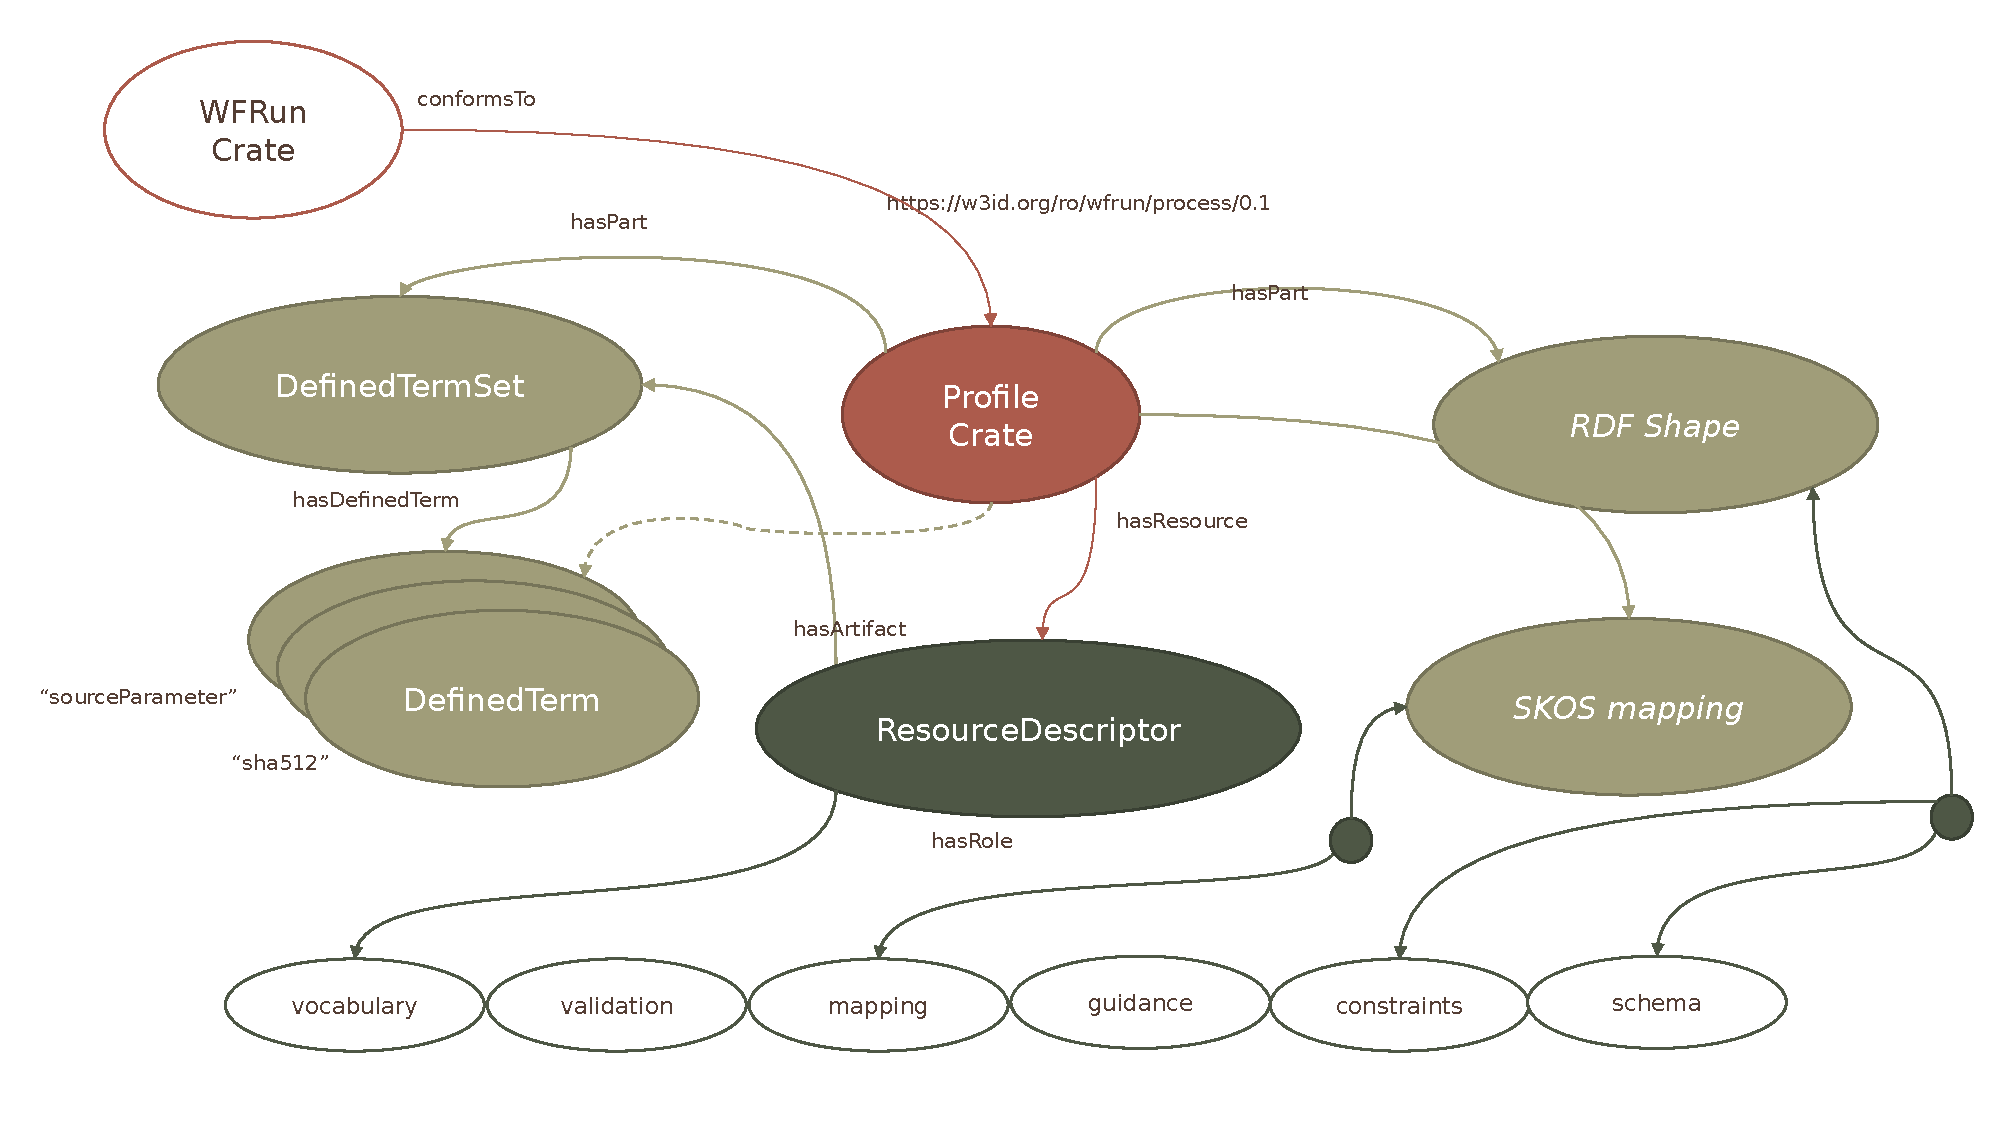
\includegraphics[width=\textwidth]{figures/ch09/profile-crate.pdf}
      \caption[Example of Profile Crate]{\textbf{Example of Profile Crate for Workflow Run Crate}. 
      An RO-Crate \emph{WFRun Crate} declares conformance with a given RO-Crate profile. 
      Resolving the profile URI retrieves the \emph{Profile Crate}, which parts include an \emph{RDF Shape}, an \emph{SKOS mapping} and a \emph{DefinedTermSet}. 
      By using the indirection of \emph{ResourceDescriptor} from the Profiles Vocabulary \cite{dx-prof}, the roles of each of these artefacts are defined, e.g. \emph{constraints}. 
      The embedded \emph{vocabulary} as a \emph{DefinedTermSet} defines ad-hoc terms like \emph{sourceParameter} used by the Workflow Run Crate\footnotemark~ profile \cite{workflow-run-crate}.
      }
    \label{ch61:fig:profilecrate}
  \end{figure}
\footnotetext{\url{https://w3id.org/ro/wfrun/process/0.2}}

While profiles are at first lightweight indicators of common conventions for a class of crates (which may be implicit or explicit), they can be gradually formalized in a \emph{eat own dogfood} way through another RO-Crate, optionally taking advantage of existing Semantic Web technology that can enable for instance strict validation of domain-specific RO-Crates.


\subsubsection{One vocabulary is not enough, but one profile may suffice}
\label{ch61:oneprofile}

RO-Crate relies heavily on \cite{schema.org} as its main vocabulary, but as highlighted in section \vref{ch5:futurework} and \vref{ch61:profiles}, domain-specific usage will eventually need to define their own terms in order to be specific enough for their use cases. However, we have found it is important to ensure a developer-friendly approach when specifying such profiles for RO-Crate -- earlier work on \footurl{https://www.researchobject.org/ro-crate/1.1/appendix/jsonld.html\#adding-new-or-ad-hoc-vocabulary-terms}{ad-hoc terms} in RO-Crate used a simple CSV approach to be added to the \footurl{https://github.com/ResearchObject/ro-terms}{ro-terms} namespace.  

As with other aspects of RO-Crate, there is a gradual approach towards Linked Data practices. While conventional wisdom in Semantic Web would be to sit down and make your own ontology following design patterns \cite{Blomquist 2009,Poveda 2010} and best practices for deployment \cite{Matentzoglu 2022}, in RO-Crate philosophy that would be more of a last resort. The middle of the ground is therefore adding the ad-hoc vocabulary directly to the profile crate, as shown in figure \vref{ch61:fig:profilecrate}. In this approach a single profile URI can, through Linked Data and Signposting, play the role of:

\begin{itemize}
  \item Human-readable documentation of conventions (negotiated to HTML preview)
  \item List of software and repositories the profile is intended for
  \item List of additional schema.org types and properties utillised by the profile
  \item Indication of which content is expected in the crate (e.g. a Workflow)
  \item Validation of a manifest conforming to the profile
  \item Vocabulary definitions of additional terms
  \item JSON-LD context which namespaces the additional terms  (as any JSON-LD document can also be a JSON-LD context \cite{w3-json-ld})
\end{itemize}

It should be reasonable to expect developers able to make RO-Crates with their own additional terms to also be able to make a lightweight Profile Crate once those terms have stabilised. Developers with deeper familiarity with Semantic Web technologies can expand the profile capabilities to use existing ontology methodologies, in which case it would be preferrable to aggregate separate semantic artefacts from the Profile Crate rather than embedding them in the RO-Crate Metadata File.

In the FAIR-IMPACT project we are evaluating if the Profile Crate approach is also suitable for FAIR publishing of semantic artefacts themselves, e.g. ontologies and mappings. This is an attractive proposal because such artefacts are also becoming multifaceted, with multiple formats and profiles (e.g. an ontology expressed with OWL2 RL in RDF Turtle syntax), documentation and similar attribution and provenance challenges that RO-Crate resolves.

\subsection{Future RO-Crate directions}
\label{ch61:rocratefuture}
In this section we consider future directions for RO-Crate and ongoing RO-Crate adaptations not covered by section \ref{ch5:packaging-research-artefacts-with-ro-crate}.


\subsubsection{User applications are needed for researchers to generate FAIR Research Objects}
\label{ch61:applications}

RO-Crate and its best practices can be considered a type of \emph{middleware} used by application developers to capture and transmit metadata and relate data files that together form some tangible unit (a \emph{Research Object} \cite{Bechhofer 2013}). While RO-Crate have already been implemented by several repositories and applications such as workflow systems, it is important to also consider the role of user applications in order to increase adoptation of FAIR research objects by scholars in general.

Futher work by the RO-Crate community has created more user-fronting tools such as \footurl{https://github.com/oeg-upm/ya2ro}{ya2ro}, which given metadata and identifier in a YAML\footnote{
  YAML is a file format with the same data model as JSON, but with a more readable syntax, e.g. using indentation instead of quoted strings.  \url{https://yaml.org/}} 
file can retrieve contextual metadata from ORCID, GitHub and DOI registries and build and publish a completed RO-Crate \cite{ya2ro}.   
While this technology still requires some understanding of editing, it is intended to be more approachable to data scientists and for use with simple Web publishing platforms like \footurl{https://pages.github.com/}{GitHub Pages}. The GitHub Action \footurl{https://github.com/marketplace/actions/ro-crate-preview}{ro-crate-preview} also automate HTML preview generation of crates on GitHub Pages.

The repository \footurl{https://www.rohub.org/}{ROHub} \cite{ch5-48} has recently added RO-Crate import and export \cite{Fouilloux 2023}, and provides both a browseable repository for publishing crates, but also interactive and collaborative editing of its metadata. 
In this use case, RO-Crate plays the role as an exchange and archiving format, as the hub stores the crates in general-purpose repositories Zenodo and B2Share which do not have the facility to keep the granular metadata expressed within the RO-Crate metadata file. As detailed in \cite{Fouilloux 2023}, a series of templates assist users in creating research objects with particular content and annotations. 

The \footurl{https://schema.org/docs/schemas.html}{Crate-O} tool has been developed by Language Data Commons of Australia \footurl{https://ldaca.edu.au/}{(LDaCA)} as a general-purpose RO-Crate editor and successor to Describo \cite{ch5-78} and Describo Online \cite{ch5-77}. 
This tool can describe any folder and resources from the Web as an RO-Crate, supporting any schema.org type and property, pluggable with any rdfs vocabularies \cite{w3-rdf-schema}. 
Notably this tool is also intended for creation of such vocabularies, and is thus a lightweight user interface for building a Profile Crate (section \vref{ch61:profiles}) using Schema.org style Schemas\footnote{
  It is notable that schema.org's own vocabulary definition use rdfs directly for Linked Data interoperability, 
  rather than its own \url{http://schema.org/Class}, \url{http://schema.org/Property}, or the SKOS-like \url{http://schema.org/DefinedTerm}. 
  On property definitions, SoSS use \url{http://schema.org/domainIncludes} and \url{http://schema.org/rangeIncludes} to avoid union classes for alternative domain/range types, which can clutter OWL/RDFS equivalent properties.} 
\footurl{https://schema.org/docs/schemas.html}{(SoSS)}.


\subsubsection{Executable paper using RO-Crate}
\label{ch61:livepublication}

\footurl{https://livepublication.github.io/LP_Pub_LID/}{LivePublication} \cite{Ellerm 2023} is a proof of concept of an \emph{executable paper}, which interactive visualization and statistical calculations can be regenerated on the fly taking into consideration data sources updated after the paper's publication date. A \footurl{https://livepublication.github.io/LP_Pub_OrchestrationCrate/}{corresponding RO-Crate} is the mechanism to enable this execution on the Globus infrastructure through individual RO-Crates and containers for each computable element of the paper.

This novel approach shows how it is possible to use RO-Crate as an machine-actionable object, which do not rely on bundling an underlying workflow representation in an existing workflow language.  

\subsubsection{Web-based FDOs can use RO-Crate for its metadata}
\label{ch61:webfdo}

Section \vref{ch4:lightweight-fdo} argues that many of the FDO requirements \cite{fdo-RequirementSpec} for metadata can be implemented as \emph{RO-Crate FDOs} (section \vref{ch8:fair-packaging-of-researchworkflow-objects-with-ro-crate}), with FAIR Signposting \cite{vandesompel2015,Van de Sompel 2022} assisting navigation from persistent identifiers, and the RO-Crate containing the metadata. 

This approach was first implemented in the repository WorkflowHub \cite{Goble 2021,wittenburgFAIRDigitalObject2022b}, and in the FDO Forum \cite{Van de Sompel 2023} suggests RO-Crate with Signposting as a modern update to his OAI-ORE\footnote{OAI-ORE was also used by earlier Research Object approaches \cite{Belhajjame 2015,ch5-111} to capture the aggregation aspect of ROs.} approach from 2008 \cite{ORESpecificationAbstract}.  
RO-Crate FDOs are being further developed within the Horizon Europe projects \footurl{https://eurosciencegateway.eu/}{EuroScienceGateway} \cite{10.5281/zenodo.7152762} and \footurl{https://fair-impact.eu/}{FAIR-IMPACT} \cite{10.5281/zenodo.7157647}.

RO-Crate FDOs complements the findings of section \vref{ch61:signposting}, in that RO-Crate provides FDO with a generic metadata framework and a serialization that can work both for FDOs on the Web and with legacy Handle/DOIP approaches --  this metadata role for RO-Crate in the FDO ecosystem is also highlighted by \cite{Wittenburg 2023b}.

Some extra considerations is rightly needed on identifiers to reduce relative paths challenges with  RO-Crate FDOs -- for this purpose, the next specification \cite{rocrate1.2} introduce a distinction between an \footurl{https://www.researchobject.org/ro-crate/1.2-DRAFT/structure.html\#attached-ro-crate}{attached RO-Crate} (\emph{has some root directory containing other files referenced by relative paths, possibly archived in a ZIP or exposed on the Web}) and a \footurl{https://www.researchobject.org/ro-crate/1.2-DRAFT/structure.html\#detached-ro-crate}{detached RO-Crate} (\emph{no defined root directory, all references are absolute}). 
This \emph{detached} style is suitable for an FDO architecture, even for use within APIs which do not lend themselves to relative path references (such as DOIP-over-HTTP \cite{DOIPAPIHTTPa}).
RO-Crate 1.2 also define methods for \footurl{https://www.researchobject.org/ro-crate/1.2-DRAFT/appendix/relative-uris.html}{converting between attached/detached} crates using standard JSON-LD tooling, showing another advantage of using Linked Data as basis for RO-Crate. 


\paragraph{How FAIR are RO-Crates?}
\label{ch61:fair-crates}

FAIROs \cite{FAIROs} is a framework for calculating a ``FAIRness'' score for research objects. For RO-Crate evaluation this puts additional requirements on the use of persistent identifier for the RO-Crate, and that the core metadata of the crate (e.g. licensing) is provided. These aspects are important for ensuring FDO machine actionability of RO-Crates.


\subsubsection{RO-Crate can capture collections of digital objects}
\label{ch61:collections}

RO-Crate has also been proposed as a generic mechanism for FDO Collections \cite{fdo-collections}, as an aggregator of FDOs by their PIDs. Such collections add a similar challenge in FDO as in Linked Data, in that clients may need to resolve an excessive number of persistent identifiers (see section \vref{ch20:avoid-lots-of-requests}) to FDOs which may be of different semantic types. 
Using a detached RO-Crate for such collections, the bibliographic metadata of each PID can be directly embedded and normalized to a single vocabulary, reducing client needs for recursive queries and type mappings. 
 
Work on building large data citations as a ``reliquary'' -- a \emph{container of persistent identifiers (PIDs)} \cite{Buck 2022} -- started from the earth science domain with AGU's \footurl{https://data.agu.org/DataCitationCoP/}{Data Citation Community of Practice} and continues in RDA's \footurl{https://www.rd-alliance.org/groups/complex-citations-working-group}{Complex Citation Working Group}. In this approach RO-Crate is being considered as a promising implementation to capture large number of citations along with minimal metadata, including licensing and attribution. Here a main motivation is to avoid excessive lists of data citations for scholarly publications following processing of aggregated datasets from repositories such as GBIF \cite{ch8-7}, while still propagating each dataset's FAIR metadata (as required by the Creative Commons Attribution licence) through the indirection of a collection. There is a potential overlap with workflow run provenance, although a workflow is not required by reliquaries.


\subsubsection{RO-Crate in data lakes}
\label{ch61:datalakes}

Knowledge Enhanced Digital Objects \footurl{https://github.com/luoyu357/KEDODataLake}{(KEOD)} \cite{Luo 2022} is an experimental approach of building a data lake using a combination of knowledge graphs, RO-Crate and PID records \cite{Luo 2023}. This is effectively an FDO implementation: A KEDO PID is a Handle that identifies a KEDO Object, described using a KEDO RO-Crate. This crate again has \emph{internal RO-Crate}s as parts, which records a combination of \emph{Features} and \emph{Insights}. The distinction is that features are mainly fixed at digital object creation and considered directly describing the object's nature, while insights can be discovered later from further processing and linkage. This approach solves a mutability problem in FDOs, as the KEOD system only allows insights to be added along with provenance that connect PIDs when KEDOs evolve. Files in a KEDO RO-Crate are stored locally, and each recorded with a Handle PID within the crate.

This KEOD setup of multiple graphs forming a single knowledge unit can be considered analoguous to nanopublications \cite{Kuhn 2021} but for FDOs. Indeed using nanopublication to capture FDOs of digital twins has also been proposed \cite{10.3389/data.2022.883341}, that however use a different distributed architecture where the PIDs for nanopublications are generated by cryptographically hashing their content \cite{Kuhn 2021}.


\subsubsection{Distributed FAIR Digital Objects using Blockchain}
\label{ch61:dpid}

The \footurl{https://docs.desci.com/}{DeSci Nodes} system has been developed by the \footurl{https://www.descifoundation.org/}{DeSci foundation}, where \footurl{https://www.dpid.org/}{dPID} (distibuted Persistent Identifier) act  as an overlay of the Interplanetary File System (IPFS) \cite{Trautwein 2022}. Users can interact with the DeSci platform for building and publishing Research Objects, and the \footurl{https://docs.desci.com/learn/open-state-repository/metadata}{DeSci metadata} are exposed as a \footurl{https://www.researchobject.org/ro-crate/1.2-DRAFT/structure.html\#detached-ro-crate}{detached RO-Crate} with IPFS references (see \footurl{https://beta.dpid.org/46?jsonld}{example dPID 46}).

This is a novel FAIR Digital Object implementation that challenges both the traditional centralised FDO approach using the Handle system, as well as the mostly Web-based RO-Crate ecosystem covered in section \vref{ch5:packaging-research-artefacts-with-ro-crate}. The use of detached crates has also been \footurl{https://www.researchobject.org/ro-crate/in-use/LDaCA.html}{Language Data Commons of Australia Program}, where RO-Crate is part of navigating API resources, rather than a standalone publication on the Web. In both of these approaches, additional FDO measures such as using persistent identifiers and validation against profiles become important. 




\subsection{Workflow}
\label{ch61:workflow}

Chapter \vref{chapter:workflows} explored in depth different ways in which FAIR Digital Objects and RO-Crate are applied to computational workflows. 

\subsubsection{Workflows as FAIR digital objects}
\label{ch61:workflowfdo}

We have previously proposed the concept of \emph{FAIR Computational Workflows} \cite{Goble 2020}. 
That work expands on the well-established motivations for using scientific workflow systems \cite{ch6-4,Atkinson 2017}, such as supporting Automation, Scalable execution, Abstraction, and Provenance \cite{Ludascher 2016}, and highlights that workflows themselves benefit from and contribute to FAIR data, for instance providing metadata for describing workflow outputs. 
In addition workflow themselves can be considered digital objects that should be shared as a reproducible computational method.

Applying the FAIR principles for workflows in practice has however revealed additional challenges, such as lack of clarify of what constitutes a \emph{workflow} as opposed to FAIR Research Software in general \cite{Katz 2021b}, or reduced reusability when the workflow requires unwritten, human-centric operations between computational steps (e.g. trivial file column manipulations) \cite{wilkinsonWorkflowsWhenParts2022b}. 

In developing the repository \footurl{https://workflowhub.eu/}{WorkflowHub} \cite{Goble 2021} we emphasised the importance of preserving and publishing not just executable workflow definitions, 
but their structured descriptions independent of workflow formats as well as further references to external sources, software required (including the workflow engine).
For this we developed the Workflow RO-Crate Profile \cite{Bacall 2022}, which became a foundational format for more specific workflow execution profiles (section \vref{ch54:wrroc}).

One aspect that makes workflow management systems different from research software in general, is that the they frequently encourage modularization, in that the composition of steps also can reflect the analytical process that is intended by the scientists.
Mature workflow systems like Galaxy \cite{Galaxy 2022} provide a large collection of re-usable components that wrap underlying command line tools and make them interoperable without manual adjustments. 
In CWL  \cite{Crusoe 2022}, tool definitions include not just execution details, but also structured input/output definitions, allowing them to be reused and combined in multiple workflows.

Section \vref{ch6:making-canonical-workflow-building-blocks-interoperable-across-workflow-languages} explored how such building blocks can themselves be considered FAIR digital objects. These assist workflow systems in propagating rich metadata about tools and their analytical purpose, but also allows building blocks to be reused across workflow systems. This in effect means that a \emph{canonical workflow} \emph{ch8-27} can be implemented in different workflow languages, each executing the same \emph{canonical steps} in the same way. Given that FAIR Digital Objects emphasize machine-actionability, and we can consider workflows as FDOs, it is important to have the ability not just to reliably re-execute a workflow, but even re-use its constituent steps. 


\subsubsection{Using and building FDOs from workflows}
\label{ch61:buildingfdo}

Section \vref{ch8:the-specimen-data-refinery} 


\subsubsection{Provenance of workflow runs}
\label{ch61:provenance}

\cite{workflow-run-crate}

Section \vref{ch54:wrroc}


\subsubsection{Combining multiple FDO types in workflows?}
\label{ch61:combining}

\cite{Wittenburg 2023a}

\textbf{TODO}: Summarize/discuss 
From \vref{ch8:the-specimen-data-refinery}:

  \begin{quotation}
  Both kinds of FDO are essential.
  They complement one another to support
  implementation of the FAIR principles, especially the interoperable and
  reusable principles by making workflows self-documenting.
  This renders
  automated whole processes (or fragments thereof) for digitizing and
  extending natural history specimens' data as FAIR without adding
  additional load to the researchers that stand to benefit most from that
  \cite{ch8-27}.
  Each FDO type originates from different Research
  Infrastructures (ELIXIR, DiSSCo) with different implementation
  frameworks.
  Yet, they interoperate effectively due to their clear roles,
  common conceptual model and separation of concerns.


  openDS FDOs have their heritage in distributed digital object services
  \cite{Kahn 2006} and are implemented through Digital Object Architecture (DOA)
  \cite{ch8-62} with Digital Object Interface Protocol (DOIP) \cite{DONA 2018}, Digital
  Object Identifier Resolution Protocol (DO-IRP) \cite{rfc3652}, and
  recommendations of the Research Data Alliance \cite{ch8-65}.
  Serialized as
  JSON, they are machine-actionable and compatible with established
  protocols of the World Wide Web.

  RO-Crates are native to the World Wide Web, based on established web
  protocols, machine-readable metadata using Linked Data Platform methods
  \cite{ch8-66}, JSON-LD and Schema.org \cite{Bechhofer 2013}, and community-accepted
  packaging mechanisms such as BagIt.
  This makes RO-Crates straightforward
  to incorporate into pre-existing platforms such as Galaxy and data
  repositories such as Zenodo and DataVerse.

  Both kinds of FDO use Persistent identifiers (PID), allowing instances
  to be both uniquely identified and their location to be determined;
  RO-Crates, as web natives, use URIs whereas openDS, as DOA objects, use
  Handle PIDs.
  Instances of both kinds are described by metadata and
  contain or reference data.

  RO-Crates are self-describing using a metadata file and use
  openly-extensible profiles to type the Crates (profile-typing) to set
  out expectations for their metadata and content. openDS uses an
  object-oriented object typing and instance approach to define the
  structure and content of data/metadata.
  Complex object types are
  constructed from basic types, an extension-section basic type.
  Both
  approaches seek to avoid locking objects into repository silos, ensuring
  that FDO instances can be interpreted outside of the contexts in which
  they were originally created/stored.

  Structurally and semantically openDS FDOs and RO-Crate FDOs are
  potentially isomorphic, although at different granularity levels.
  Their
  main difference is in method calling.
  As a DOA object, openDS would
  expect to respond to type-specific method calls if these were
  implemented.
  RO-Crates delegate actionability to applications that
  interpret their self-describing profile.

  Within the SDR the two kinds of FDO fulfill distinct and interlocking
  roles for data (openDS) and self-documented method (RO-Crate) so their
  different forms is not an issue.
  In future there may be a need to map
  and convert between the approaches (e.g., for reconstructing past
  processing), which would be assisted by the common FDO conceptual model
  \cite{bonino2019}.

\end{quotation}


\subsubsection{FDOs can be built incrementally with workflows}
\label{ch61:incremental}
\textbf{TODO}: Summarize/discuss 
From \vref{ch7:incrementally-building-fair-digital-objects-with-specimen-data-refinery-workflows}:

\begin{quotation}
  SDR is an example of machine-assisted construction of FDOs, which
  highlight the needs for intermediate digital objects that are not yet
  FDO compliant.
  The passing of such ``local FDOs'' is beneficial not just
  for efficiency and visual inspection, but also to simplify workflow
  composition of canonical workflow building blocks.
  At the same time we
  see that it is insufficient to only pass FDOs as JSON objects, as they
  also have references to other data such as images, which should not need
  to be re-downloaded.

  Further work will investigate the use of RO-Crate as a wrapper of
  partial FDOs, but this needs to be coupled with more flexible FDO types
  as profiles, in order to restrict ``impossible'' ordering of steps
  depending on particular inner FDO fragments.
  A distinction needs to be
  made between open digital specimens that are in ``draft'' state and
  those that can be pushed to DiSSCo registries.

  We are experimenting with changing the SDR components into Canonical
  Workflow Building Blocks \cite{Soiland-Reyes 2022b}
  (\vref{ch6:making-canonical-workflow-building-blocks-interoperable-across-workflow-languages}) 
  using the Common Workflow Language \cite{Crusoe 2022}.
  This gives
  flexibility to scalably execute SDR workflows on different compute
  backends such as HPC or local cluster, without the additional setup of
  Galaxy servers.
\end{quotation}

\section{Conclusions}

\subsection{Main findings}

From research question \textbf{RQ1} (section \vref{intro:rq1}) I asked if the FAIR Digital Object (FDO) concept was realisable using existing Web technology, which was explored by chapters \ref{chapter:background} and \ref{chapter:fdo} and discussed in section \ref{ch61:discuss}. The brief conclusion is that Web approaches can practically achieve FDO goals, by combining existing standards in a normated way. However FAIR practitioners cannot simply equate Semantic Web with FDO, but need to also ensure sufficient constraints to guarantee navigational machine-actionability, balanced against developer usability and extensibility. 

For research question \textbf{RQ2} (section \vref{intro:rq2}) I endevour further on the challenge mentioned above: Chapter \ref{chapter:ro-crate} introduced \emph{RO-Crate} as such a pragmatic and normative approach that has been implemented by multiple open source developers for a wide range of applications. As discussed in section \ref{ch61:discuss}, to build a reliable and extensible FDO ecosystem, the lightweight recommendations of RO-Crate needs to be combined with community-developed profiles which provide validation and tailored user interfaces.

In answer to the final research question \textbf{RQ3} (section \vref{intro:rq3}), chapter \ref{chapter:workflows} covered different aspects, by proposing research software wrapped as canonical workflow building blocks, incrementally building FDOs from a workflow system, and recording workflow execution provenance. All of these have in common that they are implemented using RO-Crate and compatible with the other approaches from chapter \ref{chapter:ro-crate}, e.g. for visualisation and editing. For workflow provenance, section \vref{ch54:wrroc} introduced the Workflow Run Crate profiles (WRROC). These were implemented by six different workflow systems, with maturing tooling and practical use cases that showcase how different developers (many not familiar with Semantic Web technologies) can adopt an interoperable approach to FDOs using pragmatic guidance to Linked Data.




\appendix
\fancyhead[RE]{Appendix \thechapter}

\chapter{Acknowledgements}
\label{chapter:acknowledgements}
\label{ch11:acknowledgements}

\hypertarget{personal-acknowledgements}{%
\section{Personal acknowledgements}\label{personal-acknowledgements}}

% family
% Paul
% Carole
% colleagues
% Sarven
% Meznah
% Bijan
% UCU

\hypertarget{community-acknowledgements}{%
\section{Community acknowledgements}\label{community-acknowledgements}}

\subsection{RO-Crate Community}\label{communitylist}
\label{ro-crate-community}

I am forever grateful for all the wonderful discussions, technical contributrions and long-lasting friendships formed in the RO-Crate community since its early inception \cite{OCarragain 2019} at Workshop on Research Objects \footurl{https://www.researchobject.org/ro2018/}{(RO2018)}. Without you there would not have been any RO-Crate!

I would particularly like to thank Peter Sefton, without which co-chairing, enthusiasm and pragmatism I would easily had got lost the weeds.  I am forever in debt to Eoghan Ó Carragáin who managed to get me and Peter to agree even on the trickiest issues, and led the community through its formative years.

I want to thank Simone Leo, which persistent work and leadership on \footurl{https://w3id.org/ro/wfrun/}{Workflow Run Crate} and the RO-Crate Python library \cite{ro-crate-py} has shown that RO-Crate works in practice even for detailed provenance. 

I am very grateful to Daniel Garijo, with whom I have enjoyed many insightful discussions and idea developments for more than a decade (since the early days of Research Objects), not to mention his many invaluable and constructive edits to manuscripts and specifications.

RO-Crate is standing on the shoulders of giants, and I would like to thank the whole Research Object community \cite{goble-ro2018} for persisting on the early RO ideas \cite{ch5-93, Bechhofer 2013}. I have particular fond memories of whiteboard sessions with Sean Bechhofer, Khalid Belhajjame, Paolo Missier, David De Roure, and Kevin Page in the productive \footurl{https://s11.no/2020/archive/wf4ever/}{Wf4Ever project} that laid the foundation for what is now RO-Crate.


As of 2023-06-15, the \emph{RO-Crate} \footurl{https://www.researchobject.org/ro-crate/community.html}{Community members} are:

\begin{longtable}{lll}
  Peter Sefton & \url{https://orcid.org/0000-0002-3545-944X} & (co-chair) 
\\
  Stian Soiland-Reyes & \url{https://orcid.org/0000-0001-9842-9718} & (co-chair) 
\\
  Eoghan Ó Carragáin & \url{https://orcid.org/0000-0001-8131-2150} & (emeritus chair) 
\\
  Oscar Corcho & \url{https://orcid.org/0000-0002-9260-0753}
\\
  Daniel Garijo & \url{https://orcid.org/0000-0003-0454-7145}
\\
  Raul Palma & \url{https://orcid.org/0000-0003-4289-4922}
\\
  Frederik Coppens & \url{https://orcid.org/0000-0001-6565-5145}
\\
  Carole Goble & \url{https://orcid.org/0000-0003-1219-2137}
\\
  José María Fernández & \url{https://orcid.org/0000-0002-4806-5140}
\\
  Kyle Chard & \url{https://orcid.org/0000-0002-7370-4805}
\\
  Jose Manuel Gomez-Perez & \url{https://orcid.org/0000-0002-5491-6431}
\\
  Michael R Crusoe & \url{https://orcid.org/0000-0002-2961-9670}
\\
  Ignacio Eguinoa & \url{https://orcid.org/0000-0002-6190-122X}
\\
  Nick Juty & \url{https://orcid.org/0000-0002-2036-8350}
\\
  Kristi Holmes & \url{https://orcid.org/0000-0001-8420-5254}
\\
  Jason A. Clark & \url{https://orcid.org/0000-0002-3588-6257}
\\
  Salvador Capella-Gutierrez & \url{https://orcid.org/0000-0002-0309-604X}
\\
  Alasdair J. G. Gray & \url{https://orcid.org/0000-0002-5711-4872}
\\
  Stuart Owen & \url{https://orcid.org/0000-0003-2130-0865}
\\
  Alan R Williams & \url{https://orcid.org/0000-0003-3156-2105}
\\
  Giacomo Tartari & \url{https://orcid.org/0000-0003-1130-2154}
\\
  Finn Bacall & \url{https://orcid.org/0000-0002-0048-3300}
\\
  Thomas Thelen & \url{https://orcid.org/0000-0002-1756-2128}
\\
  Hervé Ménager & \url{https://orcid.org/0000-0002-7552-1009}
\\
  Laura Rodríguez-Navas & \url{https://orcid.org/0000-0003-4929-1219}
\\
  Paul Walk & \url{https://orcid.org/0000-0003-1541-5631}
\\
  brandon whitehead & \url{https://orcid.org/0000-0002-0337-8610}
\\
  Mark Wilkinson & \url{https://orcid.org/0000-0001-6960-357X}
\\
  Paul Groth & \url{https://orcid.org/0000-0003-0183-6910}
\\
  Erich Bremer & \url{https://orcid.org/0000-0003-0223-1059}
\\
  LJ Garcia Castro & \url{https://orcid.org/0000-0003-3986-0510}
\\
  Karl Sebby & \url{https://orcid.org/0000-0001-6022-9825}
\\
  Alexander Kanitz & \url{https://orcid.org/0000-0002-3468-0652}
\\
  Ana Trisovic & \url{https://orcid.org/0000-0003-1991-0533}
\\
  Gavin Kennedy & \url{https://orcid.org/0000-0003-3910-0474}
\\
  Mark Graves & \url{https://orcid.org/0000-0003-3486-8193}
\\
  Jasper Koehorst & \url{https://orcid.org/0000-0001-8172-8981}
\\
  Simone Leo & \url{https://orcid.org/0000-0001-8271-5429}
\\
  Marc Portier & \url{https://orcid.org/0000-0002-9648-6484}
\\
  Paul Brack & \url{https://orcid.org/0000-0002-5432-2748}
\\
  Milan Ojsteršek & \url{https://orcid.org/0000-0003-1743-8300}
\\
  Bert Droesbeke & \url{https://orcid.org/0000-0003-0522-5674}
\\
  Chenxu Niu & \url{https://orcid.org/0000-0002-2142-1731}
\\
  Kosuke Tanabe & \url{https://orcid.org/0000-0002-9986-7223}
\\
  Tomasz Miksa & \url{https://orcid.org/0000-0002-4929-7875}
\\
  Marco La Rosa & \url{https://orcid.org/0000-0001-5383-6993}
\\
  Cedric Decruw & \url{https://orcid.org/0000-0001-6387-5988}
\\
  Andreas Czerniak & \url{https://orcid.org/0000-0003-3883-4169}
\\
  Jeremy Jay & \url{https://orcid.org/0000-0002-5761-7533}
\\
  Sergio Serra & \url{https://orcid.org/0000-0002-0792-8157}
\\
  Ronald Siebes & \url{https://orcid.org/0000-0001-8772-7904}
\\
  Shaun de Witt & \url{https://orcid.org/0000-0003-4196-3658}
\\
  Shady El Damaty & \url{https://orcid.org/0000-0002-2318-4477}
\\
  Douglas Lowe & \url{https://orcid.org/0000-0002-1248-3594}
\\
  Xuanqi Li & \url{https://orcid.org/0000-0003-1498-6205}
\\
  Sveinung Gundersen & \url{https://orcid.org/0000-0001-9888-7954}
\\
  Muhammad Radifar & \url{https://orcid.org/0000-0001-9156-9478}
\\
  Rudolf Wittner & \url{https://orcid.org/0000-0002-0003-2024}
\\
  Oliver Woolland & \url{https://orcid.org/0000-0002-4565-9760}
\\
  Paul De Geest & \url{https://orcid.org/0000-0002-8940-4946}
\\
  Douglas Fils & \url{https://orcid.org/0000-0002-2257-9127}
\\
  Florian Wetzels & \url{https://orcid.org/0000-0002-5526-7138}
\\
  Raül Sirvent & \url{https://orcid.org/0000-0003-0606-2512}
\\
  Abigail Miller & \url{https://orcid.org/0000-0001-9228-2882}
\\
  Jake Emerson & \url{https://orcid.org/0000-0003-0617-9219}
\\
  Davide Fucci & \url{https://orcid.org/0000-0002-0679-4361}
\\
  Bruno P. Kinoshita & \url{https://orcid.org/0000-0001-8250-4074}
\\
  Maciek Bąk & \url{https://orcid.org/0000-0003-1361-7301}  
\\
  Jens Hollunder & \url{https://orcid.org/0000-0003-3234-6762}
\end{longtable}


\subsection{ELIXIR}
\footurl{https://elixir-europe.org/}{ELIXIR Europe}

% Frederik, Ignacio, JM, Laura, Niklas
% Leyla Jael	Castro

\subsection{CWL Community}

% MrC, Peter, Hervé, leadership team

\subsection{FDO Community}

% PeterW, Luiz	Bonino, Maggie	Hellström, Rainer	Stotzka

\subsection{FAIR Community}

% Herbert
% Mark, Daniel

\subsection{Other communities}

* BioComputeObject
* WCI 
* ISO provenance % , Rudolf
* RDA
* PROV 


\newpage
\section{My funding}

My work presented in this thesis has been undertaken during 
several research projects at The University of Manchester, 
which funding is acknowledged below:

\begin{longtable}{rlll}
\multicolumn{3}{l}{\textbf{European Commission programme Horizon H2020}} 
\\
H2020-INFRAEDI-02-2018 & 
\footurl{https://doi.org/10.3030/823830}{823830} & 
\footurl{https://bioexcel.eu/}{BioExcel-2} & 
\\
H2020-INFRAEOSC-2018-2 & 
\footurl{https://doi.org/10.3030/824087}{824087} & 
\footurl{https://www.eosc-life.eu/}{EOSC-Life} & 
\\
H2020-INFRAIA-2017-1-two-stage & 
\footurl{https://doi.org/10.3030/730976}{730976} & 
\footurl{https://ibisba.eu/}{IBISBA 1.0}
\\
H2020-INFRAIA-2018-1 & 
\footurl{https://doi.org/10.3030/823827}{823827} & 
\footurl{https://www.synthesys.info/}{SyntheSys+}
\\
\\
\multicolumn{3}{l}{\textbf{European Commission programme Horizon Europe}} & \textbf{UKRI}\footnote{UK Research and Innovation under the UK government’s  \emph{Horizon Europe funding guarantee}} 
\\
HORIZON-INFRA-2021-EMERGENCY-01 & 
\footurl{https://doi.org/10.3030/101046203}{101046203} & 
\footurl{https://by-covid.eu/}{BY-COVID}
\\
HORIZON-INFRA-2021-EOSC-01 & 
\footurl{https://doi.org/10.3030/101057388}{101057388} & 
\footurl{http://eurosciencegateway.eu/}{EuroScienceGateway} & 
\footurl{https://gtr.ukri.org/projects?ref=10038963}{10038963}
\\
HORIZON-INFRA-2021-TECH-01 & 
\footurl{https://doi.org/10.3030/101057437}{101057437} & 
\footurl{https://biodt.eu/}{BioDT} & 
\footurl{https://gtr.ukri.org/projects?ref=10038930}{10038930}
\\
HORIZON-INFRA-2021-EOSC-01-05 & 
\footurl{https://doi.org/10.3030/101057344}{101057344} & 
\footurl{https://fair-impact.eu/}{FAIR-IMPACT} & 
\footurl{https://gtr.ukri.org/projects?ref=10038992}{10038992} 
\\

\\
\multicolumn{3}{l}{\textbf{UK Research and Innovation (UKRI)}} \\
MRC / \footurl{https://dareuk.org.uk/driver-project-tre-fx/}{DARE-UK}\footnote{Call: \textit{Inform design of cross-council trusted research environments}} & 
	&
	\footurl{https://trefx.uk/}{TRE-FX} &
\footurl{https://gtr.ukri.org/projects?ref=MC_PC_23007}{MC\_PC\_23007}  

\end{longtable}

\section{Funding and acknowledgements for co-authored chapters}

%%

\subsection{Acknowledgements for \textit{Evaluating FAIR Digital Object and Linked Data as distributed object systems}}\label{ch11:fdo}

Setions \vref{ch3:background} and \vref{ch3:evaluating-fdo-ld} are adapted from an arXiv preprint submitted to PeerJ CS for peer review.

\subsubsection*{Published As}

Stian Soiland-Reyes, Carole Goble, Paul Groth (2023):\\
\textbf{Evaluating FAIR Digital Object and Linked Data as distributed object systems}.\\
\emph{arXiv} 2306.07436 [cs.DC] \\
\url{https://doi.org/10.48550/arXiv.2306.07436}

An \footurl{https://w3id.org/ro/doi/10.5281/zenodo.8075229}{RO-Crate for
this article} is archived at
\url{https://doi.org/10.5281/zenodo.8075229}

\subsubsection*{Acknowledgements}

We would like to acknowledge the \footurl{https://fairdo.org/}{FAIR Digital Object Forum} community and working groups, where SSR and CG are members.

Views and opinions expressed in this work are those of the authors only and do not necessarily reflect those of the funded projects, FAIR Digital Object Forum, European Union nor the European Commission.

\subsubsection*{License and modifications}

\begin{itemize}
\tightlist
\item
  \textbf{License}: Creative Commons Attribution License
  \href{https://spdx.org/licenses/CC-BY-4.0}{(CC BY 4.0)}.
\item
  \textbf{Modifications}: Minor LaTeX changes; references in s11 house style; 
  citations merged and renumbered; 
  funding and references moved to separate chapters. Background moved to separate chapter, 
  added figures \ref{ch3:fig:fdo}, \ref{ch3:fig:jsonld} and listing \ref{ch3:triples}.
\end{itemize}

\subsubsection*{Funding}

This work was funded by the European Union programmes \emph{Horizon 2020} under grant agreements H2020-INFRAEDI-02-2018 823830 (BioExcel-2), H2020-INFRAEOSC-2018-2 824087 (EOSC-Life) and \emph{Horizon Europe} under grant agreements HORIZON-INFRA-2021-EMERGENCY-01 101046203 (BY-COVID), HORIZON-INFRA-2021-EOSC-01 101057388 (EuroScienceGateway), HORIZON-INFRA-2021-EOSC-01-05 101057344 (FAIR-IMPACT), HORIZON-INFRA-2021-TECH-01 101057437 (BioDT), HORIZON-CL4-2021-HUMAN-01-01 101070305 (ENEXA); and by UK Research and Innovation (UKRI) under the UK government’s \emph{Horizon Europe funding guarantee} grants 10038963 (EuroScienceGateway), 10038992(FAIR-IMPACT), 10038930 (BioDT).

Views and opinions expressed in this work are those of the authors only and do not necessarily reflect those of the funded projects, FAIR Digital Object Forum, European Union nor the European Commission.


%%

\subsection{Acknowledgements for \textit{Updating Linked Data practices for FAIR Digital Object principles}}\label{ch11:updating-ld}


Section \ref{ch2:updating-linked-data-practices-for-fair-digital-object-principles} is adapted from a published peer-reviewed conference abstract,
presented as talk by Stian Soiland-Reyes at 
First International Conference on FAIR Digital Objects\footnote{\url{https://www.fdo2022.org/}} 
(FDO2022) on
2022-08-26/--28 in Leiden, The Netherlands. 


\begin{itemize}
    \item Slides: \url{https://doi.org/10.5281/zenodo.7256428}
\end{itemize}

\subsubsection*{Published As}

Stian Soiland-Reyes, Leyla Jael Castro, Daniel Garijo, Marc Portier, Carole Goble, Paul Groth (2022):\\
\textbf{Updating Linked Data practices for FAIR Digital Object principles}.\\
1st International Conference on FAIR Digital Objects (FDO 2022) (abstract).\\
\textit{Research Ideas and Outcomes} \textbf{8}:e94501\\
\url{https://doi.org/10.3897/rio.8.e94501}


\subsubsection*{License and modifications}

\begin{itemize}
\tightlist
\item
  \textbf{License}: Creative Commons Attribution License
  (\href{https://spdx.org/licenses/CC-BY-4.0}{CC BY 4.0}).
\item
  \textbf{Modifications}: Formatting as Markdown and LaTeX; figure caption
		formatting; reference in s11 house style\footnote{\url{https://s11.no/2021/house-rules/citation-style/}}; citations merged and renumbered; new introduction;
  acknowledgements and references moved to separate chapters.
\end{itemize}

\subsubsection*{Acknowledgements}

We would like to acknowledge the
\footurl{https://www.researchobject.org/ro-crate/community.html}{RO-Crate
community} and the
\footurl{https://about.workflowhub.eu/project/acknowledgements/}{WorkflowHub
Club}. Thanks to Rudolf Wittner for valuable comments.

\subsubsection*{Funding}

European Commission Horizon 2020 (EOSC-Life
\footurl{https://cordis.europa.eu/project/id/824087}{824087}), Horizon
Europe (BY-COVID
\footurl{https://cordis.europa.eu/project/id/101046203}{101046203},
FAIR-IMPACT
\footurl{https://cordis.europa.eu/project/id/101057344}{101057344}).

Leyla Jael Castro is supported by a German Research Foundation DFG grant
for NFDI4DataScience.

Daniel Garijo is supported by the Madrid Government (Comunidad de
Madrid-Spain) under the Multiannual Agreement with Universidad
Politécnica de Madrid in the line Support for R\&D projects for Beatriz
Galindo researchers, in the context of the V PRICIT (Regional Programme
of Research and Technological Innovation)



%% 

\subsection{Acknowledgements for \emph{Packaging research artefacts with RO-Crate}}\label{ch11:packagingrocrate}

Sections \vref{ch5:packaging-research-artefacts-with-ro-crate} and \vref{ch5:formaldefinition} are adapted from an article published in the journal \emph{Data Science}.

\subsubsection*{Published As}

Stian Soiland-Reyes, Peter Sefton, Mercè Crosas, Leyla Jael Castro,
Frederik Coppens, José M. Fernández, Daniel Garijo, Björn Grüning, Marco
La Rosa, Simone Leo, Eoghan Ó Carragáin, Marc Portier, Ana Trisovic,
RO-Crate Community, Paul Groth, Carole Goble (2022):\\
\textbf{Packaging research artefacts with RO-Crate}.\\
\emph{Data Science} \textbf{5}(2)\\
\url{https://doi.org/10.3233/DS-210053}

An \footurl{https://w3id.org/ro/doi/10.5281/zenodo.5146227}{RO-Crate for
this article} is archived at
\url{https://doi.org/10.5281/zenodo.5146227}

\subsubsection*{License and modifications}

\begin{itemize}
\tightlist
\item
  \textbf{License}: Creative Commons Attribution License
  (\href{https://spdx.org/licenses/CC-BY-4.0}{CC BY 4.0}).
\item
  \textbf{Modifications}: Formatting as Markdown and LaTeX; figure caption
  formatting; reference in s11 house style; added identifiers, authors
  and years clarified where missing in citations; inline citation
  hyperlinks to open access version where available; citations merged and renumbered; 
  acknowledgements and references moved to separate chapters.
\end{itemize}


\subsubsection*{Funding}

This work has received funding from the European Commission's Horizon
2020 research and innovation programme for projects
\footurl{https://cordis.europa.eu/project/id/823830}{BioExcel-2}
(H2020-INFRAEDI-2018-1 823830),
\footurl{https://cordis.europa.eu/project/id/730976}{IBISBA 1.0}
(H2020-INFRAIA-2017-1-two-stage 730976),
\footurl{https://cordis.europa.eu/project/id/871118}{PREP-IBISBA}
(H2020-INFRADEV-2019-2 871118),
\footurl{https://cordis.europa.eu/project/id/824087}{EOSC-Life}
(H2020-INFRAEOSC-2018-2 824087),
\footurl{https://cordis.europa.eu/project/id/823827}{SyntheSys+}
(H2020-INFRAIA-2018-1 823827). From the Horizon Europe Framework
Programme this work has received funding for
\footurl{https://cordis.europa.eu/project/id/101046203}{BY-COVID}
(HORIZON-INFRA-2021-EMERGENCY-01 101046203).

Björn Grüning is supported by DataPLANT
\footurl{https://gepris.dfg.de/gepris/projekt/442077441}{(NFDI 7/1 --
42077441)}, part of the German National Research Data Infrastructure
(NFDI), funded by the Deutsche Forschungsgemeinschaft (DFG).

Ana Trisovic is funded by the Alfred P. Sloan Foundation.
\footurl{https://sloan.org/grant-detail/9555}{(Grant number P-2020-13988)}
Harvard Data Commons is supported by an award from Harvard University
Information Technology (HUIT).


\subsubsection*{Contributions}

We would also like to acknowledge contributions from:

\begin{description}
\tightlist
\item[Finn Bacall]
Software, Methodology
\item[Herbert Van de Sompel]
Writing -- review \& editing
\item[Ignacio Eguinoa]
Software, Methodology
\item[Nick Juty]
Writing -- review \& editing
\item[Oscar Corcho]
Writing -- review \& editing
\item[Stuart Owen]
Writing -- review \& editing
\item[Laura Rodríguez-Navas]
Software, Visualization, Writing -- review \& editing
\item[Alan R. Williams]
Writing -- review \& editing
\end{description}


%%


\subsection{Acknowledgements for \textit{Creating lightweight FAIR Digital Objects with RO-Crate}}\label{ch11:lightweight}

Section \vref{ch4:lightweight-fdo} is adapted from a published peer-reviewed conference abstract,
presented as poster by Stian Soiland-Reyes at 
First International Conference on FAIR Digital Objects 
\footurl{https://www.fdo2022.org/}{(FDO2022)} on
022-08-26/--28 in Leiden, The Netherlands. 

\begin{itemize}
\item
  Poster: \url{https://doi.org/10.5281/zenodo.7245315}
\end{itemize}

\subsubsection*{Published As}
Stian Soiland-Reyes, Peter Sefton, Leyla Jael Castro, Frederik Coppens,
Daniel Garijo, Simone Leo, Marc Portier, Paul Groth (2022):\\
\textbf{Creating lightweight FAIR Digital Objects with RO-Crate}.\\
1st International Conference on FAIR Digital Objects (FDO2022) (poster)\\
\emph{Research Ideas and Outcomes} \textbf{8}:e93937\\
\url{https://doi.org/10.3897/rio.8.e93937}


\subsubsection*{License and modifications}

\begin{itemize}
\tightlist
\item
  \textbf{License}: Creative Commons Attribution License
  (\href{https://spdx.org/licenses/CC-BY-4.0}{CC BY 4.0}).
\item
  \textbf{Modifications}: Formatting as Markdown and LaTeX; figure caption
  formatting; references in s11 house style; citations merged and renumbered; 
  acknowledgements and references moved to separate chapters. 
  Figure \ref{fig:signposting} font re-rendered. Added figure \ref{ch9:fig:signposting}.
\end{itemize}

\subsubsection*{Acknowledgements}

We would like to acknowledge the
\footurl{https://www.researchobject.org/ro-crate/community.html}{RO-Crate
community} and the
\footurl{https://about.workflowhub.eu/project/acknowledgements/}{WorkflowHub
Club}.

\subsubsection*{Funding}

European Commission Horizon 2020 (BioExcel-2
\footurl{https://cordis.europa.eu/project/id/823830}{823830}, EOSC-Life
\footurl{https://cordis.europa.eu/project/id/824087}{824087}), Horizon
Europe (BY-COVID
\footurl{https://cordis.europa.eu/project/id/101046203}{101046203},
FAIR-IMPACT
\footurl{https://cordis.europa.eu/project/id/101057344}{101057344}).

Daniel Garijo is supported by the Madrid Government (Comunidad de
Madrid-Spain) under the Multiannual Agreement with Universidad
Politécnica de Madrid in the line Support for R\&D projects for Beatriz
Galindo researchers, in the context of the V PRICIT (Regional Programme
of Research and Technological Innovation).

Leyla Jael Castro is supported by a German Research Foundation DFG grant
for NFDI4DataScience.

Frederik Coppens is supported by Research Foundation - Flanders (FWO)
for ELIXIR Belgium (I002819N).


%%

\subsection{Acknowledgements for \emph{Making Canonical Workflow Building Blocks}}\label{ch11:canonical}

Section \vref{ch6:making-canonical-workflow-building-blocks-interoperable-across-workflow-languages} is adapted from journal article published in \emph{Data Intelligence}.

\subsubsection*{Published As}

Stian Soiland-Reyes, Genís Bayarri, Pau Andrio, Robin Long, Douglas
Lowe, Ania Niewielska, Adam Hospital, Paul Groth (2022):\\
\textbf{Making Canonical Workflow Building Blocks interoperable across
workflow languages}.\\
\emph{Data Intelligence} \textbf{4}(2)\\
\url{https://doi.org/10.1162/dint_a_00135}

\hypertarget{acknowledgements-3}{%
\subsubsection*{Acknowledgements}}

This work has been done as part of the BioExcel CoE
(\url{https://www.bioexcel.eu/}), a project funded by the European Union
contracts
\footurl{https://cordis.europa.eu/project/id/823830}{H2020-INFRAEDI-02-2018
823830},
\footurl{https://cordis.europa.eu/project/id/675728}{H2020-EINFRA-2015-1
675728}. Additional work is funded through EOSC-Life
(\url{https://www.eosc-life.eu/}) contract
\footurl{https://cordis.europa.eu/project/id/824087}{H2020-INFRAEOSC-2018-2
824087}, and ELIXIR-CONVERGE (\url{https://elixir-europe.org/}) contract
\footurl{https://cordis.europa.eu/project/id/871075}{H2020-INFRADEV-2019-2
871075}.

The authors would also like to acknowledge contributions from: Felix
Amaladoss, Cibin Sadasivan Baby, Finn Bacall, Rosa M. Badia, Sarah
Butcher, Gerard Capes, Michael R. Crusoe, Alberto Eusebi, Carole Goble,
Josep Lluís Gelpí, Modesto Orozco, Geoff Williams, Felix Amaladoss

%% 

\subsection{Acknowledgements for \emph{The Specimen Data Refinery}}\label{ch11:refinery}

Section \vref{ch8:the-specimen-data-refinery} is adapted from a journal article published in \emph{Data Intelligence}.

\subsubsection*{Published As}

Alex Hardisty, Paul Brack, Carole Goble, Laurence Livermore, Ben Scott,
Quentin Groom, Stuart Owen, Stian Soiland-Reyes (2022):\\
\textbf{The Specimen Data Refinery: A canonical workflow framework and
FAIR Digital Object approach to speeding up digital mobilisation of
natural history collections.}\\
\emph{Data Intelligence} \textbf{4}(2)\\
\url{https://doi.org/10.1162/dint_a_00134}

\subsubsection*{License and modifications}

\begin{itemize}
\tightlist
\item
  \textbf{License}: Creative Commons Attribution License
  (\href{https://spdx.org/licenses/CC-BY-4.0}{CC BY 4.0}).
\item
  \textbf{Modifications}: Formatting as Markdown and LaTeX; figures replaced with higher resolutions from source; figure caption formatting; references in s11 house style; added DOIs and URLs; cited preprints replaced with later publications
  citations merged and renumbered; funding and references moved to separate chapters.
\end{itemize}


\subsubsection*{Acknowledgements}

This work has received funding from the European Union's Horizon 2020
research and innovation programme under grant agreement numbers 823827
(SYNTHESYS Plus), 871043 (DiSSCo Prepare), 823830 (BioExcel-2), 824087
(EOSC-Life).



%% 

\subsection{Acknowledgements for \emph{Incrementally building FAIR Digital Objects}}\label{ch11:incrementally-fdo}

Section \vref{ch7:incrementally-building-fair-digital-objects-with-specimen-data-refinery-workflows}  is adapted from an abstract
presented as poster by Stian Soiland-Reyes at 
First International Conference on FAIR Digital Objects\footnote{\url{https://www.fdo2022.org/}}
(FDO2022) on
2022-08-26/--28 in Leiden, The Netherlands. 

\subsubsection*{Published As}

Oliver Woolland, Paul Brack, Stian Soiland-Reyes, Ben Scott, Laurence
Livermore (2022):\\
\textbf{Incrementally building FAIR Digital Objects with Specimen Data
Refinery workflows}.\\
1st International Conference on FAIR Digital Objects
(FDO 2022) (poster)\\
\emph{Research Ideas and Outcomes} \textbf{8}:e94349\\
\url{https://doi.org/10.3897/rio.8.e94349}


\subsubsection*{Acknowledgements}

We acknowledge the \footurl{https://www.synthesys.info/}{SYNTHESYS+} and
\footurl{https://www.dissco.eu/}{DiSSCO} project members who have been
invaluable in early evaluation and feedback on the development of SDR.

\hypertarget{funding-2}{%
\subsubsection*{Funding}\label{funding-2}}

This work has received funding from the European Union's Horizon 2020
research and innovation programme under grant agreement numbers
\footurl{https://doi.org/10.3030/823827}{823827}
(SYNTHESYS Plus), \footurl{https://doi.org/10.3030/871043}{871043} (DiSSCo
Prepare), \footurl{https://doi.org/10.3030/823830}{823830} (BioExcel-2),
\footurl{https://doi.org/10.3030/824087}{824087} (EOSC-Life).



\subsection{Acknowledgement for \emph{Recording provenance of workflow runs with RO-Crate}}
\label{ch11:wrroc}

Section \vref{ch54:wrroc} is adapted from a preprint submitted to PLOS One.

\subsubsection*{Published As}

Simone Leo, Michael R. Crusoe, Laura Rodríguez-Navas, Raül Sirvent, Alexander Kanitz, Paul De Geest, Rudolf Wittner, Luca Pireddu, Daniel Garijo, José M. Fernández, Iacopo Colonnelli, Matej Gallo, Tazro Ohta, Hirotaka Suetake, Salvador Capella-Gutierrez, Renske de Wit, Bruno de Paula Kinoshita, Stian Soiland-Reyes (2023): \\
\textbf{Recording provenance of workflow runs with RO-Crate}.\\
\emph{arXiv}\\
%\url{https://doi.org/...}

\subsubsection*{Acknowledgements}

The authors would like to thank all participants to the Workflow Run
RO-Crate working group meetings for the fruitful discussions and
valuable feedback.


The authors acknowledge funding from: 
  Sardinian Regional Government through the XData Project;
  Spanish Government (contract PID2019-107255GB);
  MCIN/AEI/10.13039/501100011033 (CEX2021- 001148-S);
  Generalitat de Catalunya (contract 2021-SGR-00412);
  ELIXIR Platform Task 2022-2023 funding for Task ``Container
  Orchestration'';
  Life Science Database Integration Project, NBDC of Japan Science and
  Technology Agency;
  JSPS KAKENHI (Grant Number 20J22439);
  European Commission Horizon 2020 
  H2020-SC1-2018-Single-Stage-RTD
  825575 (European Joint Programme on Rare Diseases; SC1-BHC-04-2018 Rare Disease European Joint Programme Cofund),
    European High-Performance Computing Joint Undertaking (JU) (No 955558),
  EU NextGenerationEU/PRTR (project eFlows4HPC)
  H2020-JTI-EuroHPC-2019-1 
  955558 (eFlows4HPC),
  H2020-INFRAEDI-02-2018 
  823830
  (BioExcel-2), 
  H2020-INFRAEOSC-2018-2 
  824087
  (EOSC-Life);
  Horizon Europe 
  HORIZON-INFRA-2021-EMERGENCY-01
  101046203 (BY-COVID),
  HORIZON-INFRA-2021-EOSC-01
  101057388 (EuroScienceGateway),
  HORIZON-INFRA-2021-EOSC-01-05
  101057344 (FAIR-IMPACT);
  UK Research and Innovation (UKRI) under the UK government's Horizon
  Europe funding guarantee 
  10038963 (EuroScienceGateway), 
  10038992 (FAIR-IMPACT).


\chapter{Contributions}
\label{chapter:contributions}
\label{ch10:contributions} 

Here I detail my contributions for each chapter of this thesis, and
list all the other contributors and their affiliations.



\section{Thesis contributions}\label{ch10:my-contributions}

Below are the author contributions to published articles that form part
of this thesis. Contributions are classified primarily according to the
Contributor Roles Taxonomy (CASRAI CrEDiT) \cite{Brand 2015}. See 
also appendix \vref{ch11:acknowledgements} for acknowledgements beyond authorship covered below.

For all chapters except sections \ref{ch8:the-specimen-data-refinery} and \ref{ch54:wrroc}, I am the main author of the corresponding manuscripts and have contributed to all aspects of the research. See details below:


%%

\subsection{Contributions for \emph{Evaluating FAIR Digital
Object as a distributed object system}}\label{ch10:fdo}

Chapter \vref{chapter:background} and section \vref{ch3:evaluating-fdo-ld} were co-authored by:

\begin{flushleft}\begin{description}
\tightlist
\item[Stian Soiland-Reyes]
Conceptualization, Data Curation, Formal Analysis, Funding acquisition, Investigation,
Methodology, Software, Writing -- original draft, Writing -- review and
editing
\item[Carole Goble]
Funding acquisition, Supervision, Writing -- review and editing
\item[Paul Groth]
Conceptualization, Methodology, Supervision, Writing -- original draft, Writing -- review
and editing
\end{description}\end{flushleft}

I am the main author of the corresponding manuscript and have contributed to all aspects of the research. 

%%

\subsection{Contributions for \emph{Updating
Linked Data practices for FAIR Digital Object principles}}\label{ch10:updating-ld}
Section \vref{ch2:updating-linked-data-practices-for-fair-digital-object-principles} was co-authored by:

\begin{flushleft}\begin{description}
\tightlist
\item[Stian Soiland-Reyes]
Conceptualization, Formal Analysis, Funding acquisition, Investigation,
Software, Writing -- original draft, Writing -- review and editing
\item[Leyla Jael Castro]
Writing -- original draft
\item[Daniel Garijo]
Conceptualization, Funding acquisition, Writing -- review and editing
\item[Marc Portier]
Investigation, Writing -- original draft, Writing -- review and editing
\item[Carole Goble:]
Funding acquisition, Supervision
\item[Paul Groth]
Supervision
\end{description}\end{flushleft}

This work was presented as talk by Stian Soiland-Reyes at First International Conference on FAIR Digital Objects, Leiden, The Netherlands.

\begin{itemize}
\tightlist
\item
  Slides: \url{https://doi.org/10.5281/zenodo.7256428}
\end{itemize}

%%

\subsection{Contributions for \emph{Packaging research artefacts
with RO-Crate}}\label{ch10:packagingrocrate}

Section \vref{ch5:packaging-research-artefacts-with-ro-crate} was co-authored by:

\begin{flushleft}\begin{description}
\tightlist
\item[Stian Soiland-Reyes]
Conceptualization, Data curation, Formal Analysis, Funding acquisition,
Investigation, Methodology, Project administration, Software,
Visualization, Writing -- original draft, Writing -- review \& editing
\item[Peter Sefton]
Conceptualization, Investigation, Methodology, Project administration,
Resources, Software, Writing -- review \& editing
\item[Mercè Crosas]
Writing -- review \& editing
\item[Leyla Jael Castro]
Methodology, Writing -- review \& editing
\item[Frederik Coppens]
Writing -- review \& editing
\item[José M. Fernández]
Methodology, Software, Writing -- review \& editing
\item[Daniel Garijo]
Methodology, Writing -- review \& editing
\item[Björn Grüning]
Writing -- review \& editing
\item[Marco La Rosa]
Software, Methodology, Writing -- review \& editing
\item[Simone Leo]
Software, Methodology, Writing -- review \& editing
\item[Eoghan Ó Carragáin]
Investigation, Methodology, Project administration, Writing -- review \&
editing
\item[Marc Portier]
Methodology, Writing -- review \& editing
\item[Ana Trisovic]
Software, Writing -- review \& editing
\item[RO-Crate Community\footnote{Section \vref{communitylist}}]
Investigation, Software, Validation, Writing -- review \& editing
\item[Paul Groth]
Methodology, Supervision, Writing -- original draft, Writing -- review
\& editing
\item[Carole Goble]
Conceptualization, Funding acquisition, Methodology, Project
administration, Supervision, Visualization, Writing -- review \& editing
\end{description}\end{flushleft}

I am the main author and editor of the corresponding manuscript and have contributed to all aspects of the research.  Subsection \vref{ch5:profile-for-testing-workflows} was primarily authored by Simone Leo. Subsection \vref{ch5:dmp} was primarily authored by Leyla Jael Castro. Subsection \vref{ch5:institutionalrepos} with figure \ref{ch5:fig:hdc} was authored by Mercè Crosas and Ana Trisovic, and edited by me.


\subsection{Contributions for \emph{Creating lightweight
FAIR Digital Objects with RO-Crate}}\label{ch10:lightweight}

Section \vref{ch4:lightweight-fdo} was co-authored by:

\begin{flushleft}\begin{description}
\tightlist
\item[Stian Soiland-Reyes]
Conceptualization, Funding acquisition, Project administration,
Software, Writing -- original draft, Writing -- review \& editing
\item[Peter Sefton]
Funding acquisition, Project administration, Software
\item[Leyla Jael Castro]
Writing -- original draft, Writing -- review \& editing
\item[Frederik Coppens]
Funding acquisition, Supervision, Writing -- review \& editing
\item[Daniel Garijo]
Software, Writing -- review and editing
\item[Simone Leo]
Conceptualization, Project administration, Software, Writing -- original
draft
\item[Marc Portier]
Writing -- review \& editing
\item[Paul Groth]
Supervision
\end{description}\end{flushleft}

I am the main author of the corresponding manuscript and have contributed to all aspects of the research. 


\subsection{Contributions for \emph{Formalizing RO-Crate in First Order Logic}}\label{ch10:formalizing}

Section \vref{ch5:formaldefinition} was published as an appendix in \cite{Soiland-Reyes 2022} (see \vref{ch10:packagingrocrate}).

I am the sole author of the corresponding appendix and have contributed to all aspects of the research. 


\subsection{Contributions for \emph{Making
Canonical Workflow Building Blocks interoperable across workflow
languages}}\label{ch10:canonical}

Section \vref{ch6:making-canonical-workflow-building-blocks-interoperable-across-workflow-languages} was co-authored by:

\begin{flushleft}\begin{description}
\tightlist
\item[Stian Soiland-Reyes]
Conceptualization, Funding acquisition, Investigation, Methodology,
Project administration, Supervision, Writing -- original draft, Writing
-- review \& editing
\item[Genís Bayarri]
Software, Software Documentation
\item[Pau Andrio]
Methodology, Software, Validation, Software Documentation
\item[Robin Long]
Software, Software Documentation
\item[Douglas Lowe]
Software, Software Documentation
\item[Ania Niewielska]
Methodology, Resources, Software
\item[Adam Hospital]
Methodology, Project administration, Resuorces, Software, Validation,
Visualization, Writing -- original draft, Writing -- review \& editing
\item[Paul Groth]
Methodology, Supervision, Writing -- review \& editing
\end{description}\end{flushleft}

I am the main author of the corresponding manuscript and have contributed to all aspects of the research. 



\subsection{Contributions for \emph{The Specimen Data
Refinery}}\label{ch10:refinery}

Section \vref{ch8:the-specimen-data-refinery} was co-authored by:

\begin{flushleft}\begin{description}
\tightlist
\item[Alex Hardisty]
Conceptualization, Investigation, Supervision, Validation, Writing --
original draft, Writing -- review \& editing, Approval.
\item[Paul Brack]
Investigation, Writing -- original draft, Writing -- review \& editing.
\item[Carole Goble]
Conceptualization, Supervision, Writing -- review \& editing
\item[Laurence Livermore]
Conceptualization, Funding acquisition, Investigation, Writing --
original draft, Writing -- review \& editing.
\item[Ben Scott]
Investigation, Writing -- original draft, Writing -- review \& editing.
\item[Quentin Groom]
Funding acquisition, Investigation, Writing -- original draft, Writing
-- review \& editing.
\item[Stuart Owen]
Investigation, Writing -- original draft, Writing -- review \& editing.
\item[Stian Soiland-Reyes]
Investigation, Writing -- original draft, Writing -- review \& editing.
\end{description}\end{flushleft}

My main contributions are to section \ref{ch8:workflow-management-systems-and-canonical-workflows-for-research}, \ref{ch8:fair-packaging-of-researchworkflow-objects-with-ro-crate}, \ref{ch8:fdo-types},
\ref{ch8:discussion}. In the corresponding research I have contributed to designing, technical advice, insight and supervision.


\subsection{Contributions for \emph{Incrementally
building FAIR Digital Objects with Specimen Data Refinery workflows}}\label{ch10:incrementally-fdo}

Section \vref{ch7:incrementally-building-fair-digital-objects-with-specimen-data-refinery-workflows} was co-authored by:

\begin{flushleft}\begin{description}
\tightlist
\item[Oliver Woolland]
Data curation, Resources, Software, Visualization, Writing -- review \&
editing
\item[Paul Brack]
Conceptualization, Software
\item[Stian Soiland-Reyes]
Investigation, Methodology, Supervision, Writing -- original draft,
Writing -- review \& editing
\item[Ben Scott]
Data curation, Software, Validation
\item[Laurence Livermore]
Conceptualization, Data curation, Funding acquisition, Methodology,
Project administration, Resources, Writing -- review \& editing
\end{description}\end{flushleft}

I am the main author of the corresponding manuscript and have contributed to all aspects of the research. 


This work was presented as a poster by Stian Soiland-Reyes at First International Conference on FAIR Digital Objects, Leiden, The Netherlands.

\begin{itemize}
\tightlist
\item
  Poster: \url{https://doi.org/10.5281/zenodo.7233688}
\end{itemize}


\subsection{Contributions for \emph{Recording provenance of workflow runs with RO-Crate}}
\label{ch10:wrroc}


Section \vref{ch54:wrroc} was co-authored by:

\begin{flushleft}\begin{description}
 
  \item[Simone Leo]
  Conceptualization, Data Curation, Investigation, Methodology, Resources, Software, Supervision, Validation, Visualization, Writing -- Original Draft preparation, Writing -- Review \& Editing
  \item[Michael R. Crusoe]
  Conceptualization, Investigation, Software, Supervision
  \item[Laura Rodríguez-Navas]
  Software, Writing -- Original Draft preparation
  \item[Raül Sirvent]
  Data Curation, Software, Writing -- Original Draft preparation, Writing -- Review \& Editing
  \item[Alexander Kanitz]
  Writing -- Original Draft preparation, Writing -- Review \& Editing
  \item[Paul De Geest]
  Data Curation, Software, Writing -- Original Draft preparation
  \item[Rudolf Wittner]
  Data Curation, Writing -- Original Draft preparation, Writing -- Review \& Editing
  \item[Luca Pireddu]
  Funding acquisition, Project Administration, Supervision, Writing -- Review \& Editing
  \item[Daniel Garijo]
  Conceptualization, Formal Analysis, Writing -- Original Draft preparation, Writing -- Review \& Editing
  \item[José M. Fernández]
  Data Curation, Software, Writing -- Original Draft preparation
  \item[Iacopo Colonnelli]
  Data Curation, Software, Writing -- Original Draft preparation
  \item[Matej Gallo]
  Data Curation, Software
  \item[Tazro Ohta]
  Data Curation, Software, Writing -- Original Draft preparation
  \item[Hirotaka Suetake]
  Data Curation, Software, Writing -- Original Draft preparation
  \item[Salvador Capella-Gutierrez]
  Funding Acquisition, Resources, Supervision, Writing -- Original Draft preparation
  \item[Renske de Wit]
  Software, Writing -- Original Draft preparation, Writing -- Review \& Editing
  \item[Bruno de Paula Kinoshita]
  Data Curation, Software, Writing -- Original Draft preparation, Writing -- Review \& Editing
  \item[Stian Soiland-Reyes]
  Conceptualization, Formal Analysis, Funding Acquisition, Investigation, Methodology, Resources, Software, Supervision, Visualization, Writing -- Original Draft preparation, Writing -- Review \& Editing    
\end{description}\end{flushleft}

I am the last author of this manuscript, and have contributed to all aspects of the research. My main contributions are in sections \ref{ch54:introduction}, \ref{ch54:discussion}, \ref{ch54:trusted-workflow-run-crate}, \ref{ch54:bco-crate}. I am supervising the Workflow Run Crate \footurl{https://www.researchobject.org/workflow-run-crate/\#community}{task force} together with its chairs Simone Leo and Laura Rodríguez-Navas.



\subsection{Supplementary publications}\label{ch10:supplementary-publications}

I have also contributed as co-author to these articles during the PhD
period, provided as supplements:


\begin{flushleft}

\footurl{https://s11.no/2022/phd/10-simple-rules-for-workflow-tools/}{Supplement 1: \emph{Ten Simple
Rules for making a software tool workflow-ready}} \cite{ch6-37}

\footurl{https://s11.no/2022/phd/galaxy-ro-crate/}{Supplement 2: \emph{Enhancing RDM in Galaxy by
integrating RO-Crate}} \cite{De Geest 2022}

\footurl{https://s11.no/2021/phd/workflow-collaboratory/}{Supplement 3: \emph{Implementing FAIR
Digital Objects in the EOSC-Life Workflow Collaboratory}} \cite{Goble 2021}

\footurl{https://s11.no/2022/phd/methods-included/}{Supplement 4: \emph{Methods Included:
Standardizing Computational Reuse and Portability with the Common
Workflow Language}} \cite{Crusoe 2022}

\footurl{https://s11.no/2021/phd/nanopub/}{Supplement 5: \emph{Semantic micro-contributions
with decentralised nanopublication services}} \cite{Kuhn 2021}

\footurl{https://doi.org/10.12688/f1000research.54159.1}{Supplement 6: \emph{Perspectives on automated composition of workflows in the life sciences}} \cite{lamprechtPerspectivesAutomatedComposition2021b}

\footurl{https://s11.no/2021/phd/iso-23494-provenance/}{Supplement 7: \emph{ISO 23494: Biotechnology - Provenance Information Model for Biological
Specimen and Data}} \cite{Wittner 2020}

\footurl{https://doi.org/10.1002/lrh2.10365}{Supplement 8: \emph{Toward a Common Standard for Data and Specimen Provenance in Life Sciences}} \cite{Wittner 2023}

\footurl{https://arxiv.org/abs/2110.02168}{Supplement 9: \emph{A Community Roadmap for Scientific Workflows Research and Development}} \cite{ch6-39}

\footurl{https://doi.org/10.1162/dint_a_00025}{Supplement 10: \emph{Unique, Persistent, Resolvable: Identifiers as the Foundation of FAIR}} \cite{Juty 2020} 
(Main contribution pre-dates UvA affiliation)

\footurl{https://doi.org/10.1162/dint_a_00033}{Supplement 11: \emph{FAIR Computational Workflows}} \cite{Goble 2020}
\emph{(Main contribution pre-dates UvA affiliation)} 

\footurl{https://doi.org/10.1093/gigascience/giz095}{Supplement 12: \emph{Sharing interoperable workflow provenance: A review of best practices and their practical application in CWLProv}} \cite{Khan 2019} (Main contribution pre-dates UvA
affiliation) 

\footurl{https://research.manchester.ac.uk/en/publications/936de52b-ac53-4f0e-9927-77fd7073e88d}{Supplement 13: \emph{IEEE Standard for Bioinformatics Analyses Generated by High-Throughput Sequencing (HTS) to Facilitate Communication: IEEE Std 2791-2020}} \cite{ieee2791}

\footurl{https://doi.org/10.37044/osf.io/c724r}{Supplement 14: \emph{BioHackEU22 Project 22: Plant data exchange and standard interoperability}} \cite{Arend 2022}

\footurl{https://doi.org/10.5281/zenodo.3337883}{Supplement 15: \emph{RO-Crate, a lightweight approach to Research Object data packaging}} \cite{10.5281/zenodo.3337883} (Main contribution pre-dates UvA affiliation) 

\footurl{https://s11.no/2023/phd/federated-causal-inference/}{Supplement 16: \emph{Federated causal inference based on real-world observational data sources: application to a SARS-CoV-2 vaccine effectiveness assessment}} \cite{Meurisse 2023}

\footurl{https://s11.no/2023/phd/linking-provenance/}{Supplement 17: \emph{Linking provenance and its metadata in multi-organizational environments of life sciences}} \cite{Wittner 2023b}

\footurl{https://doi.org/10.37044/osf.io/24jst}{Supplement 18: \emph{BioHackEU22 Report: Enhancing Research Data Management in Galaxy and Data Stewardship Wizard by utilising RO-Crates}} \cite{Eguinoa 2023}

\footurl{https://doi.org/10.37044/osf.io/7y2jh}{Supplement 19: \emph{BioHackEU23 report: Enabling continuous RDM using Annotated Research Contexts with RO-Crate profiles for ISA}} \cite{Beier 2024}

\footurl{https://doi.org/10.37044/osf.io/gmk2h}{Supplement 20: \emph{BioHackEU23 report: Enabling FAIR Digital Objects with RO-Crate, Signposting and Bioschemas}} \cite{Soiland-Reyes 2024}

\footurl{https://doi.org/10.37044/osf.io/gmk2h}{Supplement 21: \emph{Report on "FAIR Signposting" and its uptake by the community}} \cite{Wilkinson2024}


I have been involved in All Aspects of the research for supplements 1, 2,
3, 4, 11, 12, 15, 18, 20.

\end{flushleft}

\subsection{Contributor affiliations}\label{ch10:contributor-affiliations}

Affiliations of co-authors (see section \vref{ch10:my-contributions}), excluding supplements:

\begin{flushleft}\begin{description}
\tightlist
\item[Pau Andrio \url{https://orcid.org/0000-0003-2116-3880}]
The Spanish National Bioinformatics Institute (INB), Barcelona\\
Supercomputing Center (BSC), Barcelona, Spain
\item[Genís Bayarri \url{https://orcid.org/0000-0003-0513-0288}]
Institute for Research in Biomedicine (IRB Barcelona), The Barcelona
Institute of Science and Technology (BIST), Barcelona, Spain
\item[Paul Brack \url{https://orcid.org/0000-0002-5432-2748}]
Department of Computer Science, The University of Manchester,
Manchester, UK (former)
\item[Eoghan Ó Carragáin \url{https://orcid.org/0000-0001-8131-2150}]
University College Cork, Ireland
\item[Iacopo Colonnelli \url{https://orcid.org/0000-0001-9290-2017}]
Computer Science Dept., Università degli Studi di Torino, Torino, Italy
\item[Frederik Coppens \url{https://orcid.org/0000-0001-6565-5145}]
Department of Plant Biotechnology and Bioinformatics, Ghent University,
Ghent, Belgium\\
VIB-UGent Center for Plant Systems Biology, Ghent, Belgium
\item[Mercè Crosas \url{https://orcid.org/0000-0003-1304-1939}]
Barcelona Supercomputing Center (BSC), Barcelona, Spain\\
The Committee on Data of the International Science Council (ISC) (CODATA)\\
Secretària de Govern Obert, Catalunya, Barcelona, Spain (former)\\
Institute for Quantitative Social Science, Harvard University,
Cambridge, MA, USA (former)
\item[Michael R. Crusoe \url{https://orcid.org/0000-0002-2961-9670}]
Department of Computer Science, Vrije Universiteit Amsterdam, Amsterdam, The Netherlands\\
DTL Projects, The Netherlands\\
Forschungszentrum Jülich, Jülich, Germany\\
Common Workflow Language project, Software Freedom Conservancy,
Brooklyn, NY, USA
\item[Matej Gallo \url{https://orcid.org/0000-0002-1119-1792}]
Faculty of Informatics, Masaryk University, Brno, Czech Republic
\item[Paul De Geest \url{https://orcid.org/0000-0002-8940-4946}]
VIB-UGent Center for Plant Systems Biology, Ghent, Belgium
\item[Ignacio Eguinoa \url{https://orcid.org/0000-0002-6190-122X}]
Showpad, Ghent, Belgium\\
Department of Plant Biotechnology and Bioinformatics, Ghent University,
Ghent, Belgium (former)\\
VIB-UGent Center for Plant Systems Biology, Ghent, Belgium (former)
\item[José Mª Fernández \url{https://orcid.org/0000-0002-4806-5140}]
Barcelona Supercomputing Center, Barcelona, Spain
\item[Daniel Garijo \url{https://orcid.org/0000-0003-0454-7145}]
Ontology Engineering Group, Universidad Politécnica de Madrid, Madrid,
Spain
\item[Carole Goble \url{https://orcid.org/0000-0003-1219-2137}]
Department of Computer Science, The University of Manchester,
Manchester, UK
\item[Quentin Groom \url{https://orcid.org/0000-0002-0596-5376}]
Meise Botanic Garden, Meise, Belgium
\item[Paul Groth \url{https://orcid.org/0000-0003-0183-6910}]
Informatics Institute, University of Amsterdam, Amsterdam, The
Netherlands
\item[Björn Grüning \url{https://orcid.org/0000-0002-3079-6586}]
Bioinformatics Group, Department of Computer Science,
Albert-Ludwigs-University Freiburg, Freiburg, Germany
\item[Alex Hardisty \url{https://orcid.org/0000-0002-0767-4310}]
School of Computer Science and Informatics, Cardiff University, Cardiff,
UK (former)
\item[Adam Hospital \url{https://orcid.org/0000-0002-8291-8071}]
Institute for Research in Biomedicine (IRB Barcelona), The Barcelona
Institute of Science and Technology (BIST), Barcelona, Spain
\item[Leyla Jael Castro \url{https://orcid.org/0000-0003-3986-0510}]
ZB MED Information Centre for Life Sciences, Cologne, Germany
\item[Simone Leo \url{https://orcid.org/0000-0001-8271-5429}]
Center for Advanced Studies, Research, and Development in Sardinia
(CRS4), Pula (CA), Italy
\item[Alexander Kanitz \url{https://orcid.org/0000-0002-3468-0652}] 
Biozentrum, University of Basel, Basel, Switzerland
Swiss Institute of Bioinformatics, Lausanne, Switzerland
\item[Bruno de Paula Kinoshita \url{https://orcid.org/0000-0001-8250-4074}]
Barcelona Supercomputing Center (BSC), Barcelona, Spain
\item[Laurence Livermore \url{https://orcid.org/0000-0002-7341-1842}]
The Natural History Museum, London, UK
\item[Robin Long \url{https://orcid.org/0000-0003-2249-645X}]
Lancaster University, Lancaster, UK\\
Research IT, The University of Manchester, Manchester, UK (former)
\item[Douglas Lowe \url{https://orcid.org/0000-0002-1248-3594}]
Research IT, The University of Manchester, Manchester, UK
\item[Ania Niewielska \url{https://orcid.org/0000-0003-0989-3389}]
European Bioinformatics Institute (EMBL-EBI), Cambridge, UK
\item[Tazro Ohta \url{https://orcid.org/0000-0003-3777-5945}]
Database Center for Life Science, Joint Support-Center for Data Science Research, Research Organization of Information and Systems, Shizuoka, Japan
Institute for Advanced Academic Research, Chiba University, Chiba, Japan
\item[Stuart Owen \url{https://orcid.org/0000-0003-2130-0865}]
Department of Computer Science, The University of Manchester,
Manchester, UK
\item[Luca Pireddu \url{https://orcid.org/0000-0002-4663-5613}]
Center for Advanced Studies, Research and Development in Sardinia
(CRS4), Pula, Italy
\item[Marc Portier \url{https://orcid.org/0000-0002-9648-6484}]
Vlaams Instituut voor de Zee (VLIZ), Oostende, Belgium
\item[Laura Rodriguez-Navas \url{https://orcid.org/0000-0003-4929-1219}]
Universitat Oberta de Catalunya (UOC), Barcelona, Spain\\
Life Sciences Department. Barcelona Supercomputing Center (BSC),
Barcelona, Spain (former)
\item[Marco La Rosa \url{https://orcid.org/0000-0001-5383-6993}]
PARADISEC, Melbourne, Australia
\item[Ben Scott \url{https://orcid.org/0000-0002-5590-7174}]
The Natural History Museum, London, UK
\item[Peter Sefton \url{https://orcid.org/0000-0002-3545-944X}]
School of Languages and Cultures, The
University of Queensland, Brisbane, Queensland, Australia\\
Faculty of Science, University Technology Sydney, Australia (former)
\item[Raül Sirvent \url{https://orcid.org/0000-0003-0606-2512}]
Barcelona Supercomputing Center (BSC), Barcelona, Spain
\item[Stian Soiland-Reyes \url{https://orcid.org/0000-0001-9842-9718}]
Department of Computer Science, The University of Manchester,
Manchester, UK\\
Informatics Institute, University of Amsterdam, Amsterdam, The
Netherlands
\item[Hirotaka Suetake \url{https://orcid.org/0000-0003-2765-0049}]
Department of Creative Informatics, Graduate School of Information Science and Technology, The University of Tokyo, Tokyo, Japan
\item[Ana Trisovic \url{https://orcid.org/0000-0003-1991-0533}]
Institute for Quantitative Social Science, Harvard University,
Cambridge, MA, USA
\item[Alan R Williams \url{https://orcid.org/0000-0003-3156-2105}] 
Department of Computer Science, The University of Manchester,
Manchester, UK (former)
\item[Renske de Wit \url{https://orcid.org/0000-0003-0902-0086}]
Vrije Universiteit Amsterdam, Amsterdam, The Netherlands

\item[Rudolf Wittner \url{https://orcid.org/0000-0002-0003-2024}]
Faculty of Informatics, Masaryk University, Brno, Czech Republic
Institute of Computer Science, Masaryk University, Brno, Czech Republic
BBMRI-ERIC, Neue Stiftingtalstrasse 2, 8010, Graz, Austria
\item[Oliver Woolland \url{https://orcid.org/0000-0002-4565-9760}]
Research IT, The University of Manchester, Manchester, UK


\end{description}\end{flushleft}


\section{Community roles}

For chapter \ref{chapter:fdo} and section \ref{ch6:making-canonical-workflow-building-blocks-interoperable-across-workflow-languages} I am a member of FAIR Digital Object Forum \cite{FAIRDigitalObjects} working groups FDO-CWFR, FDO-SEM and have contributions to FDO specifications \cite{fdo-RequirementSpec,fdo-Overview}, and to the FDO demonstrator paper \cite{wittenburgFAIRDigitalObject2022b}. I am a member of the \footurl{https://fairdo.org/fdo2024-conference/}{FDO 2024 programme committee} and the Research Data Alliance (RDA's) \footurl{https://www.rd-alliance.org/group/FAIR-digital-object-fabric-ig.html}{FAIR Digital Object Fabric} Interest Group.

For chapter \ref{chapter:ro-crate} I co-chair the \footurl{https://www.researchobject.org/ro-crate/community}{RO-Crate
community}\footnote{see section \vref{ro-crate-community}} together with Peter Sefton. We are the main editors and authors of the RO-Crate specifications \cite{ch5-105,ch5-107,rocrate1.1,rocrate1.2}.

For section \ref{ch6:making-canonical-workflow-building-blocks-interoperable-across-workflow-languages} I was deputy work package leader in BioExcel-2, with Adam
Hospital as work package leader. I am a member of the BioExcel-3 Scientific Advisory Board.

For section \ref{ch54:wrroc} I am a member of the \footurl{https://www.researchobject.org/workflow-run-crate/\#community}{Workflow Run RO-Crate} community as well as the 
\footurl{https://workflows.community/}{Workflows Community Initiative} working group \footurl{https://workflows.community/groups/fair/}{FAIR Computational Workflow}

For Supplement 4 \cite{Crusoe 2022} and 12 \cite{Khan 2019} I am a member of the Common Workflow Language \footurl{https://www.commonwl.org/governance/}{leadership team}.

For Supplement 13 \cite{ieee2791} I was a member of the
\footurl{https://www.biocomputeobject.org/}{BioCompute Object} technical
steering committee and a member of the IEEE 2791-2020 working
group.



\section{Software contributions}

During this PhD I have contributed to several software applications and libraries, including:

\begin{itemize}
  \item  \footurl{https://pypi.org/project/signposting/}{signposting} \cite{10.5281/zenodo.7256713}, link parser library for Python   (main author)
  \item  \footurl{https://w3id.org/a2a-fair-metrics/}{Benchmarks for Apples-to-Apples FAIR Signposting}, main author and maintainer (see \cite{10.5281/zenodo.7463421,Wilkinson2024})
  \item  \footurl{https://pypi.org/project/rocrate/}{ro-crate-py} \cite{ro-crate-py} (initial author, contributor; main author is Simone Leo)
  \item  \footurl{https://github.com/stain/ro-index-paper}{ro-index-paper} --  early prototype for survey of Research Object usage
  \item  \footurl{https://github.com/ResearchObject/runcrate}{runcrate} \cite{runcrate} contributor, main author is Simone Leo
  \item  \footurl{https://github.com/marketplace/actions/ro-crate-preview}{ro-crate-preview}, GitHub action to build HTML preview of RO-Crate. Contributed as supervisor, documentation, bug fixes.  Main author is Gerard Capes.
  \item  \footurl{https://view.commonwl.org/}{cwlviewer} \cite{cwlviewer}, \footurl{https://github.com/common-workflow-language/cwlviewer/pull/241}{contributed feature}, main author is Mark Robinson (see \cite{10.7490/f1000research.1114375.1})
  \item \footurl{https://github.com/ResearchObject/ro-crate-validator-py}{ro-crate-validator-py}, supervisor, main author is Xuanqi ``Logan'' Li
  
  %\item ... workflowhub, biobb
\end{itemize}

\section{Standard contributions}
\begin{itemize}
  \item RO-Crate Specification 1.1.3 \cite{rocrate1.1}, contributing as co-chair of RO-Crate community and editor.
  \item \footurl{https://www.researchobject.org/ro-crate/1.2-DRAFT/}{RO-Crate Specification 1.2-DRAFT} \cite{rocrate1.2}. I am the main editor of this planned release and have contributed several new sections including \footurl{https://www.researchobject.org/ro-crate/1.2-DRAFT/profiles}{RO-Crate profiles}
  \item FAIR digital object technical overview \cite{fdo-Overview}, contributing clarifications.
  \item FDO requirement specifications \cite{fdo-RequirementSpec}, contributing as member of the FDO TSIG group.
  \item IEEE 2791-2020 \cite{ieee2791}, contributing as member of P2791 Working Group. I was responsible for aspects of identifiers and internal review.
  \item \footurl{https://w3id.org/ieee/ieee-2791-schema}{JSON Schema for IEEE 2791}, contributing as member of P2791 Working Group and internal review.
  \item RFC9264 Linkset \cite{RFC9264}, \footurl{https://github.com/dret/I-D/pull/129}{contributed} JSON-LD context and reviewed.
  \item ISO/TS 23494-1:2023 \& ISO/AWI 23494-2, contributed as consultant to ISO/TC 276 provenance group (see \cite{Wittner 2020,Wittner 2023,Wittner 2023b})
\end{itemize}

\subsection{RO-Crate profiles}

\begin{itemize}
  \item Workflow RO-Crate Profile 1.0 \cite{Bacall 2022}\\
  \url{https://w3id.org/workflowhub/workflow-ro-crate/1.0}
  \item Common Provenance Model RO-Crate profile 0.2\\
  \url{https://w3id.org/cpm/ro-crate/0.2}
  \item Five Safes RO-Crate profile 0.4 \cite{5s-crate}\\
  \url{https://w3id.org/5s-crate/0.4}
  \item Process Run Crate specification 0.4 \cite{WRROC 2023a}\\
  \url{https://w3id.org/ro/wfrun/process/0.4}
  \item Workflow Run Crate specification 0.4 \cite{WRROC 2023b}\\
  \url{https://w3id.org/ro/wfrun/workflow/0.4}
  \item Provenance Run Crate specification 0.4 \cite{WRROC 2023c}\\
  \url{https://w3id.org/ro/wfrun/provenance/0.4}  
\end{itemize}


\section{Training material contributions}

\begin{itemize}
  \item
    \textbf{Packaging Data using RO-Crate}.\\
    \emph{Galaxy Smörgåsbord 2023}\\
    \url{https://training.galaxyproject.org/topics/fair/tutorials/ro-crate-intro/tutorial.html}
  \item
    \textbf{Introduction to Workflows with Common Workflow Language}.\\
    \emph{The Carpentries Incubator}\\
    (main author: Douglas Lowe)\\
    \url{https://carpentries-incubator.github.io/cwl-novice-tutorial/}
  \item
    \textbf{Creating workflows with Common Workflow Language}.\\
    (main author: Douglas Lowe)\\
    \url{http://docs.bioexcel.eu/cwl-best-practice-guide/}
  \item
    \textbf{Common Workflow Language Engines}.\\
    (main author: Robin Long)\\
    \url{http://docs.bioexcel.eu/cwl-engine-guide/}
  \end{itemize}


\section{Dataset contributions}

\begin{itemize}
  \item
    Zenodo metadata JSON records as of 2019-09-16\\
    \url{https://doi.org/10.5281/zenodo.3531504}
  \item
    Open PHACTS Linksets 2.1.1\\
    \url{https://doi.org/10.5281/zenodo.4704867}
  \item
    RO-Crate of RO-Crate specification 1.1 \cite{rocrate1.1} \\
    \url{https://www.researchobject.org/ro-crate/1.1/ro-crate-preview.html}
  \item 
    RO-Crate of RO-Crate specification 1.2-DRAFT \cite{rocrate1.2} \\
    \url{https://www.researchobject.org/ro-crate/1.2-DRAFT/ro-crate-preview.html}      
  \item Packaging research artefacts with RO-Crate \cite{10.5281/zenodo.5833456} \\ 
    \url{https://w3id.org/ro/doi/10.5281/zenodo.5146227}
  \item Comparison tables for evaluating FAIR Digital Object and Linked Data \cite{soilandreyes2023} \\
    \url{https://w3id.org/ro/doi/10.5281/zenodo.8075229}
  \item BY-COVID WP5 T5.2 Baseline Use Case \\
    \url{https://w3id.org/ro/doi/10.5281/zenodo.6913045}
  \item Linking provenance and its metadata for an AI-based computation using CPM and RO-Crate \\
    \url{https://doi.org/10.5281/zenodo.10245846}
    \item
    Packing provenance using CPM RO-Crate profile \cite{Wittner 2023c} \\
    \url{https://doi.org/10.5281/zenodo.8095888}
  \item Recording provenance of workflow runs with RO-Crate (RO-Crate and mapping) \cite{wrroc-crate} \\ 
    \url{https://w3id.org/ro/doi/10.5281/zenodo.10368989}


    
\end{itemize}


\section{Presentation contributions}

Stian Soiland-Reyes, Leyla Jael Garcia (2023):\\
\textbf{Overview of FAIR data publishing with Bioschemas \& RO-Crate}.\\
\emph{ELIXIR All Hands meeting 2023}, workshop ``Building lightweight
FAIR data packages with Bioschemas and RO-Crate'', Dublin, Ireland,
2023-06-05/--08\\
\url{https://doi.org/10.7490/f1000research.1119459.1}

Stian Soiland-Reyes, Carole Goble (2023):\\
\textbf{Building diverse collections using RO-Crate}.\\
\emph{ELIXIR All Hands meeting 2023}, mini-symposium ``Biodiversity,
Food Security and Pathogens'', Dublin, Ireland, 2023-06-05/--08\\
(presented by Stian Soiland-Reyes)\\
\url{https://doi.org/10.7490/f1000research.1119466.1}

Stian Soiland-Reyes, Carole Goble (2023):\\
\textbf{Building diverse FDO Collections using RO-Crate}.\\
\emph{FAIR Digital Object Forum}, workshop
``Defining FDO Collections'', 2023-04-14.\\
(presented by Stian Soiland-Reyes)\\
\url{https://doi.org/10.5281/zenodo.7828632}\\
\url{https://youtu.be/5GYdN5B1tc8}

Stian Soiland-Reyes, Herbert Van De Sompel (2023):\\
\textbf{Enabling FAIR Signposting and RO-Crate for content/metadata discovery and consumption}.\\
\emph{FAIR-IMPACT Open Call for Support} (Webinar), 2023-03-27 \\
\url{https://doi.org/10.5281/zenodo.7774582}


Carole Goble, Stian Soiland-Reyes (2023):\\
\textbf{Sharing research artefacts as FAIR Digital Objects using RO-Crate}.\\
\emph{Brookhaven National Laboratory}, 2023-01-23.\\
(presented by Stian Soiland-Reyes)\\
\url{https://doi.org/10.5281/zenodo.7559338} \\
\url{https://youtu.be/0T4FBbpgtQo}

Justin Clark-Casey, Stian Soiland-Reyes (2022):\\
\textbf{Making EOSC Research Objects FAIR with RO-Crate}: A common metadata overlay for EOSC repositories.\\
\emph{{EOSC Symposium 2022}}\\
(presented by Justin Clark-Casey)\\
\url{https://doi.org/10.5281/zenodo.7323480}

Stian Soiland-Reyes, Leyla Jael Castro, Daniel Garijo, Marc Portier,
Carole Goble, Paul Groth (2022):\\
\textbf{Updating Linked Data practices for FAIR Digital Object principles}.\\
1st International Conference on FAIR Digital Objects (FDO 2022)
(presented by Stian Soiland-Reyes)\\
\url{https://doi.org/10.5281/zenodo.7256428}

Stian Soiland-Reyes (2021):\\
\textbf{RO-Crate --- A brief ``crash course''}.\\
\emph{ELIXIR Data-Interoperability} Joint Platform F2F Hybrid Meeting, 2021-11-23.\\
\url{https://slides.com/soilandreyes/2021-11-23-ro-crate-crash-course/}

Stian Soiland-Reyes (2021):\\
\textbf{Reproducibility; Research Objects (RO-Crate) and Common Workflow Language (CWL)}.\\
\emph{{WoSSS21}:Workshop
on Sustainable Software Sustainability}, 2021-10-07.\\
\url{https://slides.com/soilandreyes/2021-10-07-reproducibility-research-objects}\\
\url{https://www.youtube.com/watch?v=vNHqTcHnfyI}

Stian Soiland-Reyes (2021):\\
\href{http://slides.com/soilandreyes/2021-07-15-sharing-fair-research-objects}{\textbf{Sharing
FAIR Research Objects to improve reproducibility}}.\\
\emph{ZB-Med Seminar}, 2021-07-15.\\
{[}\href{https://youtu.be/CL_fqtQRPmw}{video recording}{]}
\url{https://doi.org/10.5281/zenodo.5105857}

Stian Soiland-Reyes (2021):\\
\textbf{RO-Crate, workflows and FAIR Digital Objects}.\\
\emph{FAIR Digital Object Forum}, {CWFR \& FDO SEM meeting}, 2021-07-02\\
\url{https://youtu.be/gTT0m_zQsPU}\\
\url{http://slides.com/soilandreyes/2021-07-02-ro-crate-workflows-fdo}\\
\url{https://doi.org/10.5281/zenodo.5060283}


Stian Soiland-Reyes (2021):\\
\textbf{Capturing ``Just enough'' Data, Software and Metadata with RO-Crate}.\\
\emph{FAIR Festival 2021}, FAIR Implementation Challenges \& Solutions, 2021-06-21. \\
\url{http://slides.com/soilandreyes/2021-06-21-capturing-just-enough-data-software-and-metadata-with-ro-crate}\\
\url{https://doi.org/10.5281/zenodo.5007432}

Stian Soiland-Reyes (2021):\\
\textbf{Capturing Just Enough Data, Software and Metadata with RO-Crate}.\\
\emph{{Dataverse community meeting 2021}}, Software Metadata and Containerization, 2021-06-17.\\
\url{http://slides.com/soilandreyes/2021-06-17-capturing-just-enough-with-ro-crate}\\
\url{https://youtu.be/LJq-mzT9v8o?t=1731} \\
\url{https://doi.org/10.5281/zenodo.4973678}

Stian Soiland-Reyes (2021):
\textbf{Capturing workflow life cycle with RO-Crate}.\\
\emph{ELIXIR All Hands 2021}, Workshop: Workflow Life Cycle, 2021-06-11\\
\url{http://slides.com/soilandreyes/2021-06-11-ro-crate-workflows}
\url{https://doi.org/10.5281/zenodo.4926088}

Stian Soiland-Reyes (2021):\\
\textbf{Describing and packaging workflows using RO-Crate and BioCompute Objects}.\\
\emph{Webinar for U.S. Food and Drug Administration (FDA)}, 2021-05-12.
\url{https://youtu.be/3APqPwRIRkA} \\
\url{https://doi.org/10.5281/zenodo.4633732}

Stian Soiland-Reyes (2021):\\
{\textbf{Data provenance with RO-Crate}}.\\
\emph{EOSC-Life retreat 2021}, Provenance of tools and workflows;
FAIRification of workflows, 2021-05-19.\\
\url{http://slides.com/soilandreyes/2021-05-19-recording-provenance-with-ro-crate}

Stian Soiland-Reyes, Carole Goble (2021):\\
\textbf{RO-Crate: Describing and packaging FAIR Research Objects}.\\
\emph{\href{https://www.gla.ac.uk/research/az/scrc/}{Scottish Covid-19
Response Consortium}}, 2021-03-18
\url{https://doi.org/10.5281/zenodo.4633655}

Stian Soiland-Reyes, Carole Goble (2021):\\
{\textbf{Publishing workflows in WorkflowHub.eu using CWL, and packaging with RO-Crate}}.\\
\emph{2021 Common Workflow Language Virtual Conference}\\
\url{https://youtu.be/_tyMPj4emw0}

Stian Soiland-Reyes (2020):
\textbf{Packaging workflows with RO-Crate} 
\emph{FAIR Workflows} workshop at
{International FAIR Convergence Symposium}, 2020-11-30.
\href{https://vimeo.com/499270810}{Video recording}
\href{https://drive.google.com/file/d/1lYAdqm7RESqA9zplTXd4JFJUmome66ui}{Slides}

Stian Soiland-Reyes, Ignacio Eguinoa (2020):\\
\textbf{Packaging workflows with RO-Crate}.\\
{\emph{Workshop on FAIR Computational Workflows}}, 19th European Conference on
Computational Biology
({ECCB 2020}).\\
\url{https://doi.org/10.5281/zenodo.4011999}

Eoghan Ó Carragáin, Carole Goble, Peter Sefton, Stian Soiland-Reyes
(2019):\\
\textbf{RO-Crate, a lightweight approach to Research Object data packaging.}.\\
RO-15 at \emph{Workshop on Research Objects
(RO 2019)}, IEEE eScience 2019, 2019-09-24, San Diego, CA, USA.\\
(presented by Stian Soiland-Reyes)\\
\url{http://slides.com/soilandreyes/2019-09-24-ro-crate}\\
\url{https://doi.org/10.5281/zenodo.3337883}

Eoghan Ó Carragáin, Carole Goble, Peter Sefton, Stian Soiland-Reyes
(2019):\\
\textbf{RO-Crate, a lightweight approach to Research Object data packaging}.\\
Talk at \emph{Bioinformatics Open Source Conference (BOSC2019)}.
(presented by Stian Soiland-Reyes)\\
\emph{F1000Research} 2019, \textbf{8}(ISCB Comm J):1196 (slides)\\
\url{https://slides.com/soilandreyes/2019-07-24-bosc-ro-crate}\\
\url{https://doi.org/10.7490/f1000research.1117129.1}


\section{Workshop organizing}

%Carole Goble, Raul Palma, Stian Soiland-Reyes, Cees Hof (2018):\\
%\textbf{Workshop on Research Objects 2018 (RO2018)}.
%\emph{eScience 2018}, Amsterdam, Netherlands, 2018-10-29.\\
%\url{http://www.researchobject.org/ro2018/}

% Peter Sefton, Carole Goble, Stian Soiland-Reyes (2019):\\
%OR2019 Workshop and Tutorial Submission 
%14th International Open Repositories Conference, June 10th-13th, Hamburg, Germany
%Research Data Packaging - Research Objects, Frictionless Data Packages, Datacrates and beyond

Carole Goble, Raul Palma, Stian Soiland-Reyes, Daniel Garijo (2019):\\
\textbf{Workshop on Research Objects 2019 (RO2019)}.
\emph{eScience 2019}, San Diego, California, US, 2019-09-24.\\
\url{http://www.researchobject.org/ro2019/}


Ignacio Eguinoa, Carole Goble, Michael R Crusoe, Stian Soiland-Reyes, Salvador Capella-Gutierrez, Sarah Cohen-Boulakia, Björn Grüning, Alexander Peltzer, Simone Leo, Frederik Coppens, Mateusz Kuzak (2020):\\
\textbf{{Workshop on FAIR Computational Workflows}}.\\
19th European Conference on Computational Biology ({ECCB 2020}).


Carole Goble, Stian Soiland-Reyes, Salvador Capella-Gutierrez, José Mª Fernández, Frederik Coppens (2021):\\
\textbf{Workflow Life Cycle workshop}.\\
\emph{ELIXIR All Hands 2021} (virtual) 2021-06-11.
\url{https://workflowhub.eu/events/4}

Stian Soiland-Reyes, Leyla Jael Castro, Núria Queralt Rosinach (2023):\\
\textbf{Building lightweight FAIR data packages with Bioschemas and RO-Crate}.\\
Workshop at \emph{ELIXIR All Hands meeting 2023} (AHM2023), Dublin, Ireland, 2023-06-06 \\
\url{https://elixir-events.eventscase.com/EN/elixirallhands2023/Agenda}
\url{https://docs.google.com/document/d/1Vh9mUBWvNEsvC5YZRITtZxsyE6Wr18rJUgp9KweJFNg}

Tom Giles, Stian Soiland-Reyes, Jonathan Couldridge (2023):\\
\textbf{Approaching Five Safes with TRE-FX Trusted Workflow Run Crate}.\\
\emph{TRE-FX} Virtual Stakeholder Workshop, 2023-07-11 \\
\url{https://trefx.uk/2023-07-11-tre-stakeholder-workshop}

Stian Soiland-Reyes, Leyla Jael Castro, Dietrich Rebholz-Schuhmann (2023):\\
\textbf{Data exchange with RO-Crates and Knowledge Graphs}.\\
Workshop at \emph{Open Science Festival 2023}, Cologne, Germany, 2023-07-05.\\
\url{https://www.zbmed.de/vernetzen/veranstaltungen/open-science-festival/data-exchange-with-ro-crates-and-knowledge-graphs} 
\url{https://tinyurl.com/osfcrate}

%% Hackathon?

\section{Poster contributions}


\begin{itemize}
  \item
    Eoghan Ó Carragáin, Carole Goble, Peter Sefton, Stian Soiland-Reyes
    (2019):\\
    \textbf{\emph{RO-Crate, a lightweight approach to Research Object data
    packaging}} {[}version 1; not peer reviewed{]}.\\
    Poster at \emph{Bioinformatics Open Source Conference (BOSC2019)}.
    \emph{F1000Research} 2019, \textbf{8}(ISCB Comm J):1197 (poster)\\
    \url{https://doi.org/10.7490/f1000research.1117130.1}
  \item
    \textbf{RO-Crate, a lightweight approach to Research Object data
    packaging}.\\
    \emph{Bioinformatics Open Source Conference (BOSC)} (BOSC), ISMB/ECCB
    2019, Basel, Switzerland, 24-25 July 2019\\
    \url{https://doi.org/10.5281/zenodo.3343031}~\\
    \url{https://doi.org/10.7490/f1000research.1117130.1}
  \item
    \textbf{ISO 23494: Biotechnology - Provenance Information Model for
    Biological Specimen and Data}.\\
    \emph{Provenance Week 2020}\\
    (presented by Rudolf Wittner)\\
    \url{https://doi.org/10.5281/zenodo.5004842}
  \item
    \textbf{Improving Galaxy provenance export using RO-Crate}.\\
    \emph{1st International Conference on FAIR Digital Objects} (FDO2022),
    Leiden, The Netherlands, 2022-10-26/--28\\
    \url{https://doi.org/10.5281/zenodo.7257146}
  \item
    \textbf{Creating lightweight FAIR Digital Objects with RO-Crate and
    FAIR Signposting}.\\
    \emph{1st International Conference on FAIR Digital Objects} (FDO2022),
    Leiden, The Netherlands, 2022-10-26/--28
    \url{https://doi.org/10.5281/zenodo.7245315}
  \item
    \textbf{Incrementally building FAIR Digital Objects with Specimen Data
    Refinery workflows}.\\
    \emph{1st International Conference on FAIR Digital Objects} (FDO2022),
    Leiden, The Netherlands, 2022-10-26/--28\\
    (presented by Paul De Geest)\\
    \url{https://doi.org/10.5281/zenodo.7233688}
  \item
    \textbf{Making workflow provenance FAIR across workflow systems with
    Workflow Run RO-Crate}.\\
    \emph{ELIXIR All Hands 2023}, Dublin, Ireland, 2023-06-05 / --08\\
    \url{https://doi.org/10.5281/zenodo.8004793}~\\
    \url{https://doi.org/10.7490/f1000research.1119445.1}
  \item
    \textbf{Sharing data as machine-actionable objects using RO-Crate,
    Bioschemas and Signposting}.\\
    \emph{ELIXIR All Hands 2023}, Dublin, Ireland, 2023-06-05 / --08\\
    \url{https://doi.org/10.5281/zenodo.8004796}
  \item
    \textbf{WorkflowHub -- a fair registry for workflows} \emph{ELIXIR All
    Hands 2023}, Dublin, Ireland, 2023-06-05 / --08\\
    (presented by Carole Goble)\\
    \url{https://doi.org/10.7490/f1000research.1119430.1}
    
\end{itemize}
  


\backmatter
%\chapter{Bibliography}
\fancyhead[RE]{}
\phantomsection\addcontentsline{toc}{chapter}{Bibliography}
%% Combined references

\makeatletter
\interlinepenalty=10000

\begin{thebibliography}{9}

%\footnotesize		
\small

\bibitem[van der Aalst 2014]{van der Aalst 2014}
Wil M. P. van der Aalst~(2014):\\
\textbf{Data Scientist: The Engineer of the Future}.\\
\emph{Proceedings of the I-ESA Conferences} \textbf{7} (IESACONF) \\
\url{https://doi.org/10.1007/978-3-319-04948-9_2}

\bibitem[Addink 2019]{Addink 2019}
Wouter Addink, Dimitrios Koureas, Ana Rubio~(2019): \\
\textbf{DiSSCo as a New Regional Model for Scientific Collections in Europe}.\\
\emph{Biodiversity Information Science and Standards}
\textbf{3}:e37502.\\
\url{https://doi.org/10.3897/biss.3.37502}

\bibitem[Afgan 2018]{Afgan 2018}
Enis Afgan, Dannon Baker, Bérénice Batut, Marius van den Beek, Dave Bouvier, Martin Čech, John Chilton, Dave Clements, Nate Coraor, Björn A Grüning, Aysam Guerler, Jennifer Hillman-Jackson, Saskia Hiltemann, Vahid Jalili, Helena Rasche, Nicola Soranzo, Jeremy Goecks, James Taylor, Anton Nekrutenko, Daniel Blankenberg~(2018): \\
\textbf{The Galaxy platform for accessible, reproducible and collaborative biomedical analyses: 2018 update}.\\
\emph{Nucleic Acids Research} \textbf{46}(W1) W537--W544\\
\url{https://doi.org/10.1093/nar/gky379}

\bibitem[Afgan 2023]{Afgan 2023} 
Enis Afgan, Istvan Albert, Renato Alves et al.~(2023): \\
\textbf{galaxyproject/galaxy} version 23.1.1\\
\emph{GitHub}\\
\url{https://github.com/galaxyproject/galaxy/releases/tag/v23.1.1}\\
\url{https://identifiers.org/swh:1:rel:33ce0ce4f6e3d77d5c0af8cff24b2f68ba8d57e9}

\bibitem[Agarwal 2021]{Agarwal 2021}
Deborah~Agarwal, Carole~Goble, Stian~Soiland-Reyes, Ugis~Sarkans, Daniel~Noesgaard, Uwe~Schindler, Martin~Fenner, Paolo~Manghi, Shelley~Stall, Caroline~Coward, Chris~Erdmann~(2021): \\
\textbf{Data Citation Community of Practice -- 8 June 2021 Workshop}.\\
\emph{Zenodo/AGU}\\
\url{https://data.agu.org/DataCitationCoP/2nd-workshop-data-citation}\\
\url{https://doi.org/10.5281/zenodo.4916734}

\bibitem[Albertoni 2020]{Albertoni 2020}
Riccardo~Albertoni, David~Browning, Simon~Cox, Alejandra~Gonzalez Beltran, Andrea~Perego, Peter~Winstanley, Dataset Exchange Working Group~(2020): \\
\textbf{Data Catalog Vocabulary (DCAT) -- Version 2}.\\
\emph{W3C Recommendation} (2020)  04 February 2020 \\
\url{https://www.w3.org/TR/2020/REC-vocab-dcat-2-20200204/}

\bibitem[Albertoni 2023]{Albertoni 2023}
Riccardo Albertonim, David Browning, Simon Cox, Alejandra Gonzalez Beltran, Andrea Perego, Peter Winstanley~(2023): \\
\textbf{Data Catalog Vocabulary (DCAT)- Version 3}.\\
\emph{W3C Working Draft} 07 March 2023\\
\url{https://www.w3.org/TR/2023/WD-vocab-dcat-3-20230307/}

\bibitem[Allan 2019]{Allan 2019}
E Louise Allan, Laurence Livermore, Benjamin Price, Olha Shchedrina, Vincent Smith~(2019): \\
\textbf{A Novel Automated Mass Digitisation Workflow for Natural History Microscope Slides}.\\
\emph{Biodiversity Data Journal} \textbf{7}:e32342.\\
\url{https://doi.org/10.3897/BDJ.7.e32342}

\bibitem[Allcock 2005]{Allcock 2005}
William Allcock, John Bresnahan, Rajkumar Kettimuthu, Michael Link, Catalin Dumitrescu, Ioan Raicu, Ian Foster~(2005): \\
\textbf{The Globus Striped GridFTP Framework and Server}.\\
\emph{{SC '05: Proceedings of the 2005 ACM/IEEE Conference on Supercomputing}},
{Seattle, WA, USA}, {IEEE} \\
\url{https://doi.org/10.1109/sc.2005.72}\\
\url{https://marketing.globuscs.info/production/strapi/uploads/gridftp_final_cca95d9e12.pdf}

\bibitem[Almeida 2019]{Almeida 2019}
Alexandre Almeida, Alex L. Mitchell, Miguel Boland, Samuel C. Forster, Gregory B. Gloor, Aleksandra Tarkowska, Trevor D. Lawley, Robert D. Finn~(2019): \\
\textbf{A new genomic blueprint of the human gut microbiota}.\\
\emph{Nature} \textbf{568}(7753) 499--504.\\
\url{https://doi.org/10.1038/s41586-019-0965-1}

\bibitem[Alterovitz 2018]{Alterovitz 2018}
Gil Alterovitz, Dennis A Dean II, Carole Goble, Michael R Crusoe, Stian Soiland-Reyes, Amanda Bell, Anais Hayes, Anita Suresh, Charles Hadley S King IV, Dan Taylor, KanakaDurga Addepalli, Elaine Johanson, Elaine E Thompson, Eric Donaldson, Hiroki Morizono, Hsinyi Tsang, Jeet K Vora, Jeremy Goecks, Jianchao Yao, Jonas S Almeida, Jonathon Keeney, KanakaDurga Addepalli, Konstantinos Krampis, Krista Smith, Lydia Guo, Mark Walderhaug, Marco Schito, Matthew Ezewudo, Nuria Guimera, Paul Walsh, Robel Kahsay, Srikanth Gottipati, Timothy C Rodwell, Toby Bloom, Yuching Lai, Vahan Simonyan, Raja Mazumder~(2018): \\
\textbf{Enabling precision medicine via standard communication of HTS provenance, analysis, and results}.\\
\emph{PLOS Biology} \textbf{16}(12):e3000099\\
\url{https://doi.org/10.1371/journal.pbio.3000099}

\bibitem[Alves 2021]{Alves 2021}
Renato Alves, Dimitrios Bampalikis, Leyla Jael Castro, José María Fernández, Jennifer Harrow, Mateusz Kuzak, Eva Martin, Fotis E. Psomopoulos, Allegra Via~(2021): \\
\textbf{ELIXIR Software Management Plan for Life Sciences}.\\
\emph{BioHackrXiv}\\
\url{https://doi.org/10.37044/osf.io/k8znb}

\bibitem[Amorim 2016]{Amorim 2016}
Ricardo Carvalho Amorim, João Aguiar Castro, João Rocha da Silva, Cristina Ribeiro~(2016): \\
\textbf{A comparison of research data management platforms: Architecture, flexible metadata and interoperability}.\\
\emph{Universal Access in the Information Society} \textbf{16} pp
851--862.\\
\url{https://doi.org/10.1007/s10209-016-0475-y}

\bibitem[Amstutz 2021]{Amstutz 2021}
Peter Amstutz, Maxim Mikheev, Michael R. Crusoe, Nebojša Tijanić, Samuel Lampa et al.~(2022): \\
\textbf{Existing Workflow systems}.\\
\emph{Common Workflow Language wiki}, GitHub. 
\url{https://s.apache.org/existing-workflow-systems} updated 2023-09-09, accessed 2023-11-09.

\bibitem[Amstutz 2023]{Amstutz 2023}
Peter Amstutz, Michael R. Crusoe, Farah Zaib Khan, Stian Soiland-Reyes, Manvendra Singh, Kapil kumar, John Chilton, Thomas Hickman, boysha, Tomoya Tanjo, Rupert Nash, Kevin Hannon, ash, Michael Kotliar, Brad Chapman, Andrey Kartashov, Guillermo Carrasco, Dan Leehr, Nebojsa Tijanic, Joshua C. Randall, Miguel Boland, bogdang989, Chuck McCallum, Hervé Ménager, Pau Ruiz Safont, Bruno P. Kinoshita, Denis Yuen, Gijs Molenaar~(2023): \\
\textbf{common-workflow-language/cwltool: 3.1.20230127121939}.\\
\url{https://doi.org/10.5281/zenodo.7575947}

\bibitem[Anders 2022]{Anders 2022}
Ivonne Anders, Maggie Hellström, Sharif Islam, Thomas Jejkal, Larry Lannom, Ulrich Schwardmann, Peter Wittenburg~(2022): \\
\textbf{{FDO PID} profiles \& attributes} \\
\emph{FDO Specification Documents} PR-PIDProfileAttributes-2.1-20221017 \\
\emph{FAIR Digital Objects Forum}\\
\url{https://doi.org/10.5281/zenodo.7825630}

\bibitem[Anders 2023]{Anders 2023}
Ivonne Anders, Christophe Blanchi, Daan Broder, Maggie Hellström, Sharif Islam, Thomas Jejkal, Larry Lannom, Karsten Peters-von Gehlen, Robert Quick, Alexander Schlemmer, Ulrich Schwardmann, Stian Soiland-Reyes, George Strawn, Dieter van Uytvanck, Claus Weiland, Peter Wittenburg, Carlo Zwölf~(2023): \\
\textbf{{FAIR Digital Objects Forum FDO} requirement specifications}. Version 3.0.\\
George Strawn, Peter Wittenburg (eds.)\\
\emph{FDO Specification Documents} PR-RequirementSpec-3.0\\
\emph{FAIR Digital Objects Forum}\\
\url{https://doi.org/10.5281/zenodo.7782262}

\bibitem[Andrio 2019]{Andrio 2019}
Pau Andrio, Adam Hospital, Javier Conejero, Luis Jordá, Marc Del Pino, Laia Codo, Stian Soiland-Reyes, Carole Goble, Daniele Lezzi, Rosa M. Badia, Modesto Orozco, Josep Ll. Gelpi~(2019): \\
\textbf{BioExcel Building Blocks, a software library for interoperable biomolecular simulation workflows}.\\
\emph{Scientific Data} \textbf{6}:169\\
\url{https://doi.org/10.1038/s41597-019-0177-4}

\bibitem[ANSI/NISO Z39.99-2017]{ANSI/NISO Z39.99-2017}
NISO~(2017): \\
\textbf{ANSI/NISO Z39.99-2017, ResourceSync Framework Specification}.\\
\emph{National Information Standards Organization ResourceSync Standing Committee}\\
\url{https://doi.org/10.3789/ansi.niso.z39.99-2017}\\
\url{http://www.openarchives.org/rs/1.1/resourcesync}

\bibitem[Arend 2022]{Arend 2022}
Daniel Arend, Sebastian Beier, laurent bouri, Marco Brandizi, Donald Hobern, Erwan Le Floch, Timo Mühlhaus, Cyril Pommier, Stuart Owen, Philippe Rocca-Serra, Thomas Rosnet, Stian Soiland-Reyes~(2022): \\
\textbf{BioHackEU22 Project 22: Plant data exchange and standard interoperability}.\\
\emph{BioHackrXiv}\\
\url{https://doi.org/10.37044/osf.io/c724r}

\bibitem[Arfaoui 2020]{Arfaoui 2020}
Ghaith Arfaoui, Maroua Jaoua~(2020): \\
\textbf{RO-Crate RDA maDMP Mapper}.\\
\emph{Zenodo}\\
\url{https://github.com/GhaithArf/ro-crate-rda-madmp-mapper}\\
\url{https://doi.org/10.5281/zenodo.3922136}

\bibitem[Arkisto 2022]{Arkisto 2022}
Arkisto~(2022): \\
~\textbf{Tools: Data Portal \& Discovery}.\\
\url{https://arkisto-platform.github.io/tools/portal/}

\bibitem[Atkinson 2017]{Atkinson 2017}
Malcolm Atkinson, Sandra Gesing, Johan Montagnat, Ian Taylor~(2017): \\
\textbf{Scientific workflows: Past, present and future}.\\
\emph{Future Generation Computer Systems} \textbf{75}\\
\url{https://doi.org/10.1016/j.future.2017.05.041}

\bibitem[Atkinson 2019]{Atkinson 2019}
Rob Atkinson, Nicholas J. Car~(2019): \\
\textbf{The Profiles Vocabulary}.\\
\emph{W3C Working Group Note}\\
\url{https://www.w3.org/TR/2019/NOTE-dx-prof-20191218/}

\bibitem[Ayris 2016]{Ayris 2016}
Paul Ayris, Jean-Yves Berthou, Rachel Bruce, Stefanie Lindstaedt, Anna Monreale, Barend Mons, Yasuhiro Murayama, Caj Södergård, Klaus Tochtermann, Ross Wilkinson~(2016): \\
\textbf{Realising the European Open Science Cloud}. 
First report and recommendations of the Commission High Level Expert Group of the European Open Science Cloud.\\
\emph{Publications Office of the EU} \\
\url{https://doi.org/10.2777/940154}

\bibitem[Azeroual 2022]{Azeroual 2022}
Otmane Azeroual, Joachim Schöpfel, Janne Pölönen, Anastasija Nikiforova~(2022): \\
\textbf{Putting FAIR Principles in the Context of Research Information: FAIRness for CRIS and CRIS for FAIRness}.\\
\textit{International Conference on Knowledge Discovery and Information Retrieval}\\
\url{https://hdl.handle.net/11366/2243}

\bibitem[Bacall 2019]{Bacall 2019}
Finn Bacall, Stian~Soiland-Reyes, Marina Soares~e~Silva~(2019): \\
\textbf{eScienceLab: RO-Composer}.\\
\url{https://esciencelab.org.uk/projects/ro-composer/}\\
\url{https://github.com/ResearchObject/research-object-composer}

\bibitem[Bacall 2022]{Bacall 2022}
Finn Bacall, Alan R. Williams, Stuart Owen, Stian Soiland-Reyes~(2022): \\
\textbf{Workflow RO-Crate Profile 1.0}.\\
\emph{WorkflowHub community}\\
\url{https://w3id.org/workflowhub/workflow-ro-crate/1.0}

\bibitem[Bacall 2022b]{Bacall 2022b}
Finn Bacall, Martyn~Whitwell~(2022): \\
\textbf{GitHub -- ResearchObject/ro-crate-ruby: A Ruby gem for creating, manipulating and reading RO-Crates}.\\
\url{https://github.com/ResearchObject/ro-crate-ruby}

\bibitem[Bahra 2011]{Bahra 2011}
Avi Bahra~(2011): \\
\textbf{Managing work flows with ecFlow}.\\
\emph{ECMWF Newsletter} \textbf{129} \\
\url{https://doi.org/10.21957/nr843dob}

\bibitem[Bahui 2020]{Bahui 2020}
Christophe Bahim, Carlos Casorrán-Amilburu, Makx Dekkers, Edit Herczog, Nicolas Loozen, Konstantinos Repanas, Keith Russell, Shelley Stall~(2020): \\
\textbf{The FAIR data maturity model: An approach to harmonise FAIR assessments}.\\
\emph{Data Science Journal} \textbf{19}(1)\\
\url{https://doi.org/10.5334/dsj-2020-041}

\bibitem[Baker 2013]{Baker 2013}
Thomas Baker, Sean Bechhofer, Antoine Isaacc, Alistair Miles, Guus Schreiber, Ed Summers~(2013): \\
\textbf{Key choices in the design of Simple Knowledge Organization System (SKOS)}.\\
\emph{Journal of Web Semantics} \textbf{20} \\
\url{https://doi.org/10.1016/j.websem.2013.05.001}

\bibitem[Baker 2019]{Baker 2019}
Thomas Baker, Eric Prud'hommeaux~(2019): \\
\textbf{Shape {Expressions} ({ShEx}) 2.1 {Primer}}. \\
\url{http://shex.io/shex-primer/} (accessed 26 May 2022)

\bibitem[Baker 2020]{Baker 2020}
Dannon Baker, Marius van den Beek, Daniel Blankenberg, Dave Bouvier, John Chilton, Nate Coraor, Frederik Coppens, Ignacio Eguinoa, Simon Gladman, Björn Grüning, Nicholas Keener, Delphine Larivière, Andrew Lonie, Sergei Kosakovsky Pond, Wolfgang Maier, Anton Nekrutenko, James Taylor, Steven Weaver~(2020): \\
\textbf{No more business as usual: Agile and effective responses to emerging pathogen threats require open data and open analytics}.\\
\emph{PLOS Pathogens} \textbf{16}(8):e1008643 \\
\url{https://doi.org/10.1371/journal.ppat.1008643}

\bibitem[Barker 2019]{Barker 2019}
Michelle Barker, Ross Wilkinson, Andrew Treloar~(2019): \\
\textbf{The Australian Research Data Commons}.\\
\emph{Data Science Journal} \textbf{18}(1) \\
\url{https://doi.org/10.5334/dsj-2019-044}

\bibitem[Barker 2022]{Barker 2022}
Michelle Barker, Neil P. Chue Hong, Daniel S. Katz, Anna-Lena Lamprecht, Carlos Martinez-Ortiz, Fotis Psomopoulos, Jennifer Harrow, Leyla Jael Castro, Morane Gruenpeter, Paula Andrea Martinez, Tom Honeyman~(2022):\\
\textbf{Introducing the FAIR Principles for research software}.\\
\emph{Scientific Data} \textbf{9}:622 \\
\url{https://doi.org/10.1038/s41597-022-01710-x}

\bibitem[Batista 2022]{Batista 2022}
Dominique Batista, Alejandra Gonzalez-Beltran, Susanna-Assunta Sansone, Philippe Rocca-Serra~(2022): \\
\textbf{Machine actionable metadata models}.\\
\emph{Scientific Data} \textbf{9}:592 \\
\url{https://doi.org/10.1038/s41597-022-01707-6}

\bibitem[Baxter 2012]{Baxter 2012}
Robert Baxter, Neil Chue Hong, Dirk Gorissen, James Hetherington, Ilian Todorov~(2012): \\
\textbf{The Research Software Engineer}.\\
\emph{Digital Research 2012}, 2012-09-10/--12, Oxford, UK\\
\url{https://www.research.ed.ac.uk/en/publications/e8416ad7-750f-442f-9b17-d812b9bb414d}

\bibitem[Bayarri 2021a]{Bayarri 2021a}
Genís Bayarri, Robin Long~(2021): \\
\textbf{Protein MD Setup tutorial using BioExcel Building Blocks (biobb) in CWL}.\\
\emph{WorkflowHub}. Workflow (CWL).\\
\url{https://doi.org/10.48546/workflowhub.workflow.29.3}

\bibitem[Bayarri 2021b]{Bayarri 2021b}
Genís Bayarri, Adam Hospital, Douglas Lowe~(2021): \\
\textbf{Protein MD Setup tutorial using BioExcel Building Blocks (biobb) in Jupyter Notebook}.\\
\emph{WorkflowHub}. Workflow (Jupyter Notebook).\\
\url{https://doi.org/10.48546/workflowhub.workflow.120.2}

\bibitem[Bayarri 2022]{Bayarri 2022}
Genís Bayarri, Adam Hospital~(2022): \\
\textbf{CWL GMX Automatic Ligand Parameterization tutorial}.\\
\emph{Workflow Hub} (Common Workflow Language)\\
\url{https://doi.org/10.48546/workflowhub.workflow.255.1}

\bibitem[Bechhofer 2013]{Bechhofer 2013}
Sean Bechhofer, Iain Buchan, David De Roure, Paolo Missier, John Ainsworth, Jiten Bhagat, Phillip Couch, Don Cruickshank, Mark Delderfield, Ian Dunlop, Matthew Gamble, Danius Michaelides, Stuart Owen, David Newman, Shoaib Sufi, Carole Goble~(2013): \\
\textbf{Why Linked Data is not enough for scientists}.\\
\emph{Future Generation Computer Systems} \textbf{29}(2)
pp.~599--611.\\
\url{https://doi.org/10.1016/j.future.2011.08.004}

\bibitem[Beg 2021]{Beg 2021}
Marijan Beg, Juliette Taka, Thomas Kluyver, Alexander Konovalov, Min Ragan-Kelley, Nicolas M. Thiery, Hans Fangohr~(2021): \\
\textbf{Using Jupyter for Reproducible Scientific Workflows}.\\
\emph{Computing in Science \& Engineering} \textbf{23}(2) pp 36--46.\\
\url{https://doi.org/10.1109/MCSE.2021.3052101}

\bibitem[Beier 2024]{Beier 2024}
Sebastian Beier, Timo Mühlhaus, Cyril Pommier, Stuart Owen, Dominik Brilhaus, Heinrich Lukas Weil, Florian Wetzels, Gavin Chait, Daniel Arend, Manuel Feser, Gajendra Doniparthi, Jonathan Bauer, Sveinung Gundersen, Pável Vázquez~(2024): \\
BioHackEU23 report: \textbf{Enabling continuous RDM using Annotated Research Contexts with RO-Crate profiles for ISA}. \\
\emph{BioHackrXiv} \\
\url{https://doi.org/10.37044/osf.io/7y2jh}

\bibitem[Belchev 2021]{Belchev 2021}
Kostadin~Belchev~(2021): \\
\textbf{KockataEPich/CheckMyCrate: A command line application for validating a RO-Crate object against a JSON profile}.\\
\emph{GitHub}\\
\url{https://github.com/KockataEPich/CheckMyCrate}

\bibitem[Belhajjame 2015]{Belhajjame 2015}
Khalid Belhajjame, Jun Zhao, Daniel Garijo, Matthew Gamble, Kristina Hettne, Raul Palma, Eleni Mina, Oscar Corcho, José Manuel Gómez-Pérez, Sean Bechhofer, Graham Klyne, Carole Goble~(2015): \\
\textbf{Using a suite of ontologies for preserving workflow-centric research objects}.\\
\emph{Web Semantics: Science, Services and Agents on the World Wide Web}
\textbf{32} pp.~16--42.\\
\url{https://doi.org/10.1016/j.websem.2015.01.003}

\bibitem[Belshe 2022]{Belshe 2022}
Mike Belshe, Roberto Peon, Martin Thomson~(2015): \\
\textbf{Hypertext Transfer Protocol Version 2 (HTTP/2)}.\\
\emph{RFC Editor}, RFC 7540\\
\url{https://doi.org/10.17487/rfc7540}

\bibitem[Beltrán 2023]{Beltrán 2023} 
Daniel Beltrán Mora, Miguel Castrillo, Manuel G. Marciani, Bruno P. Kinoshita, Luiggi Tenorio Ku, Aina Gaya-Àvila, Francesc Roura Adserias,  Pierre-Antoine Bretonnière, Oriol Mula Valls, Pablo Goitia, Julian Rodrigo Berlin,  Miguel Andrés-Martínez, Kim Serradell, Wilmer Uruchi Ticona,  Domingo Manubens-Gil, Larissa Batista Leite, Isabel Andreu-Burillo, Javier Vegas-Regidor, Hui Du, Danila Volpi, Fabian Lienert, Joan Giralt, Joan Lopez, Muhammad Asif, Virginie Guemas, Xavier Abellan Ecija~(2023):\\
\textbf{Autosubmit v4.0.100}.\\
\emph{Zenodo} \\
\url{https://doi.org/10.5281/zenodo.10199020}

\bibitem[Benureau 2017]{Benureau 2017}
Fabien~C.~Y. Benureau, Nicolas P. Rougier~(2017): \\
\textbf{Re-run, repeat, reproduce, reuse, replicate: Transforming code into scientific contributions}.\\
\emph{Frontiers in Neuroinformatics} \textbf{11}:69.\\
\url{https://doi.org/10.3389/fninf.2017.00069}

\bibitem[Berman 2007]{Berman 2007}
Helen Berman, Kim Henrick, Haruki Nakamura, John~L Markley~(2007): \\
\textbf{The worldwide Protein Data Bank (wwPDB): Ensuring a single, uniform archive of PDB data}.\\
\emph{Nucleic Acids Research} \textbf{35}(Database issue),
D301--D303.\\
\url{https://doi.org/10.1093/nar/gkl971}

\bibitem[Berners-Lee 1998]{Berners-Lee 1998}
Tim Berners-Lee~(1998): \\
\textbf{Cool {URIs} don't change}. \\
\emph{Style Guide for online hypertext}, W3C \\
\url{https://www.w3.org/Provider/Style/URI} 

\bibitem[Berners-Lee 1999]{Berners-Lee 1999}
Tim Berners-Lee, Mark Fischetti~(1999): \\
\textbf{Weaving the {Web}: The original design and ultimate destiny of the {World Wide Web} by its
inventor}.\\
\href{https://identifiers.org/isbn/9780062515865}{ISBN 978-0-06-251586-5}

\bibitem[Berners-Lee 2000]{Berners-Lee 2000}
Tim Berners-Lee~(2000): \\
\textbf{Semantic Web on XML}. \\
\emph{XML 2000}, Washington DC, 2000-12-06. \\
\url{https://www.w3.org/2000/Talks/1206-xml2k-tbl/slide10-0.html}
(accessed 24 January 2023)

\bibitem[Berners-Lee 2005]{Berners-Lee 2005}
Tim Berners-Lee, Roy T. Fielding, Larry M. Masinter~(2005): \\
\textbf{Uniform {Resource Identifier} ({URI}): {Generic Syntax}}.\\
\emph{RFC Editor}, RFC 3986 \\
\url{https://doi.org/10.17487/rfc3986}

\bibitem[Berners-Lee 2006]{Berners-Lee 2006}
Tim Berners-Lee~(2006): \\
\textbf{Linked {Data}}\\
\emph{Design Issues}, W3C \\
\url{https://www.w3.org/DesignIssues/LinkedData.html}

\bibitem[Bernstein 2016]{Bernstein 2016}
Abraham Bernstein, James Hendler, Natalya Noy~(2016): \\
\textbf{A new look at the semantic web}. \\
\emph{Communications of the ACM} \textbf{59}(9) \\
\url{https://doi.org/10.1145/2890489}

\bibitem[Bietrix 2021]{Bietrix 2021}
Florence Bietrix, José Maria Carazo, Salvador Capella-Gutierrez, Frederik Coppens, Maria Luisa Chiusano, Romain David, Jose Maria Fernandez, Maddalena Fratelli, Jean-Karim Heriche, Carole Goble, Philip Gribbon, Petr Holub, Robbie Joosten, Simone Leo, Stuart Owen, Helen Parkinson, Roland Pieruschka, Luca Pireddu, Luca Porcu, Michael Raess, Laura Rodriguez-Navas, Andreas Scherer, Stian Soiland-Reyes, Jing Tang~(2021): \\
\textbf{EOSC-Life methodology framework to enhance reproducibility within EOSC Life}.\\
\emph{Zenodo}\\
\url{https://doi.org/10.5281/zenodo.4705078}

\bibitem[BioMoby 2008]{BioMoby 2008}
The BioMoby Consortium~(2008): \\
\textbf{Interoperability with Moby 1.0---It's better than sharing your toothbrush!}\\
\emph{Briefings in Bioinformatics} \textbf{9}(3) pp
220--231.\\
\url{https://doi.org/10.1093/bib/bbn003}

\bibitem[Bishop 2022]{Bishop 2022}
Mike Bishop~(2022): \\
\textbf{{HTTP}/3}\\
\emph{RFC Editor}, RFC 9114 \\
\url{https://doi.org/10.17487/rfc9114}

\bibitem[Bizer 2009]{Bizer 2009}
Christian Bizer, Tom Heath, Tim Berners-Lee~(2009): \\
\textbf{Linked Data - The Story So Far}.\\
\emph{International Journal on Semantic Web and Information Systems}
\textbf{5}(3)\\
\url{https://doi.org/10.4018/jswis.2009081901}

\bibitem[Bizer 2011]{Bizer 2011}
Christian Bizer, Tom Heath, Tim Berners-Lee~(2011): \\
\textbf{Linked data: The story so far}.\\
In \emph{Semantic Services, Interoperability and Web Applications: Emerging Concepts}, Amit Sheth~(ed.) ISBN 9781609605933\\
\url{https://doi.org/10.4018/978-1-60960-593-3.ch008}

\bibitem[Blanchi 2022]{Blanchi 2022}
Christophe Blanchi, Daan Broeder, Thomas Jejkal, Islam Sharif, Alexander Schlemmer, Dieter van Uytvanck, Peter Wittenburg~(2022): \\
\textbf{FDO -- upload of FDO}.\\
\emph{FDO Specification Documents} PEN-FDO-Upload-1.1-20221017 \\
\emph{FAIR Digital Objects Forum}\\
\url{https://doi.org/10.5281/zenodo.7825549}

\bibitem[Blanchi 2023]{Blanchi 2023}
Christophe Blanchi, Maggie Hellström, Larry Lannom, Andreas Pfeil, Ulrich Schwardmann, Peter Wittenburg~(2022): \\
\textbf{Implementation of attributes, types, profiles and registries}. \\
\emph{FDO Specification Documents} WD-Implementation-of-Attributes-0.4-20230314 \\
\emph{FAIR Digital Objects Forum}\\
\url{https://doi.org/10.5281/zenodo.7825572}

\bibitem[Blankenberg 2014]{Blankenberg 2014}
Daniel Blankenberg, Gregory Von Kuster, Emil Bouvier, Dannon Baker, Enis Afgan, Nicholas Stoler, James Taylor, Anton Nekrutenko, the Galaxy Team~(2014): \\
\textbf{Dissemination of scientific software with Galaxy ToolShed}.\\
\emph{Genome Biology} \textbf{15}:403\\
\url{https://doi.org/10.1186/gb4161}

\bibitem[Blomquist 2009]{Blomquist 2009}
Eva Blomqvist, Aldo Gangemi, Valentina Presutti~(2009): \\
\textbf{Experiments on pattern-based ontology design}.\\
\emph{K-CAP '09: Proceedings of the fifth international conference on Knowledge capture}\\
\url{https://doi.org/10.1145/1597735.1597743}

\bibitem[Bonino 2016]{Bonino 2016}
Luiz Olavo Bonino Da Silva Santos, Mark D. Wilkinson, Arnold Kuzniar, Rajaram Kaliyaperumal, Mark Thompson, Michel Dumontier, Kees Burger ~(2016): \\
\textbf{FAIR Data points supporting big data interoperability}. \\
\emph{Enterprise interoperability in the digitized and networked factory of the future}, Martin Zelm, Guy Doumeingts, Joao Pedro Mendonça (eds.).\\
iSTE Press. \\
\href{http://www.iste.co.uk/book.php?id=1073}{ISBN 978-1-84704-044-2} \\
Preprint: \url{https://www.researchgate.net/publication/309468587_FAIR_Data_Points_Supporting_Big_Data_Interoperability}

\bibitem[Bonino 2019]{Bonino 2019}
Luiz Bonino, Peter Wittenburg, Bonnie Carroll, Alex Hardisty, Mark Leggott, Carlo~Zwölf~(2019): \\
\textbf{FAIR digital object framework v1.02}.\\
FDOF technical implementation guideline.\\
\emph{Group of European Data Experts in RDA (GEDE-RDA)}\\
\url{https://github.com/GEDE-RDA-Europe/GEDE/blob/master/FAIR\%20Digital\%20Objects/FDOF/FAIR\%20Digital\%20Object\%20Framework-v1-02.docx}

\bibitem[Bonino 2020]{Bonino 2020}
Luiz Olavo Bonino da Silva Santos, Giancarlo Guizzardi, Tiago Prince Sales~(2022): \\
\textbf{FAIR Digital Object Framework Documentation}. \\
27 October 2022\\
\url{https://fairdigitalobjectframework.org/}

\bibitem[Bouyssié 2023]{Bouyssié 2023} 
David Bouyssié, Pınar Altıner, Salvador Capella-Gutierrez, José M. Fernández, Yanick Paco Hagemeijer, Peter Horvatovich, Martin Hubálek, Fredrik Levander, Pierluigi Mauri, Magnus Palmblad, Wolfgang Raffelsberger, Laura Rodríguez-Navas, Dario Di Silvestre, Balázs Tibor Kunkli, Julian Uszkoreit, Yves Vandenbrouck, Juan Antonio Vizcaíno, Dirk Winkelhardt, Veit Schwämmle~(2023): \\
\textbf{WOMBAT-P: Benchmarking Label-Free Proteomics Data Analysis Workflows}.\\
\emph{bioRxiv} 2023.10.02.560412 \\
\url{https://doi.org/10.1101/2023.10.02.560412}

\bibitem[Brack 2022a]{Brack 2022a}
Paul Brack, Peter Crowther, Stian Soiland-Reyes, Stuart Owen, Douglas Lowe, Alan R Williams, Quentin Groom, Mathias Dillen, Frederik Coppens, Björn Grüning, Ignacio Eguinoa, Phil Ewels, Carole Goble~(2022): \\
\textbf{Ten Simple Rules for making a software tool workflow-ready}.\\
\emph{PLOS Computational Biology} \textbf{18}(3):e1009823\\
\url{https://doi.org/10.1371/journal.pcbi.1009823}\\
\url{https://s11.no/2022/phd/10-simple-rules-for-workflow-tools/}
(Supplement 1)

\bibitem[Brack 2022b]{Brack 2022b}
Paul Brack, Oliver Woolland, Laurence Livermore~(2022): \\
\textbf{De novo digitisation.} (Galaxy workflow)\\
\emph{WorkflowHub}\\
\url{https://doi.org/10.48546/workflowhub.workflow.373.1}

\bibitem[Brand 2015]{Brand 2015}
Amy Brand, Liz Allen, Micah Altman, Marjorie Hlava, Jo~Scott~(2015): \\
\textbf{Beyond authorship: Attribution, contribution, collaboration, and credit}.\\
\emph{Learned Publishing} \textbf{28}(2) pp.~151--155.\\
\url{https://doi.org/10.1087/20150211}

\bibitem[Bray 2017]{Bray 2017}
Tim Bray~(2017): \\
\textbf{The JavaScript Object Notation (JSON) Data Interchange Format}.\\
STD 90, RFC 8259\\
\emph{RFC Editor}, 
Internet Engineering Task Force.\\
\url{https://doi.org/10.17487/rfc8259}

\bibitem[Brenner 2020]{Brenner 2020}
Gabriel~Brenner~(2020): \\
\textbf{BrennerG/Ro-Crate\_2\_ma-DMP: v1.0.0}.\\
\url{https://github.com/BrennerG/Ro-Crate_2_ma-DMP}\\
\url{https://doi.org/10.5281/zenodo.3903463}

\bibitem[Brickley 2014]{Brickley 2014}
Dan Brickley, Libby Miller~(2014): \\
\textbf{FOAF Vocabulary Specification}.\\
\url{http://xmlns.com/foaf/spec/} (accessed 26 May 2022)

\bibitem[Broeder 2022]{Broeder 2022}
Daan Broeder, Peter Wittenburg~(2022): \\
\textbf{{FDO} glossary november 2022}.\\
\emph{FDO Specification Documents} (internal draft)\\
FAIR Digital Objects Forum\\
\url{https://drive.google.com/file/d/1KJ9l0p96naKi_2HPJ_MPqPTwS_zlP92G}
(accessed 2 February 2023)

\bibitem[Buck 2022]{Buck 2022}
Justin Buck, Deb Agarwal, James Ayliffe, Chris Erdmann, Carole Goble, Ugis Sarkans, Daniel Noesgaard, Uwe Schindler, Shelley Stall, Martin Fenner, Martina Stockhause, Paolo Manghi~(2022): \\
\textbf{AGU data citation community of practice - Credit for creators of data within collections using the concept of a reliquary}.\\ 
\emph{ESS Open Archive}\\
\url{https://doi.org/10.1002/essoar.10509966.1}

\bibitem[Capadisli 2017]{Capadisli 2017}
Sarven Capadisli, Amy Guy, eds.~(2017): \\
\textbf{Linked Data Notifications}.\\
\emph{W3C Recommendation} 2 May 2017 \\
\url{https://www.w3.org/TR/2017/REC-ldn-20170502/}

\bibitem[Carballo-Garcia 2022]{Carballo-Garcia 2022}
Ana Carballo-Garcia, Juan-José Boté-Vericad~(2022):\\
\textbf{FAIR Data: History and Present Context}.\\
\emph{Central European Journal of Educational Research} \textbf{4}(2)\\
\url{https://doi.org/10.37441/cejer/2022/4/2/11379}

\bibitem[Cardoso 2020a]{Cardoso 2020a}
João Cardoso, Diogo Proença, José Borbinha~(2020): \\
\textbf{Machine-actionable data management plans: A knowledge retrieval approach to automate the assessment of funders' requirements}.\\
\emph{ECIR 2020: Advances in Information Retrieval}\\
ISBN 978-3-030-45442-5.\\
\url{https://doi.org/10.1007/978-3-030-45442-5_15}

\bibitem[Cardoso 2020b]{Cardoso 2020b}
João Cardoso, Leyla Jael Garcia Castro, Fajar Ekaputra, Marie-Christine Jacquemot-Perbal, Tomasz Miksa, José Borbinha~(2020): \\
\textbf{Towards Semantic Representation of Machine-Actionable Data Management Plans}.\\
\emph{PUBLISSO}\\
\url{https://repository.publisso.de/resource/frl:6423289}\\
\url{https://doi.org/10.4126/frl01-006423289}

\bibitem[Carranza-Rojas 2017]{Carranza-Rojas 2017}
Jose Carranza-Rojas, Herve Goeau, Pierre Bonnet, Erick Mata-Montero, Alexis Joly~(2017): \\
\textbf{Going deeper in the automated identification of Herbarium specimens}.\\
\emph{BMC Evolutionary Biology} \textbf{17}(1)\\
\url{https://doi.org/10.1186/s12862-017-1014-z}

\bibitem[Carriero 2010]{Carriero 2010}
Valentina Anita Carriero, Marilena Daquino, Aldo Gangemi, Andrea Giovanni Nuzzolese, Silvio Peroni, Valentina Presutti, Francesca Tomasi~(2020): \\
\textbf{The landscape of ontology reuse approaches}. \\
\emph{Applications and practices in ontology design, extraction, and reasoning} \\
\url{https://doi.org/10.3233/ssw200033}

\bibitem[Carrothers 2014]{Carrothers 2014}
Gavin Carothers, Andy Seaborne, David Beckett~(2014): \\
\textbf{RDF 1.1 N-Triples}: A line-based syntax for an RDF graph.\\
\emph{W3C Recommendation} 25 February 2014\\
\url{http://www.w3.org/TR/2014/REC-n-triples-20140225/}

\bibitem[Chard 2014]{Chard 2014}
Kyle~Chard, Steven~Tuecke, Ian~Foster~(2014): \\
\textbf{Efficient and secure transfer, synchronization, and sharing of big data}.\\
\emph{IEEE Cloud Computing} \textbf{1}(3) pp.~46--55.\\
\url{https://doi.org/10.1109/MCC.2014.52}

\bibitem[Chard 2016]{Chard 2016}
Kyle Chard, Mike D' Arcy, Ben Heavner, Ian Foster, Carl Kesselman, Ravi Madduri, Alexis Rodriguez, Stian Soiland-Reyes, Carole Goble, Kristi Clark, Eric W. Deutsch, Ivo Dinov, Nathan Price, Arthur Toga~(2016): \\
\textbf{I'll take that to go: Big data bags and minimal identifiers for exchange of large, complex datasets}.\\
\emph{2016 IEEE International Conference on Big Data (Big Data)}, IEEE,
pp.~319--328.\\
ISBN 978-1-4673-9005-7.\\
\url{https://static.aminer.org/pdf/fa/bigdata2016/BigD418.pdf}\\
\url{https://doi.org/10.1109/BigData.2016.7840618}

\bibitem[Chard 2019]{Chard 2019}
Kyle Chard, Niall Gaffney, Matthew B. Jones, Kacper Kowalik, Bertram Ludascher, Timothy McPhillips, Jarek Nabrzyski, Victoria Stodden, Ian Taylor, Thomas Thelen, Matthew J. Turk, Craig Willis~(2019): \\
\textbf{Application of BagIt-serialized research object bundles for packaging and re-execution of computational analyses}.\\
\emph{15th International Conference on eScience (eScience 2019)}, IEEE,
pp.~514--521.\\
ISBN 978-1-7281-2451-3.\\
\url{https://zenodo.org/record/3381754}\\
\url{https://doi.org/10.1109/eScience.2019.00068}

\bibitem[Chard 2020]{Chard 2020}
Kyle Chard, Niall Gaffney, Mihael Hategan, Kacper Kowalik, Bertram Ludäscher, Timothy McPhillips, Jarek Nabrzyski, Victoria Stodden, Ian Taylor, Thomas Thelen, Matthew~J. Turk, Craig Willis~(2020): \\
\textbf{Toward enabling reproducibility for data-intensive research using the Whole Tale platform}.\\
\emph{Advances in Parallel Computing} \textbf{36} pp 766--778.\\
\url{https://doi.org/10.3233/APC200107}

\bibitem[Ciccarese 2013]{Ciccarese 2013}
Paolo Ciccarese, Stian Soiland-Reyes, Khalid Belhajjame, Alasdair JG Gray, Carole Goble, Tim Clark~(2013): \\
\textbf{PAV ontology: Provenance, authoring and versioning}. \\
\emph{Journal of Biomedical Semantics} \textbf{4}(1):37.\\
\url{https://doi.org/10.1186/2041-1480-4-37}

\bibitem[Ciccarese 2017]{Ciccarese 2017}
Paolo Ciccarese, Robert Sanderson, Benjamin Young~(2017): \\
\textbf{Web Annotation Data Model}.\\
\emph{W3C Recommendation} 23 February 2017.\\
\url{https://www.w3.org/TR/2017/REC-annotation-model-20170223/}

\bibitem[Claerbout 1992]{Claerbout 1992}
Jon F. Claerbout, Martin Karrenbach~(1992): \\
\textbf{Electronic documents give reproducible research a new meaning}.\\
\emph{SEG Technical Program Expanded Abstracts 1992}, Society of
Exploration Geophysicists, pp.~601--604.\\
\url{http://sep.stanford.edu/oldsep/matt/join/redoc/web/seg92.html}\\
\url{https://doi.org/10.1190/1.1822162}

\bibitem[Clemm 2002]{Clemm 2002}
Geoffrey M. Clemm, Jim Amsden, Tim Ellison, Christopher Kaler, Jim Whitehead~(2002): \\
\textbf{Versioning Extensions to WebDAV} (Web Distributed Authoring and Versioning).\\
\emph{RFC Editor}, RFC 3253 \\
\url{https://doi.org/10.17487/rfc3253}

\bibitem[CNRI 2023a]{CNRI 2023a}
CNRI~(2023): \\
\textbf{DOIP API for HTTP Clients}.\\
\emph{Cordra® Software Technical Manual Version 2.5.0}\\
Corporation for National Research Initiatives.\\
\url{https://www.cordra.org/documentation/api/doip-api-for-http-clients.html}
(accessed 13 June 2023)

\bibitem[CNRI 2023b]{CNRI 2023b}
CNRI~(2023): \\
\textbf{DOIP and Examples}.\\
\emph{Cordra® Software Technical Manual Version 2.5.0}\\
Corporation for National Research Initiatives.\\
\url{https://www.cordra.org/documentation/api/doip.html}
(accessed 14 June 2023)

\bibitem[Cohen 2020]{Cohen 2020}
Jeremy Cohen, Daniel S. Katz, Michelle Barker, Neil Chue Hong, Robert Haines, Caroline Jay~(2020):\\
\textbf{The Four Pillars of Research Software Engineering}.\\
\emph{IEEE Software} \textbf{38}(1)\\
\href{https://doi.org/10.48550/arXiv.2002.01035}{\emph{arXiv}:2002.01035}\\
\url{https://doi.org/10.1109/MS.2020.2973362}

\bibitem[Cohen-Boulakia 2017]{Cohen-Boulakia 2017}
Sarah Cohen-Boulakia, Khalid Belhajjame, Olivier Collin, Jérôme Chopard, Christine Froidevaux, Alban Gaignard, Konrad Hinsen, Pierre Larmande, Yvan Le Bras, Frédéric Lemoine, Fabien Mareuil, Hervé Ménager, Christophe Pradal, Christophe Blanchet~(2017): \\
\textbf{Scientific workflows for computational reproducibility in the life sciences: Status, challenges and opportunities}.\\
\emph{Future Generation Computer Systems} \textbf{75} pp.~284--298.\\
\url{https://hal.archives-ouvertes.fr/hal-01516082}\\
\url{https://doi.org/10.1016/j.future.2017.01.012}

\bibitem[Colonnelli 2021]{Colonnelli 2021}
Iacopo Colonnelli, Barbara Cantalupo, Ivan Merelli, Marco Aldinucci~(2021): \\
\textbf{StreamFlow: cross-breeding Cloud with HPC}.\\
\emph{IEEE Transactions on Emerging Topics in Computing} \textbf{9}(4)\\
\url{https://doi.org/10.1109/TETC.2020.3019202}

\bibitem[Colonnelli 2023a]{Colonnelli 2023a}
Iacopo Colonnelli~(2023): \\
\textbf{StreamFlow run of digital pathology tissue/tumor prediction workflow}.\\
\emph{Zenodo}\\
\url{https://doi.org/10.5281/zenodo.7911906}

\bibitem[Colonnelli 2023b]{Colonnelli 2023b} 
Iacopo Colonnelli, Barbara Cantalupo, Marco Aldinucci, Gaetano Saitta, Alberto Mulone~(2023): \\
\textbf{alpha-unito/streamflow} version 0.2.0.dev10\\
\emph{GitHub}\\
\url{https://github.com/alpha-unito/streamflow/releases/tag/0.2.0.dev10}\\
\url{https://identifiers.org/swh:1:rev:b2014add57189900fa5a0a0403b7ae3a384df73b}

\bibitem[Corcho 2021]{Corcho 2021}
Oscar Corcho, Esteban González, Daniel Garijo, Raul Palma~(2021): \\
\textbf{D5.1 RO Model Adapted to EOSC}.\\
RELIANCE deliverable, \emph{Zenodo}\\
\url{https://doi.org/10.5281/zenodo.4913285}

\bibitem[Corcho 2023]{Corcho 2023}
Oscar Corcho, Fajar J. Ekaputra, Ivan Heibi, Clement Jonquet, Andras Micsik, Silvio Peroni, Emanuele Storti~(2023): \\
\textbf{A maturity model for catalogues of semantic artefacts}. \\
\emph{arXiv}:2305.06746 [cs.DL] \\
\url{https://doi.org/10.48550/arXiv.2305.06746}

\bibitem[Cossu 2018]{Cossu 2018}
Stefano Cossu, Esmé Cowles, Karen Estlund, Christina Harlow, Tom Johnson, Mark Matienzo, Danny Lamb, Lynette Rayle, Rob Sanderson, Jon Stroop, Andrew Woods~(2018): \\
\textbf{Portland Common Data Model}.\\
\emph{GitHub duraspace/pcdm Wiki} (2018-06-15)\\
\url{https://github.com/duraspace/pcdm/wiki}

\bibitem[Costa 2013]{Costa 2013}
Flavio Costa, Vítor Silva, Daniel de Oliveira, Kary Ocaña, Eduardo Ogasawara, Jonas Dias, Marta Mattoso~(2013): \\
\textbf{Capturing and querying workflow runtime provenance with PROV}: a practical approach.\\
\emph{Proceedings of the Joint EDBT/ICDT 2013 Workshops (EDBT '13)}\\
\url{https://doi.org/10.1145/2457317.2457365} 

\bibitem[Crosas 2011]{Crosas 2011}
Mercè~Crosas~(2011): \\
\textbf{The DataVerse Network: An open-source application for sharing, discovering and preserving data}.\\
\emph{D-Lib Magazine} \textbf{17}(1/2)a\\
\url{https://doi.org/10.1045/january2011-crosas}

\bibitem[Crosas 2020]{Crosas 2020}
Mercè~Crosas~(2020): \\
\textbf{Harvard Data Commons}.\\
\emph{European Dataverse Workshop 2020}, Tromsø, Norway. ISSN
2387-3086.\\
\url{https://doi.org/10.7557/5.5422}

\bibitem[Crosswell 2012]{Crosswell 2012}
Lindsey C Crosswell, Janet M Thornton~(2012): \\
\textbf{ELIXIR: A distributed infrastructure for European biological data}.\\
\emph{Trends in Biotechnology} \textbf{30}(5) pp.~241--242.\\
\url{https://doi.org/10.1016/j.tibtech.2012.02.002}

\bibitem[CRS4 2022]{CRS4 2022}
CRS4~(2022): \\
\textbf{LifeMonitor, a testing and monitoring service for scientific workflows}.\\
\url{https://about.lifemonitor.eu/}

\bibitem[Crusoe 2022]{Crusoe 2022}
Michael~R. Crusoe, Sanne Abeln, Alexandru Iosup, Peter Amstutz, John Chilton, Nebojša Tijanić, Hervé Ménager, Stian Soiland-Reyes, Bogdan Gavrilović, Carole Goble, The CWL Community~(2022): \\
\textbf{Methods Included: Standardizing Computational Reuse and Portability with the Common Workflow Language}.\\
\emph{Communications of the ACM} \textbf{65}(6)\\
\url{https://doi.org/10.1145/3486897} \\
\url{https://s11.no/2022/phd/methods-included/} (Supplement 4)

\bibitem[Cruz 2009]{Cruz 2009}
Sérgio Manuel Serra da Cruz; Maria Luiza M. Campos; Marta Mattoso~(2009):\\
\textbf{Towards a Taxonomy of Provenance in Scientific Workflow Management Systems}.\\
\emph{IEEE World Congress on Services (SERVICES)} 2009 \textbf{I}\\
\url{https://doi.org/10.1109/SERVICES-I.2009.18}

\bibitem[Cuevas-Vicenttín 2016]{Cuevas-Vicenttín 2016}
Víctor Cuevas-Vicenttín, Bertram Ludäscher, Paolo Missier, Khalid Belhajjame, Fernando Chirigati, Yaxing Wei, Saumen Dey, Parisa Kianmajd, David Koop, Shawn Bowers, Ilkay Altintas, Christopher Jones, Matthew B. Jones, Lauren Walker, Peter Slaughter, Ben Leinfelder, Yang Cao~(2016): \\
\textbf{ProvONE: A PROV Extension Data Model for Scientific Workflow Provenance}.\\
\url{https://purl.dataone.org/provone-v1-dev}\\
(accessed \href{https://web.archive.org/web/20231106005203/http://jenkins-1.dataone.org/jenkins/view/Documentation%20Projects/job/ProvONE-Documentation-trunk/ws/provenance/ProvONE/v1/provone.html}{2023-11-06})

\bibitem[CWFR 2021]{CWFR 2021}
The CWFR Group, Alex Hardisty~(ed.), Peter Wittenburg~(ed.)~(2021): \\
\textbf{Canonical Workflow Frameworks for Research}.\\
Position Paper, version 2 2021-01-06. \\
\emph{OSF} \\
\url{https://osf.io/3rekv/}

\bibitem[da Veiga Leprevost 2017]{da Veiga Leprevost 2017}
Felipe da Veiga Leprevost, Björn A Grüning, Saulo Alves Aflitos, Hannes L Röst, Julian Uszkoreit, Harald Barsnes, Marc Vaudel, Pablo Moreno, Laurent Gatto, Jonas Weber, Mingze Bai, Rafael C Jimenez, Timo Sachsenberg, Julianus Pfeuffer, Roberto Vera Alvarez, Johannes Griss, Alexey I Nesvizhskii, Yasset Perez-Riverol~(2017): \\
\textbf{BioContainers: An open-source and community-driven framework for software standardization}.\\
\emph{Bioinformatics} \textbf{33}(16) 
\url{https://doi.org/10.1093/bioinformatics/btx192}

\bibitem[Davidson 2019]{Davidson 2019}
Joy Davidson, Claudia Engelhardt,  Vanessa Proudman, Lennart Stoy, Angus Whyte~(2019): \\
\textbf{D3.1 FAIR Policy Landscape Analysis}.\\
\emph{FAIRsFAIR} project deliverable \\
\url{https://doi.org/10.5281/zenodo.5537032}

\bibitem[Davidson 2022]{Davidson 2022}
Joy Davidson, Angus Whyte, Laurence Horton, Marjan Grootveld~(2022): \\
\textbf{D3.8 Final report on policy and practice recommendations and support}.\\
\emph{FAIRsFAIR} project deliverable \\
\url{https://doi.org/10.5281/zenodo.6699333}

\bibitem[DCMI 2020]{DCMI 2020}
DCMI Usage Board~(2020): \\
\textbf{DCMI Metadata Terms}. \\
DCMI Recommendation\\
\url{https://www.dublincore.org/specifications/dublin-core/dcmi-terms/2020-01-20/}

\bibitem[De Geest 2022]{De Geest 2022}
Paul De Geest, Frederik Coppens, Stian Soiland-Reyes, Ignacio Eguinoa, Simone Leo~(2022): \\
\textbf{Enhancing RDM in Galaxy by integrating RO-Crate}.\\
1st International Conference on FAIR Digital Objects
(\href{https://www.fdo2022.org/}{FDO 2022}) (poster)\\
\emph{Research Ideas and Outcomes} \textbf{8}:e95164\\
\url{https://doi.org/10.3897/rio.8.e95164}\\
\url{https://s11.no/2022/phd/galaxy-ro-crate/} (Supplement 2)

\bibitem[De Geest 2023a]{De Geest 2023a}
Paul De Geest, Bert Droesbeke, Ignacio Eguinoa, Alban Gaignard, Sebastiaan Huber, Bruno Kinoshita, Simone Leo, Luca Pireddu, Laura Rodríguez-Navas, Raül Sirvent, Stian Soiland-Reyes~(2023): \\
\textbf{GitHub -- ResearchObject/ro-crate-py: Python library for RO-Crate}, version 0.9.0.\\
\url{https://github.com/researchobject/ro-crate-py}\\
\url{https://doi.org/10.5281/zenodo.10017862}

\bibitem[De Geest 2023b]{De Geest 2023b}
Paul De Geest~(2023): \\
\textbf{Run of an example Galaxy collection workflow}.\\
\emph{Zenodo}\\
\url{https://doi.org/10.5281/zenodo.7785861}

\bibitem[De Giovanni 2016]{De Giovanni 2016}
Renato De Giovanni, Alan R. Williams, Vera Hernández Ernst, Robert Kulawik, Francisco Quevedo Fernandez, Alex R. Hardisty~(2016): \\
\textbf{ENM Components: a new set of web service‐based workflow components for ecological niche modelling}.\\
\emph{Ecography}
\textbf{39}(4) \textbf{pp} 376--383.\\
\url{https://doi.org/10.1111/ecog.01552}

\bibitem[De Roure 2010]{De Roure 2010}
David De Roure, Carole Goble~(2010): \\
\textbf{Anchors in shifting sand: the primacy of method in the web of data}. \\
\emph{Proceedings of the WebSci10: Extending the Frontiers of Society On-Line},
at Web Science Conference 2010 Raleigh, NC: US 2010-04-26/--27\\
\url{https://web.archive.org/web/20140828142306/http://journal.webscience.org/325/}\\
\url{http://eprints.soton.ac.uk/id/eprint/270817} 

\bibitem[De Smedt 2020]{De Smedt 2020}
Koenraad De Smedt, Dimitris Koureas, Peter Wittenburg~(2020): \\
\textbf{FAIR Digital Objects for Science: From Data Pieces to Actionable Knowledge Units}.\\
\emph{Publications} \textbf{8}(2):21\\
\url{https://doi.org/10.3390/publications8020021}

%\bibitem[Deelman 2005]{Deelman 2005}
%Ewa Deelman, Gurmeet Singh, Mei-Hui Su, James Blythe, Yolanda Gil, Carl Kesselman, Gaurang Mehta, Karan Vahi, G. Bruce Berriman, John Good, Anastasia Laity, Joseph C. Jacob, Daniel S. Katz~(2005)\\
%\textbf{Pegasus: A framework for mapping complex scientific workflows onto distributed systems}.\\
%\emph{Scientific Programming} \textbf{13}(3) \\
%\url{https://doi.org/10.1155/2005/128026}

\bibitem[Del Rio 2022]{Del Rio 2022}
Mauro Del Rio, Luca Lianas, Oskar Aspegren, Giovanni Busonera, Francesco Versaci, Renata Zelic, Per H. Vincent, Simone Leo, Andreas Pettersson, Olof Akre, Luca Pireddu~(2022): \\
\textbf{AI Support for Accelerating Histopathological Slide Examinations of Prostate Cancer in Clinical Studies}.\\
\emph{Image Analysis and Processing}. ICIAP 2022 Workshops. ICIAP 2022. \\
\emph{Lecture Notes in Computer Science} \textbf{13373}\\
\url{https://doi.org/10.1007/978-3-031-13321-3_48}

\bibitem[Delgado 2016]{Delgado 2016}
José Carlos Martins Delgado~(2016): \\
\textbf{An Interoperability Framework and Distributed Platform for Fast Data Applications}.\\
\emph{Data Science and Big Data Computing} \\
\url{https://doi.org/10.1007/978-3-319-31861-5_1}

\bibitem[Desai 2016]{Desai 2016}
Tanvi Desai, Felix Ritchie, Richard Welpton~(2016): \\
\textbf{Five Safes: designing data access for research}.\\
\emph{Economics Working Paper Series} \textbf{1601}\\
\url{https://econpapers.repec.org/RePEc:uwe:wpaper:20161601}

\bibitem[Devaraju 2021]{Devaraju 2021}
Anusuriya Devaraju, Mustapha Mokrane, Linas Cepinskas, Robert Huber, Patricia Herterich, Jerry de Vries, Vesa Akerman, Hervé L'Hours, Joy Davidson, Michael Diepenbroek~(2021): \\
\textbf{From conceptualization to implementation: FAIR assessment of research data objects}. \\
\emph{Data Science Journal} \textbf{20} \\
\url{https://doi.org/10.5334/dsj-2021-004}

\bibitem[Dillen 2019a]{Dillen 2019a}
Mathias Dillen, Quentin Groom, Donat Agosti, Lars Nielsen~(2019): \\
\textbf{Zenodo, an archive and publishing repository: A tale of two herbarium specimen pilot projects}.\\
\emph{Biodiversity Information Science and Standards} \textbf{3}:e37080\\
\url{https://doi.org/10.3897/biss.3.37080}

\bibitem[Dillen 2019b]{Dillen 2019b}
Mathias Dillen, Quentin Groom, Simon Chagnoux, Anton Güntsch, Alex Hardisty, Elspeth Haston, Laurence Livermore, Veljo Runnel, Leif Schulman, Luc Willemse, Zhengzhe Wu, Sarah Phillips~(2019): \\
\textbf{A benchmark dataset of herbarium specimen imagfes with label data}.\\
\emph{Biodiversity Data Journal} \textbf{7}:e31817.\\
\url{https://doi.org/10.3897/BDJ.7.e31817}

\bibitem[Di Tommaso 2017]{Di Tommaso 2017}
Paolo Di Tommaso, Maria Chatzou, Evan W Floden, Pablo Prieto Barja, Emilio Palumbo, Cedric Notredame~(2017): \\
\textbf{Nextflow enables reproducible computational workflows}.\\
\emph{Nature Biotechnology} \textbf{35}(4) \\
\url{https://doi.org/10.1038/nbt.3820}

\bibitem[DOI 2019]{DOI 2019}
DOI~(2019): \\
\textbf{{DOI Handbook} - {Resolution}}. \\
\emph{{DOI Handbook}}\\
DOI Foundation\\
\url{https://doi.org/10.1000/182}\\
\url{https://www.doi.org/doi_handbook/3_Resolution.html}

\bibitem[DONA 2018]{DONA 2018}
DONA Foundation~(2018): \\
\textbf{Digital Object Interface Protocol specification, version 2.0}.\\
\emph{DONA Foundation}\\
\url{https://hdl.handle.net/0.DOIP/DOIPV2.0}

\bibitem[DONA 2021]{DONA 2021}
DONA Foundation~(2021): \\
\textbf{Digital Object Architecture}.\\
\url{https://www.dona.net/node/88} (accessed 2021-08-10)

\bibitem[Drummond 2006]{Drummond 2006}
Nick Drummond, Rob Shearer~(2016): \\
\textbf{The Open World Assumption} -- or Sometimes it is nice to know what we don't know.\\
eSI Workshop: \emph{The Closed World of Databases Meets the Open World of the Semantic Web}\\
e-Science Institute, Edinburgh, 2006-10-12\\
\url{https://www.cs.man.ac.uk/~drummond/presentations/OWA.pdf}

\bibitem[Dürst 2005]{Dürst 2005}
Martin J. Dürst, Michel Suignard~(2005): \\
\textbf{Internationalized resource identifiers (IRIs)}.\\
RFC 3987, \emph{Internet Requests for Comments}, RFC Editor\\
\url{https://doi.org/10.17487/rfc3987}

\bibitem[Duarte 2023]{Duarte 2023}
Javier Duarte, Haoyang Li, Avik Roy, Ruike Zhu, E A Huerta, Daniel Diaz, Philip Harris, Raghav Kansal, Daniel S Katz, Ishaan H Kavoori, Volodymyr V Kindratenko, Farouk Mokhtar, Mark S Neubauer, Sang Eon Park, Melissa Quinnan, Roger Rusack, Zhizhen Zhao~(2023): \\
\textbf{FAIR AI models in high energy physics}.\\
\emph{Machine Learning: Science and Technology} \textbf{4}:4 \\
\url{https://doi.org/10.1088/2632-2153/ad12e3}

\bibitem[Dusseault 2007]{Dusseault 2007}
Lisa M. Dusseault~(2007): \\
\textbf{HTTP Extensions for Web Distributed Authoring and Versioning} (WebDAV). \\
\emph{RFC Editor}, RFC 4918.\\
\url{https://doi.org/10.17487/rfc4918}

\bibitem[Eguinoa 2020]{Eguinoa 2020}
Ignacio Eguinoa, Stian Soiland-Reyes, Bert Droesbeke, Michael R. Crusoe~(2020): \\
\textbf{GitHub workflowhub-eu/galaxy2cwl}: Standalone version tool to
get cwl descriptions (initially an abstract cwl interface) of galaxy
workflows and Galaxy workflows executions.\\
\url{https://github.com/workflowhub-eu/galaxy2cwl}

\bibitem[Eguinoa 2023]{Eguinoa 2023}
Ignacio Eguinoa, Marek Suchánek, Vojtěch Knaisl, Jan Slifka, Paul De Geest, David López, Björn Grüning, Simone Leo, Stian Soiland-Reyes~(2023): \\
\textbf{BioHackEU22 Report: Enhancing Research Data Management in Galaxy and Data Stewardship Wizard by utilising RO-Crates}.\\
\emph{BioHackrXiv}\\
\url{https://doi.org/10.37044/osf.io/24jst}

\bibitem[Ejarque 2023]{Ejarque 2023}
Jorge Ejarque, Francesc Lordan, Rosa Maria Badia, Raul Sirvent, Daniele Lezzi, Fernando Vazquez, Cristian Tatu,  Gabriel Puigdemunt, Nihad Mammadli, Javier Conejero~(2023): \\
\textbf{COMPSs}. bsc-wdc/compss. Version 3.2\\
\emph{Zenodo} \\
\url{https://doi.org/10.5281/zenodo.7975340}

\bibitem[Ekuan 2023]{Ekuan 2023}
Martin Ekuan, Jason Bouska, Mick Alberts, Tim Sherer, Udi Dahan, Mike Kistler, Navarro Ferreira, Theano Petersen, Rodrigo Leite, Donovan Dennis, Alex Buck, Alvaro Enrique Ruano, Dhanas hri Kshirsagar, Asbjørn Ulsberg, David Coulter, Veronica Wasson, Nick Schonning, Marc Wilson, James Watkin, Alexandre Cruz, Christopher Bennage, Luis Gizirian, Francis Cheung~(2023): \\
\textbf{Web {API} design best practices}.\\
\emph{Azure Architecture Center}\\
\url{https://learn.microsoft.com/en-us/azure/architecture/best-practices/api-design}
(accessed 24 January 2023)

\bibitem[Ellerm 2023]{Ellerm 2023}
Augustus Ellerm, Mark Gahegan, Benjamin Adams~(2023):\\
\textbf{LivePublication: The Science Workflow Creates and Updates the Publication}.\\
\emph{IEEE 19th International Conference on e-Science} (e-Science 2023) \\
\url{https://www.researchgate.net/publication/364107266_Enabling_LivePublication} \\
\url{https://doi.org/10.1109/e-Science58273.2023.10254857}

\bibitem[Ellis 2007]{Ellis 2007}
Brian Ellis, Jeffrey Stylos, Brad Myers~(2007):\\
\textbf{The Factory Pattern in API Design: A Usability Evaluation}.\\
\emph{29th International Conference on Software Engineering} (ICSE'07)\\
\url{https://doi.org/10.1109/ICSE.2007.85}

\bibitem[EMBL-EBI 2019]{EMBL-EBI 2019}
EMBL-EBI Microbiome Informatics Team~(2019): \\
\textbf{FTP index of /pub/databases/metagenomics/umgs\_analyses/}.\\
\url{http://ftp.ebi.ac.uk/pub/databases/metagenomics/umgs_analyses/}

\bibitem[EMBL-EBI 2020]{EMBL-EBI 2020}
EMBL-EBI Microbiome Informatics Team~(2020): \\
\textbf{GitHub -- Finn-Lab/MGS-gut: Analysing Metagenomic Species (MGS)}.\\
\url{https://github.com/Finn-Lab/MGS-gut}

\bibitem[EU 2016]{EU 2016}
European Commission, Directorate-General for Research \& Innovation~(2016): \\
\textbf{Guidelines on FAIR Data Management in Horizon 2020}. Version 3.0\\
\emph{H2020 Programme}\\
\url{https://ec.europa.eu/research/participants/data/ref/h2020/grants_manual/hi/oa_pilot/h2020-hi-oa-data-mgt_en.pdf}

\bibitem[Ewels 2020]{Ewels 2020}
Philip A Ewels, Alexander Peltzer, Sven Fillinger, Harshil Patel, Johannes Alneberg, Andreas Wilm, Maxime Ulysse Garcia, Paolo Di Tommaso, Sven Nahnsen~(2020): \\
\textbf{The nf-core framework for community-curated bioinformatics pipelines}.\\
\emph{Nature Biotechnology} \textbf{38}(3), 276--278.\\
\url{https://doi.org/10.1038/s41587-020-0439-x}

\bibitem[FAIR Maturity 2020]{FAIR Maturity 2020}
FAIR Data Maturity Model Working Group~(2020): \\
\textbf{FAIR data maturity model: Specification and guidelines}.\\
\emph{Research Data Alliance}\\
\url{https://doi.org/10.15497/rda00050}

\bibitem[Falk 2010]{Falk 2010}
Raphael Falk~(2010):\\
\textbf{What is a gene?—Revisited} \\
\emph{Studies in History and Philosophy of Biological and Biomedical Sciences} \textbf{41}(4) \\ 
\url{https://doi.org/10.1016/j.shpsc.2010.10.014}

\bibitem[Farnel 2014]{Farnel 2014}
Sharon Farnel, Ali Shiri~(2014): \\
\textbf{Metadata for research data: Current practices and trends}.\\
\emph{2014 Proceedings of the International Conference on Dublin Core and Metadata Applications}\\
ISSN 1939-1366.\\
\url{https://dcpapers.dublincore.org/pubs/article/view/3714}

\bibitem[FDO]{FAIRDigitalObjects}
FAIR Digital Objects Forum \\
\url{https://fairdo.org/} (accessed 26 May 2022)

\bibitem[FDO Specs]{FDO Specs}
FDO~(2022): \\
\textbf{{FDO Specification Documents - November 2022}}
\emph{FAIR Digital Objects Forum}\\
\url{https://hdl.handle.net/20.500.14132/fdo-spec-docs}\\
\url{https://fairdo.org/specifications/} 
(accessed 2 February 2023) 

\bibitem[Feng 2007]{Feng 2007}
Hanhua Feng, Vishal Misra, Dan Rubenstein~(2007): \\
\textbf{PBS: a unified priority-based scheduler}.\\
\emph{Proceedings of the 2007 ACM SIGMETRICS international conference on Measurement and modeling of computer systems} (SIGMETRICS '07)\\
\url{https://doi.org/10.1145/1254882.1254906} 

\bibitem[Fenner 2019]{Fenner 2019}
Martin Fenner, Amir Aryani~(2019): \\
\textbf{Introducing the PID graph}. \\
\emph{DataCite Blog}\\
\url{https://doi.org/10.5438/jwvf-8a66}

\bibitem[Fensel 2011]{Fensel 2011}
Dieter Fensel, Federico Michele Facca, Elena Simperl, Ioan Toma ~(2011): \\
\textbf{Semantic {Web Services}}\\
\url{https://doi.org/10.1007/978-3-642-19193-0}

\bibitem[Fernández 2023a]{Fernández 2023a}
José María Fernández, Laura Rodríguez-Navas, Adrián Muñoz-Cívico, Paula Iborra, Daniel Lea~(2023): \\
\textbf{inab/WfExS-backend}. Version 0.10.1\\
\emph{Zenodo} \\
\url{https://doi.org/10.5281/zenodo.10068956}

\bibitem[Fernández 2023b]{Fernández 2023b}
José María Fernández González~(2023): \\
\textbf{RO-Crate from staged WfExS working directory} 047b6dfc-3547-4e09-92f8-df7143038ff4 (overbridging templon).\\
\emph{Zenodo} \\
\url{https://doi.org/10.5281/zenodo.10091550}

\bibitem[Ferreira da Silva 2021]{Ferreira da Silva 2021}
Rafael Ferreira da Silva, Henri Casanova, Kyle Chard, Ilkay Altintas, Rosa M Badia, Bartosz Balis, Tainã Coleman, Frederik Coppens, Frank Di Natale, Bjoern Enders, Thomas Fahringer, Rosa Filgueira, Grigori Fursin, Daniel Garijo, Carole Goble, Dorran Howell, Shantenu Jha, Daniel S. Katz, Daniel Laney, Ulf Leser, Maciej Malawski, Kshitij Mehta, Loïc Pottier, Jonathan Ozik, J. Luc Peterson, Lavanya Ramakrishnan, Stian Soiland-Reyes, Douglas Thain, Matthew Wolf~(2021): \\
\textbf{A Community Roadmap for Scientific Workflows Research and Development}.\\
\emph{2021 IEEE Workshop on Workflows in Support of Large-Scale Science (WORKS)}\\
\href{https://doi.org/10.48550/arXiv.2110.02168}{arXiv:2110.02168}\\
\url{https://doi.org/10.1109/WORKS54523.2021.00016}

\bibitem[Ferreira da Silva]{Ferreira da Silva}
Rafael Ferreira da Silva, Rosa M. Badia, Venkat Bala, Debbie Bard, Peer-Timo Bremer, Ian Buckley, Silvina Caino-Lores, Kyle Chard, Carole Goble, Shantenu Jha, Daniel S. Katz, Daniel Laney, Manish Parashar, Frederic Suter, Nick Tyler, Thomas Uram, Ilkay Altintas, Stefan Andersson, William Arndt, Juan Aznar, Jonathan Bader, Bartosz Balis, Chris Blanton, Kelly Rosa Braghetto, Aharon Brodutch, Paul Brunk, Henri Casanova, Alba Cervera Lierta, Justin Chigu, Taina Coleman, Nick Collier, Iacopo Colonnelli, Frederik Coppens, Michael Crusoe, Will Cunningham, Bruno de Paula Kinoshita, Paolo Di Tommaso, Charles Doutriaux, Matthew Downton, Wael Elwasif, Bjoern Enders, Chris Erdmann, Thomas Fahringer, Ludmilla Figueiredo, Rosa Filgueira, Martin Foltin, Anne Fouilloux, Luiz Gadelha, Andy Gallo, Artur Garcia Saez, Daniel Garijo, Roman Gerlach, Ryan Grant, Samuel Grayson, Patricia Grubel, Johan Gustafsson, Valerie Hayot-Sasson, Oscar Hernandez, Marcus Hilbrich, AnnMary Justine, Ian Laflotte, Fabian Lehmann, Andre Luckow, Jakob Luettgau, Ketan Maheshwari, Motohiko Matsuda, Doriana Medic, Pete Mendygral, Marek Michalewicz, Jorji Nonaka, Maciej Pawlik, Loic Pottier, Line Pouchard, Mathias Putz, Santosh Kumar Radha, Lavanya Ramakrishnan, Sashko Ristov, Paul Romano, Daniel Rosendo, Martin Ruefenacht, Katarzyna Rycerz, Nishant Saurabh, Volodymyr Savchenko, Martin Schulz, Christine Simpson, Raul Sirvent, Tyler Skluzacek, Stian Soiland-Reyes, Renan Souza, Sreenivas Rangan Sukumar, Ziheng Sun, Alan Sussman, Douglas Thain, Mikhail Titov, Benjamin Tovar, Aalap Tripathy, Matteo Turilli, Bartosz Tuznik, Hubertus van Dam, Aurelio Vivas , Logan Ward, Patrick Widener, Sean Wilkinson, Justyna Zawalska, Mahnoor Zulfiqar~(2023): \\
\textbf{Workflows Community Summit 2022}: A Roadmap Revolution.\\
Technical Report, ORNL/TM-2023/2885 \\
\emph{arXiv}:2304.00019 [cs.DC] \\
\url{https://doi.org/10.48550/arXiv.2304.00019}

\bibitem[Fielding 1999]{Fielding 1999}
Roy T. Fielding, Jim Gettys, Jeffrey Mogul, Henrik Frystyk Nielsen, Larry M Masinter, Paul J. Leach, Tim Berners-Lee~(1999): \\
\textbf{Hypertext Transfer Protocol -- HTTP/1.1}.\\
\emph{RFC Editor}, RFC 2616\\
\url{https://doi.org/10.17487/rfc2616}

\bibitem[Fielding 2000]{Fielding 2000}
Roy Thomas Fielding~(2000): \\
\textbf{Architectural styles and the design of network-based software architectures}\\
Doctoral Thesis, 
\emph{University of California}, Irvine.\\
\url{https://www.ics.uci.edu/~fielding/pubs/dissertation/top.htm}
(accessed 28 June 2022) 

\bibitem[Fielding 2014a]{Fielding 2014a}
Roy T. Fielding, Julian Reschke~(2014): \\
\textbf{Hypertext {Transfer Protocol} ({HTTP}/1.1): {Message Syntax} and {Routing}}\\
\emph{RFC Editor}, RFC 7230 \\
\url{https://doi.org/10.17487/rfc7230}

\bibitem[Fielding 2014b]{Fielding 2014b}
Roy T. Fielding, Julian Reschke~(2014): \\
\textbf{Hypertext {Transfer Protocol} ({HTTP}/1.1): {Semantics} and {Content}} \\
\emph{RFC Editor}, RFC 7231 \\
\url{https://doi.org/10.17487/rfc7231}

\bibitem[Fielding 2017]{Fielding 2017}
Roy T. Fielding, Richard N. Taylor, Justin R. Erenkrantz, Michael M. Gorlick, Jim Whitehead, Rohit Khare, Peyman Oreizy~(2017): \\
\textbf{Reflections on the {REST} architectural style and "principled
design of the modern web architecture" (impact paper award)}. \\
\emph{Proceedings of the 2017 11th joint meeting on foundations of software engineering - {ESEC}/{FSE} 2017}, New York, New York, USA.\\
\url{https://doi.org/10.1145/3106237.3121282}

\bibitem[Fielding 2022]{Fielding 2022}
Roy T. Fielding, Mark Nottingham, Julian Reschke~(2022): \\
\textbf{HTTP Semantics}.\\
\emph{RFC Editor}, RFC 9110\\
\url{https://doi.org/10.17487/rfc9110}

\bibitem[Fillbrunn 2017]{Fillbrunn 2017}
Alexander Fillbrunn, Christian Dietz, Julianus Pfeuffer, René Rahn, Gregory A. Landrum, Michael R. Berthold~(2017): \\
\textbf{KNIME for reproducible cross-domain analysis of life science data}.\\
\emph{Journal of Biotechnology} \textbf{261}\\
\url{https://doi.org/10.1016/j.jbiotec.2017.07.028}

\bibitem[Fouilloux 2023]{Fouilloux 2023}
Anne Fouilloux, Elisa Trasatti, Federica Foglini, Alejandro Coca-Castro, Jean Iaquinta~(2023): \\
\textbf{FAIR Research Objects for realizing Open Science with RELIANCE EOSC project}.\\
\emph{Research Ideas and Outcomes} \textbf{9}:e108765 \\
\url{https://doi.org/10.3897/rio.9.e108765}

\bibitem[Freire 2008]{Freire 2008}
Juliana Freire, David Koop, Emanuele Santos, Cl Silva~(2008): \\
\textbf{Provenance for Computational Tasks: A Survey}.\\
\emph{Computing in Science \& Engineering} \textbf{10}(3) \\
\url{https://doi.org/10.1109/MCSE.2008.79}

\bibitem[Galaxy 2022]{Galaxy 2022}
The Galaxy Community (E. Afgan, A. Nekrutenko, B. A. Grüning, D. Blankenberg, J. Goecks, M. C. Schatz, A. E. Ostrovsky, A. Mahmoud, A. J. Lonie, A. Syme, A. Fouilloux, A. Bretaudeau, A. Nekrutenko, A. Kumar, A. C. Eschenlauer, A. D. DeSanto, A. Guerler, B. Serrano-Solano, B. Batut, B. A. Grüning, B. W. Langhorst, B. Carr, B. A. Raubenolt, C. J. Hyde, C. J. Bromhead, C. B. Barnett, C. Royaux, C. Gallardo, D. Blankenberg, D. J. Fornika, D. Baker, D. Bouvier, D. Clements, D. A. de Lima Morais, D. L. Tabernero, D. Lariviere, E. Nasr, E. Afgan, F. Zambelli, F. Heyl, F. Psomopoulos, F. Coppens, G. R. Price, G. Cuccuru, G. L. Corguillé, G. Von Kuster, G. G. Akbulut, H. Rasche, H. Hans-Rudolf, I. Eguinoa, I. Makunin, I. J. Ranawaka, J. P. Taylor, J. Joshi, J. Hillman-Jackson, J. Goecks, J. M. Chilton, K. Kamali, K. Suderman, K. Poterlowicz, L. B. Yvan, L. Lopez-Delisle, L. Sargent, M. E. Bassetti, M. A. Tangaro, M. van den Beek, M. Čech, M. Bernt, M. Fahrner, M. Tekman, M. C. Föll, M. C. Schatz, M. R. Crusoe, M. Roncoroni, N. Kucher, N. Coraor, N. Stoler, N. Rhodes, N. Soranzo, N. Pinter, N. A. Goonasekera, P. A. Moreno, P. Videm, P. Melanie, P. Mandreoli, P. D. Jagtap, Q. Gu, R. J. M. Weber, R. Lazarus, R. H. P. Vorderman, S. Hiltemann, S. Golitsynskiy, S. Garg, S. A. Bray, S. L. Gladman, S. Leo, S. P. Mehta, T. J. Griffin, V. Jalili, V. Yves, V. Wen, V. K. Nagampalli, W. A. Bacon, W. de Koning, W. Maier, P. J. Briggs)~(2022): \\
\textbf{The Galaxy platform for accessible, reproducible and collaborative biomedical analyses: 2022 update}.\\
\emph{Nucleic Acids Research} \textbf{50}\\
\url{https://doi.org/10.1093/nar/gkac247}

\bibitem[Gamma 1995]{Gamma 1995}
Erich Gamma, Richard Helm, Ralph Johnson, John Vlissides~(1994):\\
\textbf{Design Patterns}: Elements of Reusable Object-Oriented Software. \\
Addison Wesley \\ 
\href{https://identifiers.org/isbn/9780201633610}{ISBN 978-0201633610}.

\bibitem[Garcia 2020a]{Garcia 2020a}
Leyla Garcia, Bérénice Batut, Melissa L. Burke, Mateusz Kuzak, Fotis Psomopoulos, Ricardo Arcila, Teresa K. Attwood, Niall Beard, Denise Carvalho-Silva, Alexandros C. Dimopoulos, Victoria Dominguez del Angel, Michel Dumontier, Kim T. Gurwitz, Roland Krause, Peter McQuilton, Loredana Le Pera, Sarah L. Morgan, Päivi Rauste, Allegra Via, Pascal Kahlem, Gabriella Rustici, Celia W. G. van Gelder, Patricia M. Palagi~(2020): \\
\textbf{Ten simple rules for making training materials FAIR}.\\
\emph{PLOS Computational Biology} \textbf{16}(5):e1007854 \\
\url{https://doi.org/10.1371/journal.pcbi.1007854}

\bibitem[Garcia 2020b]{Garcia 2020}
Leyla Garcia, Erick Antezana, Alexander Garcia, Evan Bolton, Rafael Jimenez, Pjotr Prins, Juan M. Banda, Toshiaki Katayama~(2020): \\
\textbf{Ten simple rules to run a successful BioHackathon}. \\
\emph{PLOS Computational Biology} \textbf{16}(5):e1007808.\\
\url{https://doi.org/10.1371/journal.pcbi.1007808}

\bibitem[Garcia-Silva 2019]{Garcia-Silva 2019}
Andres Garcia-Silva, Jose Manuel Gomez-Perez, Raul Palma, Marcin Krystek, Simone Mantovani, Federica Foglini, Valentina Grande, Francesco De Leo, Stefano Salvi, Elisa Trasatti, Vito Romaniello, Mirko Albani, Cristiano Silvagni, Rosemarie Leone, Fulvio Marelli, Sergio Albani, Michele Lazzarini, Hazel J. Napier, Helen M. Glaves, Timothy Aldridge, Charles Meertens, Fran Boler, Henry W. Loescher, Christine Laney, Melissa A. Genazzio, Daniel Crawl, Ilkay Altintas~(2019): \\
\textbf{Enabling FAIR research in Earth science through research objects}.\\
\emph{Future Generation Computer Systems} \textbf{98} \\
\href{https://doi.org/10.48550/arXiv.1809.10617}{arXiv:1809.10617} \\
\url{https://doi.org/10.1016/j.future.2019.03.046}

\bibitem[Garijo 2011]{Garijo 2011}
Daniel Garijo, Yolanda Gil~(2011): \\
\textbf{A New Approach for Publishing Workflows}.\\
\emph{Proceedings of the 6th Workshop on Workflows in Support of Large-Scale Science - WORKS '11}.\\
\url{https://doi.org/10.1145/2110497.2110504}

\bibitem[Garijo 2012]{Garijo 2012} Daniel Garijo, Yolanda Gil~(2012): \\
\textbf{Augmenting PROV with Plans in P-PLAN: Scientific Processes as Linked Data}.\\
\emph{Proceedings of the Second International Workshop on Linked Science 2012 - Tackling Big Data}. (LISC 2021)\\
\emph{CEUR Workshop Proceedings} \textbf{951}\\
\url{https://ceur-ws.org/Vol-951/paper6.pdf}

\bibitem[Garijo 2014a]{Garijo 2014a}
Daniel Garijo, Pinar Alper, Khalid Belhajjame, Oscar Corcho, Yolanda Gil, Carole Goble~(2014): \\
\textbf{Common Motifs in Scientific Workflows: An Empirical Analysis}.\\
\emph{Future Generation Computer Systems} \textbf{36} pp 338--351.\\
\url{https://doi.org/10.1016/j.future.2013.09.018}

\bibitem[Garijo 2014b]{Garijo 2014b}
Daniel Garijo, Yolanda Gil, Oscar Corcho~(2014): \\
\textbf{Towards Workflow Ecosystems through Semantic and Standard Representations}.\\
\emph{9th Workshop on Workflows in Support of Large-Scale Science (WORKS 2014)}\\
\url{https://doi.org/10.1109/works.2014.13} 

\bibitem[Gauthier 2019]{Gauthier 2019}
Jeff Gauthier, Antony T Vincent, Steve J Charette, Nicolas Derome~(2019): \\
\textbf{A brief history of bioinformatics}.\\
\emph{Briefings in Bioinformatics} \textbf{20}(6)\\
\url{https://doi.org/10.1093/bib/bby063}

\bibitem[GBIF 2021]{GBIF 2021}
GBIF Secretariat.~(2021): \\
\textbf{GBIF Science Review 2020}.\\
\url{https://doi.org/10.35035/bezp-jj23}

\bibitem[Gewirtz 1996]{Gewirtz 1996}
Paul Gewirtz~(1996):\\
\textbf{On I Know It When I See It}.\\
\emph{Yale Law Journal} \textbf{105}(4)\\
\url{https://heinonline.org/HOL/P?h=hein.journals/ylr105&i=1057}

\bibitem[Gil 2011]{Gil 2011}
Yolanda Gil, Varun Ratnakar, Jihie Kim, Pedro Gonzalez-Calero, Paul Groth, Joshua Moody, Ewa Deelman~(2011): \\
\textbf{Wings: Intelligent Workflow-Based Design of Computational Experiments}.\\
\emph{IEEE Intelligent Systems} \textbf{26}(1) \\
\url{https://doi.org/10.1109/MIS.2010.9}

\bibitem[Giles 2023]{Giles 2023}
Thomas Giles, Stian Soiland-Reyes, Jonathan Couldridge, Stuart Wheater, Blaise Thomson, Jillian Beggs, Suzy Gallier, Sam Cox, Daniel Lea, Justin Biddle, Rima Doal, Naaman Tammuz, Becca Wilson, Christian Cole, Elizabeth Sapey, Simon Thompson, Professor Emily Jefferson, Phillip Quinlan, Carole Goble~(2023): \\
\textbf{TRE-FX: Delivering a federated network of trusted research environments to enable safe data analytics}.\\
\emph{Zenodo} / \emph{DARE UK} \\
\url{https://doi.org/10.5281/zenodo.10055354}

\bibitem[GitHub 2021]{GitHub 2021}
GitHub~(2021): \\
\textbf{Managing large files -- GitHub Docs}.\\
\url{https://docs.github.com/en/repositories/working-with-files/managing-large-files}

\bibitem[Goble 2008]{Goble 2008}
Carole Goble, Robert Stevens~(2008): \\
\textbf{State of the nation in data integration for bioinformatics}.\\
\emph{Journal of Biomedical Informatics} \textbf{41}(5) \\
\url{https://doi.org/10.1016/j.jbi.2008.01.008}

\bibitem[Goble 2010]{Goble 2010}
Carole A Goble, Jiten Bhagat, Sergejs Aleksejevs, Don Cruickshank, Danius Michaelides, David Newman, Mark Borkum, Sean Bechhofer, Marco Roos, Peter Li, David De Roure~(2010): \\
\textbf{myExperiment: A repository and social network for the sharing of bioinformatics workflows}.\\
\emph{Nucleic Acids Research} \textbf{38}(Web Server issue)
W677--W682.\\
\url{https://doi.org/10.1093/nar/gkq429}

\bibitem[Goble 2016]{Goble 2016}
Carole~Goble~(2016): \\
\textbf{What Is Reproducibility? The R* Brouhaha}.\\
\emph{SciRepro Workshop}, TPDL, Hannover, Germany, 2016.\\
\url{http://repscience2016.research-infrastructures.eu/img/CaroleGoble-ReproScience2016v2.pdf}

\bibitem[Goble 2018]{Goble 2018}
Carole Goble, Stian Soiland-Reyes, Sean Bechhofer~(2018): \\
\textbf{Research Object Community Update}.\\
\emph{Workshop on Research Objects} (RO 2018), 29 Oct 2018, Amsterdam, Netherlands.\\
\url{https://doi.org/10.5281/zenodo.1313066}

\bibitem[Goble 2020]{Goble 2020} 
Carole Goble, Sarah Cohen-Boulakia, Stian Soiland-Reyes, Daniel Garijo, Yolanda Gil, Michael R. Crusoe, Kristian Peters, Daniel Schober~(2020): \\
\textbf{FAIR Computational Workflows}.\\
\emph{Data Intelligence} \textbf{2}(1--2) pp 108--121.\\
\url{https://doi.org/10.1162/dint_a_00033}

\bibitem[Goble 2021]{Goble 2021}
Carole Goble, Stian Soiland-Reyes, Finn Bacall, Stuart Owen, Alan Williams, Ignacio Eguinoa, Bert Droesbeke, Simone Leo, Luca Pireddu, Laura Rodríguez-Navas, José Mª Fernández, Salvador Capella-Gutierrez, Hervé Ménager, Björn Grüning, Beatriz Serrano-Solano, Philip Ewels, Frederik Coppens~(2021): \\
\textbf{Implementing FAIR Digital Objects in the EOSC-Life Workflow Collaboratory}.\\
\emph{Zenodo}\\
\url{https://doi.org/10.5281/zenodo.4605654}\\
\url{https://s11.no/2021/phd/workflow-collaboratory/} (Supplement 3)

\bibitem[Goble 2022]{Goble 2022}
Carole Goble, Stian Soiland-Reyes, Nick Juty~(2022): \\
\textbf{FAIR-IMPACT: T3.2.1 PIDs in data production workflows}.\\
\emph{FAIR-IMPACT}, meeting on T3.2 Integration of PID practices into FAIR data management, 2022-10-06.\\
\emph{Zenodo}\\
\url{https://doi.org/10.5281/zenodo.7157647}

\bibitem[González 2022]{González 2022}
Esteban González, Alejandro Benítez, Daniel Garijo~(2022): \\
\textbf{FAIROs: Towards FAIR Assessment in Research Objects}.\\
\emph{TPDL 2022: Linking Theory and Practice of Digital Libraries}\\
\url{https://dgarijo.com/papers/TPDL2022_gonzalez.pdf}\\
\url{https://doi.org/10.1007/978-3-031-16802-4_6}

\bibitem[Gray 2017]{Gray 2017}
Alasdair Gray, Carole Goble, Rafael Jimenez, Bioschemas Community~(2017): \\
\textbf{Bioschemas: From Potato Salad to Protein Annotation}.\\
\emph{Proceedings of the ISWC 2017 posters \& demonstrations and industry tracks co-located with 16th international semantic web conference (ISWC 2017)}, Vienna, Austria.\\
\emph{CEUR Workshop Proceedings} \textbf{1963} \\
\url{https://iswc2017.semanticweb.org/paper-579/} \\
\url{https://ceur-ws.org/Vol-1963/paper579.pdf}

\bibitem[Gregorio 2007]{Gregorio 2007}
Joe Gregorio, Bill de hÓra~(2007): \\
\textbf{The {Atom Publishing Protocol}}.\\
\emph{RFC Editor}, RFC 5023\\
\url{https://doi.org/10.17487/rfc5023}

\bibitem[Gregorio 2012]{Gregorio 2012}
Joe Gregorio, Roy T. Fielding, Marc Hadley, Mark Nottingham, David Orchard~(2012): \\
\textbf{{URI Template}}.\\
\emph{RFC Editor}, RFC 6570 \\
\url{https://doi.org/10.17487/rfc6570}

\bibitem[Groom 2020]{Groom 2020}
Quentin Groom, Anton Güntsch, Pieter Huybrechts, Nicole Kearney, Siobhan Leachman, Nicky Nicolson, Roderic D M Page, David P Shorthouse, Anne E Thessen, Elspeth Haston~(2020): \\
\textbf{People are essential to linking biodiversity data}.\\
\emph{Database} \textbf{2020}\\
\url{https://doi.org/10.1093/database/baaa072}

\bibitem[Grossman 2016]{Grossman 2016}
Robert L Grossman, Allison Heath, Mark Murphy, Maria Patterson, Walt Wells~(2016): \\
\textbf{A case for data commons: Toward data science as a service}.\\
\emph{Computing in Science \& Engineering} \textbf{18}(5) \\
\url{https://doi.org/10.1109/MCSE.2016.92}

\bibitem[Groth 2014]{Groth 2014}
Paul Groth, Antonis Loizou, Alasdair J. G. Gray, Carole Goble, Lee Harland, Steve Pettifer~(2014): \\
\textbf{API-centric Linked Data integration: {The Open PHACTS Discovery Platform} case study}.\\
\emph{Journal of Web Semantics} \textbf{29} \\
\url{https://doi.org/10.1016/j.websem.2014.03.003}

\bibitem[Grüning 2018a]{Grüning 2018a}
Björn Grüning, Ryan Dale, Andreas Sjödin, Brad A. Chapman, Jillian Rowe, Christopher H. Tomkins-Tinch, Renan Valieris, the Bioconda Team, Johannes Köster~(2018): \\
\textbf{Bioconda: Sustainable and Comprehensive Software Distribution for the Life Sciences}.\\
\emph{Nature Methods} \textbf{15} pp 475--476.\\
\url{https://doi.org/10.1038/s41592-018-0046-7}

\bibitem[Grüning 2018b]{Grüning 2018b}
Björn Grüning, John Chilton, Johannes Köster, Ryan Dale, Nicola Soranzo, Marius van den Beek, Jeremy Goecks, Rolf Backofen, Anton Nekrutenko, James Taylor~(2018): \\
\textbf{Practical Computational Reproducibility in the Life Sciences}.
\emph{Cell Systems} \textbf{6}(6)\\
\url{https://doi.org/10.1016/j.cels.2018.03.014}

\bibitem[Guha 2014]{Guha 2014}
Ramanathan Guha, Dan Brickley~(2014): \\
\textbf{RDF Schema 1.1}.\\
\emph{W3C Recommendation} \\
\url{http://www.w3.org/TR/rdf-schema/}

\bibitem[Guha 2015]{Guha 2015}
Ramanathan V Guha, Dan Brickley, Steve Macbeth~(2015): \\
\textbf{Schema.org: Evolution of Structured Data on the Web: Big data makes common schemas even more necessary}.\\
\emph{Queue} \textbf{13}(9) pp.~10--37.\\
\url{https://doi.org/10.1145/2857274.2857276}

\bibitem[Guha 2016]{Guha 2016}
Ramanathan V Guha, Dan Brickley, Steve Macbeth~(2016): \\
\textbf{Schema.org: evolution of structured data on the web}.\\
\emph{Communications of the ACM} \textbf{59}(2)\\
\url{https://doi.org/10.1145/2844544}

\bibitem[Gurevich 1995]{Gurevich 1995}
Yuri Gurevich~(1995):\\
\textbf{Evolving Algebras 1993: Lipari Guide}.\\
\emph{Specification and Validation Methods} \\
\href{https://doi.org/10.48550/arXiv.1808.06255}{\emph{arXiv}:1808.06255} \\
\href{https://identifiers.org/isbn/9780198538547}{ISBN 978-0198538547} \\

\bibitem[Handle]{Handle}
CNRI~(2022): \\
\textbf{Handle.Net Software}. \\
\url{https://www.handle.net/download_hnr.html} (accessed 24 January 2023)

\bibitem[Hardisty 2016]{Hardisty 2016}
Alex R. Hardisty, Finn Bacall, Niall Beard, Maria-Paula Balcázar-Vargas, Bachir Balech, Zoltán Barcza, Sarah J. Bourlat, Renato De Giovanni, Yde de Jong, Francesca De Leo, Laura Dobor, Giacinto Donvito, Donal Fellows, Antonio Fernandez Guerra, Nuno Ferreira, Yuliya Fetyukova, Bruno Fosso, Jonathan Giddy, Carole Goble, Anton Güntsch, Robert Haines, Vera Hernández Ernst, Hannes Hettling, Dóra Hidy, Ferenc Horváth, Dóra Ittzés, Péter Ittzés, Andrew Jones, Renzo Kottmann, Robert Kulawik, Sonja Leidenberger, Päivi Lyytikäinen-Saarenmaa, Cherian Mathew, Norman Morrison, Aleksandra Nenadic, Abraham Nieva de la Hidalga, Matthias Obst, Gerard Oostermeijer, Elisabeth Paymal, Graziano Pesole, Salvatore Pinto, Axel Poigné, Francisco Quevedo Fernandez, Monica Santamaria, Hannu Saarenmaa, Gergely Sipos, Karl-Heinz Sylla, Marko Tähtinen, Saverio Vicario, Rutger Aldo Vos, Alan R. Williams, Pelin Yilmaz~(2016): \\
\textbf{BioVeL: a virtual laboratory for data analysis and modelling in biodiversity science and ecology}.\\
\emph{BMC Ecology} \textbf{16}(1)\\
\url{https://doi.org/10.1186/s12898-016-0103-y}

\bibitem[Hardisty 2019a]{Hardisty 2019a}
Alex R Hardisty, Keping Ma, Gil Nelson, Jose Fortes~(2019): \\
\textbf{`openDS' -- A New Standard for Digital Specimens and Other Natural Science Digital Object Types}.\\
\emph{Biodiversity Information Science and Standards}
\textbf{3}:e37033\\
\url{https://doi.org/10.3897/biss.3.37033}

\bibitem[Hardisty 2019b]{Hardisty 2019b}
Alex Hardisty~(2019): \\
\textbf{Provisional Data Management Plan for DiSSCo infrastructure}.\\ 
\emph{Zenodo}, DiSSCo Deliverable D6.6\\
\url{https://doi.org/10.5281/zenodo.3532937}

\bibitem[Hardisty 2020]{Hardisty 2020}
Alex Hardisty, Hannu Saarenmaa, Ana Casino, Mathias Dillen, Karsten Gödderz, Quentin Groom, Helen Hardy, Dimitris Koureas, Abraham Nieva de la Hidalga, Deborah Paul, Veljo Runnel, Xavier Vermeersch, Myriam van Walsum, Luc Willemse~(2020): \\
\textbf{Conceptual design blueprint for the DiSSCo digitization infrastructure - DELIVERABLE D8.1}.\\ 
\emph{Research Ideas and Outcomes} \textbf{6}:e54280.\\
\url{https://doi.org/10.3897/rio.6.e54280}

\bibitem[Hardisty 2022]{Hardisty 2022}
Alex Hardisty, Paul Brack, Carole Goble, Laurence Livermore, Ben Scott, Quentin Groom, Stuart Owen, Stian Soiland-Reyes~(2022): \\
\textbf{The Specimen Data Refinery: A canonical workflow framework and FAIR Digital Object approach to speeding up digital mobilisation of natural history collections}.\\
\emph{Data Intelligence} \textbf{4}(2)\\
\url{https://doi.org/10.1162/dint_a_00134}\\
\url{https://s11.no/2022/phd/specimen-data-refinery/}
(section \vref{ch8:the-specimen-data-refinery})

\bibitem[Harrow 2021]{Harrow 2021}
Jennifer Harrow, John Hancock, ELIXIR-EXCELERATE Community, Niklas Blomberg~(2021): \\
\textbf{ELIXIR-EXCELERATE: establishing Europe's data infrastructure for the life science research of the future}.\\
\emph{EMBO Journal} \textbf{40}(6):e107409\\
\url{https://doi.org/10.15252/embj.2020107409}

\bibitem[Harrow 2022]{Harrow 2022}
Jennifer Harrow, Rachel Drysdale, Andrew Smith, Susanna Repo, Jerry Lanfaear, Niklas Blomberg~(2022): \\
\textbf{ELIXIR: providing a sustainable infrastructure for life science data at European scale}.\\
\emph{Bioinformatics} \textbf{37}(16)\\
\url{https://doi.org/10.1093/bioinformatics/btab481}

\bibitem[Hasnain 2018]{Hasnain 2018}
Ali Hasnain, Dietrich Rebholz-Schuhmann~(2019): \\
\textbf{Assessing FAIR Data Principles Against the 5-Star Open Data Principles}.\\
ESWC 2018: The Semantic Web: ESWC 2018 Satellite Events,\\
\emph{Lecture Notes in Computer Science} \textbf{11155}\\
\url{https://doi.org/10.1007/978-3-319-98192-5_60}

\bibitem[Hausenblas 2012]{Hausenblas 2012}
Michael Hausenblas, James G Kim.~(2012): \\
\textbf{5-star {Open Data}}. \\
\url{http://5stardata.info/} (accessed 24 January 2023)

\bibitem[Heath 2011]{Heath 2011}
Tom Heath, Christian Bizer~(2011): \\
\textbf{Linked Data: Evolving the Web into a Global Data Space}.\\
\emph{Synthesis Lectures on the Semantic Web: Theory and Technology} \textbf{1}\\
\url{https://doi.org/10.2200/S00334ED1V01Y201102WBE001}

\bibitem[Heberling 2019]{Heberling 2019}
J Mason Heberling, L Alan Prather, Stephen J Tonsor~(2019): \\
\textbf{The Changing Uses of Herbarium Data in an Era of Global Change: An Overview Using Automated Content Analysis}.\\
\emph{BioScience} \textbf{69}(10)\\
\url{https://doi.org/10.1093/biosci/biz094}

\bibitem[Heberling 2021]{Heberling 2021}
J Mason Heberling, Joseph T Miller, Daniel Noesgaard, Scott B Weingart, Dmitry Schigel~(2021): \\
\textbf{Data integration enables global biodiversity synthesis}.\\
\emph{Proceedings of the National Academy of Sciences} \textbf{118}(6)\\
\url{https://doi.org/10.1073/pnas.2018093118}

\bibitem[Hellström 2022]{Hellström 2022}
Maggie Hellström, Carlo Zwölf, Peter Wittenburg~(2022): \\
\textbf{FDO -- granularity, versioning, mutability}. \\
\emph{FDO Specification Documents} PR-Granularity-2.2-20221017\\
\emph{FAIR Digital Objects Forum}\\
\url{https://doi.org/10.5281/zenodo.7825686}

\bibitem[Hereld 2019]{Hereld 2019}
Mark Hereld, Nicola Ferrier~(2019): \\
\textbf{LightningBug ONE: An experiment in high-throughput digitization of pinned insects}.\\
\emph{Biodiversity Information Science and Standards} \textbf{3}:e37228.\\
\url{https://doi.org/10.3897/biss.3.37228}

\bibitem[Herschel 2017]{Herschel 2017}
Melanie Herschel, Ralf Diestelkämper, Houssem Ben Lahmar~(2017): \\
\textbf{A survey on provenance: What for? What form? What from?}\\
\emph{The VLDB Journal} \textbf{26}\\
\url{https://doi.org/10.1007/s00778-017-0486-1}

\bibitem[Himanen 2019]{Himanen 2019}
Lauri Himanen, Amber Geurts, Adam Stuart Foster, Patrick Rinke~(2019): \\
\textbf{Data-Driven Materials Science: Status, Challenges, and Perspectives}.\\
\emph{Advanced Science} \textbf{6}(21):1900808\\
\url{https://doi.org/10.1002/advs.201900808}

\bibitem[Hitzler 2016]{Hitzler 2016}
Pascal Hitzler, Aldo Gengami, Krzysztof Janowicz, Adila Krisnadhi, Valentina Presutti (eds.) 2016:\\
\textbf{Ontology engineering with ontology design patterns}: Foundations and Applications.\\
\emph{Studies on the Semantic Web} \textbf{25}\\
\href{https://identifiers.org/isbn/9781614996767 }{ISBN 978-1-61499-676-7}

\bibitem[Holland 2014]{Holland 2014}
Vicki Tardif Holland, Jason Johnson~(2014): \\
\textbf{Introducing '{Role}'}.\\
\emph{schema blog}\\
\url{http://blog.schema.org/2014/06/introducing-role.html}

\bibitem[Horrocks 2022]{Horrocks 2022}
Ian Horrocks, James Hendler, eds.~(2002): \\
\textbf{The {Semantic Web} --- {ISWC} 2002} \\
First International Semantic Web Conference, Sardinia, Italy, June 9-12, 2002\\
\url{https://doi.org/10.1007/3-540-48005-6}

\bibitem[Hospital 2020]{Hospital 2020}
Adam Hospital, Genís Bayarri, Stian Soiland-Reyes, Jose Lluis Gelpi, Pau Andrio, Daniele Lezzi, Sarah Butcher, Ania Niewielska, Yvonne Westermaier, Rosa Maria Badia, Rodrigo Vargas, Alexandre Bonvin~(2020): \\
\textbf{BioExcel-2 Deliverable 2.3 -- First release of demonstration workflows}.\\
Project deliverable, \emph{Zenodo}\\
\url{https://doi.org/10.5281/zenodo.4540432}

\bibitem[Hospital 2021a]{Hospital 2021a}
Adam Hospital, Pau Andrio~(2021): \\
\textbf{Protein MD Setup HPC tutorial using BioExcel Building Blocks (biobb) in PyCOMPSs}.\\
\emph{WorkflowHub}. Workflow (PyCOMPSs)\\
\url{https://doi.org/10.48546/workflowhub.workflow.200.1}

\bibitem[Hospital 2021b]{Hospital 2021b}
Adam Hospital~(2021): \\
\textbf{Protein MD Setup tutorial using BioExcel Building Blocks (biobb) in KNIME}.\\
\emph{WorkflowHub}. Workflow (KNIME).\\
\url{https://doi.org/10.48546/workflowhub.workflow.201.1}

\bibitem[Hu 2011]{Hu 2011}
Wei Hu, Jianfeng Chen, Hang Zhang, Yuzhong Qu~(2011): \\
\textbf{How matchable are four thousand ontologies on the semantic web}. \\
In Grigoris
Antoniou, Marko Grobelnik, Elena Simperl, Bijan Parsia, Dimitris
Plexousakis, Pieter De Leenheer, Jeff Pan,eds., \emph{The semantic web: {Research} and applications}, pp. 290--304 \\
ISBN 978-3-642-21033-4

\bibitem[Hui 2012]{Hui 2012}
Yuk Hui~(2012): \\
\textbf{What is a Digital Object?}\\
\emph{Metaphilosophy} \textbf{43}(4)\\
\url{https://doi.org/10.1111/j.1467-9973.2012.01761.x}

\bibitem[Huntingford 2019]{Huntingford 2019}
Chris Huntingford, Elizabeth S Jeffers, Michael B Bonsall, Hannah M Christensen, Thomas Lees and Hui Yang~(2019): \\
\textbf{Machine learning and artificial intelligence to aid climate change research and preparedness}.\\
\emph{Environmental Research Letters} \textbf{14}(12):124007\\
\url{https://doi.org/10.1088/1748-9326/ab4e55}

\bibitem[Hussein 2021]{Hussein 2021}
Burhan Rashid Hussein, Owais Ahmed Malik, Wee-Hong Ong, Johan Willem Frederik Slik~(2021): \\
\textbf{Application of Computer Vision and Machine Learning for Digitized Herbarium Specimens: A Systematic Literature Review}.\\
\emph{arXiv}:2104.08732v1\\
\url{https://doi.org/10.48550/arXiv.2104.08732}

\bibitem[IEEE 2791-2020]{IEEE 2791-2020}
Raja Mazumder, Vahan Simonyan~(eds.)~(2020): \\
\textbf{IEEE Standard for Bioinformatics Analyses Generated by High-Throughput Sequencing (HTS) to Facilitate Communication}.\\
\emph{IEEE Std} \textbf{2791-2020}.\\
ISBN 978-1-5044-6466-6.\\
\url{https://research.manchester.ac.uk/en/publications/936de52b-ac53-4f0e-9927-77fd7073e88d}\\
\url{https://doi.org/10.1109/ieeestd.2020.9094416}

\bibitem[Isaac 2009]{Isaac 2009}
Antoine Isaac, Ed Summers~(2009): \\
\textbf{SKOS Simple Knowledge Organization System Primer}. \\
W3C Working Group Note 18 August 2009 \\
\url{https://www.w3.org/TR/2009/NOTE-skos-primer-20090818/}

\bibitem[Islam 2020]{Islam 2020}
Sharif Islam, Alex Hardisty, Wouter Addink, Claus Weiland, Falko Glöckler~(2020): \\
\textbf{Incorporating RDA Outputs in the Design of a European Research Infrastructure for natural history Collections}.\\
\emph{Data Science Journal} \textbf{19}:50\\
\url{https://doi.org/10.5334/dsj-2020-050}

\bibitem[Islam 2023]{Islam 2023}
Sharif Islam~(2023): \\
\textbf{FAIR digital objects, persistent identifiers and machine actionability}. \\
\emph{FAIR Connect} \textbf{1}(1) \\
\url{https://doi.org/10.3233/FC-230001}

\bibitem[ISO 16684]{ISO 16684}
ISO~(2019): \\
\textbf{{ISO} 16684-1:2019 --- graphic technology --- extensible metadata platform (XMP)} --- part 1: Data model, serialization and core properties.\\
ISO standard\\
\url{https://www.iso.org/standard/75163.html}

\bibitem[ISO 23009-1]{ISO 23009-1}
ISO/IEC~(2022): \\
\textbf{{ISO}/{IEC} 23009-1:2022 --- information technology ---
dynamic adaptive streaming over HTTP (DASH)} --- part 1: Media
presentation description and segment formats.\\
ISO standard\\
\url{https://www.iso.org/standard/83314.html}

\bibitem[Ison 2013]{Ison 2013}
Jon Ison, Matúš Kalaš, Inge Jonassen, Dan Bolser, Mahmut Uludag, Hamish McWilliam, James Malone, Rodrigo Lopez, Steve Pettifer, Peter Rice~(2013): \\
\textbf{EDAM: an ontology of bioinformatics operations, types of data and identifiers, topics and formats}.\\
\emph{Bioinformatics} \textbf{29}(10) pp 1325--1332.\\
\url{https://doi.org/10.1093/bioinformatics/btt113}

\bibitem[Ison 2021]{Ison 2021}
Jon Ison, Hans Ienasescu, Emil Rydza, Piotr Chmura, Kristoffer Rapacki, Alban Gaignard, Veit Schwämmle, Jacques van Helden, Matúš Kalaš, Hervé Ménager~(2021): \\
\textbf{biotoolsSchema: a formalized schema for bioinformatics software description}.\\
\emph{GigaScience} \textbf{10}(1):giaa157\\
\url{https://doi.org/10.1093/gigascience/giaa157}

\bibitem[ITU-T X.1255]{ITU-T X.1255}
ITU-T~(2013): \\
\textbf{X.1255 : Framework for Discovery of Identity Management Information}.\\
\emph{Series X: Data networks, open system communications and security} ITU-T X.1255 \\
The International Telecommunication Union (ITU).\\
\url{https://www.itu.int/rec/T-REC-X.1255-201309-I}

\bibitem[Ivonne 2023]{Ivonne 2023}
Anders Ivonne, Christophe Blanchi, Daan Broder, Maggie Hellström, Sharif Islam, Thomas Jejkal, Larry Lannom Larry, Karsten Peters-von Gehlen, Robert Quick, Alexander Schlemmer, Ulrich Schwardmann, Stian Soiland-Reyes, George Strawn, Dieter van Uytvanck, Claus Weiland, Peter Wittenburg, Carlo Zwölf~(2023): \\
\textbf{{FAIR} digital object technical overview}. Version PEN 2.0.\\
\emph{FDO Specification Documents} Full FDO Overview PEN-2.0-v2 \\
\emph{FAIR Digital Objects Forum}\\
\url{https://doi.org/10.5281/zenodo.7824714}

\bibitem[Iyengar 2021]{Iyengar 2021}
Jana Iyengar, Martin Thomson~(2021): \\
\textbf{{QUIC}: {A UDP-Based Multiplexed} and {Secure Transport}}\\
\emph{RFC Editor}, RFC 9000\\
\url{https://doi.org/10.17487/rfc9000}

\bibitem[Jacobsen 2020]{Jacobsen 2020}
Annika Jacobsen, Ricardo de Miranda Azevedo, Nick Juty, Dominique Batista, Simon Coles, Ronald Cornet, Mélanie Courtot, Mercè Crosas, Michel Dumontier, Chris T. Evelo, Carole Goble, Giancarlo Guizzardi, Karsten Kryger Hansen, Ali Hasnain, Kristina Hettne, Jaap Heringa, Rob W.W. Hooft, Melanie Imming, Keith G. Jeffery, Rajaram Kaliyaperumal, Martijn G. Kersloot, Christine R. Kirkpatrick, Tobias Kuhn, Ignasi Labastida, Barbara Magagna, Peter McQuilton, Natalie Meyers, Annalisa Montesanti, Mirjam van Reisen, Philippe Rocca-Serra, Robert Pergl, Susanna-Assunta Sansone, Luiz Olavo Bonino da Silva Santos, Juliane Schneider, George Strawn, Mark Thompson, Andra Waagmeester, Tobias Weigel, Mark D. Wilkinson, Egon L. Willighagen, Peter Wittenburg, Marco Roos, Barend Mons, Erik Schultes~(2020): \\
\textbf{FAIR Principles: Interpretations and Implementation Considerations}.\\
\emph{Data Intelligence} \textbf{2}(1):10--29\\
\url{https://doi.org/10.1162/dint_r_00024}

\bibitem[Jaradeh 2019]{Jaradeh 2019}
Mohamad Yaser Jaradeh, Allard Oelen, Manuel Prinz, Markus Stocker, Sören Auer~(2019): \\
\textbf{Open research knowledge graph: A system walkthrough}. \\
\emph{Digital libraries for open knowledge} 348--351.\\
\url{https://doi.org/10.1007/978-3-030-30760-8_31}

\bibitem[Jensen 2017]{Jensen 2017}
Mark A Jensen, Vincent Ferretti, Robert L Grossman, Louis M Staudt~(2017): \\
\textbf{The NCI Genomic Data Commons as an engine for precision medicine}.\\
\emph{Blood} \textbf{130}(4) pp.~453--459.\\
\url{https://doi.org/10.1182/blood-2017-03-735654}

\bibitem[Jones 2021]{Jones 2021}
Matthew B. Jones, Stephen Richard, Dave Vieglais, Adam Shepherd, Ruth Duerr, Douglas Fils, Lewis John McGibbney~(2021): \\
\textbf{Science-on-Schema.org v1.2.0}\\
\url{https://doi.org/10.5281/zenodo.4477164}

\bibitem[Jones 2022]{Jones 2022}
Richard Jones, Neil Jefferies~(2022): \\
\textbf{SWORD 3.0 Specification}. \\
\url{https://swordapp.github.io/swordv3/swordv3.html} (accessed 26 May 2022)

\bibitem[Joras 2020]{Joras 2020}
Matt Joras, Yang Chi~(2020): \\
\textbf{How Facebook is bringing QUIC to billions}.\\
\emph{Engineering at Meta}\\
\url{https://engineering.fb.com/2020/10/21/networking-traffic/how-facebook-is-bringing-quic-to-billions}

\bibitem[JSONPath 2023]{JSONPath 2023}
JSONPath WG~(2023): \\
\textbf{JSONPath: Query Expressions for JSON}.\\
Stefan Gössner, Glyn Normington, Carsten Bormann~(eds).\\
Internet-Draft draft-ietf-jsonpath-base-10\\
\url{https://datatracker.ietf.org/doc/id/draft-ietf-jsonpath-base-10}

\bibitem[Jupyter 2018]{Jupyter 2018}
Jupyter Project, Matthias Bussonnier, Jessica Forde, Jeremy Freeman, Brian Granger, Tim Head, Chris Holdgraf, Kyle Kelley, Gladys Nalvarte, Andrew Osheroff, M Pacer, Yuvi Panda, Fernando Perez, Benjamin Ragan-Kelley, Carol Willing~(2018): \\
\textbf{Binder 2.0 - Reproducible, Interactive, Sharable Environments for Science at Scale}.\\
\emph{Proceedings of the 17th Python in Science Conference} (SciPy 2018)\\
\url{https://doi.org/10.25080/majora-4af1f417-011}

\bibitem[Juty 2011]{Juty 2011}
Nick Juty, Nicolas Le Novère, Camille Laibe~(2011): \\
\textbf{Identifiers.org and {MIRIAM Registry}: Community resources to provide persistent identification}.\\
\emph{Nucleic Acids Research} \textbf{40}(D1) \\
\url{https://doi.org/10.1093/nar/gkr1097}

\bibitem[Juty 2020]{Juty 2020}
Nick Juty, Sarala M. Wimalaratne, Stian Soiland-Reyes, John Kunze, Carole A. Goble, Tim Clark~(2020): \\
\textbf{Unique, Persistent, Resolvable: Identifiers as the foundation of FAIR}.
\emph{Data Intelligence} \textbf{2}(1):30–39\\
\url{https://doi.org/10.1162/dint_a_00025}

\bibitem[Kahn 1995]{Kahn 1995}
Robert Kahn, Robert Wilensky~(1995): \\
\textbf{A framework for distributed digital object services} (CNRI).\\
\url{http://www.cnri.reston.va.us/k-w.html} (accessed 9 May 2022)

\bibitem[Kahn 2006]{Kahn 2006}
Robert Kahn, Robert Wilensky~(2006): \\
\textbf{A framework for distributed digital object services}.\\
\emph{International Journal on Digital Libraries} \textbf{6}(2)\\
\url{https://doi.org/10.1007/s00799-005-0128-x}

\bibitem[Kallinikos 2013]{Kallinikos 2013}
Jannis Kallinikos, Aleksi Ville Aaltonen, Attila Marton~(2013): \\
\textbf{The ambivalent ontology of digital artifacts}.\\ 
\emph{MIS Quarterly} \textbf{37}(2) pp. 357--370.\\
ISSN 0276-7783\\
\url{https://www.jstor.org/stable/43825913}\\
\url{https://misq.umn.edu/the-ambivalent-ontology-of-digital-artifacts.html}

\bibitem[Kamdar 2017]{Kamdar 2017}
Maulik R. Kamdar, Tania Tudorache, Mark A. Musen~(2017): \\
\textbf{A systematic analysis of term reuse and term overlap across biomedical ontologies}. \\
\emph{Semantic Web} \textbf{8}(6) \\
\url{https://doi.org/10.3233/sw-160238}

\bibitem[Katsumi 2016]{Katsumi 2016}
Megan Katsumi, Michael Grüninger~(2016): \\
\textbf{What is ontology reuse?}\\
In: \emph{Formal Ontology in Information Systems}, R.~Ferrario, 
W.~Kuhn~(eds.),\\
\emph{Frontiers in Artificial Intelligence and Applications}
\textbf{283}\\
\url{https://doi.org/10.3233/978-1-61499-660-6-9}

\bibitem[Katz 2021a]{Katz 2021a}
Daniel S. Katz, Morane Gruenpeter, Tom Honeyman, Lorraine Hwang, Mark D. Wilkinson, Vanessa Sochat, Hartwig Anzt, Carole Goble, FAIR4RS Subgroup 1~(2021): \\
\textbf{A Fresh Look at FAIR for Research Software}.\\
\emph{arXiv}:2101.10883 [cs.SE] \\
\url{https://doi.org/10.48550/arXiv.2101.10883}

\bibitem[Katz 2021b]{Katz 2021b}
Daniel S. Katz, Morane Gruenpeter, Tom Honeyman~(2021): \\
\textbf{A Fresh Look at FAIR for Research Software}.\\
\emph{Patterns} \textbf{2}(3) \\
\url{https://doi.org/10.1016/j.patter.2021.100222}

\bibitem[Kelly 2016]{Kelly 2016}
Mike Kelly~(2016): \\
\textbf{JSON Hypertext Application Language}.\\
\emph{Internet Engineering Task Force}\\
\url{https://datatracker.ietf.org/doc/draft-kelly-json-hal/08/}

\bibitem[Khan 2019]{Khan 2019}
Farah Zaib Khan, Stian Soiland-Reyes, Richard O. Sinnott, Andrew Lonie, Carole Goble, Michael R. Crusoe~(2019): \\
\textbf{Sharing interoperable workflow provenance: A review of best practices and their practical application in CWLProv}.\\
\emph{GigaScience} \textbf{8}(11)\\
\url{https://doi.org/10.1093/gigascience/giz095}

\bibitem[Khare 2000]{Khare 2000}
Rohit Khare, Scott Lawrence~(2000): \\
\textbf{Upgrading to {TLS Within HTTP}/1.1}.\\
\emph{RFC Editor}, RFC 2817. \\
\url{https://doi.org/10.17487/rfc2817}

\bibitem[Kharouba 2019]{Kharouba 2019}
Heather M. Kharouba, Jayme M. M. Lewthwaite, Rob Guralnick, Jeremy T. Kerr, Mark Vellend~(2019): \\
\textbf{Using insect natural history collections to study global change impacts: challenges and opportunities}.\\
\emph{Philosophical Transactions of the Royal Society B: Biological Sciences}
\textbf{374}(1763):20170405\\
\url{https://doi.org/10.1098/rstb.2017.0405}

\bibitem[Kim 2008]{Kim 2008}
Jihie Kim, Ewa Deelman, Yolanda Gil, Gaurang Mehta, Varun Ratnakar~(2008): \\
\textbf{Provenance trails in the Wings/Pegasus system}.\\
\emph{Concurrency and Computation: Practice and Experience}
\textbf{20}(5) pp.~587--597.\\
\url{https://doi.org/10.1002/cpe.1228}

\bibitem[Kinoshita 2023]{Kinoshita 2023}
Bruno de Paula Kinoshita~(2023): \\
\textbf{RO-Crate created using Autosubmit version 4.0.100 workflow running kinow/auto-mhm-test-domains}.\\
\emph{Zenodo}\\
\url{https://doi.org/10.5281/zenodo.8144612}

\bibitem[Klein 2014]{Klein 2014}
Martin Klein, Herbert Van de Sompel, Robert Sanderson, Harihar Shankar, Lyudmila Balakireva, Ke Zhou, Richard Tobin~(2014): \\
\textbf{Scholarly Context Not Found: One in Five Articles Suffers from Reference Rot}.\\
\emph{PLOS ONE} \textbf{9}(12):e115253\\
\url{https://doi.org/10.1371/journal.pone.0115253}

\bibitem[Klímek 2019]{Klímek 2019}
Jakub Klímek, Petr Škoda, Martin Nečaský~(2019): \\
\textbf{Survey of tools for linked data consumption}. \\
\emph{Semantic Web} \textbf{10}(4) \\
\url{https://doi.org/10.3233/SW-180316}

\bibitem[Kluyver 2016]{Kluyver 2016}
Thomas Kluyver, Benjamin Ragan-Kelley, Fernando Pérez, Brian Granger, Matthias Bussonnier, Jonathan Frederic, Kyle Kelley, Jessica Hamrick, Jason Grout, Sylvain Corlay, Paul Ivanov, Damián Avila, Safia Abdalla, Carol Willing, Jupyter Development Team~(2016): \\
\textbf{Jupyter Notebooks – a publishing format for reproducible computational workflows}.\\
Proceedings of the 20th International Conference on Electronic Publishing\\
\emph{Positioning and Power in Academic Publishing: Players, Agents and Agendas}\\ 
\url{https://doi.org/10.3233/978-1-61499-649-1-87}

\bibitem[Knyshov 2021]{Knyshov 2021}
Alexander Knyshov, Samantha Hoang, Christiane Weirauch~(2021): \\
\textbf{Pretrained Convolutional Neural Networks Perform Well in a Challenging Test Case: Identification of Plant Bugs (Hemiptera: Miridae) Using a Small Number of Training Images}. \\
\emph{Insect Systematics and Diversity} \textbf{5}(2)\\
\url{https://doi.org/10.1093/isd/ixab004}

\bibitem[Koesten 2020]{Koesten 2020}
Laura Koesten, Pavlos Vougiouklis, Elena Simperl, Paul Groth~(2020): \\
\textbf{Dataset reuse: Toward translating principles to practice}.\\
\emph{Patterns} \textbf{1}(8):100136.\\
\url{https://doi.org/10.1016/j.patter.2020.100136}

\bibitem[Koesten 2021]{Koesten 2021}
Laura Koesten, Kathleen Gregory, Paul Groth, Elena Simperl~(2021): \\
\textbf{Talking datasets -- understanding data sensemaking behaviours}.\\
\emph{International journal of human-computer studies}
\textbf{146}:102562.\\
\url{https://doi.org/10.1016/j.ijhcs.2020.102562}

\bibitem[Kontokostas 2017]{Kontokostas 2017}
Dimitris Kontokostas, Holger Knublauch~(2017): \\
\textbf{Shapes {Constraint Language} ({SHACL})}.\\
\emph{W3C Recommendation}\\
\url{https://www.w3.org/TR/shacl/} (accessed 26 May 2022)

\bibitem[Köster 2012]{Köster 2012}
Johannes Köster, Sven Rahmann~(2012): \\
\textbf{Snakemake—a scalable bioinformatics workflow engine}.\\
\emph{Bioinformatics} \textbf{28}(19) pp.~2520--2522.\\
\url{https://doi.org/10.1093/bioinformatics/bts480}

\bibitem[Kuhn 2021]{Kuhn 2021}
Tobias Kuhn, Vincent Emonet, Haris Antonatos, Stian Soiland-Reyes, Michel Dumontier~(2021): \\
\textbf{Semantic micro-contributions with decentralized nanopublication services}.\\
\emph{PeerJ Computer Science} \textbf{7}:e387\\
\url{https://doi.org/10.7717/peerj-cs.387} \\
\url{https://s11.no/2021/phd/nanopub/} (Supplement 5)

\bibitem[Kumar 2013]{Kumar 2013}
Rohini Kumar, Luis Samaniego, Sabine Attinger~(2013): \\
\textbf{Implications of distributed hydrologic model parameterization on water fluxes at multiple scales and locations}.\\
\emph{Water Resources Research} \textbf{49}(1) \\
\url{https://doi.org/10.1029/2012WR012195}

\bibitem[Kunze 2018]{Kunze 2018}
John A. Kunze, Justin Littman, Liz Madden, John Scancella, Chris Adams~(2018): \\
\textbf{The BagIt File Packaging Format}, (V1.0)\\
RFC 8493\\
\emph{Internet Requests for Comments}, RFC Editor.\\
\url{https://doi.org/10.17487/rfc8493}

\bibitem[Kunze 2022]{Kunze 2022}
John A. Kunze, Emmanuelle Bermès~(2022): \\
\textbf{{The ARK Identifier Scheme}}.\\
\emph{Internet Engineering Task Force}\\
\url{https://datatracker.ietf.org/doc/draft-kunze-ark/36/}

\bibitem[Kurowski 2021]{Kurowski 2021}
Oscar Corcho, Magnus Eriksson, Krzysztof Kurowski, Milan Ojsteršek, Christine Choirat, Mark Sanden, Frederik Coppens, EOSC Executive Board~(2021): \\
\textbf{EOSC Interoperability Framework}.\\
\emph{Publications Office of the EU}, Technical Report, 2021.\\
\url{https://doi.org/10.2777/620649}

\bibitem[Käfer 2018a]{Käfer 2018a}
Tobias Käfer, Andreas Harth~(2018): \\
\textbf{Rule-based Programming of User Agents for Linked Data}.\\
\emph{WWW2018 Workshop on Linked Data on the Web} (LDOW2018) \\
\url{http://events.linkeddata.org/ldow2018/papers/LDOW2018_paper_7.pdf}

\bibitem[Käfer 2018b]{Käfer 2018b}
Tobias Käfer, Andreas Harth~(2018):\\
\textbf{Specifying, Monitoring, and Executing Workflows in Linked Data Environments}.\\
\emph{The Semantic Web – ISWC 2018}\\
\emph{Lecture Notes in Computer Science} \textbf{11136}\\
\href{https://doi.org/10.48550/arXiv.1804.05044}{\emph{arXiv}:1804.05044} \\
\url{https://doi.org/10.1007/978-3-030-00671-6_25}

\bibitem[La Rosa 2021a]{La Rosa 2021a}
Marco La Rosa~(2021): \\
\textbf{GitHub -- CoEDL/modpdsc}. \\
\emph{GitHub} \\
\url{https://github.com/CoEDL/modpdsc/}

\bibitem[La Rosa 2021b]{La Rosa 2021b}
Marco La Rosa~(2021): \\
\textbf{GitHub -- CoEDL/ocfl-tools: Tools to process and manipulate an OCFL tree}.\\
\url{https://github.com/CoEDL/ocfl-tools}

\bibitem[La Rosa 2021c]{La Rosa 2021c}
Marco La Rosa~(2021): \\
\textbf{Arkisto Platform: Describo Online}.\\
\url{https://arkisto-platform.github.io/describo-online/}

\bibitem[La Rosa 2021d]{La Rosa 2021d}
Marco La Rosa, Peter Sefton~(2021): \\
\textbf{Arkisto Platform: Describo}.\\
\url{https://arkisto-platform.github.io/describo/}

\bibitem[Labra Gayo 2017]{Labra Gayo 2017}
Jose Emilio Labra Gayo, Eric Prud'hommeaux, Iovka Boneva, Dimitris Kontokostas~(2017): \\
\textbf{Validating {RDF Data}}. \\
\emph{Synthesis Lectures on the Semantic Web: Theory and Technology} \textbf{7} \\
\url{https://doi.org/10.2200/s00786ed1v01y201707wbe016}

\bibitem[Lagoze 2008]{Lagoze 2008}
Carl Lagoze, Herbert Van de Sompel, Pete Johnston, Michael Nelson, Robert Sanderson, Simeon Warner~(2008): \\
\textbf{ORE Specification} - {Abstract Data Model}. \\
\emph{Open Archives Initiative}\\
\url{http://www.openarchives.org/ore/1.0/datamodel#Proxies} 

\bibitem[Lammey 2020]{Lammey 2020}
R.~Lammey~(2020): \\
\textbf{Solutions for identification problems: A look at the research organization registry}.\\
\emph{Science Editing} \textbf{7}(1) pp.~65--69.\\
\url{https://doi.org/10.6087/kcse.192}

\bibitem[Lamprecht 2019]{Lamprecht 2019}
Anna-Lena Lamprecht, Leyla Garcia, Mateusz Kuzak, Carlos Martinez, Ricardo Arcila, Eva Martin Del Pico, Victoria Dominguez Del Angel, Stephanie Van De Sandt, Jon Ison, Paula Andrea Martinez, Peter Mcquilton, Alfonso Valencia, Jennifer Harrow, Fotis Psomopoulos, Josep Ll. Gelpi, Neil Chue Hong, Carole Goble, Salvador Capella-Gutierrez~(2019): \\
\textbf{Towards FAIR principles for research software}.\\
\emph{Data Science} \textbf{3}(1) pp.~37--59\\
\url{https://doi.org/10.3233/DS-190026}

\bibitem[Lamprecht 2021]{Lamprecht 2021}
Anna-Lena Lamprecht, Magnus Palmblad, Jon Ison, Veit Schwämmle, Mohammad Sadnan Al Manir, Ilkay Altintas, Christopher J. O. Baker, Ammar Ben Hadj Amor, Salvador Capella-Gutierrez, Paulos Charonyktakis, Michael R. Crusoe, Yolanda Gil, Carole Goble, Timothy J. Griffin, Paul Groth, Hans Ienasescu, Pratik Jagtap, Matúš Kalaš, Vedran Kasalica, Alireza Khanteymoori, Tobias Kuhn, Hailiang Mei, Hervé Ménager, Steffen Möller, Robin A. Richardson, Vincent Robert, Stian Soiland-Reyes, Robert Stevens, Szoke Szaniszlo, Suzan Verberne, Aswin Verhoeven, Katherine Wolstencroft~(2021): \\
\textbf{Perspectives on automated composition of workflows in the life sciences}. \\
\emph{F1000Research} \textbf{10}~(2021):897 \\
\url{https://doi.org/10.12688/f1000research.54159.1}

\bibitem[Lannom 2020]{Lannom 2020}
Larry Lannom, Dimitris Koureas, Alex R. Hardisty~(2020): \\
\textbf{FAIR Data and Services in Biodiversity Science and Geoscience}.\\
\emph{Data Intelligence} \textbf{2}(1--2):122--130.\\
\url{https://doi.org/10.1162/dint_a_00034}

\bibitem[Lannom 2022a]{Lannom 2022a}
Larry Lannom, Karsten Peters-von Gehlen, Ivonne Anders, Andreas Pfeil, Alexander Schlemmer, Zach Trautt, Peter Wittenburg~(2022): \\
\textbf{{FDO} configuration types}. \\
\emph{FDO Specification Documents} PR-ConfigurationTypes-2.1-20221017 \\
FAIR Digital Objects Forum \\
\url{https://doi.org/10.5281/zenodo.7825703}

\bibitem[Lannom 2022b]{Lannom 2022b}
Larry Lannom, Ulrich Schwardmann, Christophe Blanchi, Ivonne Anders, Claus Weiland, Peter Wittenburg~(2022): \\
\textbf{FAIR digital objects roadmap. Version 5 november 2022}.\\
\emph{FAIR Digital Objects Forum}\\
\url{https://doi.org/10.5281/zenodo.7824673}

\bibitem[Lannom 2022c]{Lannom 2022c}
Larry Lannom, Ulrich Schwardmann, Cristophe Blanchi, Peter Wittenburg~(2022): \\
\textbf{Typing {FAIR} digital objects}. \\
\emph{FDO Specification Documents} PR-TypingFDOs-2.0-20220608 \\
\emph{FAIR Digital Objects Forum}\\
\url{https://doi.org/10.5281/zenodo.7825599}

\bibitem[Lanthaler 2021]{Lanthaler 2021}
Markus Lanthaler, ed.~(2021): \\
\textbf{Hydra Core Vocabulary}.\\
Hydra W3C Community Group\\
\url{http://www.hydra-cg.com/spec/latest/core/} 

\bibitem[Lassila 1999]{Lassila 1999}
Ora Lassila, Ralph R. Swick~(1999): \\
\textbf{Resource {Description Framework} ({RDF}) {Model} and {Syntax Specification}}. \\
\emph{W3C Recommendation}\\
\url{https://www.w3.org/TR/1999/REC-rdf-syntax-19990222/}  

\bibitem[Lebo 2013a]{Lebo 2013a}
Timothy Lebo, Satya Sahoo, Deborah McGuinness, Khalid Belhajjame, James Cheney, David Corsar, Daniel Garijo, Stian Soiland-Reyes,  Stephan Zednik, Jun Zhao~(2013): \\
\textbf{PROV-O: The PROV Ontology}.\\
\emph{W3C Recommendation} 30 April 2013.\\
\url{https://www.w3.org/TR/2013/REC-prov-o-20130430/}

\bibitem[Lebo 2013b]{Lebo 2013b}
Timothy Lebo, Luc Moreau~(2013): \\
\textbf{Linking {Across Provenance Bundles}}.\\
\emph{W3C Working Group Note} 30 April 2013 \\
\url{https://www.w3.org/TR/2013/NOTE-prov-links-20130430/}

\bibitem[Leach 2005]{Leach 2005}
Paul J. Leach, Rich Salz, Michael H. Mealling~(2005): \\
\textbf{A Universally Unique IDentifier (UUID) URN Namespace}. \\
\emph{RFC Editor}, RFC 4122 \\
\url{https://doi.org/10.17487/rfc4122}

\bibitem[Lee 2018]{Lee 2018}
Benjamin D. Lee~(2018):\\
\textbf{Ten simple rules for documenting scientific software}.\\
\emph{PLOS Computational Biology} \textbf{14}(12):e1006561\\
\url{https://doi.org/10.1371/journal.pcbi.1006561}

\bibitem[Leipzig 2021]{Leipzig 2021}
Jeremy Leipzig, Daniel Nüst, Charles Tapley Hoyt, Karthik Ram, Jane Greenberg~(2021): \\
\textbf{The role of metadata in reproducible computational research}.\\
\emph{Patterns} \textbf{2}(9):100322.\\
\url{https://doi.org/10.1016/j.patter.2021.100322}

\bibitem[Leo 2023a]{Leo 2023a}
Simone Leo, Stian Soiland-Reyes, Michael R. Crusoe~(2023): \\
\textbf{Leo 2023a} 0.5.0\\
\emph{Zenodo} / \emph{GitHub}\\
\url{https://github.com/ResearchObject/runcrate}\\
\url{https://doi.org/10.5281/zenodo.10203433}

\bibitem[Leo 2023b]{Leo 2023b}
Simone Leo, Michael R. Crusoe, Laura Rodríguez-Navas, Raül Sirvent, Alexander Kanitz, Paul De Geest, Rudolf Wittner, Luca Pireddu, Daniel Garijo, José M. Fernández, Iacopo Colonnelli, Matej Gallo, Tazro Ohta, Hirotaka Suetake, Salvador Capella-Gutierrez, Renske de Wit, Bruno de Paula Kinoshita, Stian Soiland-Reyes~(2023): \\
\textbf{Recording provenance of workflow runs with RO-Crate}.\\
\emph{arXiv} 2312.07852 [cs.DL] \\
\url{https://doi.org/10.48550/arXiv.2312.07852}\\
\url{https://s11.no/2023/phd/workflow-run-crate/} 
(section \vref{ch54:wrroc})

\bibitem[Leo 2023c]{Leo 2023c}
Simone Leo, Michael R. Crusoe, Laura Rodríguez-Navas, Raül Sirvent, Alexander Kanitz, Paul De Geest, Rudolf Wittner, Luca Pireddu, Daniel Garijo, José M. Fernández, Iacopo Colonnelli, Matej Gallo, Tazro Ohta, Hirotaka Suetake, Salvador Capella-Gutierrez, Renske de Wit, Bruno de Paula Kinoshita, Stian Soiland-Reyes~(2023): \\
\textbf{Recording provenance of workflow runs with RO-Crate} (RO-Crate and mapping).\\
RO-Crate\\
\emph{Zenodo}\\
\url{https://w3id.org/ro/doi/10.5281/zenodo.10368989}\\
\url{https://doi/10.5281/zenodo.10368989}

\bibitem[Leo 2023]{Leo 2023}
Simone Leo~(2023): \\
\textbf{Run of digital pathology tissue/tumor prediction workflow}.\\
\emph{Zenodo}\\
\url{https://doi.org/10.5281/zenodo.7774351}

\bibitem[Little 2020]{Little 2020}
Damon P. Little, Melissa Tulig, Kiat Chuan Tan, Yulong Liu, Serge Belongie, Christine Kaeser‐Chen, Fabián A. Michelangeli, Kiran Panesar, R.V. Guha, Barbara A. Ambrose~(2020): \\
\textbf{An algorithm competition for automatic species identification from herbarium specimens}.\\
\emph{Applications in Plant Sciences} \textbf{8}(6):e11365\\
\url{https://doi.org/10.1002/aps3.11365}

\bibitem[Liu 2007]{Liu 2007}
Kevin Liu, David Booth~(2007): \\
\textbf{Web Services Description Language} (WSDL) Version 2.0
Part 0: Primer. \\
\emph{W3C Recommendation} 26 June 2007 \\
\url{https://www.w3.org/TR/2007/REC-wsdl20-primer-20070626/}

\bibitem[Livermore 2022a]{Livermore 2022a}
Laurence Livermore, Oliver Woolland~(2022): \\
\textbf{DLA-Collections-test.} (Galaxy workflow)\\
\emph{WorkflowHub}\\
\url{https://doi.org/10.48546/workflowhub.workflow.374.1}

\bibitem[Livermore 2022b]{Livermore 2022b}
Laurence Livermore, Oliver Woolland~(2022): \\
\textbf{HTR-Collections-test}. (Galaxy workflow)\\
\emph{WorkflowHub}\\
\url{https://doi.org/10.48546/workflowhub.workflow.375.1}

\bibitem[Lohonya 2020]{Lohonya 2020}
Krisztina Lohonya, Laurence Livermore, Malcolm Penn~(2020): \\
\textbf{Georeferencing the Natural History Museum's Chinese type collection: of plateaus, pagodas and plants}.\\
\emph{Biodiversity Data Journal} \textbf{8}:e50503.\\
\url{https://doi.org/10.3897/BDJ.8.e50503}

\bibitem[Loo 2022]{Loo 2022}
Tina Loo, ed.~(2022): \\
\textbf{First International Conference on FAIR Digital Objects}.\\
\emph{Research Ideas and Outcomes}\\
\url{https://doi.org/10.3897/rio.coll.190}

\bibitem[Lordan 2014]{Lordan 2014}
Francesc Lordan, Enric Tejedor, Jorge Ejarque, Roger Rafanell, Javier Álvarez, Fabrizio Marozzo, Daniele Lezzi, Raül Sirvent, Domenico Talia, Rosa M. Badia~(2014): \\
\textbf{ServiceSs: An interoperable programming framework for the cloud}.\\
\emph{Journal of Grid Computing}, \textbf{12}(1)\\
\url{https://doi.org/10.1007/s10723-013-9272-5}

\bibitem[Lowe 2021a]{Lowe 2021a}
Douglas Lowe~(2021): \\
\textbf{Protein MD Setup tutorial using BioExcel Building Blocks (biobb) in Galaxy}.\\
\emph{WorkflowHub.} Workflow (Galaxy).\\
\url{https://doi.org/10.48546/workflowhub.workflow.194.1}

\bibitem[Lowe 2021b]{Lowe 2021b}
Douglas~Lowe, Genís~Bayarri~(2021): \\
\textbf{Protein Ligand Complex MD Setup tutorial using BioExcel Building Blocks (biobb) (jupyter notebook)}.\\
\url{https://doi.org/10.48546/workflowhub.workflow.56.1}

\bibitem[Ludäscher 2016]{Ludäscher 2016}
Bertram Ludäscher~(2016): \\
\textbf{A Brief Tour Through Provenance in Scientific Workflows and Databases}.\\
\emph{Building Trust in Information}, Springer Proceedings in Business and Economics \\
\url{https://doi.org/10.1007/978-3-319-40226-0_7}

\bibitem[Lughadha 2019]{Lughadha 2019}
Eimear M. Nic Lughadha, Vanessa Graziele Staggemeier, Thais N. C. Vasconcelos, Barnaby E. Walker, Cátia Canteiro, Eve J. Lucas~(2019): \\
\textbf{Harnessing the potential of integrated systematics for conservation of taxonomically complex, megadiverse plant groups}.\\ 
\emph{Conservation Biology} \textbf{33}(3)\\
\url{https://doi.org/10.1111/cobi.13289}

\bibitem[Luo 2022]{Luo 2022}
Yu Luo~(2022): \\
\textbf{Knowledge enhanced digital objects}.\\
Doctoral dissertation. Indiana University.\\
ISBN 9798368418988 \\
\url{https://www.proquest.com/docview/2763290077}

\bibitem[Luo 2023]{Luo 2023}
Yu Luo, Beth Plale~(2023): \\
\textbf{Knowledge Enhanced Digital Objects: a Data Lake Approach}.\\
\emph{IEEE/ACM 23rd International Symposium on Cluster, Cloud and Internet Computing Workshops (CCGridW)}\\
\url{https://doi.org/10.1109/CCGridW59191.2023.00064}

\bibitem[Lynch 2022]{Lynch 2022}
Mike Lynch, Peter Sefton~(2022): \\
\textbf{npm: ro-crate-excel}.\\
\emph{npm} \\
\url{https://www.npmjs.com/package/ro-crate-excel}

%\bibitem[Magee 2018]{Magee 2018}
%Patrick Magee, Lee Pang, Sarah Salahi~(2018): \\
%\textbf{Workflow Execution Service (WES)}. Version 1.0\\
%\emph{Global Alliance for Genomics \& Health} (GA4GH)\\
%\url{https://www.ga4gh.org/product/workflow-execution-service-wes/}
%(accessed \href{https://web.archive.org/web/20231206001150/https://www.ga4gh.org/product/workflow-execution-service-wes/}{2023-12-05})

\bibitem[Mai Chan 1995]{Mai Chan 1995}
Lois Mai~Chan~(1995): \\
\textbf{Library of Congress Subject Headings: Principles and Application}, 3rd edition.\\
\href{https://identifiers.org/isbn/9781563081910}{ISBN 9781563081910}.

\bibitem[Manubens-Gil 2016]{Manubens-Gil 2016}
Domingo Manubens-Gil, Javier Vegas-Regidor, Chloe Prodhomme, Oriol Mula-Valls, Francisco J. Doblas-Reyes~(2016): \\
\textbf{Seamless management of ensemble climate prediction experiments on HPC platforms}.\\
\emph{2016 International Conference on High Performance Computing \& Simulation} (HPCS), Innsbruck, Austria \\
\url{https://doi.org/10.1109/HPCSim.2016.7568429}

\bibitem[Marinescu 2023]{Marinescu 2023}
Dan C. Marinescu~(2022): \\
\textbf{Cloud Computing: Theory and Practice}.
Third edition.\\
\emph{Morgan Kaufmann Publishers}\\
\href{https://identifiers.org/isbn/9780323852777}{ISBN 978-0-323-85277-7}

\bibitem[Matentzoglu 2022]{Matentzoglu 2022}
Nicolas Matentzoglu, Damien Goutte-Gattat, Shawn Zheng Kai Tan, James P Balhoff, Seth Carbon, Anita R Caron, William D Duncan, Joe E Flack, Melissa Haendel, Nomi L Harris, William R Hogan, Charles Tapley Hoyt, Rebecca C Jackson, HyeongSik Kim, Huseyin Kir, Martin Larralde, Julie A McMurry, James A Overton, Bjoern Peters, Clare Pilgrim, Ray Stefancsik, Sofia MC Robb, Sabrina Toro, Nicole A Vasilevsky, Ramona Walls, Christopher J Mungall, David Osumi-Sutherland~(2022): \\
\textbf{Ontology Development Kit: a toolkit for building, maintaining and standardizing biomedical ontologies}.\\
\emph{Database} \textbf{2022}:baac087 \\
\url{https://doi.org/10.1093/database/baac087}

\bibitem[McMurry 2017]{McMurry 2017}
Julie A McMurry, Nick Juty, Niklas Blomberg, Tony Burdett, Tom Conlin, Nathalie Conte, Mélanie Courtot, John Deck, Michel Dumontier, Donal K Fellows, Alejandra Gonzalez-Beltran, Philipp Gormanns, Jeffrey Grethe, Janna Hastings, Jean-Karim Hériché, Henning Hermjakob, Jon C Ison, Rafael C Jimenez, Simon Jupp, John Kunze, Camille Laibe, Nicolas Le Novère, James Malone, Maria Jesus Martin, Johanna R McEntyre, Chris Morris, Juha Muilu, Wolfgang Müller, Philippe Rocca-Serra, Susanna-Assunta Sansone, Murat Sariyar, Jacky L Snoep, Stian Soiland-Reyes, Natalie J Stanford, Neil Swainston, Nicole Washington, Alan R Williams, Sarala M Wimalaratne, Lilly M Winfree, Katherine Wolstencroft, Carole Goble, Cristopher J Mungall, Melissa A Haendel, Helen Parkinson~(2017): \\
\textbf{Identifiers for the 21st century: How to design, provision, and reuse identifiers to maximize utility and impact of life science data}.\\
\emph{PLOS Biology} \textbf{15}(6):e2001414\\
\url{https://doi.org/10.1371/journal.pbio.2001414}

\bibitem[MDN 2023]{MDN 2023}
MDN~(2023): \\
\textbf{HTTP Content negotiation}.\\
\emph{Web technology for developers}\\
MDN Web Docs \\
\url{https://developer.mozilla.org/en-US/docs/Web/HTTP/Content_negotiation}
(accessed 26 May 2022)

\bibitem[de Mello 2022]{de Mello 2022}
Blanda Helena de Mello, Sandro José Rigo, Cristiano André da Costa, Rodrigo da Rosa Righi, Bruna Donida, Marta Rosecler Bez, Luana Carina Schunke~(2022): \\
\textbf{Semantic interoperability in health records standards: a systematic literature review}.\\
\emph{Health and Technology} \textbf{12}\\
\url{https://doi.org/10.1007/s12553-022-00639-w}

\bibitem[Meroño-Peñuela 2021a]{Meroño-Peñuela 2021a}
Albert Meroño-Peñuela, Pasquale Lisena, Carlos Martínez-Ortiz~(2021): \\
\textbf{Conclusion and future challenges}. \\
\emph{Web data apis for knowledge graphs: {Easing} access to semantic data for application
developers} \\
Synthesis Lectures on Data, Semantics, and Knowledge\\
\url{https://doi.org/10.1007/978-3-031-01917-3_7}

\bibitem[Meroño-Peñuela 2021b]{Meroño-Peñuela 2021b}
Albert Meroño-Peñuela, Pasquale Lisena, Carlos Martínez-Ortiz~(2021): \\
\textbf{Web data APIs over {SPARQL}}. \\
\emph{Web Data APIs for Knowledge Graphs : Easing access to semantic data for application developers}, 
Synthesis Lectures on Data, Semantics, and Knowledge.\\
\url{https://doi.org/10.1007/978-3-031-01917-3_3}

\bibitem[Meurisse 2023]{Meurisse 2023}
Marjan Meurisse, Francisco Estupiñán-Romero, Javier González-Galindo, Natalia Martínez-Lizaga, Santiago Royo-Sierra, Simon Saldner, Lorenz Dolanski-Aghamanoukjan, Alexander Degelsegger-Marquez, Stian Soiland-Reyes, Nina Van Goethem, Enrique Bernal-Delgado, On Behalf of BeYond-COVID project contributors~(2023): \\
\textbf{Federated causal inference based on real-world observational data sources: application to a SARS-CoV-2 vaccine effectiveness assessment}.  \\
\emph{BMC Medical Research Methodology} \textbf{23}:248\\
\url{https://doi.org/10.1186/s12874-023-02068-3}\\
\url{https://s11.no/2023/phd/federated-causal-inference/}
(Supplement 16)

\bibitem[Miksa 2019a]{Miksa 2019a}
Tomasz Miksa, Paul Walk, Peter Neish~(2019): \\
\textbf{RDA DMP Common Standard for Machine-Actionable Data Management Plans}.\\
\emph{Research Data Alliance}\\
\url{https://doi.org/10.15497/rda00039}

\bibitem[Miksa 2019b]{Miksa 2019b}
Tomasz Miksa, Stephanie Simms, Daniel Mietchen, Sarah Jones~(2019): \\
\textbf{Ten principles for machine-actionable data management plans}.\\
\emph{PLOS Computational Biology} \textbf{15}(3):e1006750\\
\url{https://doi.org/10.1371/journal.pcbi.1006750}

\bibitem[Miksa 2020]{Miksa 2020}
Tomasz Miksa, Maroua Jaoua, Ghaith Arfaoui~(2020): \\
\textbf{Research Object Crates and Machine-actionable Data Management Plans}.\\
\emph{First Workshop on Data and Research Objects Management for Linked Open Science (DaMaLOS)} at The 19th International Semantic Web
Conference (ISWC 2020).\\
\url{https://doi.org/10.4126/frl01-006423291}

\bibitem[Millard 2010]{Millard 2010}
Ian C. Millard, Hugh Glaser, Manuel Salvadores, Nigel Shadbolt~(2010): \\
\textbf{Consuming multiple linked data sources: Challenges and Experiences}.\\
\emph{Proceedings of the First International Workshop on Consuming Linked Data (COLD2010)}, 
Olaf Hartig, Andreas Harth, Juan Sequeda (eds.) \\
\emph{CEUR Workshop Proceedings} \textbf{665}\\
\url{https://ceur-ws.org/Vol-665/MillardEtAl_COLD2010.pdf}

\bibitem[Miller 2021]{Miller 2021}
Darrel Miller, Jeremy Whitlock, Marsh Gardiner, Mike Ralphson, Ron Ratovsky, Uri Sarid, eds.~(2021): \\
\textbf{OpenAPI Specification} v3.1.0.\\
\emph{OpenAPI Initiative}, The Linux Foundation.\\
\url{https://spec.openapis.org/oas/v3.1.0.html} 
(accessed \href{https://web.archive.org/web/20231106014946/https://spec.openapis.org/oas/v3.1.0.html}{2023-11-06})

\bibitem[Missier 2010]{Missier 2010}
Paolo Missier, Bertram Ludascher, Shawn Bowers, Saumen Dey, Anandarup Sarkar, Biva Shrestha, Ilkay Altintas, Manish Kumar Anand, Carole Goble~(2010):\\
\textbf{Linking multiple workflow provenance traces for interoperable collaborative science}.\\
\emph{The 5th Workshop on Workflows in Support of Large-Scale Science} \\
\url{https://doi.org/10.1109/WORKS.2010.5671861}

\bibitem[Missier 2013]{Missier 2013}
Paolo Missier, Saumen Dey, Khalid Belhajjame, Víctor Cuevas-Vicenttín, Bertram Ludäscher~(2013): \\
\textbf{D-PROV: extending the PROV provenance model with workflow structure}.\\
\emph{Proceedings of the 5th USENIX Workshop on the Theory and Practice of Provenance (TaPP '13)}\\
\url{https://doi.org/10.5555/2482949.2482961}

\bibitem[Möller 2010]{Möller 2010}
Steffen Möller, Hajo Nils Krabbenhöft, Andreas Tille, David Paleino, Alan Williams, Katy Wolstencroft, Carole Goble, Richard Holland, Dominique Belhachemi, Charles Plessy~(2010): \\
\textbf{Community-driven computational biology with Debian Linux}.\\
\emph{BMC Bioinformatics} \textbf{11}(Suppl 12):S5\\
\url{https://doi.org/10.1186/1471-2105-11-S12-S5}

\bibitem[Möller 2017]{Möller 2017}
Steffen Möller, Stuart W. Prescott, Lars Wirzenius, Petter Reinholdtsen, Brad Chapman, Pjotr Prins, Stian Soiland-Reyes, Fabian Klötzl, Andrea Bagnacani, Matúš Kalaš, Andreas Tille, Michael R. Crusoe~(2017): \\
\textbf{Robust cross-platform workflows: How technical and scientific communities collaborate to develop, test and share best practices for data analysis}.\\
\emph{Data Science and Engineering} \textbf{2}\\
\url{https://doi.org/10.1007/s41019-017-0050-4}

\bibitem[Mons 2017]{Mons 2017}
Barend Mons, Cameron Neylon, Jan Velterop, Michel Dumontier, Luiz Olavo Bonino da Silva Santos, Mark D. Wilkinson~(2017): \\
\textbf{Cloudy, increasingly FAIR; revisiting the FAIR Data guiding principles for the European Open Science Cloud}.\\
\emph{Information Services \& Use} \textbf{37}(1)\\
\url{https://doi.org/10.3233/ISU-170824}

\bibitem[Mons 2018]{Mons 2018}
Barend Mons~(2018): \\
\textbf{Data Stewardship for Open Science}.\\
\href{https://identifiers.org/isbn/9781315351148}{ISBN 9781315351148}

\bibitem[Mons 2020]{Mons 2020}
Barend Mons, Erik Schultes, Fenghong Liu, Annika Jacobsen~(2020): \\
\textbf{The FAIR Principles: First Generation Implementation Choices and Challenges}.\\
\emph{Data Intelligence} \textbf{2}(1--2) \\
\url{https://doi.org/10.1162/dint_e_00023}

\bibitem[Moreau 2013]{Moreau 2013}
Luc Moreau, Paolo Missier, Khalid Belhajjame, Reza B'Far, James Cheney, Sam Coppens, Stephen Cresswell, Yolanda Gil, Paul Groth, Graham Klyne, Timothy Lebo, Jim McCusker, Simon Miles, James Myers, Satya Sahoo, Curt Tilmes~(2013): \\
\textbf{PROV-DM: The PROV Data Model}. \\
\emph{W3C Recommendation 30 April 2013}\\
\url{https://www.w3.org/TR/2013/REC-prov-dm-20130430/}.

\bibitem[myExperiment 2009]{myExperiment 2009}
myExperiment~(2009): \\
\textbf{myExperiment Ontology Modules}.\\
\emph{myExperiment} / \emph{Internet Archive}\\
\url{https://web.archive.org/web/20091115080336/http\%3a\%2f\%2frdf.myexperiment.org/ontologies}

\bibitem[Nature 2019]{Nature 2019}
Nature Editorial~(2019): \\
\textbf{Giving software its due}.\\
\emph{Nature Methods} \textbf{16}(3)\\
\url{https://doi.org/10.1038/s41592-019-0350-x}

\bibitem[NCBO]{NCBO}
NCBO BioPortal.\\
National Center for Biomedical Ontology \\
\url{https://bioportal.bioontology.org/ontologies} (accessed 26 May 2022)

\bibitem[Nelson 2019a]{Nelson 2019a}
Gil Nelson, Shari Ellis~(2019): \\
\textbf{The history and impact of digitization and digital data mobilization on biodiversity research}.\\
\emph{Philosophical Transactions of the Royal Society B: Biological Sciences}
\textbf{374}(1763):20170391\\
\url{https://doi.org/10.1098/rstb.2017.0391}

\bibitem[Nelson 2019b]{Nelson 2019b}
Gil Nelson, Deborah L Paul~(2019): \\
\textbf{DiSSCo, iDigBio and the Future of Global Collaboration}.\\
\emph{Biodiversity Information Science and Standards}
\textbf{3}:e37896.\\
\url{https://doi.org/10.3897/biss.3.37896}

\bibitem[Neumann 2021]{Neumann 2021}
Andy Neumann, Nuno Laranjeiro, Jorge Bernardino~(2021): \\
\textbf{An analysis of public {REST} web service apis}.\\
\emph{IEEE Transactions on Services Computing} \textbf{14}(4)\\
\url{https://doi.org/10.1109/TSC.2018.2847344}

\bibitem[Newman 2009]{Newman 2009}
David R Newman, Sean Bechhofer, David De Roure~(2009): \\
\textbf{myExperiment: An ontology for e-Research}.\\
Proceedings of the Workshop on Semantic Web Applications in Scientific Discourse (SWASD 2009)\\
\emph{CEUR Workshop Proceedings} \textbf{523}\\
\url{http://ceur-ws.org/Vol-523/Newman.pdf}

\bibitem[Neylon 2017]{Neylon 2017}
Cameron~Neylon~(2017): \\
\textbf{As a researcher \ldots{} I'm a bit bloody fed up with Data Management}.\\
\emph{Science in the Open} (blog)\\
\url{https://cameronneylon.net/blog/as-a-researcher-im-a-bit-bloody-fed-up-with-data-management/}
(accessed \href{https://web.archive.org/web/20220127113116/https://cameronneylon.net/blog/as-a-researcher-im-a-bit-bloody-fed-up-with-data-management/}{2022-01-27})

\bibitem[Nieva de la Hidalga 2021]{Nieva de la Hidalga 2021}
Abraham Nieva de la Hidalga, Paul L. Rosin, Xianfang Sun, Laurence Livermore, James Durrant, James Turner, Mathias Dillen, Alicia Musson, Sarah Phillips, Quentin Groom, Alex Hardisty~(2022): \\
\textbf{Cross-validation of a semantic segmentation network for natural history collection specimens}.\\
\emph{Machine Vision and Applications} \textbf{33}(3)\\
\url{https://doi.org/10.1007/s00138-022-01276-z}

\bibitem[Niewielska 2020]{Niewielska 2020}
Ania Niewielska, Sarah Butcher, Yvonne Westermaier~(2020): \\
\textbf{BioExcel-2 Deliverable 2.5 - Provision of a Workflow Environment at BioExcel portal}.\\
\emph{Zenodo}\\
\url{https://doi.org/10.5281/zenodo.4916060}

\bibitem[Norris 2021]{Norris 2021}
Emma Norris, Janna Hastings, Marta M. Marques, Ailbhe N. Finnerty Mutlu, Silje Zink, Susan Michie~(2021): \\
\textbf{Why and how to engage expert stakeholders in ontology development: Insights from social and behavioural sciences}. \\
\emph{Journal of Biomedical Semantics} \textbf{12}(1) \\
\url{https://doi.org/10.1186/s13326-021-00240-6}

\bibitem[Nottingham 2017]{Nottingham 2017}
Mark Nottingham~(2017): \\
\textbf{Web {Linking}}.\\
\emph{RFC Editor}, RFC 8288\\
\url{https://doi.org/10.17487/rfc8288}

\bibitem[Nurdiati 2008]{Nurdiati 2008}
Sri Nurdiati, Cornelis Hoede~(2008): \\
\textbf{25 years development of knowledge graph theory: the results and the challenge}.\\
Memorandum No. 2/1876\\
\emph{University of Twente}\\
\url{https://purl.utwente.nl/publications/64931}

\bibitem[Ó Carragáin 2019a]{Ó Carragáin 2019a}
Eoghan~Ó~Carragáin, Carole~Goble, Peter Sefton, Stian~Soiland-Reyes~(2019): \\
\textbf{A lightweight approach to research object data packaging}.\\
\emph{Bioinformatics Open Source Conference (BOSC2019)},
2019-07-24/2019-07-25, Basel, Switzerland.\\
\url{https://doi.org/10.5281/zenodo.3250687}

\bibitem[Ó Carragáin 2019b]{Ó Carragáin 2019b}
Eoghan Ó Carragáin, Carole Goble, Peter Sefton, Stian Soiland-Reyes~(2019): \\
\textbf{RO-Crate: A lightweight approach to research object data packaging}.\\
RO-15 at \emph{Workshop on Research Objects} (RO 2019), IEEE eScience 2019, 2019-09-24, San Diego, CA, USA.\\
\url{https://doi.org/10.5281/zenodo.3337883}\\
\url{https://s11.no/2019/phd/ro-crate/}
(Supplement 15)

\bibitem[OCFL 2020]{OCFL 2020}
~\textbf{OCFL, Oxford Common File Layout Specification}, Recommendation, 2020.\\
\url{https://ocfl.io/1.0/spec/}

\bibitem[OCLC 2010]{OCLC 2010}
OCLC~(2010): \\
\textbf{"Info" {URI Registry}} ({Frozen}). \\
OCLC\\
\url{http://info-uri.info/} 
(accessed \href{https://web.archive.org/web/20231106015204/https://oclc-research.github.io/infoURI-Frozen/}{2023-11-06})

\bibitem[Ohta 2023]{Ohta 2023}
Tazro Ohta, Hirotaka Suetake~(2023): \\
\textbf{Example of Workflow Run RO-Crate Output in Sapporo}\\
\emph{Zenodo}\\
\url{https://doi.org/10.5281/zenodo.10134581}

\bibitem[Oliver 2019]{Oliver 2019}
Hilary Oliver, Matthew Shin, David Matthews, Oliver Sanders, Sadie Bartholomew, Andrew Clark, Ben Fitzpatrick, Ronald van Haren, Rolf Hut, Niels Drost~(2019):\\
\textbf{Workflow Automation for Cycling Systems}.\\
\emph{Computing in Science \& Engineering} \textbf{21}(4) \\
\url{https://doi.org/10.1109/MCSE.2019.2906593}

%\bibitem[Oliver 2023]{Oliver 2023}
%Hilary Oliver, Matthew Shin, David Matthews, Oliver Sanders, Sadie Bartholomew, Andrew Clark, Ben Fitzpatrick, Ronald van Haren, Rolf Hut, Niels Drost~(2023):\\
%\textbf{Cylc: A Workflow Engine for Cycling Systems}.\\
%\url{https://doi.org/10.1109/MCSE.2019.2906593}

\bibitem[Open Graph]{Open Graph}
\textbf{The {Open Graph} protocol}.  \\
\url{https://ogp.me/}
(accessed 26 May 2022)

\bibitem[openDS 2021]{openDS 2021}
openDS~(2021): \\
\textbf{Draft specification for open Digital Specimens (openDS)}\\
\url{https://github.com/DiSSCo/openDS} (accessed 2021-08-10)

\bibitem[OpenStand 2017]{OpenStand 2017}
OpenStand~(2017): \\
\textbf{The {Modern Standards Paradigm}} - {Five Key Principles}.\\
\url{https://open-stand.org/about-us/principles/} (accessed 24 January
2023)

\bibitem[OSI 022]{OSI 022}
OSI~(2022): \\
\textbf{Licenses \& {Standards}}.
Open Source Initiative\\
\url{https://opensource.org/licenses} (accessed 24 January 2023)

\bibitem[Owen 2020]{Owen 2020}
David Owen, Quentin Groom, Alex Hardisty, Thijs Leegwater, Laurence Livermore, Myriam van Walsum, Noortje Wijkamp, Irena Spasić~(2020): \\
\textbf{Towards a scientific workflow featuring Natural Language Processing for the digitisation of natural history collections}.\\
\emph{Research Ideas and Outcomes} \textbf{6}:e58030.\\
\url{https://doi.org/10.3897/rio.6.e58030}

\bibitem[Page 2011]{Page 2011}
Kevin R. Page, David C. De Roure, Kirk Martinez~(2011): \\
\textbf{{REST} and {Linked Data}}. \\
\emph{Proceedings of the {Second International Workshop} on {RESTful Design} - {WS-REST} '11} \\
\url{https://doi.org/10.1145/1967428.1967435}

\bibitem[Pantos 2017]{Pantos 2017}
Roger Pantos, William May~(2017): \\
\textbf{HTTP Live Streaming}. \\
\emph{RFC Editor}, RFC 8216\\
\url{https://doi.org/10.17487/rfc8216}

\bibitem[Parecki 2017]{Parecki 2017}
Aaron Parecki, ed.~(2017): \\
\textbf{Micropub}. 
\emph{W3C Recommendation} 23 May 2017\\
\url{https://www.w3.org/TR/2017/REC-micropub-20170523/}

\bibitem[Pavel 2023]{Pavel 2023}
Antonia Floriana Pavel, Daniel Garijo~(2023): \\
\textbf{Ya2ro: A tool for creating Research Objects from minimum metadata}.\\
\emph{Workshop on Metadata and Research (objects) Management for Linked Open Science (3. : 2023 : Online)}\\
%\url{https://dgarijo.com/papers/Ya2RO_Damalos_2023_DEMO.pdf} \\
\url{https://doi.org/10.4126/frl01-006444984}

\bibitem[Pérez 2018]{Pérez 2018}
Beatriz Pérez, Julio Rubio, Carlos Sáenz-Adán~(2018): \\
\textbf{A systematic review of provenance systems}.\\
\emph{Knowledge and Information Systems} \textbf{57}\\
\url{https://doi.org/10.1007/s10115-018-1164-3} 

\bibitem[Pergl 2019]{Pergl 2019}
Robert Pergl, Rob Hooft, Marek Suchánek, Vojtěch Knaisl, Jan Slifka~(2019): \\
\textbf{``Data Stewardship Wizard'': A Tool Bringing Together Researchers, Data Stewards, and Data Experts around Data Management Planning}.\\
\emph{Data Science Journal} \textbf{18}(1)\\
\url{https://doi.org/10.5334/dsj-2019-059}

\bibitem[Piper 2020]{Piper 2020}
Alana Piper~(2020): \\
\textbf{Digital crowdsourcing and public understandings of the past: Citizen historians meet criminal characters}.\\
\emph{History Australia} \textbf{17}(3) \\
\url{https://doi.org/10.1080/14490854.2020.1796500}

\bibitem[Poiata 2016]{Poiata 2016}
Natalia Poiata, Claudio Satriano, Jean-Pierre Vilotte, Pascal Bernard, Kazushige Obara~(2016): \\
\textbf{Multiband array detection and location of seismic sources recorded by dense seismic networks}.\\
\emph{Geophysical Journal International} \textbf{205}(3)\\
\url{https://doi.org/10.1093/gji/ggw071}

\bibitem[Poiata 2023]{Poiata 2023}
Natalia Poiata, Claudio Satriano, Javier Conejero~(2023): \\
\textbf{BackTrackBB: Multi-band array detection and location of seismic sources (PyCOMPSs implementation)}.\\
\emph{Zenodo}\\
\url{https://doi.org/10.5281/zenodo.7788030}

\bibitem[Polleres 2020]{Polleres 2020}
Axel Polleres, Maulik Rajendra Kamdar, Javier David Fernández, Tania Tudorache, Mark Alan Musen~(2020): \\
\textbf{A more decentralized vision for linked data}.\\ 
\emph{Semantic Web} \textbf{11}(1) \\
\url{https://doi.org/10.3233/SW-190380}

\bibitem[Poveda 2010]{Poveda 2010}
María Poveda, Mari Carmen Suárez-Figueroa, Asunción Gómez-Pérez~(2010): \\
\textbf{Common Pitfalls in Ontology Development}.\\
CAEPIA 2009: Current Topics in Artificial Intelligence.\\
\emph{Lecture Notes in Computer Science} \textbf{5988}\\
\url{https://doi.org/10.1007/978-3-642-14264-2_10}\\

\bibitem[Price 2018]{Price 2018}
Benjamin Wills Price, Steen Dupont, Elizabeth Louise Allan, Vladimir Blagoderov, Alice Jenny Butcher, James Durrant, Pieter Holtzhausen, Phaedra Kokkini, Laurence Livermore, Helen Hardy, Vincent Smith~(2018): \\
\textbf{ALICE: Angled Label Image Capture and Extraction for high throughput insect specimen digitisation}.\\
\url{https://doi.org/10.31219/osf.io/s2p73}

\bibitem[Prlić 2012]{Prlić 2012}
Andreas Prlić, James B. Procter~(2012):\\
\textbf{Ten Simple Rules for the Open Development of Scientific Software}.\\
\emph{PLOS Computational Biology} \textbf{8}(12) \\
\url{https://doi.org/10.1371/journal.pcbi.1002802}

\bibitem[Pryer 2022]{Pryer 2022}
Kathleen M. Pryer, Carlo Tomasi, Xiaohan Wang, Emily K. Meineke, Michael D. Windham~(2020): \\
\textbf{Using computer vision on herbarium specimen images to discriminate among closely related horsetails (Equisetum)}.\\
\emph{Applications in Plant Sciences} \textbf{8}(6):e11372\\
\url{https://doi.org/10.1002/aps3.11372}

\bibitem[RDF 1.1 2014]{RDF 1.1 2014}
RDF Working Group~(2014): \\
\textbf{RDF 1.1 Concepts and Abstract Syntax}.\\
\emph{W3C Recommendation} 25 Feb 2014.\\
\url{https://www.w3.org/TR/2014/REC-rdf11-concepts-20140225/}

\bibitem[Rehm 2021]{Rehm 2021}
Heidi L. Rehm, Angela J.H. Page, Lindsay Smith, Jeremy B. Adams, Gil Alterovitz, Lawrence J. Babb, Maxmillian P. Barkley, Michael Baudis, Michael J.S. Beauvais, Tim Beck, Jacques S. Beckmann, Sergi Beltran, David Bernick, Alexander Bernier, James K. Bonfield, Tiffany F. Boughtwood, Guillaume Bourque, Sarion R. Bowers, Anthony J. Brookes, Michael Brudno, Matthew H. Brush, David Bujold, Tony Burdett, Orion J. Buske, Moran N. Cabili, Daniel L. Cameron, Robert J. Carroll, Esmeralda Casas-Silva, Debyani Chakravarty, Bimal P. Chaudhari, Shu Hui Chen, J. Michael Cherry, Justina Chung, Melissa Cline, Hayley L. Clissold, Robert M. Cook-Deegan, Mélanie Courtot, Fiona Cunningham, Miro Cupak, Robert M. Davies, Danielle Denisko, Megan J. Doerr, Lena I. Dolman, Edward S. Dove, L. Jonathan Dursi, Stephanie O.M. Dyke, James A. Eddy, Karen Eilbeck, Kyle P. Ellrott, Susan Fairley, Khalid A. Fakhro, Helen V. Firth, Michael S. Fitzsimons, Marc Fiume, Paul Flicek, Ian M. Fore, Mallory A. Freeberg, Robert R. Freimuth, Lauren A. Fromont, Jonathan Fuerth, Clara L. Gaff, Weiniu Gan, Elena M. Ghanaim, David Glazer, Robert C. Green, Malachi Griffith, Obi L. Griffith, Robert L. Grossman, Tudor Groza, Jaime M. Guidry Auvil, Roderic Guigó, Dipayan Gupta, Melissa A. Haendel, Ada Hamosh, David P. Hansen, Reece K. Hart, Dean Mitchell Hartley, David Haussler, Rachele M. Hendricks-Sturrup, Calvin W.L. Ho, Ashley E. Hobb, Michael M. Hoffman, Oliver M. Hofmann, Petr Holub, Jacob Shujui Hsu, Jean-Pierre Hubaux, Sarah E. Hunt, Ammar Husami, Julius O. Jacobsen, Saumya S. Jamuar, Elizabeth L. Janes, Francis Jeanson, Aina Jené, Amber L. Johns, Yann Joly, Steven J.M. Jones, Alexander Kanitz, Kazuto Kato, Thomas M. Keane, Kristina Kekesi-Lafrance, Jerome Kelleher, Giselle Kerry, Seik-Soon Khor, Bartha M. Knoppers, Melissa A. Konopko, Kenjiro Kosaki, Martin Kuba, Jonathan Lawson, Rasko Leinonen, Stephanie Li, Michael F. Lin, Mikael Linden, Xianglin Liu, Isuru Udara Liyanage, Javier Lopez, Anneke M. Lucassen, Michael Lukowski, Alice L. Mann, John Marshall, Michele Mattioni, Alejandro Metke-Jimenez, Anna Middleton, Richard J. Milne, Fruzsina Molnár-Gábor, Nicola Mulder, Monica C. Munoz-Torres, Rishi Nag, Hidewaki Nakagawa, Jamal Nasir, Arcadi Navarro, Tristan H. Nelson, Ania Niewielska, Amy Nisselle, Jeffrey Niu, Tommi H. Nyrönen, Brian D. O'Connor, Sabine Oesterle, Soichi Ogishima, Vivian Ota Wang, Laura A.D. Paglione, Emilio Palumbo, Helen E. Parkinson, Anthony A. Philippakis, Angel D. Pizarro, Andreas Prlic, Jordi Rambla, Augusto Rendon, Renee A. Rider, Peter N. Robinson, Kurt W. Rodarmer, Laura Lyman Rodriguez, Alan F. Rubin, Manuel Rueda, Gregory A. Rushton, Rosalyn S. Ryan, Gary I. Saunders, Helen Schuilenburg, Torsten Schwede, Serena Scollen, Alexander Senf, Nathan C. Sheffield, Neerjah Skantharajah, Albert V. Smith, Heidi J. Sofia, Dylan Spalding, Amanda B. Spurdle, Zornitza Stark, Lincoln D. Stein, Makoto Suematsu, Patrick Tan, Jonathan A. Tedds, Alastair A. Thomson, Adrian Thorogood, Timothy L. Tickle, Katsushi Tokunaga, Juha Törnroos, David Torrents, Sean Upchurch, Alfonso Valencia, Roman Valls Guimera, Jessica Vamathevan, Susheel Varma, Danya F. Vears, Coby Viner, Craig Voisin, Alex H. Wagner, Susan E. Wallace, Brian P. Walsh, Marc S. Williams, Eva C. Winkler, Barbara J. Wold, Grant M. Wood, J. Patrick Woolley, Chisato Yamasaki, Andrew D. Yates, Christina K. Yung, Lyndon J. Zass, Ksenia Zaytseva, Junjun Zhang, Peter Goodhand, Kathryn North, Ewan Birney~(2021): \\
\textbf{GA4GH: International policies and standards for data sharing across genomic research and healthcare}.\\
\emph{Cell Genomics} \textbf{1}(2):100029\\
\url{https://doi.org/10.1016/j.xgen.2021.100029}

\bibitem[Reilly 2009]{Reilly 2009}
Sean Reilly~(2009): \\
\textbf{Digital Object Interface Protocol Version 1.0}.\\
\url{https://www.dona.net/doipv1doc} (accessed 26 May 2022)

\bibitem[Reis 2022]{Reis 2022}
David Reis, Bruno Piedade, Filipe F, Correia, João Pedro Dias, Ademar Aguiar~(2022): \\
\textbf{Developing Docker and Docker-Compose Specifications}: A Developers’ Survey.\\
\emph{IEEE Access} \textbf{10} pp. 2318--2329 \\
\url{https://doi.org/10.1109/ACCESS.2021.3137671}

\bibitem[Rescorla 2000]{Rescorla 2000}
Eric Rescorla~(2000): \\
\textbf{HTTP Over TLS}.\\
\emph{RFC Editor}, RFC 2818\\
\url{https://doi.org/10.17487/rfc2818}

\bibitem[Rettberg 2015]{Rettberg 2015}
Najla Rettberg, Birgit Schmidt~(2015): \\
\textbf{OpenAIRE: Supporting a European open access mandate}.\\
\emph{College \& Research Libraries News} \textbf{76}(6) \\
\url{https://doi.org/10.5860/crln.76.6.9326}

\bibitem[Riccardi 2022]{Riccardi 2022}
Demian Riccardi, Zachary Trautt, Ala Bazyleva, Eugene Paulechka, Vladimir Diky, Joseph W. Magee, Andrei F. Kazakov, Scott A. Townsend, Chris D. Muzny~(2022): \\
\textbf{Towards improved {FAIRness} of the {ThermoML} Archive}.\\
\emph{Journal of Computational Chemistry} \textbf{43}(12)\\
\url{https://doi.org/10.1002/jcc.26842}

\bibitem[Rice 2022]{Rice 2022}
Adam Rice, Ian Hickson, Anne van Kesteren, Yutaka Hirano~(2022): \\
\textbf{WebSockets Standard}. \\
\emph{WHATWG}\\
\url{https://websockets.spec.whatwg.org/}
(accessed 26 May 2022)

\bibitem[Riungu-Kalliosaari 2022]{Riungu-Kalliosaari 2022}
Leah Riungu-Kalliosaari, Rob Hooft, Sylvia Kuijpers, Jessica Parland-von Essen, Hanna Koivula~(2022): \\
\textbf{D2.10 3rd Report on FAIR requirements for persistence and interoperability}.\\
\emph{FAIRsFAIR} project deliverable \\
\url{https://doi.org/10.5281/zenodo.6685820}
   

\bibitem[RO-Crate 1.0]{RO-Crate 1.0}
Peter Sefton, Eoghan Ó Carragáin, Stian Soiland-Reyes, Oscar Corcho, Daniel Garijo, Raul Palma, Frederik Coppens, Carole Goble, José María Fernández, Kyle Chard, Jose Manuel Gomez-Perez, Michael R Crusoe, Ignacio Eguinoa, Nick Juty, Kristi Holmes, Jason A. Clark, Salvador Capella-Gutierrez, Alasdair J. G. Gray, Stuart Owen, Alan R. Williams, Giacomo Tartari, Finn Bacall, Thomas Thelen~(2019): \\
\textbf{RO-Crate Metadata Specification 1.0}.\\
\emph{ResearchObject.org} / \emph{Zenodo}\\
\url{https://doi.org/10.5281/zenodo.3541888}\\
\url{https://w3id.org/ro/crate/1.0}

\bibitem[RO-Crate 1.1]{RO-Crate 1.1}
Peter Sefton, Eoghan Ó Carragáin, Stian Soiland-Reyes, Oscar Corcho, Daniel Garijo, Raul Palma, Frederik Coppens, Carole Goble, José María Fernández, Kyle Chard, Jose Manuel Gomez-Perez, Michael R Crusoe, Ignacio Eguinoa, Nick Juty, Kristi Holmes, Jason A. Clark, Salvador Capella-Gutierrez, Alasdair J. G. Gray, Stuart Owen, Alan R. Williams, Giacomo Tartari, Finn Bacall, Thomas Thelen, Hervé Ménager, Laura Rodríguez-Navas, Paul Walk, brandon whitehead, Mark Wilkinson, Paul Groth, Erich Bremer, LJ Garcia Castro, Karl Sebby, Alexander Kanitz, Ana Trisovic, Gavin Kennedy, Mark Graves, Jasper Koehorst, Simone Leo~(2020): \\
\textbf{RO-Crate Metadata Specification 1.1}.\\
\emph{ResearchObject.org} / \emph{Zenodo}\\
\url{https://doi.org/10.5281/zenodo.4031327}\\
\url{https://w3id.org/ro/crate/1.1}

\bibitem[RO-Crate 1.1.3]{RO-Crate 1.1.3}
Peter Sefton, Eoghan Ó Carragáin, Stian Soiland-Reyes, Oscar Corcho, Daniel Garijo, Raul Palma, Frederik Coppens, Carole Goble, José María Fernández, Kyle Chard, Jose Manuel Gomez-Perez, Michael R Crusoe, Ignacio Eguinoa, Nick Juty, Kristi Holmes, Jason A. Clark, Salvador Capella-Gutierrez, Alasdair J. G. Gray, Stuart Owen, Alan R. Williams, Giacomo Tartari, Finn Bacall, Thomas Thelen, Hervé Ménager, Laura Rodríguez-Navas, Paul Walk, brandon whitehead, Mark Wilkinson, Paul Groth, Erich Bremer, LJ Garcia Castro, Karl Sebby, Alexander Kanitz, Ana Trisovic, Gavin Kennedy, Mark Graves, Jasper Koehorst, Simone Leo, Marc Portier, Paul Brack, Milan Ojsteršek, Bert Droesbeke, Chenxu Niu, Kosuke Tanabe, Tomasz Miksa, Marco La Rosa, Cedric Decruw, Andreas Czerniak, Jeremy Jay, Sergio Serra, Ronald Siebes, Shaun de Witt, Shady El Damaty, Douglas Lowe, Xuanqi Li, Sveinung Gundersen, Muhammad Radifar~(2023): \\
\textbf{RO-Crate Metadata Specification 1.1.3}.\\
\emph{ResearchObject.org} / \emph{Zenodo}\\
\url{https://doi.org/10.5281/zenodo.7867028}\\
\url{https://w3id.org/ro/crate/1.1}

\bibitem[RO-Crate 1.2]{RO-Crate 1.2}
Peter Sefton, Eoghan Ó Carragáin, Stian Soiland-Reyes, Oscar Corcho, Daniel Garijo, Raul Palma, Frederik Coppens, Carole Goble, José María Fernández, Kyle Chard, Jose Manuel Gomez-Perez, Michael R Crusoe, Ignacio Eguinoa, Nick Juty, Kristi Holmes, Jason A. Clark, Salvador Capella-Gutierrez, Alasdair J. G. Gray, Stuart Owen, Alan R. Williams, Giacomo Tartari, Finn Bacall, Thomas Thelen, Hervé Ménager, Laura Rodríguez-Navas, Paul Walk, brandon whitehead, Mark Wilkinson, Paul Groth, Erich Bremer, LJ Garcia Castro, Karl Sebby, Alexander Kanitz, Ana Trisovic, Gavin Kennedy, Mark Graves, Jasper Koehorst, Simone Leo, Marc Portier, Paul Brack, Milan Ojsteršek, Bert Droesbeke, Chenxu Niu, Kosuke Tanabe, Tomasz Miksa, Marco La Rosa, Cedric Decruw, Andreas Czerniak, Jeremy Jay, Sergio Serra, Ronald Siebes, Shaun de Witt, Shady El Damaty, Douglas Lowe, Xuanqi Li, Sveinung Gundersen, Muhammad Radifar, Rudolf Wittner, Oliver Woolland, Paul De Geest, Douglas Fils, Florian Wetzels, Raül Sirvent, Abigail Miller, Jake Emerson, Davide Fucci, Bruno P. Kinoshita, Maciek Bąk, Jens Hollunder, Martin Weise~(2024): \\
\textbf{RO-Crate Metadata Specification 1.2.0}.\\
(in preparation \url{https://www.researchobject.org/ro-crate/1.2-DRAFT/})\\
\url{https://doi.org/10.5281/zenodo.8255842}\\
\url{https://w3id.org/ro/crate/1.2}

\bibitem[ro-crate-html-js]{ro-crate-html-js}
npm:\\
\textbf{ro-crate-html-js}\\
\url{https://www.npmjs.com/package/ro-crate-html-js}

\bibitem[Robinson 2017]{Robinson 2017}
Mark Robinson, Stian Soiland-Reyes, Michael R. Crusoe, Carole Goble~(2017): \\
\textbf{CWL Viewer: The Common Workflow Language viewer}.\\
\emph{F1000Research} \textbf{6}(ISCB Comm J):1075 (poster)\\
\url{https://doi.org/10.7490/f1000research.1114375.1} 

\bibitem[Robinson 2023]{Robinson 2023}
Mark Robinson, Stian Soiland-Reyes, Michael R. Crusoe, Bruno P. Kinoshita, Osakpolor Obaseki, Peter Amstutz, Iacopo Colonnelli, etzanis, Snyk bot, Anushka Shukla, Charles Overbeck, Ward Vandewege, Imgbot, Finn Bacall, Jonathan Leitschuh, yichiehc~(2023): \\
\textbf{common-workflow-language/cwlviewer: v1.4.7}.\\
\emph{Common Workflow Language}, GitHub/Zenodo\\
\url{https://github.com/common-workflow-language/cwlviewer}\\
\url{https://doi.org/10.5281/zenodo.7589709}

\bibitem[Rocca-Serra 2023]{Rocca-Serra 2023}
Philippe Rocca-Serra, Wei Gu, Vassilios Ioannidis, Tooba Abbassi-Daloii, Salvador Capella-Gutierrez, Ishwar Chandramouliswaran, Andrea Splendiani, Tony Burdett, Robert T. Giessmann, David Henderson, Dominique Batista, Ibrahim Emam, Yojana Gadiya, Lucas Giovanni, Egon Willighagen, Chris Evelo, Alasdair J. G. Gray, Philip Gribbon, Nick Juty, Danielle Welter, Karsten Quast, Paul Peeters, Tom Plasterer, Colin Wood, Eelke van der Horst, Dorothy Reilly, Herman van Vlijmen, Serena Scollen, Allyson Lister, Milo Thurston, Ramon Granell, Gabriel Backianathan, Sebastian Baier, Anne Cambon Thomsen, Martin Cook, Melanie Courtot, Mike d'Arcy, Kurt Dauth, Eva Marin del Piico, Leyla Garcia, Ulrich Goldmann, Valentin Grouès, Daniel J. B. Clarke, Erwan Lefloch, Isuru Liyanage, Petros Papadopoulos, Cyril Pommier, Emiliano Reynares, Francesco Ronzano, Alejandra Delfin-Rossaro, Venkata Sagatopam, Ashni Sedani, Vitaly Sedlyarov, Liubov Shilova, Sukhi Singh, Jolanda Strubel, Kees van Bochove, Zachary Warnes, Peter Woollard, Fuqi Xu, Andrea Zaliani, Susanna-Assunta Sansonem, the FAIR Cookbook Contributors~(2023): \\
\textbf{The {FAIR} cookbook - the essential resource for and by {FAIR} doers}.\\
\emph{Scientific Data} \textbf{10}(10)\\
\url{https://doi.org/10.1038/s41597-023-02166-3}

\bibitem[Saltz 2006]{Saltz 2006}
Joel Saltz, Scott Oster, Shannon Hastings, Stephen Langella, Tahsin Kurc, William Sanchez, Manav Kher, Arumani Manisundaram, Krishnakant Shanbhag, Peter Covitz~(2006): \\
\textbf{caGrid: design and implementation of the core architecture of the cancer biomedical informatics grid}.\\
\emph{Bioinformatics}
\textbf{22}(15) \\
\url{https://doi.org/10.1093/bioinformatics/btl272}

\bibitem[Samaniego 2010]{Samaniego 2010}
Luis Samaniego, Rohini Kumar, Sabine Attinger~(2010): \\
\textbf{Multiscale parameter regionalization of a grid-based hydrologic model at the mesoscale}.\\
\url{https://doi.org/10.1029/2008WR007327}

\bibitem[Samuel 2022]{Samuel 2022} Sheeba Samuel, Birgitta König-Ries~(2022): \\
\textbf{End-to-End provenance representation for the understandability and reproducibility of scientific experiments using a semantic approach}. \\
\emph{Journal of Biomedical Semantics} \textbf{13}:1 \\
\url{https://doi.org/10.1186/s13326-021-00253-1}

\bibitem[Sandve 2013]{Sandve 2013}
Geir Kjetil Sandve, Anton Nekrutenko, James Taylor, Eivind Hovig~(2013): \\
\textbf{Ten simple rules for reproducible computational research}.\\
\emph{PLOS Computational Biology} \textbf{9}(10):e1003285\\
\url{https://doi.org/10.1371/journal.pcbi.1003285}

\bibitem[Sandvine 2022]{Sandvine 2022}
Sandvine~(2022): \\
\textbf{Global Internet Phenomena Report}.\\
\url{https://www.sandvine.com/global-internet-phenomena-report-2022}
(accessed 26 May 2022)

\bibitem[Sansone 2019]{Sansone 2019}
Susanna-Assunta Sansone, Peter McQuilton, Philippe Rocca-Serra, Alejandra Gonzalez-Beltran, Massimiliano Izzo, Allyson L. Lister, Milo Thurston, the FAIRsharing Community~(2019):\\
\textbf{FAIRsharing as a community approach to standards, repositories and policies}.\\
\emph{Nature Biotechnology} \textbf{37} \\
\url{https://doi.org/10.1038/s41587-019-0080}

\bibitem[Sauermann 2008]{Sauermann 2008}
Leo Sauermann, Richard Cyganiak, Danny Ayers, Max Völkel~(2008): \\
\textbf{Cool URIs for the semantic web}.\\
\emph{W3C Interest Group Note}\\
\url{http://www.w3.org/TR/cooluris/}

\bibitem[Scheidegger 2008]{Scheidegger 2008}
Carlos E. Scheidegger, Huy T. Vo, David Koop, Juliana Freire, Claudio T. Silva~(2008): \\
\textbf{Querying and re-using workflows with VsTrails}. \\
\emph{Proceedings of the 2008 ACM SIGMOD international conference on Management of data (SIGMOD '08)}\\
\url{https://doi.org/10.1145/1376616.1376747}

\bibitem[schema.org]{schema.org}
\textbf{Schema.org - Schema.org}\\
\url{https://schema.org/} (accessed 2021-08-10).

\bibitem[schema actions]{schema actions}
\textbf{Schema.org {Actions}}.\\
\emph{schema.org}\\
\url{https://schema.org/docs/actions.html} (accessed 26 May 2022)

\bibitem[Schouppe 2018]{Schouppe 2018}
Michel Schouppe, Jean-Claude Burgelman~(2018): \\
\textbf{Relevance of EOSC and FAIR in the Realm of Open Science and Phases of Implementing the EOSC}.\\
\emph{Data Analytics and Management in Data Intensive Domains} (DAMDID/RCDL 2018)\\
\url{https://ceur-ws.org/Vol-2277/paper01.pdf}

\bibitem[Schreiber 2014]{Schreiber 2014}
Guus Schreiber, Yves Raimond~(2014): \\
\textbf{RDF 1.1 Primer}. \\
\emph{W3C Note} \\
\url{http://www.w3.org/TR/2014/NOTE-rdf11-primer-20140624}

\bibitem[Schriml 2020]{Schriml 2020}
Lynn M. Schriml, Maria Chuvochina, Neil Davies, Emiley A. Eloe-Fadrosh, Robert D. Finn, Philip Hugenholtz, Christopher I. Hunter, Bonnie L. Hurwitz, Nikos C. Kyrpides, Folker Meyer, Ilene Karsch Mizrachi, Susanna-Assunta Sansone, Granger Sutton, Scott Tighe, Ramona Walls~(2020): \\
\textbf{COVID-19 pandemic reveals the peril of ignoring metadata standards}.\\
\emph{Scientific Data} \textbf{7}(1):188\\
\url{https://doi.org/10.1038/s41597-020-0524-5}

\bibitem[Schröder 2022]{Schröder 2022}
 Max Schröder, Susanne Staehlke, Paul Groth, J.  Barbara Nebe, Sascha Spors, Frank Krüger~(2022): \\
\textbf{Structure-based knowledge acquisition from electronic lab notebooks for research data provenance documentation}.\\
\emph{Journal of Biomedical Semantics} \textbf{13}:4\\
\url{https://doi.org/10.1186/s13326-021-00257-x}

\bibitem[Schultes 2019]{Schultes 2019}
Erik Schultes, Peter Wittenburg~(2019): \\
\textbf{FAIR principles and digital objects: Accelerating convergence on a data infrastructure}.\\
\emph{Data analytics and management in data intensive domains: 20th international conference} (DAMDID/RCDL 2018)\\
\emph{Data analytics and management in data intensive domains}: 20th international conference,
{DAMDID}/{RCDL} 2018, Moscow, Russia, 2018-10-09/--12. \\
\url{https://doi.org/10.1007/978-3-030-23584-0_1}
Preprint: \url{https://doi.org/10.23728/B2SHARE.166A074BFF614A31B05E9DF5BFD9809D}

\bibitem[Schultes 2020]{Schultes 2020}
Erik Schultes, Barbara Magagna, Kristina Maria Hettne, Robert Pergl, Marek Suchánek, Tobias Kuhn~(2020): \\
\textbf{Reusable {FAIR} implementation profiles as accelerators of {FAIR} convergence}.\\
\emph{International Conference on Conceptual Modeling}, ER 2020: Advances in Conceptual Modeling, 2022-11-03/--06, Vienna, Austria. \\
\emph{Lecture notes in Computer Science} \textbf{12584} \\ 
\url{https://doi.org/10.1007/978-3-030-65847-2_13}

\bibitem[Schultes 2022]{Schultes 2022}
Erik Schultes, Marco Roos, Luiz Olavo Bonino da Silva Santos, Giancarlo Guizzardi, Jildau Bouwman, Thomas Hankemeier, Arie Baak, Barend Mons~(2022): \\
\textbf{FAIR Digital Twins for Data-Intensive Research}.\\
\emph{Frontiers in Big Data} \textbf{5}\\
\url{https://doi.org/10.3389/data.2022.883341}

\bibitem[Schwardmann 2022a]{Schwardmann 2022a}
Ulrich Schwardmann, George Strawn, Robert Quick, Peter Wittenburg~(2022): \\
\textbf{DOIP endorsement request}.\\
\emph{FDO Specification Documents} PED-DOIPEndorsement-1.1-20221017\\
\emph{FAIR Digital Objects Forum}\\
\url{https://doi.org/10.5281/zenodo.7824796}

\bibitem[Schwardmann 2022b]{Schwardmann 2022b}
Ulrich Schwardmann, Tibor Kálmán~(2022): \\
\textbf{Two {Examples} on {How FDO Types} can {Support Machine} and {Human Readability}}.\\
\emph{Research Ideas and Outcomes} \textbf{8} \\
\url{https://doi.org/10.3897/rio.8.e96014}

\bibitem[Scrocca 2021]{Scrocca 2021}
Mario Scrocca, Damiano Scandolari, Gloria Re Calegari, Ilaria Baroni, Irene Celino~(2021): \\
\textbf{The Survey Ontology: Packaging Survey Research as Research Objects}.\\
\emph{2nd Workshop on Data and Research Objects Management for Linked Open Science}\\
\url{https://doi.org/10.4126/frl01-006429412}

\bibitem[Sefton 2018]{Sefton 2018}
Peter Sefton, Gerard~Devine, Christian~Evenhuis, Michael~Lynch, Sharyn~Wise, Michael~Lake, Duncan~Loxton~(2018): \\
\textbf{DataCrate: a method of packaging, distributing, displaying and archiving Research Objects}.\\
\emph{Workshop on Research Objects (RO 2018)}, 29 Oct 2018 at IEEE eScience 2018, Amsterdam, Netherland. \\
\emph{Zenodo}\\
\url{https://doi.org/10.5281/zenodo.1445817}

\bibitem[Sefton 2021a]{Sefton 2021a}
Peter Sefton~(2021): \\
\textbf{FAIR Data Management; It's a lifestyle not a lifecycle}.\\
\emph{ptsefton.com}. \\
\url{http://ptsefton.com/2021/04/07/rdmpic/}

\bibitem[Sefton 2021b]{Sefton 2021b}
Peter Sefton, Mike Lynch, Stian Soiland-Reyes~(2021): \\
\textbf{GitHub -- UTS-eResearch/ro-crate-js}: Research Object Crate (RO-Crate) utilities.\\
\url{https://github.com/UTS-eResearch/ro-crate-js}

\bibitem[Semmler 2022]{Semmler 2022}
Tido Semmler, Sergey Danilov, Thomas Rackow, Dmitry Sidorenko, Dirk Barbi, Jan Hegewald, Dmitri Sein, Qiang Wang, Thomas Jung~(2022): \\
\textbf{IPCC DDC: AWI AWI-CM1.1MR model output prepared for CMIP6 CMIP historical}. \\
\url{https://www.wdc-climate.de/ui/entry?acronym=C6CMAWAWMhi}\\
\url{https://hdl.handle.net/21.14100/2fcf49d3-0608-3373-a47f-0e721b7eaa87}

\bibitem[Shanahan 2021]{Shanahan 2021}
Hugh Shanahan, Nancy Hoebelheinrich, Angus Whyte~(2021):\\
\textbf{Progress toward a comprehensive teaching approach to the FAIR data principles}.\\
\emph{Patterns} \textbf{2}(10) \\
\url{https://doi.org/10.1016/j.patter.2021.100324}

\bibitem[Singhal 2012]{Singhal 2012}
Amit Singhal~(2012): \\
\textbf{Introducing the knowledge graph: Things, not strings}.\\
\url{https://blog.google/products/search/introducing-knowledge-graph-things-not/}
(accessed 18 May 2023)

\bibitem[Sirvent 2022]{Sirvent 2022}
Raul Sirvent, Javier Conejero, Francesc Lordan, Jorge Ejarque, Laura Rodriguez-Navas, Jose M. Fernandez, Salvador Capella-Gutierrez, Rosa M. Badia~(2022): \\
\textbf{Automatic, Efficient, and Scalable Provenance Registration for FAIR HPC Workflows}.\\
\emph{2022 IEEE/ACM Workshop on Workflows in Support of Large-Scale Science (WORKS)}\\
\url{https://doi.org/10.1109/works56498.2022.00006}\\
\url{https://hdl.handle.net/2117/384589}

\bibitem[Smith 2007]{Smith 2007}
Barry Smith, Michael Ashburner, Cornelius Rosse, Jonathan Bard, William Bug, Werner Ceusters, Louis J. Goldberg, Karen Eilbeck, Amelia Ireland, Christopher J. Mungall, Neocles Leontis, Philippe Rocca-Serra, Alan Ruttenberg, Susanna-Assunta Sansone, Richard H. Scheuermann, Nigam Shah, Patricia L. Whetzel, Suzanna Lewis~(2007): \\
\textbf{The {OBO Foundry}:
Coordinated evolution of ontologies to support biomedical data
integration}. \\
\emph{Nature Biotechnology} \textbf{25}(11) \\
\url{https://doi.org/10.1038/nbt1346}

\bibitem[Smith 2016]{Smith 2016}
Arfon M. Smith, Daniel S. Kattz, Kyle E. Niemeyer, FORCE11 Software Citation Working Group~(2016):\\
\textbf{Software citation principles}.\\
\emph{PeerJ Computer Science} \textbf{2}:e86\\
\url{https://doi.org/10.7717/peerj-cs.86}

\bibitem[Smith 2022]{Smith 2022}
River Tae Smith, Louisa Willoughby, Trevor Johnston~(2022): \\
\textbf{Integrating Auslan Resources into the Language Data Commons of Australia}.\\
\emph{Proceedings of the LREC2022 10th Workshop on the Representation and Processing of Sign Languages}: Multilingual Sign Language Resources.\\
\url{https://aclanthology.org/2022.signlang-1.28}

\bibitem[Snowley 2023]{Snowley 2023} 
Kay Snowley, Lara Edwards, Ben Crosby, Helen Tatlow~(2023): \\
\textbf{Integrating Our Community}. Year 1 \\
\emph{Health Data Research UK} (report) \\
\url{https://www.hdruk.ac.uk/wp-content/uploads/2023/10/Integrating-Our-Community_v1-Oct-2023-compressed.pdf}
(accessed \href{}{2023-12-06})

\bibitem[Soiland-Reyes 2014]{Soiland-Reyes 2014}
Stian~Soiland-Reyes, Matthew Gamble, Robert Haines~(2014): \\
\textbf{Research Object Bundle 1.0}.\\
\url{https://w3id.org/bundle/2014-11-05/}\\
\url{https://doi.org/10.5281/zenodo.12586}

\bibitem[Soiland-Reyes 2016]{Soiland-Reyes 2016}
Stian~Soiland-Reyes, Pinar Alper, Carole~Goble~(2016): \\
\textbf{Tracking Workflow Execution With TavernaPROV},
\emph{ProvenanceWeek 2016}, session ``PROV: Three Years Later''\\
\url{https://s11.no/2016/provweek-tavernaprov/}\\
\url{https://doi.org/10.5281/zenodo.51314}

\bibitem[Soiland-Reyes 2018]{Soiland-Reyes 2018}
Stian Soiland-Reyes, Farah Zaib Khan, Michael R Crusoe~(2018): \\
\textbf{common-workflow-language/cwlprov: CWLProv 0.6.0}.\\
\emph{Zenodo}\\
\url{https://doi.org/10.5281/zenodo.1471585}

\bibitem[Soiland-Reyes 2020a]{Soiland-Reyes 2020a}
Stian~Soiland-Reyes~(2020): \\
\textbf{I am looking for which bioinformatics journals encourage authors to submit their code/pipeline/workflow supporting data analysis},
\emph{Twitter}\\
\url{https://twitter.com/soilandreyes/status/1250721245622079488}
(archived 2022-12-25 
\url{https://web.archive.org/web/20221225100843/https://twitter.com/soilandreyes/status/1250721245622079488})

\bibitem[Soiland-Reyes 2021]{Soiland-Reyes 2021}
Stian~Soiland-Reyes~(2021): \\
\textbf{Describing and packaging workflows using RO-Crate and BioCompute Objects}.\\
Webinar for U.S. Food and Drug Administration
(FDA), 2021-05-12\\
\emph{Zenodo}\\
\url{https://doi.org/10.5281/zenodo.4633732}

\bibitem[Soiland-Reyes 2022a]{Soiland-Reyes 2022a}
Stian Soiland-Reyes, Peter Sefton, Mercè Crosas, Leyla Jael Castro, Frederik Coppens, José M. Fernández, Daniel Garijo, Björn Grüning, Marco La Rosa, Simone Leo, Eoghan Ó Carragáin, Marc Portier, Ana Trisovic, RO-Crate Community, Paul Groth, Carole Goble~(2022): \\
\textbf{Packaging research artefacts with RO-Crate}.\\
\emph{Data Science} \textbf{5}(2)\\
\url{https://doi.org/10.3233/DS-210053}\\
\url{https://s11.no/2022/phd/ro-crate/}
(sections \vref{ch5:packaging-research-artefacts-with-ro-crate} and \vref{ch5:formaldefinition})

\bibitem[Soiland-Reyes 2022b]{Soiland-Reyes 2022b}
Stian Soiland-Reyes, Genís Bayarri, Pau Andrio, Robin Long, Douglas Lowe, Ania Niewielska, Adam Hospital, Paul Groth~(2022): \\
\textbf{Making Canonical Workflow Building Blocks interoperable across workflow languages}.\\
\emph{Data Intelligence} \textbf{4}(2)\\
\url{https://doi.org/10.1162/dint_a_00135}\\
\url{https://s11.no/2022/phd/canonical-workflow-building-blocks/}
(section \vref{ch6:making-canonical-workflow-building-blocks-interoperable-across-workflow-languages})

\bibitem[Soiland-Reyes 2022c]{Soiland-Reyes 2022c}
Stian Soiland-Reyes, Peter Sefton, Leyla Jael Castro, Frederik Coppens, Daniel Garijo, Simone Leo, Marc Portier, Paul Groth~(2022): \\
\textbf{Creating lightweight FAIR digital objects with RO-Crate}.\\
\emph{Research Ideas and Outcomes} \textbf{10}(8) \\
\url{https://doi.org/10.3897/rio.8.e93937} \\
\url{https://s11.no/2022/phd/fdo-with-ro-crate/}
(section \vref{ch4:lightweight-fdo})

\bibitem[Soiland-Reyes 2022d]{Soiland-Reyes 2022d}
Stian Soiland-Reyes, Leyla Jael Castro, Daniel Garijo, Marc Portier, Carole Goble, Paul Groth~(2022): \\
\textbf{Updating Linked Data practices for FAIR Digital Object principles}. \\
\emph{Research Ideas and Outcomes} \textbf{10}(8)\\
\url{https://doi.org/10.3897/rio.8.e94501}\\
\url{https://s11.no/2022/phd/updating-ld-for-fdo/} (section \vref{ch2:updating-linked-data-practices-for-fair-digital-object-principles})

\bibitem[Soiland-Reyes 2022e]{Soiland-Reyes 2022e}
Stian Soiland-Reyes,Bruno P. Kinoshita~(2022): \\
\textbf{stain/signposting: Signposting v0.9.0}.\\
\emph{Zenodo}\\
\url{https://doi.org/10.5281/zenodo.7256713}

\bibitem[Soiland-Reyes 2022f]{Soiland-Reyes 2022f}
Stian Soiland-Reyes, Carole Goble~(2022): \\
\textbf{EuroScienceGateway: WP2 introduction}.\\
\emph{EuroScienceGateway kickoff} 2022-10-06\\
\url{https://doi.org/10.5281/zenodo.7152762}

\bibitem[Soiland-Reyes 2022g]{Soiland-Reyes 2022g}
Stian Soiland-Reyes, Peter Sefton, Mercè Crosas, Leyla Jael Castro, Frederik Coppens, José M. Fernández, Daniel Garijo, Björn Grüning, Marco La Rosa, Simone Leo, Eoghan Ó Carragáin, Marc Portier, Ana Trisovic, RO-Crate Community, Paul Groth, Carole Goble~(2022): \\
\textbf{Packaging research artefacts with RO-Crate}. \\
RO-Crate\\
\emph{Zenodo}\\
\url{https://w3id.org/ro/doi/10.5281/zenodo.5146227} \\
\url{https://doi.org/10.5281/zenodo.5833456}

\bibitem[Soiland-Reyes 2023a]{Soiland-Reyes 2023a}
Stian Soiland-Reyes~(2023): \\
\textbf{Comparison tables for evaluating FAIR Digital Object and Linked Data}.\\
RO-Crate. \\
\emph{Zenodo}\\
\url{https://w3id.org/ro/doi/10.5281/zenodo.8075229}\\
\url{https://doi.org/10.5281/zenodo.8075229}

\bibitem[Soiland-Reyes 2023b]{Soiland-Reyes 2023b}
Stian Soiland-Reyes, Herbert Van de Sompel~(2023): \\
\textbf{Enabling FAIR Signposting and RO-Crate for content/metadata discovery and consumption}.\\
Webinar: FAIR-IMPACT Open Call for Support, 2023-03-27 \\
\emph{Zenodo} \\
\url{https://doi.org/10.5281/zenodo.7774582}

% NOTE: Soiland-Reyes 2023c  became Soiland-Reyes 2024b
% so the remaining has mismatching letters in display
% to shift up to c.
\bibitem[Soiland-Reyes 2023c]{Soiland-Reyes 2023d}
Stian Soiland-Reyes, Carole Goble~(2023): \\
\textbf{Building diverse FDO Collections using RO-Crate}.\\
\emph{FAIR Digital Object Forum}, workshop "Defining FDO Collections”, 2023-04-14.\\
\url{https://doi.org/10.5281/zenodo.7828632}

\bibitem[Soiland-Reyes 2023d]{Soiland-Reyes 2023e}
Stian Soiland-Reyes, Stuart Wheater~(2023): \\
\textbf{Five Safes RO-Crate profile}, version 0.4.\\
\emph{TRE-FX Candidate Recommendation} \\
\url{https://w3id.org/5s-crate/0.4}

\bibitem[Soiland-Reyes 2023e]{Soiland-Reyes 2023f}
Stian Soiland-Reyes, Stuart Wheater, Thomas Giles, Carole Goble, Philip Quinlan~(2023):\\  \textbf{TRE-FX Technical Documentation - Five Safes RO-crate}.  \\
\emph{Zenodo} \\
\url{https://doi.org/10.5281/zenodo.10376350}
%%

\bibitem[Soiland-Reyes 2024a]{Soiland-Reyes 2024a}
Stian Soiland-Reyes, Leyla Jael Castro, Rohitha Ravinder, Claus Weiland, Jonas Grieb, Alexander Rogers, Christophe Blanchi, Herbert Van de Sompel~(2024): \\
BioHackEU23 report: \textbf{Enabling FAIR Digital Objects with RO-Crate, Signposting and Bioschemas}. \\
\emph{BioHackrXiv} \\
\url{https://doi.org/10.37044/osf.io/gmk2h}

\bibitem[Soiland-Reyes 2024b]{Soiland-Reyes 2024b}
Stian Soiland-Reyes, Carole Goble, Paul Groth~(2024): \\
\textbf{Evaluating FAIR Digital Object and Linked Data as distributed object systems}.\\
\emph{PeerJ Computer Science} \textbf{10}:e1781 (accepted) \\
\href{https://doi.org/10.48550/arXiv.2306.07436}{\emph{arXiv} 2306.07436} \\
\url{https://doi.org/10.7717/peerj-cs.1781} \\
\url{https://s11.no/2023/phd/evaluating-fdo/} 
(sections \vref{ch2:background} and \vref{ch3:evaluating-fdo-ld})

\bibitem[Speicher 2015]{Speicher 2015}
Steve Speicher, John Arwe, Ashok Malhotra~(eds)~(2015): \\
\textbf{Linked Data Platform 1.0}.\\ 
\emph{W3C Recommendation} 26 February 2015\\
\url{http://www.w3.org/TR/2015/REC-ldp-20150226/}

\bibitem[Sporny 2014]{Sporny 2014}
Manu Sporny, Dave Longley,  Gregg Kellogg,  Markus Lanthaler Niklas Lindström~(2014): \\
\textbf{JSON-LD 1.0: A JSON-based Serialization for Linked Data}.\\
\emph{W3C Recommendation} 16 January 2014\\
\url{https://www.w3.org/TR/2014/REC-json-ld-20140116/}

\bibitem[Sporny 2015]{Sporny 2015}
Manu Sporny, Ivan Herman, Ben Adida, Mark Birbeck~(2015): \\
\textbf{RDFa 1.1 Primer} - Third Edition. \\
\emph{W3C Working Group Note} 17 March 2015 \\
\url{https://www.w3.org/TR/2015/NOTE-rdfa-primer-20150317/}

\bibitem[Sporny 2020]{Sporny 2020}
Manu Sporny, Dave Longley, Gregg Kellogg, Markus Lanthaler, Pierre-Antoine Champin, Niklas Lindström~(2020): \\
\textbf{JSON-LD 1.1: A JSON-based Serialization for Linked Data}.\\
\emph{W3C Recommendation} 16 July 2020\\
\url{https://www.w3.org/TR/2020/REC-json-ld11-20200716/}

\bibitem[Sporny 2023]{Sporny 2023}
Manu Sporny, Amy Guy~(2023): \\
\textbf{{Media Types with Multiple Suffixes}}.\\
Internet Engineering Task Force\\
\url{https://datatracker.ietf.org/doc/draft-ietf-mediaman-suffixes/03/}
 
\bibitem[Stallings 1990]{Stallings 1990}
William Stallings~(1990): \\
\textbf{Handbook of computer-communications standards: {The} open systems ({OSI}) model and {OSI-related} standards}, 2nd ed. \\
Sams.\\
\href{https://identifiers.org/isbn/9780672226977}{ISBN 978-0-672-22697-7}
 
\bibitem[Stanczyk 1987]{Stanczyk 1987}
Stefan K. Stanczyk~(1987): \\
\textbf{Process modelling for information system description}.\\
\emph{The Open University} \\
\url{https://doi.org/10.21954/ou.ro.0000f821}

\bibitem[Stefi 2015a]{Stefi 2015a}
Anisa Stefi, Thomas Hess~(2015): \\
\textbf{To develop or to reuse? Two perspectives on external reuse in software projects}. \\
\emph{International Conference of Software Business} (ICSOB 2015), Braga, Portugal, 2015-06-10/--12.\\
\emph{ICSOB 2015: Software business} \\
\url{http://doi.org/10.1007/978-3-319-19593-3_18}

\bibitem[Stefi 2015b]{Stefi 2015b}
Anisa Stefi~(2015): \\
\textbf{Do Developers Make Unbiased Decisions? - The Effect of Mindfulness and Not-Invented-Here Bias on the Adoption of Software Components}. \\
\emph{European Conference on Information Systems} (ECIS 2015), Münster, Germany, 2015-05-26/--29 \\
\url{https://doi.org/10.18151/7217489}

\bibitem[Stodden 2016]{Stodden 2016}
Victoria Stodden, Marcia McNutt, David H. Bailey, Ewa Deelman, Yolanda Gil, Brooks Hanson, Michael A. Heroux, John P.A. Ioannidis, Michela Taufer~(2016): \\
\textbf{Enhancing reproducibility for computational methods}.\\
\emph{Science} \textbf{354}(6317) \\
\url{https://doi.org/10.1126/science.aah6168}

\bibitem[Suetake 2022]{Suetake 2022}
Hirotaka Suetake, Tomoya Tanjo, Manabu Ishii, Bruno P. Kinoshita, Takeshi Fujino, Tsuyoshi Hachiya, Yuichi Kodama, Takatomo Fujisawa, Osamu Ogasawara, Atsushi Shimizu, Masanori Arita, Tsukasa Fukusato, Takeo Igarashi, Tazro Ohta~(2022): \\
\textbf{Sapporo: A workflow execution service that encourages the reuse of workflows in various languages in bioinformatics}~[version 1; peer review: 2 approved with reservations].\\
\emph{F1000Research} \textbf{11}:889\\
\url{https://doi.org/10.12688/f1000research.122924.1}

\bibitem[Suetake 2023a]{Suetake 2023a}
Hirotaka Suetake, Tsukasa Fukusato, Takeo Igarashi, Tazro Ohta~(2023): \\
\textbf{A workflow reproducibility scale for automatic validation of biological interpretation results}.\\
\emph{GigaScience} \textbf{12}:iad031\\
\url{https://doi.org/10.1093/gigascience/giad031}

\bibitem[Suetake 2023b]{Suetake 2023b}
Hirotaka Suetake, Tazro Inutano Ohta, Tomoya Tanjo, Manabu ISHII, Bruno P. Kinoshita, DrYak~(2023): \\
\textbf{sapporo-wes/sapporo-service}: 1.5.1\\
\emph{Zenodo}\\
\url{https://doi.org/10.5281/zenodo.10134452}

\bibitem[Sun 2003a]{Sun 2003a}
Sam Sun, Larry Lannom, Brian P. Boesch~(2003): \\
\textbf{Handle System Overview}.\\
\emph{RFC Editor}, RFC 3650\\
\url{https://doi.org/10.17487/rfc3650}

\bibitem[Sun 2003b]{Sun 2003b}
Sam Sun, Sean Reilly, Larry Lannom, Jason Petrone~(2003): \\
\textbf{Handle System Protocol (ver 2.1) Specification}.\\
\emph{RFC Editor}, RFC 3652\\
\url{https://doi.org/10.17487/rfc3652}

\bibitem[Sweeney 2018]{Sweeney 2018}
Patrick W. Sweeney, Binil Starly, Paul J. Morris, Yiming Xu, Aimee Jones, Sridhar Radhakrishnan, Christopher J. Grassa, Charles C. Davis~(2018): \\
\textbf{Large-scale digitization of herbarium specimens: Development and usage of an automated, high-throughput conveyor system}.\\
\emph{Taxon} \textbf{67}(1)\\
\url{https://doi.org/10.12705/671.10}

\bibitem[Taschuk 2017]{Taschuk 2017}
Morgan Taschuk, Greg Wilson~(2017):\\
\textbf{Ten simple rules for making research software more robust}.\\
\emph{PLOS Computational Biology} \textbf{13}(4):e1005412\\
\url{https://doi.org/10.1371/journal.pcbi.1005412}

\bibitem[Taivalsaari 2021]{Taivalsaari 2021}
Antero Taivalsaari, Tommi Mikkonen, Cesare Pautasso, Kari Systä~(2021): \\
\textbf{Full Stack Is Not What It Used to Be}.
\emph{Web Engineering} (ICWE 2021)\\
\emph{Lecture Notes in Computer Science} \textbf{12706} \\
\url{https://doi.org/10.1007/978-3-030-74296-6_28}

\bibitem[Tegelberg 2017]{Tegelberg 2017}
Riitta Tegelberg, Jere Kahanpaa, Janne Karppinen, Tero Mononen, Zhenzhe Wu, Hannu Saarenmaa~(2017): \\
\textbf{Mass Digitization of Individual Pinned Insects Using Conveyor-Driven Imaging}.\\
\emph{2017 IEEE 13th International Conference on E-Science (e-Science)}\\
\url{https://doi.org/10.1109/eScience.2017.85}

\bibitem[Tejedor 2017]{Tejedor 2017}
Enric Tejedor, Yolanda Becerra, Guillem Alomar, Anna Queralt, Rosa M. Badia, Jordi Torres, Toni Cortes, Jesús Labarta~(2017): \\
\textbf{PyCOMPSs: Parallel computational workflows in Python}.\\
\emph{The International Journal of High Performance Computing Applications}
\textbf{31}(1) \\
\url{https://doi.org/10.1177/1094342015594678}

\bibitem[Thieberger 2012]{Thieberger 2012}
N.~Thieberger, L.~Barwick~(2012): \\
\textbf{Keeping records of language diversity in melanesia: The Pacific and regional archive for digital sources in endangered cultures (PARADISEC)}.\\
\emph{Melanesian Languages on the Edge of Asia: Challenges for the 21st Century}, N.~Evans and M.~Klamer~(eds.)\\
\emph{Language Documentation \& Conservation Special Publication}
\textbf{SP05} \\
\url{https://hdl.handle.net/10125/4567}

\bibitem[Thiers 2016]{Thiers 2016}
Barbara M. Thiers, Melissa C. Tulig, Kimberly A. Watson~(2016): \\
\textbf{Digitization of the New York Botanical Garden herbarium}.\\
\emph{Brittonia}, \textbf{68}(3)\\
\url{https://doi.org/10.1007/s12228-016-9423-7}

\bibitem[Thompson 2012]{Thompson 2012}
Henry Thompson, Sandy Gao, David Beech, Murray Maloney, Noah Mendelsohn, Michael Sperberg-McQueen~(2012): \\
\textbf{W3C XML Schema Definition Language} ({XSD}) 1.1 {Part} 1: {Structures}. \\
\emph{W3C Recommendation} 5 April 2012 \\
\url{https://www.w3.org/TR/2012/REC-xmlschema11-1-20120405/}

\bibitem[Thompson 2020]{Thompson 2020}
Mark Thompson, Kees Burger, Rajaram Kaliyaperumal, Marco Roos, Luiz Olavo Bonino da Silva Santos~(2020): \\
\textbf{Making FAIR Easy with FAIR Tools: From Creolization to Convergence}.\\
\emph{Data Intelligence} \textbf{2}(1-2)\\
\url{https://doi.org/10.1162/dint_a_00031}

\bibitem[Thornton 2019]{Thornton 2019}
Katherine Thornton, Harold Solbrig, Gregory S. Stupp, Jose Emilio Labra Gayo, Daniel Mietchen, Eric Prud, Andra Waagmeester~(2019): \\
\textbf{Using shape expressions ({ShEx}) to share {RDF} data models and
to guide curation with rigorous validation}. \\
\emph{The Semantic Web: 16th international conference}, (ESWC 2019), Portorož, Slovenia,
2019-06-02/--06\\
\url{https://doi.org/10.1007/978-3-030-21348-0_39}

\bibitem[Tirmizi 2011]{Tirmizi 2011}
Syed Tirmizi, Stuart Aitken, Dilvan A. Moreira, Chris Mungall, Juan Sequeda, Nigam H. Shah, Daniel P. Miranker~(2011): \\
\textbf{Mapping between the {OBO} and {OWL} ontology languages}. \\
\emph{Journal of Biomedical Semantics} \textbf{2}:S3 \\
\url{https://doi.org/10.1186/2041-1480-2-s1-s3}

\bibitem[Tran 2014]{Tran 2014}
\textbf{Linked Data Mashups: A Review on Technologies, Applications and Challenges}. \\
\emph{Intelligent Information and Database Systems}. ACIIDS 2014. Ngoc Thanh Nguyen, Boonwat Attachoo, Bogdan Trawiński, Kulwadee Somboonviwat (eds.)\\
\emph{Lecture Notes in Computer Science} \textbf{8398}\\
\url{https://doi.org/10.1007/978-3-319-05458-2_27}

\bibitem[Trautwein 2022]{Trautwein 2022}
Dennis Trautwein, Aravindh Raman, Gareth Tyson, Ignacio Castro, Will Scott, Moritz Schubotz, Bela Gipp, Yiannis Psaras~(2022): \\
\textbf{Design and Evaluation of IPFS: A Storage Layer for the Decentralized Web}.\\
\emph{Proceedings of the {ACM} {SIGCOMM} 2022 Conference}\\
\href{https://doi.org/10.48550/arXiv.2208.05877}{\emph{arXiv}:2208.05877}\\
\url{https://doi.org/10.1145/3544216.3544232}

\bibitem[Triki 2020]{Triki 2020}
Abdelaziz Triki, Bassem Bouaziz, Walid Mahdi, Jitendra Gaikwad~(2020): \\
\textbf{Objects Detection from Digitized Herbarium Specimen based on Improved YOLO V3}.\\
\emph{Proceedings of the 15th International Joint Conference on Computer Vision, Imaging and Computer Graphics Theory and Applications} 
\textbf{4}\\
\url{https://doi.org/10.5220/0009170005230529}

\bibitem[Troncy 2010]{Troncy 2010}
Raphaël Troncy, Werner Bailer, Martin Höffernig, Michael Hausenblas~(2010): \\
\textbf{VAMP: A service for validating MPEG-7 descriptions w.r.t. to formal profile definitions}.\\
\emph{Multimedia tools and applications} \textbf{46}(2--3) \\
\url{https://www.persistent-identifier.nl/urn:nbn:nl:ui:18-14511}\\
\url{https://doi.org/10.1007/s11042-009-0397-2}

\bibitem[Tudorache 2020]{Tudorache 2020}
Tania Tudorache~(2020): \\
\textbf{Ontology engineering: Current state, challenges, and future directions}.\\
\emph{Semantic Web} \textbf{11}(1)\\
\url{https://doi.org/10.3233/SW-190382}

\bibitem[Tupelo-Scheck 2022]{Tupelo-Scheck 2022}
Robert Tupelo-Schneck, Larry Lannom~(2022): \\
\textbf{Brief Introduction to Cordra \& DOIP}.\\
\emph{RDA FAIR DO Fabric}, 2022-03-22\\
\url{https://www.rd-alliance.org/sites/default/files/Cordra.2022.pdf}

\bibitem[Turcoane 2014]{Turcoane 2014}
Ovidiu Turcoane~(2014): \\
\textbf{Linked data, {JSON-LD} and the semantics of cultural and scientific heritage}. \\
\emph{Digital Presentation and Preservation of Cultural and Scientific Heritage} \textbf{4} \\
\url{https://doi.org/10.55630/dipp.2014.4.11}

\bibitem[Unger 2016]{Unger 2016}
Jakob Unger, Dorit Merhof, Susanne Renner~(2016): \\
\textbf{Computer vision applied to herbarium specimens of German trees}: testing the future utility of the millions of herbarium specimen images for automated identification\\. 
\emph{BMC Evolutionary Biology} \textbf{16}(1)\\
\url{https://doi.org/10.1186/s12862-016-0827-5}

\bibitem[Van de Sompel 2007]{Van de Sompel 2007}
Herbert~Van de Sompel, Carl~Lagoze~(2007): \\
\textbf{Interoperability for the discovery, use, and re-use of units of scholarly communication}.\\
\emph{CTWatch Quarterly} \textbf{3}(3)\\
\url{http://icl.utk.edu/ctwatch/quarterly/articles/2007/08/interoperability-for-the-discovery-use-and-re-use-of-units-of-scholarly-communication/}

\bibitem[Van de Sompel 2013]{Van de Sompel 2013}
Herbert Van de Sompel, Michael Nelson, Robert Sanderson~(2013): \\
\textbf{{HTTP Framework} for {Time-Based Access} to {Resource States} --{Memento}}.\\
\emph{RFC Editor}, RFC 7089\\
\url{https://doi.org/10.17487/rfc7089}

\bibitem[Van de Sompel 2015]{Van de Sompel 2015}
Herbert Van de Sompel, Michael L. Nelson~(2015): \\
\textbf{Reminiscing About 15 Years of Interoperability Efforts}.\\
\emph{D-Lib Magazine} \textbf{21}(11/12) \\
\url{https://doi.org/10.1045/november2015-vandesompel}

\bibitem[Van de Sompel 2022]{Van de Sompel 2022}
Herbert Van de Sompel, Martin Klein, Shawn Jones, Michael L. Nelson, Simeon Warner, Anusuriya Devaraju, Robert Huber, Wilko Steinhoff, Vyacheslav Tykhonov, Luc Boruta, Enno Meijers, Stian Soiland-Reyes, Mark Wilkinson~(2022): \\
\textbf{FAIR Signposting Profile}. (version 20220727)\\
\url{https://signposting.org/FAIR/}

\bibitem[Van de Sompel 2023]{Van de Sompel 2023}
Herbert van de Sompel~(2023): \\
\textbf{FAIR Digital Objects and FAIR Signposting}.\\
\emph{FAIR Digital Object forum} webinar.\\
\url{https://doi.org/10.5281/zenodo.7977333}

\bibitem[Verborgh 2018]{Verborgh 2018}
Ruben Verborgh~(2018): \\
\textbf{Designing a {Linked Data} developer experience}.\\
\url{https://ruben.verborgh.org/blog/2018/12/28/designing-a-linked-data-developer-experience/}
(accessed 26 May 2022)

\bibitem[Verborgh 2020]{Verborgh 2020}
Ruben Verborgh, Miel Vander Sande~(2020): \\
\textbf{The semantic web identity crisis: In search of the trivialities that never were}.\\
\emph{Semantic Web} \textbf{11}(1)\\
\url{https://doi.org/10.3233/SW-190372}

\bibitem[Verburg 2023]{Verburg 2023}
Maaike Verburg, Robert Huber, Clement Jonquet, Daniel Garijo~(2023): \\
\textbf{{FAIR-IMPACT project response to "FAIR Assessment Tools: Towards an "Apples to Apples" Comparisons"}}.\\
\emph{Zenodo}\\
\url{https://doi.org/10.5281/zenodo.7848102}

\bibitem[Vergoulis 2021]{Vergoulis 2021}
Thanasis Vergoulis~(2021):   \textbf{Use of RO-Crates in SCHeMa}.\\
\emph{RO-Crate community call}, 2021-04-08\\
\url{https://doi.org/10.5281/zenodo.4671709}

\bibitem[Vergoulis 2022]{Vergoulis 2022}
Thanasis Vergoulis, Konstantinos Zagganas, Loukas Kavouras, Martin Reczko, Stelios Sartzetakis, Theodore Dalamagas~(2022): \\
\textbf{SCHeMa: Scheduling Scientific Containers on a Cluster of Heterogeneous Machines}.\\
\emph{SSDBM 2021: 33rd International Conference on Scientific and Statistical Database Management}\\
\href{https://doi.org/10.48550/arXiv.2103.13138}{\emph{arXiv}:2103.13138}\\
\url{https://doi.org/10.1145/3468791.3468813}

\bibitem[de Visser 2023]{de Visser 2023}
Casper de Visser, Lennart F. Johansson, Purva Kulkarni, Hailiang Mei, Pieter Neerincx, K. Joeri van der Velde, Péter Horvatovich, Alain J. van Gool, Morris A. Swertz, Peter A. C. ‘t Hoen, Anna Niehues~(2023):\\
\textbf{Ten quick tips for building FAIR workflows}.\\
\emph{PLOS Computational Biology} \textbf{19}(9): e1011369\\
\url{https://doi.org/10.1371/journal.pcbi.1011369}

\bibitem[Vivian 2017]{Vivian 2017}
John Vivian, Arjun Arkal Rao, Frank Austin Nothaft, Christopher Ketchum, Joel Armstrong, Adam Novak, Jacob Pfeil, Jake Narkizian, Alden D Deran, Audrey Musselman-Brown, Hannes Schmidt, Peter Amstutz, Brian Craft, Mary Goldman, Kate Rosenbloom, Melissa Cline, Brian O'Connor, Megan Hanna, Chet Birger, W James Kent, David A Patterson, Anthony D Joseph, Jingchun Zhu, Sasha Zaranek, Gad Getz, David Haussler, Benedict Paten~(2017): \\
\textbf{Toil enables reproducible, open source, big biomedical data analyses}.\\
\emph{Nature Biotechnology} \textbf{35}(4)\\
\url{https://doi.org/10.1038/nbt.3772}

\bibitem[Volk 2014]{Volk 2014}
Carol J. Volk, Yasmin Lucero, Katie Barnas~(2014): \\
\textbf{Why is data sharing in collaborative natural resource efforts so hard and what can we do to improve it?}\\
\emph{Environmental Management} \textbf{x53}(5) \\
\url{https://doi.org/10.1007/s00267-014-0258-2}

\bibitem[W3C 2007]{W3C 2007}
W3C Technical Architecture Group~(2007): \\
\textbf{Dereferencing HTTP URIs}.\\
Draft Tag Finding.\\
\url{https://www.w3.org/2001/tag/doc/httpRange-14/2007-08-31/HttpRange-14.html}

\bibitem[W3C 2012]{W3C 2012}
W3C OWL Working Group~(2012): \\
\textbf{{OWL} 2 {Web Ontology Language Document Overview}} ({Second Edition}). \\
\emph{W3C Recommendation} 11 December 2012 \\
\url{https://www.w3.org/TR/2012/REC-owl2-overview-20121211} 

\bibitem[W3C 2013]{W3C 2013}
The W3C SPARQL Working Group~(2013): \\
\textbf{{SPARQL} 1.1 {Overview}}. \\
\emph{W3C Recommendation} 21 March 2013 \\
\url{https://www.w3.org/TR/2013/REC-sparql11-overview-20130321/} (accessed 26 May 2022)

\bibitem[W3C 2015]{W3C 2015}
W3C~(2015): \\
\textbf{Linked Data}.\\
\url{https://www.w3.org/standards/semanticweb/data} (accessed 26 May 2022)

\bibitem[W3Techs 2023]{W3Techs 2023}
W3Techs 2023: \\
\textbf{Usage Statistics of JSON-LD for Websites}. 2023-05. \\
\emph{W3Techs - World Wide Web Technology Surveys}, Q-Success.\\
\url{https://w3techs.com/technologies/details/da-jsonld} (accessed 18
May 2023)

\bibitem[Walton 2020a]{Walton 2020a}
Stephanie Walton, Laurence Livermore, Olaf Bánki, Robert Cubey, Robyn Drinkwater, Markus Englund, Carole Goble, Quentin Groom, Christopher Kermorvant, Isabel Rey, Celia Santos, Ben Scott, Alan Williams, Zhengzhe Wu~(2020): \\
\textbf{Landscape Analysis for the Specimen Data Refinery}.\\
\emph{Research Ideas and Outcomes} \textbf{6}:e57602\\
\url{https://doi.org/10.3897/rio.6.e57602}

\bibitem[Walton 2020b]{Walton 2020b}
Stephanie Walton, Laurence Livermore, Mathias Dillen, Sofie De Smedt, Quentin Groom, Anne Koivunen, Sarah Phillips~(2020): \\
\textbf{A cost analysis of transcription systems}. \\
\emph{Research Ideas and Outcomes} \textbf{6}:e56211.\\
\url{https://doi.org/10.3897/rio.6.e56211}

\bibitem[Watanabe 2019]{Watanabe 2019}
Myrna E Watanabe~(2019): \\
\textbf{The Evolution of Natural History Collections: New research tools move specimens, data to center stage}.\\
\emph{BioScience} \textbf{69}(3)\\
\url{https://doi.org/10.1093/biosci/biy163}

\bibitem[WHATWG 2023]{WHATWG 2023}
WHATWG~(2023): \\
\textbf{Microdata}. \\
\emph{{HTML Living Standard}}\\
\url{https://html.spec.whatwg.org/multipage/microdata.html} (accessed 13
June 2023)

\bibitem[Weigel 2018]{Weigel 2018}
Tobias Weigel, Beth Plale, Mark Parsons, Gabriel Zhou, Yu Luo, Ulrich Schwardmann, Robert Quick, Margareta Hellström, Kei Kurakawa~(2018): \\
\textbf{{RDA Recommendation} on {PID Kernel Information}} \\
\emph{Research Data Alliance}\\
\url{https://doi.org/10.15497/rda00031}

\bibitem[Weigel 2022]{Weigel 2022}
Daan Broeder, Peter Wittenburg, Ivonne Anders, Karsten Peters-von Gehlen~(2022): \\
\textbf{FDO -- kernel attributes \& metadata}.\\ 
\emph{FDO Specification Documents} PR-FDO-KernelAttributesAndMetadata-2.0-20221017 \\
\emph{FAIR Digital Objects Forum}\\
\url{https://doi.org/10.5281/zenodo.7825693}

\bibitem[Weiland 2022a]{Weiland 2022a}
C. Weiland, U. Schwardmann, P. Wittenburg, C. Kirkpatrick, R. Hanisch, Z. Trautt, C. Weiland, U. Schwardmann, P. Wittenburg~(2022): \\
\textbf{{FAIR Digital Objects Forum Document Standards}} WD-DocProcessStd-1.1-20220129 (internal draft) \\
\emph{FAIR Digital Objects Forum}\\
\url{https://drive.google.com/file/d/1lPNBBROjEoZ6fTfrtdqcMa3Q2G27PoC_}
(accessed 30 November 2022)

\bibitem[Weiland 2022b]{Weiland 2022b}
Claus Weiland, Sharif Islam, Daan Broder, Ivonne Anders, Peter Wittenburg~(2022): \\
\textbf{{FDO} machine actionability}. Version 2.2 \\
\emph{{FAIR Digital Objects Forum Document Standards}} PR-MachineActionDef-2.2-20221119 \\
\emph{FAIR Digital Objects Forum} \\
\url{https://doi.org/10.5281/zenodo.7825650}

\bibitem[de Wit 2022]{de Wit 2022}
Renske de Wit~(2022): \\
\textbf{A Non-Intimidating Approach to Workflow Reproducibility in Bioinformatics}: Adding Metadata to Research Objects through the Design and Evaluation of Use-Focused Extensions to CWLProv.\\
\emph{Zenodo}\\
\url{https://doi.org/10.5281/zenodo.7113250}

\bibitem[de Wit 2023]{de Wit 2023} 
Renske de Wit, Michael R Crusoe~(2023): \\
\textbf{Analysis of runcrate}.\\
\emph{Zenodo}\\
\url{https://doi.org/10.5281/zenodo.10251812}

\bibitem[Wieczorek 2012]{Wieczorek 2012}
John Wieczorek, David Bloom, Robert Guralnick, Stan Blum, Markus Döring, Renato Giovanni, Tim Robertson, David Vieglais~(2012): \\
\textbf{Darwin {Core}: {An Evolving Community-Developed Biodiversity Data Standard}}.\\
\emph{PLOS ONE} \textbf{7}(1):e29715 \\
\url{https://doi.org/10.1371/journal.pone.0029715}

\bibitem[Wilde 2013]{Wilde 2013}
Erik Wilde~(2013): \\
\textbf{The 'profile' Link Relation Type}.\\
\emph{RFC Editor}, RFC 6906\\
\url{https://doi.org/10.17487/rfc6906}

\bibitem[Wilde 2020]{Wilde 2020}
Erik Wilde, Herbert Van de Sompel~(2022): \\
\textbf{Linkset: Media Types and a Link Relation Type for Link Sets}.\\
\emph{RFC Editor}, RFC 9264\\
\url{https://doi.org/10.17487/rfc9264}

\bibitem[Wilkinson 2016]{Wilkinson 2016}
Mark D. Wilkinson, Michel Dumontier, IJsbrand Jan Aalbersberg, Gabrielle Appleton, Myles Axton, Arie Baak, Niklas Blomberg, Jan-Willem Boiten, Luiz Bonino da Silva Santos, Philip E. Bourne, Jildau Bouwman, Anthony J. Brookes, Tim Clark, Mercè Crosas, Ingrid Dillo, Olivier Dumon, Scott Edmunds, Chris T. Evelo, Richard Finkers, Alejandra Gonzalez-Beltran, Alasdair J.G. Gray, Paul Groth, Carole Goble, Jeffrey S. Grethe, Jaap Heringa, Peter A.C 't Hoen, Rob Hooft, Tobias Kuhn, Ruben Kok, Joost Kok, Scott J. Lusher, Maryann E. Martone, Albert Mons, Abel L. Packer, Bengt Persson, Philippe Rocca-Serra, Marco Roos, Rene van Schaik, Susanna-Assunta Sansone, Erik Schultes, Thierry Sengstag, Ted Slater, George Strawn, Morris A. Swertz, Mark Thompson, Johan van der Lei, Erik van Mulligen, Jan Velterop, Andra Waagmeester, Peter Wittenburg, Katherine Wolstencroft, Jun Zhao, Barend Mons~(2016): \\
\textbf{The FAIR Guiding Principles for scientific data management and stewardship}.\\
\emph{Scientific Data} \textbf{3}(1):160018\\
\url{https://doi.org/10.1038/sdata.2016.18}

\bibitem[Wilkinson 2018]{Wilkinson 2018}
Mark D. Wilkinson, Susanna-Assunta Sansone, Erik Schultes, Peter Doorn, Luiz Olavo Bonino da Silva Santos, Michel Dumontier~(2018): \\
\textbf{A design framework and exemplar metrics for FAIRness}.\\
\emph{Scientific Data} \textbf{5}:180118 \\
\url{https://doi.org/10.1038/sdata.2018.118}

\bibitem[Wilkinson 2022a]{Wilkinson 2022a}
Mark D. Wilkinson, Susanna-Assunta Sansone, Grootveld Marjan, Josefine Nordling, Richard Dennis, David Hecker~(2022): \\
\textbf{FAIR Assessment Tools: Towards an “Apples to Apples” Comparisons}.\\ 
EOSC FAIR Metrics and Data Quality Task Force\\
\emph{EOSC Association} / \emph{Zenodo}\\
\url{https://doi.org/10.5281/zenodo.7463421}

\bibitem[Wilkinson 2022b]{Wilkinson 2022b}
Sean R. Wilkinson, Greg Eisenhauer, Anuj J. Kapadia, Kathryn Knight, Jeremy Logan, Patrick Widener, Matthew Wolf~(2022): \\
\textbf{F*** workflows: When parts of {FAIR} are missing}. \\
\emph{IEEE 18th International Conference on e-Science} (e-Science 2022) \\
\href{https://doi.org/10.48550/arXiv.2209.09022}{\emph{arXiv}:2209.09022} \\
\url{https://doi.org/10.1109/eScience55777.2022.00090}

\bibitem[Wilkinson 2023a]{Wilkinson 2023a}
Mark D. Wilkinson, Susanna-Assunta Sansone, Eva Méndez, Romain David, Richard Dennis, David Hecker, Mari Kleemola, Carlo Lacagnina, Anastasija Nikiforova, Leyla Jael Castro~(2023): \\
\textbf{Community-driven governance of FAIRness assessment}: an open issue, an open discussion.\\
\emph{Open Research Europe} \textbf{2}\\
\url{https://doi.org/10.12688/openreseurope.15364.2}

\bibitem[Wilkinson 2024]{Wilkinson 2024}
Mark D Wilkinson, Susanna-Assunta Sansone, Marjan Grootveld, Richard Dennis, David Hecker, Robert Huber, Stian Soiland-Reyes, Herbert Van de Sompel, Andreas Czerniak, Milo Thurston, Allyson L. Lister, Alban Gaignard~(2024):\\  
\textbf{Report on "FAIR Signposting" and its uptake by the community}.\\
\emph{EOSC FAIR Metrics and Data Quality Task Force} \\
\url{https://doi.org/10.5281/zenodo.10490289}

\bibitem[Williams 2012]{Williams 2012}
Antony J. Williams, Lee Harland, Paul Groth, Stephen Pettifer, Christine Chichester, Egon L. Willighagen, Chris T. Evelo, Niklas Blomberg, Gerhard Ecker, Carole Goble, Barend Mons~(2012): \\
\textbf{Open {PHACTS}: Semantic interoperability for drug discovery}.\\
\emph{Drug Discovery Today} \textbf{17}(21-22) \\
\url{https://doi.org/10.1016/j.drudis.2012.05.016}

\bibitem[Wittenburg 2019]{Wittenburg 2019}
Peter Wittenburg, George Strawn, Barend Mons, Luiz Bonino, Erik Schultes~(2019): \\
\textbf{Digital objects as drivers towards convergence in data infrastructures}. \\
\emph{B2Share}\\
\url{https://doi.org/10.23728/b2share.b605d85809ca45679b110719b6c6cb11}

\bibitem[Wittenburg 2022a]{Wittenburg 2022a}
Peter Wittenburg, Ivonne Anders, Christophe Blanchi, Merret Buurman, Carole Goble, Jonas Grieb, Alex Hardisty, Sharif Islam, Thomas Jejkal, Tibor Kálmán, Christine Kirkpatrick, Laurence Lannom, Thomas Lauer, Giridhar Manepalli, Karsten Peters-von Gehlen, Andreas Pfeil, Robert Quick, Mark Sanden, Ulrich Schwardmann, Stian Soiland-Reyes, Rainer Stotzka, Zachary Trautt, Dieter Van Uytvanck, Claus Weiland, Philipp Wieder~(2022): \\
\textbf{FAIR digital object demonstrators 2021}.\\
\emph{Zenodo}\\
\url{https://doi.org/10.5281/zenodo.5872645}

\bibitem[Wittenburg 2022b]{Wittenburg 2022b}
Peter Wittenburg, Alex Hardisty, Yann Le Franc, Amirpasha Mozaffari, Limor Peer, Nikolay A. Skvortsov, Zhiming Zhao, Alessandro Spinuso~(2022): \\
\textbf{Canonical Workflows to Make Data FAIR}.\\
\emph{Data Intelligence} \textbf{4}(2)\\
\url{https://doi.org/10.1162/dint_a_00132}

\bibitem[Wittenburg 2023a]{Wittenburg 2023a}
Peter Wittenburg, Ulrich Schwardmann, Christophe Blanchi, Claus Weiland~(2023): \\
\textbf{FDOs to Enable Cross-Silo Work}.\\
\emph{Proceedings of the Conference on Research Data Infrastructure}
\textbf{1} \\
\url{https://doi.org/10.52825/cordi.v1i.263}

\bibitem[Wittenburg 2023b]{Wittenburg 2023b}
Peter Wittenburg, Dimitris Koureas~(2023): \\
\textbf{FDO to Structure the Domain of Knowledge}.\\
\emph{Proceedings of the Conference on Research Data Infrastructure}
\textbf{1} \\
\url{https://doi.org/10.52825/cordi.v1i.374}

\bibitem[Wittner 2020]{Wittner 2020}
Rudolf Wittner, Petr Holub, Heimo Müller, Joerg Geiger, Carole Goble, Stian Soiland-Reyes, Luca Pireddu, Francesca Frexia, Cecilia Mascia, Elliot Fairweather, Jason R. Swedlow, Josh Moore, Caterina Strambio, David Grunwald, Hiroki Nakae~(2020): \\
\textbf{ISO 23494: Biotechnology - Provenance Information Model for Biological Specimen and Data}.
In: Glavic B., Braganholo V., Koop D. (eds) 
\emph{Provenance and Annotation of Data and Processes} (IPAW 2020/2021).\\
\emph{Lecture Notes in Computer Science 12839}\\
\url{https://doi.org/10.1007/978-3-030-80960-7_16} \\
\url{https://s11.no/2021/phd/iso-23494-provenance/}
(Supplement 7)

\bibitem[Wittner 2022]{Wittner 2022}
Rudolf Wittner, Cecilia Mascia, Matej Gallo, Francesca Frexia, Heimo Müller, Markus Plass, Jörg Geiger, Petr Holub~(2022): \\
\textbf{Lightweight Distributed Provenance Model for Complex Real--world Environments}.\\
\emph{Scientific Data} \textbf{9}:503 \\
\url{https://doi.org/10.1038/s41597-022-01537-6}

\bibitem[Wittner 2023a]{Wittner 2023a}
Rudolf Wittner, Petr Holub, Cecilia Mascia, Francesca Frexia, Heimo Müller, Markus Plass, Clare Allocca, Fay Betsou, Tony Burdett, Ibon Cancio, Adriane Chapman, Martin Chapman, Mélanie Courtot, Vasa Curcin, Johann Eder, Mark Elliot, Katrina Exter, Carole Goble, Martin Golebiewski, Bron Kisler, Andreas Kremer, Simone Leo, Sheng Lin-Gibson, Anna Marsano, Marco Mattavelli, Josh Moore, Hiroki Nakae, Isabelle Perseil, Ayat Salman, James Sluka, Stian Soiland-Reyes, Caterina Strambio-De-Castillia, Michael Sussman, Jason R. Swedlow, Kurt Zatloukal, Jörg Geiger~(2023): \\
\textbf{Toward a common standard for data and specimen provenance in life sciences}.\\
\emph{Learning Health Systems} :e10365 \\
\url{https://doi.org/10.1002/lrh2.10365}

\bibitem[Wittner 2023b]{Wittner 2023b}
Rudolf Wittner, Matej Gallo, Simone Leo, Cecilia Mascia, Francesca Frexia, Markus Plass, Stian Soiland-Reyes, Heimo Müller, Jörg Geiger, Petr Holub~(2023): \\
\textbf{Linking provenance and its metadata in multi-organizational environments of life sciences}.\\
\emph{Submitted} (PeerJ Computer Science)\\
\url{https://s11.no/2023/phd/linking-provenance/}
(Supplement 17)

\bibitem[Wittner 2023c]{Wittner 2023c}
Rudolf Wittner, Matej Rudolf, Simone Leo, Stian Soiland-Reyes~(2023): \\
\textbf{Packing provenance using CPM RO-Crate profile} (Version 1.1)\\
Data set.\\
\emph{Zenodo}\\
\url{https://doi.org/10.5281/zenodo.8095888}

\bibitem[Wolstencroft 2011]{Wolstencroft 2011}
Katy Wolstencroft, Stuart Owen, Matthew Horridge, Olga Krebs, Wolfgang Mueller, Jacky L. Snoep, Franco du Preez, Carole Goble~(2011): \\
\textbf{RightField: Embedding ontology annotation in spreadsheets}. \\
\emph{Bioinformatics} \textbf{27}(14) \\
\url{https://doi.org/10.1093/bioinformatics/btr312}

\bibitem[Wolstencroft 2013]{Wolstencroft 2013}
Katherine Wolstencroft, Robert Haines, Donal Fellows, Alan Williams, David Withers, Stuart Owen, Stian Soiland-Reyes, Ian Dunlop, Aleksandra Nenadic, Paul Fisher, Jiten Bhagat, Khalid Belhajjame, Finn Bacall, Alex Hardisty, Abraham Nieva de la Hidalga, Maria P. Balcazar Vargas, Shoaib Sufi, Carole Goble~(2013): \\
\textbf{The {Taverna} workflow suite: Designing
and executing workflows of {Web Services} on the desktop, web or in the
cloud}. \\
\emph{Nucleic Acids Research} \textbf{41}(W1) \\
\url{https://doi.org/10.1093/nar/gkt328}

\bibitem[Wood 2014]{Wood 2014}
David Wood, Richard Cyganiak, Markus Lanthaler~(2014): \\
\textbf{RDF 1.1 Concepts and Abstract Syntax}.\\
\emph{W3C Recommendation} 25 February 2014\\
\url{https://www.w3.org/TR/2014/REC-rdf11-concepts-20140225/}

\bibitem[Woolland 2022]{Woolland 2022}
Oliver Woolland, Paul Brack, Stian Soiland-Reyes, Ben Scott, Laurence Livermore~(2022): \\
\textbf{Incrementally building FAIR Digital Objects with Specimen Data Refinery workflows}.\\
1st International Conference on FAIR Digital Objects
(FDO 2022) (poster)\\
\emph{Research Ideas and Outcomes} \textbf{8}:e94349\\
\url{https://doi.org/10.3897/rio.8.e94349}\\
\url{https://s11.no/2022/phd/incrementally-building-fdos/}\\
(see section \vref{ch7:incrementally-building-fair-digital-objects-with-specimen-data-refinery-workflows})

\bibitem[WorkflowHub 2023]{WorkflowHub 2023}
WorkflowHub~(2023): \\
~\textbf{WorkflowHub project: Project pages for developing and running the WorkflowHub, a registry of scientific workflows}.\\
\url{https://w3id.org/workflowhub/}

\bibitem[Wright 2022]{Wright 2022}
Austin Wright, Henry Andrews, Ben Hutton, Greg Dennis~(2022): \\
\textbf{JSON schema: A media type for describing JSON documents}.\\
\emph{Internet Engineering Task Force}\\
\url{https://datatracker.ietf.org/doc/draft-bhutton-json-schema/01/}

\bibitem[WRROC 2023a]{WRROC 2023a}
Workflow Run RO-Crate working group~(2023): \\
\textbf{Process Run Crate specification}. Version 0.4\\
\emph{Zenodo}\\
\url{https://w3id.org/ro/wfrun/process/0.4}\\
\url{https://doi.org/10.5281/zenodo.10203944}

\bibitem[WRROC 2023b]{WRROC 2023b}
Workflow Run RO-Crate working group~(2023): \\
\textbf{Workflow Run Crate specification}. Version 0.4\\
\emph{Zenodo}\\
\url{https://w3id.org/ro/wfrun/workflow/0.4}\\
\url{https://doi.org/10.5281/zenodo.10203971}

\bibitem[WRROC 2023c]{WRROC 2023c}
Workflow Run RO-Crate working group~(2023): \\
\textbf{Provenance Run Crate specification}. Version 0.4\\
\emph{Zenodo}\\
\url{https://w3id.org/ro/wfrun/provenance/0.4}\\
\url{https://doi.org/10.5281/zenodo.10203978}

\bibitem[Yoo 2003]{Yoo 2003} 
Andy B. Yoo, Morris A. Jette, Mark Grondona~(2003): \\
\textbf{SLURM: Simple Linux Utility for Resource Management}.\\
\emph{Job Scheduling Strategies for Parallel Processing} (JSSPP 2003)\\
\emph{Lecture Notes in Computer Science} \textbf{2862}\\
\url{https://doi.org/10.1007/10968987_3}

\bibitem[Yuen 2021]{Yuen 2021}
Denis Yuen, Louise Cabansay, Andrew Duncan, Gary Luu, Gregory Hogue, Charles Overbeck, Natalie Perez, Walt Shands, David Steinberg, Chaz Reid, Nneka Olunwa, Richard Hansen, Elizabeth Sheets, Ash O’Farrell, Kim Cullion, Brian D O’Connor, Benedict Paten, Lincoln Stein~(2021): \\
\textbf{The Dockstore: enhancing a community platform for sharing reproducible and accessible computational protocols}.\\
\emph{Nucleic Acids Research} \textbf{49}(W1) \\
\url{https://doi.org/10.1093/nar/gkab346}

\bibitem[Zarras 2004]{Zarras 2004}
Apostolos Zarras~(2004): \\
\textbf{A {Comparison Framework} for {Middleware Infrastructures}}. \\
\emph{The Journal of Object Technology} \textbf{3}(5) \\
\url{https://doi.org/10.5381/jot.2004.3.5.a2}

\bibitem[Zerouali 2023]{Zerouali 2023}
Ahmed Zerouali, Ruben Opdebeeck, Coen De Roover~(2023):\\
\textbf{Helm Charts for Kubernetes Applications: Evolution, Outdatedness and Security Risks}.\\
\emph{IEEE/ACM 20th International Conference on Mining Software Repositories} (MSR), Melbourne, Australia \\
\url{https://doi.org/10.1109/MSR59073.2023.00078}

\bibitem[Zhao 2012]{Zhao 2012}
Jun Zhao, Jose Manuel Gomez-Perezy, Khalid Belhajjame, Graham Klyne, Esteban Garcia-Cuestay, Aleix Garridoy, Kristina Hettne, Marco Roos, David De Roure, Carole Goble~(2012): \\
\textbf{Why workflows break -- understanding and combating decay in taverna workflows}.\\
\emph{IEEE 8th International Conference on e-Science} (eScience 2012)\\
\url{https://research.manchester.ac.uk/en/publications/cba81ca4-e92c-408e-8442-383d1f15fcdf}\\
\url{https://doi.org/10.1109/eScience.2012.6404482}

\bibitem[Zoubek 2021]{Zoubek 2021}
Filip Zoubek, Martin Winkler~(2021): \\
\textbf{RO Crates and Excel}.\\
\url{https://github.com/e11938258/RO-Crates-and-Excel}\\
\url{https://doi.org/10.5281/zenodo.5068950}

\bibitem[Žumer 2009]{Žumer 2009}
Maja Žumer (ed.)~(2009): \\
\textbf{National Bibliographies in the Digital Age: Guidance and New Directions}.\\
\emph{IFLA Series on Bibliographic Control}, IFLA Working Group on
Guidelines for National Bibliographies\\
\url{https://doi.org/10.1515/9783598441844}

\bibitem[Åkerström 2024]{Åkerström 2024}
Wolmar Nyberg Åkerström, Kurt Baumann, Oscar Corcho, Romain David, Yann Le Franc, Bénédicte Madon, Barbara Magagna, András Micsik, Marco Molinaro, Milan Ojsteršek, Silvio Peroni, Andrea Scharnhorst, Lars Vogt, Heinrich Widmann~(2024):  
\textbf{DRAFT: Developing and implementing the semantic interoperability recommendations of the EOSC Interoperability Framework}.\\
\emph{Zenodo}, EOSC-A Semantic Interoperability Task Force \\
\url{https://doi.org/10.5281/zenodo.10518860}

\end{thebibliography}

\makeatother





\chapter{Summary}
\textbf{FAIR Research Objects and Computational Workflows – A Linked Data Approach}

\begin{small}

This PhD thesis explores the topics of RO-Crate, FAIR Digital Objects (FDOs), and computational workflows, in order to examine how these can be implemented and integrated using Linked Data approaches -- forming ``FAIR Research Objects''.

The background covers the evolution of the Semantic Web, Linked Data, and FAIR Digital Objects, which are then evaluated against the FAIR principles (Findable, Accessible, Interoperable, Reusable) and several frameworks, to consider these technologies as potential middleware for a global distributed object system. The positive outcome shows that it is possible to achieve the ultimate goal of machine-actionable research outputs.

This work introduces the broader community-developed method \emph{RO-Crate} for packaging research artefacts with their contextual information, relationships and metadata -- using Linked Data standards that have been simplified and documented in detail for easier adaptation by software developers. The tension between freedom for implementations and rigidity of semantic constraints is explored, and demonstrated by various profiles of RO-Crate that have been implemented across research domains such as bioinformatics, regulatory sciences, biodiversity and digital humanities.

Computational workflows, commonly used by scientists for reproducible data analysis across execution platforms, are then examined as potential FAIR Digital Objects. Workflows are considered as shareable research outputs (by capturing the computational method for later reuse) and as part of provenance of computational results, captured in a profile of RO-Crate. Additionally the concept of \emph{Canonical Workflow Building Blocks} is introduced as a method for FAIR sharing of tools across different workflow systems. A case study from natural history museums and biodiversity shows how the combination of workflows and RO-Crate can be used to annotate digitised specimens step by step, and gradually build reproducible domain-specific FDOs.

The discussion part of this thesis explores how the emerging ecosystem of FAIR Digital Objects can build on the results from the collaborative development of RO-Crate to carefully adapt ``just enough'' of Linked Data technologies with a balance of flexibility and predictability. Future directions for RO-Crate are examined, including new adaptations and further alignments with FAIR and FDO principles. Lessons from computational workflows further inform directions of FDO and RO-Crate. 

The main findings of this thesis conclude that Web approaches can achieve the goals of FDO, by using existing standards with sufficient constraints that gives developers predictability and necessary flexibility. The lightweight Linked Data recommendations of RO-Crate are shown to be implementable for a range of applications, supporting advancement of the FAIR principles through practical and interoperable use of Web standards. 

\end{small}
\chapter{Sammenvatting}
\emph{(deze samenvatting zal op de een of andere manier zelfs in
het Nederlands herhaald
worden.)}

% ChatGPT

computationele workflows, gedreven door drie hoofdonderzoeksvragen. De belangrijkste bijdragen omvatten de evaluatie en integratie van deze componenten om de FAIR-principes in onderzoeksdata te verbeteren. Het benadrukt het belang van een sterke gemeenschap bij de ontwikkeling van semantische modellen en geeft de structuur van de scriptie weer.

In de achtergrondsectie wordt ingegaan op de evolutie van het Semantisch Web, Linked Data en FAIR Digital Objects, als context voor de daaropvolgende discussies. De evaluatie van FAIR Digital Objects en Linked Data als gedistribueerde objectensystemen wordt gepresenteerd, waarbij frameworks en implementaties worden geanalyseerd. De synthese van Linked Data-praktijken voor FAIR Digital Objects-principes wordt verkend, met nadruk op de noodzaak van beperkingen en consistentie.

RO-Crate wordt geïntroduceerd als een instrument voor het verpakken van onderzoeksartefacten, met details over de ontwikkelingsmethodologie, conceptuele definitie en tooling. Diverse profielen van RO-Crate in gebruik binnen domeinen zoals bio-informatica, regelgevende wetenschappen en digitale geesteswetenschappen worden benadrukt. Het gedeelte behandelt ook het creëren van lichte FAIR Digital Objects met RO-Crate en presenteert een formalisering van RO-Crate in de Eerste Orde Logica.

Computationele workflows, behandeld als FAIR Digital Objects, worden in detail onderzocht. De scriptie behandelt de interoperabiliteit van canonieke bouwstenen van workflows in verschillende talen en introduceert de Specimen Data Refinery, een casestudy die de uitdagingen en voordelen van het implementeren van FAIR Digital Objects binnen workflows illustreert. De incrementele constructie van FAIR Digital Objects binnen workflows wordt besproken, waarbij de noodzaak van flexibele profielen wordt benadrukt om een juiste typering te waarborgen.

De scriptie eindigt met een uitgebreide discussie die verschillende aspecten behandelt, waaronder het voorspelbaar maken van ecosystemen van FAIR Digital Objects, de ontwikkelaarsvriendelijke aanpak van RO-Crate en toekomstige richtingen voor zowel RO-Crate als computationele workflows. Het belang van gebruikersapplicaties, op web gebaseerde FDO's en de aanpasbaarheid van workflow-profielen wordt benadrukt. De conclusie bevestigt de belangrijkste bevindingen en benadrukt het belang van op de gemeenschap gerichte pragmatische oplossingen boven strikte semantische correctheid.

\end{document}
